%%============================================================================
%% main.tex -- Adelaide Punt, DPhil thesis (preamble + front matter)
%%
%% Replaces the confirmation report's main.tex. Changes from that file:
%%   * article -> report          (real \chapter, per-chapter numbering)
%%   * +amssymb                   (thesis body uses \mathbb{1}; fatal without it)
%%   * +\numberwithin{equation}{chapter}, \counterwithin{figure}{chapter},
%%     \counterwithin{table}{chapter}    (was \counterwithout{figure}{section})
%%   * roman front matter, arabic body
%%   * proper DPhil title page, Statement of Originality, Acknowledgements, Abstract
%%   * \listoffigures, \listoftables
%%   * "Abbreviations" -> "List of Abbreviations", moved after the lists, refreshed
%%   * \input{paper} -> %%============================================================================
%% thesis.tex  --  Adelaide Punt, DPhil thesis (body)
%%
%% Working title: Noise and Uncertainty in Molecular Property Prediction:
%%                Robust Models and Adaptive Representations
%%
%% ASSEMBLED, NOT REWRITTEN.  Every paragraph below is copied byte-for-byte from
%% one of:
%%    [CR]  Confirmation_Report/paper.tex
%%    [NI]  qsar_qm_models/noise_inject.tex   (supersedes CR ch.3 throughout)
%%    [KB]  KIRBy/PAPER_DRAFT.md              (converted md -> tex, wording kept)
%%    [OL]  Theses/THESIS_OUTLINE.md          (quoted verbatim inside % comments)
%%          The live outline is now KIRBy/THESIS_OUTLINE.md (updated 2026-09-27). The [OL] quotes
%%          below are from the 10 June version, whose chapter numbers are one higher from Ch 5 on.
%% Provenance is marked above each block as e.g.  % [NI 441-471]
%%
%% Drop-in replacement for paper.tex:  main.tex already does \input{paper}.
%% Point it at this file instead:      %%============================================================================
%% thesis.tex  --  Adelaide Punt, DPhil thesis (body)
%%
%% Working title: Noise and Uncertainty in Molecular Property Prediction:
%%                Robust Models and Adaptive Representations
%%
%% ASSEMBLED, NOT REWRITTEN.  Every paragraph below is copied byte-for-byte from
%% one of:
%%    [CR]  Confirmation_Report/paper.tex
%%    [NI]  qsar_qm_models/noise_inject.tex   (supersedes CR ch.3 throughout)
%%    [KB]  KIRBy/PAPER_DRAFT.md              (converted md -> tex, wording kept)
%%    [OL]  Theses/THESIS_OUTLINE.md          (quoted verbatim inside % comments)
%%          The live outline is now KIRBy/THESIS_OUTLINE.md (updated 2026-09-27). The [OL] quotes
%%          below are from the 10 June version, whose chapter numbers are one higher from Ch 5 on.
%% Provenance is marked above each block as e.g.  % [NI 441-471]
%%
%% Drop-in replacement for paper.tex:  main.tex already does \input{paper}.
%% Point it at this file instead:      %%============================================================================
%% thesis.tex  --  Adelaide Punt, DPhil thesis (body)
%%
%% Working title: Noise and Uncertainty in Molecular Property Prediction:
%%                Robust Models and Adaptive Representations
%%
%% ASSEMBLED, NOT REWRITTEN.  Every paragraph below is copied byte-for-byte from
%% one of:
%%    [CR]  Confirmation_Report/paper.tex
%%    [NI]  qsar_qm_models/noise_inject.tex   (supersedes CR ch.3 throughout)
%%    [KB]  KIRBy/PAPER_DRAFT.md              (converted md -> tex, wording kept)
%%    [OL]  Theses/THESIS_OUTLINE.md          (quoted verbatim inside % comments)
%%          The live outline is now KIRBy/THESIS_OUTLINE.md (updated 2026-09-27). The [OL] quotes
%%          below are from the 10 June version, whose chapter numbers are one higher from Ch 5 on.
%% Provenance is marked above each block as e.g.  % [NI 441-471]
%%
%% Drop-in replacement for paper.tex:  main.tex already does \input{paper}.
%% Point it at this file instead:      \input{thesis}
%%
%%----------------------------------------------------------------------------
%% !! THREE THINGS TO DO BEFORE THIS COMPILES !!
%%
%% 1. PREAMBLE: use KIRBy/main.tex (report class, amssymb, per-chapter counters, front matter).
%%    The old Confirmation_Report/main.tex will NOT compile this file.
%%
%% 2. BIBLIOGRAPHY.
%%    COMPILE-VERIFIED (pdflatex + bibtex, plainnat): 51 cited keys render as [?].
%%
%%    (a) 2 exist in refs.bib but under a DIFFERENT CASE. BibTeX resolves the lookup
%%        case-insensitively, but natbib matches the emitted \bibitem label case-SENSITIVELY,
%%        so these silently print [?]. Fix by matching the case:
%%           \citep{Lakshminarayanan2017}  ->  refs.bib entry is  lakshminarayanan2017
%%           \citep{Ross2022}  ->  refs.bib entry is  ross2022
%%
%%    (b) 49 have no entry in refs.bib at all:
%%           Ambroise2002            Bellman1961             Boiko2025               Bommasani2021
%%           Cawley2010              Cichonska2018           Demsar2006              Dong2020
%%           Elnaggar2022            ElNahhas2025            FernandezDelgado2014    Gonen2011
%%           Hughes1968              jaeger2018mol2vec       Jiang2021               jorner2021
%%           ke2017lightgbm          Kenlay2024              Kumar2022               landrum2024
%%           Lin2023                 Mayr2018                NadeauBengio2003        Ng2004
%%           Nogueira2018            noiseinject             Notin2023               Olsen2022
%%           openadmet               qm9_dataset             Ruffolo2021             Schmirler2024
%%           Song2026                Stahlschmidt2022        Steyaert2023            Thornton2013
%%           Tibshirani2015          Tishby2015              Vabalas2019             Valsecchi2020
%%           Vapnik1995              Vieira2026              Wallach2018             Walters2023
%%           Wang2021                Yang2019                Zdrazil2023             Zeng2022
%%           Zhang2024
%%
%%    Nearly all of (b) arrive with the KIRBy chapters from PAPER_DRAFT.md; their entries
%%    live in KIRBy/PAPER_REFERENCES.md. The rest arrive with the updated NoiseInject text
%%    and its availability statement: jorner2021, ke2017lightgbm, landrum2024, noiseinject,
%%    openadmet, qm9_dataset, lhasa, Vapnik1995, Walters2023, Zdrazil2023, and
%%    jaeger2018mol2vec (= refs.bib's existing Jaeger2018).
%%
%% 3. refs.bib: FIXED in KIRBy/refs.bib (use that copy, not the one in Confirmation_Report).
%%    Two unescaped ampersands were FATAL LaTeX errors, both pre-existing:
%%       refs.bib:1755   title={Sort &amp; Slice: ...}          ->  Sort \& Slice
%%       refs.bib:1859   booktitle={... Knowledge Discovery & Data Mining (KDD)} -> \&
%%    With those two fixed the thesis builds clean: 69 pages, 0 errors, 0 undefined refs.
%%    (refs.bib also has 5 duplicate entries: bibtex 'Repeated entry' at 749, 1330, 1645,
%%     1947, 1965. Harmless but worth pruning.)
%%
%% 4. CHAPTERS vs SECTIONS. The confirmation report used \section for what its
%%    prose calls "Chapter N", under \documentclass{article}. That convention is
%%    preserved here so the cloned Overleaf project still compiles untouched.
%%    To get real chapters: switch main.tex to \documentclass{report} and run
%%       sed -i '' 's/^\\section{/\\chapter{/; s/^\\subsubsection{/\\paragraph{/; s/^\\subsection{/\\section{/' thesis.tex
%%    (do the substitutions in that order).
%%
%%----------------------------------------------------------------------------
%% REMOVED relative to the confirmation report:
%%   * old ch.4 "Exploring techniques for learning with noisy labels for QSAR"
%%     -- preliminary; condensed to its motivating findings in Sec 4.1 below,
%%     and measured properly in ch.6 per the outline.
%%   * old ch.3's entire results section, and its methods -- superseded wholesale
%%     by noise_inject.tex.
%%   * the NSI (noise sensitivity index) metric -- noise_inject.tex replaces it
%%     with NDS (noise degradation slope). Retention is kept.
%%   * the confirmation-report Timeline subsection.
%%
%% CROSS-REFERENCES TO FIX: chapter numbers inside carried-over prose still refer
%% to the confirmation report's numbering. Every one is flagged inline with
%%   % TODO(xref)
%% Old ch.3 -> new ch.3 (robustness and uncertainty, merged 2026-09-27);  old ch.4 (LNL) -> new Sec 4.1;
%% old ch.5 -> ch.4-6.
%%============================================================================

%%========================= FRONT MATTER =====================================
% Front matter lives in main.tex. The outline asks for the following, none of
% which exists yet in the confirmation report. Listed here so nothing is lost.

% ---- from THESIS_OUTLINE.md :: FRONT MATTER (quoted; long bullets condensed) ----
%   Title page.
%   Acknowledgements (Garrett Morris; the Lhasa supervisors Thierry Hanser and Stephane
%     Werner; the EPSRC Centre for Doctoral Training, grant EP/S024093/1; OPIG; group; family).
%   Abstract (about one page; the noise problem in molecular property prediction, then one
%     clause per chapter in order, then the open-source NoiseInject note).
%   Contents.  List of Figures.  List of Tables.
%   Abbreviations (QSAR, ECFP4, SNS, PDV, OHE, MHG-GNN, GNN, MLP, RF, QRF, XGBoost, NGBoost,
%     GP, SVM, BNN, VBLL, LNL, NDS, ECE, ANOVA, RMSE, ROC-AUC, F1, PCA, mRMR, RFE, RBF, DFT,
%     ADME, and the rest, spelled out once here so the chapters can use them bare).
%   Declaration (the thesis includes the jointly authored NoiseInject paper and the Lhasa
%     and OPIG collaborations; a short statement of the author's own contribution). A signed
%     Statement of Authorship for the jointly authored NoiseInject paper is included, as the
%     Oxford requirement for joint work, covering Chapter 3.
%   Data and Code Availability (three distinct software artifacts: (1) NoiseInject, MIT,
%     github.com/adpunt/noise_inject; (2) a standalone Rust and Python chemical-processing and
%     precompute pipeline, to be simplified and released separately; (3) the KIRBy research
%     codebase (pure Python). KIRBy contains no Rust.
%   List of Publications: the NoiseInject paper (Punt, Hanser, Werner and Morris, in
%     preparation for the Journal of Cheminformatics); the two planned hybrid-representation
%     papers (Chapters 5 and 6); the UK-QSAR conference presentation; the OPIG Blopig posts;
%     and the open-source software.
% ---- end outline extract ----
% TODO: The confirmation report's Abbreviations list (main.tex) is stale: it still lists
% TODO: NSI and OHE-era entries and omits NDS, VBLL, ANOVA, ICC, LightGBM, SVM, MHG-GNN.
% TODO: noise_inject.tex lines 588-623 hold an updated list -- merge it into main.tex.

\chapter{Introduction}\label{chap:intro}

New avenues in the drug discovery pipeline have opened up thanks to advances in large dataset collection, analysis, and computation. Therapeutic targets are identified, potential drug candidates are screened and optimized, and the most promising of these go on to pre-clinical and clinical trials \citep{Lill2007}. There are various methods by which potential drug candidates can be screened. Virtual screening allows for the rapid and large-scale analysis of libraries of compounds, and is a particularly useful approach used to speed up the drug discovery process \citep{Neves2018}. One standard screening method is the prediction of bioactivities and pharmacological properties of such candidates. There is a long history of using Quantitative Structure-Activity Relationship (QSAR) models to make these predictions, to act as a filter for compounds with undesirable properties, and thus reduce the time and cost associated with experimental screening \citep{Sabando2021}. QSAR models aim to predict the relationship between a molecule's molecular features as encoded within a particular molecular representation and a desired molecular property \citep{Sabando2021} of interest. A QSAR model typically consists of a molecular representation paired with a machine learning (ML) model. An ideal molecular representation will allow a model to learn only the relevant information about each molecule with respect to the target property. Representations are either `static' hand-crafted descriptors or circular fingerprints that encode predefined structural and physicochemical features \citep{Rogers2010, David2020, sns, avalon}; or learned representations, where the encoding is derived from a predictive model, often taken from the activations of the final layer of a neural network, or a latent space embedding \citep{Sabando2021, kishimoto2023}. 

QSAR models are of course, sensitive to the quality of the input data on which they are trained. Experimental noise can arise from measurement errors, variability under experimental conditions, varying provenance of the data, and intrinsic biological and chemical variability. Even the very measures of model performance may be flawed if test and validation sets are laden with noise. \citet{Kolmar2021} show that the variance associated with experimental data can contribute more to prediction error than the model’s own error. There is also a limit to how much noise the model can tolerate; \citet{jorner2021} found that once the model error approaches the magnitude of the experimental measurement error on labels, adding more training data yields diminishing returns in predictive performance. In the context of activity prediction, the inherent variability within experimental setups and assays, batch effects, measurement errors, and biological variability introduce additional layers of complexity \citep{Kolmar2021, Fourches2010}. All of this increases the likelihood of encountering noise in the data \citep{Fang2022}. Even the molecular representations in the training data themselves may be incorrect or misleading \citep{Walters2023}, and chemical datasets contain too few repeat measurements of each compound to characterise the distribution the label is drawn from. Thus, models treat a single label as the population mean \citep{Kolmar2021}. Repeat measurements of the same compound-target pair disagree by about $0.68$ log units for pIC$_{50}$, and by about $0.54$ log units for pK$_i$ \citep{Kalliokoski2013, Kramer2012}. Measurements from a single assay lowers the mean disagreement from $0.50$ to $0.27$ log units \citep{landrum2024}.  

% TODO: do I need citations here? for the similarity stuff
% TODO: rephrase: However, all of the methods that used simiarity metrics failed, even when I tried using different molecular representations and vector operations 
This thesis addresses the challenge of conducting molecular property prediction when the underlying experimental data contain noisy labels. My initial research question is which combinations of molecular representations and predictive model architectures maintain predictive performance under label corruption, and whether probabilistic methods that estimate uncertainty justify their additional complexity. As I will show, both model and representation choice dominate predictive performance on clean data, however, this relationship inverts under label corruption as predictive architecture becomes the primary factor in determining noise robustness.  Most existing work on noise in QSAR modelings assumes that label noise can be modeled as random error drawn from a Gaussian distribution, and they evaluate either molecular representations or predictive model architectures in isolation. \cite{Cortes2015} examined 12 algorithms across multiple noise levels but used fixed representations. Studies that compare representations are typically done on clean data. No work has systematically compared the relative importance of representation versus architecture choice for noise robustness, assessed whether probabilistic methods justify their computational overhead in noisy settings, or tested whether findings generalize across different corruption patterns and molecular property types.

Building on these findings, I began exploring techniques involving learning with noisy labels and noise mitigation. Many of these methods incorporate measures of molecular similarity, relying on the assumption that molecules which are similar in structure share similar properties. However, all of the methods that used simiarity estimates failed, even when I tried varying the molecular representations and vector operations from the standard ECFP4 and Tanimoto coefficient. I hypothesized that to generate accurate similarity estimates, you need a specialised molecular representation who's features relate directly to similarity in that molecular domain. This brings me to my next research question, how do you select the best set of features for a given prediction task? I will outline how I developed an adaptive feature selection methodology that takes in a set of molecular representations, identifies each representation's most important features, and combines a select set of those top features into a new hybrid representation. I will then demonstrate how it improve performance across a range of predictive tasks beyond the small molecule space, and how it can be applied to the context of similarity estimation and downstream noise mitigation methods. 
% TODO: how do I end this? Check other theses


\section{The questions this thesis asks}

% ---- from THESIS_OUTLINE.md :: 1.3  The questions this thesis asks (quoted; long bullets condensed) ----
%   Under label noise, which matters more for robustness, the representation or the model
%     architecture, and can probabilistic models recover usable uncertainty estimates that
%     track that noise?
%   Building on those answers: can the representation itself be adapted to make prediction
%     more robust, and to make molecular similarity and noise estimation more reliable?
% ---- end outline extract ----

% [NI 202] the three questions, as stated in the NoiseInject paper.
This research addresses three main aspects of the robustness of QSAR models under label noise. First, we investigate the contributions of molecular representation and model architecture on both overall predictive performance and, more specifically, noise robustness. Second, we compare how noise-robust probabilistic models perform versus their deterministic counterparts, and whether their uncertainty estimates correlate with prediction error or label noise under noisy conditions. Third, we assess the generalizability of noise-robustness patterns across different noise-injection mechanisms and molecular properties. Together, these questions aim to identify what, if anything, makes a QSAR model robust to noise. Finally, we introduce NoiseInject, an open-source Python package for benchmarking noise robustness and uncertainty quantification in machine learning models.

\section{From noise robustness to adaptive representations}

% ---- from THESIS_OUTLINE.md :: 1.4  From noise robustness to adaptive representations (quoted; long bullets condensed) ----
%   The first half establishes that, under noise, the model dominates robustness while the
%     representation governs clean performance, and that only certain probabilistic models
%     sense per-sample noise.
%   An exploratory study of learning-with-noisy-labels methods then showed that the
%     approaches relying on molecular similarity fail under noise, which motivated the second
%     half: an adaptive hybrid representation that builds a compact, informative representation
%     from several others, and in doing so repairs the notion of similarity those methods
%     depend on.
% ---- end outline extract ----
\todo[inline, color=yellow!40]{Write Sec 1.4 from the outline bullets above. The raw material is Section~\ref{sec:lnl_motivation}.}

\section{Outline of the thesis and contributions}

% TODO: The confirmation report's 'Report Overview' [CR 85-97] described a SIX-chapter report
% TODO: including the LNL chapter. It is deliberately NOT carried over -- it is wrong for the
% TODO: seven-chapter thesis. Rewrite from the outline bullets below, which are already
% TODO: per-chapter and in the author's own words.
% ---- from THESIS_OUTLINE.md :: 1.5  Outline of the thesis and contributions (2026-09-27 version; condensed) ----
%   Chapter 2 sets out the representations, models, noise model, and evaluation that the
%     rest of the thesis uses, and introduces NoiseInject, the open-source benchmarking framework.
%   Chapter 3 is the NoiseInject chapter (adapted from Punt, Hanser, Werner and Morris, in
%     preparation for the Journal of Cheminformatics). It decomposes the variance in performance
%     and in noise robustness across representations and model architectures; compares seven
%     noise conditions at a matched amount of noise; repeats the study on three assay datasets;
%     compares each model with its probabilistic counterpart; and asks what label noise does to
%     predicted uncertainty.
%   Chapter 4 introduces the adaptive hybrid representation, with the exploratory
%     learning-with-noisy-labels work as its motivation.
%   Chapter 5 is the first of the two planned method papers. It will test when and why the
%     hybrid representation helps, that it is explainable, and that it extends to new
%     embeddings and to federated data.
%   Chapter 6 is the second planned method paper. It will return to molecular similarity and
%     label noise, testing whether the hybrid representation gives a more property-aware
%     similarity and improves noise estimation.
%   Chapter 7 draws the argument together and then develops the main open directions.
% ---- end outline extract ----
\todo[inline, color=yellow!40]{Write Sec 1.5 from the outline bullets above.}

\section{Collaborations and funding}

% ---- from THESIS_OUTLINE.md :: 1.6  Collaborations and funding (quoted; long bullets condensed) ----
%   The EPSRC Centre for Doctoral Training (grant EP/S024093/1); Lhasa Limited (label-noise
%     framing and the federated work); OPIG (antibody and protein datasets and the Blopig
%     collaboration).
% ---- end outline extract ----
\todo[inline, color=yellow!40]{Write Sec 1.6.}

\pagebreak
% \label{sec2} resolves \ref{sec2} in the fig:global_overview caption carried from
% noise_inject.tex, where it pointed at that paper's Methods section.
\chapter{Background}\label{chap:background}\label{sec2}

\section{Introduction}

% [CR 17] the lead-in sentence that used to close the confirmation report's intro.
I will now break down the two components of QSAR models: molecular representations and predictive models:

\section{Molecular Representations in QSAR}

% TODO: Outline Sec 2.1 additionally asks for, and the text below does NOT yet cover:
% TODO:   - Definition 2.1 (molecular representation / featurization) as a numbered definition
% TODO:   - a comparison table (Table 2.1) closing the section
% TODO:   - MACCS keys (Durant et al. 2002) and Avalon as named fingerprints
% TODO:   - mordred descriptors (Moriwaki et al. 2018); MolFormer (Ross et al. 2022)
% TODO:   - protein/antibody language-model embeddings (ESM-2, ESM-C, ESM3, SaProt, AbLang2,
% TODO:     AntiBERTy, IgT5), introduced here so ch.5 can refer back  <- WHOLE MISSING SUBSECTION
% [CR 21-54] carried whole, incl. Figure `molecular_representations.png` (= outline Fig 2.1).
The success of machine learning hinges on the quality of input data. Although the quality can refer to noise, which the majority of my work is centered around, in this case I'm talking about the type of input labels. Molecular representations provide different features with which QSAR models and noise detection techniques can be learned. However, a potential bottleneck on larger data sets should be noted; the more complex the data structure, the greater the computational cost. For smaller data sets, the number of parameters is limited by the size of the training set, to prevent overfitting. 

\begin{figure}[h]
	\centering 
	\includegraphics[width=1.05\textwidth]{molecular_representations.png}	
    \caption{\label{fig:molecular_representations}Visualisation of the molecule \lstinline{O=C1C=CN(C1)C=O} using three different methods: a) ECFP4 showing the molecule broken into substructures with circular neighbourhoods for each atom. Each substructure is hashed to produce unique identifiers, which are then compiled into a binary bit vector representing the presence or absence of specific substructures. b) SMILES tokenization and one-hot encoding of the molecule. The SMILES string is tokenized, and using a vocabulary of the most common tokens, these tokens are converted into a one-hot encoded matrix. c) Molecular graph representation where nodes represent atoms and edges represent bonds.}
\end{figure}

One of the most common and intuitive molecular representations are Simplified Molecular-Input Line-Entry System (SMILES) strings which consist of a sequence of ASCII characters generated by a fixed set of rules to specify a given chemical identity \citep{Weininger1988}. A common way to use SMILES strings as inputs to QSAR models is to tokenize and one-hot-encode them rather than to use the strings themselves \citep{TeachOpenCADD2023}. The strings are tokenized into atomic branches and symbols and mapped to indices of a vocabulary, and finally converted into binary vectors using one-hot encodings \citep{TeachOpenCADD2023}. This representation, referred to as one-hot-encoded SMILES, allows models to process molecular structures as bit-vector-based fingerprints or as sequences of vectors. Sequence-based models such as recurrent neural networks and transformers have proven to be particularly successful in capturing text semantics within a sequence. When applied to raw or one hot encoded (OHE) SMILES strings, these models can effectively capture the structure of the molecule in its textual representation \citep{TeachOpenCADD2023}. 

Another common representation is the molecular fingerprint, a vector containing information about the properties of the molecule in question. In a typical bit vector-based fingerprint, each bit accounts for the presence (1) or absence (0) of a given chemical feature or substructure \citep{Fassio2022}. One common fingerprint is the Molecular ACCess System (MACCS) key, a substructure key-based fingerprint that encodes predefined atom symbols and properties, as well as bond types \citep{Xie2020}. Another is the Extended Connectivity Fingerprint (ECFP), which encodes local neighborhoods around each atom and bond connectivity in molecules \citep{Xie2020}. ECFPs are typically constructed with a radius of 2, a length of 2048 bits, and active chirality flags. These existing molecular representations are well established and have been quite successful when coupled with QSAR models \citep{CortsCiriano2020, Sabando2021}. They are relatively simple, and as the bits can be mapped back to one or more substructures, they are human-interpretable, and furthermore easy-to-compute. However, they are subject to information loss due to bit collisions, which happens when two different substructures are encoded at the same bit position \citep{Fassio2022}. They are also based on a fixed procedure and are not trainable or adaptable to a particular dataset. Alternative representations that capture different structural, chemical, or physical features are able to overcome these limitations. 

Recent advances have led to the development of new molecular fingerprints. One such method is the Sort \& Slice (SNS) technique, an alternative to hash-based folding for pooling ECFP substructures \citep{sns}. Sort \& Slice begins by sorting all circular substructures in the training set according to their frequency of occurrence. It then "slices" away all but the $N$ most frequent substructures, which are subsequently used to generate an $N$-dimensional, bit-collision-free binary fingerprint. This approach solves the ambiguity problem of hashed fingerprints, where multiple substructures might be encoded at the same bit position, making it very interpretable \citep{sns}. Sort \& Slice fingerprints outperform ECFP4 with standard hash-based folding methods across various molecular property prediction tasks. These experiments consisted of different data splitting techniques, machine learning models, fingerprint diameters, fingerprint dimensions, and atomic invariants \citep{sns}. Furthermore, Sort \& Slice outperformed advanced substructure selection schemes such as filtered fingerprints and mutual information maximization \citep{sns}. 


Neural fingerprints are a category of learned  representations that overcome the fixed, hard-coded nature of traditional fingerprints. Unlike ECFP or MACCS keys, which rely on predefined hashing schemes or substructure catalogues, neural fingerprints train on molecular data to capture chemical information \citep{Jaeger2018, Chithrananda2020}. These representations are the result of deep learning architectures that have learned dense, continuous embeddings which can be used for downstream tasks. 

Mol2vec, which adapts the Word2vec algorithm from NLP to molecular substructures \citep{Jaeger2018}, is common neural fingerprint. Mol2vec treats molecules like "sentences" and circular substructures derived from Morgan fingerprints like "words". The model learns vector embeddings for each substructure through unsupervised training, such that chemically similar substructures are mapped to nearby points in the embedding space \citep{Jaeger2018}. The embeddings of all present substructures are summed to obtain a full representation. This approach produces 300-dimensional dense vectors that avoid the sparsity and bit collisions inherent in hashed fingerprints \citep{Jaeger2018}. Mol2vec has performed strongly on various QSAR benchmarks, matching or exceeding Morgan fingerprints on solubility and bioactivity prediction tasks \citep{Jaeger2018}.

Transformer-based architectures have also been applied to molecular representation learning, similarly stemming from NLPs ideas. MolBERT applies a bidirectional transformer to learn molecular representations from SMILES strings through self-supervised pre-training \citep{Fabian2020}. The model has domain-relevant auxiliary adaptations, such as the prediction of calculated physicochemical properties alongside the masked token prediction, to improve the chemical fidelity of the learned embeddings \citep{Fabian2020}. MolBERT demonstrated improvements over traditional fingerprints and graph-based methods on Virtual Screening and QSAR benchmarks \citep{Fabian2020}. ChemBERTa is another transformer-based approach which pre-trains masked language models on SMILES data from PubChem \citep{Chithrananda2020}.  ChemBERTa uses a tokenization strategy adapted for the SMILES notation, which allows the model to learn representations of atoms and functional groups through self-supervised learning \citep{Chithrananda2020}. Attention visualization reveals that ChemBERTa learns chemically meaningful patterns, with different attention heads specializing in functional groups, ring structures, or SMILES syntax \citep{Chithrananda2020}. ChemBERTa-2, an optimized variant pre-trained in 77 million compounds, achieved even stronger performance than the original ChemBERTa in MoleculeNet benchmarks \citep{Ahmad2022}.

Neural fingerprints provide several advantages over traditional fingerprints. They produce dense continuous vectors that avoid sparseness and information loss from bit collisions \citep{Jaeger2018}. They can also be pre-trained once on large unlabeled datasets and then fine-tuned for specific downstream tasks, opening the door to transfer learning \citep{Chithrananda2020, Fabian2020}. However, these methods are often computationally expensive \citep{Jaeger2018} and due to their black-box nature, they are not as interpretable.  \citep{Chithrananda2020}. However, attention mechanisms can have some degree of interpretability through visualization \citep{Chithrananda2020}.

Beyond fingerprints, physicochemical-descriptor vectors (PDVs) are a class of continuous-value molecular descriptors that encode structural and chemical properties of molecules \citep{Todeschini2009}. Unlike binary fingerprints or graph-based representations, PDVs aggregate atom and bond-level quantities into fixed-length feature vectors that capture a wide variety of information about a molecule and its structure \citep{Mauri2006}. PDVs typically consist of hundreds of properties including constitutional descriptors such as molecular weight, atom and bond counts, and heteroatom ratios; topological indices encoding molecular connectivity patterns; physicochemical properties such as logP (lipophilicity), molar refractivity, and topological polar surface area; and electronic descriptors derived from partial charges and polarizabilities \citep{Todeschini2009, Cherkasov2014}. The \texttt{RDKit} cheminformatics toolkit provides a comprehensive suite of more than 200 molecular descriptors that cover these categories \citep{rdkit}. PDVs are very interpretable; each descriptor has a clear physicochemical meaning \citep{Cherkasov2014}. They are also less computationally expensive than some 3D methods or neural fingerprints, with many descriptors simply requiring a 2D molecular structure without conformer generation or extensive pre-training. This efficiency makes PDVs particularly appropriate for high-throughput applications. However, it is also possible to use descriptors based on 3D components \citep{Mauri2006}.

However, PDVs have limitations. The dimensionality of PDV feature spaces can lead to problems with multicollinearity \citep{Todeschini2009}. This can be mitigated by feature selection or dimensionality reduction techniques \citep{Cherkasov2014}. Additionally, PDVs encode molecular properties as aggregated global features, which may not capture fine-grained structural details such as specific substructure arrangements or local chemical environments, information important for particular endpoints \citep{Mauri2006}.

One of the more intuitive representations are molecular graphs. These graphs can be categorized into 2D and 3D graphs. 2D graphs rely on adjacency matrices that encode topological atom- and bond-level features but leave out geometric properties such as bond angles or torsion, meaning they may fail to capture stereochemistry. 3D graphs incorporate these spatial features, but are often limited by remaining in a single conformation \citep{Zhichun2023}. A standard 3D molecular graph is constructed such that each molecule is represented as $G = (V,E)$ with node features $\mathbf{x}_i$ and edge features $\mathbf{e}_{ij}$. Nodes encode atom type, degree, hybridization, aromaticity, and formal charge; edges encode bond order and conjugation \citep{Zhichun2023}. 

Another common molecular graph is the standard distance compatibility molecular graph, in which atoms and bonds are mapped to sets of nodes and edges \citep{David2020, Hnig2022}. These molecular graphs are typically 2D objects that represent 3D information such as atomic coordinate, bond angles, chirality, etc. \citep{David2020}. However, there are alternative molecular graph representations such as graphs with quantum 3D embeddings, weight alignment graphs, association graphs containing pairs of molecules, and geometric interaction graph neural network that incorporate 3D structures and physical interactions \citep{Hnig2022, yan2023, Yang2023}. \cite{Du2022} developed hybrid 2D and 3D graphs, combining 3D data, guaranteeing precision and completeness by providing unabridged information, and 2D data, providing chemical intuitions for guidance, in a zipper-like arrangement. These graphs pose various challenges, such as the atoms being localized at voxels creating issues with the points being too sparse, leading to poor performance. \cite{Kuzminykh2018} developed a novel approach in which atoms are extended to fill nearby voxels with a wave transformation.
      
These graph representations do not highlight specific substructures or specific arrangements of atoms and bonds within each molecule. The substructures contain functional groups that are related to a range of chemical properties and are potentially involved in downstream tasks related to the function of molecules. \cite{Bouritsas2023} developed graph substructure networks, a topologically aware message passing scheme based on substructure encoding. The method involves encoding structural roles based on the appearance of specific substructures and using them in message passing updates. Since message-passing GNNs are at most as powerful as the Weissfeiler Leman test, they cannot isolate sufficient features from the graph structure \citep{Bouritsas2023}. Graph substructure networks, on the other hand, capture these substructure-related features. And recent research has highlighted the abilities of pretrained GNN encoders produce embeddings on unlabeled datasets that capture structural features \citep{kishimoto2023, ross2022}. 

Although numerous studies have explored the effects of noise on ML algorithms for molecular property prediction, comparisons between different molecular representations remain limited. \cite{Kolmar2021} examined the predictive limits of QSAR in the presence of noise, showing that by learning the underlying trends rather than fitting to noise, the models can achieve predictions more accurate than those of their training data. They assumed experimental noise could be modeled as Gaussian-distributed, using the Central Limit Theorem to argue that aggregated experimental measurements from multiple independent error sources exhibit a Gaussian distribution. However, \cite{Heid2023} used mean-variance estimation and bias-variance decomposition to show that noise can be tied to specific modalities, for example structure dependence. As an example, nitrogen-containing functional groups introduce measurement deviations, implying the presence of systematic noise. 

\section{Models for molecular property prediction}

% [NI 222] supersedes [CR 256]: labels are not true values, so models overfit noise.
To understand model behavior in the presence of label noise, we explored a wide range of model architectures. One key issue with QSAR models is the standard assumption that labels represent true values. Most chemical data sets rely on experimentally-derived labels and lack sufficient replications to provide a robust statistical representation of the underlying distributions \citep{Kolmar2021}. A single measurement, or even multiple measurements for a given label, do not guarantee that a given label accurately reflects the population mean \citep{Kolmar2021}. Most ML models rely on the assumption that the training data is, in fact, an accurate reflection of the population. Therefore, they treat these potentially noisy labels as discrete quantities rather than distributions, which opens the door to overfitting to noise and giving unduly optimistic assessments of the models.

% [CR 58-74] trees, ensembles, NNs, GCN/GIN. Background depth that NI does not repeat.
There are a wide variety of model architectures that can be used for QSAR modeling. Starting off with simpler and more explainable models, we have tree-based methods. Decision trees are non-parametric supervised learning algorithms that perform recursive binary partitioning of the feature space \citep{Breiman1984}. A decision tree builds a predictive model by learning a series of if-then rules that recursively split the data based on given feature values, creating a tree  where internal nodes represent decision rules, branches represent the results of those decisions, and leaf nodes contain predicted values or class labels \citep{Breiman1984}. Each recursive split is chosen to maximize  homogeneity within the resulting partitions. For classification, Gini impurity is commonly used and for regression, mean squared error reduction \citep{Breiman1984}.

There are several properties that make decision trees a good foundation for QSAR modeling. First, they handle non-linear relationships between molecular descriptors and target properties without requiring explicit feature engineering or transformation \citep{Breiman1984}. They also do not make assumptions about the underlying distribution of the data, making them robust to violations of parametric assumptions that can limit linear regression or other classical methods \citep{Svetnik2003}. 

Decision trees handle data in a "contributory" rather than "consensus" manner. In consensus methods such as linear regression or neural networks, every data point influences the prediction at every other point in the feature space. Tree-based methods make predictions based on the subset of training samples that fall into the same leaf node as the test point \citep{Breiman1984}. This mechanism essentially quarantines outliers in their respective leaf nodes, limiting their impact on predictions for samples in other regions or chemical domains. 

Individual decision trees tend to have high variance and often overfit, particularly at large depths \citep{Breiman1984}. Small modifications made to the training data can result in large differences in the structure of the tree, resulting in unstable predictions \citep{Breiman2001}. Ensemble methods are used to counteract this instability, aggregating predictions from many trees. Random forests (RFs) aggregate predictions from trees trained on bootstrap samples of data with random subsets of features at each split \citep{Breiman2001}. Gradient boosting methods such as XGBoost sequentially fit trees to the residuals of previous iterations, progressively reducing the prediction error \citep{Chen2016}. Bootstrapping ensures that each tree is trained on a slightly different subset of data, which effectively reduce the influence of any individual sample \citep{Breiman2001}. This is especially beneficial with noisy samples. The selection of random features at every node decorrelates the trees, preventing systematic biases from propagating through the ensemble \citep{Breiman2001}. The aggregation of trees further prevents overfitting to noise by smoothing out prediction errors from individual noisy labels. 

Neural networks (NNs), a very popular family of models, can also be used for QSAR, although with mixed results. A NN is a system of interconnected nodes which learn by passing information through it's layers. There are weights and biases attached to the nodes and various other parameters which the model optimizes to minimize the difference between the predicted output and the actual target value. During training, the network parameters are updated using backpropagation, in which gradients of the loss function with respect to each weight are propagated backward through the network \citep{Hornik1989}. The structure of these networks and the hyperparameters used depend on the type of NN. In QSAR, one of the most commonly used architectures is the multilayer perceptron (MLP), a NN containing fully-connected layers with non-linear activation functions which transforms molecular feature vectors (i.e., fingerprints, descriptors) into a property or activity prediction \citep{Ma2015}.

For molecular property prediction, it is recommended that architectures use 2-3 hidden layers with 128-512 units each, ReLU activations, and dropout regularization to prevent overfitting. Training is performed using backpropagation with gradient descent optimizers such as Adam, to minimize a loss function (MSE for regression, cross-entropy for classification) on batches of training data \citep{wu2018}. 

However, NN performance on QSAR-related tasks has been very mixed. Their complexity and use of gradients make them prone to label memorization \citep{Zhang2017}, which in the context of noise is problematic, as it means that models may memorize the noise themselves. Although models that are memorizing labels may initially appear to have strong predictive performance, they cannot generalize out of distribution samples properly and often provide inaccurate uncertainty estimates. Various approaches have been proposed to improve neural network robustness to label noise, including noise-robust loss functions \citep{Zhang2017}, confident learning to identify mislabelled examples \citep{Northcutt2021}, and regularization techniques such as mixup or label smoothing \citep{Zhang2017}. 

All the models up to this point have assumed a vector-based input. Molecular graphs, on the other hand, require different types of predict modeling. Two standard ML methods on molecular graphs include Convolutional Networks (GCNs) and Graph Isomorphism Networks (GINs). Graph Convolutional Networks (GCNs) apply the concept of convolution to graph-structured data. Instead of operating on grid-based data, such as images, GCNs aggregate information from neighbors of a node to update its representation \citep{TeachOpenCADD2023, Xu2019}. In contrast, Graph Isomorphism Networks (GINs) address the limitations in GCNs’ ability to differentiate between non-isomorphic graphs. Unlike GCNs, which normalize and weight the sum of neighboring node features, GINs use a simple sum followed by a trainable MLP, giving the model flexibility to learn complex transformations of node features. The GIN model’s design is informed by the Weisfeiler-Lehman test for graph isomorphism, enabling it to distinguish between molecular graphs that are structurally similar but differ in subtle ways \citep{TeachOpenCADD2023, Xu2019}. This makes GINs particularly suited to Activity Cliffs (ACs), where small variations in molecular structure can lead to significant changes in chemical or biological activity \citep{TeachOpenCADD2023}. 


\subsection{Tree ensembles}


Random Forests (RFs) are one of the most common choices for QSAR modeling thanks to their robustness and interpretability \citep{Svetnik2003}. Quantile Regression Forests (QRFs) hold the distribution of training labels in each leaf and compute quantiles over all trees \citep{Meinshausen2006}.

% [SPLIT 2026-09-27] NEW LANGUAGE: the next sentence's opening was 'We also used'; reworded for Background voice.
Gradient-boosted tree ensembles include eXtreme Gradient Boosting (XGBoost) \citep{Mustapha2016, Tian2022}, Light Gradient-Boosting Machine (LightGBM) \citep{ke2017lightgbm}, and Natural Gradient Boosting (NGBoost) \citep{Duan2020}. NGBoost extends deterministic gradient boosting by treating the parameters of a chosen parametric distribution as regression targets and learns them through boosting with a natural gradient update rule \citep{Duan2020}.

\subsection{Support vector machines}

Support vector machines (SVMs) are a well-established baseline in QSAR modeling \citep{Vapnik1995, Svetnik2003}.
% TODO: anything interesting to say on SVMs? Background? promising results with noise (it's actually one of the top performing in my results)
% Limitations - compute too high on large N

\subsection{Gaussian processes}

Gaussian processes (GPs) a non-parametric class of models that use a kernel to produce a Gaussian predictive distribution over every data point \citep{Obrezanova2007, Rasmussen2005}. One of the major limitations of using GPs in practice is computational scaling; inference has $O(N^3)$ time complexity and $O(N^2)$ memory, where $N$ is the number of training points \citep{Rasmussen2005}. This can be mitigated with sparse GP approximations, but these introduce approximation error and can be more difficult to tune \citep{quinonero2005}.


% [SPLIT 2026-09-27] NEW LANGUAGE: reworded so Background does not say 'we used'. The sentence 'We employed these GP
% models using the Gauche framework' moved to Chapter 3 Methods.
The \texttt{Gauche} framework \citep{gauche} defines kernels for strings, fingerprints, and graphs that operate on a range of widely used molecular representations. The Tanimoto kernel \citep{Ralaivola2005, moss2020} is defined for binary vectors $\mathbf{x}, \mathbf{x}' \in \{0, 1\}^d$ for $d \geq 1$ as:

$$
k_{\text{Tanimoto}}(\mathbf{x}, \mathbf{x}') := \sigma_f^2 \cdot \frac{\langle \mathbf{x}, \mathbf{x}' \rangle}{\|\mathbf{x}\|^2 + \|\mathbf{x}'\|^2 - \langle \mathbf{x}, \mathbf{x}' \rangle},
$$

where $\|\cdot\|$ represents the Euclidean norm \citep{gauche}. 

% [SPLIT 2026-09-27] NEW LANGUAGE: was 'For PDV, we used a radial basis function (RBF) kernel, defined for'.
The radial basis function (RBF) kernel is defined for
$\mathbf{x}, \mathbf{x}' \in \mathbb{R}^d$ as:

$$
k_{\text{RBF}}(\mathbf{x}, \mathbf{x}') := \sigma_f^2 \cdot \exp\left(-\frac{\|\mathbf{x} - \mathbf{x}'\|^2}{2\ell^2}\right),
$$

where $\ell$ is the lengthscale.



\subsection{Bayesian neural networks}

% [CR 282] why NNs underperform traditional methods in QSAR (Baskin, Koutsoukas), and the
% Bayesian-transformation taxonomy.
Although NN are a popular choice in QSAR research, though they are often outperformed by more traditional methods \citep{Baskin2008, Koutsoukas2017}. Decision trees and related ensemble models tend to perform stronger on smaller datasets, overfit less, and don't rely on a static 3D molecular structure like NNs do \citep{Baskin2008, Koutsoukas2017}. NNs are often deterministic; however, they can be transformed into probabilistic models. 

% [SPLIT 2026-09-27] TODO: the paragraph describing each Bayesian transformation (full BNN, variance head,
% VBLL, input-dependent noise) moved to Chapter 3 Methods with the NN-alpha/beta settings, because the two
% were one paragraph. Background now needs a short general account of those transformations.
% [CR 284-289] Figure `bayesian_transformation.png` = outline Fig 2.2.
\begin{figure}[htbp]
    \centering
    \includegraphics[width=0.85\textwidth]{bayesian_transformation.png}
    \caption{Deterministic versus Bayesian neural network architectures. Deterministic networks use fixed weights $W$ to produce point predictions, while Bayesian networks treat weights as distributions $\mathcal{N}(\mu, \sigma^2)$, generating prediction histograms through multiple stochastic forward passes to quantify epistemic uncertainty.}
    \label{fig:bayesian_transformation}
\end{figure}

% [CR 291] Bayesian methods vs other non-deterministic uncertainty sources.
Unlike standard deterministic ML methods, Bayesian methods model distributions over predictions using Bayes' rule, allowing for the quantification of uncertainty within parameters and labels. Bayesian methods treat the model parameters as random variables with distributions. Uncertainty can also be estimated from other non-deterministic methods, including deep ensembles \citep{lakshminarayanan2017}, bootstrap modeling \citep{palmer2022}, and federated learning \citep{Hanser2023}. 

% TODO: this paragraph may need to go
% [NI 232] epistemic/aleatoric decomposition, and which models it is defined for.
% [SPLIT 2026-09-27] the definitions stay here; which models were decomposed moved to Chapter 3 Methods.
Epistemic uncertainty is model-driven and can be reduced by collecting either more or higher quality training data. Aleatoric is data-driven and reflects the intrinsic noise in the labels.

\section{Molecular similarity and activity cliffs}

Distance-based reasoning rely on the assumption that the data embeddings  contain quality information. When the labels are corrupted or the important features are scarce, similarity scores over-rely on compounding false or useless information, and the assumption that similar molecules have similar properties breaks down. \citet{Bajusz2015} et al. found that while the Tanimoto coefficient can be effective with binary fingerprints, changing the similarity formula yields minimal improvement if the underlying representation is weak \citep{Bajusz2015}.
This problem is further complicated by activity cliffs (ACs), which are defined as structurally similar molecules with large property differences, often due to a subtle chemical change \citep{Stumpfe2012, Dablander2023}. These molecules, which potentially contain the most important information for model prediction, can be confused with noise. Another barrier to distance-based reasoning is persistent noise across labels. The task of trying to determine if a molecule's value matches that of its neighbors becomes a lot harder when all of the neighbors have some form of noise as well. 


% TODO: hand edit
There is an assumption that undercuts many branches of cheminformatics: structurally similar molecules tend to exhibit similar chemical properties. 
Much of cheminformatics rests on the similar property principle: molecules that are structurally similar tend to have similar properties \citep{Johnson1990, vanTilborg2022}. 
One of the clearest applications of this principle is the use of nearest-neighbour prediction which shows up across cheminformatics workflows and in the case of this research, in the kernels used by GPs and at the basis of many noise identification algorithms.

The difficulty with this assumption is that similarity is defined only relative to a similarity measure, and that measure is fixed by the choice of representation and
coefficient \citep{Maggiora2014}. There is no standard definition of similarity between molecules, especially when handling different molecular embeddings in a computational setting. Two molecules that are near-identical under a substructure fingerprint may be far apart under a physicochemical descriptor vector. \citet{Maggiora2014} caution that quantified similarity can be over-interpreted in this manner. 

There are many downstream tasks which rely on the concept of similarity. The second half of this thesis relies on many such tasks, and as such focuses on identifying representations that agree with this principle. 


The sharpest failure of the similar property principle is the activity cliff: a pair of structurally similar molecules with a large difference in potency, produced by a small
chemical change \citep{Maggiora2006, Stumpfe2012}. Activity cliffs inherit the measure-dependence of the principle they violate, and there is no widely accepted definition of one
\citep{vanTilborg2022}. The MoleculeACE benchmark used in this thesis makes the choice explicit: a pair is ``highly similar'' if it exceeds 90\% similarity under at least one of
three measures --- Tanimoto on extended connectivity fingerprints, Tanimoto on scaffold fingerprints, or a scaled Levenshtein distance on SMILES strings --- and forms a cliff if
it also differs by tenfold or more in $K_i$ or EC$_{50}$ \citep{vanTilborg2022}. The soft consensus over three measures is used precisely because each captures only part of the
underlying chemistry. Cliff compounds account for between 7\% and 52\% of a dataset across the thirty targets.

A further difficulty is dimensionality itself. \citet{Aggarwal2001} show that as the number of dimensions grows, the distance to the nearest point and the distance to the furthest
point become increasingly similar, leaving pairwise distances progressively less discriminative. Molecular representations are routinely high-dimensional and sparse, and when a
large proportion of their dimensions carry no information relevant to the property being modelled, distances computed over them are dominated by those uninformative dimensions.


% TODO: make changes to bib
  % bibtex
  % @article{Maggiora2006,
  %   author  = {Maggiora, Gerald M.},
  %   title   = {On Outliers and Activity Cliffs---Why {QSAR} Often Disappoints},
  %   journal = {Journal of Chemical Information and Modeling},
  %   volume  = {46}, number = {4}, pages = {1535}, year = {2006},
  %   doi     = {10.1021/ci060117s}
  % }

  % @article{Maggiora2014,
  %   author  = {Maggiora, Gerald and Vogt, Martin and Stumpfe, Dagmar and Bajorath, J\"{u}rgen},
  %   title   = {Molecular Similarity in Medicinal Chemistry},
  %   journal = {Journal of Medicinal Chemistry},
  %   volume  = {57}, number = {8}, pages = {3186--3204}, year = {2014},
  %   doi     = {10.1021/jm401411z}
  % }

  % @article{Stumpfe2012,
  %   author  = {Stumpfe, Dagmar and Bajorath, J\"{u}rgen},
  %   title   = {Exploring Activity Cliffs in Medicinal Chemistry},
  %   journal = {Journal of Medicinal Chemistry},
  %   volume  = {55}, number = {7}, pages = {2932--2942}, year = {2012}
  % }

  % @article{vanTilborg2022,
  %   author  = {van Tilborg, Derek and Alenicheva, Alisa and Grisoni, Francesca},
  %   title   = {Exposing the Limitations of Molecular Machine Learning with Activity Cliffs},
  %   journal = {Journal of Chemical Information and Modeling},
  %   volume  = {62}, number = {23}, pages = {5938--5951}, year = {2022},
  %   doi     = {10.1021/acs.jcim.2c01073}
  % }

  % @inproceedings{Aggarwal2001,
  %   author    = {Aggarwal, Charu C. and Hinneburg, Alexander and Keim, Daniel A.},
  %   title     = {On the Surprising Behavior of Distance Metrics in High Dimensional Space},
  %   booktitle = {Database Theory --- {ICDT} 2001},
  %   pages     = {420--434}, year = {2001}, publisher = {Springer},
  %   doi       = {10.1007/3-540-44503-X\_27}
  % }

  % @book{Johnson1990,
  %   editor    = {Johnson, Mark A. and Maggiora, Gerald M.},
  %   title     = {Concepts and Applications of Molecular Similarity},
  %   publisher = {Wiley}, address = {New York}, year = {1990}
  % }

  % Also fix the existing Dablander2023 entry: Michael Dablander → Markus Dablander.


\section{Noise in molecular data}

Real-world cheminformatics datasets contain label noise arising from multiple sources across the drug discovery pipeline. Although noise is often modeled as being random, or drawn from a Gaussian distribution, other varieties of noise must be considered when working with experimental data. To properly model experimental noise, we must first understand where the noise is coming from.

Studies involving noise, and specifically the quantification of noise robustness, typically approach label noise by adding independent, zero-mean, Gaussian error to the labels. However, there's evidence to suggest that noise from experimental assays takes on different forms. \cite{Kruger2012} rejected normality of bioactivity differences by Anderson-Darling test and fitted a Laplace distribution instead. \citet{Kalliokoski2013} exmained the widest disagreements among 16,844 pairs of repeat pIC$_{50}$ measurements and found that in almost all cases, the wide gap between repeat values was due to annotation error rather than to an impreccise assay.

Beyond just the shape, the assumptions of independence and zero mean may fail as well. \citet{Bentz2013} examined P-glycoprotein transport measurements across 23 laboratories and found that $62\%$ of the variance in log efflux ratio was due to differences between laboratories. When you pool data from different sources, each source has the potential to carry a shared offset. These sources usually contain families of related compounds, breaking the independence assumption. The zero-mean assumption is not assured either, especially when true values fall above or below an assay's detection limit, called censoring. \citet{Svensson2025} count censored labels in fifteen industrial assays, of which thirteen carry censored labels and eight sit between a quarter and two thirds censored. In this study, we tested noise conditions that vary the shape, the correlation, and the bias of injected error separattely at a matched quantity.  

Assay-related variability represents a primary source of label noise in bioactivity data. High-throughput screening assays are often laden with errors from physical phenomena such as edge effects, where compounds in wells exhibit different activities at plate boundaries due to evaporation or temperature gradients \citep{Macarron2011}. Other examples include compound carryover between wells, incomplete liquid transfers, and air bubbles  \citep{Inglese2006}.  Detection reagents or unstable compounds can degrade over time, which leads to drift within a single plate run. This turns into heteroscedastic noise correlated with plate position or read time \citep{Brideau2003}.

Instrument calibration and detection limits can impact measurement accuracy. Spectrophotometric assays near detection limits exhibit higher relative error, such that signal-to-noise ratios degrade for weak binders \citep{Zhang1999}. Fluorescence quenching by test compounds introduces a systematic bia in fluorescence-based assays, resulting in false negatives for potent inhibitors that accidentally get absorbed at emission wavelengths \citep{Simeonov2008}. Radiometric assays require background subtraction and decay corrections that accumulate error, particularly for low-activity compounds where the signal barely exceeds background \citep{Zhang1999}.

Another source of noise is biological variability. Even minor variations in cell culture conditions such as seeding density, plating efficiency, growth rate, and cell cycle distribution have the potential to affect downstream tasks such as cell metabolism and drug responsiveness. Even serum properties may introduce variability \citep{Hatzis2014}. The speed of cell culture passages is even found to be a significant factor in behavior \citep{Postnikova2018}. 

Data aggregation across multiple sources compounds these individual error sources. Common databases like ChEMBL, BindingDB, and PubChem aggregate measurements from hundreds of laboratories using a diverse set of protocols, compound purities, and quality control standards \citep{Gaulton2017, Gilson2016}. The $K_i$ or IC$_{50}$ values from the same compound-target pair with between 10 and 20 reported values, often end up spanning two orders of magnitude apart, making it challenging to identify the underlying ground truth \citep{Kramer2012}. All the sources of error mentioned above regarding inconsistent experimental protocols cannot be distinguished easily from the genuine underlying value without extensive, and often unrealistic amounts of metadata \citep{Fourches2016}.


Federated datasets, a method of data aggregation centered around privacy protection, presents a particularly challenging situation for noise. In pharmaceutical research and beyond, companies often want to merge collective information without exposing proprietary data to competitors. One example of such platforms is Lhasa Limited's federated learning platform Effiris. Teacher models are first trained separately on confidental data, and then used to label a shared public chemical data set. Those results are consolidated into a federated student model \citep{Bassani2023}. While this is an effective approach of protecting intellectual property, it introduces additional label noise through the prediction errors of all the teacher models. There also exists aleatoric uncertainty from the underlying experimental measurements, many of which likely come from differing protocols, resulting in compounding label noise. 

Beyond the experimental setups, annotation errors in the data itself can arise from mis-registered structures, incorrect stereochemistry assignments, and salt form ambiguity \citep{Williams2017}. Public databases are estimated to contain 1-5\% structure errors from incorrect SMILES parsing, tautomer misassignment, or manual transcription mistakes during data entry \citep{Young2008}. Ambiguous protonation states and counterions create representation-level noise where chemically distinct samples are classified as the same \citep{Bento2020}.

These noise sources can interact with each other and present in more ways than a simple Gaussian. Unlike artificial noise injection, real-world noise is neither independent, identically distributed, nor symmetric  \citep{Heid2023}. I wanted to address this complexity in my research by examining a variety of ways of both modeling and adding noise to data sets. 

% [CR 13] the noise-as-regularization caveat. Outline Sec 2.4: 'not all label noise is
% harmful, since mild noise and scaffold splitting can act as a form of regularization'.
Although the general assumption in many of the noise analysis and mitigation literature is that noise, specifically label noise, will have a negative effect on the model, this is not necessarily the case. There are multiple instances of using noise as a method of regularization. Although not the optimal approach to counteracting overfitting in linear regression, adding artificial noise to labels is considered a form of regularization \citep{Ullah2024}. Furthermore, adding artificial noise drawn from a Gaussian distribution to the activation layers of a neural network is considered another form of regularization \citep{Camuto2021}. These studies indicate that the presence of noise may act as a form of regularization in some contexts. It is important to address this potential of regularization from label noise in QSAR and QSPR models.

\subsection{Artificial noise injection}\label{sec:noise_injection}

Our objective is to evaluate the robustness of QSAR models against label noise. To do so, we ``inject'' artificial noise into the labels during training while validation and test data remain free of noise. Validation labels are given noise of the same type and quantity as the training labels, drawn independently. This artificial noise simulates real-world experimental noise. The clean target label $y_i$ is replaced by a noisy label $\tilde{y}_i = y_i + \epsilon_i$, where $\epsilon_i$ is the artificial noise injected at the index $i$, the value of which is determined by a specified noise strategy. As we increased the quantity of noise, we measured how much predictive performance fell. 

We explored seven methodologies of adding noise, referred to as noise conditions (Figure~\ref{fig:noise_conditions}). Three vary the shape of the distribution from which the error is drawn. These shapes include Gaussian, Student-$t$ with $\nu = 5$, and Laplace distributions. Two conditions concentrate error on specific subset of molecules; outlier isolates a random tenth of them and grouped-wider concentrates on Bemis--Murcko scaffold families. Group shifted also applies noise to scaffolds, but instead gives each scaffold its own offset rather than a wider error. The seventh, censoring, sets a limit such that every label extends past that limit is reassigned to the limit itself. 

For a given label, every condition except censoring delivers the same expected quantity of noise at a set noise level. These levels are defined as a fraction of the standard deviation of clean training labels. The noise added to the label of molecule $i$ is
\begin{equation}
\epsilon_i = \frac{\tau}{G}\,s_i z_i,
\qquad
G = \sqrt{\frac{1}{n}\sum_{j=1}^{n} s_j^{2}}\;\;\sigma_z,
\label{eq:dose_matching}
\end{equation}
Here $\tau$ is the target standard deviation of the noise, in the units of the label, and $z_i$ is
drawn from the condition's distribution at unit scale. The multiplier $s_i$ is $1$ for most
molecules and $\lambda = 3$ for those the condition affects, which are a random $10\%$ of molecules
under outlier and whole scaffold families covering $20\%$ of the split under grouped-wider. The
constant $\sigma_z$ is the standard deviation of $z$, equal to $1$ for the Gaussian,
$\sqrt{\nu/(\nu-2)}$ for the Student-$t$ and $\sqrt{2}$ for the Laplace. The factor $G$ divides both
of these out, so that $\epsilon$ has standard deviation $\tau$ in expectation whatever the
distribution and whichever molecules are affected.

Grouped-shifted widens no molecule's error, and instead gives every scaffold family $g$ an offset of
its own,
\begin{equation}
\epsilon_i = \frac{\tau}{G}\left(\sqrt{\rho}\,b_{g(i)} + \sqrt{1-\rho}\,w_i\right),
\label{eq:grouped_shifted}
\end{equation}
with one draw $b$ per family and one draw $w$ per molecule. The two variances sum to $\tau^{2}$, and
the family offset carries a share $\rho$ of that total.

% TODO: No published figure exists for the fraction of scaffold families a difference between laboratories would cover, so we chose the $20\%$ above rather than sourcing it. - need to rephrase this 
We selected paramters from published measurement errors, wherever possible. As inter-laboratory error is estimated to be approximately three times intra-laboratory error, we set $\lambda = 3$ \citep{Avdeef2019}. \cite{Hampel2001} reports that $1-10\%$ of routine scientific data contains gross errors; we selected the upper bound of $10\%$. Laboratory identity accounts for $62\%$ of the variance in Caco-2 across 23 laboratories, prompting us to set $\rho = 0.62$ \citep{Bentz2013}. We took the Student-$t$ and Laplace shapes from the distributions fitted to repeated public bioactivity measurements \citep{Kruger2012}, and contaminated a fraction of the samples with a wider error according to Huber's contamination model \citep{huber1964robust}. 

\begin{figure}[htbp]
\centering
\includegraphics[width=\textwidth]{F1_noise_conditions.png}
\caption{The seven noise conditions applied to one set of labels. The labels are 2,000 synthetic
values rather than a study dataset, split at random into 40 groups that stand in for scaffold
families. a)--g) Clean labels in grey and noised labels in colour, at a noise level of 0.5 of the
clean label spread. Censoring is drawn with 25\% of labels clipped, since its level is the fraction
clipped. The bottom axis is the label value and the side axis is the share of labels in each bin.
h) For each condition except censoring, the standard deviation of the mean error within a group,
divided by the standard deviation of all errors. A value near 1 means a group's labels move
together. With about 50 labels per group, noise that ignores the groups gives about 0.14.}
\label{fig:noise_conditions}
\end{figure}

\section{NoiseInject: a benchmarking framework}
% [SPLIT 2026-09-27] NEW LANGUAGE: heading was 'NoiseInject: a benchmarking framework, and the precompute pipeline'.

% Rewritten 2026-09-27 against NoiseInject 1.0.0 (github.com/adpunt/noise_inject, HEAD 32f34e6)
% and qsar_qm_models (HEAD e777e5e: rust/src/main.rs, scripts/process_and_train.py,
% slurm_scripts_qm9_rerun/generate_scripts.py). Every claim below was checked against that code.

The noise conditions described above are implemented twice. The three experimental datasets and
every uncertainty result use NoiseInject, an open-source Python package. QM9 uses a separate
Python--Rust precompute pipeline, which carries its own Rust implementation of the same conditions.
An executable cross-check compares the two implementations before any cluster run. Rust's and
NumPy's random number generators produce different streams, so the check compares statistics rather
than individual draws: on the same labels, groups and seeds, it compares the delivered noise, the
unit dose $G$, the median error, the number of badly corrupted labels and the number of molecules
affected.

\subsection{NoiseInject}

NoiseInject (version 1.0.0) evaluates model robustness and uncertainty calibration under artificial
label noise, for both regression and classification. It operates on label arrays and on the
predictions of any externally trained model, so it is model-agnostic. The core package depends only
on NumPy, pandas, SciPy and scikit-learn. Results are returned as \texttt{pandas} DataFrames, one
row per noise level and one aggregate summary row. The software is available under an MIT license
and archived on Zenodo \citep{noiseinject}.

\paragraph{Regression noise.} The regression injector takes a noise shape (Gaussian, Student-$t$ or
Laplace) and a targeting rule (uniform, grouped-wider, grouped-shifted, outlier or censoring)
separately. Each named condition in the package's registry is one combination of the two with its
parameters, and the same name is written on every results row. The registry holds more settings
than this study runs: Student-$t$ at $\nu \in \{3, 5, 10\}$, and outlier contamination at $1\%$,
$5\%$ and $10\%$. It also holds an outlier variant in which the unselected molecules receive no
noise at all, rather than the base-scale noise of Equation~\ref{eq:dose_matching}.

The requested level is the root-mean-square noise to deliver, $\tau$, in the label's own units. The
injector computes the per-molecule multipliers $s_i$ and solves for the scale $\tau / G$ in closed
form (Equation~\ref{eq:dose_matching}); there is no calibration search. A level of zero returns the
labels exactly unchanged. Which molecules are affected is drawn from a second random generator,
seeded separately from the noise draws and re-seeded on every call. The affected molecules are
therefore the same at every noise level, including zero, while the draws themselves change. Under
grouped-wider, whole scaffold families are added in random order until the fraction of affected
molecules is as close as possible to the target of $20\%$, because a fixed fraction of families
gives a very different fraction of molecules when family sizes are uneven.

Censoring is parameterised by the fraction $f$ of labels clipped. The limit is the $(1-f)$ quantile
of the reference labels, which are the clean training labels. On the training split, the censored
set is exactly the $k = \mathrm{round}(fn)$ largest labels. On any other split it is whichever
molecules lie past the training limit.

Each injection returns its provenance alongside the noisy labels: the target dose, the unit dose
$G$, the solved scale, the delivered root-mean-square noise (in label units and as a fraction of the
clean label standard deviation), the mean of $\epsilon$, the fraction of molecules affected, the
number and largest share of groups, and the seeds. The injector also checks the delivered amount.
The delivered dose is an estimate from a finite sample, so it is compared against a band of three
standard errors,
\begin{equation}
\left|\frac{\hat{\tau}}{\tau} - 1\right| \le \max\!\left(3\sqrt{\frac{\kappa - 1}{4\,n_{\mathrm{eff}}}},\; 0.005\right),
\qquad
n_{\mathrm{eff}} = \frac{\left(\sum_i s_i^2\right)^2}{\sum_i s_i^4},
\label{eq:dose_tolerance}
\end{equation}
where $\hat{\tau}$ is the delivered root-mean-square noise and $\kappa$ is the sample kurtosis of the
unscaled draws $z$, bounded between 3 and 60. The effective count $n_{\mathrm{eff}}$ is the number of
independent contributions the delivered dose averages over. It falls below $n$ when the noise is
concentrated on a few molecules. Under grouped-shifted it is
$n_{\mathrm{eff}} = \left(\rho^2/g_{\mathrm{eff}} + (1-\rho)^2/n\right)^{-1}$, with
$g_{\mathrm{eff}} = \left(\sum_g n_g\right)^2 / \sum_g n_g^2$ for family sizes $n_g$. At
$\nu \le 4$ the Student-$t$ has no fourth moment, so the standard error is instead
$1.3\,n_{\mathrm{eff}}^{\,2/\nu - 1}$, with the constant calibrated on the measured spread. A draw
outside the band raises a warning rather than an error. At three standard errors a correct injector
falls outside the band on about $1\%$ of draws, and the delivered amount is recorded on the row
either way.

A second method returns the scale each molecule's region would receive without drawing any noise.
We use it to score held-out molecules against the pattern the training labels were exposed to. For
uniform and grouped-shifted noise this scale is the same for every molecule, so the package flags it
as degenerate. A rank correlation against a constant is undefined, and must not be reported as zero.

A separate injector sizes noise against a unit the caller supplies rather than the label standard
deviation. In the KIRBy experiments the unit is the standard deviation of a model's out-of-fold residual on
the clean training labels, so the noise is sized against the error the model already makes. Its
conditions add Gaussian noise with variance equal to the level times the unit squared; move $2\%$,
$5\%$ or $10\%$ of labels by the level times the unit, with a random sign or always upwards; or add
Gaussian noise whose standard deviation follows either a per-molecule covariate or a hidden
log-normal draw. Both of the last two are scaled to the same mean variance as the first.

\paragraph{Classification noise.} Six label-flipping strategies are provided: uniform flips; flip
rates set by class frequency; asymmetric flip rates for binary tasks; a random per-sample flip rate;
a separate flip rate for each class; and flips directed by a confusion matrix. Because the realised
flip rate differs from the nominal flip probability under most of these strategies, a binary search
finds the flip probability that produces a target fraction of changed labels.

\paragraph{Robustness metrics.} For regression the package computes $R^2$, RMSE and mean absolute
error at every noise level. For classification it computes accuracy, and precision, recall and F1
score, both macro- and weighted-averaged, with a per-class breakdown. Robustness is read off the
retention curve $\mathrm{ret}(x) = m(x)/m(0)$, where $m$ is a bounded, higher-is-better metric
($R^2$ for regression; accuracy, F1, precision or recall for classification) and $x$ is the noise
level. The primary summary is the normalised area under that curve,
\begin{equation}
\mathrm{AUC}_{\mathrm{norm}} = \frac{1}{x_{\max} - x_{\min}} \int_{x_{\min}}^{x_{\max}} \mathrm{ret}(x)\,\mathrm{d}x,
\label{eq:auc_norm}
\end{equation}
evaluated by the trapezoid rule. It is the mean fraction of clean performance retained across the
sweep, lies near $[0, 1]$, and does not depend on how good the model was on clean labels. A
secondary summary fits $\mathrm{ret}(x) \approx \exp\!\left(-(x/\tau_W)^{\beta}\right)$. The shape
$\beta$ separates curves that hold and then collapse ($\beta > 1$) from curves that fall early and
then plateau ($\beta < 1$), and $\tau_W$ sets the scale of the decay. The fit needs at least four
noise levels. These two summaries replace the linear slope of performance against noise used in
earlier versions, which misdescribed a nonlinear curve and was coupled to clean performance. The
package also reports the clean baseline and the retention at the highest level. A flag marks any
curve that falls below zero retention, and an optional threshold withholds the curve summaries for
models whose clean baseline is too low to degrade meaningfully.

\paragraph{Uncertainty metrics.} For a model that returns a per-sample predicted standard deviation
$u_i$, the package computes, at each noise level: the Spearman correlation between $u_i$ and the
absolute error $|y_i - \hat{y}_i|$; the empirical coverage $\frac{1}{n}\sum_i \mathbb{1}\left[|y_i -
\hat{y}_i| \le k u_i\right]$ at $k = 1$ and $k = 2$, against Gaussian targets of $68.3\%$ and
$95.4\%$; the mean interval width $\frac{1}{n}\sum_i 2u_i$; and the expected calibration error,
\begin{equation}
\mathrm{ECE} = \sum_{b=1}^{10} \frac{|B_b|}{n}\,\left|\bar{u}_b - \overline{|y - \hat{y}|}_b\right|,
\label{eq:ece}
\end{equation}
over ten equal-count bins $B_b$ of $u$. These are computed on the clean test labels. The Spearman
correlation between $u_i$ and the injected noise $|\epsilon_i|$ can only be computed where the noise
is known, which is the corrupted molecules, so it takes a separate pair of inputs. It is reported
within each noise level. A pooled correlation across all levels is also returned, under a separate
name. The pooled value mostly reflects that uncertainty and noise both rise with the level, so it
does not measure whether a model can pick out which molecules are corrupted.

Three optional wrappers produce $u_i$ from a point predictor: split-conformal prediction for any
scikit-learn-compatible model, optionally scaled by the label spread of each molecule's nearest
training neighbours; an exact Gaussian process with a Tanimoto or RBF kernel, via \texttt{Gauche}
\citep{gauche}; and Monte Carlo dropout for any \texttt{PyTorch} network \citep{gal2016}. Example
notebooks and scripts cover regression and classification end to end.

% [SPLIT 2026-09-27] 'The QM9 precompute pipeline' subsection moved to Chapter 3 Methods: it is used by
% Chapter 3 alone. NoiseInject stays here because the KIRBy noise experiments use it too.

\section{Evaluation methodology}

% TODO: Outline Sec 2.7 wants scaffold/group-aware splitting stated here (no random splitting;
% TODO: DeepChem scaffold split). It is currently only stated per-experiment, in Sec 3.2.
% [NI 234-322] performance metrics, NDS, coverage, ECE, ANOVA + eta^2, the redundancy/ICC
% screen, and the summary metrics table. Supersedes [CR 298-340] entirely.
% NOTE: NSI (noise sensitivity index) is GONE -- NDS replaces it.
% NOTE: the table at [NI 310] uses \mathbb{1}; main.tex must load amssymb.
Root mean squared error (RMSE) and the coefficient of determination ($R^2$) were primarily used to compare QSAR predictive performance. 
% [XREF 2026-09-27] REMOVED (earlier study): '$\sigma$ is the noise scaling factor shared by all strategies
% (Table~\ref{tab:regression_noise})...'. That table no longer exists; the noise level is defined in
% Section~\ref{sec:noise_injection}.


When evaluating uncertainty, we assessed the relationship between predicted uncertainty and prediction quality. Spearman's rank correlation coefficient ($\rho$) was used to quantify the relationship between predicted uncertainty ($u_i$) and absolute error ($|y_i - \hat{y}_i|$), as well as between predicted uncertainty and injected noise magnitude. Higher correlations indicate that the model's uncertainty estimates reliably identify predictions that are likely to be incorrect.

For probabilistic models, empirical coverage was evaluated at $1\sigma$ and $2\sigma$ confidence intervals by computing the proportion of test predictions where the true value falls within $\hat{y}_i \pm k\hat{u}_i$:
$$
\text{Coverage}(k\sigma) = \frac{1}{N}\sum_{i=1}^{N} 1\big[|y_i - \hat{y}_i| \leq k\hat{u}_i\big],
$$
such that $\hat{u}_i$ is the predicted uncertainty for sample $i$ and $k \in \{1, 2\}$. Theoretical target coverages are defined as 68\% at $1\sigma$ and 95\% at $2\sigma$ for Gaussian distributions.

The Expected Calibration Error (ECE) was computed by binning predictions into deciles by predicted uncertainty and measuring the weighted average absolute difference between predicted uncertainty and observed error:
$$
\text{ECE} = \sum_{b=1}^{B} \frac{|B_b|}{N} \big| \bar{u}_b - \bar{e}_b \big|,
$$
where $B_b$ is the set of predictions in bin $b$, $\bar{u}_b$ is the mean predicted uncertainty in that bin, and $\bar{e}_b$ is the mean absolute error. Lower ECE indicates better-calibrated uncertainty estimates.

% [SPLIT 2026-09-27] NDS, the exclusion gate, the ANOVA, the redundancy screen, the metrics table and
% retention moved to Chapter 3 Methods (Evaluation): they belong to that study alone.
% TODO: the uncertainty metric definitions above repeat the 'Uncertainty metrics' paragraph of the
% TODO: NoiseInject section. Keep one.

\section{Conclusions}

% ---- from THESIS_OUTLINE.md :: 2.7 (closing) (quoted; long bullets condensed) ----
%   With these in place, Chapter 3 puts them to work, asking whether the representation or
%     the model architecture governs how badly a predictor degrades under label noise.
% ---- end outline extract ----
\todo[inline, color=yellow!40]{Write the Background chapter's closing paragraph.}

\chapter{Noise Robustness Across Molecular Representations and Model Architectures}\label{chap:robustness}

% TODO: Outline: 'An opening note records that Chapter 3 is adapted from Punt, Hanser,
% TODO: Werner and Morris, in preparation for the Journal of Cheminformatics, and that a signed
% TODO: Statement of Authorship for this jointly authored paper, covering Chapter 3, is
% TODO: included in the front matter as the Oxford requirement for joint work.'
% [SPLIT 2026-09-27] NEW LANGUAGE: the uncertainty chapter was merged into this one, so 'this chapter and Chapter 4'
% and 'these two chapters' became one chapter.
\textit{Preamble.} The work in this chapter is adapted from Punt, A., Hanser, T., Werner, S., and Morris, G.M., in preparation for the \textit{Journal of Cheminformatics}. Most of the figures, tables, and text in this chapter are therefore either identical or similar to the content of that manuscript. A signed Statement of Authorship for this jointly authored work is included in the front matter.

\section{Introduction}


While there have been many investigations into the effect of noise on molecular property prediction, direction comparisons between how different molecular representations responds to label noise remains limited. The choice of molecular representation certainly affects predictive performance. \cite{Deng2023} evaluated 62,820 models and found that extended-connectivity fingerprints (ECFP) fingerprints frequently outperform learned graph embeddings across models. Whether these conclusions translate to noise robustness is our question. Between different types of label noise, \cite{Heid2023} found no difference in model performance between error distributions with the same mean and standard deviation. We expand on this by considering alternative patterns of noise, namely noise concentrated in structural groups or on a sparse subset of samples.

This research addresses three questions about the behavior of QSAR models under label noise. First, how does the choice of molecualar representation and model architecture explain the variance in predictive performance, and does that division change when you instead consider how much performance a QSAR model is able to retain under increasing label noise? Second, what does the choice of model provide with label noise? Within this question we compare the effects of deterministic and probabilistic modeling. Third, does the type of label noise matter, or just the quantity of it? We explore different techniques of generating and adding label noise to both clean data, as well as data with inherent experimental noise. 

% TODO: Outline Sec 3.1 also names Cortes-Ciriano, Bender and Malliavin 2015 and Jorner et al.
% TODO: 2021 in the review-of-existing-approaches paragraph. Both are cited elsewhere; pull them in.

\section{Methods}\label{sec:robustness:methods}

% [SPLIT 2026-09-27] NEW SECTION. Everything specific to this study is gathered here: the Background/Methods split
% agreed on 2026-09-27. Background (Chapter 2) keeps what each model family is and the seven noise
% conditions, which the KIRBy noise experiments also use. Paragraphs marked [MOVED] came from Chapter 2,
% unchanged. Paragraphs marked [PAPER] were copied from qsar_qm_models/paper.tex on 2026-09-27.

\subsection{Datasets}
% [SPLIT 2026-09-27] was '\section{Datasets and noise injection}'; now a subsection. Text unchanged.

Although we are investigating the effects of label noise stemming from experimental settings, for the purposes of testing we inject controlled amounts of artificial noise into clean labels. Data were extracted from the QM9 molecular property dataset distributed by PyTorch Geometric \citep{Ramakrishnan2014}, which contains 130,831 small organic molecules with pre-computed quantum-mechanical properties obtained from density functional theory (DFT) calculations at the B3LYP/6-31G(2df,p) level of theory. We selected the gap between the highest occupied and the lowest unoccupied molecular orbital (HOMO--LUMO gap) as the prediction target in QM9, as it captures a molecule's electronic excitability, charge transfer capability, and chemical stability \citep{Fediai2023}. We assumed that QM9 labels were free of noise, notwithstanding approximations in the level of theory. Each experiment was replicated ten times with a distinct random seed and a randomly selected subset of $N = 10{,}000$ molecules, split 80/10/10 into 8,000 training, 1,000 validation and 1,000 test molecules. All models were fitted on those 8,000 training molecules, except the Gaussian processes, which were fitted on a random subset of 5,000 of them; the validation and test molecules were unchanged.

We repeated these experiments on three molecular property datasets with experimentally determined endpoints. From the OpenADMET initiative \citep{openadmet}, we used LogD and Caco-2 efflux permeability, with $N = 5{,}039$ and $N = 2{,}161$ respectively. We also selected hERG $K_i$ data from ChEMBL \citep{Zdrazil2023}, following a protocol inspired by \citet{landrum2024}: filter for binding assays, deduplicate by median pChEMBL value, and remove compounds with an inter-assay standard deviation greater than 1.0 log unit, resulting in $N = 1{,}415$ compounds. Each of the three was partitioned into five folds by grouped $k$-fold cross-validation, and each fold's training block gave up a further grouped fifth as a validation set for early stopping. A model therefore fits between 3,194 and 3,364 of the 5,039 LogD molecules, depending on the fold, so the Gaussian-process subsample never applies to these datasets. Unlike QM9's ten replicates, which are ten independent draws from one pool, each assay dataset is a single fixed set in which every molecule is tested exactly once and nothing is redrawn.

All splits and cross-validation folds were grouped by the chirality-blind Bemis--Murcko scaffold, implemented such that each distinct acyclic molecule forms its own group, and groups are filled in random order. Prior to modeling, all molecular structures were sanitized and canonicalized using \texttt{RDKit} to remove invalid valence states and standardize atom and bond typing \citep{rdkit}. Prediction targets were standardized to zero mean and unit variance. Experiments that track uncertainty were run once rather than in replicates.

\subsection{Representations}
% [SPLIT 2026-09-27] was part of '\section{QSAR configurations}'.

In this study, we evaluated six molecular representations: extended-connectivity fingerprints of diameter four (ECFP4), Avalon, Sort \& Slice (SNS), physicochemical descriptors (PDV), ChemBERTa and Molecular Hypergraph Grammar GNNs (MHG-GNNs). The same six were used on QM9 and on the three assay datasets. ECFP4 is a Morgan fingerprint with radius $r = 2$ with $d = 2048$ bits \citep{rogers2010, rdkit}. Sort \& Slice takes the same substructures as ECFP4, but it ranks them by prevalence and selects the top $L$ ($L=1024$) \citep{sns}. We fitted the Sort \& Slice vocabulary on the training molecules alone, refitting it for each QM9 replicate and for each cross-validation fold.  Avalon is a 2,048-bit fingerprint, generated with the Avalon toolkit through RDKit \citep{avalon, rdkit}. The PDV representation is a vector of 200 physicochemical descriptors computed with RDKit's \texttt{MolecularDescriptorCalculator} \citep{rdkit, Cherkasov2014}; % [SPLIT 2026-09-27]the 200 are listed in Appendix~\ref{app:noise:sec:pdv_descriptors}, and the list is fixed in our code rather than taken from RDKit's default descriptor set, which grows between releases. ChemBERTa embeddings are the mean over the non-padding token embeddings of the \texttt{DeepChem/ChemBERTa-77M-MTR} checkpoint, producing 384 features \citep{Ahmad2022}. MHG-GNNs are a GIN-based autoencoder pre-trained on 1.34 million PubChem molecules using $\beta$-VAE loss, producing 1024-dimensional embeddings through iterative message passing and found in the published \texttt{mhggnn\_pretrained\_model\_0724\_2023} checkpoint \citep{kishimoto2023}. We z-score normalised PDV, ChemBERTa and MHG-GNN per feature, using the training molecules' mean and standard deviation; ECFP4, Avalon and Sort \& Slice reach the model as built.

\subsection{Models}
% [SPLIT 2026-09-27] the first paragraph was the end of '\section{QSAR configurations}'; the rest [MOVED] from Chapter 2.

To understand model behavior in the presence of label noise, we explored a range of model families. We fitted tree ensembles, a support vector machine, Gaussian processes and neural networks. Several are variants of one another, differing in the probabilistic machinery they add. All hyperparameters for the models below are included in Appendix~\ref{app:noise:sec:hyperparameters_default}.

% [MOVED] from Chapter 2, Tree ensembles.
While we used 100 trees for RF, we observed a noisy quantile estimate with 100 trees for QRF, prompting us to use 300 instead. To observe the effect of the quantile mechanism, we then fit a second RF at 300 trees so the two models were idential in all other settings.

% [MOVED] from Chapter 2, Tree ensembles.
NGBoost relies on scoring off validation data, which differs by dataset. On QM9 the validation split is already held out of every fit. However, on the three assay datasets the validation set is a scaffold-grouped fifth of the rows NGBoost is handed, which already exclude the validation molecules.

% [MOVED] from Chapter 2, Support vector machines.
We used a radial basis function (RBF) with $C = 1.0$ and $\gamma = \texttt{scale}$ as the kernel, as it accomodates continuous vectors.

% [MOVED] from Chapter 2, Gaussian processes. The Gauche sentence was the opening of a Chapter 2 paragraph.
We fitted three variants of GPs, each with a constant mean and a scaled kernel. The first uses an RBF kernel and runs on all six representations. The second uses the Tanimoto kernel \citep{Ralaivola2005, moss2020} and was run on ECFP4 alone. The third is a heteroscedastic variant in which the RBF process is given a second network that predicts the observation noise of each molecule. As such, we used a standard GP and only fit on at most $5{,}000$ training molecules, drawn by a seeded sample. Due to the size of the datasets, this cap only affected QM9. We employed these GP models using the \texttt{Gauche} framework \citep{gauche}, which is optimized for cheminformatics tasks.

While preliminary tests indicated that the Tanimoto kernel provides GP with substantial benefits over other kernels, for SVM, the RBF kernel was sufficient for all types of data.

% [MOVED] from Chapter 2, Bayesian neural networks.
We tested two deterministic feed-forward architectures, both fully connected and both implemented in PyTorch \citep{pytorchGeometric}: (i) NN-$\alpha$ with two hidden layers of sizes 128 and 64, and dropout after each hidden layer and (ii) NN-$\beta$ with two hidden layers, each of size 128, with dropout applied before the output layer. Each model was trained using the Adam optimizer with early stopping on validation loss. We used Bayesian transformations to convert NNs into Bayesian neural networks (BNNs), and implemented them using \texttt{PyTorch} \citep{pytorchGeometric} with ReLU activations and dropout regularization ($p=0.2$). Appendix~\ref{app:noise:sec:hyperparameters_default} gives their full widths, dropout fractions, learning rates and batch size.

To get these networks producing uncertainty estimates, we applied four Bayesian transformations to each architecture, producing eight probabilistic networks. The first replaces every linear layer with a Bayesian layer carrying a Gaussian prior $\mathcal{N}(0, 0.1^2)$ on its weights, producing BNN-$\alpha$ and BNN-$\beta$. They are trained on an evidence lower bound whose  Kullback–Leibler (KL) divergence term is divided by the number of training molecules. While this is a straightforward approach, it is computationally expensive. We explored alternative techniques like our second variant, where we add an output head to the standard NN and fit the negative log likelihood of a Gaussian with that variance \citep{kendall2017}. The third, Variational Bayesian Last Layer (VBLL), replaces every linear layer with a layer that produces mean-field variational posteriors $q(\mathbf{W}) = \mathcal{N}(\boldsymbol{\mu}_W, \text{diag}(\boldsymbol{\sigma}_W^2))$ over the last-layer weights and trains by maximizing the evidence lower bound. This can be thought of as minimizing the reconstruction loss plus KL divergence $D_{\text{KL}}(q(\mathbf{W}) \| p(\mathbf{W}))$ from a standard normal prior, scaled by $1/N$ \citep{Harrison2024}. Because only its output layer keeps a learned observation-noise parameter, VBLL networks report only epistemic uncertainty. The fourth makes observation noise a function of the input. All eight probabilistic networks estimate their predictive distributions from 100 stochastic forward passes. Each network and its Bayesian counterpart were tuned to the same set of parameters so that NN-$\alpha$ against BNN-$\alpha$ and NN-$\beta$ against BNN-$\beta$ differ by the Bayesian layers alone.

\subsection{Noise conditions and levels}
% [SPLIT 2026-09-27] NEW LANGUAGE in the first sentence only; the rest [MOVED] from Chapter 2, Artificial noise injection.
The seven noise conditions are defined in Section~\ref{sec:noise_injection}.

We controlled noise quantity using noise levels, representing a fraction of the standard deviation of clean training labels. We ran experiments across seven levels, $0$, $0.2$, $0.3$, $0.5$, $0.75$, $1.0$ and $1.5$. We added the noise to the raw label and standardised the target afterwards, using the clean training mean and spread. To control the quantity of noise for censoring, we recorded every label above the $k$th largest clean training label as that limit and used this level as the fraction clipped, at $0$, $0.1$, $0.2$, $0.25$, $0.3$, $0.4$ and $0.5$ \citep{Svensson2025}.

We ran Gaussian, grouped-wider and grouped-shifted noise on every model and representation pairing. The
remaining four conditions ran on selected pairs. 

\subsection{The QM9 precompute pipeline}

QM9 \citep{Ramakrishnan2014} runs through a separate pipeline, loaded via PyTorch Geometric. Python
loads the data, splits it, computes every representation, and trains and scores the models. A Rust
program sits between featurisation and training. It injects the noise, standardises the labels and
writes the files the models are trained from.

Each replicate draws a fresh scaffold split of $80\%$ training, $10\%$ validation and $10\%$ test.
Molecules are grouped by Bemis--Murcko scaffold, and each acyclic molecule forms its own group,
keyed on its canonical SMILES. Groups are assigned to the three splits in random order and a group
is never divided between two splits. The same grouping defines the scaffold families used by the
grouped noise conditions.

Python computes six representations: ECFP4 (Morgan radius 2, 2,048 bits \citep{Rogers2010}), Sort \&
Slice (1,024 substructure counts, with the substructure list fitted on the training molecules only
\citep{sns}), Avalon (2,048 bits \citep{avalon}), the 200 RDKit physicochemical descriptors (PDV)
\citep{rdkit}, ChemBERTa (the 384-dimensional DeepChem/ChemBERTa-77M-MTR encoder \citep{Ahmad2022}),
and MHG-GNN (1,024 dimensions \citep{kishimoto2023}). Binary fingerprints are bit-packed, Sort \&
Slice counts are stored as 16-bit integers, and the descriptors and learned embeddings are stored
as 32-bit floats. A molecule whose ECFP4 or Avalon fingerprint is entirely zero stops the run, so it
cannot enter training as if it had been featurised. One-hot encoded SMILES can still be built but
are not used in this thesis.

Traditional approaches load entire datasets into memory from CSV or Parquet files, creating RAM bottlenecks at scale and redundant deserialization overhead across experimental replicates. Our pipeline instead serializes preprocessed data into custom memory-mapped binary files (\texttt{.mmap}) that enable on-demand access with constant low memory footprint regardless of dataset size (Figure~\ref{fig:fig_mmap}). Python writes one file per split, the Rust program reads each one and writes a new file with the processed labels in its place, and Python then reads the new files back for training.

Each mmap file stores a sequence of fixed-format entries. Entry structure includes: length-prefixed UTF-8 SMILES strings (isomeric and canonical), the raw target value (float32, 4 bytes), the requested molecular representations as fixed-width blocks (Sort \& Slice: uint16[1024] = 2,048 bytes, PDV: float32[200] = 800 bytes, ChemBERTa: float32[384] = 1,536 bytes, MHG-GNN: float32[1024] = 4,096 bytes, Avalon: 256 bytes, ECFP4: 256 bytes), and the processed target value incorporating noise and normalization (float32, 4 bytes). Only the requested representations are written, so the byte offset of every field depends on the list of representations. This format enables zero-copy memory mapping—Python and Rust access the same disk-backed memory pages without deserialization, maintaining constant RAM usage regardless of dataset size.

The Rust program builds a noise plan for each split separately, in that split's own record order.
The training plan defines the condition. The dose, the censoring limit and the affected scaffold
families are all computed from the clean training labels. Validation labels receive an independent
draw, from a seed derived from the training seed, at the same dose in label units, the same limit
and the same affected families. The program checks that validation received the same amount of
noise as training. Test labels are never noised. Every split still records the per-molecule scale
its region would have received, so held-out molecules can be scored against the training pattern.
Labels are standardised after noise is added, using the clean training mean and standard deviation.

For every molecule in every split, the Rust program writes a provenance row: its canonical SMILES,
clean label, injected noise, noise scale, the pattern its region was exposed to, noisy label and the
standardised value written. It also writes a run-level manifest of the condition's parameters and
the delivered dose. The record at each row index must hold the same molecule on the way out as when
the noise was drawn, or the run stops. A self-test mode runs the same dose and targeting checks on a
label file without the rest of the pipeline.

\paragraph{Models.} The models trained through this pipeline are random forests at 100 and 300 trees,
quantile regression forests \citep{Meinshausen2006}, XGBoost, LightGBM, an RBF support vector
machine, NGBoost \citep{Duan2020}, two feed-forward network architectures (DNN and MLP), exact
Gaussian processes via \texttt{Gauche} \citep{gauche} with an RBF kernel on every representation and
a Tanimoto kernel on ECFP4, and a heteroscedastic Gaussian process whose observation noise is
predicted per molecule by a second network. Both network architectures can be made Bayesian: fully
Bayesian layers throughout, or variational Bayesian last layers throughout \citep{Harrison2024}, the
latter optionally with a head that predicts observation noise per molecule. They can also be trained
with a mean--variance head under a heteroscedastic Gaussian likelihood \citep{kendall2017}.
Hyperparameters are either package defaults, values tuned by Optuna \citep{akiba2019optuna}, or
supplied from a JSON file. For models that return uncertainty, the pipeline can also score the
training molecules out of fold, so that each training molecule's uncertainty comes from a model that
never saw its corrupted label.

\begin{figure}[htbp]
    \centering
    \includegraphics[width=0.95\textwidth]{figure_mmap_structure.png}
    \caption{Memory-mapped file architecture contrasted with traditional in-memory loading. Top: CSV/Parquet approaches load entire datasets into RAM, creating bottlenecks at scale. Bottom: Memory-mapped binary files enable on-demand line-by-line access with constant low RAM usage. Right: Entry-level structure showing byte-aligned fields with fixed-size representations (target values, fingerprints, domain labels) and length-prefixed variable-length fields (SMILES strings, one-hot encodings).}
    \label{fig:fig_mmap}
\end{figure}

% TODO: losses and distance metrics. --loss accepts 23 names, but smooth_l1 and log_cosh have no
% TODO: implementation in models/models.py (0 matches). --distance-metric accepts six. Only the
% TODO: heteroscedastic loss is used by a model in the roster. Say nothing, or list what runs?

\subsection{Uncertainty}
% [MOVED] from Chapter 2, the decomposition paragraph (the first and last sentences).
% TODO: stale -- paper.tex now decomposes the variance-head BNNs, the heteroscedastic GP and QRF. The [PAPER] text below is current.
We decomposed the uncertainty values derived from the probabilistic methods into epistemic and aleatoric components when applicable. For the GP and VBLL models, we derive epistemic uncertainty from the posterior variance or weight sampling and aleatoric uncertainty from a learned observation noise term \citep{Rasmussen2005, Harrison2024}. We did not decompose the uncertainty from other models such as BNN variants, in which the variance across Monte Carlo weight samples primarily reflects epistemic uncertainty \citep{kendall2017, gal2016}; and NGBoost and QRF, in which there is no straightforward mechanism to separate the aleatoric and epistemic components of uncertainty from learned distributional parameters or quantiles \citep{Duan2020, Meinshausen2006}.

% [PAPER 289-310] Uncertainty quantification, copied from qsar_qm_models/paper.tex.
Probabilistic models have different mechanisms of estimating uncertainty. Some report a single total variance, while others report one that can be decomposed into an aleatoric and an epistemic component \citep{kendall2017}. The aleatoric component describes underlying noise the model associates with the data, while the epistemic component represents the uncertainty within the model's fit. We sought to determine if, as expected, the aleatoric component rises with injected label noise while the epistemic component does not.

For the BNN and VBLL transformations, we took the two components over $T = 100$ stochastic forward
passes \citep{kendall2017}:
\begin{equation}
\hat{u}^2_{\text{ale}}(x) = \frac{1}{T}\sum_{t=1}^{T}\hat{v}_t(x),
\qquad
\hat{u}^2_{\text{epi}}(x) = \frac{1}{T}\sum_{t=1}^{T}\big(\hat{\mu}_t(x) - \bar{\mu}(x)\big)^2 ,
\label{eq:sampling_split}
\end{equation}
where $\hat{\mu}_t(x)$ and $\hat{v}_t(x)$ are the mean and the variance returned for molecule $x$ on
pass $t$, and $\bar{\mu}(x)$ is the mean over passes. Here $\hat{v}_t(x)$ is the predicted observation
noise variance. It varies per molecule in the variance-head and heteroscedastic variants, and is one
number for the whole fit in the VBLL transformation. A full-BNN without a variance head returns no
variance, so its uncertainty is epistemic alone.

The other models follow the same split. For GPs, the epistemic component is the posterior variance of the latent function and the aleatoric component is the learned observation noise \citep{Rasmussen2005}. All variants of the GP produce one number for the whole fit except heteroscedastic. For QRF models, each tree holds multiple training molecules. So for a given molecule, the aleatoric component is the variance the labels the molecule's given leaf. The total aleatoric uncertainty are those variances averaged over the trees. The epistemic component is the variance of the leaf means across the trees. NGBoost predicts one variance for each molecule from a single fit, which is aleatoric alone \citep{Duan2020}. In every model, the total uncertainty is the sum of the the aleatoric and epistemic components.

No held-out label carries injected noise, so every comparison against the injected noise was made on
training molecules. Each training set was divided into five folds grouped on Murcko scaffolds, and each
molecule was scored by a refit that excluded its own fold. For NGBoost on QM9, three of the five folds
were scored to limit its cost. No uncertainty was calibrated after fitting.

\subsection{Evaluation}
% [PAPER 314-352] Performance metrics, copied from qsar_qm_models/paper.tex. This is the current study.
% Only change from paper.tex: 'Additional file~5' and 'Additional files~2--4' now point at Appendix B.
We compute statistics on the held-out molecules, for QM9 the test split and for three assay datasets the held-out fold of the scaffold cross-validation. Different combinations of dataset, model, representation, noise condition, and noise level are examined in each scenario. We used the coefficient of determination ($R^2$) throughout. For molecule $i$, let $y_i$ be the clean label, $\hat{y}_i$ the prediction, $\epsilon_i$ the noise injected into its label and $u_i$ the predicted uncertainty.

To evaluate the effect of label noise, we tracked predictive performance retention under increasing artificial noise. For each QSAR pairing we recorded $R^2(\tau)$ at each noise level $\tau$, and normalised it to obtain the retention ratio $R^2(\tau)/R^2(0)$. To quantify robustness, we used the normalised area under this retention curve,
\begin{equation}
\aucnorm = \frac{1}{\tau_{\max}} \int_0^{\tau_{\max}} \frac{R^2(\tau)}{R^2(0)}\, d\tau,
\label{eq:aucnorm}
\end{equation}
evaluated using the trapezoidal rule over the seven noise levels, $\tau \in \{0, 0.2, 0.3, 0.5, 0.75, 1.0, 1.5\}$, in the units of Equation~\ref{eq:dose_matching}. While we tested other metrics of robustness, we found \aucnorm to be less directly correlated to clean-label $R^2$ predictions. For censoring, we sweep over a set of fractions to clip the labels prior to normalization. 

% TODO: american vs british english
An \aucnorm value near 1 indicates that the QSAR model in question has retained predictive performance with artificial noise, meaning it is more robust to noise. Since we normalize the curve by its own clean-label predictive performance, a model with a low clean $R^2$ has less to lose, so \aucnorm is reported beside clean $R^2$. We exclused replicates with a clean $R^2 < 0.3$ from the robustness analysis (Appendix~\ref{app:noise:sec:excluded_configurations}), as performance retention ratios become unstable when the clean-label denominator approaches zero. On QM9 one \aucnorm is computed per replicate, and we report the median over the ten replicates. On the three assay datasets one value is computed per scaffold fold, and the median over the five folds is reported. 

To compare the relative effect of the thirteen base models across datasets and noise conditions, we compared their rankings using Spearman's rank correlation coefficient ($\rho$) between clean $R^2$ and \aucnorm. We compared probabilistic models  with its deterministic counterpart using a two-sided Wilcoxon signed-rank test paired on the replicate, at $\alpha = 0.05$, separately for each representation and noise condition. This test was run only on QM9, as with five scaffold folds the
smallest attainable $p$ is 0.0625.

We conducted a separate two-way analysis of variance (ANOVA) for each noise condition to identify the
relative contributions of molecular representation and model architecture to both predictive
performance and noise robustness. For a given metric $y$, either $R^2$ at a noise level of 1.0 or
\aucnorm:
\begin{equation}
y_{ijr} = \mu + \alpha_i + \beta_j + (\alpha\beta)_{ij} + e_{ijr},
\end{equation}
where $\alpha_i$ represents the effect of model architecture $i$, $\beta_j$ represents the effect of
molecular representation $j$, $(\alpha\beta)_{ij}$ is the interaction term, and $e_{ijr}$ is the
residual for replicate $r$. The proportion of variance explained by each term was calculated as the
effect size
\begin{equation}
\eta^2_{\text{term}} = \frac{SS_{\text{term}}}{SS_{\text{total}}},
\end{equation}
using Type I (sequential) sums of squares, entered in the order model architecture, molecular
representation, interaction. The ten QM9 replicates provide the residual. The uncertainty on each share is the range of $\eta^2$ when the decomposition is repeated with each replicate left out in turn. 

ANOVA relies on the assumption that observations both within and across groups are independence. Across the whole set of models and representations in this study, some pairs produced similar predictions that are not independent. This causes the residual degrees of freedom to increase, while the residual sum of squares barely moves. To handle this issue, we computed pairwise Spearman rank correlations between all models and between all representations across noise strategies. Models whose profiles correlated at $\rho > 0.99$ with another model were excluded, including quantile regression forests (QRF), which were very similar to RF, as well as different BNN variants. 

% TODO: this isn't actually in additional files
Across representations, SNS correlated at $\rho > 0.90$ with the ECFP4 fingerprint and was excluded to avoid inflating representation degrees of freedom, as both encode overlapping circular substructure information. We also computed intraclass correlation coefficients ICC(1,1) for all model pairs. ICC(1,1) measures the proportion of total variance attributable to between-subject differences, with values near 1.0 indicating that two models rank configurations almost identically. The full redundancy and ICC tables are reported in Appendices~\ref{app:noise:sec:model_redundancy}--\ref{app:noise:sec:model_icc}.

To assess the interaction between uncertainty estimation and label noise, we posed three questions. First, whether uncertainty rise with label noise, as measured by the mean $u_i$ over held-out molecules at the highest noise level
divided by its value with no added noise, in each replicate or fold. The second pertains to models who report separate aleatoric and epistemic components. We divided the increase of mean epistemic uncertainty between the highest level of noise and clean labels by the mean of the aleatoric component to determine how each responds to label noise. A ratio near 0 means the added noise was attributed to the labels while a ratio of 1 or above means the epistemic component grew as much or more. We also compared the mean aleatoric component with the standard deviation of the injected noise. The third question we had was whether per-sample uncertainty values track injected label noise, as measured by the Spearman correlation between $u_i$ and $|\epsilon_i|$ over out-of-fold training molecules, per fold and per noise level. We also report the Spearman correlation between $u_i$ and the absolute error of the prediction. Finally, we asked whether dividing a molecule's out-of-fold absolute error by $u_i$ ranks the corrupted labels better than the error alone, and report the difference between the two Spearman correlations with $|\epsilon_i|$.

% [XREF 2026-09-27] DELETED the earlier study's evaluation text that had moved here from Chapter 2
% (Wilcoxon/Kendall's W, NDS, the R^2 <= 0.6 gate, the old ANOVA and redundancy paragraphs, the old
% metrics table, retention). The [PAPER] text above is the current version. Recoverable from git (0d4c798).

\section{Representation governs clean performance, architecture governs robustness}

% [NI 389-439] variance decomposition: Table (anova_decomposition) + Figures
% fig2_anova_decomposition.png, fig_interaction.png, fig1_global_overview.png.
Considering the two main components of a QSAR model, the molecular representation and the model architecture, we sought to understand how each contributes to predictive performance and noise robustness. ANOVA decomposition across six noise strategies on models to predict HOMO--LUMO gap from QM9 demonstrates that for predictive performance (R$^2$ at $\sigma = 0.3$), the model--representation interaction term is the  largest source of variance across all six strategies, followed by model architecture and representation (Table~\ref{tab:anova_decomposition}; Figure~\ref{fig:anova_decomposition}a). However, for noise robustness as measured by the noise degradation slope (NDS), this ordering shifts. The choice of model architecture is instead the largest source of variance, while the interaction term drops to second and representation third. This observed inversion makes sense because the molecular representation dictates the chemical information the model receives, while the architecture determines how efficiently that information is used. The interaction term reflects the idea that these two are not independent. In the context of label noise robustness, representation has less of an impact since the features are not corrupted by noise. Meanwhile, the model's regularization, ensembling, and uncertainty handling have a stronger impact on how it handles noise. 

The impact varied by type of noise, represented by noise strategy (Figure~\ref{fig:anova_decomposition}b). The strategies which degraded in performance the most, threshold and value-proportional, both corrupted label regions, forcing models to rely on their inductive biases. This translates to the model architecture explaining a significant portion of the variance. On the other hand, outlier noise only affects statistical outliers. For outlier noise, model and interaction effects were both smaller.

\begin{table}[htbp]
\centering
\caption{ANOVA variance decomposition by noise strategy on the QM9 HOMO--LUMO gap. Each cell reports $\eta^2$ (\%), the share of variance explained by that factor. Columns: \textbf{Model} = model architecture effect; \textbf{Rep} = molecular representation effect; \textbf{Inter.}\ = model$\times$representation interaction; \textbf{Resid.}\ = residual unexplained variance. ``Performance'' uses R$^2$ at $\sigma = 0.3$ as the outcome; ``Robustness'' uses the noise degradation slope (NDS). Bold entries highlight the dominant factor in each row.}
\label{tab:anova_decomposition}
\small
\begin{tabular}{lcccccccc}
\toprule
& \multicolumn{4}{c}{\textbf{Performance ($\eta^2$, \%)}} & \multicolumn{4}{c}{\textbf{Robustness ($\eta^2$, \%)}} \\
\cmidrule(lr){2-5} \cmidrule(lr){6-9}
\textbf{Strategy} & \textbf{Model} & \textbf{Rep} & \textbf{Inter.} & \textbf{Resid.} & \textbf{Model} & \textbf{Rep} & \textbf{Inter.} & \textbf{Resid.} \\
\midrule
Gaussian        & 24.6 & 22.8 & \textbf{48.1} &  4.5 & \textbf{48.7} &  8.2 & 11.9 & 31.2 \\
Quantile        & 25.1 & 22.4 & \textbf{46.9} &  5.6 & \textbf{47.9} &  6.8 & 14.9 & 30.4 \\
Threshold       & 25.0 & 21.2 & \textbf{48.0} &  5.8 & \textbf{48.0} & 10.1 & 28.0 & 13.9 \\
Heteroscedastic & 27.9 & 23.5 & \textbf{46.2} &  2.5 & \textbf{37.0} &  4.5 & 17.5 & 41.0 \\
Value-prop.     & 27.8 & 22.0 & \textbf{46.5} &  3.8 & \textbf{52.8} &  6.9 & 22.2 & 18.2 \\
Outlier         & 25.3 & 22.0 & \textbf{49.2} &  3.5 & 12.7 &  3.2 &  4.7 & \textbf{79.3} \\
\bottomrule
\end{tabular}
\end{table}

\begin{figure}[htbp]
    \centering
    \includegraphics[width=\textwidth]{fig2_anova_decomposition.png}
    \caption{ANOVA variance decomposition ($\eta^2$, \%) for a) predictive performance (R$^2$ at $\sigma=0.3$) and b) noise robustness, quantified by the noise degradation slope (NDS), by noise strategy. Lower (more negative) NDS indicates faster performance loss under noise.}
    \label{fig:anova_decomposition}
\end{figure}

The interaction between model architecture and representation is seen in Figure~\ref{fig:interaction}. While some model architectures, like SVM and full BNNs maintain consistent noise robustness scores across all representations, others like NN-$\beta$ display greater variation. Model robustness on one representation strongly predicts robustness on another (Spearman $\rho = 0.73$, $p = 0.007$ for ECFP4 vs PDV; 11 models). However, the scatter around the diagonal reflects the interaction term identified by the ANOVA. 

\begin{figure}[htbp]
\centering
\includegraphics[width=\textwidth]{fig_interaction.png}
\caption{Representation--model interaction effects on the QM9 HOMO--LUMO gap. a) Noise degradation slope (NDS) heatmap showing model robustness across representations under Gaussian noise; lower (more negative) NDS indicates faster degradation. ``N/A'' indicates configurations excluded due to baseline $R^2 < 0.6$ or kernel incompatibility (GP uses a Tanimoto kernel defined on binary vectors, which is incompatible with PDV). b) NDS on PDV versus ECFP4 fingerprint for each model under Gaussian noise, with Spearman correlation.}
\label{fig:interaction}
\end{figure}

We filtered out model--representation configurations with baseline predictive performance R$^2 < 0.6$, excluding 66 configurations where poor clean-data performance would produce misleadingly shallow degradation slopes (Appendix~\ref{app:noise:sec:excluded_configurations}). We evaluated all model architectures under increasing label noise on the PDV representation across six strategies, considering both predictive performance as measured by $R^2$ as well as the noise degradation slope (NDS). We observe that NDS varies substantially across architectures and noise strategies, as seen in Figure~\ref{fig:global_overview}. 

\begin{figure}[htbp]
\centering
\includegraphics[width=\textwidth]{fig1_global_overview.png}
\caption{Global overview of noise robustness on the QM9 HOMO--LUMO gap. a) Performance degradation curves (PDV, Gaussian noise) showing R$^2$ versus noise level $\sigma$ for representative models. b) Noise degradation slope (NDS) heatmap across all model architectures and noise strategies on PDV; lower (more negative) NDS indicates faster degradation under noise. The Tanimoto GP is absent because its kernel is incompatible with PDV (see Section~\ref{sec2}); a separate GP with an RBF kernel is included for PDV-specific analyses.}
\label{fig:global_overview}
\end{figure}

\section{Probabilistic models are no more noise-robust than deterministic ones}

% [NI 473-500] Bayesian transformations, Wilcoxon table, NN-family figure.
To further explore the impact of model architecture on noise robustness, we examined variants of the same core architecture. Specifically, Bayesian transformations were used to explore the impact of the Bayesian framework on noise. By comparing models with the same core architecture, we observe that with full Bayesian transformations, representation explains less than $11\%$ of NDS variance ($p > 0.25$) while variational Bayesian inference on the same NNs is representation-dependent. On MHG-GNN and mol2vec representations, VBLL models were unstable, such that all 24 VBLL $\times$ \{MHG-GNN, mol2vec\} configurations were excluded due to baseline R$^2 < 0.6$. Further work could involve more thoroughly-tuning these models and exploring different core architectures to adapt to these embedding-style inputs. 

In general, the full Bayesian transformations reduced the degradation in performance with Gaussian noise the most, as seen in Figure~\ref{fig:nn_family_comparison}. Both full BNN and VBLL transformations significantly improved robustness for both NN-$\alpha$ and NN-$\beta$ (Table~\ref{tab:wilcoxon_bnn}). Full transformations are more computationally expensive, making VBLL a potentially stronger approach to handling noise with NNs when working with larger data sets or modeling architectures. The choice of transformation varies by representation, as seen in Appendix~\ref{app:noise:sec:bayesian_transformation_tests}, with SMILES receiving the largest benefits from Bayesian transformations. QRF was significantly less robust than RF (Table~\ref{tab:wilcoxon_bnn}), suggesting that quantile regression adds complexity and flexibility which may result in overfitting.

\begin{table}[htbp]
\centering
\caption{Wilcoxon signed-rank tests for Bayesian and probabilistic transformations on the QM9 HOMO--LUMO gap. \textbf{Base} is the deterministic reference model; \textbf{Variant} is the probabilistic/Bayesian transformation tested against it. \textbf{$\Delta$ NDS} = mean change in noise degradation slope (NDS) from base to variant; positive values mean the variant is more robust (slope closer to zero). \textbf{Sig.}\ marks pairs that are statistically significant at $p < 0.05$ (asterisk).}
\label{tab:wilcoxon_bnn}
\small
\begin{tabular}{llrrl}
\toprule
\textbf{Base} & \textbf{Variant} & \textbf{$\Delta$ NDS} & \textbf{$p$-value} & \textbf{Sig.} \\
\midrule
NN-$\alpha$ & BNN-$\alpha$ & $+0.056$ & $2.9 \times 10^{-10}$ & \textbf{*} \\
NN-$\alpha$ & VBLL-$\alpha$ & $+0.061$ & $1.2 \times 10^{-6}$ & \textbf{*} \\
NN-$\beta$ & BNN-$\beta$ & $+0.096$ & $2.9 \times 10^{-11}$ & \textbf{*} \\
NN-$\beta$ & VBLL-$\beta$ & $\mathbf{+0.124}$ & $1.2 \times 10^{-7}$ & \textbf{*} \\
RF  & QRF  & $\mathbf{-0.022}$ & $1.6 \times 10^{-10}$ & \textbf{*} \\
\bottomrule
\end{tabular}
\end{table}

\begin{figure}[htbp]
    \centering
    \includegraphics[width=\textwidth]{fig_nn_family_comparison.png}
    \caption{Neural network family comparison on the QM9 HOMO--LUMO gap with N=10k: R$^2$ versus $\sigma$ under Gaussian noise on the physicochemical descriptor vector (PDV) representation for a) NN-$\alpha$ family, b) NN-$\beta$ family, and c) RF versus QRF. Heteroscedastic results (not shown) are qualitatively consistent.}
    \label{fig:nn_family_comparison}
\end{figure}

\section{Relative model robustness is largely strategy-independent}

% [NI 443-471] NDS ranking table, Kendall's W = 0.92, strategy spread, PDV.
NGBoost and SVM showed the smallest degradation in predictive performance across all strategies, while NN-$\beta$ showed the steepest (Table~\ref{tab:nds_ranking}). When sorting models by NDS, their ranks across noise strategies were consistent: Kendall's $W = 0.92$ ($p = 2.7 \times 10^{-8}$; 11 models, 6 strategies), indicating that a model's relative robustness is largely strategy-independent. The same ranking pattern holds on the ECFP4 fingerprint (Appendix~\ref{app:noise:sec:ecfp4_overview}). Robustness is also largely decoupled from baseline predictive performance: across models on PDV under Gaussian noise, NDS clusters near $-0.38$ regardless of baseline R$^2$ (Appendix~\ref{app:noise:sec:clean_r2_vs_robustness}), so a high-performing model is not automatically a more robust one.

\begin{table}[htbp]
\centering
\caption{Noise degradation slope (NDS) by model on PDV (QM9 HOMO--LUMO gap), ranked by mean across six strategies. Lower $|$NDS$|$ (slope closer to zero) indicates greater robustness. Strategy abbreviations: \textbf{Gauss.}\ = Gaussian, \textbf{Quant.}\ = Quantile, \textbf{Thresh.}\ = Threshold, \textbf{Hetero.}\ = Heteroscedastic, \textbf{Val.-P.}\ = Value-Proportional. Bold rows mark the two most robust models; bold cell entries mark each strategy's most robust configuration.}
\label{tab:nds_ranking}
\small
\begin{tabular}{lccccccc}
\toprule
\textbf{Model} & \textbf{Gauss.} & \textbf{Outlier} & \textbf{Quant.} & \textbf{Thresh.} & \textbf{Hetero.} & \textbf{Val.-P.} & \textbf{Mean} \\
\midrule
\textbf{NGBoost}    & $\mathbf{-0.33}$ & $-0.12$ & $\mathbf{-0.29}$ & $\mathbf{-0.65}$ & $\mathbf{-0.18}$ & $\mathbf{-0.58}$ & $\mathbf{-0.36}$ \\
\textbf{SVM}        & $-0.36$ & $\mathbf{-0.11}$ & $-0.30$ & $-0.71$ & $-0.20$ & $-0.63$ & $-0.38$ \\
RF                  & $-0.36$ & $-0.12$ & $-0.30$ & $-0.71$ & $-0.20$ & $-0.63$ & $-0.39$ \\
LightGBM            & $-0.36$ & $-0.13$ & $-0.32$ & $-0.72$ & $-0.20$ & $-0.64$ & $-0.40$ \\
VBLL-$\alpha$       & $-0.38$ & $-0.16$ & $-0.35$ & $-0.68$ & $-0.22$ & $-0.60$ & $-0.40$ \\
XGBoost             & $-0.37$ & $-0.13$ & $-0.33$ & $-0.72$ & $-0.20$ & $-0.65$ & $-0.40$ \\
VBLL-$\beta$        & $-0.39$ & $-0.14$ & $-0.34$ & $-0.70$ & $-0.23$ & $-0.64$ & $-0.41$ \\
BNN-$\alpha$        & $-0.38$ & $-0.15$ & $-0.35$ & $-0.72$ & $-0.21$ & $-0.64$ & $-0.41$ \\
BNN-$\beta$         & $-0.38$ & $-0.15$ & $-0.36$ & $-0.72$ & $-0.21$ & $-0.65$ & $-0.41$ \\
NN-$\alpha$         & $-0.41$ & $-0.16$ & $-0.37$ & $-0.77$ & $-0.23$ & $-0.68$ & $-0.44$ \\
NN-$\beta$          & $-0.49$ & $-0.17$ & $-0.42$ & $-0.88$ & $-0.26$ & $-0.79$ & $-0.50$ \\
\bottomrule
\end{tabular}
\end{table}

The strategies differed not only in predictive performance severity, but also in their ability to discriminate between architectures. The spread of NDS across models differed by noise strategy, with outlier noise having a spread of 0.06 and threshold noise having 0.23, presumably exposing architectural differences that are masked by other types of noise. As seen in Table~\ref{tab:nds_ranking}, NGBoost was the most resistant to noise across strategies. With respect to the Variational Bayesian Last Layer (VBLL) models, VBLL-$\alpha$ showed a similar pattern, outperforming all tree-based models except NGBoost under threshold and value-proportional noise despite ranking below them under Gaussian noise. This suggests that its learned noise variance is most beneficial when label corruption is systematic rather than uniform. This observation with VBLL is not alone; predictive performance on clean data is not well-correlated with noise robustness. In fact, some of the models with the lowest NDS across strategies such as NGBoost and SVM did not perform particularly well on clean data. These models may be more prone to picking up on noise rather than underlying signals in the data. 

As established by the ANOVA, model architecture and the model--representation interaction term dominate NDS variance. A handful of models stood out as being noise-robust regardless of representation, namely SVM and full BNNs. Both methods rely on inductive biases, SVM on margin maximization and BNN on weight priors. However, other models like RF and NN-$\beta$ show the opposite pattern. These models can be robust to noise, but only when paired with particular representations. The pairings differ by model; however, PDV stood out as having particularly strong robustness to noise. This suggests that PDVs are preferable when dealing with noisy data. 

% [NI 502-505] the model-representation interaction and the Gaussian top-10.
While representation may not be a dominant determinant in NDS variance, the model--representation interaction term does have an impact. For SMILES, model choice explains over 91\% of robustness variance, while on PDV, model choice explains 72\%. Across all six noise strategies, PDV configurations produced the shallowest mean NDSs across representations, with its best performance coming with models with strong inductive biases like SVM and full BNN. It appears that PDV's compact feature space complements margin-based and Bayesian regularization. Embeddings struggled, particularly when paired with NNs. These patterns are aligned with the importance of the model--representation interaction term, indicating that representation choice modulates noise robustness within a given architecture. 

Taking a closer look at model choice for noise robustness, we ranked all model--representation configurations on QM9 by their Gaussian NDS. Tree-based ensembles dominate the top 10: NGBoost appears five times, XGBoost and RF twice each, and LightGBM once. No neural-network configuration appears the top 10. Rankings are consistent across strategies and the top QM9 configurations maintain their advantage on ADME datasets, though SVM configurations rank higher on these ADME datasets than NGBoost.

% TODO: Outline Sec 3.5 asks for the six strategies binned into 'mild, moderate, and severe tiers
% TODO: by retention' (its Table 3.4). NI reports the NDS spread instead and never tabulates
% TODO: retention tiers. Either add the table or drop the claim from the outline.

\section{The pattern holds across prediction targets}

% [NI 551-569] validation on LogD, Caco-2, hERG Ki. Figures fig_validation_overview.png,
% fig_validation_combined.png (both `figure*` -- fine in one-column article).
\begin{figure*}[htbp]
\centering
\includegraphics[width=\textwidth]{fig_validation_overview.png}
\caption{Noise degradation slope (NDS) heatmaps for three external validation datasets: a) LogD, b) Caco-2 Efflux, and c) hERG K$_i$. Lower (more negative) NDS indicates faster degradation under noise. Black cells indicate baseline R$^2 < 0.3$ for that (model, strategy) pair; ``N/A'' indicates filtered extreme values ($|$NDS$| > 2$). Models whose baseline R$^2$ fell below 0.3 across all strategies are omitted entirely, accounting for the smaller set of rows on hERG K$_i$.}
\label{fig:validation_overview}
\end{figure*}

In addition to working with ``clean'' quantum molecular properties, we tested our findings on experimentally-obtained data, replicating our process of adding artificial noise. Unlike QM9, where $\sigma = 0$ corresponds to a noise-free baseline, the experimental endpoints carry their own measurement noise in both training and test labels; the injected $\sigma$ therefore stacks on top of an unknown noise floor. Per-dataset NDS heatmaps across all model architectures and noise strategies are shown in Figure~\ref{fig:validation_overview}. The ANOVA on these additional datasets confirms that model architecture dominates robustness variance on all three datasets, as seen in Appendix~\ref{app:noise:sec:assay_variance_decomposition}, and that the trends with respect to noise robustness generalize. NGBoost ranks first on both QM9 and external datasets, SVM also transfer quite well. Some models' predictive capabilities are limited on these external datasets, likely due to a combination of smaller training sets, narrower chemical coverage, and the unknown experimental noise in the labels. XGBoost and BNN variants suffer the most here, as seen in Figure~\ref{fig:validation_combined}a.

\begin{figure*}[htbp]
\centering
\includegraphics[width=\textwidth]{fig_validation_combined.png}
\caption{Comparison of noise robustness on QM9 (HOMO--LUMO gap, $N = 10{,}000$) and three external validation datasets: LogD ($N = 5{,}039$), Caco-2 Efflux ($N = 2{,}161$), and hERG K$_i$ ($N = 1{,}482$). a) Model robustness measured by the noise degradation slope (NDS) across all four datasets; lower (more negative) NDS indicates faster degradation under noise. b) QM9 vs external robustness: models with inherent robustness mechanisms (NGBoost, SVM) maintain their relative standing, while ensemble-dependent models (XGBoost) degrade on the external datasets.}
\label{fig:validation_combined}
\end{figure*}

QRF was consistently less robust than RF on every external data set (Appendix~\ref{app:noise:sec:rf_vs_qrf_assay}). As seen with QM9, choice of molecular representation has a minimal effect on noise robustness across all three external datasets, reinforcing the finding that model architecture, not representation, is the main driver of noise robustness. 

\section{Uncertainty under label noise}\label{sec:uq}
% [SPLIT 2026-09-27] was \chapter{Uncertainty Quantification Under Label Noise}\label{chap:uq}; merged into this chapter
% on 2026-09-27. Its \section headings became \subsection, and its conclusions moved to the end of this chapter's Conclusions.

% [SPLIT 2026-09-27] REMOVED the chapter preamble: 'This chapter continues the study of Chapter 3 and is adapted from the same manuscript'.

% [SPLIT 2026-09-27] REMOVED the heading \section{Introduction}; its text now opens this section.

% ---- from THESIS_OUTLINE.md :: 4.1  Introduction (quoted; long bullets condensed) ----
%   Chapter 3 showed which models stay accurate under noise. This chapter asks which
%     produce uncertainty estimates that track that noise, and how the representation affects this.
%   Review of existing approaches: Hirschfeld et al. 2020 and Scalia et al. 2020 (no
%     uncertainty method reliably ranks errors across molecular datasets; scalable-UQ
%     comparisons), and Norinder et al. 2014 (conformal coverage and validity for molecules).
% ---- end outline extract ----
\todo[inline, color=yellow!40]{Write the opening of Section~\ref{sec:uq}. Hirschfeld, Scalia and Norinder are cited in no source -- add to refs.bib.}

% [XREF 2026-09-27] NEW LANGUAGE: was 'Chapter 3 showcased'; this text is now inside Chapter 3.
The sections above showcased the importance of model selection when working with noisy labels. We take this one step further and ask, for the models which produce uncertainty estimates, how those estimates are affected by noise and if they can be used to track noise. And more specfically, does the estimated uncertainty rise with incraesed label noise and can these uncertainty values point to which labels are corrupted? 

Probabilistic models have different mechanisms of estimating uncertainty. Some report a single total variance, while others report one that can be decomposed into an aleatoric and an epistemic component \citep{kendall2017}. The aleatoric component describes underlying noise the model associates with the data, while the epistemic component represents the uncertainty within the model's fit. We sought to determine if, as expected, the aleatoric component rises with injected label noise while the epistemic component does not.

\subsection{Models with an explicit noise term track prediction error under noise}

% [NI 507-508] the per-sample uncertainty-noise question.
\citet{Kolmar2021} found that the mean predicted uncertainty derived from the GPs increases with the amount of label noise in the training data. We go beyond the population level and instead ask if a model's per-sample uncertainty tracks label noise. One key sign that a model is able to handle noise is its ability to track it, represented by the per-sample Spearman correlation between predicted uncertainty and noise magnitude (Table~\ref{tab:top_unc_noise}). While GPs and NGBoost gave the strongest correlations, BNNs were moderate. Learned embeddings (MHG-GNN and mol2vec) struggled, so much so that their correlations dropped to near zero or below on every model tested. 

% [NI 510-538] Table tab:top_unc_noise (strongest and weakest model-rep pairs).
\begin{table}[htbp]
\centering
\caption{Strongest and weakest model--representation combinations for uncertainty--noise correlation on the QM9 HOMO--LUMO gap (Gaussian noise strategy). Columns: \textbf{Unc-Noise $\rho$} = Spearman correlation between predicted uncertainty and injected noise magnitude $|\epsilon|$ (higher = better noise detection); \textbf{Unc-Error $\rho$} = Spearman correlation between predicted uncertainty and absolute prediction error; \textbf{ECE} = expected calibration error (lower = better-calibrated); \textbf{Cov.\ $1\sigma$} / \textbf{$2\sigma$} = empirical coverage at the $1\sigma$ (68\% target) and $2\sigma$ (95\% target) intervals.}
\label{tab:top_unc_noise}
\small
\begin{tabular}{llrrrrr}
\toprule
\textbf{Model} & \textbf{Rep.} & \textbf{Unc-Noise $\rho$} & \textbf{Unc-Error $\rho$} & \textbf{ECE} & \textbf{Cov. $1\sigma$} & \textbf{Cov. $2\sigma$} \\
\midrule
\textbf{GP}    & \textbf{SNS}    & \textbf{0.56} & 0.23 & 0.14 & 71.2\% & 94.6\% \\
GP             & Morgan          & 0.53 & 0.22 & 0.14 & 71.4\% & 95.4\% \\
\textbf{NGBoost} & \textbf{SNS}  & \textbf{0.47} & 0.16 & 0.13 & 69.3\% & 95.4\% \\
\textbf{NGBoost} & \textbf{PDV}  & \textbf{0.47} & \textbf{0.29} & \textbf{0.11} & 69.0\% & 95.2\% \\
NGBoost        & PDV (binary)    & 0.44 & 0.25 & 0.13 & 69.8\% & 95.4\% \\
NGBoost        & Morgan          & 0.44 & 0.20 & 0.14 & 69.8\% & 95.3\% \\
BNN-$\alpha$   & SNS             & 0.42 & 0.21 & 0.17 & 73.4\% & 95.1\% \\
BNN-$\beta$    & SNS             & 0.40 & 0.21 & 0.18 & 73.5\% & 95.1\% \\
BNN-$\beta$    & Morgan          & 0.38 & 0.20 & 0.18 & 72.1\% & 95.0\% \\
BNN-$\beta$    & PDV             & 0.38 & 0.24 & 0.19 & 72.1\% & 94.0\% \\
\midrule
\multicolumn{7}{l}{\textit{Contrast: lowest correlations (graph/embedding representations)}} \\
\midrule
BNN-$\beta$ & mol2vec & $-0.05$ & 0.02 & 1.33 & 50.6\% & 76.4\% \\
VBLL-$\alpha$ & MHG-GNN & $-0.05$ & 0.09 & 13.41 & 26.6\% & 38.6\% \\
VBLL-$\beta$ & MHG-GNN & $-0.03$ & 0.10 & 15.34 & 31.1\% & 47.1\% \\
VBLL-$\beta$ & mol2vec & $-0.03$ & 0.15 & 23.86 & 44.8\% & 58.0\% \\
\bottomrule
\end{tabular}
\end{table}

\subsection{NGBoost and the GP stay near target coverage while Bayesian variants miscalibrate}

% [NI 540] the mechanism: predicted scales, global observation noise, weight posteriors.
Samples containing label noise tend to produce large residuals in training, and every model has its own way of handling them. NGBoost contains predicted scales that increase to absorb residual \citep{Duan2020}. The GP contains has a single global observation noise term. It does not absorb individual residuals, so its per-sample uncertainty derives primarily from the posterior variance rather than label noise  \citep{Rasmussen2005, Obrezanova2007}. BNNs treat these large residuals differently; they broaden their weight posteriors, increasing predicted uncertainty without explicitly modeling observation noise \citep{gal2016, kendall2017}. VBLL adds a learned noise variance to the BNN loss \citep{Harrison2024}, but this value is a global scalar, independent of the input. As seen in Table~\ref{tab:top_unc_noise} and Appendix~\ref{app:noise:sec:uncertainty_metrics_ecfp4}, both BNNs and VBLLs achieve moderate correlations which improve when paired with fingerprint or descriptor-based representations. Among models that learn separate distributional parameters during training, GP and NGBoost produced the strongest correlations between uncertainty and label noise, though QRF, which separates parameters using quantile distributions, produced both poor label predictions and uncertainty-noise correlations. At the population level, mean predicted uncertainty increases with artificial noise. Although we expect to see aleatoric uncertainty increase with injected noise, for VBLL both the aleatoric and epistemic components increased (Figure~\ref{fig:uncertainty_combined}b).

% [NI 542-547] Figure fig_uncertainty_combined.png.
\begin{figure}[htbp]
\centering
\includegraphics[width=\textwidth]{fig_uncertainty_combined.png}
\caption{Uncertainty estimates under label noise on the QM9 HOMO--LUMO gap. a) Mean predicted uncertainty versus $\sigma$ for probabilistic models (PDV, Gaussian strategy). b) Aleatoric and epistemic uncertainty components versus $\sigma$ for VBLL models.}
\label{fig:uncertainty_combined}
\end{figure}
% TODO: The 10 June outline's Sec 4.3 wanted reliability/coverage/ECE 'across noise levels' as its own figure
% TODO: (Fig 4.2). NI reports coverage and ECE only inside tab:top_unc_noise, at one noise level.
% TODO: The numbers the outline quotes (NGBoost+PDV ECE = 0.11; GP+SNS 71.2%/94.6%;
% TODO: VBLL-alpha+MHG-GNN ECE = 13.41, 1-sigma coverage 26.6%) are all in that table.

\subsection{Uncertainty attribution is itself representation-dependent}

% TODO: The 10 June outline's Sec 4.4 asked for the GP aleatoric/epistemic decomposition showing that added label
% TODO: noise is attributed to ALEATORIC uncertainty on PDV and MHG-GNN but misread as EPISTEMIC
% TODO: on SMILES and SNS (its Table 4.2, Fig 4.3). noise_inject.tex does NOT contain this result
% TODO: -- it only reports that for VBLL both components rise [NI 540, Fig 5b]. Either the result
% TODO: exists elsewhere and must be pulled in, or the outline claim needs revising.
\todo[inline, color=yellow!40]{MISSING RESULT: the GP uncertainty decomposition by representation.}

\subsection{Fingerprint representations carry the usable uncertainty signal}

% [NI 549] representation matters more for uncertainty tracking than for robustness.
The choice of representation has a much stronger impact on per-sample uncertainty tracking than on noise robustness. Fingerprints and physicochemical descriptors provided a clear signal with which models such as GP and NGBoost could separate noise-induced residuals from structural variation. However, learned embeddings such as MHG-GNN and mol2vec did not produce viable uncertainty-noise correlations (Table~\ref{tab:top_unc_noise}). Although these learned embeddings can be effective representations for many tasks, this research suggests that they provide challenges for per-sample noise tracking. However, there is room for further investigation, as only two embeddings were tested.

\section{Conclusions}

% [NI 571] conclusion 1 of 2: robustness is set by the training mechanism.
% TODO(latex): `\~10\%` should be `$\sim$10\%` -- \~ is a tilde ACCENT. Preserved verbatim.
These results lead to two main conclusions. The first is that noise robustness, defined as the rate at which predictive performance degrades with increasing label noise, is primarily determined by the model's training mechanism. The margin maximization of SVM, the weight priors of BNNs, and the ensembling in tree methods all appear to keep those models from fitting to noise. The choice of representation has a stronger influence on predictive performance than noise robustness, accounting for less than \~10\% of the variance in robustness. The interaction term between representation and model has a stronger impact; some models like SVM and full BNNs remain robust across all representations, while RF and NNs are robust only with certain ones. While the pattern of noise has a strong impact on predictive performance, it does not influence noise robustness rankings between models or representations much.

% [NI 580,582] the robustness half of the NoiseInject conclusion.
We investigated how a wide variety of molecular representations and model architectures perform under a regime of increasing label noise in QSAR modeling. We used ANOVA variance decomposition across six noise injection strategies on the QM9 HOMO--LUMO gap task to show that with regards to predictive performance, the interaction term between model and representation accounts for the most variance, with representation and model architecture contributing comparatively less. For predictive performance degradation under label noise, we look at the noise degradation slope (NDS), defined as the slope of $R^2$ with respect to the noise scaling factor $\sigma$, and see that model architecture is the dominant factor, while representation explains less than 10\% of variance for most types of label noise.

Threshold and value-proportional noise produce the widest spread of NDS across models; outlier noise barely separates them. Model rankings are highly concordant across strategies (Kendall's $W = 0.92$), suggesting that a model's robustness to noise is independent of type of noise. Predictive performance on clean data is not correlated with noise robustness; NGBoost and SVM, the most noise-robust models, did not perform particularly well on clean data. SVM and full BNNs maintained consistent NDS across all representations, while embeddings (MHG-GNN, mol2vec) struggled with regards to noise robustness, especially with neural network architectures. On the flip side, QRF was significantly less noise-robust than RF across datasets, suggesting that quantile regression may be overfitting to noisy labels rather than absorbing them.
% TODO: Outline Sec 3.7 closes with the hand-off: 'Since the representation did not drive
% TODO: robustness, the natural next question, taken up in Section 3.8, is whether probabilistic
% TODO: models can at least sense the noise they cannot resist.'

% [SPLIT 2026-09-27] [MOVED] the conclusions of the former uncertainty chapter, unchanged.
% [NI 573-574] conclusion 2 of 2: which models track per-sample label noise.
The second conclusion concerns whether a model's uncertainty estimates track per-sample label noise. Some models struggle, particularly those like BNNs whose uncertainty comes from a posterior over weights or QRF which does produce a full quantile, but is unable to successfully track noise. 
Models that fit a separate, per-sample scale or observation-noise parameter during training are able to track that label noise more effectively. NGBoost identifies noisy labels through a per-sample predicted scale that absorbs large residuals. Similarly, the GP absorbs these larger residuals with a per-sample posterior variance. Among representations, uncertainty tracking collapses with the learned embeddings MHG-GNN and mol2vec, while fingerprints and descriptors produce a viable signal. Neither strong predictive performance nor noise robustness implies noise tracking; again it is up to the model's architecture and how it handles loss. 

% [NI 576] the PDV/embedding trade-off.
Although the choice of representation carries less weight than that of models, we observed an interesting phenomenon. PDVs produce the strongest predictive performance on clean data, but are the least noise-resistant. Embeddings, particularly mol2vec, are the most robust to noise yet perform the worst noise tracking. At the end of the day, the choice of both model and representation comes down to your problem, including the amount of noise in your data, your objectives, and your compute limits. 

% [NI 584,586] the uncertainty half of the NoiseInject conclusion.
With regard to uncertainty estimation, models that learn a separate scale or noise parameter during training, particularly NGBoost and Gaussian Processes, produced the strongest per-sample correlation between estimated uncertainty and injected noise magnitude. Fingerprint-based representations produced moderate-to-strong uncertainty-noise correlations, while the learned embedding MHG-GNN produced near-zero or negative correlations for all models. QM9 served as a relatively clean baseline; it is computationally-derived with negligible measurement noise. The validation datasets, LogD, Caco-2 \citep{openadmet}, and hERG Ki \citep{Zdrazil2023}, tested are smaller and cover a narrow range of the chemical and biological space, and have an unknown inherent amount of noise from experimentally-determined values, on top of the added artificial noise. These validation datasets supported the QM9 findings, with XGBoost the notable exception, degrading on the external datasets. Future work should extend this type of noise robustness benchmarking to classification tasks and larger experimental datasets with better-known uncertainty estimates.

When working with noisy experimental data in QSAR settings, it is important to keep in mind that noise robustness and noise-aware uncertainty estimation are primarily driven by the model's mechanism of training, and to a certain extent the choice of molecular representation, usually with respect to the model. While Bayesian transformations on neural networks improve noise robustness, they do not produce uncertainty estimates that correlate particularly strongly with noise. Models like NGBoost and GPs, which include a learned noise or scale parameter in the training objective, are the most robust to noise across both various types of noise and datasets and often produce uncertainty estimates which track per-sample label noise. Pairing these models with fingerprint-based representations provides additional benefits in restricting, and potentially detecting and mitigating label noise. 
% TODO: The 10 June outline's Sec 4.6 closed by setting up the second half: 'if the representation governs
% TODO: whether uncertainty and similarity are meaningful, can the representation be adapted to
% TODO: improve them?'

\chapter{A Method for Building Adaptive Hybrid Representations}\label{chap:method}

\section{Motivation: the failure of similarity-based noise handling}\label{sec:lnl_motivation}

% TODO: This subsection replaces the confirmation report's entire ch.4, 'Exploring techniques for
% TODO: learning with noisy labels for QSAR' [CR 666-776]. That study was preliminary; the outline
% TODO: keeps only its motivating finding here and defers the real measurement to ch.6.
% TODO: Not carried over: the 12-method table [CR 681-715], the HetGP kernel table [CR 725-740],
% TODO: the method-effectiveness table [CR 746-765], and the DivideMix / curriculum results.
% TODO: They are recoverable from Confirmation_Report/paper.tex if ch.6 wants them.
% [CR 670] the exploratory LNL study and its headline finding.
% TODO(xref): 'In Chapter 3' -- old ch.3 is now ch.3 (robustness and uncertainty); now a \ref.

Numerous studies have explored Learning with Noisy Labels (LNL) in the broader context of ML, as well as specifically for QSAR models. \citet{Song2022} provide a comprehensive review of Deep LNL, identifying five main approaches: (i) modifying architectures to better handle noise in training; (ii) employing regularization to reduce overfitting to noise; (iii) adjusting loss functions to be less sensitive to outliers or label flips; (iv) post-processing to adjust the weights for noisy data; and (v) sample selection to select presumably clean data to pre-train. \citet{Cortes2015} examined 12 different algorithms across 12 datasets and 10 noise levels, finding that no single algorithm was overall best at maintaining predictive performance in the presence of noise; certain algorithms perform better or worse at different levels of noise. This is a recurring theme in LNL research: there is no universal solution to handling noise with experimental endpoints.
% TODO make this flow
There are a wide variety of approaches to Learning with Noisy Labels (LNL), spanning sample selection, meta-learning, curriculum learning, and iterative refinement \citep{Song2022}. Cheminformatics data presents additional challenges in the form of high-dimensional molecular representations and dealing with a wide variety of chemical domains with various similarities and relationships. In this chapter, we explore a set of 12 LNL methods in the context of QSAR modeling. We examine the impact of uncertainty quantification, molecular distance metrics, and alternative loss functions in the hopes of improving performance under label noise. We tested 221 total configurations across LNL methods, loss functions, distance metrics, and molecular representations. Notably, we found that the inclusion of distance metrics substantially hurts performance and that molecular representation choice explains even less variance under LNL methods. We also identified the following LNL techniques which showed promise on the tasks at hand: heteroscedastic GP, curriculum learning, and sample selection methods. The work was meant to connect the representation and uncertainty quantification insights found in Chapter~\ref{chap:robustness} with more classical noise mitigation techniques as a means of determining broader research directions. 

% [CR 721] the twenty worst configurations all used a distance metric.
One of the most prominent outcomes was that distance-augmented methods performed significantly worse than ones that did not incorporate any sense of distance or molecular similarity. An ANOVA test was run on the different adapted factors and shows that distance metric usage is the dominant factor in variance in $R^2$.. When ranking the performance of methods, all 20 worst-performing configurations with respect to noise robustness used distance metrics, not a single one achieved both high baseline ($R^2 > 0.6$) and high noise retention ($> 80\%$). This pattern was observed across standard distance types (Euclidean, Manhattan, Cosine, Mahalanobis) and a chemistry-aware metric (Tanimoto coefficient). 

% [CR 779] why a single representation may lack the information distance needs.
% [XREF 2026-09-27] DONE: 'Building upon the results in Chapter 4' reworded as suggested here.
% NOTE: [CR 781-782], which sat between this paragraph and the next in the confirmation
% report, is now background in Sec 2.3. Cross-reference it rather than repeating it.
% [XREF 2026-09-27] NEW LANGUAGE: was 'Building upon the results in Chapter 4 which identified'.
Building upon the exploratory study above, which identified the use of distance or similarity measures as a major area of weakness with respect to learning with noisy labels and noise mitigation, we decided to investigate alternative featurization techniques. There are multiple possible explanations behind the poor performance of distance metrics, first being that a singular molecular representation lacks sufficient information for distance calculations, with and possibly even without noise. These representations all encode different types of molecular information, PDVs encode global molecular properties, ECFPs contain substructure information, and MPNNs such as MHG-GNNs capture 3D structural features. These single sources of data may not be sufficient for robust similarity estimation. Additionally, some of these representations are sparse and contain a large number of features that are not relevant to molecules of a given domain. 

% [CR 784] the uninformative-dimensions argument -- the hinge of the whole second half.
The main issue we identified here is that when a large proportion of dimensions are uninformative, similarity measures become dominated by those uninformative features, causing exponential growth in the number of irrelevant pairwise interactions as dimensionality increases. This is what we sought to address by developing a representation with informative features and low dimensionality. We do so by creating a budget-constrained hybrid representation, which takes high-importance features from a variety of sources. These hybrid representations concatenate the top-ranked features by importance from a selection of base representations. 

% [CR 790] the pivot from sample removal to weighting and smoothing.
In addition to evaluating hybrid representation quality for distance-based reasoning, our investigation evolved to explore alternative noise handling strategies. Initial experiments with sample removal methods revealed limitations when applied to Gaussian noise affecting all samples. This motivated a pivot toward sample weighting and label smoothing approaches, which do not require accurate binary classification of noisy versus clean samples but instead leverage continuous noise magnitude estimates.

% [CR 792-798] the four research questions the second half was built to answer.
% TODO: the outline redistributes these -- Q1 and Q3 -> ch.5, Q2 and Q4 -> ch.6. Decide
% whether they stay here as a roadmap or move.
This research aims to address the following questions: 
\begin{enumerate}
    \item Do hybrid representations achieve higher noise robustness (retention percentage) than their base representations?
    \item Do the selected hybrid features help stabilize distance-based noise mitigation?
    \item Does feature importance weighting improve effectiveness of hybrid representation creation, model training, and noise mitigation tasks?
    \item When sample removal is suboptimal, can sample weighting or label smoothing provide superior noise handling under Gaussian corruption?
\end{enumerate}
% TODO: Outline: 'This is the motivation for the method; it is exploratory, not a reported result,
% TODO: and the noisy-label question is measured properly in Chapter 6.' Say so explicitly.

\section{The adaptive hybrid representation}

% TODO: NAMING. The outline calls this 'the adaptive hybrid representation (thereafter the hybrid
% TODO: representation, or the method where unambiguous)'. The KIRBy draft calls it KIRBy
% TODO: throughout. Both namings appear below, exactly as written in each source. Pick one and
% TODO: apply it globally -- nothing here has been silently renamed.
% [KB 25] the KIRBy one-paragraph definition, md -> tex. Wording unchanged.
Here, we present KIRBy (Knowledge Integration by Representation), a method that takes a collection of frozen feature matrices for a dataset and returns a customized hybrid feature set optimized for a specific prediction task. The inputs can be anything that gives a feature vector per sample: fingerprints, descriptor sets, foundation model embeddings, gene expression signatures, histopathology features. From these sources, KIRBy selects a compact feature subset, searching over budgets, allocation strategies, importance methods, and downstream models. The search runs once per dataset. A portable Blueprint stores the result; applying it to new data does not require repeating the search.

% [OL 5.2] the outline's own framing of the contribution, verbatim.
% ---- from THESIS_OUTLINE.md :: 5.2  The adaptive hybrid representation (quoted; long bullets condensed) ----
%   We define the adaptive hybrid representation (thereafter the hybrid representation, or
%     the method where unambiguous): rather than choosing one representation, it assembles a
%     single feature set by selecting the most informative features from several
%     representations at once, chosen for the dataset and model in hand, before the final model
%     is trained. It prepares better inputs for standard downstream models rather than
%     introducing a new model.
%   The idea of combining representations is not itself new; the contribution is that the
%     method poses this combination as a search-space optimisation problem and solves it
%     automatically. The space is the product of component representations, feature-importance
%     methods, allocation methods, internal evaluators, downstream models, and feature budgets,
%     and per-fold caching is what makes the search over it affordable. The formulation is not
%     specific to chemistry: it applies to any supervised learning task for which several
%     representations of the same inputs are available.
% ---- end outline extract ----

\subsection{Review of existing approaches}

% [CR 786-788] the confirmation report's related-work paragraphs (conjoint fingerprints,
% bio-activity fingerprints, feature-importance fusion).
Prior research in this field shows promise, with conjoint fingerprints achieving stronger performance on binding affinity prediction than alone across a range of models \citep{Xie2020}. Augmenting structural-based fingerprints like ECFP4 with bio-activity based fingerprints has also been successful at improving both predictive performance and scaffold-hopping \citep{Laufktter2019}. A very similar fusion strategy, in which features are selected from six non-hashed fingerprints and are combined by feature importance score within individual models, consistently improves predictive accuracy over the original fingerprints \citep{Turkina2025}. 

The majority of the work in this space deals with combining relatively standard fingerprints and linear representations like SMILES \citep{Xie2020, Laufktter2019}. However, graph-based representations capture important structural information that is often lost in fingerprints. We explore using GNN embeddings within these hybrid, fusion methodologies. We further expand on the mechanisms used to compute feature importance, concatenate features, and use these hybrids within similarity quantification and noise mitigation tasks. 

% [KB 19] the KIRBy draft's fusion taxonomy: early/late/intermediate fusion, MKL.
% Citation keys are KIRBy's own and are NOT in refs.bib.
So far, the most common strategy for combining feature sets has been concatenation (early fusion), which requires only a single downstream model \citep{Stahlschmidt2022}. It works when feature sets are homogeneous. When they are not, concatenation degrades \citep{Stahlschmidt2022}, and Li and Deng et al.\ called the practice ``misleading'' when the goal is to measure the contribution of individual representation types \citep{Deng2023}. Late fusion trains a separate model per source and aggregates predictions \citep{Steyaert2023}, avoiding the dimensionality problem. But cross-source feature interactions are lost. To recover cross-source interactions requires intermediate fusion (MOGONET \citep{Wang2021}, cross-attention \citep{Zhang2024}), but at the cost of end-to-end training on all sources; adding a new source means retraining from scratch. No interpretable feature subsets emerge from multiple kernel learning \citep{Gonen2011}, which operates entirely at the kernel level. There remains, as Steyaert et al.\ noted, no decisive evidence that any of these strategies is broadly superior \citep{Steyaert2023}.

% [KB 21] the dimensionality argument: ~5000-d input on a few hundred samples.
In practice, most research groups default to one representation and ignore the rest. A cheminformatics lab reaches for ECFP fingerprints; a deep learning group uses MoLFormer or ChemBERTa; a structural biology group extracts ESM-2 embeddings. These may encode quite different aspects of the same underlying biology. But they are rarely compared, let alone combined. This leaves signal on the table. When groups do attempt combination, the most accessible strategy is concatenation. It works at modest scales. Concatenating just three standard sources, however (ECFP4 at 2,048 dimensions, ESM-2 at 1,280, Mordred descriptors at ${\sim}1{,}600$), gives a ${\sim}5{,}000$-dimensional input for a dataset that may contain only a few hundred labeled samples. At these sample-to-feature ratios, more features mean worse predictions \citep{Hughes1968, Bellman1961}. Models sensitive to distance, such as kNN and SVM, are affected most severely \citep{FernandezDelgado2014}.

% [KB 23] forward compatibility as a design requirement.
The pace of new model development shows no sign of slowing, and extends well beyond small molecules into protein language models \citep{Lin2023, Elnaggar2022}, encoders built for antibodies \citep{Ruffolo2021, Olsen2022}, histopathology foundation models \citep{ElNahhas2025}, and gene expression. If a new protein language model appears next month, must we retrain from scratch to determine whether it adds value? Forward compatibility is therefore essential: any practical method must incorporate new sources without retraining or architectural modification. Deep fusion approaches fail this requirement, since adding a new modality means retraining the entire network. But treat encodings as independent frozen feature sets, and the problem disappears: a new model's output joins the pool and is tested alongside existing sources with no changes to the procedure.

% TODO: Outline Sec 4.2 also names Xu, Tao and Xu 2013 (naive concatenation of views overfits on
% TODO: small samples), Valsecchi et al. 2020 (prediction-level fusion) and Ponzoni et al. 2017
% TODO: (hybridizing feature selection and feature learning). Xie et al. 2020 is already cited above.

\section{The method as a search}

% ---- from THESIS_OUTLINE.md :: 5.3  The method as a search (quoted; long bullets condensed) ----
%   The search ranges over six axes: the component representations; the feature-importance
%     method used to rank features within each representation; the allocation method that
%     divides a feature budget across representations; the internal evaluator used to score
%     candidate feature sets during the search; the downstream model; and the feature budget
%     itself. Figure 5.1 lays out the pipeline.
%   The searchable downstream models are random forest, XGBoost, ridge, k-nearest
%     neighbours, LightGBM, MLP, SVM, and the Gaussian process, with CatBoost, DNN, CNN, BNN,
%     and NGBoost available when requested by name. Feature budgets span roughly 10 to 2,000
%     features, filtered per model by a maximum-budget cap (the GP is capped at 1,000, SVM and
%     the neural models lower). The allocation methods are greedy forward selection,
%     performance-weighted (with softmax, power-law, top-k, rank, score-gap, and
%     diversity-penalised entropy weighting schemes), dominant-greedy, fixed equal split,
%     two-stage, and stability-selection. The internal evaluators are match-the-downstream-model
%     or an explicit ridge, RF, SVM, LightGBM, or MLP.
%   The feature-importance methods are SHAP-family and gradient or permutation importances:
%     treeshap, xgboost_gain, lightgbm_gain, permutation, kernelshap, deeplift,
%     integrated_gradients, and gradientshap. Mutual information was implemented but removed for
%     poor recall; mRMR and recursive feature elimination are not implemented.
%   The search also supports capabilities beyond the six core axes: augmentation strategies
%     (uncapped, capped, greedy-ablation, all, none); fine-tuned per-fold representation
%     factories (rep_factories) with their own per-fold embedding cache; and a two-phase
%     refinement of step-size-sensitive greedy allocations.
% ---- end outline extract ----

% [KB 149] the search pipeline, md -> tex.
Treating each encoding as a frozen feature set, rather than learning a joint embedding end-to-end, makes the approach modular: any new encoder's output can be added to the pool without retraining, and the selection process itself is decoupled from how the features were produced. Given $K$ frozen representation matrices $\mathbf{R}_1, \dots, \mathbf{R}_K$ for the same $n$ samples, a label vector $\mathbf{y}$, and optional group assignments for cross-validation, the search finds which features from which sources best predict for a specified metric and downstream model. The output is a hybrid feature matrix of $b$ columns, where $b$ is the feature budget, together with a Blueprint that records all parameters needed to reproduce the identical feature selection on new data. The search first scores each source independently, then scores feature importance on training data within each cross-validation fold, allocates the budget among sources according to baseline performance, and scores candidate hybrid configurations via cross-validation. We retain the best configuration for each combination of downstream model and budget. Every selected feature traces back to its source and importance rank: a complete provenance record.

% [KB 151] fold-local preprocessing.
Inputs from different sources differ in scale, distribution, and missingness patterns, and naively pooling them before splitting would leak validation-set statistics into the training procedure, a well-documented source of optimistic bias in feature selection studies \citep{Ambroise2002, Vabalas2019}. All preprocessing therefore runs within each cross-validation fold. We impute missing values with per-feature medians computed on the training fold and drop columns that are entirely missing. Binary feature matrices (molecular fingerprints, for instance) skip standardization, since their $\{0,1\}$ encoding already carries a consistent scale. For all other features, we standardize to zero mean and unit variance using training-fold statistics only.

\subsection{Component representations}

% [CR 804-806] the confirmation report's component-representation paragraph + quality filter.
% TODO: superseded in scope by KIRBy (any vector input, up to 57 sources); PDV/ECFP4/MHG-GNN
% is now just the molecular instance. Reframe.
We combine a variety of component, or base representations to create these hybrids. The framework is generalized such that it can accept any vector-based input as a base representation. Here, we use PDV, ECFP4, and MHG-GNN. These are all representations that cover a different domain of knowledge; PDVs describe physiochemical properties, ECFP4s contain information on substructures, and MHG-GNNs contain structural information directly from 3D molecular graphs such as functional group arrangements, ring systems, and branching. 

Prior to hybrid construction, optional quality filtering is applied such that features with $> 95\%$ zero values are removed, working under the assumption that they provide minimal discriminative signals across the given molecular population. This threshold is derived from standard practice in molecular descriptor pre-processing \citep{Todeschini2009}. 

\subsection{Feature scoring and budget allocation}

% [KB 155] the three importance families and the 13 retained allocation strategies.
Not all features in a given source are equally informative for a given task, and, for reasons that are not entirely clear, different importance methods disagree about which features matter. Tree-based measures favor features with high split gain, while gradient-based attributions reflect sensitivity in a neural network's loss landscape. To avoid committing to a single notion of importance, we score features using three methods, one from each family: LightGBM gain (tree-based), TreeSHAP (explanation-based), and DeepLift (neural attribution). We selected these three from an initial pool of eight methods after redundancy analysis on datasets showed that members of the same family gave highly correlated rankings. How to divide the total feature budget among sources is the role of the allocation strategy. We tested 31 candidates and retained 13 that appeared in top-performing configurations on multiple datasets and model types. The 13 retained strategies fall into three families. Score-based strategies divide the budget in proportion to transformed baseline scores: restricting features to the top $k$ sources, for example, or penalizing redundancy between correlated sources. A floor-based variant guarantees every source a minimum allocation, while a greedy forward approach iteratively adds features from whichever source most improves the internal evaluator, with early stopping. Once we have the allocation, we select the top features from each source by importance score and concatenate them to form the hybrid.

% [KB 157] augmentation: low-dimensional sources handled outside the budget.
Some features are too low-dimensional or too specialized to participate in the budget allocation stage: MACCS fingerprints (167 features), for instance, or log-likelihood ratios (3 features). Excluding them from the allocation would lose potentially useful signal; including them would distort the budget distribution because they cannot contribute many features. We handle these as augmentation: after the base hybrid is constructed, we pool the augmentation features, rank them by random forest feature importance, and append them only if they improve the internal evaluator score.

% [CR 810-847] the two original allocation strategies, spelled out as numbered procedures
% (greedy forward selection; performance-weighted). These are the ancestors of KIRBy's
% `greedy` and `performance-weighted` families.
% TODO: reconcile with the 13 strategies above -- these two are now a subset.
Given a total feature budget $B$, we test two strategies for allocating features from the given base representations. The first method uses greedy forward selection, iteratively adding top-ranked features from the representation that provides the largest performance improvement on the validation set. If the performance plateaus, it stops early.

\begin{enumerate}
    \item \textbf{Split:} Divide training data into allocation-train (80\%) and validation (20\%) subsets using scaffold splitting.
    
    \item \textbf{Initialize:} Set current feature set to empty, remaining budget to $B$.
    
    \item \textbf{Rank features:} For each representation $r \in \{base_1, base_2, \dots base_m\}$, train RFs using the base representations individually, then rank features by mean decrease in impurity.
    
    \item \textbf{Iterate:} While remaining budget $\geq$ step\_size and patience not exhausted:
    \begin{enumerate}
        \item For each representation, try adding the top step\_size candidates from its ordered list to the current feature set.
        \item Train a RF using the tentative feature set.
        \item Evaluate $R^2$ on the validation set.
        \item Select the representation whose addition yields the highest validation $R^2$.
        \item Permanently add step\_size features from the winning representation; remove from its candidate list.
        \item If validation $R^2$ does not improve for patience consecutive rounds, terminate early.
    \end{enumerate}
    
    \item Re-compute importance scores for the features of the new hybrid on the full training data. For each representation, select the top $n_r$ features according to the allocation determined above, where $n_r$ is the number of features allocated to representation $r$ during iteration.
\end{enumerate}

This greedy approach works better on larger datasets, as the size of the validation set may not be enough to gain meaningful insights from. 

The second method is performance-weighted allocation, where the distribution of features from each base representation is proportional to that representation's standalone predictive performance on the training set. This works under the assumption that representations with stronger predictive performance contribute more valuable features. It is worth noting that this is not always the case, as high-quality, large representations may rely on a small subset of valuable features. 

\begin{enumerate}
    \item Train a RF on each base representation independently using the full training data.
    \item Compute baseline $R^2$ for each representation via 5-fold cross-validation.
    \item Allocate features proportionally: 
    \[
    n_r = B \times \frac{R^2_r}{\sum_{r'} R^2_{r'}}
    \]
    \item For each representation, rank features by RF importance and select the top $n_r$.
    \item Concatenate selected features to form the hybrid representation.
\end{enumerate}

This method is a lot more computationally efficient than the greedy approach, however it cannot adapt allocation based on feature complementarity in the same way, and it relies on the assumption that many features in a well-performing representation are valuable. 

\subsection{Search configuration and internal evaluation}

% [KB 161] the matched internal evaluator.
Features that improve predictions under a random forest may not help a kNN model, and vice versa. This is because variable importance depends fundamentally on the model, as Dong and Rudin showed \citep{Dong2020}. To address this, the internal evaluator scores each candidate configuration with a model whose inductive bias matches the downstream model. We use five evaluators: a matched evaluator that uses the same model class as the downstream model, and four fixed evaluators with different inductive biases (random forest, SVM, LightGBM, MLP). We fit each on the training fold and score it on the held-out fold. The matched evaluator ensures that features are selected jointly with the model that will use them.

% [KB 163] the combinatorial search and the Blueprint.
The full search tests all combinations of budgets, allocations, importance methods, downstream models, and internal evaluators under 5-fold cross-validation: about 15,000 configurations per dataset when using 7 downstream models. This combinatorial design is deliberate: it allows us to measure which factors contribute most to performance variance (model choice, budget, allocation, or their interactions) rather than assuming any single axis dominates. We cap models sensitive to high dimensionality at 2,000 or 3,000 features depending on model type. The complete search result is cached to disk. The search runs once; everything after that is a lookup. Each search yields a Blueprint recording all parameters (source names, allocation strategy, importance method, budget, evaluator, metric) required to reproduce the hybrid on new data without re-running the search.

\todo[inline, color=yellow!40]{Figure 5.1: the search pipeline schematic. Does not exist yet.}

\section{Blueprints and explainability}

% ---- from THESIS_OUTLINE.md :: 5.4  Blueprints and explainability (quoted; long bullets condensed) ----
%   A completed search is stored as a compact, reusable recipe, the blueprint, holding exactly:
%     the representations, the allocation method, the importance method, the feature budget, the
%     internal evaluator, the step size, the number of folds, the seed, the metric, the task
%     type, the augmentation strategy, and the per-representation scores. Because the blueprint
%     stores the recipe rather than the data, it can be saved and reapplied to new molecules.
%   The blueprint does not store the selected feature indices; those are recovered when the
%     blueprint is refitted on data, which re-runs selection deterministically from the recipe
%     and seed (a saved blueprint is the recipe, the fitted selection is a separate object).
%   Named-feature attribution is real: a feature-name registry resolves each selected column
%     back to its representation and a named feature, including ECFP and MACCS bits mapped to
%     SMARTS substructures, so a prediction traces back to specific, named features. Learned
%     embedding dimensions, where the registry has no chemical name, fall back to the bare
%     representation name plus the dimension index, so attribution is only as rich as the
%     registry. Figure 5.2.
% ---- end outline extract ----
\todo[inline, color=yellow!40]{Write Sec 4.4 from the outline bullets. No source prose exists.}

\section{Default settings}

% ---- from THESIS_OUTLINE.md :: 5.5  Default settings (quoted; long bullets condensed) ----
%   The design experiments that fix the defaults: which allocation methods and
%     feature-importance methods to keep (Altmann et al. 2010 document the bias of naive
%     permutation importance), whether the internal evaluator should match the downstream model,
%     and how aggressively the search can be pruned. The current defaults are a top-3
%     performance-weighted allocation, lightgbm_gain importance, a step size of 5, and 5-fold
%     cross-validation; pruning is handled by an adaptive multi-stage schedule that drops the
%     worst allocation-importance pairs per model after the first fold, with a floor that keeps
%     a best configuration for every model, rather than by separate speed tiers.
%   Results to be added as these are finalized; Table 5.1.
% ---- end outline extract ----

% [KB 217] the adaptive pruning thresholds, from Supplementary Methods.
Adaptive pruning: allocation strategies are evaluated on fold 0 and pruned if they appear in the top-3 in fewer than a threshold fraction of (importance, evaluator, model, budget) groups. The primary hybrid searches (no augmentation and uncapped augmentation across general and top-tier representation sets) use a 15\% threshold. Capped augmentation searches and standalone experiment-specific searches use a more aggressive 25\% threshold to reduce computational cost; this higher threshold prunes more aggressively from the candidate allocation strategies without affecting the quality of the surviving strategies.

\section{Evaluation metrics, models, and splitting}

% [KB 167] domain-matched primary metrics.
Different biological domains have established different conventions for what constitutes a good prediction, and applying a single metric everywhere would misrepresent performance in at least some of them. To this end, we assign each task a primary metric matched to its domain: RMSE for molecular property prediction, Spearman rank correlation for antibody regression and developability, AUROC for binary classification (including antibody classification and tumor subtype), weighted F1 for multiclass classification, concordance index for drug-target affinity, and $R^2$ for reaction yield.

% [KB 175] the downstream model pool.
For a fair comparison, the downstream model pool must cover a range of inductive biases, from methods that degrade in high dimensions (kNN, SVM, GP) to tree ensembles that tolerate irrelevant features. Thirteen models are available: tree ensembles (random forest, XGBoost, LightGBM, CatBoost, NGBoost), kernel methods (SVM, Gaussian process), nearest-neighbor (kNN), linear models (Ridge regression for regression, logistic regression for classification, both with cross-validated regularization), and neural networks (single-layer MLP, three-layer DNN, MC-Dropout BNN for uncertainty quantification, and a multi-scale 1D CNN). Standard experiments use seven of these: random forest, XGBoost, LightGBM, kNN, SVM, Gaussian process, and MLP. We use the full set for model-matching and noise experiments, and skip models with cubic or higher scaling for large datasets: Gaussian processes above 6,000 samples, SVMs above 10,000. No per-dataset tuning is performed: all models use fixed hyperparameters throughout, so performance differences reflect the input, not the model configuration.

% [KB 181] no random splits. Aligns with the group's standing requirement.
No random splits are used. Random splitting inflates performance estimates for molecular data by placing structurally similar compounds on both sides of the train/test boundary \citep{Yang2019, Wallach2018}, and position-level leakage in deep mutational scanning data allows models to memorise site-specific effects rather than learning generalisable sequence-fitness relationships \citep{Notin2023, Vieira2026}. Splits therefore match domain conventions and use 5-fold GroupKFold throughout.

% TODO: [KB 183-191] gives the per-domain splitting protocols in full (Murcko scaffold groups;
% TODO: antibody inter-family by VH identity; DMS by mutation position mod 5 per ProteinGym;
% TODO: SKEMPI by PDB complex; Ginkgo pre-computed hierarchical clusters; reaction by template;
% TODO: cancer genomics by patient with subtype stratification). Carry them in as an itemized list,
% TODO: or defer to Appendix A. They are verbatim in KIRBy/PAPER_DRAFT.md.

% [KB 191] the nested, group-aware internal split.
The hybrid construction step uses a nested internal train/validation split within each training fold to score representations for feature allocation. This internal split is group-aware, using GroupShuffleSplit with the same grouping variable as the outer cross-validation, to prevent the allocation evaluator from seeing related samples on both sides of its split.

% [KB 195] statistical analysis.
Comparing models tested under $k$-fold cross-validation requires care, because the training sets overlap between folds and a standard paired $t$-test overstates significance \citep{NadeauBengio2003}. Within-dataset comparisons therefore use the Nadeau-Bengio corrected paired $t$-test, which adjusts for this dependence. Cross-dataset comparisons use the Wilcoxon signed-rank test on paired per-dataset scores, since performance differences need not be normally distributed over heterogeneous tasks. When ranking more than two methods, we apply the Friedman test with Nemenyi post-hoc correction \citep{Demsar2006} to control the family-wise error rate. We report effect sizes as rank-biserial correlation for Wilcoxon tests and Kendall's $W$ for Friedman tests.

\section{Implementation}

% ---- from THESIS_OUTLINE.md :: 5.6  Implementation (quoted; long bullets condensed) ----
%   Caching and reuse that make the search tractable, and reproducibility.
%   Results note: the second-half results (Chapters 4 to 6) are pending a full re-run.
%     Earlier cached results were invalidated by a caching defect, since fixed, that combined
%     non-deterministic data splits, malformed cache keys, and unsafe concurrent cache writes;
%     the experiments are being re-run from scratch and the results will be added once the
%     re-run completes.
% ---- end outline extract ----
\todo[inline, color=orange!40]{RESULTS CAVEAT: state the re-run explicitly, once, here, and cross-reference it from ch.5 and ch.6.}

\section{Conclusions}

% ---- from THESIS_OUTLINE.md :: 5.7  Conclusion (quoted; long bullets condensed) ----
%   The chapter has defined the adaptive hybrid representation, the search that builds it,
%     and the blueprint that stores it. Chapter 5 turns to when and why it helps.
% ---- end outline extract ----

\chapter{Why Hybrid Representations Help: Complexity, Explainability, and Extension}\label{chap:why}

% TODO: Results pending a full re-run, as set out in Sec 4.6.

\section{Introduction}

% [KB 15] the 'no single representation wins' evidence base, md -> tex.
A comparison of 62,820 models in molecular property prediction benchmarks showed that classical RDKit2D descriptors matched or outperformed learned features from graph neural networks and pretrained language models on the majority of datasets \citep{Deng2023}. Descriptor-based models occupied 73\% of top-three positions on 11 benchmarks \citep{Jiang2021}, and in 1,310 ChEMBL assays, feedforward networks on ECFP fingerprints outperformed graph convolutions and SMILES-based recurrent models \citep{Mayr2018}. The input often matters more than the model. Yet we still lack a systematic way to exploit this. No single representation wins. The same pattern holds outside small-molecule chemistry: no single protein language model consistently achieves the highest performance on all tasks \citep{Kenlay2024, Schmirler2024}; for antibodies, general-purpose models sometimes outperform those built for the domain \citep{Kenlay2024}. In computational pathology, no individual foundation model dominates on clinical endpoints \citep{ElNahhas2025}, and in cancer genomics, integrating additional omics layers can negatively impact performance when the data types are not properly combined \citep{Steyaert2023}.

% [KB 17] the breadth of the representation landscape.
For small molecules alone, the landscape now includes extended-connectivity fingerprints, physicochemical descriptor sets exceeding 1,600 dimensions, graph neural network embeddings \citep{Yang2019, Fang2022}, language models trained on billions of SMILES strings \citep{ross2022}, image-based encodings (molecules rendered as 2D images) \citep{Zeng2022}, and stereoelectronics-infused molecular graphs \citep{Boiko2025}. The same is true for proteins (ESM-2 \citep{Lin2023}, ProtTrans \citep{Elnaggar2022}), antibodies (AntiBERTy \citep{Ruffolo2021}, AbLang \citep{Olsen2022}), histopathology \citep{ElNahhas2025}, and multi-omics cancer profiles \citep{Steyaert2023}. A recent review counted over 40 molecular foundation models published between 2020 and 2024 \citep{Song2026}. Increasingly, new models appear faster than we can compare them \citep{Bommasani2021}. The choice is not getting simpler. Different sources presumably encode distinct aspects of the same biology. Noisy or incomplete on their own, single data modalities somehow give more sensitive and robust predictions when combined with independent signals from other modalities \citep{Steyaert2023}. An ensemble of frozen embeddings from the top four pathology foundation models, El Nahhas et al.\ found, achieved a mean AUROC 1.2\% higher than the best individual model on 31 clinical tasks \citep{ElNahhas2025}.

% ---- from THESIS_OUTLINE.md :: 6.1  Introduction (quoted; long bullets condensed) ----
%   When does a hybrid representation beat the best single representation, what is the
%     mechanism, can its feature choices be explained and shown stable, and does it keep
%     working as new embeddings arrive and when data is held by separate parties.
%   Review of existing approaches: Niazi and Mariam 2023 (high-dimensional redundancy and PCA
%     as the standard response), Xie et al. 2020 (conjoint fingerprints), and Valsecchi et al.
%     2020 (prediction-level consensus).
% ---- end outline extract ----

\section{When it helps}

% ---- from THESIS_OUTLINE.md :: 6.2  When it helps (quoted; long bullets condensed) ----
%   The core question: does the hybrid beat the best single representation, and does the
%     optimal feature budget vary by downstream model? A model-by-budget grid over the cached
%     search answers both, with a two-way ANOVA over model, budget, and their interaction.
%     Figure 6.1 (model-by-budget heatmap) and Table 6.1 (best-per-model delta against the best
%     single representation).
%   The headline is the cross-domain summary: across small-molecule, antibody, and
%     gene-expression tasks, does the hybrid win consistently? Each task contributes a paired
%     per-fold delta against the best single representation, combined with a Wilcoxon test and
%     per-domain win rates. Figure 6.2 (forest of per-task deltas with the Wilcoxon result) and Table 6.2.
% ---- end outline extract ----
\todo[inline, color=yellow!40]{6.2: Figures 6.1, 6.2; Tables 6.1, 6.2. Results pending re-run.}

\section{Why it helps}

% ---- from THESIS_OUTLINE.md :: 6.3  Why it helps (quoted; long bullets condensed) ----
%   The mechanism comparison isolates "more features chosen well" from "any compression to the
%     same width" by running one model on three matched-dimensionality inputs: the best single
%     representation, a PCA-of-concatenation, and the hybrid. The PCA control is the ablation
%     reviewers will expect. Figure 6.3.
%   The more interesting angle is information-theoretic: the mutual information with the target
%     per selected dimension as the budget grows, against random selection and a
%     matched-dimensionality null. If the hybrid packs more target-relevant information per
%     dimension than the alternatives, that is the mechanism. mRMR (Peng, Long and Ding 2005) and
%     RFE (Guyon et al. 2002) are named as the classical alternatives the approach is positioned
%     against, not as implemented baselines. Figure 6.4.
% ---- end outline extract ----
\todo[inline, color=yellow!40]{6.3: Figures 6.3, 6.4. Results pending re-run.}

\section{Explainability and stability}

% ---- from THESIS_OUTLINE.md :: 6.4  Explainability and stability (quoted; long bullets condensed) ----
%   SHAP on the best hybrid, mapped through the Chapter 4 feature-name registry, aggregates
%     importance by source representation and traces predictions to named features, with the
%     caveat that learned-embedding dimensions resolve only to a name plus a dimension index.
%     Figure 6.5.
%   A feature-set stability analysis (Nogueira's index with a confidence interval, plus
%     fold-to-fold Jaccard) checks that the selection is consistent across folds. It is an
%     experiment-level analysis, not a core-engine output. Table 6.3.
% ---- end outline extract ----
\todo[inline, color=yellow!40]{6.4: Figure 6.5; Table 6.3. Results pending re-run.}

\section{Breadth across domains}

% ---- from THESIS_OUTLINE.md :: 6.5  Breadth across domains (quoted; long bullets condensed) ----
%   To make the "applied well beyond molecular similarity" claim concrete, the method is
%     carried across small molecules, antibodies (Trastuzumab-HER2 binding, Ginkgo
%     developability), protein affinity (Graphinity antibody-antigen ddG), and gene-expression
%     (the TCGA foundation-model comparison), each under its own splitting protocol. Whether the
%     advantage holds is summarised in one aggregate comparison. Figure 6.6.
% ---- end outline extract ----
\todo[inline, color=yellow!40]{6.5: Figure 6.6. Results pending re-run.}

\section{Forward compatibility: absorbing new embeddings}

% ---- from THESIS_OUTLINE.md :: 6.6  Forward compatibility: absorbing new embeddings (quoted; long bullets condensed) ----
%   The mechanism is light: a new embedding is added by registering an embed function and one
%     dispatch line, after which the search gives it budget only if its features are selected.
%     The interesting test is whether a new embedding earns budget above two
%     matched-dimensionality null controls, a same-dimensionality random Gaussian matrix and a
%     row-shuffled copy, which separate genuine signal from dimensionality and content;
%     significance via Wilcoxon per dataset and Friedman across datasets. A second strand tests
%     whether a saved blueprint transfers across folds and, where dimensions line up, across
%     datasets. The symmetric direction, whether the hybrid improves a weak new embedding, is
%     future work (Section 7.2). Figure 5.7 and Table 5.4.
% ---- end outline extract ----
\todo[inline, color=yellow!40]{6.6: Figure 6.7; Table 6.4. Results pending re-run.}

\section{Federated data (with Lhasa)}

% ---- from THESIS_OUTLINE.md :: 6.7  Federated data (with Lhasa) (quoted; long bullets condensed) ----
%   A smaller, applied section: is sharing only which features matter competitive with
%     ensembling each party's separate model on a shared hERG benchmark, including under unequal
%     per-party noise? The shareable anchor splits hERG into clustered silos with label noise
%     rising across silos, and contrasts privacy-preserving feature-importance sharing against
%     similarity-weighted, performance-weighted, and distillation ensembles. A real-source variant
%     repeats the contrast on public ChEMBL plus two proprietary Lhasa silos, reported under a
%     data-availability caveat (the Lhasa data is not redistributable and the comparison depends
%     on Lhasa's FLuID code). A demonstration, not a new method. Figure 6.8 and Tables 6.5 and 6.6.
%   Review of existing approaches: McMahan et al. 2017 (FedAvg, sharing model updates not raw
%     data), the MELLODDY consortium (Heyndrickx et al. 2023, cross-pharma federated QSAR), and
%     FL-QSAR (Chen et al. 2020).
% ---- end outline extract ----
\todo[inline, color=yellow!40]{6.7: Figure 6.8; Tables 6.5, 6.6. Results pending re-run.}

% [KB 133] the discussion paragraph on why compression helps -- information bottleneck.
% TODO: this is Discussion material; it may belong in Sec 5.3 (Why it helps) or ch.7.
Concatenation, the most common method for combining feature sets, gives the full pool that KIRBy starts from, but on biological sample sizes it can degrade rather than help \citep{Bellman1961, Stahlschmidt2022}. What late fusion gains by training separate models per source \citep{Steyaert2023} it loses in cross-source feature interactions. Those interactions can be recovered through intermediate fusion (MOGONET \citep{Wang2021}, cross-attention \citep{Zhang2024}), but only at the cost of retraining whenever a new source appears. At the kernel level, multiple kernel learning \citep{Gonen2011} (e.g., pairwiseMKL for drug bioactivity \citep{Cichonska2018}) can learn source weights, but no interpretable feature-level selections result. Consensus methods \citep{Valsecchi2020} combine predictions, not features, and so cannot exploit cases where one source's noise is another's signal. Instead, KIRBy works at the feature level: it selects features that span source boundaries, and because any new encoder's output is just another matrix in the pool, the approach is modular by construction. Perhaps the closest analogy in the optimization literature is the CASH problem \citep{Thornton2013} (the joint selection of algorithm and hyperparameters), extended here to include the input encoding as an additional search dimension. Tishby and Zaslavsky \citep{Tishby2015} showed why compression helps: the information bottleneck principle states that optimal representations maximize mutual information with the target while minimizing mutual information with the input. In effect, the budget forces the model to keep only what matters. The feature count controls the trade-off between informativeness and dimensionality.

% [KB 135] selection-overfitting controls. Belongs with Sec 5.4 (stability).
Ambroise and McLachlan \citep{Ambroise2002} showed the extreme case of feature selection overfitting: an SVM achieved near-zero cross-validated error on random labels when gene selection was performed on the full dataset before cross-validation, but when selection was nested inside each fold the median error was 11 out of 40, close to the 50\% expected by chance. Vabalas et al.\ \citep{Vabalas2019} showed that the bias introduced by pre-selection can exceed the bias from hyperparameter tuning, and Cawley and Talbot \citep{Cawley2010} argued that feature selection is itself a form of model selection whose complexity cost must be accounted for. KIRBy follows the standard remedy: we compute all importance scores within each cross-validation fold, on training data only. But the problem of ``search degrees of freedom'' \citep{Tibshirani2015} remains. Searching over many possible feature subsets adds complexity even when each individual selection is unbiased. The budget acts as a hard capacity constraint: selecting 100 features from a pool of 5,000 limits the space of possible selections far more tightly than $L_1$ regularization over the same pool, because the feasible set grows polynomially in the budget while the continuous parameter space of a regularized model is unbounded \citep{Ng2004}. Important here is a distinction: the features being selected are frozen embeddings, not parameters being fitted. Choosing which pre-existing knowledge to trust is, we think, a less expressive operation than learning new features, and Kumar et al.\ \citep{Kumar2022} showed that frozen embeddings fed through a linear probe can outperform full fine-tuning by up to 10\% in out-of-distribution accuracy precisely because fine-tuning distorts pretrained structure. And stability can be measured directly: the Nogueira index \citep{Nogueira2018} quantifies the consistency of selected feature sets between folds. If selection were overfit, feature sets would differ wildly from fold to fold.

\section{Conclusions}

% ---- from THESIS_OUTLINE.md :: 6.8  Conclusion (quoted; long bullets condensed) ----
%   Having tested when the hybrid representation helps, why, whether it can be explained, and
%     how it extends, Chapter 6 returns to the problem that began the second half.
% ---- end outline extract ----

\chapter{Molecular Similarity and Label Noise}\label{chap:similarity}

% TODO: Results pending a full re-run, as set out in Sec 4.6.
\section{Introduction}

% ---- from THESIS_OUTLINE.md :: 7.1  Introduction (quoted; long bullets condensed) ----
%   Recalling Definition 2.2 and the motivation of Chapter 4, this chapter measures how much
%     the notion of similarity depends on the representation, and whether the hybrid
%     representation gives a more property-aware similarity, then uses that to revisit the
%     noisy-label question Chapter 3 left open.
%   Review of existing approaches: van Tilborg et al. 2022 and Maggiora et al. 2014
%     (similarity depends on the representation), Aggarwal et al. 2001 (high-dimensional
%     distance concentration), and, for noise cleaning, Northcutt et al. 2021 (Confident
%     Learning), Brodley and Friedl 1999 (instance-selection filtering), and Wilson 1972
%     (edited nearest neighbours).
% ---- end outline extract ----

\section{Similarity and the representation}

% ---- from THESIS_OUTLINE.md :: 7.2  Similarity and the representation (quoted; long bullets condensed) ----
%   The premise is that similarity is representation-dependent: for each representation, the
%     similarity-activity correlation (Spearman of pairwise distance against absolute property
%     difference, with a permutation test) measures how well "similar" tracks "similar property".
%     Figure 7.1 (spread of the correlation across representations).
%   The central positive claim is that the hybrid's importance-weighted distance gives a more
%     property-aware similarity than the best single representation or a plain concatenation,
%     reported as a delta in that correlation and aggregated across datasets with a Wilcoxon test.
%     Figure 7.2 and Table 7.1.
% ---- end outline extract ----

\subsection{Distance metrics for continuous molecular descriptors}

% [CR 939-952] the eight distance metrics, carried whole.
The choice of distance, or similarity metric has a strong impact on performance of distance-based noise estimation methods. We evaluate eight distance metrics appropriate for continuous molecular descriptors:

\begin{itemize}
    \item Euclidean ($L_2$): Standard geometric distance, $d(x, y) = \sqrt{\sum_i (x_i - y_i)^2}$
    \item Manhattan ($L_1$): Sum of absolute differences, $d(x, y) = \sum_i |x_i - y_i|$, more robust to outlier features
    \item Cosine: Angle-based similarity, $d(x, y) = 1 - \frac{x \cdot y}{\|x\| \|y\|}$, invariant to magnitude
    \item Chebyshev ($L_\infty$): Maximum absolute difference, $d(x, y) = \max_i |x_i - y_i|$
    \item Canberra: Weighted $L_1$ normalized by magnitude, $d(x, y) = \sum_i \frac{|x_i - y_i|}{|x_i| + |y_i|}$
    \item Correlation: $d(x, y) = 1 - \rho(x, y)$, where $\rho$ is the Pearson correlation
    \item Bray-Curtis: Ecological dissimilarity measure, $d(x, y) = \frac{\sum_i |x_i - y_i|}{\sum_i |x_i + y_i|}$
    \item Mahalanobis: Covariance-adjusted distance accounting for feature correlations
\end{itemize}

All features are standardised (zero mean, unit variance) before distance computation to ensure equal contribution across features with different relative scales.

\subsection{Feature importance weighting}

% [CR 954-956] importance-weighted distance -- the 'importance-weighted distance' the
% outline's Sec 6.2 makes its central positive claim about.
Beyond simply using the feature importance scores for allocation, we investigate whether feature weighting by importance during distance computation improves noise detection. For a feature importance vector $w$, weighted distances are computed by scaling features: $x' = x \odot \sqrt{w}$. 

\section{Noise estimation and mitigation inside the method}

% ---- from THESIS_OUTLINE.md :: 7.3  Noise estimation and mitigation inside the method (quoted; long bullets condensed) ----
%   The flagship validates the noise estimators against real assay noise rather than injected
%     noise: on BindingDB, the per-(drug,target) replicate standard deviation of measured affinity
%     is the ground-truth noise signal, and the question is whether each estimator ranks samples in
%     agreement with that real disagreement, in the hybrid space versus the alternatives. This is
%     the chapter's external-validity anchor. Figure 7.3.
%   Supporting experiments: a Gaussian-process leave-one-out test of whether the hybrid space
%     separates genuine noise from activity cliffs (Figure 7.4); a remediation experiment measuring
%     how much clean-data performance is recovered by downweighting, label smoothing, and neighbour
%     smoothing (Figure 7.5); and the corrected learning-with-noisy-labels survey, the matured,
%     oracle-leak-free version of the exploratory Chapter 4 study, re-searching the feature mix per
%     noise level (Table 7.2).
%   The conceptual hinge between the chapter's two halves: neighbour-based noise detectors built
%     on the similarity assumption mistake activity cliffs for noise, and the question is whether
%     the hybrid distance reduces that contamination relative to single-representation baselines.
%     Table 7.3.
%   Calibration of the hybrid across feature budgets would tie the uncertainty thread of
%     Chapter 3 to the method; the conformal machinery exists (MAPIE split and cross-conformal, and
%     a Mondrian applicability-domain regressor) but the budget-sweep figure is planned, not yet
%     wired. Figure 7.6.
% ---- end outline extract ----

\subsection{Sample removal methods}

% [CR 849-861] why removal was abandoned for weighting/smoothing; kNN filtering; LOF.
Initially, I attempted to adapt noise mitigation techniques that focused on removing noisy samples. However given that in these experiments, I'm adding noise to all of the data, this task because not just difficult but impractical as all samples are noisy, it's more about understanding the magnitude of noise. Therefore, I shifted my to sample weighting and label smoothing which I believed would be better suited for handling Gaussian noise affecting all samples.

Distance-based approaches rely on the assumption that similar molecules have similar properties \citep{Cherkasov2014}. Presumably, noisy data would break this pattern, making it a method for detecting anomalous data. k-Nearest neighbor filtering examines the variance of a sample's neighborhood. For sample $x_i$ with $k$ nearest neighbors $\mathcal{N}_k(x_i)$, we compute the standard deviation of neighbor labels:
$$
\sigma_i = \text{std}(\{y_j : x_j \in \mathcal{N}_k(x_i)\})
$$
Samples with $\sigma_i$ exceeding the 90th percentile are marked as potentially noisy. We test $k \in \{5, 10, 20\}$.

Local Outlier Factor (LOF) identifies anomalous samples by detecting local density estimates between a sample and its neighbors \citep{Breunig2000}. These density estimates are based on the distance to its $k$ nearest neighbors. If a point's density differs from that of its neighbors such that the LOF is substantially greater than 2, it is flagged as an outlier.

We also tested the following noise removal methods:  distance-weighted prediction filtering, neighborhood consensus filtering, AC detection, Mahalanobis outlier detection, cross-validation disagreement, bootstrap ensemble filtering, co-teaching \citep{Han2018}, and DivideMix \citep{li2020}.

\subsection{Noise magnitude estimation}

% [CR 863-906] neighbour-based, model-based, and uncertainty-based estimators.
% TODO(xref): [CR 906] 'as discussed in Chapter 3' -> now Section 3.8 (uncertainty); done, it is a \ref.
% TODO: [CR 863] carries the author's own '% TODO: get sources' marker. Left in place.
We now examine the core of the noise mitigation research: estimating the magnitude of noise. This enables proportional handling rather than complete removal. We used the following neighbor-based estimators:

\begin{itemize}
    \item Neighbor residual: Estimates noise as deviation from k-NN mean, normalized by global label standard deviation:
    $$\text{score}_i = \frac{|y_i - \bar{y}_{\mathcal{N}_k(x_i)}|}{\sigma_y}$$
    
    \item Local variance ratio: Measures deviation relative to local label variance, identifying samples that deviate from neighbors more than neighbors deviate from each other:
    $$\text{score}_i = \frac{|y_i - \bar{y}_{\mathcal{N}_k(x_i)}|}{\text{std}(y_{\mathcal{N}_k(x_i)}) + \epsilon}$$
    
    \item AC-aware: Distinguishes noise from activity cliffs by weighting deviation by neighborhood consistency. High deviation with high neighbor agreement suggests noise while high deviation with neighbor disagreement suggests an AC \citep{Dablander2023}:
    $$\text{score}_i = \frac{|y_i - \bar{y}_{\mathcal{N}_k(x_i)}|}{\sigma_y} \cdot \frac{1}{1 + \text{std}(y_{\mathcal{N}_k(x_i)})/\sigma_y}$$
\end{itemize}

And we used the following model-based estimators using prediction disagreement:

\begin{itemize}
    \item Cross-validation residual: Uses out-of-fold predictions; high residuals indicate labels inconsistent with the model learned from other samples.
    \item Ensemble disagreement: Trains multiple models and combines prediction variance with mean residual.
\end{itemize}

We used probabilistic methods that directly predict noise magnitude using uncertainty estimates:

\begin{itemize}
    \item Gaussian Process: Provides natural uncertainty estimates via posterior variance, with learned noise level $\sigma^2$ from the kernel \citep{gauche}.
    
    \item Heteroscedastic Neural Network: Predicts both $\mu(x)$ and $\sigma^2(x)$ using $\beta$-NLL loss \citep{Seitzer2022}:
    $$\mathcal{L} = \frac{1}{2}\left(\frac{(y - \mu)^2}{\sigma^2} + \log \sigma^2\right) \cdot \sigma^{2\beta}$$
    where $\beta = 0.5$ prevents the variance from hiding the mean errors.
    
    \item Conformal prediction: Uses split conformal prediction to obtain prediction intervals. Wider intervals should indicate higher uncertainty \citep{Shafer2008}.
    
    \item Deep ensemble: Trains $M$ independent networks and uses the variance of means as epistemic uncertainty plus the mean of variances as aleatoric uncertainty \citep{lakshminarayanan2017}.
    
    \item Bayesian Random Forest: Uses tree prediction variance and out-of-bag residuals as uncertainty estimates \citep{taddy2015}.
    
    \item Quantile regression: Fits models for multiple quantiles and uses interval width as noise estimate.
    
    \item NGBoost: Natural gradient boosting that predicts distributional parameters $(\mu, \sigma)$ directly \citep{Duan2020}.
\end{itemize}

NGBoost in particular was selected due to its promising uncertainty values with respect to the correlation between noise and prediction error, as discussed in Section~\ref{sec:uq}.  

\subsection{Label smoothing and sample weighting}

% [CR 908-935] proportional/threshold/soft-threshold/confidence smoothing; inverse,
% exponential and soft weighting.
Given the fact that all labels contain some magnitude of noise, we focused strongly on label smoothing over removal using the following methods:

\begin{itemize}
    \item Proportional: $y_{\text{smooth}} = y + \alpha \cdot \text{score}_{\text{norm}} \cdot (\text{target} - y)$
    
    \item Threshold: Only correct samples above the $(1-\alpha)$ percentile of scores.
    
    \item Soft threshold: Applies sigmoid-like correction strength:
    $$\text{strength} = \alpha \cdot \sigma\left(5 \cdot (\text{score}_{\text{norm}} - 0.5)\right)$$
    
    \item Confidence: For methods that output raw uncertainty $\sigma$ (e.g., NGBoost):
    $$\text{correction} = \frac{\alpha \cdot \sigma}{1 + \alpha \cdot \sigma}, \quad y_{\text{smooth}} = (1 - \text{correction}) \cdot y + \text{correction} \cdot \mu$$
\end{itemize}


Rather than directly modifying labels, we weighted more trustworthy samples during training:

\begin{itemize}
    \item Inverse: $w = \frac{1}{1 + \alpha \cdot \text{score}_{\text{norm}}}$
    
    \item Exponential: $w = \exp(-\alpha \cdot \text{score}_{\text{norm}})$
    
    \item Soft: $w = 1 - \alpha \cdot \text{score}_{\text{norm}}^2$, clipped to $[0.1, 1.0]$
\end{itemize}

All weights are normalized to mean 1 to preserve effective sample size.

\subsection{Recovery rate}

% [CR 972-982] the evaluation protocol and the recovery-rate definition.
For noise detection accuracy, we compute precision, recall, and F1 score, treating noise injection as ground truth.

We have a standard RF on ECFP4 train and test on the clean dataset, producing $R^2_{\text{clean}}$. Noise is then added to the clean data, RF on ECFP4 is then freshly trained and tested on this noisy data, producing $R^2_{\text{noisy}}$. Using the given estimation method and representation to test, noise estimation and label smoothing is applied to the noisy data, resulting in the denoised set. RF on ECFP4 is yet again run, this time on the denoised data, to produce $R^2_{\text{denoised}}$. From these performance values, we derive recovery rate, or the fraction of performance loss recovered after denoising, as follows: 

$$
\text{Recovery} = \frac{R^2_{\text{denoised}} - R^2_{\text{noisy}}}{R^2_{\text{clean}} - R^2_{\text{noisy}}}
$$

A recovery rate of 1.0 indicates complete restoration to clean performance; negative values indicate the denoising procedure made performance worse than the noisy baseline.

% TODO: NOT carried over from [CR 985-1146], the confirmation report's hybrid results:
% TODO:   hybrid construction outcomes (tab:hybrid_both), smoothing-vs-weighting
% TODO:   (tab:smooth_vs_weight), the estimator table (tab:estimators), the per-representation
% TODO:   neighbour-based results, and the alpha sweep.
% TODO: The outline says the second-half results are pending a full re-run (Sec 4.6), and the
% TODO:   confirmation report's numbers came from the cache that was later invalidated. Recover from
% TODO:   Confirmation_Report/paper.tex lines 985-1146 if any of it survives the re-run.
% TODO: Also not carried: [CR 958-970], the QM9 hybrid-selection protocol (5,000 samples,
% TODO:   sigma in {0.3,0.6}, PDV+MHG-GNN budget=100 greedy allocation) -- superseded by the
% TODO:   ch.4 search; and [CR 1156], which is a cross-reference to the old chapter numbering.

\section{Conclusions}

% ---- from THESIS_OUTLINE.md :: 7.4  Conclusion (quoted; long bullets condensed) ----
%   Honest limits: where comparisons are best-case rather than fully blind, stated plainly,
%     with the fair comparison foregrounded. This closes the loop opened in Chapter 3; the
%     concluding chapter develops the open directions and draws the argument together.
% ---- end outline extract ----

% [CR 1144,1146] the confirmation report's own honest limits on neighbour-based noise
% estimation and on hybrids. Survives the re-run because it is a qualitative claim.
% [XREF 2026-09-27] DONE: 'conclusions of Chapter 4' now points at the LNL study, Section 4.1.
% [XREF 2026-09-27] NEW LANGUAGE: was 'in agreement with conclusions of Chapter 4'.
Overall, we see in agreement with the exploratory study of Section~\ref{sec:lnl_motivation} on the use of distance metrics in LNL methods, the concept of using a sample's neighbors to determine it's ground truth is flawed. It is likely all labels are too uniformly noisy for a methodology like this. Uncertainty-based methods show potential at lower noise, but their estimation performance degrades with higher noise. Sampling weighting methods generally proved effective, and one estimator using exponential sample weighting produced very strong recovery across both noise levels.  

Hybrid representations had mixed results. For sample removal, hybrids showed advantages at high noise, but struggled at low noise. They showed consistently positive recovery rates for neighbor-based estimation, which roughly falls in line with the idea that a low-dimension, high-quality information representation benefits neighbor-based reasoning. The feature budget in this experiment was restricted to 50-100 features, which may limit its advantages. This range was successful at standard molecular property prediction, but potentially not for certain noise mitigation or estimation tasks. Distance-based methods remain challenging under Gaussian noise regardless of representation, suggesting the core issue is the noise distribution rather than representation quality alone. This merits an investigation into mitigation of noise from other distributions or noise injection strategies.

\chapter{Discussion and Future Directions}\label{chap:discussion}

\section{Conclusions}

% ---- from THESIS_OUTLINE.md :: 8.1  Conclusions (quoted; long bullets condensed) ----
%   The single line of the thesis: under label noise the model governs robustness and the
%     representation governs clean performance and the meaningfulness of uncertainty and
%     similarity; adapting the representation then makes prediction more robust, similarity
%     more property-aware, and noise estimation more reliable, while staying interpretable and
%     extendable.
%   Contributions, across three distinct software artifacts and their findings: the
%     NoiseInject benchmarking framework (released, MIT) and the noise-robustness and
%     uncertainty findings of Chapter 3; the standalone Rust and Python
%     chemical-processing and precompute pipeline; and the KIRBy research codebase (pure
%     Python), comprising the adaptive hybrid representation and its blueprint.
%   Closing remarks on what this means for choosing representations and models in noisy settings.
% ---- end outline extract ----
\todo[inline, color=yellow!40]{Write Sec 7.1. Draw on [NI 586], already used in the Chapter 3 conclusions -- do not simply repeat it.}

\section{Limitations}

% [KB 137] the KIRBy limitations paragraph, md -> tex. Wording unchanged apart from
% 'KIRBy' -> 'the method' where it reads as a product name mid-sentence.
We want to be clear about KIRBy's limitations. For small datasets (below about 200 samples), the hybrid search cannot reliably outperform the best single source. We suspect this is because the internal validation set within each fold shrinks to roughly 20 samples, and at that size the evaluator cannot distinguish genuine improvements from noise. Tuning cannot fix this. And at the other extreme, frozen embeddings have a ceiling. No signal can be added beyond what the inputs already contain, and on tasks where the true signal requires end-to-end learning from raw inputs (certain 3D quantum-mechanical properties, for example, where SchNet outperforms any frozen embedding by a wide margin), this ceiling binds. Although the methodology naturally accommodates embeddings from sequence-trained models (ESM-2, ProtBERT, etc.), encoding raw sequences directly as one-hot or $k$-mer features disperses the positional and compositional information that makes sequences useful in the first place. Integrating 20 to 50 foundation models into a single pipeline, each with its own dependencies, GPU requirements, and version constraints, is genuinely difficult engineering. Embeddings need only be computed once per dataset and everything is cached. Yet the initial integration burden is real and scales with the number of models in the pool. Finally, on endpoints with high experimental noise, even a well-constructed hybrid may not improve on simpler baselines. Kramer et al.\ \citep{Kramer2012} documented that experimental uncertainty in heterogeneous public $K_i$ data is approximately 0.54 log units. This sets a natural accuracy ceiling of $R^2 \approx 0.81$ regardless of model sophistication; the budget constraint plausibly guards against overshoot, but it cannot push past the noise floor.

\section{Future directions}

% ---- from THESIS_OUTLINE.md :: 8.2  Future directions (quoted; long bullets condensed) ----
%   Future work could make forward compatibility symmetric: testing whether the hybrid
%     representation improves a weak new embedding, not only whether the embedding improves the
%     hybrid set. This is a proposed direction, not a result of this thesis.
%   Carrying a blueprint across domains, and across noise distributions beyond Gaussian.
%   A fuller federated deployment with Lhasa, and extending the noise-estimation work from
%     regression to classification endpoints.
% ---- end outline extract ----

% [CR 1150,1152,1154] the confirmation report's Next Steps. Much of this is now DONE
% (TreeSHAP/KernelSHAP/gradient attribution are implemented; the complexity trade-off is
% ch.5). Kept as raw material.
% TODO: prune the parts that ch.4-6 now deliver.
% TODO(xref): [CR 1150] ends 'small-loss selection, as discussed in Chapter 4'. Small-loss
% selection is an LNL method; the LNL study is now Section 4.1. DONE 2026-09-27: retargeted with \ref{sec:lnl_motivation}.
% TODO(xref): [CR 1156] 'Chapters 4 and 5' / 'Chapter 3' -- old numbering throughout.
I also plan to extend the hybrid research to additional base representations and datasets. Some alternative representations include additional GNN embeddings, sequential encoders, augmented features such as embedded distances from molecular graphs, and transformed representations (i.e., normalization, binarization of continuous features). Additionally, I want to explore alternative feature importance scoring methods, especially ones that involve different families of models. Specifically, I plan to look at TreeSHAP, KernelSHAP, drop-column importance for noise robustness, gradient-based attribution for NN embeddings, and small-loss selection, as discussed in Section~\ref{sec:lnl_motivation}. 

As mentioned earlier, although I do not currently have a full set of results on hybrid, they have been showing promise throughout a rank of QSAR and noise mitigation tasks. I would like to explore the complexity tradeoff between model and representation complexity, as I've seen a trend of complicated models like NNs having stronger predictive performance with smaller hybrids and more simplistic tree-based methods benefiting from larger hybrids. This noise mitigation experiment relied on a very small default hybrid and used RF-based feature importance. I would like to leverage my allocation strategies to adapt hybrid models to datasets \textit{and} models. These strategies can also be modified to optimize for noise robustness in addition to predictive performance. 

Various estimation methods showed promise, meriting further investigation. Additionally, neighbor-based noise mitigation strategies which are not fit for Gaussian noise may perform differently on outlier-based strategies. The dominance of estimators with label smoothing and sample weighting may be challenged for different types of noise. 

% [KB 131] what this means in practice -- the forward-compatibility argument.
What does this mean in practice? A new foundation model appears every few months in molecular, protein, or antibody modeling. A researcher using KIRBy does not need to decide whether to replace their current encoding or retrain their pipeline; they compute the new model's embeddings, add the matrix to the pool, and re-run the search. The search determines whether the new embedding contributes useful features and, if so, how many and which ones. In a field where encoding choice is often determined by familiarity or lab convention rather than by systematic comparison, this is a substantive change. It replaces a single bet with a principled combination, tailored to each task, that updates as the pool grows.

\pagebreak
\chapter*{Summary of Research Contributions}
\addcontentsline{toc}{chapter}{Summary of Research Contributions}

% ---- from THESIS_OUTLINE.md :: SUMMARY OF RESEARCH CONTRIBUTIONS (quoted; long bullets condensed) ----
%   A short closing list (following the peer theses): the NoiseInject paper and the planned
%     hybrid-representation papers, the UK-QSAR conference presentation, the OPIG Blopig posts,
%     and the three distinct open-source software artifacts (NoiseInject, MIT, released; the
%     standalone Rust and Python chemical-processing and precompute pipeline, to be simplified
%     and released separately; and the KIRBy research codebase, pure Python).
% ---- end outline extract ----

% [CR 1159-1179] research papers, conference presentations, blogposts.
% TODO: the second paper's title still says 'Improving noise prediction robustness and
% mitigation with feature-importance hybrid representations' -- the outline now plans TWO
% hybrid papers (ch.5 and ch.6). Update.
% TODO(xref): [CR 1161] 'based on the material in Chapter 3' -- per the outline the
% NoiseInject paper is Chapter 3. [CR 1163] 'the experiments in Chapter 5'
% now spans Chapters 4-6. DONE 2026-09-27: both are \ref now.
% TODO: the outline wants the three software artifacts listed here too.
\section{Research Papers}
\textbf{In prepration:} Punt, A., Morris, G., Werner, S., \& Hanser, T. (2026). Noise-Robust QSAR: evaluating probabilistic methods across molecular representations \\
My supervisors and I are currently iterating on an advanced draft for this research paper based on the material in Chapter~\ref{chap:robustness}, which we intend to submit to the \textit{Journal of Cheminformatics} within the next few months. 

\textbf{In prepration:} Punt, A., Morris, G., Werner, S., \& Hanser, T. (2026). Improving noise prediction robustness and mitigation with feature-importance hybrid representations in multi-modal contexts \\ I am in the early stages of writing a draft and extending the experiments in Chapters~\ref{chap:why} and~\ref{chap:similarity} within the next few months. 

\section{Conference Presentations}
Punt, A., Morris, G., Werner, S., \& Hanser, T. (2024). Investigating the impact and mitigation of noise in QSAR models. Posted presented at the Autumn UK-QSAR 2024 Meeting.


\section{Blogposts}

I have contributed to the \textit{Blopig} blog of the Oxford Protein Informatics Group (OPIG):

\begin{itemize}
    \item \href{https://www.blopig.com/blog/2025/10/are-you-addicted-to-dopamine/}{Are you addicted to dopamine?}
    \item \href{https://www.blopig.com/blog/2025/05/demystifying-git-and-merge-conflicts/}{Demystifying Git and merge conflicts}
    \item \href{https://www.blopig.com/blog/2025/03/ai-in-academic-writing-ethical-considerations-and-best-practices/}{AI in Academic Writing: Ethical Considerations and Best Practices}
    \item \href{https://www.blopig.com/blog/2024/08/memory-mapped-files-for-efficient-data-processing/}{Memory-mapped files for efficient data processing}
    \item \href{https://www.blopig.com/blog/2024/04/exploring-multilingual-programming/}{Exploring multilingual programming}
\end{itemize}

% TODO: [CR 1181-1187] 'DPhil Teaching' and 'External Work' are NOT carried over. Neither peer
% TODO: thesis (Dablander, Moesser) has a teaching or extracurricular section, and Dablander's
% TODO: contributions section is purely academic. Recover from Confirmation_Report/paper.tex
% TODO: lines 1181-1187 if the department asks for a teaching record.

%%========================= APPENDICES ======================================

% ---- from THESIS_OUTLINE.md :: APPENDICES (quoted; long bullets condensed) ----
%   A: datasets and curation (Chapters 3 to 6): QM9, LogD, Caco-2, hERG, and the second-half
%      datasets, with per-dataset provenance, accession numbers, and DOIs.
%   B: NoiseInject metric definitions, hyperparameters, and per-strategy
%      variance-decomposition tables (Chapter 3).
%   C: the method's full search space and the design-experiment tables behind its defaults (Chapter 4).
%   D: extended result tables for the second-half chapters (Chapters 5 to 6).
%   E: data and code availability (all chapters), covering the three software artifacts,
%      the dataset licences, and the Lhasa/Effiris redistribution caveat.
% ---- end outline extract ----

\appendix

\chapter{Datasets and curation}\label{app:datasets}
% ---- from THESIS_OUTLINE.md :: APPENDIX A (quoted; long bullets condensed) ----
%   A: datasets and curation (Chapters 3 to 6): QM9, LogD, Caco-2, hERG, and the second-half
%      datasets, with per-dataset provenance, accession numbers, and DOIs.
% ---- end outline extract ----

% [NI 642] her own dataset-availability paragraph.
The datasets used in this study are publicly available. The QM9 dataset is available on Figshare \citep{qm9_dataset} and is also redistributed through the OpenADMET benchmark suite \citep{Ramakrishnan2014, openadmet}. The LogD and Caco-2 datasets are available in the OpenADMET repository \citep{openadmet}. The hERG-Ki dataset was derived from ChEMBL \citep{Zdrazil2023} following the curation protocol described in Section~\ref{sec2}, and can be regenerated from ChEMBL using that protocol.
\todo[inline, color=orange!40]{Appendix A: add per-dataset provenance, accession numbers, DOIs.}
\chapter{NoiseInject supplementary material}\label{app:noiseinject}
% [SPLIT 2026-09-27] The twelve empty 'Additional file N' stubs are replaced by the thesis appendix items in
% thesis_appendix/noise/ (rules: thesis_appendix/README.md; index: thesis_appendix/noise/INDEX.md).
% Each item is a copy seeded from qsar_qm_models/supplementary/items/ on 2026-09-27 and is edited
% independently of the paper from now on. Cite a section as Appendix~\ref{app:noise:sec:<name>}.
% Status at seeding: the three hyperparameter/PDV items are current; every other item is STALE (old
% study: NDS, six noise strategies, mol2vec). The old stub for Additional file 12 (SVM kernels) is gone:
% the paper removed it because the SVM uses an RBF kernel on every representation.
\section{Default hyperparameters for every model configuration}\label{app:noise:sec:hyperparameters_default}
\input{thesis_appendix/noise/items/hyperparameters_default}

\section{Tuned settings that replace a default}\label{app:noise:sec:hyperparameters_tuned}
\input{thesis_appendix/noise/items/hyperparameters_tuned}

\section{The 200 descriptors that make up PDV}\label{app:noise:sec:pdv_descriptors}
\input{thesis_appendix/noise/items/pdv_descriptors}

\section{Pairwise Spearman correlations between model NDS profiles}\label{app:noise:sec:model_redundancy}
\input{thesis_appendix/noise/items/model_redundancy}

\section{Pairwise Spearman correlations between representation NDS profiles}\label{app:noise:sec:representation_redundancy}
\input{thesis_appendix/noise/items/representation_redundancy}

\section{Intraclass correlation coefficients for model pairs}\label{app:noise:sec:model_icc}
\input{thesis_appendix/noise/items/model_icc}

\section{Configurations excluded from the robustness analysis}\label{app:noise:sec:excluded_configurations}
\input{thesis_appendix/noise/items/excluded_configurations}

\section{Global overview of noise robustness on ECFP4}\label{app:noise:sec:ecfp4_overview}
\input{thesis_appendix/noise/items/ecfp4_overview}

\section{Clean $R^2$ against robustness, PDV, Gaussian noise}\label{app:noise:sec:clean_r2_vs_robustness}
\input{thesis_appendix/noise/items/clean_r2_vs_robustness}

\section{Bayesian transformation effects by representation}\label{app:noise:sec:bayesian_transformation_tests}
\input{thesis_appendix/noise/items/bayesian_transformation_tests}

\section{Uncertainty metrics for probabilistic models on ECFP4}\label{app:noise:sec:uncertainty_metrics_ecfp4}
\input{thesis_appendix/noise/items/uncertainty_metrics_ecfp4}

\section{Variance decomposition on the three assay datasets}\label{app:noise:sec:assay_variance_decomposition}
\input{thesis_appendix/noise/items/assay_variance_decomposition}

\section{RF against QRF on the three assay datasets}\label{app:noise:sec:rf_vs_qrf_assay}
\input{thesis_appendix/noise/items/rf_vs_qrf_assay}

\chapter{The search space and its defaults}\label{app:searchspace}
% ---- from THESIS_OUTLINE.md :: APPENDIX C (quoted; long bullets condensed) ----
%   C: the method's full search space and the design-experiment tables behind its defaults (Chapter 4).
%      The full vocabulary: downstream models (rf, xgboost, ridge, knn, lightgbm,
%      mlp, svm, gp, with optional catboost, dnn, cnn, bnn, ngboost); feature budgets (roughly 10
%      to 2,000, per-model capped); allocation methods (greedy, performance-weighted with its
%      weighting schemes, dominant-greedy, fixed, two-stage, stability-selection); importance
%      methods (treeshap, xgboost_gain, lightgbm_gain, permutation, kernelshap, deeplift,
%      integrated_gradients, gradientshap); internal evaluators (match, or rf/svm/lightgbm/mlp);
%      augmentation strategies; and the exact blueprint fields.
% ---- end outline extract ----
\todo[inline, color=orange!40]{Appendix C is unwritten.}
\chapter{Extended result tables}\label{app:results}
% ---- from THESIS_OUTLINE.md :: APPENDIX D (quoted; long bullets condensed) ----
%   D: extended result tables for the second-half chapters (Chapters 5 to 6), organised by the
%      featured experiments: the cross-domain summary; the information-theoretic decomposition;
%      the explainability and attribution tables; the forward-compatibility tables; the federated
%      comparator tables; the similarity-activity correlation tables; the BindingDB
%      ground-truth-noise table; and the remediation and noise-estimation tables.
% ---- end outline extract ----
\todo[inline, color=orange!40]{Appendix D is unwritten.}
\chapter{Data and code availability}\label{app:availability}
% ---- from THESIS_OUTLINE.md :: APPENDIX E (quoted; long bullets condensed) ----
%   E: data and code availability (all chapters). The full statement covers three distinct
%      software artifacts. (1) NoiseInject: the open-source benchmarking framework, MIT, at
%      github.com/adpunt/noise_inject, archived on Zenodo; released. (2) The standalone Rust and
%      Python chemical-processing and precompute pipeline. (3) The KIRBy research codebase: pure
%      Python. KIRBy contains no Rust; it operates on precomputed numpy feature matrices.
% ---- end outline extract ----

% [NI 629-640] her NoiseInject availability statement + the Springer-style itemised
% block the outline asks for. Two more such blocks are needed (precompute pipeline, KIRBy).
The NoiseInject benchmarking framework, implementing all six regression and six classification noise injection strategies together with the robustness metrics (noise degradation slope and retention) and uncertainty-calibration metrics (ECE, coverage at $1\sigma$/$2\sigma$, mean interval width, and uncertainty--error / uncertainty--noise correlation) described in this work, is available as an open-source Python package under an MIT license \citep{noiseinject}. It also contains optional reference wrappers (a Gaussian process, split-conformal prediction, and Monte Carlo dropout) that produce per-sample uncertainty for use with these metrics. NoiseInject is model-agnostic, operates on label arrays (NumPy arrays or pandas Series), and is designed to integrate into existing cheminformatics or other data pipelines. Worked examples covering molecular-descriptor, fingerprint, and GNN-embedding workflows are provided in the repository.

\begin{itemize}
    \item Project name: NoiseInject
    \item Project home page: \url{https://github.com/adpunt/noise_inject}
    \item Archived version: \url{https://doi.org/10.5281/zenodo.20532710}
    \item Operating system(s): Platform independent
    \item Programming language: Python
    \item Other requirements: See repository \texttt{requirements.txt} for the full dependency list
    \item License: MIT
    \item Any restrictions to use by non-academics: None
\end{itemize}

% [NI 654] authors' contributions, for the front-matter declaration.
A.P. implemented the NoiseInject framework, conducted all experiments, and drafted the manuscript. T.H., S.W., and G.M. supervised the project, contributed to the experimental design, and revised the manuscript. All authors read and approved the final manuscript.
\todo[inline, color=orange!40]{Appendix E: add itemised blocks for the Rust/Python precompute pipeline and for KIRBy, plus the Lhasa/Effiris redistribution caveat.}

%%
%%----------------------------------------------------------------------------
%% !! THREE THINGS TO DO BEFORE THIS COMPILES !!
%%
%% 1. PREAMBLE: use KIRBy/main.tex (report class, amssymb, per-chapter counters, front matter).
%%    The old Confirmation_Report/main.tex will NOT compile this file.
%%
%% 2. BIBLIOGRAPHY.
%%    COMPILE-VERIFIED (pdflatex + bibtex, plainnat): 51 cited keys render as [?].
%%
%%    (a) 2 exist in refs.bib but under a DIFFERENT CASE. BibTeX resolves the lookup
%%        case-insensitively, but natbib matches the emitted \bibitem label case-SENSITIVELY,
%%        so these silently print [?]. Fix by matching the case:
%%           \citep{Lakshminarayanan2017}  ->  refs.bib entry is  lakshminarayanan2017
%%           \citep{Ross2022}  ->  refs.bib entry is  ross2022
%%
%%    (b) 49 have no entry in refs.bib at all:
%%           Ambroise2002            Bellman1961             Boiko2025               Bommasani2021
%%           Cawley2010              Cichonska2018           Demsar2006              Dong2020
%%           Elnaggar2022            ElNahhas2025            FernandezDelgado2014    Gonen2011
%%           Hughes1968              jaeger2018mol2vec       Jiang2021               jorner2021
%%           ke2017lightgbm          Kenlay2024              Kumar2022               landrum2024
%%           Lin2023                 Mayr2018                NadeauBengio2003        Ng2004
%%           Nogueira2018            noiseinject             Notin2023               Olsen2022
%%           openadmet               qm9_dataset             Ruffolo2021             Schmirler2024
%%           Song2026                Stahlschmidt2022        Steyaert2023            Thornton2013
%%           Tibshirani2015          Tishby2015              Vabalas2019             Valsecchi2020
%%           Vapnik1995              Vieira2026              Wallach2018             Walters2023
%%           Wang2021                Yang2019                Zdrazil2023             Zeng2022
%%           Zhang2024
%%
%%    Nearly all of (b) arrive with the KIRBy chapters from PAPER_DRAFT.md; their entries
%%    live in KIRBy/PAPER_REFERENCES.md. The rest arrive with the updated NoiseInject text
%%    and its availability statement: jorner2021, ke2017lightgbm, landrum2024, noiseinject,
%%    openadmet, qm9_dataset, lhasa, Vapnik1995, Walters2023, Zdrazil2023, and
%%    jaeger2018mol2vec (= refs.bib's existing Jaeger2018).
%%
%% 3. refs.bib: FIXED in KIRBy/refs.bib (use that copy, not the one in Confirmation_Report).
%%    Two unescaped ampersands were FATAL LaTeX errors, both pre-existing:
%%       refs.bib:1755   title={Sort &amp; Slice: ...}          ->  Sort \& Slice
%%       refs.bib:1859   booktitle={... Knowledge Discovery & Data Mining (KDD)} -> \&
%%    With those two fixed the thesis builds clean: 69 pages, 0 errors, 0 undefined refs.
%%    (refs.bib also has 5 duplicate entries: bibtex 'Repeated entry' at 749, 1330, 1645,
%%     1947, 1965. Harmless but worth pruning.)
%%
%% 4. CHAPTERS vs SECTIONS. The confirmation report used \section for what its
%%    prose calls "Chapter N", under \documentclass{article}. That convention is
%%    preserved here so the cloned Overleaf project still compiles untouched.
%%    To get real chapters: switch main.tex to \documentclass{report} and run
%%       sed -i '' 's/^\\section{/\\chapter{/; s/^\\subsubsection{/\\paragraph{/; s/^\\subsection{/\\section{/' thesis.tex
%%    (do the substitutions in that order).
%%
%%----------------------------------------------------------------------------
%% REMOVED relative to the confirmation report:
%%   * old ch.4 "Exploring techniques for learning with noisy labels for QSAR"
%%     -- preliminary; condensed to its motivating findings in Sec 4.1 below,
%%     and measured properly in ch.6 per the outline.
%%   * old ch.3's entire results section, and its methods -- superseded wholesale
%%     by noise_inject.tex.
%%   * the NSI (noise sensitivity index) metric -- noise_inject.tex replaces it
%%     with NDS (noise degradation slope). Retention is kept.
%%   * the confirmation-report Timeline subsection.
%%
%% CROSS-REFERENCES TO FIX: chapter numbers inside carried-over prose still refer
%% to the confirmation report's numbering. Every one is flagged inline with
%%   % TODO(xref)
%% Old ch.3 -> new ch.3 (robustness and uncertainty, merged 2026-09-27);  old ch.4 (LNL) -> new Sec 4.1;
%% old ch.5 -> ch.4-6.
%%============================================================================

%%========================= FRONT MATTER =====================================
% Front matter lives in main.tex. The outline asks for the following, none of
% which exists yet in the confirmation report. Listed here so nothing is lost.

% ---- from THESIS_OUTLINE.md :: FRONT MATTER (quoted; long bullets condensed) ----
%   Title page.
%   Acknowledgements (Garrett Morris; the Lhasa supervisors Thierry Hanser and Stephane
%     Werner; the EPSRC Centre for Doctoral Training, grant EP/S024093/1; OPIG; group; family).
%   Abstract (about one page; the noise problem in molecular property prediction, then one
%     clause per chapter in order, then the open-source NoiseInject note).
%   Contents.  List of Figures.  List of Tables.
%   Abbreviations (QSAR, ECFP4, SNS, PDV, OHE, MHG-GNN, GNN, MLP, RF, QRF, XGBoost, NGBoost,
%     GP, SVM, BNN, VBLL, LNL, NDS, ECE, ANOVA, RMSE, ROC-AUC, F1, PCA, mRMR, RFE, RBF, DFT,
%     ADME, and the rest, spelled out once here so the chapters can use them bare).
%   Declaration (the thesis includes the jointly authored NoiseInject paper and the Lhasa
%     and OPIG collaborations; a short statement of the author's own contribution). A signed
%     Statement of Authorship for the jointly authored NoiseInject paper is included, as the
%     Oxford requirement for joint work, covering Chapter 3.
%   Data and Code Availability (three distinct software artifacts: (1) NoiseInject, MIT,
%     github.com/adpunt/noise_inject; (2) a standalone Rust and Python chemical-processing and
%     precompute pipeline, to be simplified and released separately; (3) the KIRBy research
%     codebase (pure Python). KIRBy contains no Rust.
%   List of Publications: the NoiseInject paper (Punt, Hanser, Werner and Morris, in
%     preparation for the Journal of Cheminformatics); the two planned hybrid-representation
%     papers (Chapters 5 and 6); the UK-QSAR conference presentation; the OPIG Blopig posts;
%     and the open-source software.
% ---- end outline extract ----
% TODO: The confirmation report's Abbreviations list (main.tex) is stale: it still lists
% TODO: NSI and OHE-era entries and omits NDS, VBLL, ANOVA, ICC, LightGBM, SVM, MHG-GNN.
% TODO: noise_inject.tex lines 588-623 hold an updated list -- merge it into main.tex.

\chapter{Introduction}\label{chap:intro}

New avenues in the drug discovery pipeline have opened up thanks to advances in large dataset collection, analysis, and computation. Therapeutic targets are identified, potential drug candidates are screened and optimized, and the most promising of these go on to pre-clinical and clinical trials \citep{Lill2007}. There are various methods by which potential drug candidates can be screened. Virtual screening allows for the rapid and large-scale analysis of libraries of compounds, and is a particularly useful approach used to speed up the drug discovery process \citep{Neves2018}. One standard screening method is the prediction of bioactivities and pharmacological properties of such candidates. There is a long history of using Quantitative Structure-Activity Relationship (QSAR) models to make these predictions, to act as a filter for compounds with undesirable properties, and thus reduce the time and cost associated with experimental screening \citep{Sabando2021}. QSAR models aim to predict the relationship between a molecule's molecular features as encoded within a particular molecular representation and a desired molecular property \citep{Sabando2021} of interest. A QSAR model typically consists of a molecular representation paired with a machine learning (ML) model. An ideal molecular representation will allow a model to learn only the relevant information about each molecule with respect to the target property. Representations are either `static' hand-crafted descriptors or circular fingerprints that encode predefined structural and physicochemical features \citep{Rogers2010, David2020, sns, avalon}; or learned representations, where the encoding is derived from a predictive model, often taken from the activations of the final layer of a neural network, or a latent space embedding \citep{Sabando2021, kishimoto2023}. 

QSAR models are of course, sensitive to the quality of the input data on which they are trained. Experimental noise can arise from measurement errors, variability under experimental conditions, varying provenance of the data, and intrinsic biological and chemical variability. Even the very measures of model performance may be flawed if test and validation sets are laden with noise. \citet{Kolmar2021} show that the variance associated with experimental data can contribute more to prediction error than the model’s own error. There is also a limit to how much noise the model can tolerate; \citet{jorner2021} found that once the model error approaches the magnitude of the experimental measurement error on labels, adding more training data yields diminishing returns in predictive performance. In the context of activity prediction, the inherent variability within experimental setups and assays, batch effects, measurement errors, and biological variability introduce additional layers of complexity \citep{Kolmar2021, Fourches2010}. All of this increases the likelihood of encountering noise in the data \citep{Fang2022}. Even the molecular representations in the training data themselves may be incorrect or misleading \citep{Walters2023}, and chemical datasets contain too few repeat measurements of each compound to characterise the distribution the label is drawn from. Thus, models treat a single label as the population mean \citep{Kolmar2021}. Repeat measurements of the same compound-target pair disagree by about $0.68$ log units for pIC$_{50}$, and by about $0.54$ log units for pK$_i$ \citep{Kalliokoski2013, Kramer2012}. Measurements from a single assay lowers the mean disagreement from $0.50$ to $0.27$ log units \citep{landrum2024}.  

% TODO: do I need citations here? for the similarity stuff
% TODO: rephrase: However, all of the methods that used simiarity metrics failed, even when I tried using different molecular representations and vector operations 
This thesis addresses the challenge of conducting molecular property prediction when the underlying experimental data contain noisy labels. My initial research question is which combinations of molecular representations and predictive model architectures maintain predictive performance under label corruption, and whether probabilistic methods that estimate uncertainty justify their additional complexity. As I will show, both model and representation choice dominate predictive performance on clean data, however, this relationship inverts under label corruption as predictive architecture becomes the primary factor in determining noise robustness.  Most existing work on noise in QSAR modelings assumes that label noise can be modeled as random error drawn from a Gaussian distribution, and they evaluate either molecular representations or predictive model architectures in isolation. \cite{Cortes2015} examined 12 algorithms across multiple noise levels but used fixed representations. Studies that compare representations are typically done on clean data. No work has systematically compared the relative importance of representation versus architecture choice for noise robustness, assessed whether probabilistic methods justify their computational overhead in noisy settings, or tested whether findings generalize across different corruption patterns and molecular property types.

Building on these findings, I began exploring techniques involving learning with noisy labels and noise mitigation. Many of these methods incorporate measures of molecular similarity, relying on the assumption that molecules which are similar in structure share similar properties. However, all of the methods that used simiarity estimates failed, even when I tried varying the molecular representations and vector operations from the standard ECFP4 and Tanimoto coefficient. I hypothesized that to generate accurate similarity estimates, you need a specialised molecular representation who's features relate directly to similarity in that molecular domain. This brings me to my next research question, how do you select the best set of features for a given prediction task? I will outline how I developed an adaptive feature selection methodology that takes in a set of molecular representations, identifies each representation's most important features, and combines a select set of those top features into a new hybrid representation. I will then demonstrate how it improve performance across a range of predictive tasks beyond the small molecule space, and how it can be applied to the context of similarity estimation and downstream noise mitigation methods. 
% TODO: how do I end this? Check other theses


\section{The questions this thesis asks}

% ---- from THESIS_OUTLINE.md :: 1.3  The questions this thesis asks (quoted; long bullets condensed) ----
%   Under label noise, which matters more for robustness, the representation or the model
%     architecture, and can probabilistic models recover usable uncertainty estimates that
%     track that noise?
%   Building on those answers: can the representation itself be adapted to make prediction
%     more robust, and to make molecular similarity and noise estimation more reliable?
% ---- end outline extract ----

% [NI 202] the three questions, as stated in the NoiseInject paper.
This research addresses three main aspects of the robustness of QSAR models under label noise. First, we investigate the contributions of molecular representation and model architecture on both overall predictive performance and, more specifically, noise robustness. Second, we compare how noise-robust probabilistic models perform versus their deterministic counterparts, and whether their uncertainty estimates correlate with prediction error or label noise under noisy conditions. Third, we assess the generalizability of noise-robustness patterns across different noise-injection mechanisms and molecular properties. Together, these questions aim to identify what, if anything, makes a QSAR model robust to noise. Finally, we introduce NoiseInject, an open-source Python package for benchmarking noise robustness and uncertainty quantification in machine learning models.

\section{From noise robustness to adaptive representations}

% ---- from THESIS_OUTLINE.md :: 1.4  From noise robustness to adaptive representations (quoted; long bullets condensed) ----
%   The first half establishes that, under noise, the model dominates robustness while the
%     representation governs clean performance, and that only certain probabilistic models
%     sense per-sample noise.
%   An exploratory study of learning-with-noisy-labels methods then showed that the
%     approaches relying on molecular similarity fail under noise, which motivated the second
%     half: an adaptive hybrid representation that builds a compact, informative representation
%     from several others, and in doing so repairs the notion of similarity those methods
%     depend on.
% ---- end outline extract ----
\todo[inline, color=yellow!40]{Write Sec 1.4 from the outline bullets above. The raw material is Section~\ref{sec:lnl_motivation}.}

\section{Outline of the thesis and contributions}

% TODO: The confirmation report's 'Report Overview' [CR 85-97] described a SIX-chapter report
% TODO: including the LNL chapter. It is deliberately NOT carried over -- it is wrong for the
% TODO: seven-chapter thesis. Rewrite from the outline bullets below, which are already
% TODO: per-chapter and in the author's own words.
% ---- from THESIS_OUTLINE.md :: 1.5  Outline of the thesis and contributions (2026-09-27 version; condensed) ----
%   Chapter 2 sets out the representations, models, noise model, and evaluation that the
%     rest of the thesis uses, and introduces NoiseInject, the open-source benchmarking framework.
%   Chapter 3 is the NoiseInject chapter (adapted from Punt, Hanser, Werner and Morris, in
%     preparation for the Journal of Cheminformatics). It decomposes the variance in performance
%     and in noise robustness across representations and model architectures; compares seven
%     noise conditions at a matched amount of noise; repeats the study on three assay datasets;
%     compares each model with its probabilistic counterpart; and asks what label noise does to
%     predicted uncertainty.
%   Chapter 4 introduces the adaptive hybrid representation, with the exploratory
%     learning-with-noisy-labels work as its motivation.
%   Chapter 5 is the first of the two planned method papers. It will test when and why the
%     hybrid representation helps, that it is explainable, and that it extends to new
%     embeddings and to federated data.
%   Chapter 6 is the second planned method paper. It will return to molecular similarity and
%     label noise, testing whether the hybrid representation gives a more property-aware
%     similarity and improves noise estimation.
%   Chapter 7 draws the argument together and then develops the main open directions.
% ---- end outline extract ----
\todo[inline, color=yellow!40]{Write Sec 1.5 from the outline bullets above.}

\section{Collaborations and funding}

% ---- from THESIS_OUTLINE.md :: 1.6  Collaborations and funding (quoted; long bullets condensed) ----
%   The EPSRC Centre for Doctoral Training (grant EP/S024093/1); Lhasa Limited (label-noise
%     framing and the federated work); OPIG (antibody and protein datasets and the Blopig
%     collaboration).
% ---- end outline extract ----
\todo[inline, color=yellow!40]{Write Sec 1.6.}

\pagebreak
% \label{sec2} resolves \ref{sec2} in the fig:global_overview caption carried from
% noise_inject.tex, where it pointed at that paper's Methods section.
\chapter{Background}\label{chap:background}\label{sec2}

\section{Introduction}

% [CR 17] the lead-in sentence that used to close the confirmation report's intro.
I will now break down the two components of QSAR models: molecular representations and predictive models:

\section{Molecular Representations in QSAR}

% TODO: Outline Sec 2.1 additionally asks for, and the text below does NOT yet cover:
% TODO:   - Definition 2.1 (molecular representation / featurization) as a numbered definition
% TODO:   - a comparison table (Table 2.1) closing the section
% TODO:   - MACCS keys (Durant et al. 2002) and Avalon as named fingerprints
% TODO:   - mordred descriptors (Moriwaki et al. 2018); MolFormer (Ross et al. 2022)
% TODO:   - protein/antibody language-model embeddings (ESM-2, ESM-C, ESM3, SaProt, AbLang2,
% TODO:     AntiBERTy, IgT5), introduced here so ch.5 can refer back  <- WHOLE MISSING SUBSECTION
% [CR 21-54] carried whole, incl. Figure `molecular_representations.png` (= outline Fig 2.1).
The success of machine learning hinges on the quality of input data. Although the quality can refer to noise, which the majority of my work is centered around, in this case I'm talking about the type of input labels. Molecular representations provide different features with which QSAR models and noise detection techniques can be learned. However, a potential bottleneck on larger data sets should be noted; the more complex the data structure, the greater the computational cost. For smaller data sets, the number of parameters is limited by the size of the training set, to prevent overfitting. 

\begin{figure}[h]
	\centering 
	\includegraphics[width=1.05\textwidth]{molecular_representations.png}	
    \caption{\label{fig:molecular_representations}Visualisation of the molecule \lstinline{O=C1C=CN(C1)C=O} using three different methods: a) ECFP4 showing the molecule broken into substructures with circular neighbourhoods for each atom. Each substructure is hashed to produce unique identifiers, which are then compiled into a binary bit vector representing the presence or absence of specific substructures. b) SMILES tokenization and one-hot encoding of the molecule. The SMILES string is tokenized, and using a vocabulary of the most common tokens, these tokens are converted into a one-hot encoded matrix. c) Molecular graph representation where nodes represent atoms and edges represent bonds.}
\end{figure}

One of the most common and intuitive molecular representations are Simplified Molecular-Input Line-Entry System (SMILES) strings which consist of a sequence of ASCII characters generated by a fixed set of rules to specify a given chemical identity \citep{Weininger1988}. A common way to use SMILES strings as inputs to QSAR models is to tokenize and one-hot-encode them rather than to use the strings themselves \citep{TeachOpenCADD2023}. The strings are tokenized into atomic branches and symbols and mapped to indices of a vocabulary, and finally converted into binary vectors using one-hot encodings \citep{TeachOpenCADD2023}. This representation, referred to as one-hot-encoded SMILES, allows models to process molecular structures as bit-vector-based fingerprints or as sequences of vectors. Sequence-based models such as recurrent neural networks and transformers have proven to be particularly successful in capturing text semantics within a sequence. When applied to raw or one hot encoded (OHE) SMILES strings, these models can effectively capture the structure of the molecule in its textual representation \citep{TeachOpenCADD2023}. 

Another common representation is the molecular fingerprint, a vector containing information about the properties of the molecule in question. In a typical bit vector-based fingerprint, each bit accounts for the presence (1) or absence (0) of a given chemical feature or substructure \citep{Fassio2022}. One common fingerprint is the Molecular ACCess System (MACCS) key, a substructure key-based fingerprint that encodes predefined atom symbols and properties, as well as bond types \citep{Xie2020}. Another is the Extended Connectivity Fingerprint (ECFP), which encodes local neighborhoods around each atom and bond connectivity in molecules \citep{Xie2020}. ECFPs are typically constructed with a radius of 2, a length of 2048 bits, and active chirality flags. These existing molecular representations are well established and have been quite successful when coupled with QSAR models \citep{CortsCiriano2020, Sabando2021}. They are relatively simple, and as the bits can be mapped back to one or more substructures, they are human-interpretable, and furthermore easy-to-compute. However, they are subject to information loss due to bit collisions, which happens when two different substructures are encoded at the same bit position \citep{Fassio2022}. They are also based on a fixed procedure and are not trainable or adaptable to a particular dataset. Alternative representations that capture different structural, chemical, or physical features are able to overcome these limitations. 

Recent advances have led to the development of new molecular fingerprints. One such method is the Sort \& Slice (SNS) technique, an alternative to hash-based folding for pooling ECFP substructures \citep{sns}. Sort \& Slice begins by sorting all circular substructures in the training set according to their frequency of occurrence. It then "slices" away all but the $N$ most frequent substructures, which are subsequently used to generate an $N$-dimensional, bit-collision-free binary fingerprint. This approach solves the ambiguity problem of hashed fingerprints, where multiple substructures might be encoded at the same bit position, making it very interpretable \citep{sns}. Sort \& Slice fingerprints outperform ECFP4 with standard hash-based folding methods across various molecular property prediction tasks. These experiments consisted of different data splitting techniques, machine learning models, fingerprint diameters, fingerprint dimensions, and atomic invariants \citep{sns}. Furthermore, Sort \& Slice outperformed advanced substructure selection schemes such as filtered fingerprints and mutual information maximization \citep{sns}. 


Neural fingerprints are a category of learned  representations that overcome the fixed, hard-coded nature of traditional fingerprints. Unlike ECFP or MACCS keys, which rely on predefined hashing schemes or substructure catalogues, neural fingerprints train on molecular data to capture chemical information \citep{Jaeger2018, Chithrananda2020}. These representations are the result of deep learning architectures that have learned dense, continuous embeddings which can be used for downstream tasks. 

Mol2vec, which adapts the Word2vec algorithm from NLP to molecular substructures \citep{Jaeger2018}, is common neural fingerprint. Mol2vec treats molecules like "sentences" and circular substructures derived from Morgan fingerprints like "words". The model learns vector embeddings for each substructure through unsupervised training, such that chemically similar substructures are mapped to nearby points in the embedding space \citep{Jaeger2018}. The embeddings of all present substructures are summed to obtain a full representation. This approach produces 300-dimensional dense vectors that avoid the sparsity and bit collisions inherent in hashed fingerprints \citep{Jaeger2018}. Mol2vec has performed strongly on various QSAR benchmarks, matching or exceeding Morgan fingerprints on solubility and bioactivity prediction tasks \citep{Jaeger2018}.

Transformer-based architectures have also been applied to molecular representation learning, similarly stemming from NLPs ideas. MolBERT applies a bidirectional transformer to learn molecular representations from SMILES strings through self-supervised pre-training \citep{Fabian2020}. The model has domain-relevant auxiliary adaptations, such as the prediction of calculated physicochemical properties alongside the masked token prediction, to improve the chemical fidelity of the learned embeddings \citep{Fabian2020}. MolBERT demonstrated improvements over traditional fingerprints and graph-based methods on Virtual Screening and QSAR benchmarks \citep{Fabian2020}. ChemBERTa is another transformer-based approach which pre-trains masked language models on SMILES data from PubChem \citep{Chithrananda2020}.  ChemBERTa uses a tokenization strategy adapted for the SMILES notation, which allows the model to learn representations of atoms and functional groups through self-supervised learning \citep{Chithrananda2020}. Attention visualization reveals that ChemBERTa learns chemically meaningful patterns, with different attention heads specializing in functional groups, ring structures, or SMILES syntax \citep{Chithrananda2020}. ChemBERTa-2, an optimized variant pre-trained in 77 million compounds, achieved even stronger performance than the original ChemBERTa in MoleculeNet benchmarks \citep{Ahmad2022}.

Neural fingerprints provide several advantages over traditional fingerprints. They produce dense continuous vectors that avoid sparseness and information loss from bit collisions \citep{Jaeger2018}. They can also be pre-trained once on large unlabeled datasets and then fine-tuned for specific downstream tasks, opening the door to transfer learning \citep{Chithrananda2020, Fabian2020}. However, these methods are often computationally expensive \citep{Jaeger2018} and due to their black-box nature, they are not as interpretable.  \citep{Chithrananda2020}. However, attention mechanisms can have some degree of interpretability through visualization \citep{Chithrananda2020}.

Beyond fingerprints, physicochemical-descriptor vectors (PDVs) are a class of continuous-value molecular descriptors that encode structural and chemical properties of molecules \citep{Todeschini2009}. Unlike binary fingerprints or graph-based representations, PDVs aggregate atom and bond-level quantities into fixed-length feature vectors that capture a wide variety of information about a molecule and its structure \citep{Mauri2006}. PDVs typically consist of hundreds of properties including constitutional descriptors such as molecular weight, atom and bond counts, and heteroatom ratios; topological indices encoding molecular connectivity patterns; physicochemical properties such as logP (lipophilicity), molar refractivity, and topological polar surface area; and electronic descriptors derived from partial charges and polarizabilities \citep{Todeschini2009, Cherkasov2014}. The \texttt{RDKit} cheminformatics toolkit provides a comprehensive suite of more than 200 molecular descriptors that cover these categories \citep{rdkit}. PDVs are very interpretable; each descriptor has a clear physicochemical meaning \citep{Cherkasov2014}. They are also less computationally expensive than some 3D methods or neural fingerprints, with many descriptors simply requiring a 2D molecular structure without conformer generation or extensive pre-training. This efficiency makes PDVs particularly appropriate for high-throughput applications. However, it is also possible to use descriptors based on 3D components \citep{Mauri2006}.

However, PDVs have limitations. The dimensionality of PDV feature spaces can lead to problems with multicollinearity \citep{Todeschini2009}. This can be mitigated by feature selection or dimensionality reduction techniques \citep{Cherkasov2014}. Additionally, PDVs encode molecular properties as aggregated global features, which may not capture fine-grained structural details such as specific substructure arrangements or local chemical environments, information important for particular endpoints \citep{Mauri2006}.

One of the more intuitive representations are molecular graphs. These graphs can be categorized into 2D and 3D graphs. 2D graphs rely on adjacency matrices that encode topological atom- and bond-level features but leave out geometric properties such as bond angles or torsion, meaning they may fail to capture stereochemistry. 3D graphs incorporate these spatial features, but are often limited by remaining in a single conformation \citep{Zhichun2023}. A standard 3D molecular graph is constructed such that each molecule is represented as $G = (V,E)$ with node features $\mathbf{x}_i$ and edge features $\mathbf{e}_{ij}$. Nodes encode atom type, degree, hybridization, aromaticity, and formal charge; edges encode bond order and conjugation \citep{Zhichun2023}. 

Another common molecular graph is the standard distance compatibility molecular graph, in which atoms and bonds are mapped to sets of nodes and edges \citep{David2020, Hnig2022}. These molecular graphs are typically 2D objects that represent 3D information such as atomic coordinate, bond angles, chirality, etc. \citep{David2020}. However, there are alternative molecular graph representations such as graphs with quantum 3D embeddings, weight alignment graphs, association graphs containing pairs of molecules, and geometric interaction graph neural network that incorporate 3D structures and physical interactions \citep{Hnig2022, yan2023, Yang2023}. \cite{Du2022} developed hybrid 2D and 3D graphs, combining 3D data, guaranteeing precision and completeness by providing unabridged information, and 2D data, providing chemical intuitions for guidance, in a zipper-like arrangement. These graphs pose various challenges, such as the atoms being localized at voxels creating issues with the points being too sparse, leading to poor performance. \cite{Kuzminykh2018} developed a novel approach in which atoms are extended to fill nearby voxels with a wave transformation.
      
These graph representations do not highlight specific substructures or specific arrangements of atoms and bonds within each molecule. The substructures contain functional groups that are related to a range of chemical properties and are potentially involved in downstream tasks related to the function of molecules. \cite{Bouritsas2023} developed graph substructure networks, a topologically aware message passing scheme based on substructure encoding. The method involves encoding structural roles based on the appearance of specific substructures and using them in message passing updates. Since message-passing GNNs are at most as powerful as the Weissfeiler Leman test, they cannot isolate sufficient features from the graph structure \citep{Bouritsas2023}. Graph substructure networks, on the other hand, capture these substructure-related features. And recent research has highlighted the abilities of pretrained GNN encoders produce embeddings on unlabeled datasets that capture structural features \citep{kishimoto2023, ross2022}. 

Although numerous studies have explored the effects of noise on ML algorithms for molecular property prediction, comparisons between different molecular representations remain limited. \cite{Kolmar2021} examined the predictive limits of QSAR in the presence of noise, showing that by learning the underlying trends rather than fitting to noise, the models can achieve predictions more accurate than those of their training data. They assumed experimental noise could be modeled as Gaussian-distributed, using the Central Limit Theorem to argue that aggregated experimental measurements from multiple independent error sources exhibit a Gaussian distribution. However, \cite{Heid2023} used mean-variance estimation and bias-variance decomposition to show that noise can be tied to specific modalities, for example structure dependence. As an example, nitrogen-containing functional groups introduce measurement deviations, implying the presence of systematic noise. 

\section{Models for molecular property prediction}

% [NI 222] supersedes [CR 256]: labels are not true values, so models overfit noise.
To understand model behavior in the presence of label noise, we explored a wide range of model architectures. One key issue with QSAR models is the standard assumption that labels represent true values. Most chemical data sets rely on experimentally-derived labels and lack sufficient replications to provide a robust statistical representation of the underlying distributions \citep{Kolmar2021}. A single measurement, or even multiple measurements for a given label, do not guarantee that a given label accurately reflects the population mean \citep{Kolmar2021}. Most ML models rely on the assumption that the training data is, in fact, an accurate reflection of the population. Therefore, they treat these potentially noisy labels as discrete quantities rather than distributions, which opens the door to overfitting to noise and giving unduly optimistic assessments of the models.

% [CR 58-74] trees, ensembles, NNs, GCN/GIN. Background depth that NI does not repeat.
There are a wide variety of model architectures that can be used for QSAR modeling. Starting off with simpler and more explainable models, we have tree-based methods. Decision trees are non-parametric supervised learning algorithms that perform recursive binary partitioning of the feature space \citep{Breiman1984}. A decision tree builds a predictive model by learning a series of if-then rules that recursively split the data based on given feature values, creating a tree  where internal nodes represent decision rules, branches represent the results of those decisions, and leaf nodes contain predicted values or class labels \citep{Breiman1984}. Each recursive split is chosen to maximize  homogeneity within the resulting partitions. For classification, Gini impurity is commonly used and for regression, mean squared error reduction \citep{Breiman1984}.

There are several properties that make decision trees a good foundation for QSAR modeling. First, they handle non-linear relationships between molecular descriptors and target properties without requiring explicit feature engineering or transformation \citep{Breiman1984}. They also do not make assumptions about the underlying distribution of the data, making them robust to violations of parametric assumptions that can limit linear regression or other classical methods \citep{Svetnik2003}. 

Decision trees handle data in a "contributory" rather than "consensus" manner. In consensus methods such as linear regression or neural networks, every data point influences the prediction at every other point in the feature space. Tree-based methods make predictions based on the subset of training samples that fall into the same leaf node as the test point \citep{Breiman1984}. This mechanism essentially quarantines outliers in their respective leaf nodes, limiting their impact on predictions for samples in other regions or chemical domains. 

Individual decision trees tend to have high variance and often overfit, particularly at large depths \citep{Breiman1984}. Small modifications made to the training data can result in large differences in the structure of the tree, resulting in unstable predictions \citep{Breiman2001}. Ensemble methods are used to counteract this instability, aggregating predictions from many trees. Random forests (RFs) aggregate predictions from trees trained on bootstrap samples of data with random subsets of features at each split \citep{Breiman2001}. Gradient boosting methods such as XGBoost sequentially fit trees to the residuals of previous iterations, progressively reducing the prediction error \citep{Chen2016}. Bootstrapping ensures that each tree is trained on a slightly different subset of data, which effectively reduce the influence of any individual sample \citep{Breiman2001}. This is especially beneficial with noisy samples. The selection of random features at every node decorrelates the trees, preventing systematic biases from propagating through the ensemble \citep{Breiman2001}. The aggregation of trees further prevents overfitting to noise by smoothing out prediction errors from individual noisy labels. 

Neural networks (NNs), a very popular family of models, can also be used for QSAR, although with mixed results. A NN is a system of interconnected nodes which learn by passing information through it's layers. There are weights and biases attached to the nodes and various other parameters which the model optimizes to minimize the difference between the predicted output and the actual target value. During training, the network parameters are updated using backpropagation, in which gradients of the loss function with respect to each weight are propagated backward through the network \citep{Hornik1989}. The structure of these networks and the hyperparameters used depend on the type of NN. In QSAR, one of the most commonly used architectures is the multilayer perceptron (MLP), a NN containing fully-connected layers with non-linear activation functions which transforms molecular feature vectors (i.e., fingerprints, descriptors) into a property or activity prediction \citep{Ma2015}.

For molecular property prediction, it is recommended that architectures use 2-3 hidden layers with 128-512 units each, ReLU activations, and dropout regularization to prevent overfitting. Training is performed using backpropagation with gradient descent optimizers such as Adam, to minimize a loss function (MSE for regression, cross-entropy for classification) on batches of training data \citep{wu2018}. 

However, NN performance on QSAR-related tasks has been very mixed. Their complexity and use of gradients make them prone to label memorization \citep{Zhang2017}, which in the context of noise is problematic, as it means that models may memorize the noise themselves. Although models that are memorizing labels may initially appear to have strong predictive performance, they cannot generalize out of distribution samples properly and often provide inaccurate uncertainty estimates. Various approaches have been proposed to improve neural network robustness to label noise, including noise-robust loss functions \citep{Zhang2017}, confident learning to identify mislabelled examples \citep{Northcutt2021}, and regularization techniques such as mixup or label smoothing \citep{Zhang2017}. 

All the models up to this point have assumed a vector-based input. Molecular graphs, on the other hand, require different types of predict modeling. Two standard ML methods on molecular graphs include Convolutional Networks (GCNs) and Graph Isomorphism Networks (GINs). Graph Convolutional Networks (GCNs) apply the concept of convolution to graph-structured data. Instead of operating on grid-based data, such as images, GCNs aggregate information from neighbors of a node to update its representation \citep{TeachOpenCADD2023, Xu2019}. In contrast, Graph Isomorphism Networks (GINs) address the limitations in GCNs’ ability to differentiate between non-isomorphic graphs. Unlike GCNs, which normalize and weight the sum of neighboring node features, GINs use a simple sum followed by a trainable MLP, giving the model flexibility to learn complex transformations of node features. The GIN model’s design is informed by the Weisfeiler-Lehman test for graph isomorphism, enabling it to distinguish between molecular graphs that are structurally similar but differ in subtle ways \citep{TeachOpenCADD2023, Xu2019}. This makes GINs particularly suited to Activity Cliffs (ACs), where small variations in molecular structure can lead to significant changes in chemical or biological activity \citep{TeachOpenCADD2023}. 


\subsection{Tree ensembles}


Random Forests (RFs) are one of the most common choices for QSAR modeling thanks to their robustness and interpretability \citep{Svetnik2003}. Quantile Regression Forests (QRFs) hold the distribution of training labels in each leaf and compute quantiles over all trees \citep{Meinshausen2006}.

% [SPLIT 2026-09-27] NEW LANGUAGE: the next sentence's opening was 'We also used'; reworded for Background voice.
Gradient-boosted tree ensembles include eXtreme Gradient Boosting (XGBoost) \citep{Mustapha2016, Tian2022}, Light Gradient-Boosting Machine (LightGBM) \citep{ke2017lightgbm}, and Natural Gradient Boosting (NGBoost) \citep{Duan2020}. NGBoost extends deterministic gradient boosting by treating the parameters of a chosen parametric distribution as regression targets and learns them through boosting with a natural gradient update rule \citep{Duan2020}.

\subsection{Support vector machines}

Support vector machines (SVMs) are a well-established baseline in QSAR modeling \citep{Vapnik1995, Svetnik2003}.
% TODO: anything interesting to say on SVMs? Background? promising results with noise (it's actually one of the top performing in my results)
% Limitations - compute too high on large N

\subsection{Gaussian processes}

Gaussian processes (GPs) a non-parametric class of models that use a kernel to produce a Gaussian predictive distribution over every data point \citep{Obrezanova2007, Rasmussen2005}. One of the major limitations of using GPs in practice is computational scaling; inference has $O(N^3)$ time complexity and $O(N^2)$ memory, where $N$ is the number of training points \citep{Rasmussen2005}. This can be mitigated with sparse GP approximations, but these introduce approximation error and can be more difficult to tune \citep{quinonero2005}.


% [SPLIT 2026-09-27] NEW LANGUAGE: reworded so Background does not say 'we used'. The sentence 'We employed these GP
% models using the Gauche framework' moved to Chapter 3 Methods.
The \texttt{Gauche} framework \citep{gauche} defines kernels for strings, fingerprints, and graphs that operate on a range of widely used molecular representations. The Tanimoto kernel \citep{Ralaivola2005, moss2020} is defined for binary vectors $\mathbf{x}, \mathbf{x}' \in \{0, 1\}^d$ for $d \geq 1$ as:

$$
k_{\text{Tanimoto}}(\mathbf{x}, \mathbf{x}') := \sigma_f^2 \cdot \frac{\langle \mathbf{x}, \mathbf{x}' \rangle}{\|\mathbf{x}\|^2 + \|\mathbf{x}'\|^2 - \langle \mathbf{x}, \mathbf{x}' \rangle},
$$

where $\|\cdot\|$ represents the Euclidean norm \citep{gauche}. 

% [SPLIT 2026-09-27] NEW LANGUAGE: was 'For PDV, we used a radial basis function (RBF) kernel, defined for'.
The radial basis function (RBF) kernel is defined for
$\mathbf{x}, \mathbf{x}' \in \mathbb{R}^d$ as:

$$
k_{\text{RBF}}(\mathbf{x}, \mathbf{x}') := \sigma_f^2 \cdot \exp\left(-\frac{\|\mathbf{x} - \mathbf{x}'\|^2}{2\ell^2}\right),
$$

where $\ell$ is the lengthscale.



\subsection{Bayesian neural networks}

% [CR 282] why NNs underperform traditional methods in QSAR (Baskin, Koutsoukas), and the
% Bayesian-transformation taxonomy.
Although NN are a popular choice in QSAR research, though they are often outperformed by more traditional methods \citep{Baskin2008, Koutsoukas2017}. Decision trees and related ensemble models tend to perform stronger on smaller datasets, overfit less, and don't rely on a static 3D molecular structure like NNs do \citep{Baskin2008, Koutsoukas2017}. NNs are often deterministic; however, they can be transformed into probabilistic models. 

% [SPLIT 2026-09-27] TODO: the paragraph describing each Bayesian transformation (full BNN, variance head,
% VBLL, input-dependent noise) moved to Chapter 3 Methods with the NN-alpha/beta settings, because the two
% were one paragraph. Background now needs a short general account of those transformations.
% [CR 284-289] Figure `bayesian_transformation.png` = outline Fig 2.2.
\begin{figure}[htbp]
    \centering
    \includegraphics[width=0.85\textwidth]{bayesian_transformation.png}
    \caption{Deterministic versus Bayesian neural network architectures. Deterministic networks use fixed weights $W$ to produce point predictions, while Bayesian networks treat weights as distributions $\mathcal{N}(\mu, \sigma^2)$, generating prediction histograms through multiple stochastic forward passes to quantify epistemic uncertainty.}
    \label{fig:bayesian_transformation}
\end{figure}

% [CR 291] Bayesian methods vs other non-deterministic uncertainty sources.
Unlike standard deterministic ML methods, Bayesian methods model distributions over predictions using Bayes' rule, allowing for the quantification of uncertainty within parameters and labels. Bayesian methods treat the model parameters as random variables with distributions. Uncertainty can also be estimated from other non-deterministic methods, including deep ensembles \citep{lakshminarayanan2017}, bootstrap modeling \citep{palmer2022}, and federated learning \citep{Hanser2023}. 

% TODO: this paragraph may need to go
% [NI 232] epistemic/aleatoric decomposition, and which models it is defined for.
% [SPLIT 2026-09-27] the definitions stay here; which models were decomposed moved to Chapter 3 Methods.
Epistemic uncertainty is model-driven and can be reduced by collecting either more or higher quality training data. Aleatoric is data-driven and reflects the intrinsic noise in the labels.

\section{Molecular similarity and activity cliffs}

Distance-based reasoning rely on the assumption that the data embeddings  contain quality information. When the labels are corrupted or the important features are scarce, similarity scores over-rely on compounding false or useless information, and the assumption that similar molecules have similar properties breaks down. \citet{Bajusz2015} et al. found that while the Tanimoto coefficient can be effective with binary fingerprints, changing the similarity formula yields minimal improvement if the underlying representation is weak \citep{Bajusz2015}.
This problem is further complicated by activity cliffs (ACs), which are defined as structurally similar molecules with large property differences, often due to a subtle chemical change \citep{Stumpfe2012, Dablander2023}. These molecules, which potentially contain the most important information for model prediction, can be confused with noise. Another barrier to distance-based reasoning is persistent noise across labels. The task of trying to determine if a molecule's value matches that of its neighbors becomes a lot harder when all of the neighbors have some form of noise as well. 


% TODO: hand edit
There is an assumption that undercuts many branches of cheminformatics: structurally similar molecules tend to exhibit similar chemical properties. 
Much of cheminformatics rests on the similar property principle: molecules that are structurally similar tend to have similar properties \citep{Johnson1990, vanTilborg2022}. 
One of the clearest applications of this principle is the use of nearest-neighbour prediction which shows up across cheminformatics workflows and in the case of this research, in the kernels used by GPs and at the basis of many noise identification algorithms.

The difficulty with this assumption is that similarity is defined only relative to a similarity measure, and that measure is fixed by the choice of representation and
coefficient \citep{Maggiora2014}. There is no standard definition of similarity between molecules, especially when handling different molecular embeddings in a computational setting. Two molecules that are near-identical under a substructure fingerprint may be far apart under a physicochemical descriptor vector. \citet{Maggiora2014} caution that quantified similarity can be over-interpreted in this manner. 

There are many downstream tasks which rely on the concept of similarity. The second half of this thesis relies on many such tasks, and as such focuses on identifying representations that agree with this principle. 


The sharpest failure of the similar property principle is the activity cliff: a pair of structurally similar molecules with a large difference in potency, produced by a small
chemical change \citep{Maggiora2006, Stumpfe2012}. Activity cliffs inherit the measure-dependence of the principle they violate, and there is no widely accepted definition of one
\citep{vanTilborg2022}. The MoleculeACE benchmark used in this thesis makes the choice explicit: a pair is ``highly similar'' if it exceeds 90\% similarity under at least one of
three measures --- Tanimoto on extended connectivity fingerprints, Tanimoto on scaffold fingerprints, or a scaled Levenshtein distance on SMILES strings --- and forms a cliff if
it also differs by tenfold or more in $K_i$ or EC$_{50}$ \citep{vanTilborg2022}. The soft consensus over three measures is used precisely because each captures only part of the
underlying chemistry. Cliff compounds account for between 7\% and 52\% of a dataset across the thirty targets.

A further difficulty is dimensionality itself. \citet{Aggarwal2001} show that as the number of dimensions grows, the distance to the nearest point and the distance to the furthest
point become increasingly similar, leaving pairwise distances progressively less discriminative. Molecular representations are routinely high-dimensional and sparse, and when a
large proportion of their dimensions carry no information relevant to the property being modelled, distances computed over them are dominated by those uninformative dimensions.


% TODO: make changes to bib
  % bibtex
  % @article{Maggiora2006,
  %   author  = {Maggiora, Gerald M.},
  %   title   = {On Outliers and Activity Cliffs---Why {QSAR} Often Disappoints},
  %   journal = {Journal of Chemical Information and Modeling},
  %   volume  = {46}, number = {4}, pages = {1535}, year = {2006},
  %   doi     = {10.1021/ci060117s}
  % }

  % @article{Maggiora2014,
  %   author  = {Maggiora, Gerald and Vogt, Martin and Stumpfe, Dagmar and Bajorath, J\"{u}rgen},
  %   title   = {Molecular Similarity in Medicinal Chemistry},
  %   journal = {Journal of Medicinal Chemistry},
  %   volume  = {57}, number = {8}, pages = {3186--3204}, year = {2014},
  %   doi     = {10.1021/jm401411z}
  % }

  % @article{Stumpfe2012,
  %   author  = {Stumpfe, Dagmar and Bajorath, J\"{u}rgen},
  %   title   = {Exploring Activity Cliffs in Medicinal Chemistry},
  %   journal = {Journal of Medicinal Chemistry},
  %   volume  = {55}, number = {7}, pages = {2932--2942}, year = {2012}
  % }

  % @article{vanTilborg2022,
  %   author  = {van Tilborg, Derek and Alenicheva, Alisa and Grisoni, Francesca},
  %   title   = {Exposing the Limitations of Molecular Machine Learning with Activity Cliffs},
  %   journal = {Journal of Chemical Information and Modeling},
  %   volume  = {62}, number = {23}, pages = {5938--5951}, year = {2022},
  %   doi     = {10.1021/acs.jcim.2c01073}
  % }

  % @inproceedings{Aggarwal2001,
  %   author    = {Aggarwal, Charu C. and Hinneburg, Alexander and Keim, Daniel A.},
  %   title     = {On the Surprising Behavior of Distance Metrics in High Dimensional Space},
  %   booktitle = {Database Theory --- {ICDT} 2001},
  %   pages     = {420--434}, year = {2001}, publisher = {Springer},
  %   doi       = {10.1007/3-540-44503-X\_27}
  % }

  % @book{Johnson1990,
  %   editor    = {Johnson, Mark A. and Maggiora, Gerald M.},
  %   title     = {Concepts and Applications of Molecular Similarity},
  %   publisher = {Wiley}, address = {New York}, year = {1990}
  % }

  % Also fix the existing Dablander2023 entry: Michael Dablander → Markus Dablander.


\section{Noise in molecular data}

Real-world cheminformatics datasets contain label noise arising from multiple sources across the drug discovery pipeline. Although noise is often modeled as being random, or drawn from a Gaussian distribution, other varieties of noise must be considered when working with experimental data. To properly model experimental noise, we must first understand where the noise is coming from.

Studies involving noise, and specifically the quantification of noise robustness, typically approach label noise by adding independent, zero-mean, Gaussian error to the labels. However, there's evidence to suggest that noise from experimental assays takes on different forms. \cite{Kruger2012} rejected normality of bioactivity differences by Anderson-Darling test and fitted a Laplace distribution instead. \citet{Kalliokoski2013} exmained the widest disagreements among 16,844 pairs of repeat pIC$_{50}$ measurements and found that in almost all cases, the wide gap between repeat values was due to annotation error rather than to an impreccise assay.

Beyond just the shape, the assumptions of independence and zero mean may fail as well. \citet{Bentz2013} examined P-glycoprotein transport measurements across 23 laboratories and found that $62\%$ of the variance in log efflux ratio was due to differences between laboratories. When you pool data from different sources, each source has the potential to carry a shared offset. These sources usually contain families of related compounds, breaking the independence assumption. The zero-mean assumption is not assured either, especially when true values fall above or below an assay's detection limit, called censoring. \citet{Svensson2025} count censored labels in fifteen industrial assays, of which thirteen carry censored labels and eight sit between a quarter and two thirds censored. In this study, we tested noise conditions that vary the shape, the correlation, and the bias of injected error separattely at a matched quantity.  

Assay-related variability represents a primary source of label noise in bioactivity data. High-throughput screening assays are often laden with errors from physical phenomena such as edge effects, where compounds in wells exhibit different activities at plate boundaries due to evaporation or temperature gradients \citep{Macarron2011}. Other examples include compound carryover between wells, incomplete liquid transfers, and air bubbles  \citep{Inglese2006}.  Detection reagents or unstable compounds can degrade over time, which leads to drift within a single plate run. This turns into heteroscedastic noise correlated with plate position or read time \citep{Brideau2003}.

Instrument calibration and detection limits can impact measurement accuracy. Spectrophotometric assays near detection limits exhibit higher relative error, such that signal-to-noise ratios degrade for weak binders \citep{Zhang1999}. Fluorescence quenching by test compounds introduces a systematic bia in fluorescence-based assays, resulting in false negatives for potent inhibitors that accidentally get absorbed at emission wavelengths \citep{Simeonov2008}. Radiometric assays require background subtraction and decay corrections that accumulate error, particularly for low-activity compounds where the signal barely exceeds background \citep{Zhang1999}.

Another source of noise is biological variability. Even minor variations in cell culture conditions such as seeding density, plating efficiency, growth rate, and cell cycle distribution have the potential to affect downstream tasks such as cell metabolism and drug responsiveness. Even serum properties may introduce variability \citep{Hatzis2014}. The speed of cell culture passages is even found to be a significant factor in behavior \citep{Postnikova2018}. 

Data aggregation across multiple sources compounds these individual error sources. Common databases like ChEMBL, BindingDB, and PubChem aggregate measurements from hundreds of laboratories using a diverse set of protocols, compound purities, and quality control standards \citep{Gaulton2017, Gilson2016}. The $K_i$ or IC$_{50}$ values from the same compound-target pair with between 10 and 20 reported values, often end up spanning two orders of magnitude apart, making it challenging to identify the underlying ground truth \citep{Kramer2012}. All the sources of error mentioned above regarding inconsistent experimental protocols cannot be distinguished easily from the genuine underlying value without extensive, and often unrealistic amounts of metadata \citep{Fourches2016}.


Federated datasets, a method of data aggregation centered around privacy protection, presents a particularly challenging situation for noise. In pharmaceutical research and beyond, companies often want to merge collective information without exposing proprietary data to competitors. One example of such platforms is Lhasa Limited's federated learning platform Effiris. Teacher models are first trained separately on confidental data, and then used to label a shared public chemical data set. Those results are consolidated into a federated student model \citep{Bassani2023}. While this is an effective approach of protecting intellectual property, it introduces additional label noise through the prediction errors of all the teacher models. There also exists aleatoric uncertainty from the underlying experimental measurements, many of which likely come from differing protocols, resulting in compounding label noise. 

Beyond the experimental setups, annotation errors in the data itself can arise from mis-registered structures, incorrect stereochemistry assignments, and salt form ambiguity \citep{Williams2017}. Public databases are estimated to contain 1-5\% structure errors from incorrect SMILES parsing, tautomer misassignment, or manual transcription mistakes during data entry \citep{Young2008}. Ambiguous protonation states and counterions create representation-level noise where chemically distinct samples are classified as the same \citep{Bento2020}.

These noise sources can interact with each other and present in more ways than a simple Gaussian. Unlike artificial noise injection, real-world noise is neither independent, identically distributed, nor symmetric  \citep{Heid2023}. I wanted to address this complexity in my research by examining a variety of ways of both modeling and adding noise to data sets. 

% [CR 13] the noise-as-regularization caveat. Outline Sec 2.4: 'not all label noise is
% harmful, since mild noise and scaffold splitting can act as a form of regularization'.
Although the general assumption in many of the noise analysis and mitigation literature is that noise, specifically label noise, will have a negative effect on the model, this is not necessarily the case. There are multiple instances of using noise as a method of regularization. Although not the optimal approach to counteracting overfitting in linear regression, adding artificial noise to labels is considered a form of regularization \citep{Ullah2024}. Furthermore, adding artificial noise drawn from a Gaussian distribution to the activation layers of a neural network is considered another form of regularization \citep{Camuto2021}. These studies indicate that the presence of noise may act as a form of regularization in some contexts. It is important to address this potential of regularization from label noise in QSAR and QSPR models.

\subsection{Artificial noise injection}\label{sec:noise_injection}

Our objective is to evaluate the robustness of QSAR models against label noise. To do so, we ``inject'' artificial noise into the labels during training while validation and test data remain free of noise. Validation labels are given noise of the same type and quantity as the training labels, drawn independently. This artificial noise simulates real-world experimental noise. The clean target label $y_i$ is replaced by a noisy label $\tilde{y}_i = y_i + \epsilon_i$, where $\epsilon_i$ is the artificial noise injected at the index $i$, the value of which is determined by a specified noise strategy. As we increased the quantity of noise, we measured how much predictive performance fell. 

We explored seven methodologies of adding noise, referred to as noise conditions (Figure~\ref{fig:noise_conditions}). Three vary the shape of the distribution from which the error is drawn. These shapes include Gaussian, Student-$t$ with $\nu = 5$, and Laplace distributions. Two conditions concentrate error on specific subset of molecules; outlier isolates a random tenth of them and grouped-wider concentrates on Bemis--Murcko scaffold families. Group shifted also applies noise to scaffolds, but instead gives each scaffold its own offset rather than a wider error. The seventh, censoring, sets a limit such that every label extends past that limit is reassigned to the limit itself. 

For a given label, every condition except censoring delivers the same expected quantity of noise at a set noise level. These levels are defined as a fraction of the standard deviation of clean training labels. The noise added to the label of molecule $i$ is
\begin{equation}
\epsilon_i = \frac{\tau}{G}\,s_i z_i,
\qquad
G = \sqrt{\frac{1}{n}\sum_{j=1}^{n} s_j^{2}}\;\;\sigma_z,
\label{eq:dose_matching}
\end{equation}
Here $\tau$ is the target standard deviation of the noise, in the units of the label, and $z_i$ is
drawn from the condition's distribution at unit scale. The multiplier $s_i$ is $1$ for most
molecules and $\lambda = 3$ for those the condition affects, which are a random $10\%$ of molecules
under outlier and whole scaffold families covering $20\%$ of the split under grouped-wider. The
constant $\sigma_z$ is the standard deviation of $z$, equal to $1$ for the Gaussian,
$\sqrt{\nu/(\nu-2)}$ for the Student-$t$ and $\sqrt{2}$ for the Laplace. The factor $G$ divides both
of these out, so that $\epsilon$ has standard deviation $\tau$ in expectation whatever the
distribution and whichever molecules are affected.

Grouped-shifted widens no molecule's error, and instead gives every scaffold family $g$ an offset of
its own,
\begin{equation}
\epsilon_i = \frac{\tau}{G}\left(\sqrt{\rho}\,b_{g(i)} + \sqrt{1-\rho}\,w_i\right),
\label{eq:grouped_shifted}
\end{equation}
with one draw $b$ per family and one draw $w$ per molecule. The two variances sum to $\tau^{2}$, and
the family offset carries a share $\rho$ of that total.

% TODO: No published figure exists for the fraction of scaffold families a difference between laboratories would cover, so we chose the $20\%$ above rather than sourcing it. - need to rephrase this 
We selected paramters from published measurement errors, wherever possible. As inter-laboratory error is estimated to be approximately three times intra-laboratory error, we set $\lambda = 3$ \citep{Avdeef2019}. \cite{Hampel2001} reports that $1-10\%$ of routine scientific data contains gross errors; we selected the upper bound of $10\%$. Laboratory identity accounts for $62\%$ of the variance in Caco-2 across 23 laboratories, prompting us to set $\rho = 0.62$ \citep{Bentz2013}. We took the Student-$t$ and Laplace shapes from the distributions fitted to repeated public bioactivity measurements \citep{Kruger2012}, and contaminated a fraction of the samples with a wider error according to Huber's contamination model \citep{huber1964robust}. 

\begin{figure}[htbp]
\centering
\includegraphics[width=\textwidth]{F1_noise_conditions.png}
\caption{The seven noise conditions applied to one set of labels. The labels are 2,000 synthetic
values rather than a study dataset, split at random into 40 groups that stand in for scaffold
families. a)--g) Clean labels in grey and noised labels in colour, at a noise level of 0.5 of the
clean label spread. Censoring is drawn with 25\% of labels clipped, since its level is the fraction
clipped. The bottom axis is the label value and the side axis is the share of labels in each bin.
h) For each condition except censoring, the standard deviation of the mean error within a group,
divided by the standard deviation of all errors. A value near 1 means a group's labels move
together. With about 50 labels per group, noise that ignores the groups gives about 0.14.}
\label{fig:noise_conditions}
\end{figure}

\section{NoiseInject: a benchmarking framework}
% [SPLIT 2026-09-27] NEW LANGUAGE: heading was 'NoiseInject: a benchmarking framework, and the precompute pipeline'.

% Rewritten 2026-09-27 against NoiseInject 1.0.0 (github.com/adpunt/noise_inject, HEAD 32f34e6)
% and qsar_qm_models (HEAD e777e5e: rust/src/main.rs, scripts/process_and_train.py,
% slurm_scripts_qm9_rerun/generate_scripts.py). Every claim below was checked against that code.

The noise conditions described above are implemented twice. The three experimental datasets and
every uncertainty result use NoiseInject, an open-source Python package. QM9 uses a separate
Python--Rust precompute pipeline, which carries its own Rust implementation of the same conditions.
An executable cross-check compares the two implementations before any cluster run. Rust's and
NumPy's random number generators produce different streams, so the check compares statistics rather
than individual draws: on the same labels, groups and seeds, it compares the delivered noise, the
unit dose $G$, the median error, the number of badly corrupted labels and the number of molecules
affected.

\subsection{NoiseInject}

NoiseInject (version 1.0.0) evaluates model robustness and uncertainty calibration under artificial
label noise, for both regression and classification. It operates on label arrays and on the
predictions of any externally trained model, so it is model-agnostic. The core package depends only
on NumPy, pandas, SciPy and scikit-learn. Results are returned as \texttt{pandas} DataFrames, one
row per noise level and one aggregate summary row. The software is available under an MIT license
and archived on Zenodo \citep{noiseinject}.

\paragraph{Regression noise.} The regression injector takes a noise shape (Gaussian, Student-$t$ or
Laplace) and a targeting rule (uniform, grouped-wider, grouped-shifted, outlier or censoring)
separately. Each named condition in the package's registry is one combination of the two with its
parameters, and the same name is written on every results row. The registry holds more settings
than this study runs: Student-$t$ at $\nu \in \{3, 5, 10\}$, and outlier contamination at $1\%$,
$5\%$ and $10\%$. It also holds an outlier variant in which the unselected molecules receive no
noise at all, rather than the base-scale noise of Equation~\ref{eq:dose_matching}.

The requested level is the root-mean-square noise to deliver, $\tau$, in the label's own units. The
injector computes the per-molecule multipliers $s_i$ and solves for the scale $\tau / G$ in closed
form (Equation~\ref{eq:dose_matching}); there is no calibration search. A level of zero returns the
labels exactly unchanged. Which molecules are affected is drawn from a second random generator,
seeded separately from the noise draws and re-seeded on every call. The affected molecules are
therefore the same at every noise level, including zero, while the draws themselves change. Under
grouped-wider, whole scaffold families are added in random order until the fraction of affected
molecules is as close as possible to the target of $20\%$, because a fixed fraction of families
gives a very different fraction of molecules when family sizes are uneven.

Censoring is parameterised by the fraction $f$ of labels clipped. The limit is the $(1-f)$ quantile
of the reference labels, which are the clean training labels. On the training split, the censored
set is exactly the $k = \mathrm{round}(fn)$ largest labels. On any other split it is whichever
molecules lie past the training limit.

Each injection returns its provenance alongside the noisy labels: the target dose, the unit dose
$G$, the solved scale, the delivered root-mean-square noise (in label units and as a fraction of the
clean label standard deviation), the mean of $\epsilon$, the fraction of molecules affected, the
number and largest share of groups, and the seeds. The injector also checks the delivered amount.
The delivered dose is an estimate from a finite sample, so it is compared against a band of three
standard errors,
\begin{equation}
\left|\frac{\hat{\tau}}{\tau} - 1\right| \le \max\!\left(3\sqrt{\frac{\kappa - 1}{4\,n_{\mathrm{eff}}}},\; 0.005\right),
\qquad
n_{\mathrm{eff}} = \frac{\left(\sum_i s_i^2\right)^2}{\sum_i s_i^4},
\label{eq:dose_tolerance}
\end{equation}
where $\hat{\tau}$ is the delivered root-mean-square noise and $\kappa$ is the sample kurtosis of the
unscaled draws $z$, bounded between 3 and 60. The effective count $n_{\mathrm{eff}}$ is the number of
independent contributions the delivered dose averages over. It falls below $n$ when the noise is
concentrated on a few molecules. Under grouped-shifted it is
$n_{\mathrm{eff}} = \left(\rho^2/g_{\mathrm{eff}} + (1-\rho)^2/n\right)^{-1}$, with
$g_{\mathrm{eff}} = \left(\sum_g n_g\right)^2 / \sum_g n_g^2$ for family sizes $n_g$. At
$\nu \le 4$ the Student-$t$ has no fourth moment, so the standard error is instead
$1.3\,n_{\mathrm{eff}}^{\,2/\nu - 1}$, with the constant calibrated on the measured spread. A draw
outside the band raises a warning rather than an error. At three standard errors a correct injector
falls outside the band on about $1\%$ of draws, and the delivered amount is recorded on the row
either way.

A second method returns the scale each molecule's region would receive without drawing any noise.
We use it to score held-out molecules against the pattern the training labels were exposed to. For
uniform and grouped-shifted noise this scale is the same for every molecule, so the package flags it
as degenerate. A rank correlation against a constant is undefined, and must not be reported as zero.

A separate injector sizes noise against a unit the caller supplies rather than the label standard
deviation. In the KIRBy experiments the unit is the standard deviation of a model's out-of-fold residual on
the clean training labels, so the noise is sized against the error the model already makes. Its
conditions add Gaussian noise with variance equal to the level times the unit squared; move $2\%$,
$5\%$ or $10\%$ of labels by the level times the unit, with a random sign or always upwards; or add
Gaussian noise whose standard deviation follows either a per-molecule covariate or a hidden
log-normal draw. Both of the last two are scaled to the same mean variance as the first.

\paragraph{Classification noise.} Six label-flipping strategies are provided: uniform flips; flip
rates set by class frequency; asymmetric flip rates for binary tasks; a random per-sample flip rate;
a separate flip rate for each class; and flips directed by a confusion matrix. Because the realised
flip rate differs from the nominal flip probability under most of these strategies, a binary search
finds the flip probability that produces a target fraction of changed labels.

\paragraph{Robustness metrics.} For regression the package computes $R^2$, RMSE and mean absolute
error at every noise level. For classification it computes accuracy, and precision, recall and F1
score, both macro- and weighted-averaged, with a per-class breakdown. Robustness is read off the
retention curve $\mathrm{ret}(x) = m(x)/m(0)$, where $m$ is a bounded, higher-is-better metric
($R^2$ for regression; accuracy, F1, precision or recall for classification) and $x$ is the noise
level. The primary summary is the normalised area under that curve,
\begin{equation}
\mathrm{AUC}_{\mathrm{norm}} = \frac{1}{x_{\max} - x_{\min}} \int_{x_{\min}}^{x_{\max}} \mathrm{ret}(x)\,\mathrm{d}x,
\label{eq:auc_norm}
\end{equation}
evaluated by the trapezoid rule. It is the mean fraction of clean performance retained across the
sweep, lies near $[0, 1]$, and does not depend on how good the model was on clean labels. A
secondary summary fits $\mathrm{ret}(x) \approx \exp\!\left(-(x/\tau_W)^{\beta}\right)$. The shape
$\beta$ separates curves that hold and then collapse ($\beta > 1$) from curves that fall early and
then plateau ($\beta < 1$), and $\tau_W$ sets the scale of the decay. The fit needs at least four
noise levels. These two summaries replace the linear slope of performance against noise used in
earlier versions, which misdescribed a nonlinear curve and was coupled to clean performance. The
package also reports the clean baseline and the retention at the highest level. A flag marks any
curve that falls below zero retention, and an optional threshold withholds the curve summaries for
models whose clean baseline is too low to degrade meaningfully.

\paragraph{Uncertainty metrics.} For a model that returns a per-sample predicted standard deviation
$u_i$, the package computes, at each noise level: the Spearman correlation between $u_i$ and the
absolute error $|y_i - \hat{y}_i|$; the empirical coverage $\frac{1}{n}\sum_i \mathbb{1}\left[|y_i -
\hat{y}_i| \le k u_i\right]$ at $k = 1$ and $k = 2$, against Gaussian targets of $68.3\%$ and
$95.4\%$; the mean interval width $\frac{1}{n}\sum_i 2u_i$; and the expected calibration error,
\begin{equation}
\mathrm{ECE} = \sum_{b=1}^{10} \frac{|B_b|}{n}\,\left|\bar{u}_b - \overline{|y - \hat{y}|}_b\right|,
\label{eq:ece}
\end{equation}
over ten equal-count bins $B_b$ of $u$. These are computed on the clean test labels. The Spearman
correlation between $u_i$ and the injected noise $|\epsilon_i|$ can only be computed where the noise
is known, which is the corrupted molecules, so it takes a separate pair of inputs. It is reported
within each noise level. A pooled correlation across all levels is also returned, under a separate
name. The pooled value mostly reflects that uncertainty and noise both rise with the level, so it
does not measure whether a model can pick out which molecules are corrupted.

Three optional wrappers produce $u_i$ from a point predictor: split-conformal prediction for any
scikit-learn-compatible model, optionally scaled by the label spread of each molecule's nearest
training neighbours; an exact Gaussian process with a Tanimoto or RBF kernel, via \texttt{Gauche}
\citep{gauche}; and Monte Carlo dropout for any \texttt{PyTorch} network \citep{gal2016}. Example
notebooks and scripts cover regression and classification end to end.

% [SPLIT 2026-09-27] 'The QM9 precompute pipeline' subsection moved to Chapter 3 Methods: it is used by
% Chapter 3 alone. NoiseInject stays here because the KIRBy noise experiments use it too.

\section{Evaluation methodology}

% TODO: Outline Sec 2.7 wants scaffold/group-aware splitting stated here (no random splitting;
% TODO: DeepChem scaffold split). It is currently only stated per-experiment, in Sec 3.2.
% [NI 234-322] performance metrics, NDS, coverage, ECE, ANOVA + eta^2, the redundancy/ICC
% screen, and the summary metrics table. Supersedes [CR 298-340] entirely.
% NOTE: NSI (noise sensitivity index) is GONE -- NDS replaces it.
% NOTE: the table at [NI 310] uses \mathbb{1}; main.tex must load amssymb.
Root mean squared error (RMSE) and the coefficient of determination ($R^2$) were primarily used to compare QSAR predictive performance. 
% [XREF 2026-09-27] REMOVED (earlier study): '$\sigma$ is the noise scaling factor shared by all strategies
% (Table~\ref{tab:regression_noise})...'. That table no longer exists; the noise level is defined in
% Section~\ref{sec:noise_injection}.


When evaluating uncertainty, we assessed the relationship between predicted uncertainty and prediction quality. Spearman's rank correlation coefficient ($\rho$) was used to quantify the relationship between predicted uncertainty ($u_i$) and absolute error ($|y_i - \hat{y}_i|$), as well as between predicted uncertainty and injected noise magnitude. Higher correlations indicate that the model's uncertainty estimates reliably identify predictions that are likely to be incorrect.

For probabilistic models, empirical coverage was evaluated at $1\sigma$ and $2\sigma$ confidence intervals by computing the proportion of test predictions where the true value falls within $\hat{y}_i \pm k\hat{u}_i$:
$$
\text{Coverage}(k\sigma) = \frac{1}{N}\sum_{i=1}^{N} 1\big[|y_i - \hat{y}_i| \leq k\hat{u}_i\big],
$$
such that $\hat{u}_i$ is the predicted uncertainty for sample $i$ and $k \in \{1, 2\}$. Theoretical target coverages are defined as 68\% at $1\sigma$ and 95\% at $2\sigma$ for Gaussian distributions.

The Expected Calibration Error (ECE) was computed by binning predictions into deciles by predicted uncertainty and measuring the weighted average absolute difference between predicted uncertainty and observed error:
$$
\text{ECE} = \sum_{b=1}^{B} \frac{|B_b|}{N} \big| \bar{u}_b - \bar{e}_b \big|,
$$
where $B_b$ is the set of predictions in bin $b$, $\bar{u}_b$ is the mean predicted uncertainty in that bin, and $\bar{e}_b$ is the mean absolute error. Lower ECE indicates better-calibrated uncertainty estimates.

% [SPLIT 2026-09-27] NDS, the exclusion gate, the ANOVA, the redundancy screen, the metrics table and
% retention moved to Chapter 3 Methods (Evaluation): they belong to that study alone.
% TODO: the uncertainty metric definitions above repeat the 'Uncertainty metrics' paragraph of the
% TODO: NoiseInject section. Keep one.

\section{Conclusions}

% ---- from THESIS_OUTLINE.md :: 2.7 (closing) (quoted; long bullets condensed) ----
%   With these in place, Chapter 3 puts them to work, asking whether the representation or
%     the model architecture governs how badly a predictor degrades under label noise.
% ---- end outline extract ----
\todo[inline, color=yellow!40]{Write the Background chapter's closing paragraph.}

\chapter{Noise Robustness Across Molecular Representations and Model Architectures}\label{chap:robustness}

% TODO: Outline: 'An opening note records that Chapter 3 is adapted from Punt, Hanser,
% TODO: Werner and Morris, in preparation for the Journal of Cheminformatics, and that a signed
% TODO: Statement of Authorship for this jointly authored paper, covering Chapter 3, is
% TODO: included in the front matter as the Oxford requirement for joint work.'
% [SPLIT 2026-09-27] NEW LANGUAGE: the uncertainty chapter was merged into this one, so 'this chapter and Chapter 4'
% and 'these two chapters' became one chapter.
\textit{Preamble.} The work in this chapter is adapted from Punt, A., Hanser, T., Werner, S., and Morris, G.M., in preparation for the \textit{Journal of Cheminformatics}. Most of the figures, tables, and text in this chapter are therefore either identical or similar to the content of that manuscript. A signed Statement of Authorship for this jointly authored work is included in the front matter.

\section{Introduction}


While there have been many investigations into the effect of noise on molecular property prediction, direction comparisons between how different molecular representations responds to label noise remains limited. The choice of molecular representation certainly affects predictive performance. \cite{Deng2023} evaluated 62,820 models and found that extended-connectivity fingerprints (ECFP) fingerprints frequently outperform learned graph embeddings across models. Whether these conclusions translate to noise robustness is our question. Between different types of label noise, \cite{Heid2023} found no difference in model performance between error distributions with the same mean and standard deviation. We expand on this by considering alternative patterns of noise, namely noise concentrated in structural groups or on a sparse subset of samples.

This research addresses three questions about the behavior of QSAR models under label noise. First, how does the choice of molecualar representation and model architecture explain the variance in predictive performance, and does that division change when you instead consider how much performance a QSAR model is able to retain under increasing label noise? Second, what does the choice of model provide with label noise? Within this question we compare the effects of deterministic and probabilistic modeling. Third, does the type of label noise matter, or just the quantity of it? We explore different techniques of generating and adding label noise to both clean data, as well as data with inherent experimental noise. 

% TODO: Outline Sec 3.1 also names Cortes-Ciriano, Bender and Malliavin 2015 and Jorner et al.
% TODO: 2021 in the review-of-existing-approaches paragraph. Both are cited elsewhere; pull them in.

\section{Methods}\label{sec:robustness:methods}

% [SPLIT 2026-09-27] NEW SECTION. Everything specific to this study is gathered here: the Background/Methods split
% agreed on 2026-09-27. Background (Chapter 2) keeps what each model family is and the seven noise
% conditions, which the KIRBy noise experiments also use. Paragraphs marked [MOVED] came from Chapter 2,
% unchanged. Paragraphs marked [PAPER] were copied from qsar_qm_models/paper.tex on 2026-09-27.

\subsection{Datasets}
% [SPLIT 2026-09-27] was '\section{Datasets and noise injection}'; now a subsection. Text unchanged.

Although we are investigating the effects of label noise stemming from experimental settings, for the purposes of testing we inject controlled amounts of artificial noise into clean labels. Data were extracted from the QM9 molecular property dataset distributed by PyTorch Geometric \citep{Ramakrishnan2014}, which contains 130,831 small organic molecules with pre-computed quantum-mechanical properties obtained from density functional theory (DFT) calculations at the B3LYP/6-31G(2df,p) level of theory. We selected the gap between the highest occupied and the lowest unoccupied molecular orbital (HOMO--LUMO gap) as the prediction target in QM9, as it captures a molecule's electronic excitability, charge transfer capability, and chemical stability \citep{Fediai2023}. We assumed that QM9 labels were free of noise, notwithstanding approximations in the level of theory. Each experiment was replicated ten times with a distinct random seed and a randomly selected subset of $N = 10{,}000$ molecules, split 80/10/10 into 8,000 training, 1,000 validation and 1,000 test molecules. All models were fitted on those 8,000 training molecules, except the Gaussian processes, which were fitted on a random subset of 5,000 of them; the validation and test molecules were unchanged.

We repeated these experiments on three molecular property datasets with experimentally determined endpoints. From the OpenADMET initiative \citep{openadmet}, we used LogD and Caco-2 efflux permeability, with $N = 5{,}039$ and $N = 2{,}161$ respectively. We also selected hERG $K_i$ data from ChEMBL \citep{Zdrazil2023}, following a protocol inspired by \citet{landrum2024}: filter for binding assays, deduplicate by median pChEMBL value, and remove compounds with an inter-assay standard deviation greater than 1.0 log unit, resulting in $N = 1{,}415$ compounds. Each of the three was partitioned into five folds by grouped $k$-fold cross-validation, and each fold's training block gave up a further grouped fifth as a validation set for early stopping. A model therefore fits between 3,194 and 3,364 of the 5,039 LogD molecules, depending on the fold, so the Gaussian-process subsample never applies to these datasets. Unlike QM9's ten replicates, which are ten independent draws from one pool, each assay dataset is a single fixed set in which every molecule is tested exactly once and nothing is redrawn.

All splits and cross-validation folds were grouped by the chirality-blind Bemis--Murcko scaffold, implemented such that each distinct acyclic molecule forms its own group, and groups are filled in random order. Prior to modeling, all molecular structures were sanitized and canonicalized using \texttt{RDKit} to remove invalid valence states and standardize atom and bond typing \citep{rdkit}. Prediction targets were standardized to zero mean and unit variance. Experiments that track uncertainty were run once rather than in replicates.

\subsection{Representations}
% [SPLIT 2026-09-27] was part of '\section{QSAR configurations}'.

In this study, we evaluated six molecular representations: extended-connectivity fingerprints of diameter four (ECFP4), Avalon, Sort \& Slice (SNS), physicochemical descriptors (PDV), ChemBERTa and Molecular Hypergraph Grammar GNNs (MHG-GNNs). The same six were used on QM9 and on the three assay datasets. ECFP4 is a Morgan fingerprint with radius $r = 2$ with $d = 2048$ bits \citep{rogers2010, rdkit}. Sort \& Slice takes the same substructures as ECFP4, but it ranks them by prevalence and selects the top $L$ ($L=1024$) \citep{sns}. We fitted the Sort \& Slice vocabulary on the training molecules alone, refitting it for each QM9 replicate and for each cross-validation fold.  Avalon is a 2,048-bit fingerprint, generated with the Avalon toolkit through RDKit \citep{avalon, rdkit}. The PDV representation is a vector of 200 physicochemical descriptors computed with RDKit's \texttt{MolecularDescriptorCalculator} \citep{rdkit, Cherkasov2014}; % [SPLIT 2026-09-27]the 200 are listed in Appendix~\ref{app:noise:sec:pdv_descriptors}, and the list is fixed in our code rather than taken from RDKit's default descriptor set, which grows between releases. ChemBERTa embeddings are the mean over the non-padding token embeddings of the \texttt{DeepChem/ChemBERTa-77M-MTR} checkpoint, producing 384 features \citep{Ahmad2022}. MHG-GNNs are a GIN-based autoencoder pre-trained on 1.34 million PubChem molecules using $\beta$-VAE loss, producing 1024-dimensional embeddings through iterative message passing and found in the published \texttt{mhggnn\_pretrained\_model\_0724\_2023} checkpoint \citep{kishimoto2023}. We z-score normalised PDV, ChemBERTa and MHG-GNN per feature, using the training molecules' mean and standard deviation; ECFP4, Avalon and Sort \& Slice reach the model as built.

\subsection{Models}
% [SPLIT 2026-09-27] the first paragraph was the end of '\section{QSAR configurations}'; the rest [MOVED] from Chapter 2.

To understand model behavior in the presence of label noise, we explored a range of model families. We fitted tree ensembles, a support vector machine, Gaussian processes and neural networks. Several are variants of one another, differing in the probabilistic machinery they add. All hyperparameters for the models below are included in Appendix~\ref{app:noise:sec:hyperparameters_default}.

% [MOVED] from Chapter 2, Tree ensembles.
While we used 100 trees for RF, we observed a noisy quantile estimate with 100 trees for QRF, prompting us to use 300 instead. To observe the effect of the quantile mechanism, we then fit a second RF at 300 trees so the two models were idential in all other settings.

% [MOVED] from Chapter 2, Tree ensembles.
NGBoost relies on scoring off validation data, which differs by dataset. On QM9 the validation split is already held out of every fit. However, on the three assay datasets the validation set is a scaffold-grouped fifth of the rows NGBoost is handed, which already exclude the validation molecules.

% [MOVED] from Chapter 2, Support vector machines.
We used a radial basis function (RBF) with $C = 1.0$ and $\gamma = \texttt{scale}$ as the kernel, as it accomodates continuous vectors.

% [MOVED] from Chapter 2, Gaussian processes. The Gauche sentence was the opening of a Chapter 2 paragraph.
We fitted three variants of GPs, each with a constant mean and a scaled kernel. The first uses an RBF kernel and runs on all six representations. The second uses the Tanimoto kernel \citep{Ralaivola2005, moss2020} and was run on ECFP4 alone. The third is a heteroscedastic variant in which the RBF process is given a second network that predicts the observation noise of each molecule. As such, we used a standard GP and only fit on at most $5{,}000$ training molecules, drawn by a seeded sample. Due to the size of the datasets, this cap only affected QM9. We employed these GP models using the \texttt{Gauche} framework \citep{gauche}, which is optimized for cheminformatics tasks.

While preliminary tests indicated that the Tanimoto kernel provides GP with substantial benefits over other kernels, for SVM, the RBF kernel was sufficient for all types of data.

% [MOVED] from Chapter 2, Bayesian neural networks.
We tested two deterministic feed-forward architectures, both fully connected and both implemented in PyTorch \citep{pytorchGeometric}: (i) NN-$\alpha$ with two hidden layers of sizes 128 and 64, and dropout after each hidden layer and (ii) NN-$\beta$ with two hidden layers, each of size 128, with dropout applied before the output layer. Each model was trained using the Adam optimizer with early stopping on validation loss. We used Bayesian transformations to convert NNs into Bayesian neural networks (BNNs), and implemented them using \texttt{PyTorch} \citep{pytorchGeometric} with ReLU activations and dropout regularization ($p=0.2$). Appendix~\ref{app:noise:sec:hyperparameters_default} gives their full widths, dropout fractions, learning rates and batch size.

To get these networks producing uncertainty estimates, we applied four Bayesian transformations to each architecture, producing eight probabilistic networks. The first replaces every linear layer with a Bayesian layer carrying a Gaussian prior $\mathcal{N}(0, 0.1^2)$ on its weights, producing BNN-$\alpha$ and BNN-$\beta$. They are trained on an evidence lower bound whose  Kullback–Leibler (KL) divergence term is divided by the number of training molecules. While this is a straightforward approach, it is computationally expensive. We explored alternative techniques like our second variant, where we add an output head to the standard NN and fit the negative log likelihood of a Gaussian with that variance \citep{kendall2017}. The third, Variational Bayesian Last Layer (VBLL), replaces every linear layer with a layer that produces mean-field variational posteriors $q(\mathbf{W}) = \mathcal{N}(\boldsymbol{\mu}_W, \text{diag}(\boldsymbol{\sigma}_W^2))$ over the last-layer weights and trains by maximizing the evidence lower bound. This can be thought of as minimizing the reconstruction loss plus KL divergence $D_{\text{KL}}(q(\mathbf{W}) \| p(\mathbf{W}))$ from a standard normal prior, scaled by $1/N$ \citep{Harrison2024}. Because only its output layer keeps a learned observation-noise parameter, VBLL networks report only epistemic uncertainty. The fourth makes observation noise a function of the input. All eight probabilistic networks estimate their predictive distributions from 100 stochastic forward passes. Each network and its Bayesian counterpart were tuned to the same set of parameters so that NN-$\alpha$ against BNN-$\alpha$ and NN-$\beta$ against BNN-$\beta$ differ by the Bayesian layers alone.

\subsection{Noise conditions and levels}
% [SPLIT 2026-09-27] NEW LANGUAGE in the first sentence only; the rest [MOVED] from Chapter 2, Artificial noise injection.
The seven noise conditions are defined in Section~\ref{sec:noise_injection}.

We controlled noise quantity using noise levels, representing a fraction of the standard deviation of clean training labels. We ran experiments across seven levels, $0$, $0.2$, $0.3$, $0.5$, $0.75$, $1.0$ and $1.5$. We added the noise to the raw label and standardised the target afterwards, using the clean training mean and spread. To control the quantity of noise for censoring, we recorded every label above the $k$th largest clean training label as that limit and used this level as the fraction clipped, at $0$, $0.1$, $0.2$, $0.25$, $0.3$, $0.4$ and $0.5$ \citep{Svensson2025}.

We ran Gaussian, grouped-wider and grouped-shifted noise on every model and representation pairing. The
remaining four conditions ran on selected pairs. 

\subsection{The QM9 precompute pipeline}

QM9 \citep{Ramakrishnan2014} runs through a separate pipeline, loaded via PyTorch Geometric. Python
loads the data, splits it, computes every representation, and trains and scores the models. A Rust
program sits between featurisation and training. It injects the noise, standardises the labels and
writes the files the models are trained from.

Each replicate draws a fresh scaffold split of $80\%$ training, $10\%$ validation and $10\%$ test.
Molecules are grouped by Bemis--Murcko scaffold, and each acyclic molecule forms its own group,
keyed on its canonical SMILES. Groups are assigned to the three splits in random order and a group
is never divided between two splits. The same grouping defines the scaffold families used by the
grouped noise conditions.

Python computes six representations: ECFP4 (Morgan radius 2, 2,048 bits \citep{Rogers2010}), Sort \&
Slice (1,024 substructure counts, with the substructure list fitted on the training molecules only
\citep{sns}), Avalon (2,048 bits \citep{avalon}), the 200 RDKit physicochemical descriptors (PDV)
\citep{rdkit}, ChemBERTa (the 384-dimensional DeepChem/ChemBERTa-77M-MTR encoder \citep{Ahmad2022}),
and MHG-GNN (1,024 dimensions \citep{kishimoto2023}). Binary fingerprints are bit-packed, Sort \&
Slice counts are stored as 16-bit integers, and the descriptors and learned embeddings are stored
as 32-bit floats. A molecule whose ECFP4 or Avalon fingerprint is entirely zero stops the run, so it
cannot enter training as if it had been featurised. One-hot encoded SMILES can still be built but
are not used in this thesis.

Traditional approaches load entire datasets into memory from CSV or Parquet files, creating RAM bottlenecks at scale and redundant deserialization overhead across experimental replicates. Our pipeline instead serializes preprocessed data into custom memory-mapped binary files (\texttt{.mmap}) that enable on-demand access with constant low memory footprint regardless of dataset size (Figure~\ref{fig:fig_mmap}). Python writes one file per split, the Rust program reads each one and writes a new file with the processed labels in its place, and Python then reads the new files back for training.

Each mmap file stores a sequence of fixed-format entries. Entry structure includes: length-prefixed UTF-8 SMILES strings (isomeric and canonical), the raw target value (float32, 4 bytes), the requested molecular representations as fixed-width blocks (Sort \& Slice: uint16[1024] = 2,048 bytes, PDV: float32[200] = 800 bytes, ChemBERTa: float32[384] = 1,536 bytes, MHG-GNN: float32[1024] = 4,096 bytes, Avalon: 256 bytes, ECFP4: 256 bytes), and the processed target value incorporating noise and normalization (float32, 4 bytes). Only the requested representations are written, so the byte offset of every field depends on the list of representations. This format enables zero-copy memory mapping—Python and Rust access the same disk-backed memory pages without deserialization, maintaining constant RAM usage regardless of dataset size.

The Rust program builds a noise plan for each split separately, in that split's own record order.
The training plan defines the condition. The dose, the censoring limit and the affected scaffold
families are all computed from the clean training labels. Validation labels receive an independent
draw, from a seed derived from the training seed, at the same dose in label units, the same limit
and the same affected families. The program checks that validation received the same amount of
noise as training. Test labels are never noised. Every split still records the per-molecule scale
its region would have received, so held-out molecules can be scored against the training pattern.
Labels are standardised after noise is added, using the clean training mean and standard deviation.

For every molecule in every split, the Rust program writes a provenance row: its canonical SMILES,
clean label, injected noise, noise scale, the pattern its region was exposed to, noisy label and the
standardised value written. It also writes a run-level manifest of the condition's parameters and
the delivered dose. The record at each row index must hold the same molecule on the way out as when
the noise was drawn, or the run stops. A self-test mode runs the same dose and targeting checks on a
label file without the rest of the pipeline.

\paragraph{Models.} The models trained through this pipeline are random forests at 100 and 300 trees,
quantile regression forests \citep{Meinshausen2006}, XGBoost, LightGBM, an RBF support vector
machine, NGBoost \citep{Duan2020}, two feed-forward network architectures (DNN and MLP), exact
Gaussian processes via \texttt{Gauche} \citep{gauche} with an RBF kernel on every representation and
a Tanimoto kernel on ECFP4, and a heteroscedastic Gaussian process whose observation noise is
predicted per molecule by a second network. Both network architectures can be made Bayesian: fully
Bayesian layers throughout, or variational Bayesian last layers throughout \citep{Harrison2024}, the
latter optionally with a head that predicts observation noise per molecule. They can also be trained
with a mean--variance head under a heteroscedastic Gaussian likelihood \citep{kendall2017}.
Hyperparameters are either package defaults, values tuned by Optuna \citep{akiba2019optuna}, or
supplied from a JSON file. For models that return uncertainty, the pipeline can also score the
training molecules out of fold, so that each training molecule's uncertainty comes from a model that
never saw its corrupted label.

\begin{figure}[htbp]
    \centering
    \includegraphics[width=0.95\textwidth]{figure_mmap_structure.png}
    \caption{Memory-mapped file architecture contrasted with traditional in-memory loading. Top: CSV/Parquet approaches load entire datasets into RAM, creating bottlenecks at scale. Bottom: Memory-mapped binary files enable on-demand line-by-line access with constant low RAM usage. Right: Entry-level structure showing byte-aligned fields with fixed-size representations (target values, fingerprints, domain labels) and length-prefixed variable-length fields (SMILES strings, one-hot encodings).}
    \label{fig:fig_mmap}
\end{figure}

% TODO: losses and distance metrics. --loss accepts 23 names, but smooth_l1 and log_cosh have no
% TODO: implementation in models/models.py (0 matches). --distance-metric accepts six. Only the
% TODO: heteroscedastic loss is used by a model in the roster. Say nothing, or list what runs?

\subsection{Uncertainty}
% [MOVED] from Chapter 2, the decomposition paragraph (the first and last sentences).
% TODO: stale -- paper.tex now decomposes the variance-head BNNs, the heteroscedastic GP and QRF. The [PAPER] text below is current.
We decomposed the uncertainty values derived from the probabilistic methods into epistemic and aleatoric components when applicable. For the GP and VBLL models, we derive epistemic uncertainty from the posterior variance or weight sampling and aleatoric uncertainty from a learned observation noise term \citep{Rasmussen2005, Harrison2024}. We did not decompose the uncertainty from other models such as BNN variants, in which the variance across Monte Carlo weight samples primarily reflects epistemic uncertainty \citep{kendall2017, gal2016}; and NGBoost and QRF, in which there is no straightforward mechanism to separate the aleatoric and epistemic components of uncertainty from learned distributional parameters or quantiles \citep{Duan2020, Meinshausen2006}.

% [PAPER 289-310] Uncertainty quantification, copied from qsar_qm_models/paper.tex.
Probabilistic models have different mechanisms of estimating uncertainty. Some report a single total variance, while others report one that can be decomposed into an aleatoric and an epistemic component \citep{kendall2017}. The aleatoric component describes underlying noise the model associates with the data, while the epistemic component represents the uncertainty within the model's fit. We sought to determine if, as expected, the aleatoric component rises with injected label noise while the epistemic component does not.

For the BNN and VBLL transformations, we took the two components over $T = 100$ stochastic forward
passes \citep{kendall2017}:
\begin{equation}
\hat{u}^2_{\text{ale}}(x) = \frac{1}{T}\sum_{t=1}^{T}\hat{v}_t(x),
\qquad
\hat{u}^2_{\text{epi}}(x) = \frac{1}{T}\sum_{t=1}^{T}\big(\hat{\mu}_t(x) - \bar{\mu}(x)\big)^2 ,
\label{eq:sampling_split}
\end{equation}
where $\hat{\mu}_t(x)$ and $\hat{v}_t(x)$ are the mean and the variance returned for molecule $x$ on
pass $t$, and $\bar{\mu}(x)$ is the mean over passes. Here $\hat{v}_t(x)$ is the predicted observation
noise variance. It varies per molecule in the variance-head and heteroscedastic variants, and is one
number for the whole fit in the VBLL transformation. A full-BNN without a variance head returns no
variance, so its uncertainty is epistemic alone.

The other models follow the same split. For GPs, the epistemic component is the posterior variance of the latent function and the aleatoric component is the learned observation noise \citep{Rasmussen2005}. All variants of the GP produce one number for the whole fit except heteroscedastic. For QRF models, each tree holds multiple training molecules. So for a given molecule, the aleatoric component is the variance the labels the molecule's given leaf. The total aleatoric uncertainty are those variances averaged over the trees. The epistemic component is the variance of the leaf means across the trees. NGBoost predicts one variance for each molecule from a single fit, which is aleatoric alone \citep{Duan2020}. In every model, the total uncertainty is the sum of the the aleatoric and epistemic components.

No held-out label carries injected noise, so every comparison against the injected noise was made on
training molecules. Each training set was divided into five folds grouped on Murcko scaffolds, and each
molecule was scored by a refit that excluded its own fold. For NGBoost on QM9, three of the five folds
were scored to limit its cost. No uncertainty was calibrated after fitting.

\subsection{Evaluation}
% [PAPER 314-352] Performance metrics, copied from qsar_qm_models/paper.tex. This is the current study.
% Only change from paper.tex: 'Additional file~5' and 'Additional files~2--4' now point at Appendix B.
We compute statistics on the held-out molecules, for QM9 the test split and for three assay datasets the held-out fold of the scaffold cross-validation. Different combinations of dataset, model, representation, noise condition, and noise level are examined in each scenario. We used the coefficient of determination ($R^2$) throughout. For molecule $i$, let $y_i$ be the clean label, $\hat{y}_i$ the prediction, $\epsilon_i$ the noise injected into its label and $u_i$ the predicted uncertainty.

To evaluate the effect of label noise, we tracked predictive performance retention under increasing artificial noise. For each QSAR pairing we recorded $R^2(\tau)$ at each noise level $\tau$, and normalised it to obtain the retention ratio $R^2(\tau)/R^2(0)$. To quantify robustness, we used the normalised area under this retention curve,
\begin{equation}
\aucnorm = \frac{1}{\tau_{\max}} \int_0^{\tau_{\max}} \frac{R^2(\tau)}{R^2(0)}\, d\tau,
\label{eq:aucnorm}
\end{equation}
evaluated using the trapezoidal rule over the seven noise levels, $\tau \in \{0, 0.2, 0.3, 0.5, 0.75, 1.0, 1.5\}$, in the units of Equation~\ref{eq:dose_matching}. While we tested other metrics of robustness, we found \aucnorm to be less directly correlated to clean-label $R^2$ predictions. For censoring, we sweep over a set of fractions to clip the labels prior to normalization. 

% TODO: american vs british english
An \aucnorm value near 1 indicates that the QSAR model in question has retained predictive performance with artificial noise, meaning it is more robust to noise. Since we normalize the curve by its own clean-label predictive performance, a model with a low clean $R^2$ has less to lose, so \aucnorm is reported beside clean $R^2$. We exclused replicates with a clean $R^2 < 0.3$ from the robustness analysis (Appendix~\ref{app:noise:sec:excluded_configurations}), as performance retention ratios become unstable when the clean-label denominator approaches zero. On QM9 one \aucnorm is computed per replicate, and we report the median over the ten replicates. On the three assay datasets one value is computed per scaffold fold, and the median over the five folds is reported. 

To compare the relative effect of the thirteen base models across datasets and noise conditions, we compared their rankings using Spearman's rank correlation coefficient ($\rho$) between clean $R^2$ and \aucnorm. We compared probabilistic models  with its deterministic counterpart using a two-sided Wilcoxon signed-rank test paired on the replicate, at $\alpha = 0.05$, separately for each representation and noise condition. This test was run only on QM9, as with five scaffold folds the
smallest attainable $p$ is 0.0625.

We conducted a separate two-way analysis of variance (ANOVA) for each noise condition to identify the
relative contributions of molecular representation and model architecture to both predictive
performance and noise robustness. For a given metric $y$, either $R^2$ at a noise level of 1.0 or
\aucnorm:
\begin{equation}
y_{ijr} = \mu + \alpha_i + \beta_j + (\alpha\beta)_{ij} + e_{ijr},
\end{equation}
where $\alpha_i$ represents the effect of model architecture $i$, $\beta_j$ represents the effect of
molecular representation $j$, $(\alpha\beta)_{ij}$ is the interaction term, and $e_{ijr}$ is the
residual for replicate $r$. The proportion of variance explained by each term was calculated as the
effect size
\begin{equation}
\eta^2_{\text{term}} = \frac{SS_{\text{term}}}{SS_{\text{total}}},
\end{equation}
using Type I (sequential) sums of squares, entered in the order model architecture, molecular
representation, interaction. The ten QM9 replicates provide the residual. The uncertainty on each share is the range of $\eta^2$ when the decomposition is repeated with each replicate left out in turn. 

ANOVA relies on the assumption that observations both within and across groups are independence. Across the whole set of models and representations in this study, some pairs produced similar predictions that are not independent. This causes the residual degrees of freedom to increase, while the residual sum of squares barely moves. To handle this issue, we computed pairwise Spearman rank correlations between all models and between all representations across noise strategies. Models whose profiles correlated at $\rho > 0.99$ with another model were excluded, including quantile regression forests (QRF), which were very similar to RF, as well as different BNN variants. 

% TODO: this isn't actually in additional files
Across representations, SNS correlated at $\rho > 0.90$ with the ECFP4 fingerprint and was excluded to avoid inflating representation degrees of freedom, as both encode overlapping circular substructure information. We also computed intraclass correlation coefficients ICC(1,1) for all model pairs. ICC(1,1) measures the proportion of total variance attributable to between-subject differences, with values near 1.0 indicating that two models rank configurations almost identically. The full redundancy and ICC tables are reported in Appendices~\ref{app:noise:sec:model_redundancy}--\ref{app:noise:sec:model_icc}.

To assess the interaction between uncertainty estimation and label noise, we posed three questions. First, whether uncertainty rise with label noise, as measured by the mean $u_i$ over held-out molecules at the highest noise level
divided by its value with no added noise, in each replicate or fold. The second pertains to models who report separate aleatoric and epistemic components. We divided the increase of mean epistemic uncertainty between the highest level of noise and clean labels by the mean of the aleatoric component to determine how each responds to label noise. A ratio near 0 means the added noise was attributed to the labels while a ratio of 1 or above means the epistemic component grew as much or more. We also compared the mean aleatoric component with the standard deviation of the injected noise. The third question we had was whether per-sample uncertainty values track injected label noise, as measured by the Spearman correlation between $u_i$ and $|\epsilon_i|$ over out-of-fold training molecules, per fold and per noise level. We also report the Spearman correlation between $u_i$ and the absolute error of the prediction. Finally, we asked whether dividing a molecule's out-of-fold absolute error by $u_i$ ranks the corrupted labels better than the error alone, and report the difference between the two Spearman correlations with $|\epsilon_i|$.

% [XREF 2026-09-27] DELETED the earlier study's evaluation text that had moved here from Chapter 2
% (Wilcoxon/Kendall's W, NDS, the R^2 <= 0.6 gate, the old ANOVA and redundancy paragraphs, the old
% metrics table, retention). The [PAPER] text above is the current version. Recoverable from git (0d4c798).

\section{Representation governs clean performance, architecture governs robustness}

% [NI 389-439] variance decomposition: Table (anova_decomposition) + Figures
% fig2_anova_decomposition.png, fig_interaction.png, fig1_global_overview.png.
Considering the two main components of a QSAR model, the molecular representation and the model architecture, we sought to understand how each contributes to predictive performance and noise robustness. ANOVA decomposition across six noise strategies on models to predict HOMO--LUMO gap from QM9 demonstrates that for predictive performance (R$^2$ at $\sigma = 0.3$), the model--representation interaction term is the  largest source of variance across all six strategies, followed by model architecture and representation (Table~\ref{tab:anova_decomposition}; Figure~\ref{fig:anova_decomposition}a). However, for noise robustness as measured by the noise degradation slope (NDS), this ordering shifts. The choice of model architecture is instead the largest source of variance, while the interaction term drops to second and representation third. This observed inversion makes sense because the molecular representation dictates the chemical information the model receives, while the architecture determines how efficiently that information is used. The interaction term reflects the idea that these two are not independent. In the context of label noise robustness, representation has less of an impact since the features are not corrupted by noise. Meanwhile, the model's regularization, ensembling, and uncertainty handling have a stronger impact on how it handles noise. 

The impact varied by type of noise, represented by noise strategy (Figure~\ref{fig:anova_decomposition}b). The strategies which degraded in performance the most, threshold and value-proportional, both corrupted label regions, forcing models to rely on their inductive biases. This translates to the model architecture explaining a significant portion of the variance. On the other hand, outlier noise only affects statistical outliers. For outlier noise, model and interaction effects were both smaller.

\begin{table}[htbp]
\centering
\caption{ANOVA variance decomposition by noise strategy on the QM9 HOMO--LUMO gap. Each cell reports $\eta^2$ (\%), the share of variance explained by that factor. Columns: \textbf{Model} = model architecture effect; \textbf{Rep} = molecular representation effect; \textbf{Inter.}\ = model$\times$representation interaction; \textbf{Resid.}\ = residual unexplained variance. ``Performance'' uses R$^2$ at $\sigma = 0.3$ as the outcome; ``Robustness'' uses the noise degradation slope (NDS). Bold entries highlight the dominant factor in each row.}
\label{tab:anova_decomposition}
\small
\begin{tabular}{lcccccccc}
\toprule
& \multicolumn{4}{c}{\textbf{Performance ($\eta^2$, \%)}} & \multicolumn{4}{c}{\textbf{Robustness ($\eta^2$, \%)}} \\
\cmidrule(lr){2-5} \cmidrule(lr){6-9}
\textbf{Strategy} & \textbf{Model} & \textbf{Rep} & \textbf{Inter.} & \textbf{Resid.} & \textbf{Model} & \textbf{Rep} & \textbf{Inter.} & \textbf{Resid.} \\
\midrule
Gaussian        & 24.6 & 22.8 & \textbf{48.1} &  4.5 & \textbf{48.7} &  8.2 & 11.9 & 31.2 \\
Quantile        & 25.1 & 22.4 & \textbf{46.9} &  5.6 & \textbf{47.9} &  6.8 & 14.9 & 30.4 \\
Threshold       & 25.0 & 21.2 & \textbf{48.0} &  5.8 & \textbf{48.0} & 10.1 & 28.0 & 13.9 \\
Heteroscedastic & 27.9 & 23.5 & \textbf{46.2} &  2.5 & \textbf{37.0} &  4.5 & 17.5 & 41.0 \\
Value-prop.     & 27.8 & 22.0 & \textbf{46.5} &  3.8 & \textbf{52.8} &  6.9 & 22.2 & 18.2 \\
Outlier         & 25.3 & 22.0 & \textbf{49.2} &  3.5 & 12.7 &  3.2 &  4.7 & \textbf{79.3} \\
\bottomrule
\end{tabular}
\end{table}

\begin{figure}[htbp]
    \centering
    \includegraphics[width=\textwidth]{fig2_anova_decomposition.png}
    \caption{ANOVA variance decomposition ($\eta^2$, \%) for a) predictive performance (R$^2$ at $\sigma=0.3$) and b) noise robustness, quantified by the noise degradation slope (NDS), by noise strategy. Lower (more negative) NDS indicates faster performance loss under noise.}
    \label{fig:anova_decomposition}
\end{figure}

The interaction between model architecture and representation is seen in Figure~\ref{fig:interaction}. While some model architectures, like SVM and full BNNs maintain consistent noise robustness scores across all representations, others like NN-$\beta$ display greater variation. Model robustness on one representation strongly predicts robustness on another (Spearman $\rho = 0.73$, $p = 0.007$ for ECFP4 vs PDV; 11 models). However, the scatter around the diagonal reflects the interaction term identified by the ANOVA. 

\begin{figure}[htbp]
\centering
\includegraphics[width=\textwidth]{fig_interaction.png}
\caption{Representation--model interaction effects on the QM9 HOMO--LUMO gap. a) Noise degradation slope (NDS) heatmap showing model robustness across representations under Gaussian noise; lower (more negative) NDS indicates faster degradation. ``N/A'' indicates configurations excluded due to baseline $R^2 < 0.6$ or kernel incompatibility (GP uses a Tanimoto kernel defined on binary vectors, which is incompatible with PDV). b) NDS on PDV versus ECFP4 fingerprint for each model under Gaussian noise, with Spearman correlation.}
\label{fig:interaction}
\end{figure}

We filtered out model--representation configurations with baseline predictive performance R$^2 < 0.6$, excluding 66 configurations where poor clean-data performance would produce misleadingly shallow degradation slopes (Appendix~\ref{app:noise:sec:excluded_configurations}). We evaluated all model architectures under increasing label noise on the PDV representation across six strategies, considering both predictive performance as measured by $R^2$ as well as the noise degradation slope (NDS). We observe that NDS varies substantially across architectures and noise strategies, as seen in Figure~\ref{fig:global_overview}. 

\begin{figure}[htbp]
\centering
\includegraphics[width=\textwidth]{fig1_global_overview.png}
\caption{Global overview of noise robustness on the QM9 HOMO--LUMO gap. a) Performance degradation curves (PDV, Gaussian noise) showing R$^2$ versus noise level $\sigma$ for representative models. b) Noise degradation slope (NDS) heatmap across all model architectures and noise strategies on PDV; lower (more negative) NDS indicates faster degradation under noise. The Tanimoto GP is absent because its kernel is incompatible with PDV (see Section~\ref{sec2}); a separate GP with an RBF kernel is included for PDV-specific analyses.}
\label{fig:global_overview}
\end{figure}

\section{Probabilistic models are no more noise-robust than deterministic ones}

% [NI 473-500] Bayesian transformations, Wilcoxon table, NN-family figure.
To further explore the impact of model architecture on noise robustness, we examined variants of the same core architecture. Specifically, Bayesian transformations were used to explore the impact of the Bayesian framework on noise. By comparing models with the same core architecture, we observe that with full Bayesian transformations, representation explains less than $11\%$ of NDS variance ($p > 0.25$) while variational Bayesian inference on the same NNs is representation-dependent. On MHG-GNN and mol2vec representations, VBLL models were unstable, such that all 24 VBLL $\times$ \{MHG-GNN, mol2vec\} configurations were excluded due to baseline R$^2 < 0.6$. Further work could involve more thoroughly-tuning these models and exploring different core architectures to adapt to these embedding-style inputs. 

In general, the full Bayesian transformations reduced the degradation in performance with Gaussian noise the most, as seen in Figure~\ref{fig:nn_family_comparison}. Both full BNN and VBLL transformations significantly improved robustness for both NN-$\alpha$ and NN-$\beta$ (Table~\ref{tab:wilcoxon_bnn}). Full transformations are more computationally expensive, making VBLL a potentially stronger approach to handling noise with NNs when working with larger data sets or modeling architectures. The choice of transformation varies by representation, as seen in Appendix~\ref{app:noise:sec:bayesian_transformation_tests}, with SMILES receiving the largest benefits from Bayesian transformations. QRF was significantly less robust than RF (Table~\ref{tab:wilcoxon_bnn}), suggesting that quantile regression adds complexity and flexibility which may result in overfitting.

\begin{table}[htbp]
\centering
\caption{Wilcoxon signed-rank tests for Bayesian and probabilistic transformations on the QM9 HOMO--LUMO gap. \textbf{Base} is the deterministic reference model; \textbf{Variant} is the probabilistic/Bayesian transformation tested against it. \textbf{$\Delta$ NDS} = mean change in noise degradation slope (NDS) from base to variant; positive values mean the variant is more robust (slope closer to zero). \textbf{Sig.}\ marks pairs that are statistically significant at $p < 0.05$ (asterisk).}
\label{tab:wilcoxon_bnn}
\small
\begin{tabular}{llrrl}
\toprule
\textbf{Base} & \textbf{Variant} & \textbf{$\Delta$ NDS} & \textbf{$p$-value} & \textbf{Sig.} \\
\midrule
NN-$\alpha$ & BNN-$\alpha$ & $+0.056$ & $2.9 \times 10^{-10}$ & \textbf{*} \\
NN-$\alpha$ & VBLL-$\alpha$ & $+0.061$ & $1.2 \times 10^{-6}$ & \textbf{*} \\
NN-$\beta$ & BNN-$\beta$ & $+0.096$ & $2.9 \times 10^{-11}$ & \textbf{*} \\
NN-$\beta$ & VBLL-$\beta$ & $\mathbf{+0.124}$ & $1.2 \times 10^{-7}$ & \textbf{*} \\
RF  & QRF  & $\mathbf{-0.022}$ & $1.6 \times 10^{-10}$ & \textbf{*} \\
\bottomrule
\end{tabular}
\end{table}

\begin{figure}[htbp]
    \centering
    \includegraphics[width=\textwidth]{fig_nn_family_comparison.png}
    \caption{Neural network family comparison on the QM9 HOMO--LUMO gap with N=10k: R$^2$ versus $\sigma$ under Gaussian noise on the physicochemical descriptor vector (PDV) representation for a) NN-$\alpha$ family, b) NN-$\beta$ family, and c) RF versus QRF. Heteroscedastic results (not shown) are qualitatively consistent.}
    \label{fig:nn_family_comparison}
\end{figure}

\section{Relative model robustness is largely strategy-independent}

% [NI 443-471] NDS ranking table, Kendall's W = 0.92, strategy spread, PDV.
NGBoost and SVM showed the smallest degradation in predictive performance across all strategies, while NN-$\beta$ showed the steepest (Table~\ref{tab:nds_ranking}). When sorting models by NDS, their ranks across noise strategies were consistent: Kendall's $W = 0.92$ ($p = 2.7 \times 10^{-8}$; 11 models, 6 strategies), indicating that a model's relative robustness is largely strategy-independent. The same ranking pattern holds on the ECFP4 fingerprint (Appendix~\ref{app:noise:sec:ecfp4_overview}). Robustness is also largely decoupled from baseline predictive performance: across models on PDV under Gaussian noise, NDS clusters near $-0.38$ regardless of baseline R$^2$ (Appendix~\ref{app:noise:sec:clean_r2_vs_robustness}), so a high-performing model is not automatically a more robust one.

\begin{table}[htbp]
\centering
\caption{Noise degradation slope (NDS) by model on PDV (QM9 HOMO--LUMO gap), ranked by mean across six strategies. Lower $|$NDS$|$ (slope closer to zero) indicates greater robustness. Strategy abbreviations: \textbf{Gauss.}\ = Gaussian, \textbf{Quant.}\ = Quantile, \textbf{Thresh.}\ = Threshold, \textbf{Hetero.}\ = Heteroscedastic, \textbf{Val.-P.}\ = Value-Proportional. Bold rows mark the two most robust models; bold cell entries mark each strategy's most robust configuration.}
\label{tab:nds_ranking}
\small
\begin{tabular}{lccccccc}
\toprule
\textbf{Model} & \textbf{Gauss.} & \textbf{Outlier} & \textbf{Quant.} & \textbf{Thresh.} & \textbf{Hetero.} & \textbf{Val.-P.} & \textbf{Mean} \\
\midrule
\textbf{NGBoost}    & $\mathbf{-0.33}$ & $-0.12$ & $\mathbf{-0.29}$ & $\mathbf{-0.65}$ & $\mathbf{-0.18}$ & $\mathbf{-0.58}$ & $\mathbf{-0.36}$ \\
\textbf{SVM}        & $-0.36$ & $\mathbf{-0.11}$ & $-0.30$ & $-0.71$ & $-0.20$ & $-0.63$ & $-0.38$ \\
RF                  & $-0.36$ & $-0.12$ & $-0.30$ & $-0.71$ & $-0.20$ & $-0.63$ & $-0.39$ \\
LightGBM            & $-0.36$ & $-0.13$ & $-0.32$ & $-0.72$ & $-0.20$ & $-0.64$ & $-0.40$ \\
VBLL-$\alpha$       & $-0.38$ & $-0.16$ & $-0.35$ & $-0.68$ & $-0.22$ & $-0.60$ & $-0.40$ \\
XGBoost             & $-0.37$ & $-0.13$ & $-0.33$ & $-0.72$ & $-0.20$ & $-0.65$ & $-0.40$ \\
VBLL-$\beta$        & $-0.39$ & $-0.14$ & $-0.34$ & $-0.70$ & $-0.23$ & $-0.64$ & $-0.41$ \\
BNN-$\alpha$        & $-0.38$ & $-0.15$ & $-0.35$ & $-0.72$ & $-0.21$ & $-0.64$ & $-0.41$ \\
BNN-$\beta$         & $-0.38$ & $-0.15$ & $-0.36$ & $-0.72$ & $-0.21$ & $-0.65$ & $-0.41$ \\
NN-$\alpha$         & $-0.41$ & $-0.16$ & $-0.37$ & $-0.77$ & $-0.23$ & $-0.68$ & $-0.44$ \\
NN-$\beta$          & $-0.49$ & $-0.17$ & $-0.42$ & $-0.88$ & $-0.26$ & $-0.79$ & $-0.50$ \\
\bottomrule
\end{tabular}
\end{table}

The strategies differed not only in predictive performance severity, but also in their ability to discriminate between architectures. The spread of NDS across models differed by noise strategy, with outlier noise having a spread of 0.06 and threshold noise having 0.23, presumably exposing architectural differences that are masked by other types of noise. As seen in Table~\ref{tab:nds_ranking}, NGBoost was the most resistant to noise across strategies. With respect to the Variational Bayesian Last Layer (VBLL) models, VBLL-$\alpha$ showed a similar pattern, outperforming all tree-based models except NGBoost under threshold and value-proportional noise despite ranking below them under Gaussian noise. This suggests that its learned noise variance is most beneficial when label corruption is systematic rather than uniform. This observation with VBLL is not alone; predictive performance on clean data is not well-correlated with noise robustness. In fact, some of the models with the lowest NDS across strategies such as NGBoost and SVM did not perform particularly well on clean data. These models may be more prone to picking up on noise rather than underlying signals in the data. 

As established by the ANOVA, model architecture and the model--representation interaction term dominate NDS variance. A handful of models stood out as being noise-robust regardless of representation, namely SVM and full BNNs. Both methods rely on inductive biases, SVM on margin maximization and BNN on weight priors. However, other models like RF and NN-$\beta$ show the opposite pattern. These models can be robust to noise, but only when paired with particular representations. The pairings differ by model; however, PDV stood out as having particularly strong robustness to noise. This suggests that PDVs are preferable when dealing with noisy data. 

% [NI 502-505] the model-representation interaction and the Gaussian top-10.
While representation may not be a dominant determinant in NDS variance, the model--representation interaction term does have an impact. For SMILES, model choice explains over 91\% of robustness variance, while on PDV, model choice explains 72\%. Across all six noise strategies, PDV configurations produced the shallowest mean NDSs across representations, with its best performance coming with models with strong inductive biases like SVM and full BNN. It appears that PDV's compact feature space complements margin-based and Bayesian regularization. Embeddings struggled, particularly when paired with NNs. These patterns are aligned with the importance of the model--representation interaction term, indicating that representation choice modulates noise robustness within a given architecture. 

Taking a closer look at model choice for noise robustness, we ranked all model--representation configurations on QM9 by their Gaussian NDS. Tree-based ensembles dominate the top 10: NGBoost appears five times, XGBoost and RF twice each, and LightGBM once. No neural-network configuration appears the top 10. Rankings are consistent across strategies and the top QM9 configurations maintain their advantage on ADME datasets, though SVM configurations rank higher on these ADME datasets than NGBoost.

% TODO: Outline Sec 3.5 asks for the six strategies binned into 'mild, moderate, and severe tiers
% TODO: by retention' (its Table 3.4). NI reports the NDS spread instead and never tabulates
% TODO: retention tiers. Either add the table or drop the claim from the outline.

\section{The pattern holds across prediction targets}

% [NI 551-569] validation on LogD, Caco-2, hERG Ki. Figures fig_validation_overview.png,
% fig_validation_combined.png (both `figure*` -- fine in one-column article).
\begin{figure*}[htbp]
\centering
\includegraphics[width=\textwidth]{fig_validation_overview.png}
\caption{Noise degradation slope (NDS) heatmaps for three external validation datasets: a) LogD, b) Caco-2 Efflux, and c) hERG K$_i$. Lower (more negative) NDS indicates faster degradation under noise. Black cells indicate baseline R$^2 < 0.3$ for that (model, strategy) pair; ``N/A'' indicates filtered extreme values ($|$NDS$| > 2$). Models whose baseline R$^2$ fell below 0.3 across all strategies are omitted entirely, accounting for the smaller set of rows on hERG K$_i$.}
\label{fig:validation_overview}
\end{figure*}

In addition to working with ``clean'' quantum molecular properties, we tested our findings on experimentally-obtained data, replicating our process of adding artificial noise. Unlike QM9, where $\sigma = 0$ corresponds to a noise-free baseline, the experimental endpoints carry their own measurement noise in both training and test labels; the injected $\sigma$ therefore stacks on top of an unknown noise floor. Per-dataset NDS heatmaps across all model architectures and noise strategies are shown in Figure~\ref{fig:validation_overview}. The ANOVA on these additional datasets confirms that model architecture dominates robustness variance on all three datasets, as seen in Appendix~\ref{app:noise:sec:assay_variance_decomposition}, and that the trends with respect to noise robustness generalize. NGBoost ranks first on both QM9 and external datasets, SVM also transfer quite well. Some models' predictive capabilities are limited on these external datasets, likely due to a combination of smaller training sets, narrower chemical coverage, and the unknown experimental noise in the labels. XGBoost and BNN variants suffer the most here, as seen in Figure~\ref{fig:validation_combined}a.

\begin{figure*}[htbp]
\centering
\includegraphics[width=\textwidth]{fig_validation_combined.png}
\caption{Comparison of noise robustness on QM9 (HOMO--LUMO gap, $N = 10{,}000$) and three external validation datasets: LogD ($N = 5{,}039$), Caco-2 Efflux ($N = 2{,}161$), and hERG K$_i$ ($N = 1{,}482$). a) Model robustness measured by the noise degradation slope (NDS) across all four datasets; lower (more negative) NDS indicates faster degradation under noise. b) QM9 vs external robustness: models with inherent robustness mechanisms (NGBoost, SVM) maintain their relative standing, while ensemble-dependent models (XGBoost) degrade on the external datasets.}
\label{fig:validation_combined}
\end{figure*}

QRF was consistently less robust than RF on every external data set (Appendix~\ref{app:noise:sec:rf_vs_qrf_assay}). As seen with QM9, choice of molecular representation has a minimal effect on noise robustness across all three external datasets, reinforcing the finding that model architecture, not representation, is the main driver of noise robustness. 

\section{Uncertainty under label noise}\label{sec:uq}
% [SPLIT 2026-09-27] was \chapter{Uncertainty Quantification Under Label Noise}\label{chap:uq}; merged into this chapter
% on 2026-09-27. Its \section headings became \subsection, and its conclusions moved to the end of this chapter's Conclusions.

% [SPLIT 2026-09-27] REMOVED the chapter preamble: 'This chapter continues the study of Chapter 3 and is adapted from the same manuscript'.

% [SPLIT 2026-09-27] REMOVED the heading \section{Introduction}; its text now opens this section.

% ---- from THESIS_OUTLINE.md :: 4.1  Introduction (quoted; long bullets condensed) ----
%   Chapter 3 showed which models stay accurate under noise. This chapter asks which
%     produce uncertainty estimates that track that noise, and how the representation affects this.
%   Review of existing approaches: Hirschfeld et al. 2020 and Scalia et al. 2020 (no
%     uncertainty method reliably ranks errors across molecular datasets; scalable-UQ
%     comparisons), and Norinder et al. 2014 (conformal coverage and validity for molecules).
% ---- end outline extract ----
\todo[inline, color=yellow!40]{Write the opening of Section~\ref{sec:uq}. Hirschfeld, Scalia and Norinder are cited in no source -- add to refs.bib.}

% [XREF 2026-09-27] NEW LANGUAGE: was 'Chapter 3 showcased'; this text is now inside Chapter 3.
The sections above showcased the importance of model selection when working with noisy labels. We take this one step further and ask, for the models which produce uncertainty estimates, how those estimates are affected by noise and if they can be used to track noise. And more specfically, does the estimated uncertainty rise with incraesed label noise and can these uncertainty values point to which labels are corrupted? 

Probabilistic models have different mechanisms of estimating uncertainty. Some report a single total variance, while others report one that can be decomposed into an aleatoric and an epistemic component \citep{kendall2017}. The aleatoric component describes underlying noise the model associates with the data, while the epistemic component represents the uncertainty within the model's fit. We sought to determine if, as expected, the aleatoric component rises with injected label noise while the epistemic component does not.

\subsection{Models with an explicit noise term track prediction error under noise}

% [NI 507-508] the per-sample uncertainty-noise question.
\citet{Kolmar2021} found that the mean predicted uncertainty derived from the GPs increases with the amount of label noise in the training data. We go beyond the population level and instead ask if a model's per-sample uncertainty tracks label noise. One key sign that a model is able to handle noise is its ability to track it, represented by the per-sample Spearman correlation between predicted uncertainty and noise magnitude (Table~\ref{tab:top_unc_noise}). While GPs and NGBoost gave the strongest correlations, BNNs were moderate. Learned embeddings (MHG-GNN and mol2vec) struggled, so much so that their correlations dropped to near zero or below on every model tested. 

% [NI 510-538] Table tab:top_unc_noise (strongest and weakest model-rep pairs).
\begin{table}[htbp]
\centering
\caption{Strongest and weakest model--representation combinations for uncertainty--noise correlation on the QM9 HOMO--LUMO gap (Gaussian noise strategy). Columns: \textbf{Unc-Noise $\rho$} = Spearman correlation between predicted uncertainty and injected noise magnitude $|\epsilon|$ (higher = better noise detection); \textbf{Unc-Error $\rho$} = Spearman correlation between predicted uncertainty and absolute prediction error; \textbf{ECE} = expected calibration error (lower = better-calibrated); \textbf{Cov.\ $1\sigma$} / \textbf{$2\sigma$} = empirical coverage at the $1\sigma$ (68\% target) and $2\sigma$ (95\% target) intervals.}
\label{tab:top_unc_noise}
\small
\begin{tabular}{llrrrrr}
\toprule
\textbf{Model} & \textbf{Rep.} & \textbf{Unc-Noise $\rho$} & \textbf{Unc-Error $\rho$} & \textbf{ECE} & \textbf{Cov. $1\sigma$} & \textbf{Cov. $2\sigma$} \\
\midrule
\textbf{GP}    & \textbf{SNS}    & \textbf{0.56} & 0.23 & 0.14 & 71.2\% & 94.6\% \\
GP             & Morgan          & 0.53 & 0.22 & 0.14 & 71.4\% & 95.4\% \\
\textbf{NGBoost} & \textbf{SNS}  & \textbf{0.47} & 0.16 & 0.13 & 69.3\% & 95.4\% \\
\textbf{NGBoost} & \textbf{PDV}  & \textbf{0.47} & \textbf{0.29} & \textbf{0.11} & 69.0\% & 95.2\% \\
NGBoost        & PDV (binary)    & 0.44 & 0.25 & 0.13 & 69.8\% & 95.4\% \\
NGBoost        & Morgan          & 0.44 & 0.20 & 0.14 & 69.8\% & 95.3\% \\
BNN-$\alpha$   & SNS             & 0.42 & 0.21 & 0.17 & 73.4\% & 95.1\% \\
BNN-$\beta$    & SNS             & 0.40 & 0.21 & 0.18 & 73.5\% & 95.1\% \\
BNN-$\beta$    & Morgan          & 0.38 & 0.20 & 0.18 & 72.1\% & 95.0\% \\
BNN-$\beta$    & PDV             & 0.38 & 0.24 & 0.19 & 72.1\% & 94.0\% \\
\midrule
\multicolumn{7}{l}{\textit{Contrast: lowest correlations (graph/embedding representations)}} \\
\midrule
BNN-$\beta$ & mol2vec & $-0.05$ & 0.02 & 1.33 & 50.6\% & 76.4\% \\
VBLL-$\alpha$ & MHG-GNN & $-0.05$ & 0.09 & 13.41 & 26.6\% & 38.6\% \\
VBLL-$\beta$ & MHG-GNN & $-0.03$ & 0.10 & 15.34 & 31.1\% & 47.1\% \\
VBLL-$\beta$ & mol2vec & $-0.03$ & 0.15 & 23.86 & 44.8\% & 58.0\% \\
\bottomrule
\end{tabular}
\end{table}

\subsection{NGBoost and the GP stay near target coverage while Bayesian variants miscalibrate}

% [NI 540] the mechanism: predicted scales, global observation noise, weight posteriors.
Samples containing label noise tend to produce large residuals in training, and every model has its own way of handling them. NGBoost contains predicted scales that increase to absorb residual \citep{Duan2020}. The GP contains has a single global observation noise term. It does not absorb individual residuals, so its per-sample uncertainty derives primarily from the posterior variance rather than label noise  \citep{Rasmussen2005, Obrezanova2007}. BNNs treat these large residuals differently; they broaden their weight posteriors, increasing predicted uncertainty without explicitly modeling observation noise \citep{gal2016, kendall2017}. VBLL adds a learned noise variance to the BNN loss \citep{Harrison2024}, but this value is a global scalar, independent of the input. As seen in Table~\ref{tab:top_unc_noise} and Appendix~\ref{app:noise:sec:uncertainty_metrics_ecfp4}, both BNNs and VBLLs achieve moderate correlations which improve when paired with fingerprint or descriptor-based representations. Among models that learn separate distributional parameters during training, GP and NGBoost produced the strongest correlations between uncertainty and label noise, though QRF, which separates parameters using quantile distributions, produced both poor label predictions and uncertainty-noise correlations. At the population level, mean predicted uncertainty increases with artificial noise. Although we expect to see aleatoric uncertainty increase with injected noise, for VBLL both the aleatoric and epistemic components increased (Figure~\ref{fig:uncertainty_combined}b).

% [NI 542-547] Figure fig_uncertainty_combined.png.
\begin{figure}[htbp]
\centering
\includegraphics[width=\textwidth]{fig_uncertainty_combined.png}
\caption{Uncertainty estimates under label noise on the QM9 HOMO--LUMO gap. a) Mean predicted uncertainty versus $\sigma$ for probabilistic models (PDV, Gaussian strategy). b) Aleatoric and epistemic uncertainty components versus $\sigma$ for VBLL models.}
\label{fig:uncertainty_combined}
\end{figure}
% TODO: The 10 June outline's Sec 4.3 wanted reliability/coverage/ECE 'across noise levels' as its own figure
% TODO: (Fig 4.2). NI reports coverage and ECE only inside tab:top_unc_noise, at one noise level.
% TODO: The numbers the outline quotes (NGBoost+PDV ECE = 0.11; GP+SNS 71.2%/94.6%;
% TODO: VBLL-alpha+MHG-GNN ECE = 13.41, 1-sigma coverage 26.6%) are all in that table.

\subsection{Uncertainty attribution is itself representation-dependent}

% TODO: The 10 June outline's Sec 4.4 asked for the GP aleatoric/epistemic decomposition showing that added label
% TODO: noise is attributed to ALEATORIC uncertainty on PDV and MHG-GNN but misread as EPISTEMIC
% TODO: on SMILES and SNS (its Table 4.2, Fig 4.3). noise_inject.tex does NOT contain this result
% TODO: -- it only reports that for VBLL both components rise [NI 540, Fig 5b]. Either the result
% TODO: exists elsewhere and must be pulled in, or the outline claim needs revising.
\todo[inline, color=yellow!40]{MISSING RESULT: the GP uncertainty decomposition by representation.}

\subsection{Fingerprint representations carry the usable uncertainty signal}

% [NI 549] representation matters more for uncertainty tracking than for robustness.
The choice of representation has a much stronger impact on per-sample uncertainty tracking than on noise robustness. Fingerprints and physicochemical descriptors provided a clear signal with which models such as GP and NGBoost could separate noise-induced residuals from structural variation. However, learned embeddings such as MHG-GNN and mol2vec did not produce viable uncertainty-noise correlations (Table~\ref{tab:top_unc_noise}). Although these learned embeddings can be effective representations for many tasks, this research suggests that they provide challenges for per-sample noise tracking. However, there is room for further investigation, as only two embeddings were tested.

\section{Conclusions}

% [NI 571] conclusion 1 of 2: robustness is set by the training mechanism.
% TODO(latex): `\~10\%` should be `$\sim$10\%` -- \~ is a tilde ACCENT. Preserved verbatim.
These results lead to two main conclusions. The first is that noise robustness, defined as the rate at which predictive performance degrades with increasing label noise, is primarily determined by the model's training mechanism. The margin maximization of SVM, the weight priors of BNNs, and the ensembling in tree methods all appear to keep those models from fitting to noise. The choice of representation has a stronger influence on predictive performance than noise robustness, accounting for less than \~10\% of the variance in robustness. The interaction term between representation and model has a stronger impact; some models like SVM and full BNNs remain robust across all representations, while RF and NNs are robust only with certain ones. While the pattern of noise has a strong impact on predictive performance, it does not influence noise robustness rankings between models or representations much.

% [NI 580,582] the robustness half of the NoiseInject conclusion.
We investigated how a wide variety of molecular representations and model architectures perform under a regime of increasing label noise in QSAR modeling. We used ANOVA variance decomposition across six noise injection strategies on the QM9 HOMO--LUMO gap task to show that with regards to predictive performance, the interaction term between model and representation accounts for the most variance, with representation and model architecture contributing comparatively less. For predictive performance degradation under label noise, we look at the noise degradation slope (NDS), defined as the slope of $R^2$ with respect to the noise scaling factor $\sigma$, and see that model architecture is the dominant factor, while representation explains less than 10\% of variance for most types of label noise.

Threshold and value-proportional noise produce the widest spread of NDS across models; outlier noise barely separates them. Model rankings are highly concordant across strategies (Kendall's $W = 0.92$), suggesting that a model's robustness to noise is independent of type of noise. Predictive performance on clean data is not correlated with noise robustness; NGBoost and SVM, the most noise-robust models, did not perform particularly well on clean data. SVM and full BNNs maintained consistent NDS across all representations, while embeddings (MHG-GNN, mol2vec) struggled with regards to noise robustness, especially with neural network architectures. On the flip side, QRF was significantly less noise-robust than RF across datasets, suggesting that quantile regression may be overfitting to noisy labels rather than absorbing them.
% TODO: Outline Sec 3.7 closes with the hand-off: 'Since the representation did not drive
% TODO: robustness, the natural next question, taken up in Section 3.8, is whether probabilistic
% TODO: models can at least sense the noise they cannot resist.'

% [SPLIT 2026-09-27] [MOVED] the conclusions of the former uncertainty chapter, unchanged.
% [NI 573-574] conclusion 2 of 2: which models track per-sample label noise.
The second conclusion concerns whether a model's uncertainty estimates track per-sample label noise. Some models struggle, particularly those like BNNs whose uncertainty comes from a posterior over weights or QRF which does produce a full quantile, but is unable to successfully track noise. 
Models that fit a separate, per-sample scale or observation-noise parameter during training are able to track that label noise more effectively. NGBoost identifies noisy labels through a per-sample predicted scale that absorbs large residuals. Similarly, the GP absorbs these larger residuals with a per-sample posterior variance. Among representations, uncertainty tracking collapses with the learned embeddings MHG-GNN and mol2vec, while fingerprints and descriptors produce a viable signal. Neither strong predictive performance nor noise robustness implies noise tracking; again it is up to the model's architecture and how it handles loss. 

% [NI 576] the PDV/embedding trade-off.
Although the choice of representation carries less weight than that of models, we observed an interesting phenomenon. PDVs produce the strongest predictive performance on clean data, but are the least noise-resistant. Embeddings, particularly mol2vec, are the most robust to noise yet perform the worst noise tracking. At the end of the day, the choice of both model and representation comes down to your problem, including the amount of noise in your data, your objectives, and your compute limits. 

% [NI 584,586] the uncertainty half of the NoiseInject conclusion.
With regard to uncertainty estimation, models that learn a separate scale or noise parameter during training, particularly NGBoost and Gaussian Processes, produced the strongest per-sample correlation between estimated uncertainty and injected noise magnitude. Fingerprint-based representations produced moderate-to-strong uncertainty-noise correlations, while the learned embedding MHG-GNN produced near-zero or negative correlations for all models. QM9 served as a relatively clean baseline; it is computationally-derived with negligible measurement noise. The validation datasets, LogD, Caco-2 \citep{openadmet}, and hERG Ki \citep{Zdrazil2023}, tested are smaller and cover a narrow range of the chemical and biological space, and have an unknown inherent amount of noise from experimentally-determined values, on top of the added artificial noise. These validation datasets supported the QM9 findings, with XGBoost the notable exception, degrading on the external datasets. Future work should extend this type of noise robustness benchmarking to classification tasks and larger experimental datasets with better-known uncertainty estimates.

When working with noisy experimental data in QSAR settings, it is important to keep in mind that noise robustness and noise-aware uncertainty estimation are primarily driven by the model's mechanism of training, and to a certain extent the choice of molecular representation, usually with respect to the model. While Bayesian transformations on neural networks improve noise robustness, they do not produce uncertainty estimates that correlate particularly strongly with noise. Models like NGBoost and GPs, which include a learned noise or scale parameter in the training objective, are the most robust to noise across both various types of noise and datasets and often produce uncertainty estimates which track per-sample label noise. Pairing these models with fingerprint-based representations provides additional benefits in restricting, and potentially detecting and mitigating label noise. 
% TODO: The 10 June outline's Sec 4.6 closed by setting up the second half: 'if the representation governs
% TODO: whether uncertainty and similarity are meaningful, can the representation be adapted to
% TODO: improve them?'

\chapter{A Method for Building Adaptive Hybrid Representations}\label{chap:method}

\section{Motivation: the failure of similarity-based noise handling}\label{sec:lnl_motivation}

% TODO: This subsection replaces the confirmation report's entire ch.4, 'Exploring techniques for
% TODO: learning with noisy labels for QSAR' [CR 666-776]. That study was preliminary; the outline
% TODO: keeps only its motivating finding here and defers the real measurement to ch.6.
% TODO: Not carried over: the 12-method table [CR 681-715], the HetGP kernel table [CR 725-740],
% TODO: the method-effectiveness table [CR 746-765], and the DivideMix / curriculum results.
% TODO: They are recoverable from Confirmation_Report/paper.tex if ch.6 wants them.
% [CR 670] the exploratory LNL study and its headline finding.
% TODO(xref): 'In Chapter 3' -- old ch.3 is now ch.3 (robustness and uncertainty); now a \ref.

Numerous studies have explored Learning with Noisy Labels (LNL) in the broader context of ML, as well as specifically for QSAR models. \citet{Song2022} provide a comprehensive review of Deep LNL, identifying five main approaches: (i) modifying architectures to better handle noise in training; (ii) employing regularization to reduce overfitting to noise; (iii) adjusting loss functions to be less sensitive to outliers or label flips; (iv) post-processing to adjust the weights for noisy data; and (v) sample selection to select presumably clean data to pre-train. \citet{Cortes2015} examined 12 different algorithms across 12 datasets and 10 noise levels, finding that no single algorithm was overall best at maintaining predictive performance in the presence of noise; certain algorithms perform better or worse at different levels of noise. This is a recurring theme in LNL research: there is no universal solution to handling noise with experimental endpoints.
% TODO make this flow
There are a wide variety of approaches to Learning with Noisy Labels (LNL), spanning sample selection, meta-learning, curriculum learning, and iterative refinement \citep{Song2022}. Cheminformatics data presents additional challenges in the form of high-dimensional molecular representations and dealing with a wide variety of chemical domains with various similarities and relationships. In this chapter, we explore a set of 12 LNL methods in the context of QSAR modeling. We examine the impact of uncertainty quantification, molecular distance metrics, and alternative loss functions in the hopes of improving performance under label noise. We tested 221 total configurations across LNL methods, loss functions, distance metrics, and molecular representations. Notably, we found that the inclusion of distance metrics substantially hurts performance and that molecular representation choice explains even less variance under LNL methods. We also identified the following LNL techniques which showed promise on the tasks at hand: heteroscedastic GP, curriculum learning, and sample selection methods. The work was meant to connect the representation and uncertainty quantification insights found in Chapter~\ref{chap:robustness} with more classical noise mitigation techniques as a means of determining broader research directions. 

% [CR 721] the twenty worst configurations all used a distance metric.
One of the most prominent outcomes was that distance-augmented methods performed significantly worse than ones that did not incorporate any sense of distance or molecular similarity. An ANOVA test was run on the different adapted factors and shows that distance metric usage is the dominant factor in variance in $R^2$.. When ranking the performance of methods, all 20 worst-performing configurations with respect to noise robustness used distance metrics, not a single one achieved both high baseline ($R^2 > 0.6$) and high noise retention ($> 80\%$). This pattern was observed across standard distance types (Euclidean, Manhattan, Cosine, Mahalanobis) and a chemistry-aware metric (Tanimoto coefficient). 

% [CR 779] why a single representation may lack the information distance needs.
% [XREF 2026-09-27] DONE: 'Building upon the results in Chapter 4' reworded as suggested here.
% NOTE: [CR 781-782], which sat between this paragraph and the next in the confirmation
% report, is now background in Sec 2.3. Cross-reference it rather than repeating it.
% [XREF 2026-09-27] NEW LANGUAGE: was 'Building upon the results in Chapter 4 which identified'.
Building upon the exploratory study above, which identified the use of distance or similarity measures as a major area of weakness with respect to learning with noisy labels and noise mitigation, we decided to investigate alternative featurization techniques. There are multiple possible explanations behind the poor performance of distance metrics, first being that a singular molecular representation lacks sufficient information for distance calculations, with and possibly even without noise. These representations all encode different types of molecular information, PDVs encode global molecular properties, ECFPs contain substructure information, and MPNNs such as MHG-GNNs capture 3D structural features. These single sources of data may not be sufficient for robust similarity estimation. Additionally, some of these representations are sparse and contain a large number of features that are not relevant to molecules of a given domain. 

% [CR 784] the uninformative-dimensions argument -- the hinge of the whole second half.
The main issue we identified here is that when a large proportion of dimensions are uninformative, similarity measures become dominated by those uninformative features, causing exponential growth in the number of irrelevant pairwise interactions as dimensionality increases. This is what we sought to address by developing a representation with informative features and low dimensionality. We do so by creating a budget-constrained hybrid representation, which takes high-importance features from a variety of sources. These hybrid representations concatenate the top-ranked features by importance from a selection of base representations. 

% [CR 790] the pivot from sample removal to weighting and smoothing.
In addition to evaluating hybrid representation quality for distance-based reasoning, our investigation evolved to explore alternative noise handling strategies. Initial experiments with sample removal methods revealed limitations when applied to Gaussian noise affecting all samples. This motivated a pivot toward sample weighting and label smoothing approaches, which do not require accurate binary classification of noisy versus clean samples but instead leverage continuous noise magnitude estimates.

% [CR 792-798] the four research questions the second half was built to answer.
% TODO: the outline redistributes these -- Q1 and Q3 -> ch.5, Q2 and Q4 -> ch.6. Decide
% whether they stay here as a roadmap or move.
This research aims to address the following questions: 
\begin{enumerate}
    \item Do hybrid representations achieve higher noise robustness (retention percentage) than their base representations?
    \item Do the selected hybrid features help stabilize distance-based noise mitigation?
    \item Does feature importance weighting improve effectiveness of hybrid representation creation, model training, and noise mitigation tasks?
    \item When sample removal is suboptimal, can sample weighting or label smoothing provide superior noise handling under Gaussian corruption?
\end{enumerate}
% TODO: Outline: 'This is the motivation for the method; it is exploratory, not a reported result,
% TODO: and the noisy-label question is measured properly in Chapter 6.' Say so explicitly.

\section{The adaptive hybrid representation}

% TODO: NAMING. The outline calls this 'the adaptive hybrid representation (thereafter the hybrid
% TODO: representation, or the method where unambiguous)'. The KIRBy draft calls it KIRBy
% TODO: throughout. Both namings appear below, exactly as written in each source. Pick one and
% TODO: apply it globally -- nothing here has been silently renamed.
% [KB 25] the KIRBy one-paragraph definition, md -> tex. Wording unchanged.
Here, we present KIRBy (Knowledge Integration by Representation), a method that takes a collection of frozen feature matrices for a dataset and returns a customized hybrid feature set optimized for a specific prediction task. The inputs can be anything that gives a feature vector per sample: fingerprints, descriptor sets, foundation model embeddings, gene expression signatures, histopathology features. From these sources, KIRBy selects a compact feature subset, searching over budgets, allocation strategies, importance methods, and downstream models. The search runs once per dataset. A portable Blueprint stores the result; applying it to new data does not require repeating the search.

% [OL 5.2] the outline's own framing of the contribution, verbatim.
% ---- from THESIS_OUTLINE.md :: 5.2  The adaptive hybrid representation (quoted; long bullets condensed) ----
%   We define the adaptive hybrid representation (thereafter the hybrid representation, or
%     the method where unambiguous): rather than choosing one representation, it assembles a
%     single feature set by selecting the most informative features from several
%     representations at once, chosen for the dataset and model in hand, before the final model
%     is trained. It prepares better inputs for standard downstream models rather than
%     introducing a new model.
%   The idea of combining representations is not itself new; the contribution is that the
%     method poses this combination as a search-space optimisation problem and solves it
%     automatically. The space is the product of component representations, feature-importance
%     methods, allocation methods, internal evaluators, downstream models, and feature budgets,
%     and per-fold caching is what makes the search over it affordable. The formulation is not
%     specific to chemistry: it applies to any supervised learning task for which several
%     representations of the same inputs are available.
% ---- end outline extract ----

\subsection{Review of existing approaches}

% [CR 786-788] the confirmation report's related-work paragraphs (conjoint fingerprints,
% bio-activity fingerprints, feature-importance fusion).
Prior research in this field shows promise, with conjoint fingerprints achieving stronger performance on binding affinity prediction than alone across a range of models \citep{Xie2020}. Augmenting structural-based fingerprints like ECFP4 with bio-activity based fingerprints has also been successful at improving both predictive performance and scaffold-hopping \citep{Laufktter2019}. A very similar fusion strategy, in which features are selected from six non-hashed fingerprints and are combined by feature importance score within individual models, consistently improves predictive accuracy over the original fingerprints \citep{Turkina2025}. 

The majority of the work in this space deals with combining relatively standard fingerprints and linear representations like SMILES \citep{Xie2020, Laufktter2019}. However, graph-based representations capture important structural information that is often lost in fingerprints. We explore using GNN embeddings within these hybrid, fusion methodologies. We further expand on the mechanisms used to compute feature importance, concatenate features, and use these hybrids within similarity quantification and noise mitigation tasks. 

% [KB 19] the KIRBy draft's fusion taxonomy: early/late/intermediate fusion, MKL.
% Citation keys are KIRBy's own and are NOT in refs.bib.
So far, the most common strategy for combining feature sets has been concatenation (early fusion), which requires only a single downstream model \citep{Stahlschmidt2022}. It works when feature sets are homogeneous. When they are not, concatenation degrades \citep{Stahlschmidt2022}, and Li and Deng et al.\ called the practice ``misleading'' when the goal is to measure the contribution of individual representation types \citep{Deng2023}. Late fusion trains a separate model per source and aggregates predictions \citep{Steyaert2023}, avoiding the dimensionality problem. But cross-source feature interactions are lost. To recover cross-source interactions requires intermediate fusion (MOGONET \citep{Wang2021}, cross-attention \citep{Zhang2024}), but at the cost of end-to-end training on all sources; adding a new source means retraining from scratch. No interpretable feature subsets emerge from multiple kernel learning \citep{Gonen2011}, which operates entirely at the kernel level. There remains, as Steyaert et al.\ noted, no decisive evidence that any of these strategies is broadly superior \citep{Steyaert2023}.

% [KB 21] the dimensionality argument: ~5000-d input on a few hundred samples.
In practice, most research groups default to one representation and ignore the rest. A cheminformatics lab reaches for ECFP fingerprints; a deep learning group uses MoLFormer or ChemBERTa; a structural biology group extracts ESM-2 embeddings. These may encode quite different aspects of the same underlying biology. But they are rarely compared, let alone combined. This leaves signal on the table. When groups do attempt combination, the most accessible strategy is concatenation. It works at modest scales. Concatenating just three standard sources, however (ECFP4 at 2,048 dimensions, ESM-2 at 1,280, Mordred descriptors at ${\sim}1{,}600$), gives a ${\sim}5{,}000$-dimensional input for a dataset that may contain only a few hundred labeled samples. At these sample-to-feature ratios, more features mean worse predictions \citep{Hughes1968, Bellman1961}. Models sensitive to distance, such as kNN and SVM, are affected most severely \citep{FernandezDelgado2014}.

% [KB 23] forward compatibility as a design requirement.
The pace of new model development shows no sign of slowing, and extends well beyond small molecules into protein language models \citep{Lin2023, Elnaggar2022}, encoders built for antibodies \citep{Ruffolo2021, Olsen2022}, histopathology foundation models \citep{ElNahhas2025}, and gene expression. If a new protein language model appears next month, must we retrain from scratch to determine whether it adds value? Forward compatibility is therefore essential: any practical method must incorporate new sources without retraining or architectural modification. Deep fusion approaches fail this requirement, since adding a new modality means retraining the entire network. But treat encodings as independent frozen feature sets, and the problem disappears: a new model's output joins the pool and is tested alongside existing sources with no changes to the procedure.

% TODO: Outline Sec 4.2 also names Xu, Tao and Xu 2013 (naive concatenation of views overfits on
% TODO: small samples), Valsecchi et al. 2020 (prediction-level fusion) and Ponzoni et al. 2017
% TODO: (hybridizing feature selection and feature learning). Xie et al. 2020 is already cited above.

\section{The method as a search}

% ---- from THESIS_OUTLINE.md :: 5.3  The method as a search (quoted; long bullets condensed) ----
%   The search ranges over six axes: the component representations; the feature-importance
%     method used to rank features within each representation; the allocation method that
%     divides a feature budget across representations; the internal evaluator used to score
%     candidate feature sets during the search; the downstream model; and the feature budget
%     itself. Figure 5.1 lays out the pipeline.
%   The searchable downstream models are random forest, XGBoost, ridge, k-nearest
%     neighbours, LightGBM, MLP, SVM, and the Gaussian process, with CatBoost, DNN, CNN, BNN,
%     and NGBoost available when requested by name. Feature budgets span roughly 10 to 2,000
%     features, filtered per model by a maximum-budget cap (the GP is capped at 1,000, SVM and
%     the neural models lower). The allocation methods are greedy forward selection,
%     performance-weighted (with softmax, power-law, top-k, rank, score-gap, and
%     diversity-penalised entropy weighting schemes), dominant-greedy, fixed equal split,
%     two-stage, and stability-selection. The internal evaluators are match-the-downstream-model
%     or an explicit ridge, RF, SVM, LightGBM, or MLP.
%   The feature-importance methods are SHAP-family and gradient or permutation importances:
%     treeshap, xgboost_gain, lightgbm_gain, permutation, kernelshap, deeplift,
%     integrated_gradients, and gradientshap. Mutual information was implemented but removed for
%     poor recall; mRMR and recursive feature elimination are not implemented.
%   The search also supports capabilities beyond the six core axes: augmentation strategies
%     (uncapped, capped, greedy-ablation, all, none); fine-tuned per-fold representation
%     factories (rep_factories) with their own per-fold embedding cache; and a two-phase
%     refinement of step-size-sensitive greedy allocations.
% ---- end outline extract ----

% [KB 149] the search pipeline, md -> tex.
Treating each encoding as a frozen feature set, rather than learning a joint embedding end-to-end, makes the approach modular: any new encoder's output can be added to the pool without retraining, and the selection process itself is decoupled from how the features were produced. Given $K$ frozen representation matrices $\mathbf{R}_1, \dots, \mathbf{R}_K$ for the same $n$ samples, a label vector $\mathbf{y}$, and optional group assignments for cross-validation, the search finds which features from which sources best predict for a specified metric and downstream model. The output is a hybrid feature matrix of $b$ columns, where $b$ is the feature budget, together with a Blueprint that records all parameters needed to reproduce the identical feature selection on new data. The search first scores each source independently, then scores feature importance on training data within each cross-validation fold, allocates the budget among sources according to baseline performance, and scores candidate hybrid configurations via cross-validation. We retain the best configuration for each combination of downstream model and budget. Every selected feature traces back to its source and importance rank: a complete provenance record.

% [KB 151] fold-local preprocessing.
Inputs from different sources differ in scale, distribution, and missingness patterns, and naively pooling them before splitting would leak validation-set statistics into the training procedure, a well-documented source of optimistic bias in feature selection studies \citep{Ambroise2002, Vabalas2019}. All preprocessing therefore runs within each cross-validation fold. We impute missing values with per-feature medians computed on the training fold and drop columns that are entirely missing. Binary feature matrices (molecular fingerprints, for instance) skip standardization, since their $\{0,1\}$ encoding already carries a consistent scale. For all other features, we standardize to zero mean and unit variance using training-fold statistics only.

\subsection{Component representations}

% [CR 804-806] the confirmation report's component-representation paragraph + quality filter.
% TODO: superseded in scope by KIRBy (any vector input, up to 57 sources); PDV/ECFP4/MHG-GNN
% is now just the molecular instance. Reframe.
We combine a variety of component, or base representations to create these hybrids. The framework is generalized such that it can accept any vector-based input as a base representation. Here, we use PDV, ECFP4, and MHG-GNN. These are all representations that cover a different domain of knowledge; PDVs describe physiochemical properties, ECFP4s contain information on substructures, and MHG-GNNs contain structural information directly from 3D molecular graphs such as functional group arrangements, ring systems, and branching. 

Prior to hybrid construction, optional quality filtering is applied such that features with $> 95\%$ zero values are removed, working under the assumption that they provide minimal discriminative signals across the given molecular population. This threshold is derived from standard practice in molecular descriptor pre-processing \citep{Todeschini2009}. 

\subsection{Feature scoring and budget allocation}

% [KB 155] the three importance families and the 13 retained allocation strategies.
Not all features in a given source are equally informative for a given task, and, for reasons that are not entirely clear, different importance methods disagree about which features matter. Tree-based measures favor features with high split gain, while gradient-based attributions reflect sensitivity in a neural network's loss landscape. To avoid committing to a single notion of importance, we score features using three methods, one from each family: LightGBM gain (tree-based), TreeSHAP (explanation-based), and DeepLift (neural attribution). We selected these three from an initial pool of eight methods after redundancy analysis on datasets showed that members of the same family gave highly correlated rankings. How to divide the total feature budget among sources is the role of the allocation strategy. We tested 31 candidates and retained 13 that appeared in top-performing configurations on multiple datasets and model types. The 13 retained strategies fall into three families. Score-based strategies divide the budget in proportion to transformed baseline scores: restricting features to the top $k$ sources, for example, or penalizing redundancy between correlated sources. A floor-based variant guarantees every source a minimum allocation, while a greedy forward approach iteratively adds features from whichever source most improves the internal evaluator, with early stopping. Once we have the allocation, we select the top features from each source by importance score and concatenate them to form the hybrid.

% [KB 157] augmentation: low-dimensional sources handled outside the budget.
Some features are too low-dimensional or too specialized to participate in the budget allocation stage: MACCS fingerprints (167 features), for instance, or log-likelihood ratios (3 features). Excluding them from the allocation would lose potentially useful signal; including them would distort the budget distribution because they cannot contribute many features. We handle these as augmentation: after the base hybrid is constructed, we pool the augmentation features, rank them by random forest feature importance, and append them only if they improve the internal evaluator score.

% [CR 810-847] the two original allocation strategies, spelled out as numbered procedures
% (greedy forward selection; performance-weighted). These are the ancestors of KIRBy's
% `greedy` and `performance-weighted` families.
% TODO: reconcile with the 13 strategies above -- these two are now a subset.
Given a total feature budget $B$, we test two strategies for allocating features from the given base representations. The first method uses greedy forward selection, iteratively adding top-ranked features from the representation that provides the largest performance improvement on the validation set. If the performance plateaus, it stops early.

\begin{enumerate}
    \item \textbf{Split:} Divide training data into allocation-train (80\%) and validation (20\%) subsets using scaffold splitting.
    
    \item \textbf{Initialize:} Set current feature set to empty, remaining budget to $B$.
    
    \item \textbf{Rank features:} For each representation $r \in \{base_1, base_2, \dots base_m\}$, train RFs using the base representations individually, then rank features by mean decrease in impurity.
    
    \item \textbf{Iterate:} While remaining budget $\geq$ step\_size and patience not exhausted:
    \begin{enumerate}
        \item For each representation, try adding the top step\_size candidates from its ordered list to the current feature set.
        \item Train a RF using the tentative feature set.
        \item Evaluate $R^2$ on the validation set.
        \item Select the representation whose addition yields the highest validation $R^2$.
        \item Permanently add step\_size features from the winning representation; remove from its candidate list.
        \item If validation $R^2$ does not improve for patience consecutive rounds, terminate early.
    \end{enumerate}
    
    \item Re-compute importance scores for the features of the new hybrid on the full training data. For each representation, select the top $n_r$ features according to the allocation determined above, where $n_r$ is the number of features allocated to representation $r$ during iteration.
\end{enumerate}

This greedy approach works better on larger datasets, as the size of the validation set may not be enough to gain meaningful insights from. 

The second method is performance-weighted allocation, where the distribution of features from each base representation is proportional to that representation's standalone predictive performance on the training set. This works under the assumption that representations with stronger predictive performance contribute more valuable features. It is worth noting that this is not always the case, as high-quality, large representations may rely on a small subset of valuable features. 

\begin{enumerate}
    \item Train a RF on each base representation independently using the full training data.
    \item Compute baseline $R^2$ for each representation via 5-fold cross-validation.
    \item Allocate features proportionally: 
    \[
    n_r = B \times \frac{R^2_r}{\sum_{r'} R^2_{r'}}
    \]
    \item For each representation, rank features by RF importance and select the top $n_r$.
    \item Concatenate selected features to form the hybrid representation.
\end{enumerate}

This method is a lot more computationally efficient than the greedy approach, however it cannot adapt allocation based on feature complementarity in the same way, and it relies on the assumption that many features in a well-performing representation are valuable. 

\subsection{Search configuration and internal evaluation}

% [KB 161] the matched internal evaluator.
Features that improve predictions under a random forest may not help a kNN model, and vice versa. This is because variable importance depends fundamentally on the model, as Dong and Rudin showed \citep{Dong2020}. To address this, the internal evaluator scores each candidate configuration with a model whose inductive bias matches the downstream model. We use five evaluators: a matched evaluator that uses the same model class as the downstream model, and four fixed evaluators with different inductive biases (random forest, SVM, LightGBM, MLP). We fit each on the training fold and score it on the held-out fold. The matched evaluator ensures that features are selected jointly with the model that will use them.

% [KB 163] the combinatorial search and the Blueprint.
The full search tests all combinations of budgets, allocations, importance methods, downstream models, and internal evaluators under 5-fold cross-validation: about 15,000 configurations per dataset when using 7 downstream models. This combinatorial design is deliberate: it allows us to measure which factors contribute most to performance variance (model choice, budget, allocation, or their interactions) rather than assuming any single axis dominates. We cap models sensitive to high dimensionality at 2,000 or 3,000 features depending on model type. The complete search result is cached to disk. The search runs once; everything after that is a lookup. Each search yields a Blueprint recording all parameters (source names, allocation strategy, importance method, budget, evaluator, metric) required to reproduce the hybrid on new data without re-running the search.

\todo[inline, color=yellow!40]{Figure 5.1: the search pipeline schematic. Does not exist yet.}

\section{Blueprints and explainability}

% ---- from THESIS_OUTLINE.md :: 5.4  Blueprints and explainability (quoted; long bullets condensed) ----
%   A completed search is stored as a compact, reusable recipe, the blueprint, holding exactly:
%     the representations, the allocation method, the importance method, the feature budget, the
%     internal evaluator, the step size, the number of folds, the seed, the metric, the task
%     type, the augmentation strategy, and the per-representation scores. Because the blueprint
%     stores the recipe rather than the data, it can be saved and reapplied to new molecules.
%   The blueprint does not store the selected feature indices; those are recovered when the
%     blueprint is refitted on data, which re-runs selection deterministically from the recipe
%     and seed (a saved blueprint is the recipe, the fitted selection is a separate object).
%   Named-feature attribution is real: a feature-name registry resolves each selected column
%     back to its representation and a named feature, including ECFP and MACCS bits mapped to
%     SMARTS substructures, so a prediction traces back to specific, named features. Learned
%     embedding dimensions, where the registry has no chemical name, fall back to the bare
%     representation name plus the dimension index, so attribution is only as rich as the
%     registry. Figure 5.2.
% ---- end outline extract ----
\todo[inline, color=yellow!40]{Write Sec 4.4 from the outline bullets. No source prose exists.}

\section{Default settings}

% ---- from THESIS_OUTLINE.md :: 5.5  Default settings (quoted; long bullets condensed) ----
%   The design experiments that fix the defaults: which allocation methods and
%     feature-importance methods to keep (Altmann et al. 2010 document the bias of naive
%     permutation importance), whether the internal evaluator should match the downstream model,
%     and how aggressively the search can be pruned. The current defaults are a top-3
%     performance-weighted allocation, lightgbm_gain importance, a step size of 5, and 5-fold
%     cross-validation; pruning is handled by an adaptive multi-stage schedule that drops the
%     worst allocation-importance pairs per model after the first fold, with a floor that keeps
%     a best configuration for every model, rather than by separate speed tiers.
%   Results to be added as these are finalized; Table 5.1.
% ---- end outline extract ----

% [KB 217] the adaptive pruning thresholds, from Supplementary Methods.
Adaptive pruning: allocation strategies are evaluated on fold 0 and pruned if they appear in the top-3 in fewer than a threshold fraction of (importance, evaluator, model, budget) groups. The primary hybrid searches (no augmentation and uncapped augmentation across general and top-tier representation sets) use a 15\% threshold. Capped augmentation searches and standalone experiment-specific searches use a more aggressive 25\% threshold to reduce computational cost; this higher threshold prunes more aggressively from the candidate allocation strategies without affecting the quality of the surviving strategies.

\section{Evaluation metrics, models, and splitting}

% [KB 167] domain-matched primary metrics.
Different biological domains have established different conventions for what constitutes a good prediction, and applying a single metric everywhere would misrepresent performance in at least some of them. To this end, we assign each task a primary metric matched to its domain: RMSE for molecular property prediction, Spearman rank correlation for antibody regression and developability, AUROC for binary classification (including antibody classification and tumor subtype), weighted F1 for multiclass classification, concordance index for drug-target affinity, and $R^2$ for reaction yield.

% [KB 175] the downstream model pool.
For a fair comparison, the downstream model pool must cover a range of inductive biases, from methods that degrade in high dimensions (kNN, SVM, GP) to tree ensembles that tolerate irrelevant features. Thirteen models are available: tree ensembles (random forest, XGBoost, LightGBM, CatBoost, NGBoost), kernel methods (SVM, Gaussian process), nearest-neighbor (kNN), linear models (Ridge regression for regression, logistic regression for classification, both with cross-validated regularization), and neural networks (single-layer MLP, three-layer DNN, MC-Dropout BNN for uncertainty quantification, and a multi-scale 1D CNN). Standard experiments use seven of these: random forest, XGBoost, LightGBM, kNN, SVM, Gaussian process, and MLP. We use the full set for model-matching and noise experiments, and skip models with cubic or higher scaling for large datasets: Gaussian processes above 6,000 samples, SVMs above 10,000. No per-dataset tuning is performed: all models use fixed hyperparameters throughout, so performance differences reflect the input, not the model configuration.

% [KB 181] no random splits. Aligns with the group's standing requirement.
No random splits are used. Random splitting inflates performance estimates for molecular data by placing structurally similar compounds on both sides of the train/test boundary \citep{Yang2019, Wallach2018}, and position-level leakage in deep mutational scanning data allows models to memorise site-specific effects rather than learning generalisable sequence-fitness relationships \citep{Notin2023, Vieira2026}. Splits therefore match domain conventions and use 5-fold GroupKFold throughout.

% TODO: [KB 183-191] gives the per-domain splitting protocols in full (Murcko scaffold groups;
% TODO: antibody inter-family by VH identity; DMS by mutation position mod 5 per ProteinGym;
% TODO: SKEMPI by PDB complex; Ginkgo pre-computed hierarchical clusters; reaction by template;
% TODO: cancer genomics by patient with subtype stratification). Carry them in as an itemized list,
% TODO: or defer to Appendix A. They are verbatim in KIRBy/PAPER_DRAFT.md.

% [KB 191] the nested, group-aware internal split.
The hybrid construction step uses a nested internal train/validation split within each training fold to score representations for feature allocation. This internal split is group-aware, using GroupShuffleSplit with the same grouping variable as the outer cross-validation, to prevent the allocation evaluator from seeing related samples on both sides of its split.

% [KB 195] statistical analysis.
Comparing models tested under $k$-fold cross-validation requires care, because the training sets overlap between folds and a standard paired $t$-test overstates significance \citep{NadeauBengio2003}. Within-dataset comparisons therefore use the Nadeau-Bengio corrected paired $t$-test, which adjusts for this dependence. Cross-dataset comparisons use the Wilcoxon signed-rank test on paired per-dataset scores, since performance differences need not be normally distributed over heterogeneous tasks. When ranking more than two methods, we apply the Friedman test with Nemenyi post-hoc correction \citep{Demsar2006} to control the family-wise error rate. We report effect sizes as rank-biserial correlation for Wilcoxon tests and Kendall's $W$ for Friedman tests.

\section{Implementation}

% ---- from THESIS_OUTLINE.md :: 5.6  Implementation (quoted; long bullets condensed) ----
%   Caching and reuse that make the search tractable, and reproducibility.
%   Results note: the second-half results (Chapters 4 to 6) are pending a full re-run.
%     Earlier cached results were invalidated by a caching defect, since fixed, that combined
%     non-deterministic data splits, malformed cache keys, and unsafe concurrent cache writes;
%     the experiments are being re-run from scratch and the results will be added once the
%     re-run completes.
% ---- end outline extract ----
\todo[inline, color=orange!40]{RESULTS CAVEAT: state the re-run explicitly, once, here, and cross-reference it from ch.5 and ch.6.}

\section{Conclusions}

% ---- from THESIS_OUTLINE.md :: 5.7  Conclusion (quoted; long bullets condensed) ----
%   The chapter has defined the adaptive hybrid representation, the search that builds it,
%     and the blueprint that stores it. Chapter 5 turns to when and why it helps.
% ---- end outline extract ----

\chapter{Why Hybrid Representations Help: Complexity, Explainability, and Extension}\label{chap:why}

% TODO: Results pending a full re-run, as set out in Sec 4.6.

\section{Introduction}

% [KB 15] the 'no single representation wins' evidence base, md -> tex.
A comparison of 62,820 models in molecular property prediction benchmarks showed that classical RDKit2D descriptors matched or outperformed learned features from graph neural networks and pretrained language models on the majority of datasets \citep{Deng2023}. Descriptor-based models occupied 73\% of top-three positions on 11 benchmarks \citep{Jiang2021}, and in 1,310 ChEMBL assays, feedforward networks on ECFP fingerprints outperformed graph convolutions and SMILES-based recurrent models \citep{Mayr2018}. The input often matters more than the model. Yet we still lack a systematic way to exploit this. No single representation wins. The same pattern holds outside small-molecule chemistry: no single protein language model consistently achieves the highest performance on all tasks \citep{Kenlay2024, Schmirler2024}; for antibodies, general-purpose models sometimes outperform those built for the domain \citep{Kenlay2024}. In computational pathology, no individual foundation model dominates on clinical endpoints \citep{ElNahhas2025}, and in cancer genomics, integrating additional omics layers can negatively impact performance when the data types are not properly combined \citep{Steyaert2023}.

% [KB 17] the breadth of the representation landscape.
For small molecules alone, the landscape now includes extended-connectivity fingerprints, physicochemical descriptor sets exceeding 1,600 dimensions, graph neural network embeddings \citep{Yang2019, Fang2022}, language models trained on billions of SMILES strings \citep{ross2022}, image-based encodings (molecules rendered as 2D images) \citep{Zeng2022}, and stereoelectronics-infused molecular graphs \citep{Boiko2025}. The same is true for proteins (ESM-2 \citep{Lin2023}, ProtTrans \citep{Elnaggar2022}), antibodies (AntiBERTy \citep{Ruffolo2021}, AbLang \citep{Olsen2022}), histopathology \citep{ElNahhas2025}, and multi-omics cancer profiles \citep{Steyaert2023}. A recent review counted over 40 molecular foundation models published between 2020 and 2024 \citep{Song2026}. Increasingly, new models appear faster than we can compare them \citep{Bommasani2021}. The choice is not getting simpler. Different sources presumably encode distinct aspects of the same biology. Noisy or incomplete on their own, single data modalities somehow give more sensitive and robust predictions when combined with independent signals from other modalities \citep{Steyaert2023}. An ensemble of frozen embeddings from the top four pathology foundation models, El Nahhas et al.\ found, achieved a mean AUROC 1.2\% higher than the best individual model on 31 clinical tasks \citep{ElNahhas2025}.

% ---- from THESIS_OUTLINE.md :: 6.1  Introduction (quoted; long bullets condensed) ----
%   When does a hybrid representation beat the best single representation, what is the
%     mechanism, can its feature choices be explained and shown stable, and does it keep
%     working as new embeddings arrive and when data is held by separate parties.
%   Review of existing approaches: Niazi and Mariam 2023 (high-dimensional redundancy and PCA
%     as the standard response), Xie et al. 2020 (conjoint fingerprints), and Valsecchi et al.
%     2020 (prediction-level consensus).
% ---- end outline extract ----

\section{When it helps}

% ---- from THESIS_OUTLINE.md :: 6.2  When it helps (quoted; long bullets condensed) ----
%   The core question: does the hybrid beat the best single representation, and does the
%     optimal feature budget vary by downstream model? A model-by-budget grid over the cached
%     search answers both, with a two-way ANOVA over model, budget, and their interaction.
%     Figure 6.1 (model-by-budget heatmap) and Table 6.1 (best-per-model delta against the best
%     single representation).
%   The headline is the cross-domain summary: across small-molecule, antibody, and
%     gene-expression tasks, does the hybrid win consistently? Each task contributes a paired
%     per-fold delta against the best single representation, combined with a Wilcoxon test and
%     per-domain win rates. Figure 6.2 (forest of per-task deltas with the Wilcoxon result) and Table 6.2.
% ---- end outline extract ----
\todo[inline, color=yellow!40]{6.2: Figures 6.1, 6.2; Tables 6.1, 6.2. Results pending re-run.}

\section{Why it helps}

% ---- from THESIS_OUTLINE.md :: 6.3  Why it helps (quoted; long bullets condensed) ----
%   The mechanism comparison isolates "more features chosen well" from "any compression to the
%     same width" by running one model on three matched-dimensionality inputs: the best single
%     representation, a PCA-of-concatenation, and the hybrid. The PCA control is the ablation
%     reviewers will expect. Figure 6.3.
%   The more interesting angle is information-theoretic: the mutual information with the target
%     per selected dimension as the budget grows, against random selection and a
%     matched-dimensionality null. If the hybrid packs more target-relevant information per
%     dimension than the alternatives, that is the mechanism. mRMR (Peng, Long and Ding 2005) and
%     RFE (Guyon et al. 2002) are named as the classical alternatives the approach is positioned
%     against, not as implemented baselines. Figure 6.4.
% ---- end outline extract ----
\todo[inline, color=yellow!40]{6.3: Figures 6.3, 6.4. Results pending re-run.}

\section{Explainability and stability}

% ---- from THESIS_OUTLINE.md :: 6.4  Explainability and stability (quoted; long bullets condensed) ----
%   SHAP on the best hybrid, mapped through the Chapter 4 feature-name registry, aggregates
%     importance by source representation and traces predictions to named features, with the
%     caveat that learned-embedding dimensions resolve only to a name plus a dimension index.
%     Figure 6.5.
%   A feature-set stability analysis (Nogueira's index with a confidence interval, plus
%     fold-to-fold Jaccard) checks that the selection is consistent across folds. It is an
%     experiment-level analysis, not a core-engine output. Table 6.3.
% ---- end outline extract ----
\todo[inline, color=yellow!40]{6.4: Figure 6.5; Table 6.3. Results pending re-run.}

\section{Breadth across domains}

% ---- from THESIS_OUTLINE.md :: 6.5  Breadth across domains (quoted; long bullets condensed) ----
%   To make the "applied well beyond molecular similarity" claim concrete, the method is
%     carried across small molecules, antibodies (Trastuzumab-HER2 binding, Ginkgo
%     developability), protein affinity (Graphinity antibody-antigen ddG), and gene-expression
%     (the TCGA foundation-model comparison), each under its own splitting protocol. Whether the
%     advantage holds is summarised in one aggregate comparison. Figure 6.6.
% ---- end outline extract ----
\todo[inline, color=yellow!40]{6.5: Figure 6.6. Results pending re-run.}

\section{Forward compatibility: absorbing new embeddings}

% ---- from THESIS_OUTLINE.md :: 6.6  Forward compatibility: absorbing new embeddings (quoted; long bullets condensed) ----
%   The mechanism is light: a new embedding is added by registering an embed function and one
%     dispatch line, after which the search gives it budget only if its features are selected.
%     The interesting test is whether a new embedding earns budget above two
%     matched-dimensionality null controls, a same-dimensionality random Gaussian matrix and a
%     row-shuffled copy, which separate genuine signal from dimensionality and content;
%     significance via Wilcoxon per dataset and Friedman across datasets. A second strand tests
%     whether a saved blueprint transfers across folds and, where dimensions line up, across
%     datasets. The symmetric direction, whether the hybrid improves a weak new embedding, is
%     future work (Section 7.2). Figure 5.7 and Table 5.4.
% ---- end outline extract ----
\todo[inline, color=yellow!40]{6.6: Figure 6.7; Table 6.4. Results pending re-run.}

\section{Federated data (with Lhasa)}

% ---- from THESIS_OUTLINE.md :: 6.7  Federated data (with Lhasa) (quoted; long bullets condensed) ----
%   A smaller, applied section: is sharing only which features matter competitive with
%     ensembling each party's separate model on a shared hERG benchmark, including under unequal
%     per-party noise? The shareable anchor splits hERG into clustered silos with label noise
%     rising across silos, and contrasts privacy-preserving feature-importance sharing against
%     similarity-weighted, performance-weighted, and distillation ensembles. A real-source variant
%     repeats the contrast on public ChEMBL plus two proprietary Lhasa silos, reported under a
%     data-availability caveat (the Lhasa data is not redistributable and the comparison depends
%     on Lhasa's FLuID code). A demonstration, not a new method. Figure 6.8 and Tables 6.5 and 6.6.
%   Review of existing approaches: McMahan et al. 2017 (FedAvg, sharing model updates not raw
%     data), the MELLODDY consortium (Heyndrickx et al. 2023, cross-pharma federated QSAR), and
%     FL-QSAR (Chen et al. 2020).
% ---- end outline extract ----
\todo[inline, color=yellow!40]{6.7: Figure 6.8; Tables 6.5, 6.6. Results pending re-run.}

% [KB 133] the discussion paragraph on why compression helps -- information bottleneck.
% TODO: this is Discussion material; it may belong in Sec 5.3 (Why it helps) or ch.7.
Concatenation, the most common method for combining feature sets, gives the full pool that KIRBy starts from, but on biological sample sizes it can degrade rather than help \citep{Bellman1961, Stahlschmidt2022}. What late fusion gains by training separate models per source \citep{Steyaert2023} it loses in cross-source feature interactions. Those interactions can be recovered through intermediate fusion (MOGONET \citep{Wang2021}, cross-attention \citep{Zhang2024}), but only at the cost of retraining whenever a new source appears. At the kernel level, multiple kernel learning \citep{Gonen2011} (e.g., pairwiseMKL for drug bioactivity \citep{Cichonska2018}) can learn source weights, but no interpretable feature-level selections result. Consensus methods \citep{Valsecchi2020} combine predictions, not features, and so cannot exploit cases where one source's noise is another's signal. Instead, KIRBy works at the feature level: it selects features that span source boundaries, and because any new encoder's output is just another matrix in the pool, the approach is modular by construction. Perhaps the closest analogy in the optimization literature is the CASH problem \citep{Thornton2013} (the joint selection of algorithm and hyperparameters), extended here to include the input encoding as an additional search dimension. Tishby and Zaslavsky \citep{Tishby2015} showed why compression helps: the information bottleneck principle states that optimal representations maximize mutual information with the target while minimizing mutual information with the input. In effect, the budget forces the model to keep only what matters. The feature count controls the trade-off between informativeness and dimensionality.

% [KB 135] selection-overfitting controls. Belongs with Sec 5.4 (stability).
Ambroise and McLachlan \citep{Ambroise2002} showed the extreme case of feature selection overfitting: an SVM achieved near-zero cross-validated error on random labels when gene selection was performed on the full dataset before cross-validation, but when selection was nested inside each fold the median error was 11 out of 40, close to the 50\% expected by chance. Vabalas et al.\ \citep{Vabalas2019} showed that the bias introduced by pre-selection can exceed the bias from hyperparameter tuning, and Cawley and Talbot \citep{Cawley2010} argued that feature selection is itself a form of model selection whose complexity cost must be accounted for. KIRBy follows the standard remedy: we compute all importance scores within each cross-validation fold, on training data only. But the problem of ``search degrees of freedom'' \citep{Tibshirani2015} remains. Searching over many possible feature subsets adds complexity even when each individual selection is unbiased. The budget acts as a hard capacity constraint: selecting 100 features from a pool of 5,000 limits the space of possible selections far more tightly than $L_1$ regularization over the same pool, because the feasible set grows polynomially in the budget while the continuous parameter space of a regularized model is unbounded \citep{Ng2004}. Important here is a distinction: the features being selected are frozen embeddings, not parameters being fitted. Choosing which pre-existing knowledge to trust is, we think, a less expressive operation than learning new features, and Kumar et al.\ \citep{Kumar2022} showed that frozen embeddings fed through a linear probe can outperform full fine-tuning by up to 10\% in out-of-distribution accuracy precisely because fine-tuning distorts pretrained structure. And stability can be measured directly: the Nogueira index \citep{Nogueira2018} quantifies the consistency of selected feature sets between folds. If selection were overfit, feature sets would differ wildly from fold to fold.

\section{Conclusions}

% ---- from THESIS_OUTLINE.md :: 6.8  Conclusion (quoted; long bullets condensed) ----
%   Having tested when the hybrid representation helps, why, whether it can be explained, and
%     how it extends, Chapter 6 returns to the problem that began the second half.
% ---- end outline extract ----

\chapter{Molecular Similarity and Label Noise}\label{chap:similarity}

% TODO: Results pending a full re-run, as set out in Sec 4.6.
\section{Introduction}

% ---- from THESIS_OUTLINE.md :: 7.1  Introduction (quoted; long bullets condensed) ----
%   Recalling Definition 2.2 and the motivation of Chapter 4, this chapter measures how much
%     the notion of similarity depends on the representation, and whether the hybrid
%     representation gives a more property-aware similarity, then uses that to revisit the
%     noisy-label question Chapter 3 left open.
%   Review of existing approaches: van Tilborg et al. 2022 and Maggiora et al. 2014
%     (similarity depends on the representation), Aggarwal et al. 2001 (high-dimensional
%     distance concentration), and, for noise cleaning, Northcutt et al. 2021 (Confident
%     Learning), Brodley and Friedl 1999 (instance-selection filtering), and Wilson 1972
%     (edited nearest neighbours).
% ---- end outline extract ----

\section{Similarity and the representation}

% ---- from THESIS_OUTLINE.md :: 7.2  Similarity and the representation (quoted; long bullets condensed) ----
%   The premise is that similarity is representation-dependent: for each representation, the
%     similarity-activity correlation (Spearman of pairwise distance against absolute property
%     difference, with a permutation test) measures how well "similar" tracks "similar property".
%     Figure 7.1 (spread of the correlation across representations).
%   The central positive claim is that the hybrid's importance-weighted distance gives a more
%     property-aware similarity than the best single representation or a plain concatenation,
%     reported as a delta in that correlation and aggregated across datasets with a Wilcoxon test.
%     Figure 7.2 and Table 7.1.
% ---- end outline extract ----

\subsection{Distance metrics for continuous molecular descriptors}

% [CR 939-952] the eight distance metrics, carried whole.
The choice of distance, or similarity metric has a strong impact on performance of distance-based noise estimation methods. We evaluate eight distance metrics appropriate for continuous molecular descriptors:

\begin{itemize}
    \item Euclidean ($L_2$): Standard geometric distance, $d(x, y) = \sqrt{\sum_i (x_i - y_i)^2}$
    \item Manhattan ($L_1$): Sum of absolute differences, $d(x, y) = \sum_i |x_i - y_i|$, more robust to outlier features
    \item Cosine: Angle-based similarity, $d(x, y) = 1 - \frac{x \cdot y}{\|x\| \|y\|}$, invariant to magnitude
    \item Chebyshev ($L_\infty$): Maximum absolute difference, $d(x, y) = \max_i |x_i - y_i|$
    \item Canberra: Weighted $L_1$ normalized by magnitude, $d(x, y) = \sum_i \frac{|x_i - y_i|}{|x_i| + |y_i|}$
    \item Correlation: $d(x, y) = 1 - \rho(x, y)$, where $\rho$ is the Pearson correlation
    \item Bray-Curtis: Ecological dissimilarity measure, $d(x, y) = \frac{\sum_i |x_i - y_i|}{\sum_i |x_i + y_i|}$
    \item Mahalanobis: Covariance-adjusted distance accounting for feature correlations
\end{itemize}

All features are standardised (zero mean, unit variance) before distance computation to ensure equal contribution across features with different relative scales.

\subsection{Feature importance weighting}

% [CR 954-956] importance-weighted distance -- the 'importance-weighted distance' the
% outline's Sec 6.2 makes its central positive claim about.
Beyond simply using the feature importance scores for allocation, we investigate whether feature weighting by importance during distance computation improves noise detection. For a feature importance vector $w$, weighted distances are computed by scaling features: $x' = x \odot \sqrt{w}$. 

\section{Noise estimation and mitigation inside the method}

% ---- from THESIS_OUTLINE.md :: 7.3  Noise estimation and mitigation inside the method (quoted; long bullets condensed) ----
%   The flagship validates the noise estimators against real assay noise rather than injected
%     noise: on BindingDB, the per-(drug,target) replicate standard deviation of measured affinity
%     is the ground-truth noise signal, and the question is whether each estimator ranks samples in
%     agreement with that real disagreement, in the hybrid space versus the alternatives. This is
%     the chapter's external-validity anchor. Figure 7.3.
%   Supporting experiments: a Gaussian-process leave-one-out test of whether the hybrid space
%     separates genuine noise from activity cliffs (Figure 7.4); a remediation experiment measuring
%     how much clean-data performance is recovered by downweighting, label smoothing, and neighbour
%     smoothing (Figure 7.5); and the corrected learning-with-noisy-labels survey, the matured,
%     oracle-leak-free version of the exploratory Chapter 4 study, re-searching the feature mix per
%     noise level (Table 7.2).
%   The conceptual hinge between the chapter's two halves: neighbour-based noise detectors built
%     on the similarity assumption mistake activity cliffs for noise, and the question is whether
%     the hybrid distance reduces that contamination relative to single-representation baselines.
%     Table 7.3.
%   Calibration of the hybrid across feature budgets would tie the uncertainty thread of
%     Chapter 3 to the method; the conformal machinery exists (MAPIE split and cross-conformal, and
%     a Mondrian applicability-domain regressor) but the budget-sweep figure is planned, not yet
%     wired. Figure 7.6.
% ---- end outline extract ----

\subsection{Sample removal methods}

% [CR 849-861] why removal was abandoned for weighting/smoothing; kNN filtering; LOF.
Initially, I attempted to adapt noise mitigation techniques that focused on removing noisy samples. However given that in these experiments, I'm adding noise to all of the data, this task because not just difficult but impractical as all samples are noisy, it's more about understanding the magnitude of noise. Therefore, I shifted my to sample weighting and label smoothing which I believed would be better suited for handling Gaussian noise affecting all samples.

Distance-based approaches rely on the assumption that similar molecules have similar properties \citep{Cherkasov2014}. Presumably, noisy data would break this pattern, making it a method for detecting anomalous data. k-Nearest neighbor filtering examines the variance of a sample's neighborhood. For sample $x_i$ with $k$ nearest neighbors $\mathcal{N}_k(x_i)$, we compute the standard deviation of neighbor labels:
$$
\sigma_i = \text{std}(\{y_j : x_j \in \mathcal{N}_k(x_i)\})
$$
Samples with $\sigma_i$ exceeding the 90th percentile are marked as potentially noisy. We test $k \in \{5, 10, 20\}$.

Local Outlier Factor (LOF) identifies anomalous samples by detecting local density estimates between a sample and its neighbors \citep{Breunig2000}. These density estimates are based on the distance to its $k$ nearest neighbors. If a point's density differs from that of its neighbors such that the LOF is substantially greater than 2, it is flagged as an outlier.

We also tested the following noise removal methods:  distance-weighted prediction filtering, neighborhood consensus filtering, AC detection, Mahalanobis outlier detection, cross-validation disagreement, bootstrap ensemble filtering, co-teaching \citep{Han2018}, and DivideMix \citep{li2020}.

\subsection{Noise magnitude estimation}

% [CR 863-906] neighbour-based, model-based, and uncertainty-based estimators.
% TODO(xref): [CR 906] 'as discussed in Chapter 3' -> now Section 3.8 (uncertainty); done, it is a \ref.
% TODO: [CR 863] carries the author's own '% TODO: get sources' marker. Left in place.
We now examine the core of the noise mitigation research: estimating the magnitude of noise. This enables proportional handling rather than complete removal. We used the following neighbor-based estimators:

\begin{itemize}
    \item Neighbor residual: Estimates noise as deviation from k-NN mean, normalized by global label standard deviation:
    $$\text{score}_i = \frac{|y_i - \bar{y}_{\mathcal{N}_k(x_i)}|}{\sigma_y}$$
    
    \item Local variance ratio: Measures deviation relative to local label variance, identifying samples that deviate from neighbors more than neighbors deviate from each other:
    $$\text{score}_i = \frac{|y_i - \bar{y}_{\mathcal{N}_k(x_i)}|}{\text{std}(y_{\mathcal{N}_k(x_i)}) + \epsilon}$$
    
    \item AC-aware: Distinguishes noise from activity cliffs by weighting deviation by neighborhood consistency. High deviation with high neighbor agreement suggests noise while high deviation with neighbor disagreement suggests an AC \citep{Dablander2023}:
    $$\text{score}_i = \frac{|y_i - \bar{y}_{\mathcal{N}_k(x_i)}|}{\sigma_y} \cdot \frac{1}{1 + \text{std}(y_{\mathcal{N}_k(x_i)})/\sigma_y}$$
\end{itemize}

And we used the following model-based estimators using prediction disagreement:

\begin{itemize}
    \item Cross-validation residual: Uses out-of-fold predictions; high residuals indicate labels inconsistent with the model learned from other samples.
    \item Ensemble disagreement: Trains multiple models and combines prediction variance with mean residual.
\end{itemize}

We used probabilistic methods that directly predict noise magnitude using uncertainty estimates:

\begin{itemize}
    \item Gaussian Process: Provides natural uncertainty estimates via posterior variance, with learned noise level $\sigma^2$ from the kernel \citep{gauche}.
    
    \item Heteroscedastic Neural Network: Predicts both $\mu(x)$ and $\sigma^2(x)$ using $\beta$-NLL loss \citep{Seitzer2022}:
    $$\mathcal{L} = \frac{1}{2}\left(\frac{(y - \mu)^2}{\sigma^2} + \log \sigma^2\right) \cdot \sigma^{2\beta}$$
    where $\beta = 0.5$ prevents the variance from hiding the mean errors.
    
    \item Conformal prediction: Uses split conformal prediction to obtain prediction intervals. Wider intervals should indicate higher uncertainty \citep{Shafer2008}.
    
    \item Deep ensemble: Trains $M$ independent networks and uses the variance of means as epistemic uncertainty plus the mean of variances as aleatoric uncertainty \citep{lakshminarayanan2017}.
    
    \item Bayesian Random Forest: Uses tree prediction variance and out-of-bag residuals as uncertainty estimates \citep{taddy2015}.
    
    \item Quantile regression: Fits models for multiple quantiles and uses interval width as noise estimate.
    
    \item NGBoost: Natural gradient boosting that predicts distributional parameters $(\mu, \sigma)$ directly \citep{Duan2020}.
\end{itemize}

NGBoost in particular was selected due to its promising uncertainty values with respect to the correlation between noise and prediction error, as discussed in Section~\ref{sec:uq}.  

\subsection{Label smoothing and sample weighting}

% [CR 908-935] proportional/threshold/soft-threshold/confidence smoothing; inverse,
% exponential and soft weighting.
Given the fact that all labels contain some magnitude of noise, we focused strongly on label smoothing over removal using the following methods:

\begin{itemize}
    \item Proportional: $y_{\text{smooth}} = y + \alpha \cdot \text{score}_{\text{norm}} \cdot (\text{target} - y)$
    
    \item Threshold: Only correct samples above the $(1-\alpha)$ percentile of scores.
    
    \item Soft threshold: Applies sigmoid-like correction strength:
    $$\text{strength} = \alpha \cdot \sigma\left(5 \cdot (\text{score}_{\text{norm}} - 0.5)\right)$$
    
    \item Confidence: For methods that output raw uncertainty $\sigma$ (e.g., NGBoost):
    $$\text{correction} = \frac{\alpha \cdot \sigma}{1 + \alpha \cdot \sigma}, \quad y_{\text{smooth}} = (1 - \text{correction}) \cdot y + \text{correction} \cdot \mu$$
\end{itemize}


Rather than directly modifying labels, we weighted more trustworthy samples during training:

\begin{itemize}
    \item Inverse: $w = \frac{1}{1 + \alpha \cdot \text{score}_{\text{norm}}}$
    
    \item Exponential: $w = \exp(-\alpha \cdot \text{score}_{\text{norm}})$
    
    \item Soft: $w = 1 - \alpha \cdot \text{score}_{\text{norm}}^2$, clipped to $[0.1, 1.0]$
\end{itemize}

All weights are normalized to mean 1 to preserve effective sample size.

\subsection{Recovery rate}

% [CR 972-982] the evaluation protocol and the recovery-rate definition.
For noise detection accuracy, we compute precision, recall, and F1 score, treating noise injection as ground truth.

We have a standard RF on ECFP4 train and test on the clean dataset, producing $R^2_{\text{clean}}$. Noise is then added to the clean data, RF on ECFP4 is then freshly trained and tested on this noisy data, producing $R^2_{\text{noisy}}$. Using the given estimation method and representation to test, noise estimation and label smoothing is applied to the noisy data, resulting in the denoised set. RF on ECFP4 is yet again run, this time on the denoised data, to produce $R^2_{\text{denoised}}$. From these performance values, we derive recovery rate, or the fraction of performance loss recovered after denoising, as follows: 

$$
\text{Recovery} = \frac{R^2_{\text{denoised}} - R^2_{\text{noisy}}}{R^2_{\text{clean}} - R^2_{\text{noisy}}}
$$

A recovery rate of 1.0 indicates complete restoration to clean performance; negative values indicate the denoising procedure made performance worse than the noisy baseline.

% TODO: NOT carried over from [CR 985-1146], the confirmation report's hybrid results:
% TODO:   hybrid construction outcomes (tab:hybrid_both), smoothing-vs-weighting
% TODO:   (tab:smooth_vs_weight), the estimator table (tab:estimators), the per-representation
% TODO:   neighbour-based results, and the alpha sweep.
% TODO: The outline says the second-half results are pending a full re-run (Sec 4.6), and the
% TODO:   confirmation report's numbers came from the cache that was later invalidated. Recover from
% TODO:   Confirmation_Report/paper.tex lines 985-1146 if any of it survives the re-run.
% TODO: Also not carried: [CR 958-970], the QM9 hybrid-selection protocol (5,000 samples,
% TODO:   sigma in {0.3,0.6}, PDV+MHG-GNN budget=100 greedy allocation) -- superseded by the
% TODO:   ch.4 search; and [CR 1156], which is a cross-reference to the old chapter numbering.

\section{Conclusions}

% ---- from THESIS_OUTLINE.md :: 7.4  Conclusion (quoted; long bullets condensed) ----
%   Honest limits: where comparisons are best-case rather than fully blind, stated plainly,
%     with the fair comparison foregrounded. This closes the loop opened in Chapter 3; the
%     concluding chapter develops the open directions and draws the argument together.
% ---- end outline extract ----

% [CR 1144,1146] the confirmation report's own honest limits on neighbour-based noise
% estimation and on hybrids. Survives the re-run because it is a qualitative claim.
% [XREF 2026-09-27] DONE: 'conclusions of Chapter 4' now points at the LNL study, Section 4.1.
% [XREF 2026-09-27] NEW LANGUAGE: was 'in agreement with conclusions of Chapter 4'.
Overall, we see in agreement with the exploratory study of Section~\ref{sec:lnl_motivation} on the use of distance metrics in LNL methods, the concept of using a sample's neighbors to determine it's ground truth is flawed. It is likely all labels are too uniformly noisy for a methodology like this. Uncertainty-based methods show potential at lower noise, but their estimation performance degrades with higher noise. Sampling weighting methods generally proved effective, and one estimator using exponential sample weighting produced very strong recovery across both noise levels.  

Hybrid representations had mixed results. For sample removal, hybrids showed advantages at high noise, but struggled at low noise. They showed consistently positive recovery rates for neighbor-based estimation, which roughly falls in line with the idea that a low-dimension, high-quality information representation benefits neighbor-based reasoning. The feature budget in this experiment was restricted to 50-100 features, which may limit its advantages. This range was successful at standard molecular property prediction, but potentially not for certain noise mitigation or estimation tasks. Distance-based methods remain challenging under Gaussian noise regardless of representation, suggesting the core issue is the noise distribution rather than representation quality alone. This merits an investigation into mitigation of noise from other distributions or noise injection strategies.

\chapter{Discussion and Future Directions}\label{chap:discussion}

\section{Conclusions}

% ---- from THESIS_OUTLINE.md :: 8.1  Conclusions (quoted; long bullets condensed) ----
%   The single line of the thesis: under label noise the model governs robustness and the
%     representation governs clean performance and the meaningfulness of uncertainty and
%     similarity; adapting the representation then makes prediction more robust, similarity
%     more property-aware, and noise estimation more reliable, while staying interpretable and
%     extendable.
%   Contributions, across three distinct software artifacts and their findings: the
%     NoiseInject benchmarking framework (released, MIT) and the noise-robustness and
%     uncertainty findings of Chapter 3; the standalone Rust and Python
%     chemical-processing and precompute pipeline; and the KIRBy research codebase (pure
%     Python), comprising the adaptive hybrid representation and its blueprint.
%   Closing remarks on what this means for choosing representations and models in noisy settings.
% ---- end outline extract ----
\todo[inline, color=yellow!40]{Write Sec 7.1. Draw on [NI 586], already used in the Chapter 3 conclusions -- do not simply repeat it.}

\section{Limitations}

% [KB 137] the KIRBy limitations paragraph, md -> tex. Wording unchanged apart from
% 'KIRBy' -> 'the method' where it reads as a product name mid-sentence.
We want to be clear about KIRBy's limitations. For small datasets (below about 200 samples), the hybrid search cannot reliably outperform the best single source. We suspect this is because the internal validation set within each fold shrinks to roughly 20 samples, and at that size the evaluator cannot distinguish genuine improvements from noise. Tuning cannot fix this. And at the other extreme, frozen embeddings have a ceiling. No signal can be added beyond what the inputs already contain, and on tasks where the true signal requires end-to-end learning from raw inputs (certain 3D quantum-mechanical properties, for example, where SchNet outperforms any frozen embedding by a wide margin), this ceiling binds. Although the methodology naturally accommodates embeddings from sequence-trained models (ESM-2, ProtBERT, etc.), encoding raw sequences directly as one-hot or $k$-mer features disperses the positional and compositional information that makes sequences useful in the first place. Integrating 20 to 50 foundation models into a single pipeline, each with its own dependencies, GPU requirements, and version constraints, is genuinely difficult engineering. Embeddings need only be computed once per dataset and everything is cached. Yet the initial integration burden is real and scales with the number of models in the pool. Finally, on endpoints with high experimental noise, even a well-constructed hybrid may not improve on simpler baselines. Kramer et al.\ \citep{Kramer2012} documented that experimental uncertainty in heterogeneous public $K_i$ data is approximately 0.54 log units. This sets a natural accuracy ceiling of $R^2 \approx 0.81$ regardless of model sophistication; the budget constraint plausibly guards against overshoot, but it cannot push past the noise floor.

\section{Future directions}

% ---- from THESIS_OUTLINE.md :: 8.2  Future directions (quoted; long bullets condensed) ----
%   Future work could make forward compatibility symmetric: testing whether the hybrid
%     representation improves a weak new embedding, not only whether the embedding improves the
%     hybrid set. This is a proposed direction, not a result of this thesis.
%   Carrying a blueprint across domains, and across noise distributions beyond Gaussian.
%   A fuller federated deployment with Lhasa, and extending the noise-estimation work from
%     regression to classification endpoints.
% ---- end outline extract ----

% [CR 1150,1152,1154] the confirmation report's Next Steps. Much of this is now DONE
% (TreeSHAP/KernelSHAP/gradient attribution are implemented; the complexity trade-off is
% ch.5). Kept as raw material.
% TODO: prune the parts that ch.4-6 now deliver.
% TODO(xref): [CR 1150] ends 'small-loss selection, as discussed in Chapter 4'. Small-loss
% selection is an LNL method; the LNL study is now Section 4.1. DONE 2026-09-27: retargeted with \ref{sec:lnl_motivation}.
% TODO(xref): [CR 1156] 'Chapters 4 and 5' / 'Chapter 3' -- old numbering throughout.
I also plan to extend the hybrid research to additional base representations and datasets. Some alternative representations include additional GNN embeddings, sequential encoders, augmented features such as embedded distances from molecular graphs, and transformed representations (i.e., normalization, binarization of continuous features). Additionally, I want to explore alternative feature importance scoring methods, especially ones that involve different families of models. Specifically, I plan to look at TreeSHAP, KernelSHAP, drop-column importance for noise robustness, gradient-based attribution for NN embeddings, and small-loss selection, as discussed in Section~\ref{sec:lnl_motivation}. 

As mentioned earlier, although I do not currently have a full set of results on hybrid, they have been showing promise throughout a rank of QSAR and noise mitigation tasks. I would like to explore the complexity tradeoff between model and representation complexity, as I've seen a trend of complicated models like NNs having stronger predictive performance with smaller hybrids and more simplistic tree-based methods benefiting from larger hybrids. This noise mitigation experiment relied on a very small default hybrid and used RF-based feature importance. I would like to leverage my allocation strategies to adapt hybrid models to datasets \textit{and} models. These strategies can also be modified to optimize for noise robustness in addition to predictive performance. 

Various estimation methods showed promise, meriting further investigation. Additionally, neighbor-based noise mitigation strategies which are not fit for Gaussian noise may perform differently on outlier-based strategies. The dominance of estimators with label smoothing and sample weighting may be challenged for different types of noise. 

% [KB 131] what this means in practice -- the forward-compatibility argument.
What does this mean in practice? A new foundation model appears every few months in molecular, protein, or antibody modeling. A researcher using KIRBy does not need to decide whether to replace their current encoding or retrain their pipeline; they compute the new model's embeddings, add the matrix to the pool, and re-run the search. The search determines whether the new embedding contributes useful features and, if so, how many and which ones. In a field where encoding choice is often determined by familiarity or lab convention rather than by systematic comparison, this is a substantive change. It replaces a single bet with a principled combination, tailored to each task, that updates as the pool grows.

\pagebreak
\chapter*{Summary of Research Contributions}
\addcontentsline{toc}{chapter}{Summary of Research Contributions}

% ---- from THESIS_OUTLINE.md :: SUMMARY OF RESEARCH CONTRIBUTIONS (quoted; long bullets condensed) ----
%   A short closing list (following the peer theses): the NoiseInject paper and the planned
%     hybrid-representation papers, the UK-QSAR conference presentation, the OPIG Blopig posts,
%     and the three distinct open-source software artifacts (NoiseInject, MIT, released; the
%     standalone Rust and Python chemical-processing and precompute pipeline, to be simplified
%     and released separately; and the KIRBy research codebase, pure Python).
% ---- end outline extract ----

% [CR 1159-1179] research papers, conference presentations, blogposts.
% TODO: the second paper's title still says 'Improving noise prediction robustness and
% mitigation with feature-importance hybrid representations' -- the outline now plans TWO
% hybrid papers (ch.5 and ch.6). Update.
% TODO(xref): [CR 1161] 'based on the material in Chapter 3' -- per the outline the
% NoiseInject paper is Chapter 3. [CR 1163] 'the experiments in Chapter 5'
% now spans Chapters 4-6. DONE 2026-09-27: both are \ref now.
% TODO: the outline wants the three software artifacts listed here too.
\section{Research Papers}
\textbf{In prepration:} Punt, A., Morris, G., Werner, S., \& Hanser, T. (2026). Noise-Robust QSAR: evaluating probabilistic methods across molecular representations \\
My supervisors and I are currently iterating on an advanced draft for this research paper based on the material in Chapter~\ref{chap:robustness}, which we intend to submit to the \textit{Journal of Cheminformatics} within the next few months. 

\textbf{In prepration:} Punt, A., Morris, G., Werner, S., \& Hanser, T. (2026). Improving noise prediction robustness and mitigation with feature-importance hybrid representations in multi-modal contexts \\ I am in the early stages of writing a draft and extending the experiments in Chapters~\ref{chap:why} and~\ref{chap:similarity} within the next few months. 

\section{Conference Presentations}
Punt, A., Morris, G., Werner, S., \& Hanser, T. (2024). Investigating the impact and mitigation of noise in QSAR models. Posted presented at the Autumn UK-QSAR 2024 Meeting.


\section{Blogposts}

I have contributed to the \textit{Blopig} blog of the Oxford Protein Informatics Group (OPIG):

\begin{itemize}
    \item \href{https://www.blopig.com/blog/2025/10/are-you-addicted-to-dopamine/}{Are you addicted to dopamine?}
    \item \href{https://www.blopig.com/blog/2025/05/demystifying-git-and-merge-conflicts/}{Demystifying Git and merge conflicts}
    \item \href{https://www.blopig.com/blog/2025/03/ai-in-academic-writing-ethical-considerations-and-best-practices/}{AI in Academic Writing: Ethical Considerations and Best Practices}
    \item \href{https://www.blopig.com/blog/2024/08/memory-mapped-files-for-efficient-data-processing/}{Memory-mapped files for efficient data processing}
    \item \href{https://www.blopig.com/blog/2024/04/exploring-multilingual-programming/}{Exploring multilingual programming}
\end{itemize}

% TODO: [CR 1181-1187] 'DPhil Teaching' and 'External Work' are NOT carried over. Neither peer
% TODO: thesis (Dablander, Moesser) has a teaching or extracurricular section, and Dablander's
% TODO: contributions section is purely academic. Recover from Confirmation_Report/paper.tex
% TODO: lines 1181-1187 if the department asks for a teaching record.

%%========================= APPENDICES ======================================

% ---- from THESIS_OUTLINE.md :: APPENDICES (quoted; long bullets condensed) ----
%   A: datasets and curation (Chapters 3 to 6): QM9, LogD, Caco-2, hERG, and the second-half
%      datasets, with per-dataset provenance, accession numbers, and DOIs.
%   B: NoiseInject metric definitions, hyperparameters, and per-strategy
%      variance-decomposition tables (Chapter 3).
%   C: the method's full search space and the design-experiment tables behind its defaults (Chapter 4).
%   D: extended result tables for the second-half chapters (Chapters 5 to 6).
%   E: data and code availability (all chapters), covering the three software artifacts,
%      the dataset licences, and the Lhasa/Effiris redistribution caveat.
% ---- end outline extract ----

\appendix

\chapter{Datasets and curation}\label{app:datasets}
% ---- from THESIS_OUTLINE.md :: APPENDIX A (quoted; long bullets condensed) ----
%   A: datasets and curation (Chapters 3 to 6): QM9, LogD, Caco-2, hERG, and the second-half
%      datasets, with per-dataset provenance, accession numbers, and DOIs.
% ---- end outline extract ----

% [NI 642] her own dataset-availability paragraph.
The datasets used in this study are publicly available. The QM9 dataset is available on Figshare \citep{qm9_dataset} and is also redistributed through the OpenADMET benchmark suite \citep{Ramakrishnan2014, openadmet}. The LogD and Caco-2 datasets are available in the OpenADMET repository \citep{openadmet}. The hERG-Ki dataset was derived from ChEMBL \citep{Zdrazil2023} following the curation protocol described in Section~\ref{sec2}, and can be regenerated from ChEMBL using that protocol.
\todo[inline, color=orange!40]{Appendix A: add per-dataset provenance, accession numbers, DOIs.}
\chapter{NoiseInject supplementary material}\label{app:noiseinject}
% [SPLIT 2026-09-27] The twelve empty 'Additional file N' stubs are replaced by the thesis appendix items in
% thesis_appendix/noise/ (rules: thesis_appendix/README.md; index: thesis_appendix/noise/INDEX.md).
% Each item is a copy seeded from qsar_qm_models/supplementary/items/ on 2026-09-27 and is edited
% independently of the paper from now on. Cite a section as Appendix~\ref{app:noise:sec:<name>}.
% Status at seeding: the three hyperparameter/PDV items are current; every other item is STALE (old
% study: NDS, six noise strategies, mol2vec). The old stub for Additional file 12 (SVM kernels) is gone:
% the paper removed it because the SVM uses an RBF kernel on every representation.
\section{Default hyperparameters for every model configuration}\label{app:noise:sec:hyperparameters_default}
% Thesis appendix item: hyperparameters_default
% Seeded on 2026-09-27 from qsar_qm_models/supplementary/items/hyperparameters_default.tex by thesis_appendix/seed_from_paper.py.
% From here on this copy is edited independently of the paper. Rules: thesis_appendix/README.md.
% The lines below, down to the first blank line, are the PAPER copy's header, kept for
% provenance. They describe the paper file, not this one: in particular a GENERATED
% notice there does not apply here, and this copy may be edited by hand.
% Supplementary item: hyperparameters_default
% GENERATED by scripts/generate_supp_table1.py --write. Do not edit;
% scripts/test_supp_table1.py fails on a hand edit. Rules: supplementary/README.md.

{\small
% TODO: REVIEW MODIFICATION (30 Sep) -- was p{5.0cm}p{5.0cm}p{4.6cm}, 12pt wider than the text; the first column is wider so
% the configuration names fit on one line.
% [2026-10-10] first column 5.7cm (was 5.9cm), second 4.9cm (was 4.6cm; init_lengthscale_from_data ran into the third), third 4.0cm (was 3.6cm; scripts/loss_functions.py ran past the margin).
\begin{longtable}{@{}p{5.7cm}p{4.9cm}p{4.0cm}@{}}
\caption{\textbf{Default hyperparameters for every model configuration in the study.}
Every value is read from \texttt{models/model\_defaults.py} at spec version 1.7.0, spec hash \texttt{9249926c38dc}, which is the file both the QM9 pipeline and the assay pipeline load their settings from. Every QM9 results row carries the spec version and the spec hash as two of its columns, so a QM9 table can be traced back to the settings that produced it; the three assay datasets are written by a second pipeline whose results files do not carry those two columns. The configuration list is the model roster the job generator submits. One setting is used for every representation and for every dataset, except where Table B gives a tuned replacement. The support vector machine (SVM) uses an RBF kernel on every representation, so no result in this study carries a kernel that changes with the representation. Values not held in the shared spec name their source file in the third column.}
\label{af1:hyperparameters}\\
\toprule
\textbf{Configuration} & \textbf{Hyperparameter} & \textbf{Default value} \\
\midrule
\endfirsthead
\toprule
\textbf{Configuration} & \textbf{Hyperparameter} & \textbf{Default value} \\
\midrule
\endhead
\multicolumn{3}{@{}l}{\textit{Shared by every neural network below}} \\
\midrule
Training, all networks & optimizer & adam \\
 & lr & 0.001 \\
 & weight\_decay & 0.0 \\
 & batch\_size & 32 \\
 & epochs & 100 \newline {\footnotesize\raggedright cap; early stopping usually reaches it first} \\
 & patience & 10 \newline {\footnotesize\raggedright epochs without a strictly better mean validation loss} \\
 & restore\_best\_weights & True \newline {\footnotesize\raggedright the reported fit is the best epoch, not the last} \\
 & val\_loss\_reduction & mean \\
 & improvement\_tolerance & 0.0 \\
 & mc\_passes & 100 \newline {\footnotesize\raggedright stochastic forward passes at inference} \\
 & standardise\_targets & True \newline {\footnotesize\raggedright fitted on training labels alone} \\
\midrule
\multicolumn{3}{@{}l}{\textit{Tree and boosting models}} \\
\midrule
RF \newline \footnotesize\texttt{rf} & n\_estimators & 100 \\
 & max\_depth & None \newline {\footnotesize\raggedright no limit} \\
 & min\_samples\_leaf & 5 \\
 & min\_samples\_split & 2 \\
 & max\_features & 0.3 \\
 & bootstrap & True \\
\addlinespace
RF300 \newline \footnotesize\texttt{rf300} & n\_estimators & 300 \\
 & max\_depth & None \newline {\footnotesize\raggedright no limit} \\
 & min\_samples\_leaf & 5 \\
 & min\_samples\_split & 2 \\
 & max\_features & 0.3 \\
 & bootstrap & True \\
\addlinespace
XGBoost \newline \footnotesize\texttt{xgboost} & n\_estimators & 100 \\
 & max\_depth & 6 \\
 & learning\_rate & 0.1 \\
 & subsample & 1.0 \\
 & colsample\_bytree & 1.0 \\
 & colsample\_bylevel & 1.0 \\
 & min\_child\_weight & 1 \\
 & gamma & 0.0 \\
 & reg\_alpha & 0.0 \\
 & reg\_lambda & 1.0 \\
\addlinespace
LightGBM \newline \footnotesize\texttt{lgb} & n\_estimators & 100 \\
 & learning\_rate & 0.1 \\
 & num\_leaves & 31 \\
 & max\_depth & $-1$ \newline {\footnotesize\raggedright no limit} \\
 & subsample & 1.0 \\
 & colsample\_bytree & 1.0 \\
 & min\_child\_samples & 20 \\
 & reg\_alpha & 0.0 \\
 & reg\_lambda & 0.0 \\
\addlinespace
NGBoost \newline \footnotesize\texttt{ngboost} & n\_estimators & 500 \\
 & learning\_rate & 0.01 \\
 & natural\_gradient & True \\
 & dist & Normal \newline {\footnotesize\raggedright ngboost.distns.Normal} \\
 & score & MLE \newline {\footnotesize\raggedright ngboost.scores.MLE, the log scoring rule} \\
 & minibatch\_frac & 1.0 \\
 & col\_sample & 1.0 \\
 & base\_max\_depth & 3 \newline {\footnotesize\raggedright depth of one boosting stage} \\
 & base\_criterion & friedman\_mse \\
 & early\_stopping\_rounds & 50 \newline {\footnotesize\raggedright stages without a better validation log likelihood} \\
 & use\_best\_iteration & True \newline {\footnotesize\raggedright predictions use the best stage, not every stage fitted} \\
 & ngboost\_ensemble\_seeds & 1 \newline {\footnotesize\raggedright 1 = one fit, no seed ensemble} \\
\addlinespace
QRF \newline \footnotesize\texttt{qrf} & n\_estimators & 300 \\
 & max\_depth & None \newline {\footnotesize\raggedright no limit} \\
 & min\_samples\_leaf & 5 \\
 & min\_samples\_split & 2 \\
 & max\_features & 0.3 \\
 & bootstrap & True \\
\midrule
\multicolumn{3}{@{}l}{\textit{Kernel models}} \\
\midrule
SVM \newline \footnotesize\texttt{svm} & C & 1.0 \\
 & gamma & scale \\
 & kernel & rbf \\
\addlinespace
GP \newline \footnotesize\texttt{gauche\_rbf} & kernel & rbf \newline {\footnotesize\raggedright set by this job, not by the shared spec} \\
 & likelihood\_noise & 0.001 \newline {\footnotesize\raggedright starting value; it is learned} \\
 & outputscale & 1.0 \\
 & apply\_outputscale & True \\
 & max\_train\_n & 5000 \newline {\footnotesize\raggedright molecules the process is fitted on; an exact Gaussian process is cubic in this. The test set is untouched and the number actually fitted is written into every results row} \\
 & fallback\_adam\_lr & 0.1 \newline {\footnotesize\raggedright used only when the standard fitter refuses the model} \\
 & fallback\_adam\_iters & 100 \newline {\footnotesize\raggedright used only when the standard fitter refuses the model} \\
 & single\_thread\_fit & False \newline {\footnotesize\raggedright a threading workaround, off since the environment check found one runtime} \\
 & init\_lengthscale\_from\_data & True \newline {\footnotesize\raggedright the RBF length scale starts at the median distance between training molecules, not at the library default} \\
 & lengthscale\_probe\_n & 500 \newline {\footnotesize\raggedright molecules sampled to estimate that median} \\
 & collapse\_fraction & 0.05 \newline {\footnotesize\raggedright a fit whose predictions vary by less than this fraction of the training label spread is recorded as collapsed rather than scored} \\
\addlinespace
GP-Tanimoto \newline \footnotesize\texttt{gauche} \newline \footnotesize run on ecfp4 only & kernel & tanimoto \newline {\footnotesize\raggedright set by this job, not by the shared spec} \\
 & likelihood\_noise & 0.001 \newline {\footnotesize\raggedright starting value; it is learned} \\
 & outputscale & 1.0 \\
 & apply\_outputscale & True \\
 & max\_train\_n & 5000 \newline {\footnotesize\raggedright molecules the process is fitted on; an exact Gaussian process is cubic in this. The test set is untouched and the number actually fitted is written into every results row} \\
 & fallback\_adam\_lr & 0.1 \newline {\footnotesize\raggedright used only when the standard fitter refuses the model} \\
 & fallback\_adam\_iters & 100 \newline {\footnotesize\raggedright used only when the standard fitter refuses the model} \\
 & single\_thread\_fit & False \newline {\footnotesize\raggedright a threading workaround, off since the environment check found one runtime} \\
 & init\_lengthscale\_from\_data & True \newline {\footnotesize\raggedright the RBF length scale starts at the median distance between training molecules, not at the library default} \\
 & lengthscale\_probe\_n & 500 \newline {\footnotesize\raggedright molecules sampled to estimate that median} \\
 & collapse\_fraction & 0.05 \newline {\footnotesize\raggedright a fit whose predictions vary by less than this fraction of the training label spread is recorded as collapsed rather than scored} \\
\addlinespace
GP-Hetero \newline \footnotesize\texttt{heteroscedastic\_gp} & kernel & rbf \newline {\footnotesize\raggedright set by this job, not by the shared spec} \\
 & likelihood\_noise & 0.001 \newline {\footnotesize\raggedright starting value; it is learned} \\
 & outputscale & 1.0 \\
 & apply\_outputscale & True \\
 & max\_train\_n & 5000 \newline {\footnotesize\raggedright molecules the process is fitted on; an exact Gaussian process is cubic in this. The test set is untouched and the number actually fitted is written into every results row} \\
 & fallback\_adam\_lr & 0.1 \newline {\footnotesize\raggedright used only when the standard fitter refuses the model} \\
 & fallback\_adam\_iters & 100 \newline {\footnotesize\raggedright used only when the standard fitter refuses the model} \\
 & single\_thread\_fit & False \newline {\footnotesize\raggedright a threading workaround, off since the environment check found one runtime} \\
 & init\_lengthscale\_from\_data & True \newline {\footnotesize\raggedright the RBF length scale starts at the median distance between training molecules, not at the library default} \\
 & lengthscale\_probe\_n & 500 \newline {\footnotesize\raggedright molecules sampled to estimate that median} \\
 & collapse\_fraction & 0.05 \newline {\footnotesize\raggedright a fit whose predictions vary by less than this fraction of the training label spread is recorded as collapsed rather than scored} \\
 & noise network hidden sizes & [64, 64] \newline {\footnotesize\raggedright models/models.py, not in the shared spec} \\
 & noise network output & Softplus, plus $10^{-4}$ \newline {\footnotesize\raggedright models/models.py, not in the shared spec} \\
 & Adam learning rate, process & 0.1 \newline {\footnotesize\raggedright models/models.py, not in the shared spec} \\
 & Adam learning rate, noise network & 0.001 \newline {\footnotesize\raggedright models/models.py, not in the shared spec} \\
 & noise network epochs & 100 \newline {\footnotesize\raggedright the shared epoch cap} \\
\midrule
\multicolumn{3}{@{}l}{\textit{Neural networks}} \\
\midrule
NN-$\alpha$ \newline \footnotesize\texttt{dnn} & hidden\_sizes & [128, 64] \\
 & dropout\_rate & 0.2 \\
 & activation & relu \\
\addlinespace
NN-$\beta$ \newline \footnotesize\texttt{mlp} & hidden\_size & 128 \\
 & num\_hidden\_layers & 2 \\
 & dropout\_rate & 0.2 \\
 & activation & relu \\
\addlinespace
BNN-$\alpha$ \newline \footnotesize\texttt{dnn\_bnn\_full} & hidden\_sizes & [128, 64] \\
 & dropout\_rate & 0.2 \\
 & activation & relu \\
 & bnn\_prior\_mu & 0.0 \\
 & bnn\_prior\_sigma & 0.1 \\
 & bnn\_kl\_weight & elbo \newline {\footnotesize\raggedright 1 / number of training molecules} \\
\addlinespace
BNN-$\beta$ \newline \footnotesize\texttt{mlp\_bnn\_full} & hidden\_size & 128 \\
 & num\_hidden\_layers & 2 \\
 & dropout\_rate & 0.2 \\
 & activation & relu \\
 & bnn\_prior\_mu & 0.0 \\
 & bnn\_prior\_sigma & 0.1 \\
 & bnn\_kl\_weight & elbo \newline {\footnotesize\raggedright 1 / number of training molecules} \\
\addlinespace
VBLL-$\alpha$ \newline \footnotesize\texttt{dnn\_bnn\_full\_variational} & hidden\_sizes & [128, 64] \\
 & dropout\_rate & 0.2 \\
 & activation & relu \\
 & vbll\_prior\_mu & 0.0 \\
 & vbll\_prior\_sigma & 1.0 \\
 & vbll\_init\_log\_sigma & $-3.0$ \\
 & vbll\_init\_log\_noise\_var & $-2.0$ \\
\addlinespace
VBLL-$\beta$ \newline \footnotesize\texttt{mlp\_bnn\_full\_variational} & hidden\_size & 128 \\
 & num\_hidden\_layers & 2 \\
 & dropout\_rate & 0.2 \\
 & activation & relu \\
 & vbll\_prior\_mu & 0.0 \\
 & vbll\_prior\_sigma & 1.0 \\
 & vbll\_init\_log\_sigma & $-3.0$ \\
 & vbll\_init\_log\_noise\_var & $-2.0$ \\
\addlinespace
VBLL-$\alpha$ (noise head) \newline \footnotesize\texttt{dnn\_bnn\_full\_variational\_hetero} & hidden\_sizes & [128, 64] \\
 & dropout\_rate & 0.2 \\
 & activation & relu \\
 & vbll\_prior\_mu & 0.0 \\
 & vbll\_prior\_sigma & 1.0 \\
 & vbll\_init\_log\_sigma & $-3.0$ \\
 & vbll\_init\_log\_noise\_var & $-2.0$ \\
 & observation noise & predicted per molecule \newline {\footnotesize\raggedright a variational noise head on the same features, started at the single-number value above} \\
\addlinespace
VBLL-$\beta$ (noise head) \newline \footnotesize\texttt{mlp\_bnn\_full\_variational\_hetero} & hidden\_size & 128 \\
 & num\_hidden\_layers & 2 \\
 & dropout\_rate & 0.2 \\
 & activation & relu \\
 & vbll\_prior\_mu & 0.0 \\
 & vbll\_prior\_sigma & 1.0 \\
 & vbll\_init\_log\_sigma & $-3.0$ \\
 & vbll\_init\_log\_noise\_var & $-2.0$ \\
 & observation noise & predicted per molecule \newline {\footnotesize\raggedright a variational noise head on the same features, started at the single-number value above} \\
\addlinespace
BNN-$\alpha$ (variance head) \newline \footnotesize\texttt{dnn\_bnn\_full\_mve} & hidden\_sizes & [128, 64] \\
 & dropout\_rate & 0.2 \\
 & activation & relu \\
 & bnn\_prior\_mu & 0.0 \\
 & bnn\_prior\_sigma & 0.1 \\
 & bnn\_kl\_weight & elbo \newline {\footnotesize\raggedright 1 / number of training molecules} \\
 & output head & value and log variance \newline {\footnotesize\raggedright two outputs} \\
 & loss & Gaussian negative log likelihood \\
 & log variance clamp & $[-10, 10]$ \newline {\footnotesize\raggedright scripts/loss\_functions.py, not in the shared spec} \\
\addlinespace
BNN-$\beta$ (variance head) \newline \footnotesize\texttt{mlp\_bnn\_full\_mve} & hidden\_size & 128 \\
 & num\_hidden\_layers & 2 \\
 & dropout\_rate & 0.2 \\
 & activation & relu \\
 & bnn\_prior\_mu & 0.0 \\
 & bnn\_prior\_sigma & 0.1 \\
 & bnn\_kl\_weight & elbo \newline {\footnotesize\raggedright 1 / number of training molecules} \\
 & output head & value and log variance \newline {\footnotesize\raggedright two outputs} \\
 & loss & Gaussian negative log likelihood \\
 & log variance clamp & $[-10, 10]$ \newline {\footnotesize\raggedright scripts/loss\_functions.py, not in the shared spec} \\
\bottomrule
\end{longtable}
}


\section{Tuned settings that replace a default}\label{app:noise:sec:hyperparameters_tuned}
% Thesis appendix item: hyperparameters_tuned
% Seeded on 2026-09-27 from qsar_qm_models/supplementary/items/hyperparameters_tuned.tex by thesis_appendix/seed_from_paper.py.
% From here on this copy is edited independently of the paper. Rules: thesis_appendix/README.md.
% The lines below, down to the first blank line, are the PAPER copy's header, kept for
% provenance. They describe the paper file, not this one: in particular a GENERATED
% notice there does not apply here, and this copy may be edited by hand.
% Supplementary item: hyperparameters_tuned
% GENERATED by scripts/generate_supp_table1.py --write. Do not edit;
% scripts/test_supp_table1.py fails on a hand edit. Rules: supplementary/README.md.

{\small
\begin{longtable}{@{}llll@{}}
\caption{\textbf{Table B: the tuned settings that replace a default, and the four datasets they apply to.}
A setting is chosen once per model per dataset, not per representation, and is then used for all six representations: a two-way comparison across model and representation cannot be read if each cell carries its own hyperparameters. Only the Bayesian and variational networks are tuned; every other configuration in Table A trains at the default. A model with no row for a dataset kept the default on that dataset. Learning rates are printed to three significant figures; the source files hold the full value. Source files: \texttt{results/master\_tuned\_hyperparameters.json} for QM9 and \texttt{results/master\_tuned\_hyperparameters\_lab.json} for the three assay datasets.}
\label{af1:tuned}\\
\toprule
\textbf{Dataset} & \textbf{Configuration} & \textbf{Hyperparameter} & \textbf{Tuned value} \\
\midrule
\endfirsthead
\toprule
\textbf{Dataset} & \textbf{Configuration} & \textbf{Hyperparameter} & \textbf{Tuned value} \\
\midrule
\endhead
QM9 & NN-$\alpha$ & activation & tanh \\
 &  & hidden\_size1 & 64 \\
 &  & hidden\_size2 & 64 \\
\addlinespace
QM9 & BNN-$\alpha$ & activation & tanh \\
 &  & hidden\_size1 & 64 \\
 &  & hidden\_size2 & 64 \\
\addlinespace
QM9 & VBLL-$\alpha$ & activation & tanh \\
 &  & hidden\_size1 & 64 \\
 &  & hidden\_size2 & 64 \\
\addlinespace
QM9 & NN-$\beta$ & dropout\_rate & 0.401 \\
 &  & hidden\_size & 64 \\
 &  & lr & 0.00587 \\
 &  & num\_hidden\_layers & 3 \\
\addlinespace
QM9 & BNN-$\beta$ & dropout\_rate & 0.401 \\
 &  & hidden\_size & 64 \\
 &  & lr & 0.00587 \\
 &  & num\_hidden\_layers & 3 \\
\addlinespace
QM9 & VBLL-$\beta$ & dropout\_rate & 0.357 \\
 &  & hidden\_size & 64 \\
 &  & lr & 0.00119 \\
 &  & num\_hidden\_layers & 1 \\
\addlinespace
Caco-2 & NN-$\alpha$ & activation & tanh \\
 &  & hidden\_size1 & 64 \\
 &  & hidden\_size2 & 64 \\
\addlinespace
Caco-2 & BNN-$\alpha$ & activation & tanh \\
 &  & hidden\_size1 & 64 \\
 &  & hidden\_size2 & 64 \\
\addlinespace
Caco-2 & VBLL-$\alpha$ & activation & relu \\
 &  & hidden\_size1 & 64 \\
 &  & hidden\_size2 & 32 \\
\addlinespace
Caco-2 & NN-$\beta$ & dropout\_rate & 0.401 \\
 &  & hidden\_size & 64 \\
 &  & lr & 0.00587 \\
 &  & num\_hidden\_layers & 3 \\
\addlinespace
Caco-2 & BNN-$\beta$ & dropout\_rate & 0.401 \\
 &  & hidden\_size & 64 \\
 &  & lr & 0.00587 \\
 &  & num\_hidden\_layers & 3 \\
\addlinespace
hERG K$_i$ & NN-$\alpha$ & activation & tanh \\
 &  & hidden\_size1 & 64 \\
 &  & hidden\_size2 & 64 \\
\addlinespace
hERG K$_i$ & BNN-$\alpha$ & activation & tanh \\
 &  & hidden\_size1 & 64 \\
 &  & hidden\_size2 & 64 \\
\addlinespace
hERG K$_i$ & VBLL-$\alpha$ & activation & tanh \\
 &  & hidden\_size1 & 64 \\
 &  & hidden\_size2 & 64 \\
\addlinespace
hERG K$_i$ & NN-$\beta$ & dropout\_rate & 0.401 \\
 &  & hidden\_size & 64 \\
 &  & lr & 0.00587 \\
 &  & num\_hidden\_layers & 3 \\
\addlinespace
hERG K$_i$ & BNN-$\beta$ & dropout\_rate & 0.401 \\
 &  & hidden\_size & 64 \\
 &  & lr & 0.00587 \\
 &  & num\_hidden\_layers & 3 \\
\addlinespace
LogD & NN-$\alpha$ & activation & tanh \\
 &  & hidden\_size1 & 64 \\
 &  & hidden\_size2 & 64 \\
\addlinespace
LogD & BNN-$\alpha$ & activation & tanh \\
 &  & hidden\_size1 & 64 \\
 &  & hidden\_size2 & 64 \\
\addlinespace
LogD & VBLL-$\alpha$ & activation & tanh \\
 &  & hidden\_size1 & 256 \\
 &  & hidden\_size2 & 32 \\
\addlinespace
LogD & NN-$\beta$ & dropout\_rate & 0.401 \\
 &  & hidden\_size & 64 \\
 &  & lr & 0.00587 \\
 &  & num\_hidden\_layers & 3 \\
\addlinespace
LogD & BNN-$\beta$ & dropout\_rate & 0.401 \\
 &  & hidden\_size & 64 \\
 &  & lr & 0.00587 \\
 &  & num\_hidden\_layers & 3 \\
\addlinespace
LogD & VBLL-$\beta$ & dropout\_rate & 0.079 \\
 &  & hidden\_size & 128 \\
 &  & lr & 0.00011 \\
 &  & num\_hidden\_layers & 2 \\
\bottomrule
\end{longtable}
}


\section{The 200 descriptors that make up PDV}\label{app:noise:sec:pdv_descriptors}
% Thesis appendix item: pdv_descriptors
% Seeded on 2026-09-27 from qsar_qm_models/supplementary/items/pdv_descriptors.tex by thesis_appendix/seed_from_paper.py.
% From here on this copy is edited independently of the paper. Rules: thesis_appendix/README.md.
% The lines below, down to the first blank line, are the PAPER copy's header, kept for
% provenance. They describe the paper file, not this one: in particular a GENERATED
% notice there does not apply here, and this copy may be edited by hand.
% Supplementary item: pdv_descriptors
% GENERATED by scripts/generate_supp_table1.py --write. Do not edit;
% scripts/test_supp_table1.py fails on a hand edit. Rules: supplementary/README.md.

% TODO: REVIEW MODIFICATION (30 Sep) -- was \small, 70pt wider than the text.
{\scriptsize
\begin{longtable}{@{}llll@{}}
\caption{\textbf{The 200 descriptors that make up the PDV representation.}
One entry is one feature of the vector, in the order the pipeline computes them. The list is fixed in the code rather than taken from RDKit's current default set, which grows between releases, so the same 200 features are built on every dataset and in every run. They were computed with RDKit 2022.09.5. Descriptors that return a non-finite value on a molecule have that value replaced by zero before the standardization constants are computed. Source: \texttt{DEFAULT\_DESCRIPTOR\_LIST} in \texttt{scripts/process\_and\_train.py}.}
\label{af1:pdv}\\
\toprule
\endfirsthead
\toprule
\endhead
BalabanJ & NOCount & SlogP\_VSA7 & fr\_bicyclic \\
BertzCT & NumAliphaticCarbocycles & SlogP\_VSA8 & fr\_diazo \\
Chi0 & NumAliphaticHeterocycles & SlogP\_VSA9 & fr\_dihydropyridine \\
Chi0n & NumAliphaticRings & TPSA & fr\_epoxide \\
Chi0v & NumAromaticCarbocycles & VSA\_EState1 & fr\_ester \\
Chi1 & NumAromaticHeterocycles & VSA\_EState10 & fr\_ether \\
Chi1n & NumAromaticRings & VSA\_EState2 & fr\_furan \\
Chi1v & NumHAcceptors & VSA\_EState3 & fr\_guanido \\
Chi2n & NumHDonors & VSA\_EState4 & fr\_halogen \\
Chi2v & NumHeteroatoms & VSA\_EState5 & fr\_hdrzine \\
Chi3n & NumRadicalElectrons & VSA\_EState6 & fr\_hdrzone \\
Chi3v & NumRotatableBonds & VSA\_EState7 & fr\_imidazole \\
Chi4n & NumSaturatedCarbocycles & VSA\_EState8 & fr\_imide \\
Chi4v & NumSaturatedHeterocycles & VSA\_EState9 & fr\_isocyan \\
EState\_VSA1 & NumSaturatedRings & fr\_Al\_COO & fr\_isothiocyan \\
EState\_VSA10 & NumValenceElectrons & fr\_Al\_OH & fr\_ketone \\
EState\_VSA11 & PEOE\_VSA1 & fr\_Al\_OH\_noTert & fr\_ketone\_Topliss \\
EState\_VSA2 & PEOE\_VSA10 & fr\_ArN & fr\_lactam \\
EState\_VSA3 & PEOE\_VSA11 & fr\_Ar\_COO & fr\_lactone \\
EState\_VSA4 & PEOE\_VSA12 & fr\_Ar\_N & fr\_methoxy \\
EState\_VSA5 & PEOE\_VSA13 & fr\_Ar\_NH & fr\_morpholine \\
EState\_VSA6 & PEOE\_VSA14 & fr\_Ar\_OH & fr\_nitrile \\
EState\_VSA7 & PEOE\_VSA2 & fr\_COO & fr\_nitro \\
EState\_VSA8 & PEOE\_VSA3 & fr\_COO2 & fr\_nitro\_arom \\
EState\_VSA9 & PEOE\_VSA4 & fr\_C\_O & fr\_nitro\_arom\_nonortho \\
ExactMolWt & PEOE\_VSA5 & fr\_C\_O\_noCOO & fr\_nitroso \\
FpDensityMorgan1 & PEOE\_VSA6 & fr\_C\_S & fr\_oxazole \\
FpDensityMorgan2 & PEOE\_VSA7 & fr\_HOCCN & fr\_oxime \\
FpDensityMorgan3 & PEOE\_VSA8 & fr\_Imine & fr\_para\_hydroxylation \\
FractionCSP3 & PEOE\_VSA9 & fr\_NH0 & fr\_phenol \\
HallKierAlpha & RingCount & fr\_NH1 & fr\_phenol\_noOrthoHbond \\
HeavyAtomCount & SMR\_VSA1 & fr\_NH2 & fr\_phos\_acid \\
HeavyAtomMolWt & SMR\_VSA10 & fr\_N\_O & fr\_phos\_ester \\
Ipc & SMR\_VSA2 & fr\_Ndealkylation1 & fr\_piperdine \\
Kappa1 & SMR\_VSA3 & fr\_Ndealkylation2 & fr\_piperzine \\
Kappa2 & SMR\_VSA4 & fr\_Nhpyrrole & fr\_priamide \\
Kappa3 & SMR\_VSA5 & fr\_SH & fr\_prisulfonamd \\
LabuteASA & SMR\_VSA6 & fr\_aldehyde & fr\_pyridine \\
MaxAbsEStateIndex & SMR\_VSA7 & fr\_alkyl\_carbamate & fr\_quatN \\
MaxAbsPartialCharge & SMR\_VSA8 & fr\_alkyl\_halide & fr\_sulfide \\
MaxEStateIndex & SMR\_VSA9 & fr\_allylic\_oxid & fr\_sulfonamd \\
MaxPartialCharge & SlogP\_VSA1 & fr\_amide & fr\_sulfone \\
MinAbsEStateIndex & SlogP\_VSA10 & fr\_amidine & fr\_term\_acetylene \\
MinAbsPartialCharge & SlogP\_VSA11 & fr\_aniline & fr\_tetrazole \\
MinEStateIndex & SlogP\_VSA12 & fr\_aryl\_methyl & fr\_thiazole \\
MinPartialCharge & SlogP\_VSA2 & fr\_azide & fr\_thiocyan \\
MolLogP & SlogP\_VSA3 & fr\_azo & fr\_thiophene \\
MolMR & SlogP\_VSA4 & fr\_barbitur & fr\_unbrch\_alkane \\
MolWt & SlogP\_VSA5 & fr\_benzene & fr\_urea \\
NHOHCount & SlogP\_VSA6 & fr\_benzodiazepine & qed \\
\bottomrule
\end{longtable}
}


\section{Pairwise Spearman correlations between model NDS profiles}\label{app:noise:sec:model_redundancy}
% Thesis appendix item: model_redundancy
% Seeded on 2026-09-27 from qsar_qm_models/supplementary/items/model_redundancy.tex by thesis_appendix/seed_from_paper.py.
% From here on this copy is edited independently of the paper. Rules: thesis_appendix/README.md.
% The lines below, down to the first blank line, are the PAPER copy's header, kept for
% provenance. They describe the paper file, not this one: in particular a GENERATED
% notice there does not apply here, and this copy may be edited by hand.
% Supplementary item: model_redundancy
% Split out of additional_files.tex on 2026-09-27, where it was Additional file 2 (Pairwise model NDS correlations (was Supp Table S3)).
% Content unchanged apart from: the heading line removed (the build writes it), the old
% 'Table S*/Figure S*' caption prefix replaced by \SuppFile{}, and the label renamed to supp:model_redundancy.
% Rules: supplementary/README.md.

{\scriptsize
\begin{longtable}{llccc}
\caption{\textbf{Pairwise Spearman rank correlations between model noise degradation slope (NDS) profiles on the QM9 HOMO--LUMO gap ($\rho \geq 0.95$).}
``Model A'' and ``Model B'' label each pair, both treated symmetrically. Checkmarks indicate pairs where one model was excluded from the ANOVA due to near-redundancy. Gauche (RBF) pairs omitted (all $\rho = 1.0$, $n = 6$, PDV-only artifact).}
\label{app:noise:model_redundancy}\\
\toprule
\textbf{Model A} & \textbf{Model B} & \textbf{$n$} & \textbf{$\rho$} & \textbf{Excluded} \\
\midrule
\endfirsthead
\toprule
\textbf{Model A} & \textbf{Model B} & \textbf{$n$} & \textbf{$\rho$} & \textbf{Excluded} \\
\midrule
\endhead
VBLL-$\beta$ & NGBoost & 18 & 0.998 &  \\
LightGBM & XGBoost & 46 & 0.998 &  \\
Gauche & VBLL-$\beta$ & 18 & 0.996 & \checkmark \\
QRF & RF & 40 & 0.995 & \checkmark \\
VBLL-$\alpha$ & LightGBM & 24 & 0.992 &  \\
RF & XGBoost & 46 & 0.989 &  \\
NGBoost & XGBoost & 40 & 0.988 &  \\
NGBoost & RF & 40 & 0.987 &  \\
LightGBM & RF & 46 & 0.986 &  \\
VBLL-$\beta$ & SVM & 24 & 0.986 &  \\
QRF & XGBoost & 40 & 0.986 & \checkmark \\
NGBoost & QRF & 34 & 0.986 & \checkmark \\
VBLL-$\alpha$ & NGBoost & 18 & 0.986 &  \\
VBLL-$\alpha$ & XGBoost & 24 & 0.984 &  \\
LightGBM & NGBoost & 40 & 0.984 &  \\
LightGBM & QRF & 40 & 0.984 & \checkmark \\
VBLL-$\alpha$ & VBLL-$\beta$ & 24 & 0.983 &  \\
NN-$\alpha$ & NN-$\beta$ & 52 & 0.983 &  \\
LightGBM & SVM & 46 & 0.982 &  \\
BNN-$\beta$ & SVM & 34 & 0.981 &  \\
VBLL-$\alpha$ & SVM & 24 & 0.979 &  \\
BNN-$\alpha$ & VBLL-$\beta$ & 24 & 0.979 &  \\
VBLL-$\alpha$ & QRF & 24 & 0.978 & \checkmark \\
SVM & XGBoost & 46 & 0.978 &  \\
BNN-$\alpha$ & BNN-$\beta$ & 36 & 0.977 &  \\
BNN-$\alpha$ & SVM & 34 & 0.976 &  \\
VBLL-$\alpha$ & Gauche & 18 & 0.975 & \checkmark \\
VBLL-$\alpha$ & RF & 24 & 0.975 &  \\
QRF & SVM & 40 & 0.974 & \checkmark \\
BNN-$\alpha$ & VBLL-$\alpha$ & 24 & 0.974 &  \\
LightGBM & VBLL-$\beta$ & 24 & 0.973 &  \\
VBLL-$\alpha$ & BNN-$\beta$ & 24 & 0.972 &  \\
Gauche & SVM & 40 & 0.972 & \checkmark \\
Gauche & XGBoost & 44 & 0.970 & \checkmark \\
NGBoost & SVM & 40 & 0.970 &  \\
NN-$\alpha$ & BNN-$\beta$ & 36 & 0.970 &  \\
Gauche & LightGBM & 42 & 0.969 & \checkmark \\
RF & SVM & 46 & 0.969 &  \\
BNN-$\beta$ & VBLL-$\beta$ & 24 & 0.968 &  \\
VBLL-$\beta$ & QRF & 24 & 0.966 & \checkmark \\
NN-$\alpha$ & BNN-$\alpha$ & 36 & 0.965 &  \\
VBLL-$\beta$ & XGBoost & 24 & 0.965 &  \\
NN-$\beta$ & SVM & 46 & 0.962 &  \\
NN-$\alpha$ & SVM & 46 & 0.960 &  \\
Gauche & NGBoost & 34 & 0.959 & \checkmark \\
LightGBM & BNN-$\beta$ & 36 & 0.959 &  \\
BNN-$\alpha$ & NN-$\beta$ & 36 & 0.958 &  \\
BNN-$\alpha$ & QRF & 28 & 0.956 & \checkmark \\
Gauche & QRF & 34 & 0.956 & \checkmark \\
VBLL-$\beta$ & RF & 24 & 0.955 &  \\
Gauche & RF & 40 & 0.954 & \checkmark \\
BNN-$\beta$ & XGBoost & 34 & 0.953 &  \\
BNN-$\beta$ & QRF & 28 & 0.952 & \checkmark \\
NN-$\alpha$ & VBLL-$\beta$ & 24 & 0.952 &  \\
NN-$\beta$ & BNN-$\beta$ & 36 & 0.952 &  \\
BNN-$\alpha$ & LightGBM & 36 & 0.951 &  \\
NN-$\beta$ & VBLL-$\beta$ & 24 & 0.950 &  \\
BNN-$\alpha$ & Gauche & 30 & 0.950 & \checkmark \\
\bottomrule
\end{longtable}}


\section{Pairwise Spearman correlations between representation NDS profiles}\label{app:noise:sec:representation_redundancy}
% Thesis appendix item: representation_redundancy
% Seeded on 2026-09-27 from qsar_qm_models/supplementary/items/representation_redundancy.tex by thesis_appendix/seed_from_paper.py.
% From here on this copy is edited independently of the paper. Rules: thesis_appendix/README.md.
% The lines below, down to the first blank line, are the PAPER copy's header, kept for
% provenance. They describe the paper file, not this one: in particular a GENERATED
% notice there does not apply here, and this copy may be edited by hand.
% Supplementary item: representation_redundancy
% Split out of additional_files.tex on 2026-09-27, where it was Additional file 3 (Pairwise representation NDS correlations (was Supp Table S4)).
% Content unchanged apart from: the heading line removed (the build writes it), the old
% 'Table S*/Figure S*' caption prefix replaced by \SuppFile{}, and the label renamed to supp:representation_redundancy.
% Rules: supplementary/README.md.

{\scriptsize
\begin{longtable}{llccc}
\caption{\textbf{Pairwise Spearman rank correlations between representation noise degradation slope (NDS) profiles on the QM9 HOMO--LUMO gap.}
``Rep A'' and ``Rep B'' label each pair of molecular representations, both treated symmetrically. Checkmarks indicate pairs where one representation was excluded from the ANOVA.}
\label{app:noise:representation_redundancy}\\
\toprule
\textbf{Rep.\ A} & \textbf{Rep.\ B} & \textbf{$n$} & \textbf{$\rho$} & \textbf{Excluded} \\
\midrule
\endfirsthead
\toprule
\textbf{Rep.\ A} & \textbf{Rep.\ B} & \textbf{$n$} & \textbf{$\rho$} & \textbf{Excluded} \\
\midrule
\endhead
ECFP4 & Morgan & 60 & 0.995 & \checkmark \\
MHGGNN & Morgan & 48 & 0.994 & \checkmark \\
Rand.~SMILES & SMILES & 16 & 0.994 & \checkmark \\
Rand.~SMILES & SNS & 16 & 0.994 & \checkmark \\
ECFP4 & MHGGNN & 54 & 0.993 &  \\
ECFP4 & SNS & 56 & 0.992 & \checkmark \\
Morgan & SNS & 52 & 0.992 & \checkmark \\
MHGGNN & SNS & 44 & 0.991 & \checkmark \\
PDV & ECFP4 & 72 & 0.990 &  \\
PDV & MHGGNN & 48 & 0.989 &  \\
SMILES & SNS & 52 & 0.988 & \checkmark \\
Morgan & Rand.~SMILES & 16 & 0.988 & \checkmark \\
Morgan & SMILES & 54 & 0.988 & \checkmark \\
PDV & Morgan & 54 & 0.986 & \checkmark \\
PDV & Rand.~SMILES & 12 & 0.986 & \checkmark \\
PDV & SNS & 50 & 0.984 & \checkmark \\
ECFP4 & SMILES & 72 & 0.984 &  \\
Mol2Vec & Morgan & 48 & 0.982 & \checkmark \\
MHGGNN & Mol2Vec & 54 & 0.982 &  \\
ECFP4 & Mol2Vec & 54 & 0.982 &  \\
PDV & PDV (binary) & 72 & 0.980 & \checkmark \\
MHGGNN & SMILES & 48 & 0.980 &  \\
PDV & Mol2Vec & 48 & 0.979 &  \\
ECFP4 & Rand.~SMILES & 16 & 0.979 & \checkmark \\
PDV & SMILES & 66 & 0.978 &  \\
MHGGNN & PDV (binary) & 54 & 0.972 & \checkmark \\
Mol2Vec & SNS & 44 & 0.969 & \checkmark \\
Mol2Vec & SMILES & 48 & 0.966 &  \\
ECFP4 & PDV (binary) & 78 & 0.965 & \checkmark \\
Morgan & PDV (binary) & 60 & 0.962 & \checkmark \\
PDV (binary) & SNS & 56 & 0.961 & \checkmark \\
Mol2Vec & PDV (binary) & 54 & 0.956 & \checkmark \\
MHGGNN & Rand.~SMILES & 16 & 0.956 & \checkmark \\
PDV (binary) & SMILES & 72 & 0.941 & \checkmark \\
PDV (binary) & Rand.~SMILES & 16 & 0.929 & \checkmark \\
Mol2Vec & Rand.~SMILES & 16 & 0.891 & \checkmark \\
\bottomrule
\end{longtable}}


\section{Intraclass correlation coefficients for model pairs}\label{app:noise:sec:model_icc}
% Thesis appendix item: model_icc
% Seeded on 2026-09-27 from qsar_qm_models/supplementary/items/model_icc.tex by thesis_appendix/seed_from_paper.py.
% From here on this copy is edited independently of the paper. Rules: thesis_appendix/README.md.
% The lines below, down to the first blank line, are the PAPER copy's header, kept for
% provenance. They describe the paper file, not this one: in particular a GENERATED
% notice there does not apply here, and this copy may be edited by hand.
% Supplementary item: model_icc
% Split out of additional_files.tex on 2026-09-27, where it was Additional file 4 (ICC(1,1) (was Supp Table S5)).
% Content unchanged apart from: the heading line removed (the build writes it), the old
% 'Table S*/Figure S*' caption prefix replaced by \SuppFile{}, and the label renamed to supp:model_icc.
% Rules: supplementary/README.md.

\begin{table}[H]
\centering
\caption{\textbf{Intraclass correlation coefficients (ICC(1,1)) for model pairs with ICC $\geq 0.5$, assessing within-family consistency of noise degradation slope (NDS) profiles on the QM9 HOMO--LUMO gap.}
ICC(1,1) measures the proportion of total variance attributable to between-configuration differences; values near 1.0 indicate that two models rank configurations almost identically. Lower (more negative) NDS indicates faster degradation under noise. The Family column groups each pair: ``Tree'' (both tree-based), ``$\alpha$/$\beta$'' (architecture-pair partners such as BNN-$\alpha$/BNN-$\beta$), ``$\alpha$'' (both share the $\alpha$ neural-network backbone), or ``Cross'' (cross-family pair).}
\label{app:noise:model_icc}
\small
\begin{tabular}{llcccc}
\toprule
\textbf{Model A} & \textbf{Model B} & \textbf{$n$} & \textbf{ICC(1,1)} & \textbf{Mean $|\Delta$NDS$|$} & \textbf{Family} \\
\midrule
LightGBM & XGBoost & 8 & 0.944 & 0.0060 & Tree \\
BNN-$\alpha$ & BNN-$\beta$ & 6 & 0.846 & 0.0101 & $\alpha$/$\beta$ \\
QRF & RF & 7 & 0.810 & 0.0216 & Tree \\
VBLL-$\alpha$ & VBLL-$\beta$ & 4 & 0.782 & 0.0108 & $\alpha$/$\beta$ \\
QRF & XGBoost & 7 & 0.754 & 0.0157 & Tree \\
LightGBM & QRF & 7 & 0.743 & 0.0133 & Tree \\
VBLL-$\alpha$ & LightGBM & 4 & 0.698 & 0.0115 & Cross \\
VBLL-$\beta$ & SVM & 4 & 0.689 & 0.0133 & Cross \\
RF & XGBoost & 8 & 0.678 & 0.0212 & Tree \\
VBLL-$\alpha$ & XGBoost & 4 & 0.656 & 0.0133 & Cross \\
BNN-$\alpha$ & VBLL-$\alpha$ & 4 & 0.604 & 0.0134 & $\alpha$ \\
LightGBM & RF & 8 & 0.586 & 0.0244 & Tree \\
LightGBM & VBLL-$\beta$ & 4 & 0.577 & 0.0174 & Cross \\
LightGBM & SVM & 8 & 0.561 & 0.0117 & Cross \\
BNN-$\alpha$ & VBLL-$\beta$ & 4 & 0.552 & 0.0123 & $\alpha$/$\beta$ \\
VBLL-$\beta$ & XGBoost & 4 & 0.544 & 0.0195 & Cross \\
VBLL-$\alpha$ & QRF & 4 & 0.540 & 0.0229 & Cross \\
VBLL-$\alpha$ & SVM & 4 & 0.522 & 0.0124 & Cross \\
Gauche & VBLL-$\beta$ & 3 & 0.519 & 0.0113 & Cross \\
\bottomrule
\end{tabular}
\end{table}


\section{Configurations excluded from the robustness analysis}\label{app:noise:sec:excluded_configurations}
% Thesis appendix item: excluded_configurations
% Seeded on 2026-09-27 from qsar_qm_models/supplementary/items/excluded_configurations.tex by thesis_appendix/seed_from_paper.py.
% From here on this copy is edited independently of the paper. Rules: thesis_appendix/README.md.
% The lines below, down to the first blank line, are the PAPER copy's header, kept for
% provenance. They describe the paper file, not this one: in particular a GENERATED
% notice there does not apply here, and this copy may be edited by hand.
% Supplementary item: excluded_configurations
% Split out of additional_files.tex on 2026-09-27, where it was Additional file 5 (Excluded configurations (was Supp Table S2)).
% Content unchanged apart from: the heading line removed (the build writes it), the old
% 'Table S*/Figure S*' caption prefix replaced by \SuppFile{}, and the label renamed to supp:excluded_configurations.
% Rules: supplementary/README.md.

\begin{table}[H]
\centering
\caption{\textbf{Configurations excluded from robustness analysis due to baseline R$^2 \leq 0.6$ on the QM9 HOMO--LUMO gap, summarized by model and representation.}
Each cell shows the number of noise strategies (out of 6) for which the configuration was excluded.}
\label{app:noise:excluded_configurations}
\small
\begin{tabular}{lcccc}
\toprule
\textbf{Model} & \textbf{Mol2Vec} & \textbf{MHGGNN} & \textbf{SMILES} & \textbf{Rand.~SMILES} \\
\midrule
BNN-$\alpha$ & 6 & 6 & --- & --- \\
BNN-$\beta$ & 6 & 6 & --- & --- \\
VBLL-$\alpha$ & 6 & 6 & --- & --- \\
VBLL-$\beta$ & 6 & 6 & --- & --- \\
RF & --- & --- & --- & 4 \\
QRF & --- & --- & --- & 4 \\
NGBoost & --- & --- & 6 & 4 \\
\bottomrule
\end{tabular}
\end{table}


\section{Global overview of noise robustness on ECFP4}\label{app:noise:sec:ecfp4_overview}
% Thesis appendix item: ecfp4_overview
% Seeded on 2026-09-27 from qsar_qm_models/supplementary/items/ecfp4_overview.tex by thesis_appendix/seed_from_paper.py.
% From here on this copy is edited independently of the paper. Rules: thesis_appendix/README.md.
% The lines below, down to the first blank line, are the PAPER copy's header, kept for
% provenance. They describe the paper file, not this one: in particular a GENERATED
% notice there does not apply here, and this copy may be edited by hand.
% Supplementary item: ecfp4_overview
% Split out of additional_files.tex on 2026-09-27, where it was Additional file 6 (ECFP4 global overview (was Supp Figure S1)).
% Content unchanged apart from: the heading line removed (the build writes it), the old
% 'Table S*/Figure S*' caption prefix replaced by \SuppFile{}, and the label renamed to supp:ecfp4_overview.
% Rules: supplementary/README.md.

\begin{figure}[H]
\centering
\includegraphics[width=\textwidth,height=0.78\textheight,keepaspectratio]{fig1_supp_ecfp4_overview.png}
\caption{\textbf{Global overview of noise robustness on the ECFP4 representation, evaluated on QM9 HOMO--LUMO gap.}
a) Performance degradation curves (R$^2$ versus noise level $\sigma$) under Gaussian noise. b) Noise degradation slope (NDS) heatmap across model architectures and noise strategies; lower (more negative) NDS indicates faster degradation under noise.}
\label{app:noise:ecfp4_overview}
\end{figure}


\section{Clean $R^2$ against robustness, PDV, Gaussian noise}\label{app:noise:sec:clean_r2_vs_robustness}
% Thesis appendix item: clean_r2_vs_robustness
% Seeded on 2026-09-27 from qsar_qm_models/supplementary/items/clean_r2_vs_robustness.tex by thesis_appendix/seed_from_paper.py.
% From here on this copy is edited independently of the paper. Rules: thesis_appendix/README.md.
% The lines below, down to the first blank line, are the PAPER copy's header, kept for
% provenance. They describe the paper file, not this one: in particular a GENERATED
% notice there does not apply here, and this copy may be edited by hand.
% Supplementary item: clean_r2_vs_robustness
% Split out of additional_files.tex on 2026-09-27, where it was Additional file 7 (Baseline R^2 vs NDS scatter (was Supp Figure S2)).
% Content unchanged apart from: the heading line removed (the build writes it), the old
% 'Table S*/Figure S*' caption prefix replaced by \SuppFile{}, and the label renamed to supp:clean_r2_vs_robustness.
% Rules: supplementary/README.md.

\begin{figure}[H]
\centering
\includegraphics[width=\textwidth]{fig3_ranking_consistency.png}
\caption{\textbf{Baseline R$^2$ versus noise degradation slope (NDS) scatter for all models on the physicochemical descriptor vector (PDV) representation under Gaussian noise, on the QM9 HOMO--LUMO gap.}
Lower (more negative) NDS indicates faster performance loss under noise.}
\label{app:noise:clean_r2_vs_robustness}
\end{figure}


\section{Bayesian transformation effects by representation}\label{app:noise:sec:bayesian_transformation_tests}
% Thesis appendix item: bayesian_transformation_tests
% Seeded on 2026-09-27 from qsar_qm_models/supplementary/items/bayesian_transformation_tests.tex by thesis_appendix/seed_from_paper.py.
% From here on this copy is edited independently of the paper. Rules: thesis_appendix/README.md.
% The lines below, down to the first blank line, are the PAPER copy's header, kept for
% provenance. They describe the paper file, not this one: in particular a GENERATED
% notice there does not apply here, and this copy may be edited by hand.
% Supplementary item: bayesian_transformation_tests
% Split out of additional_files.tex on 2026-09-27, where it was Additional file 8 (NN Bayesian transformation effects (was Supp Table S6)).
% Content unchanged apart from: the heading line removed (the build writes it), the old
% 'Table S*/Figure S*' caption prefix replaced by \SuppFile{}, and the label renamed to supp:bayesian_transformation_tests.
% Rules: supplementary/README.md.

\begin{table}[H]
\centering
\caption{\textbf{Neural network Bayesian transformation effects on noise degradation slope (NDS) by representation, on the QM9 HOMO--LUMO gap.}
Positive $\Delta$ NDS indicates the Bayesian variant is more robust (less negative slope) than its deterministic counterpart.}
\label{app:noise:bayesian_transformation_tests}
\small
\begin{tabular}{llrrrr}
\toprule
\textbf{Model} & \textbf{Representation} & \textbf{Baseline R$^2$} & \textbf{NN-$\beta$ NDS} & \textbf{BNN-$\beta$ NDS} & \textbf{$\Delta$ NDS} \\
\midrule
NN-$\beta$ & ECFP4 & 0.791 & $-0.464$ & $-0.388$ & $+0.076$ \\
NN-$\beta$ & PDV & 0.858 & $-0.487$ & $-0.382$ & $+0.106$ \\
NN-$\beta$ & SMILES & 0.721 & $-0.558$ & $-0.365$ & $+0.193$ \\
\bottomrule
\end{tabular}
\end{table}


\section{Uncertainty metrics for probabilistic models on ECFP4}\label{app:noise:sec:uncertainty_metrics_ecfp4}
% Thesis appendix item: uncertainty_metrics_ecfp4
% Seeded on 2026-09-27 from qsar_qm_models/supplementary/items/uncertainty_metrics_ecfp4.tex by thesis_appendix/seed_from_paper.py.
% From here on this copy is edited independently of the paper. Rules: thesis_appendix/README.md.
% The lines below, down to the first blank line, are the PAPER copy's header, kept for
% provenance. They describe the paper file, not this one: in particular a GENERATED
% notice there does not apply here, and this copy may be edited by hand.
% Supplementary item: uncertainty_metrics_ecfp4
% Split out of additional_files.tex on 2026-09-27, where it was Additional file 9 (Uncertainty metrics ECFP4 (was Supp Table S8)).
% Content unchanged apart from: the heading line removed (the build writes it), the old
% 'Table S*/Figure S*' caption prefix replaced by \SuppFile{}, and the label renamed to supp:uncertainty_metrics_ecfp4.
% Rules: supplementary/README.md.

\begin{table}[H]
\centering
\caption{\textbf{Uncertainty quantification metrics for probabilistic models on the ECFP4 representation (Gaussian noise strategy) on the QM9 HOMO--LUMO gap.}
Unc-Error $\rho$: Spearman correlation between predicted uncertainty and absolute prediction error. Unc-Noise $\rho$: Spearman correlation between predicted uncertainty and injected noise level $\sigma$. ECE: expected calibration error (lower = better-calibrated). Coverage targets: 68\% ($1\sigma$), 95\% ($2\sigma$).}
\label{app:noise:uncertainty_metrics_ecfp4}
\small
\begin{tabular}{lrrrrr}
\toprule
\textbf{Model} & \textbf{Unc-Error $\rho$} & \textbf{Unc-Noise $\rho$} & \textbf{ECE} & \textbf{Cov.\ $1\sigma$} & \textbf{Cov.\ $2\sigma$} \\
\midrule
\textbf{QRF}     & \textbf{0.25} & 0.27 & 0.19 & 74.7\% & 94.6\% \\
\textbf{NGBoost} & 0.22 & \textbf{0.37} & \textbf{0.11} & 69.2\% & 94.2\% \\
GP               & 0.18 & 0.34 & 0.23 & 78.6\% & 96.0\% \\
BNN-$\beta$      & 0.20 & 0.37 & 0.29 & 78.6\% & 95.2\% \\
BNN-$\alpha$     & 0.15 & 0.32 & 0.24 & 76.6\% & 95.1\% \\
VBLL-$\beta$     & 0.19 & 0.34 & 0.19 & 73.9\% & 95.5\% \\
VBLL-$\alpha$    & 0.11 & 0.31 & 0.22 & 74.5\% & 95.1\% \\
\bottomrule
\end{tabular}
\end{table}


\section{Variance decomposition on the three assay datasets}\label{app:noise:sec:assay_variance_decomposition}
% Thesis appendix item: assay_variance_decomposition
% Seeded on 2026-09-27 from qsar_qm_models/supplementary/items/assay_variance_decomposition.tex by thesis_appendix/seed_from_paper.py.
% From here on this copy is edited independently of the paper. Rules: thesis_appendix/README.md.
% The lines below, down to the first blank line, are the PAPER copy's header, kept for
% provenance. They describe the paper file, not this one: in particular a GENERATED
% notice there does not apply here, and this copy may be edited by hand.
% Supplementary item: assay_variance_decomposition
% Split out of additional_files.tex on 2026-09-27, where it was Additional file 10 (Validation ANOVA (was Supp Figure S3)).
% Content unchanged apart from: the heading line removed (the build writes it), the old
% 'Table S*/Figure S*' caption prefix replaced by \SuppFile{}, and the label renamed to supp:assay_variance_decomposition.
% Rules: supplementary/README.md.

\begin{figure}[H]
\centering
\includegraphics[width=\textwidth]{fig_validation_anova.png}
\caption{\textbf{ANOVA variance decomposition ($\eta^2$, \%) on external validation datasets: a) LogD, b) Caco-2 Efflux, and c) hERG K$_i$.}
Model, representation, and interaction contributions to noise degradation slope (NDS) variance for each dataset; lower (more negative) NDS indicates faster performance loss under noise.}
\label{app:noise:assay_variance_decomposition}
\end{figure}


\section{RF against QRF on the three assay datasets}\label{app:noise:sec:rf_vs_qrf_assay}
% Thesis appendix item: rf_vs_qrf_assay
% Seeded on 2026-09-27 from qsar_qm_models/supplementary/items/rf_vs_qrf_assay.tex by thesis_appendix/seed_from_paper.py.
% From here on this copy is edited independently of the paper. Rules: thesis_appendix/README.md.
% The lines below, down to the first blank line, are the PAPER copy's header, kept for
% provenance. They describe the paper file, not this one: in particular a GENERATED
% notice there does not apply here, and this copy may be edited by hand.
% Supplementary item: rf_vs_qrf_assay
% Split out of additional_files.tex on 2026-09-27, where it was Additional file 11 (RF vs QRF on validation datasets (was Supp Table S7)).
% Content unchanged apart from: the heading line removed (the build writes it), the old
% 'Table S*/Figure S*' caption prefix replaced by \SuppFile{}, and the label renamed to supp:rf_vs_qrf_assay.
% Rules: supplementary/README.md.

\begin{table}[H]
\centering
\caption{\textbf{Random forest (RF) vs quantile regression forest (QRF) noise degradation slope (NDS) on the three external validation datasets (LogD, Caco-2 Efflux, hERG K$_i$).}
Lower (more negative) NDS indicates faster degradation under noise.}
\label{app:noise:rf_vs_qrf_assay}
\small
\begin{tabular}{lrrr}
\toprule
\textbf{Dataset} & \textbf{RF NDS} & \textbf{QRF NDS} & \textbf{$\Delta$ NDS} \\
\midrule
ChEMBL-hERG-Ki     & $-0.231$ & $-0.359$ & $-0.128$ \\
OpenADMET-Caco2    & $-0.534$ & $-0.627$ & $-0.094$ \\
OpenADMET-LogD     & $-0.101$ & $-0.185$ & $-0.083$ \\
\bottomrule
\end{tabular}
\end{table}


\chapter{The search space and its defaults}\label{app:searchspace}
% ---- from THESIS_OUTLINE.md :: APPENDIX C (quoted; long bullets condensed) ----
%   C: the method's full search space and the design-experiment tables behind its defaults (Chapter 4).
%      The full vocabulary: downstream models (rf, xgboost, ridge, knn, lightgbm,
%      mlp, svm, gp, with optional catboost, dnn, cnn, bnn, ngboost); feature budgets (roughly 10
%      to 2,000, per-model capped); allocation methods (greedy, performance-weighted with its
%      weighting schemes, dominant-greedy, fixed, two-stage, stability-selection); importance
%      methods (treeshap, xgboost_gain, lightgbm_gain, permutation, kernelshap, deeplift,
%      integrated_gradients, gradientshap); internal evaluators (match, or rf/svm/lightgbm/mlp);
%      augmentation strategies; and the exact blueprint fields.
% ---- end outline extract ----
\todo[inline, color=orange!40]{Appendix C is unwritten.}
\chapter{Extended result tables}\label{app:results}
% ---- from THESIS_OUTLINE.md :: APPENDIX D (quoted; long bullets condensed) ----
%   D: extended result tables for the second-half chapters (Chapters 5 to 6), organised by the
%      featured experiments: the cross-domain summary; the information-theoretic decomposition;
%      the explainability and attribution tables; the forward-compatibility tables; the federated
%      comparator tables; the similarity-activity correlation tables; the BindingDB
%      ground-truth-noise table; and the remediation and noise-estimation tables.
% ---- end outline extract ----
\todo[inline, color=orange!40]{Appendix D is unwritten.}
\chapter{Data and code availability}\label{app:availability}
% ---- from THESIS_OUTLINE.md :: APPENDIX E (quoted; long bullets condensed) ----
%   E: data and code availability (all chapters). The full statement covers three distinct
%      software artifacts. (1) NoiseInject: the open-source benchmarking framework, MIT, at
%      github.com/adpunt/noise_inject, archived on Zenodo; released. (2) The standalone Rust and
%      Python chemical-processing and precompute pipeline. (3) The KIRBy research codebase: pure
%      Python. KIRBy contains no Rust; it operates on precomputed numpy feature matrices.
% ---- end outline extract ----

% [NI 629-640] her NoiseInject availability statement + the Springer-style itemised
% block the outline asks for. Two more such blocks are needed (precompute pipeline, KIRBy).
The NoiseInject benchmarking framework, implementing all six regression and six classification noise injection strategies together with the robustness metrics (noise degradation slope and retention) and uncertainty-calibration metrics (ECE, coverage at $1\sigma$/$2\sigma$, mean interval width, and uncertainty--error / uncertainty--noise correlation) described in this work, is available as an open-source Python package under an MIT license \citep{noiseinject}. It also contains optional reference wrappers (a Gaussian process, split-conformal prediction, and Monte Carlo dropout) that produce per-sample uncertainty for use with these metrics. NoiseInject is model-agnostic, operates on label arrays (NumPy arrays or pandas Series), and is designed to integrate into existing cheminformatics or other data pipelines. Worked examples covering molecular-descriptor, fingerprint, and GNN-embedding workflows are provided in the repository.

\begin{itemize}
    \item Project name: NoiseInject
    \item Project home page: \url{https://github.com/adpunt/noise_inject}
    \item Archived version: \url{https://doi.org/10.5281/zenodo.20532710}
    \item Operating system(s): Platform independent
    \item Programming language: Python
    \item Other requirements: See repository \texttt{requirements.txt} for the full dependency list
    \item License: MIT
    \item Any restrictions to use by non-academics: None
\end{itemize}

% [NI 654] authors' contributions, for the front-matter declaration.
A.P. implemented the NoiseInject framework, conducted all experiments, and drafted the manuscript. T.H., S.W., and G.M. supervised the project, contributed to the experimental design, and revised the manuscript. All authors read and approved the final manuscript.
\todo[inline, color=orange!40]{Appendix E: add itemised blocks for the Rust/Python precompute pipeline and for KIRBy, plus the Lhasa/Effiris redistribution caveat.}

%%
%%----------------------------------------------------------------------------
%% !! THREE THINGS TO DO BEFORE THIS COMPILES !!
%%
%% 1. PREAMBLE: use KIRBy/main.tex (report class, amssymb, per-chapter counters, front matter).
%%    The old Confirmation_Report/main.tex will NOT compile this file.
%%
%% 2. BIBLIOGRAPHY.
%%    COMPILE-VERIFIED (pdflatex + bibtex, plainnat): 51 cited keys render as [?].
%%
%%    (a) 2 exist in refs.bib but under a DIFFERENT CASE. BibTeX resolves the lookup
%%        case-insensitively, but natbib matches the emitted \bibitem label case-SENSITIVELY,
%%        so these silently print [?]. Fix by matching the case:
%%           \citep{Lakshminarayanan2017}  ->  refs.bib entry is  lakshminarayanan2017
%%           \citep{Ross2022}  ->  refs.bib entry is  ross2022
%%
%%    (b) 49 have no entry in refs.bib at all:
%%           Ambroise2002            Bellman1961             Boiko2025               Bommasani2021
%%           Cawley2010              Cichonska2018           Demsar2006              Dong2020
%%           Elnaggar2022            ElNahhas2025            FernandezDelgado2014    Gonen2011
%%           Hughes1968              jaeger2018mol2vec       Jiang2021               jorner2021
%%           ke2017lightgbm          Kenlay2024              Kumar2022               landrum2024
%%           Lin2023                 Mayr2018                NadeauBengio2003        Ng2004
%%           Nogueira2018            noiseinject             Notin2023               Olsen2022
%%           openadmet               qm9_dataset             Ruffolo2021             Schmirler2024
%%           Song2026                Stahlschmidt2022        Steyaert2023            Thornton2013
%%           Tibshirani2015          Tishby2015              Vabalas2019             Valsecchi2020
%%           Vapnik1995              Vieira2026              Wallach2018             Walters2023
%%           Wang2021                Yang2019                Zdrazil2023             Zeng2022
%%           Zhang2024
%%
%%    Nearly all of (b) arrive with the KIRBy chapters from PAPER_DRAFT.md; their entries
%%    live in KIRBy/PAPER_REFERENCES.md. The rest arrive with the updated NoiseInject text
%%    and its availability statement: jorner2021, ke2017lightgbm, landrum2024, noiseinject,
%%    openadmet, qm9_dataset, lhasa, Vapnik1995, Walters2023, Zdrazil2023, and
%%    jaeger2018mol2vec (= refs.bib's existing Jaeger2018).
%%
%% 3. refs.bib: FIXED in KIRBy/refs.bib (use that copy, not the one in Confirmation_Report).
%%    Two unescaped ampersands were FATAL LaTeX errors, both pre-existing:
%%       refs.bib:1755   title={Sort &amp; Slice: ...}          ->  Sort \& Slice
%%       refs.bib:1859   booktitle={... Knowledge Discovery & Data Mining (KDD)} -> \&
%%    With those two fixed the thesis builds clean: 69 pages, 0 errors, 0 undefined refs.
%%    (refs.bib also has 5 duplicate entries: bibtex 'Repeated entry' at 749, 1330, 1645,
%%     1947, 1965. Harmless but worth pruning.)
%%
%% 4. CHAPTERS vs SECTIONS. The confirmation report used \section for what its
%%    prose calls "Chapter N", under \documentclass{article}. That convention is
%%    preserved here so the cloned Overleaf project still compiles untouched.
%%    To get real chapters: switch main.tex to \documentclass{report} and run
%%       sed -i '' 's/^\\section{/\\chapter{/; s/^\\subsubsection{/\\paragraph{/; s/^\\subsection{/\\section{/' thesis.tex
%%    (do the substitutions in that order).
%%
%%----------------------------------------------------------------------------
%% REMOVED relative to the confirmation report:
%%   * old ch.4 "Exploring techniques for learning with noisy labels for QSAR"
%%     -- preliminary; condensed to its motivating findings in Sec 4.1 below,
%%     and measured properly in ch.6 per the outline.
%%   * old ch.3's entire results section, and its methods -- superseded wholesale
%%     by noise_inject.tex.
%%   * the NSI (noise sensitivity index) metric -- noise_inject.tex replaces it
%%     with NDS (noise degradation slope). Retention is kept.
%%   * the confirmation-report Timeline subsection.
%%
%% CROSS-REFERENCES TO FIX: chapter numbers inside carried-over prose still refer
%% to the confirmation report's numbering. Every one is flagged inline with
%%   % TODO(xref)
%% Old ch.3 -> new ch.3 (robustness and uncertainty, merged 2026-09-27);  old ch.4 (LNL) -> new Sec 4.1;
%% old ch.5 -> ch.4-6.
%%============================================================================

%%========================= FRONT MATTER =====================================
% Front matter lives in main.tex. The outline asks for the following, none of
% which exists yet in the confirmation report. Listed here so nothing is lost.

% ---- from THESIS_OUTLINE.md :: FRONT MATTER (quoted; long bullets condensed) ----
%   Title page.
%   Acknowledgements (Garrett Morris; the Lhasa supervisors Thierry Hanser and Stephane
%     Werner; the EPSRC Centre for Doctoral Training, grant EP/S024093/1; OPIG; group; family).
%   Abstract (about one page; the noise problem in molecular property prediction, then one
%     clause per chapter in order, then the open-source NoiseInject note).
%   Contents.  List of Figures.  List of Tables.
%   Abbreviations (QSAR, ECFP4, SNS, PDV, OHE, MHG-GNN, GNN, MLP, RF, QRF, XGBoost, NGBoost,
%     GP, SVM, BNN, VBLL, LNL, NDS, ECE, ANOVA, RMSE, ROC-AUC, F1, PCA, mRMR, RFE, RBF, DFT,
%     ADME, and the rest, spelled out once here so the chapters can use them bare).
%   Declaration (the thesis includes the jointly authored NoiseInject paper and the Lhasa
%     and OPIG collaborations; a short statement of the author's own contribution). A signed
%     Statement of Authorship for the jointly authored NoiseInject paper is included, as the
%     Oxford requirement for joint work, covering Chapter 3.
%   Data and Code Availability (three distinct software artifacts: (1) NoiseInject, MIT,
%     github.com/adpunt/noise_inject; (2) a standalone Rust and Python chemical-processing and
%     precompute pipeline, to be simplified and released separately; (3) the KIRBy research
%     codebase (pure Python). KIRBy contains no Rust.
%   List of Publications: the NoiseInject paper (Punt, Hanser, Werner and Morris, in
%     preparation for the Journal of Cheminformatics); the two planned hybrid-representation
%     papers (Chapters 5 and 6); the UK-QSAR conference presentation; the OPIG Blopig posts;
%     and the open-source software.
% ---- end outline extract ----
% TODO: The confirmation report's Abbreviations list (main.tex) is stale: it still lists
% TODO: NSI and OHE-era entries and omits NDS, VBLL, ANOVA, ICC, LightGBM, SVM, MHG-GNN.
% TODO: noise_inject.tex lines 588-623 hold an updated list -- merge it into main.tex.

\chapter{Introduction}\label{chap:intro}

New avenues in the drug discovery pipeline have opened up thanks to advances in large dataset collection, analysis, and computation. Therapeutic targets are identified, potential drug candidates are screened and optimized, and the most promising of these go on to pre-clinical and clinical trials \citep{Lill2007}. There are various methods by which potential drug candidates can be screened. Virtual screening allows for the rapid and large-scale analysis of libraries of compounds, and is a particularly useful approach used to speed up the drug discovery process \citep{Neves2018}. One standard screening method is the prediction of bioactivities and pharmacological properties of such candidates. There is a long history of using Quantitative Structure-Activity Relationship (QSAR) models to make these predictions, to act as a filter for compounds with undesirable properties, and thus reduce the time and cost associated with experimental screening \citep{Sabando2021}. QSAR models aim to predict the relationship between a molecule's molecular features as encoded within a particular molecular representation and a desired molecular property \citep{Sabando2021} of interest. A QSAR model typically consists of a molecular representation paired with a machine learning (ML) model. An ideal molecular representation will allow a model to learn only the relevant information about each molecule with respect to the target property. Representations are either `static' hand-crafted descriptors or circular fingerprints that encode predefined structural and physicochemical features \citep{Rogers2010, David2020, sns, avalon}; or learned representations, where the encoding is derived from a predictive model, often taken from the activations of the final layer of a neural network, or a latent space embedding \citep{Sabando2021, kishimoto2023}. 

QSAR models are of course, sensitive to the quality of the input data on which they are trained. Experimental noise can arise from measurement errors, variability under experimental conditions, varying provenance of the data, and intrinsic biological and chemical variability. Even the very measures of model performance may be flawed if test and validation sets are laden with noise. \citet{Kolmar2021} show that the variance associated with experimental data can contribute more to prediction error than the model’s own error. There is also a limit to how much noise the model can tolerate; \citet{jorner2021} found that once the model error approaches the magnitude of the experimental measurement error on labels, adding more training data yields diminishing returns in predictive performance. In the context of activity prediction, the inherent variability within experimental setups and assays, batch effects, measurement errors, and biological variability introduce additional layers of complexity \citep{Kolmar2021, Fourches2010}. All of this increases the likelihood of encountering noise in the data \citep{Fang2022}. Even the molecular representations in the training data themselves may be incorrect or misleading \citep{Walters2023}, and chemical datasets contain too few repeat measurements of each compound to characterise the distribution the label is drawn from. Thus, models treat a single label as the population mean \citep{Kolmar2021}. Repeat measurements of the same compound-target pair disagree by about $0.68$ log units for pIC$_{50}$, and by about $0.54$ log units for pK$_i$ \citep{Kalliokoski2013, Kramer2012}. Measurements from a single assay lowers the mean disagreement from $0.50$ to $0.27$ log units \citep{landrum2024}.  

% TODO: do I need citations here? for the similarity stuff
% TODO: rephrase: However, all of the methods that used simiarity metrics failed, even when I tried using different molecular representations and vector operations 
This thesis addresses the challenge of conducting molecular property prediction when the underlying experimental data contain noisy labels. My initial research question is which combinations of molecular representations and predictive model architectures maintain predictive performance under label corruption, and whether probabilistic methods that estimate uncertainty justify their additional complexity. As I will show, both model and representation choice dominate predictive performance on clean data, however, this relationship inverts under label corruption as predictive architecture becomes the primary factor in determining noise robustness.  Most existing work on noise in QSAR modelings assumes that label noise can be modeled as random error drawn from a Gaussian distribution, and they evaluate either molecular representations or predictive model architectures in isolation. \cite{Cortes2015} examined 12 algorithms across multiple noise levels but used fixed representations. Studies that compare representations are typically done on clean data. No work has systematically compared the relative importance of representation versus architecture choice for noise robustness, assessed whether probabilistic methods justify their computational overhead in noisy settings, or tested whether findings generalize across different corruption patterns and molecular property types.

Building on these findings, I began exploring techniques involving learning with noisy labels and noise mitigation. Many of these methods incorporate measures of molecular similarity, relying on the assumption that molecules which are similar in structure share similar properties. However, all of the methods that used simiarity estimates failed, even when I tried varying the molecular representations and vector operations from the standard ECFP4 and Tanimoto coefficient. I hypothesized that to generate accurate similarity estimates, you need a specialised molecular representation who's features relate directly to similarity in that molecular domain. This brings me to my next research question, how do you select the best set of features for a given prediction task? I will outline how I developed an adaptive feature selection methodology that takes in a set of molecular representations, identifies each representation's most important features, and combines a select set of those top features into a new hybrid representation. I will then demonstrate how it improve performance across a range of predictive tasks beyond the small molecule space, and how it can be applied to the context of similarity estimation and downstream noise mitigation methods. 
% TODO: how do I end this? Check other theses


\section{The questions this thesis asks}

% ---- from THESIS_OUTLINE.md :: 1.3  The questions this thesis asks (quoted; long bullets condensed) ----
%   Under label noise, which matters more for robustness, the representation or the model
%     architecture, and can probabilistic models recover usable uncertainty estimates that
%     track that noise?
%   Building on those answers: can the representation itself be adapted to make prediction
%     more robust, and to make molecular similarity and noise estimation more reliable?
% ---- end outline extract ----

% [NI 202] the three questions, as stated in the NoiseInject paper.
This research addresses three main aspects of the robustness of QSAR models under label noise. First, we investigate the contributions of molecular representation and model architecture on both overall predictive performance and, more specifically, noise robustness. Second, we compare how noise-robust probabilistic models perform versus their deterministic counterparts, and whether their uncertainty estimates correlate with prediction error or label noise under noisy conditions. Third, we assess the generalizability of noise-robustness patterns across different noise-injection mechanisms and molecular properties. Together, these questions aim to identify what, if anything, makes a QSAR model robust to noise. Finally, we introduce NoiseInject, an open-source Python package for benchmarking noise robustness and uncertainty quantification in machine learning models.

\section{From noise robustness to adaptive representations}

% ---- from THESIS_OUTLINE.md :: 1.4  From noise robustness to adaptive representations (quoted; long bullets condensed) ----
%   The first half establishes that, under noise, the model dominates robustness while the
%     representation governs clean performance, and that only certain probabilistic models
%     sense per-sample noise.
%   An exploratory study of learning-with-noisy-labels methods then showed that the
%     approaches relying on molecular similarity fail under noise, which motivated the second
%     half: an adaptive hybrid representation that builds a compact, informative representation
%     from several others, and in doing so repairs the notion of similarity those methods
%     depend on.
% ---- end outline extract ----
\todo[inline, color=yellow!40]{Write Sec 1.4 from the outline bullets above. The raw material is Section~\ref{sec:lnl_motivation}.}

\section{Outline of the thesis and contributions}

% TODO: The confirmation report's 'Report Overview' [CR 85-97] described a SIX-chapter report
% TODO: including the LNL chapter. It is deliberately NOT carried over -- it is wrong for the
% TODO: seven-chapter thesis. Rewrite from the outline bullets below, which are already
% TODO: per-chapter and in the author's own words.
% ---- from THESIS_OUTLINE.md :: 1.5  Outline of the thesis and contributions (2026-09-27 version; condensed) ----
%   Chapter 2 sets out the representations, models, noise model, and evaluation that the
%     rest of the thesis uses, and introduces NoiseInject, the open-source benchmarking framework.
%   Chapter 3 is the NoiseInject chapter (adapted from Punt, Hanser, Werner and Morris, in
%     preparation for the Journal of Cheminformatics). It decomposes the variance in performance
%     and in noise robustness across representations and model architectures; compares seven
%     noise conditions at a matched amount of noise; repeats the study on three assay datasets;
%     compares each model with its probabilistic counterpart; and asks what label noise does to
%     predicted uncertainty.
%   Chapter 4 introduces the adaptive hybrid representation, with the exploratory
%     learning-with-noisy-labels work as its motivation.
%   Chapter 5 is the first of the two planned method papers. It will test when and why the
%     hybrid representation helps, that it is explainable, and that it extends to new
%     embeddings and to federated data.
%   Chapter 6 is the second planned method paper. It will return to molecular similarity and
%     label noise, testing whether the hybrid representation gives a more property-aware
%     similarity and improves noise estimation.
%   Chapter 7 draws the argument together and then develops the main open directions.
% ---- end outline extract ----
\todo[inline, color=yellow!40]{Write Sec 1.5 from the outline bullets above.}

\section{Collaborations and funding}

% ---- from THESIS_OUTLINE.md :: 1.6  Collaborations and funding (quoted; long bullets condensed) ----
%   The EPSRC Centre for Doctoral Training (grant EP/S024093/1); Lhasa Limited (label-noise
%     framing and the federated work); OPIG (antibody and protein datasets and the Blopig
%     collaboration).
% ---- end outline extract ----
\todo[inline, color=yellow!40]{Write Sec 1.6.}

\pagebreak
% \label{sec2} resolves \ref{sec2} in the fig:global_overview caption carried from
% noise_inject.tex, where it pointed at that paper's Methods section.
\chapter{Background}\label{chap:background}\label{sec2}

\section{Introduction}

% [CR 17] the lead-in sentence that used to close the confirmation report's intro.
I will now break down the two components of QSAR models: molecular representations and predictive models:

\section{Molecular Representations in QSAR}

% TODO: Outline Sec 2.1 additionally asks for, and the text below does NOT yet cover:
% TODO:   - Definition 2.1 (molecular representation / featurization) as a numbered definition
% TODO:   - a comparison table (Table 2.1) closing the section
% TODO:   - MACCS keys (Durant et al. 2002) and Avalon as named fingerprints
% TODO:   - mordred descriptors (Moriwaki et al. 2018); MolFormer (Ross et al. 2022)
% TODO:   - protein/antibody language-model embeddings (ESM-2, ESM-C, ESM3, SaProt, AbLang2,
% TODO:     AntiBERTy, IgT5), introduced here so ch.5 can refer back  <- WHOLE MISSING SUBSECTION
% [CR 21-54] carried whole, incl. Figure `molecular_representations.png` (= outline Fig 2.1).
The success of machine learning hinges on the quality of input data. Although the quality can refer to noise, which the majority of my work is centered around, in this case I'm talking about the type of input labels. Molecular representations provide different features with which QSAR models and noise detection techniques can be learned. However, a potential bottleneck on larger data sets should be noted; the more complex the data structure, the greater the computational cost. For smaller data sets, the number of parameters is limited by the size of the training set, to prevent overfitting. 

\begin{figure}[h]
	\centering 
	\includegraphics[width=1.05\textwidth]{molecular_representations.png}	
    \caption{\label{fig:molecular_representations}Visualisation of the molecule \lstinline{O=C1C=CN(C1)C=O} using three different methods: a) ECFP4 showing the molecule broken into substructures with circular neighbourhoods for each atom. Each substructure is hashed to produce unique identifiers, which are then compiled into a binary bit vector representing the presence or absence of specific substructures. b) SMILES tokenization and one-hot encoding of the molecule. The SMILES string is tokenized, and using a vocabulary of the most common tokens, these tokens are converted into a one-hot encoded matrix. c) Molecular graph representation where nodes represent atoms and edges represent bonds.}
\end{figure}

One of the most common and intuitive molecular representations are Simplified Molecular-Input Line-Entry System (SMILES) strings which consist of a sequence of ASCII characters generated by a fixed set of rules to specify a given chemical identity \citep{Weininger1988}. A common way to use SMILES strings as inputs to QSAR models is to tokenize and one-hot-encode them rather than to use the strings themselves \citep{TeachOpenCADD2023}. The strings are tokenized into atomic branches and symbols and mapped to indices of a vocabulary, and finally converted into binary vectors using one-hot encodings \citep{TeachOpenCADD2023}. This representation, referred to as one-hot-encoded SMILES, allows models to process molecular structures as bit-vector-based fingerprints or as sequences of vectors. Sequence-based models such as recurrent neural networks and transformers have proven to be particularly successful in capturing text semantics within a sequence. When applied to raw or one hot encoded (OHE) SMILES strings, these models can effectively capture the structure of the molecule in its textual representation \citep{TeachOpenCADD2023}. 

Another common representation is the molecular fingerprint, a vector containing information about the properties of the molecule in question. In a typical bit vector-based fingerprint, each bit accounts for the presence (1) or absence (0) of a given chemical feature or substructure \citep{Fassio2022}. One common fingerprint is the Molecular ACCess System (MACCS) key, a substructure key-based fingerprint that encodes predefined atom symbols and properties, as well as bond types \citep{Xie2020}. Another is the Extended Connectivity Fingerprint (ECFP), which encodes local neighborhoods around each atom and bond connectivity in molecules \citep{Xie2020}. ECFPs are typically constructed with a radius of 2, a length of 2048 bits, and active chirality flags. These existing molecular representations are well established and have been quite successful when coupled with QSAR models \citep{CortsCiriano2020, Sabando2021}. They are relatively simple, and as the bits can be mapped back to one or more substructures, they are human-interpretable, and furthermore easy-to-compute. However, they are subject to information loss due to bit collisions, which happens when two different substructures are encoded at the same bit position \citep{Fassio2022}. They are also based on a fixed procedure and are not trainable or adaptable to a particular dataset. Alternative representations that capture different structural, chemical, or physical features are able to overcome these limitations. 

Recent advances have led to the development of new molecular fingerprints. One such method is the Sort \& Slice (SNS) technique, an alternative to hash-based folding for pooling ECFP substructures \citep{sns}. Sort \& Slice begins by sorting all circular substructures in the training set according to their frequency of occurrence. It then "slices" away all but the $N$ most frequent substructures, which are subsequently used to generate an $N$-dimensional, bit-collision-free binary fingerprint. This approach solves the ambiguity problem of hashed fingerprints, where multiple substructures might be encoded at the same bit position, making it very interpretable \citep{sns}. Sort \& Slice fingerprints outperform ECFP4 with standard hash-based folding methods across various molecular property prediction tasks. These experiments consisted of different data splitting techniques, machine learning models, fingerprint diameters, fingerprint dimensions, and atomic invariants \citep{sns}. Furthermore, Sort \& Slice outperformed advanced substructure selection schemes such as filtered fingerprints and mutual information maximization \citep{sns}. 


Neural fingerprints are a category of learned  representations that overcome the fixed, hard-coded nature of traditional fingerprints. Unlike ECFP or MACCS keys, which rely on predefined hashing schemes or substructure catalogues, neural fingerprints train on molecular data to capture chemical information \citep{Jaeger2018, Chithrananda2020}. These representations are the result of deep learning architectures that have learned dense, continuous embeddings which can be used for downstream tasks. 

Mol2vec, which adapts the Word2vec algorithm from NLP to molecular substructures \citep{Jaeger2018}, is common neural fingerprint. Mol2vec treats molecules like "sentences" and circular substructures derived from Morgan fingerprints like "words". The model learns vector embeddings for each substructure through unsupervised training, such that chemically similar substructures are mapped to nearby points in the embedding space \citep{Jaeger2018}. The embeddings of all present substructures are summed to obtain a full representation. This approach produces 300-dimensional dense vectors that avoid the sparsity and bit collisions inherent in hashed fingerprints \citep{Jaeger2018}. Mol2vec has performed strongly on various QSAR benchmarks, matching or exceeding Morgan fingerprints on solubility and bioactivity prediction tasks \citep{Jaeger2018}.

Transformer-based architectures have also been applied to molecular representation learning, similarly stemming from NLPs ideas. MolBERT applies a bidirectional transformer to learn molecular representations from SMILES strings through self-supervised pre-training \citep{Fabian2020}. The model has domain-relevant auxiliary adaptations, such as the prediction of calculated physicochemical properties alongside the masked token prediction, to improve the chemical fidelity of the learned embeddings \citep{Fabian2020}. MolBERT demonstrated improvements over traditional fingerprints and graph-based methods on Virtual Screening and QSAR benchmarks \citep{Fabian2020}. ChemBERTa is another transformer-based approach which pre-trains masked language models on SMILES data from PubChem \citep{Chithrananda2020}.  ChemBERTa uses a tokenization strategy adapted for the SMILES notation, which allows the model to learn representations of atoms and functional groups through self-supervised learning \citep{Chithrananda2020}. Attention visualization reveals that ChemBERTa learns chemically meaningful patterns, with different attention heads specializing in functional groups, ring structures, or SMILES syntax \citep{Chithrananda2020}. ChemBERTa-2, an optimized variant pre-trained in 77 million compounds, achieved even stronger performance than the original ChemBERTa in MoleculeNet benchmarks \citep{Ahmad2022}.

Neural fingerprints provide several advantages over traditional fingerprints. They produce dense continuous vectors that avoid sparseness and information loss from bit collisions \citep{Jaeger2018}. They can also be pre-trained once on large unlabeled datasets and then fine-tuned for specific downstream tasks, opening the door to transfer learning \citep{Chithrananda2020, Fabian2020}. However, these methods are often computationally expensive \citep{Jaeger2018} and due to their black-box nature, they are not as interpretable.  \citep{Chithrananda2020}. However, attention mechanisms can have some degree of interpretability through visualization \citep{Chithrananda2020}.

Beyond fingerprints, physicochemical-descriptor vectors (PDVs) are a class of continuous-value molecular descriptors that encode structural and chemical properties of molecules \citep{Todeschini2009}. Unlike binary fingerprints or graph-based representations, PDVs aggregate atom and bond-level quantities into fixed-length feature vectors that capture a wide variety of information about a molecule and its structure \citep{Mauri2006}. PDVs typically consist of hundreds of properties including constitutional descriptors such as molecular weight, atom and bond counts, and heteroatom ratios; topological indices encoding molecular connectivity patterns; physicochemical properties such as logP (lipophilicity), molar refractivity, and topological polar surface area; and electronic descriptors derived from partial charges and polarizabilities \citep{Todeschini2009, Cherkasov2014}. The \texttt{RDKit} cheminformatics toolkit provides a comprehensive suite of more than 200 molecular descriptors that cover these categories \citep{rdkit}. PDVs are very interpretable; each descriptor has a clear physicochemical meaning \citep{Cherkasov2014}. They are also less computationally expensive than some 3D methods or neural fingerprints, with many descriptors simply requiring a 2D molecular structure without conformer generation or extensive pre-training. This efficiency makes PDVs particularly appropriate for high-throughput applications. However, it is also possible to use descriptors based on 3D components \citep{Mauri2006}.

However, PDVs have limitations. The dimensionality of PDV feature spaces can lead to problems with multicollinearity \citep{Todeschini2009}. This can be mitigated by feature selection or dimensionality reduction techniques \citep{Cherkasov2014}. Additionally, PDVs encode molecular properties as aggregated global features, which may not capture fine-grained structural details such as specific substructure arrangements or local chemical environments, information important for particular endpoints \citep{Mauri2006}.

One of the more intuitive representations are molecular graphs. These graphs can be categorized into 2D and 3D graphs. 2D graphs rely on adjacency matrices that encode topological atom- and bond-level features but leave out geometric properties such as bond angles or torsion, meaning they may fail to capture stereochemistry. 3D graphs incorporate these spatial features, but are often limited by remaining in a single conformation \citep{Zhichun2023}. A standard 3D molecular graph is constructed such that each molecule is represented as $G = (V,E)$ with node features $\mathbf{x}_i$ and edge features $\mathbf{e}_{ij}$. Nodes encode atom type, degree, hybridization, aromaticity, and formal charge; edges encode bond order and conjugation \citep{Zhichun2023}. 

Another common molecular graph is the standard distance compatibility molecular graph, in which atoms and bonds are mapped to sets of nodes and edges \citep{David2020, Hnig2022}. These molecular graphs are typically 2D objects that represent 3D information such as atomic coordinate, bond angles, chirality, etc. \citep{David2020}. However, there are alternative molecular graph representations such as graphs with quantum 3D embeddings, weight alignment graphs, association graphs containing pairs of molecules, and geometric interaction graph neural network that incorporate 3D structures and physical interactions \citep{Hnig2022, yan2023, Yang2023}. \cite{Du2022} developed hybrid 2D and 3D graphs, combining 3D data, guaranteeing precision and completeness by providing unabridged information, and 2D data, providing chemical intuitions for guidance, in a zipper-like arrangement. These graphs pose various challenges, such as the atoms being localized at voxels creating issues with the points being too sparse, leading to poor performance. \cite{Kuzminykh2018} developed a novel approach in which atoms are extended to fill nearby voxels with a wave transformation.
      
These graph representations do not highlight specific substructures or specific arrangements of atoms and bonds within each molecule. The substructures contain functional groups that are related to a range of chemical properties and are potentially involved in downstream tasks related to the function of molecules. \cite{Bouritsas2023} developed graph substructure networks, a topologically aware message passing scheme based on substructure encoding. The method involves encoding structural roles based on the appearance of specific substructures and using them in message passing updates. Since message-passing GNNs are at most as powerful as the Weissfeiler Leman test, they cannot isolate sufficient features from the graph structure \citep{Bouritsas2023}. Graph substructure networks, on the other hand, capture these substructure-related features. And recent research has highlighted the abilities of pretrained GNN encoders produce embeddings on unlabeled datasets that capture structural features \citep{kishimoto2023, ross2022}. 

Although numerous studies have explored the effects of noise on ML algorithms for molecular property prediction, comparisons between different molecular representations remain limited. \cite{Kolmar2021} examined the predictive limits of QSAR in the presence of noise, showing that by learning the underlying trends rather than fitting to noise, the models can achieve predictions more accurate than those of their training data. They assumed experimental noise could be modeled as Gaussian-distributed, using the Central Limit Theorem to argue that aggregated experimental measurements from multiple independent error sources exhibit a Gaussian distribution. However, \cite{Heid2023} used mean-variance estimation and bias-variance decomposition to show that noise can be tied to specific modalities, for example structure dependence. As an example, nitrogen-containing functional groups introduce measurement deviations, implying the presence of systematic noise. 

\section{Models for molecular property prediction}

% [NI 222] supersedes [CR 256]: labels are not true values, so models overfit noise.
To understand model behavior in the presence of label noise, we explored a wide range of model architectures. One key issue with QSAR models is the standard assumption that labels represent true values. Most chemical data sets rely on experimentally-derived labels and lack sufficient replications to provide a robust statistical representation of the underlying distributions \citep{Kolmar2021}. A single measurement, or even multiple measurements for a given label, do not guarantee that a given label accurately reflects the population mean \citep{Kolmar2021}. Most ML models rely on the assumption that the training data is, in fact, an accurate reflection of the population. Therefore, they treat these potentially noisy labels as discrete quantities rather than distributions, which opens the door to overfitting to noise and giving unduly optimistic assessments of the models.

% [CR 58-74] trees, ensembles, NNs, GCN/GIN. Background depth that NI does not repeat.
There are a wide variety of model architectures that can be used for QSAR modeling. Starting off with simpler and more explainable models, we have tree-based methods. Decision trees are non-parametric supervised learning algorithms that perform recursive binary partitioning of the feature space \citep{Breiman1984}. A decision tree builds a predictive model by learning a series of if-then rules that recursively split the data based on given feature values, creating a tree  where internal nodes represent decision rules, branches represent the results of those decisions, and leaf nodes contain predicted values or class labels \citep{Breiman1984}. Each recursive split is chosen to maximize  homogeneity within the resulting partitions. For classification, Gini impurity is commonly used and for regression, mean squared error reduction \citep{Breiman1984}.

There are several properties that make decision trees a good foundation for QSAR modeling. First, they handle non-linear relationships between molecular descriptors and target properties without requiring explicit feature engineering or transformation \citep{Breiman1984}. They also do not make assumptions about the underlying distribution of the data, making them robust to violations of parametric assumptions that can limit linear regression or other classical methods \citep{Svetnik2003}. 

Decision trees handle data in a "contributory" rather than "consensus" manner. In consensus methods such as linear regression or neural networks, every data point influences the prediction at every other point in the feature space. Tree-based methods make predictions based on the subset of training samples that fall into the same leaf node as the test point \citep{Breiman1984}. This mechanism essentially quarantines outliers in their respective leaf nodes, limiting their impact on predictions for samples in other regions or chemical domains. 

Individual decision trees tend to have high variance and often overfit, particularly at large depths \citep{Breiman1984}. Small modifications made to the training data can result in large differences in the structure of the tree, resulting in unstable predictions \citep{Breiman2001}. Ensemble methods are used to counteract this instability, aggregating predictions from many trees. Random forests (RFs) aggregate predictions from trees trained on bootstrap samples of data with random subsets of features at each split \citep{Breiman2001}. Gradient boosting methods such as XGBoost sequentially fit trees to the residuals of previous iterations, progressively reducing the prediction error \citep{Chen2016}. Bootstrapping ensures that each tree is trained on a slightly different subset of data, which effectively reduce the influence of any individual sample \citep{Breiman2001}. This is especially beneficial with noisy samples. The selection of random features at every node decorrelates the trees, preventing systematic biases from propagating through the ensemble \citep{Breiman2001}. The aggregation of trees further prevents overfitting to noise by smoothing out prediction errors from individual noisy labels. 

Neural networks (NNs), a very popular family of models, can also be used for QSAR, although with mixed results. A NN is a system of interconnected nodes which learn by passing information through it's layers. There are weights and biases attached to the nodes and various other parameters which the model optimizes to minimize the difference between the predicted output and the actual target value. During training, the network parameters are updated using backpropagation, in which gradients of the loss function with respect to each weight are propagated backward through the network \citep{Hornik1989}. The structure of these networks and the hyperparameters used depend on the type of NN. In QSAR, one of the most commonly used architectures is the multilayer perceptron (MLP), a NN containing fully-connected layers with non-linear activation functions which transforms molecular feature vectors (i.e., fingerprints, descriptors) into a property or activity prediction \citep{Ma2015}.

For molecular property prediction, it is recommended that architectures use 2-3 hidden layers with 128-512 units each, ReLU activations, and dropout regularization to prevent overfitting. Training is performed using backpropagation with gradient descent optimizers such as Adam, to minimize a loss function (MSE for regression, cross-entropy for classification) on batches of training data \citep{wu2018}. 

However, NN performance on QSAR-related tasks has been very mixed. Their complexity and use of gradients make them prone to label memorization \citep{Zhang2017}, which in the context of noise is problematic, as it means that models may memorize the noise themselves. Although models that are memorizing labels may initially appear to have strong predictive performance, they cannot generalize out of distribution samples properly and often provide inaccurate uncertainty estimates. Various approaches have been proposed to improve neural network robustness to label noise, including noise-robust loss functions \citep{Zhang2017}, confident learning to identify mislabelled examples \citep{Northcutt2021}, and regularization techniques such as mixup or label smoothing \citep{Zhang2017}. 

All the models up to this point have assumed a vector-based input. Molecular graphs, on the other hand, require different types of predict modeling. Two standard ML methods on molecular graphs include Convolutional Networks (GCNs) and Graph Isomorphism Networks (GINs). Graph Convolutional Networks (GCNs) apply the concept of convolution to graph-structured data. Instead of operating on grid-based data, such as images, GCNs aggregate information from neighbors of a node to update its representation \citep{TeachOpenCADD2023, Xu2019}. In contrast, Graph Isomorphism Networks (GINs) address the limitations in GCNs’ ability to differentiate between non-isomorphic graphs. Unlike GCNs, which normalize and weight the sum of neighboring node features, GINs use a simple sum followed by a trainable MLP, giving the model flexibility to learn complex transformations of node features. The GIN model’s design is informed by the Weisfeiler-Lehman test for graph isomorphism, enabling it to distinguish between molecular graphs that are structurally similar but differ in subtle ways \citep{TeachOpenCADD2023, Xu2019}. This makes GINs particularly suited to Activity Cliffs (ACs), where small variations in molecular structure can lead to significant changes in chemical or biological activity \citep{TeachOpenCADD2023}. 


\subsection{Tree ensembles}


Random Forests (RFs) are one of the most common choices for QSAR modeling thanks to their robustness and interpretability \citep{Svetnik2003}. Quantile Regression Forests (QRFs) hold the distribution of training labels in each leaf and compute quantiles over all trees \citep{Meinshausen2006}.

% [SPLIT 2026-09-27] NEW LANGUAGE: the next sentence's opening was 'We also used'; reworded for Background voice.
Gradient-boosted tree ensembles include eXtreme Gradient Boosting (XGBoost) \citep{Mustapha2016, Tian2022}, Light Gradient-Boosting Machine (LightGBM) \citep{ke2017lightgbm}, and Natural Gradient Boosting (NGBoost) \citep{Duan2020}. NGBoost extends deterministic gradient boosting by treating the parameters of a chosen parametric distribution as regression targets and learns them through boosting with a natural gradient update rule \citep{Duan2020}.

\subsection{Support vector machines}

Support vector machines (SVMs) are a well-established baseline in QSAR modeling \citep{Vapnik1995, Svetnik2003}.
% TODO: anything interesting to say on SVMs? Background? promising results with noise (it's actually one of the top performing in my results)
% Limitations - compute too high on large N

\subsection{Gaussian processes}

Gaussian processes (GPs) a non-parametric class of models that use a kernel to produce a Gaussian predictive distribution over every data point \citep{Obrezanova2007, Rasmussen2005}. One of the major limitations of using GPs in practice is computational scaling; inference has $O(N^3)$ time complexity and $O(N^2)$ memory, where $N$ is the number of training points \citep{Rasmussen2005}. This can be mitigated with sparse GP approximations, but these introduce approximation error and can be more difficult to tune \citep{quinonero2005}.


% [SPLIT 2026-09-27] NEW LANGUAGE: reworded so Background does not say 'we used'. The sentence 'We employed these GP
% models using the Gauche framework' moved to Chapter 3 Methods.
The \texttt{Gauche} framework \citep{gauche} defines kernels for strings, fingerprints, and graphs that operate on a range of widely used molecular representations. The Tanimoto kernel \citep{Ralaivola2005, moss2020} is defined for binary vectors $\mathbf{x}, \mathbf{x}' \in \{0, 1\}^d$ for $d \geq 1$ as:

$$
k_{\text{Tanimoto}}(\mathbf{x}, \mathbf{x}') := \sigma_f^2 \cdot \frac{\langle \mathbf{x}, \mathbf{x}' \rangle}{\|\mathbf{x}\|^2 + \|\mathbf{x}'\|^2 - \langle \mathbf{x}, \mathbf{x}' \rangle},
$$

where $\|\cdot\|$ represents the Euclidean norm \citep{gauche}. 

% [SPLIT 2026-09-27] NEW LANGUAGE: was 'For PDV, we used a radial basis function (RBF) kernel, defined for'.
The radial basis function (RBF) kernel is defined for
$\mathbf{x}, \mathbf{x}' \in \mathbb{R}^d$ as:

$$
k_{\text{RBF}}(\mathbf{x}, \mathbf{x}') := \sigma_f^2 \cdot \exp\left(-\frac{\|\mathbf{x} - \mathbf{x}'\|^2}{2\ell^2}\right),
$$

where $\ell$ is the lengthscale.



\subsection{Bayesian neural networks}

% [CR 282] why NNs underperform traditional methods in QSAR (Baskin, Koutsoukas), and the
% Bayesian-transformation taxonomy.
Although NN are a popular choice in QSAR research, though they are often outperformed by more traditional methods \citep{Baskin2008, Koutsoukas2017}. Decision trees and related ensemble models tend to perform stronger on smaller datasets, overfit less, and don't rely on a static 3D molecular structure like NNs do \citep{Baskin2008, Koutsoukas2017}. NNs are often deterministic; however, they can be transformed into probabilistic models. 

% [SPLIT 2026-09-27] TODO: the paragraph describing each Bayesian transformation (full BNN, variance head,
% VBLL, input-dependent noise) moved to Chapter 3 Methods with the NN-alpha/beta settings, because the two
% were one paragraph. Background now needs a short general account of those transformations.
% [CR 284-289] Figure `bayesian_transformation.png` = outline Fig 2.2.
\begin{figure}[htbp]
    \centering
    \includegraphics[width=0.85\textwidth]{bayesian_transformation.png}
    \caption{Deterministic versus Bayesian neural network architectures. Deterministic networks use fixed weights $W$ to produce point predictions, while Bayesian networks treat weights as distributions $\mathcal{N}(\mu, \sigma^2)$, generating prediction histograms through multiple stochastic forward passes to quantify epistemic uncertainty.}
    \label{fig:bayesian_transformation}
\end{figure}

% [CR 291] Bayesian methods vs other non-deterministic uncertainty sources.
Unlike standard deterministic ML methods, Bayesian methods model distributions over predictions using Bayes' rule, allowing for the quantification of uncertainty within parameters and labels. Bayesian methods treat the model parameters as random variables with distributions. Uncertainty can also be estimated from other non-deterministic methods, including deep ensembles \citep{lakshminarayanan2017}, bootstrap modeling \citep{palmer2022}, and federated learning \citep{Hanser2023}. 

% TODO: this paragraph may need to go
% [NI 232] epistemic/aleatoric decomposition, and which models it is defined for.
% [SPLIT 2026-09-27] the definitions stay here; which models were decomposed moved to Chapter 3 Methods.
Epistemic uncertainty is model-driven and can be reduced by collecting either more or higher quality training data. Aleatoric is data-driven and reflects the intrinsic noise in the labels.

\section{Molecular similarity and activity cliffs}

Distance-based reasoning rely on the assumption that the data embeddings  contain quality information. When the labels are corrupted or the important features are scarce, similarity scores over-rely on compounding false or useless information, and the assumption that similar molecules have similar properties breaks down. \citet{Bajusz2015} et al. found that while the Tanimoto coefficient can be effective with binary fingerprints, changing the similarity formula yields minimal improvement if the underlying representation is weak \citep{Bajusz2015}.
This problem is further complicated by activity cliffs (ACs), which are defined as structurally similar molecules with large property differences, often due to a subtle chemical change \citep{Stumpfe2012, Dablander2023}. These molecules, which potentially contain the most important information for model prediction, can be confused with noise. Another barrier to distance-based reasoning is persistent noise across labels. The task of trying to determine if a molecule's value matches that of its neighbors becomes a lot harder when all of the neighbors have some form of noise as well. 


% TODO: hand edit
There is an assumption that undercuts many branches of cheminformatics: structurally similar molecules tend to exhibit similar chemical properties. 
Much of cheminformatics rests on the similar property principle: molecules that are structurally similar tend to have similar properties \citep{Johnson1990, vanTilborg2022}. 
One of the clearest applications of this principle is the use of nearest-neighbour prediction which shows up across cheminformatics workflows and in the case of this research, in the kernels used by GPs and at the basis of many noise identification algorithms.

The difficulty with this assumption is that similarity is defined only relative to a similarity measure, and that measure is fixed by the choice of representation and
coefficient \citep{Maggiora2014}. There is no standard definition of similarity between molecules, especially when handling different molecular embeddings in a computational setting. Two molecules that are near-identical under a substructure fingerprint may be far apart under a physicochemical descriptor vector. \citet{Maggiora2014} caution that quantified similarity can be over-interpreted in this manner. 

There are many downstream tasks which rely on the concept of similarity. The second half of this thesis relies on many such tasks, and as such focuses on identifying representations that agree with this principle. 


The sharpest failure of the similar property principle is the activity cliff: a pair of structurally similar molecules with a large difference in potency, produced by a small
chemical change \citep{Maggiora2006, Stumpfe2012}. Activity cliffs inherit the measure-dependence of the principle they violate, and there is no widely accepted definition of one
\citep{vanTilborg2022}. The MoleculeACE benchmark used in this thesis makes the choice explicit: a pair is ``highly similar'' if it exceeds 90\% similarity under at least one of
three measures --- Tanimoto on extended connectivity fingerprints, Tanimoto on scaffold fingerprints, or a scaled Levenshtein distance on SMILES strings --- and forms a cliff if
it also differs by tenfold or more in $K_i$ or EC$_{50}$ \citep{vanTilborg2022}. The soft consensus over three measures is used precisely because each captures only part of the
underlying chemistry. Cliff compounds account for between 7\% and 52\% of a dataset across the thirty targets.

A further difficulty is dimensionality itself. \citet{Aggarwal2001} show that as the number of dimensions grows, the distance to the nearest point and the distance to the furthest
point become increasingly similar, leaving pairwise distances progressively less discriminative. Molecular representations are routinely high-dimensional and sparse, and when a
large proportion of their dimensions carry no information relevant to the property being modelled, distances computed over them are dominated by those uninformative dimensions.


% TODO: make changes to bib
  % bibtex
  % @article{Maggiora2006,
  %   author  = {Maggiora, Gerald M.},
  %   title   = {On Outliers and Activity Cliffs---Why {QSAR} Often Disappoints},
  %   journal = {Journal of Chemical Information and Modeling},
  %   volume  = {46}, number = {4}, pages = {1535}, year = {2006},
  %   doi     = {10.1021/ci060117s}
  % }

  % @article{Maggiora2014,
  %   author  = {Maggiora, Gerald and Vogt, Martin and Stumpfe, Dagmar and Bajorath, J\"{u}rgen},
  %   title   = {Molecular Similarity in Medicinal Chemistry},
  %   journal = {Journal of Medicinal Chemistry},
  %   volume  = {57}, number = {8}, pages = {3186--3204}, year = {2014},
  %   doi     = {10.1021/jm401411z}
  % }

  % @article{Stumpfe2012,
  %   author  = {Stumpfe, Dagmar and Bajorath, J\"{u}rgen},
  %   title   = {Exploring Activity Cliffs in Medicinal Chemistry},
  %   journal = {Journal of Medicinal Chemistry},
  %   volume  = {55}, number = {7}, pages = {2932--2942}, year = {2012}
  % }

  % @article{vanTilborg2022,
  %   author  = {van Tilborg, Derek and Alenicheva, Alisa and Grisoni, Francesca},
  %   title   = {Exposing the Limitations of Molecular Machine Learning with Activity Cliffs},
  %   journal = {Journal of Chemical Information and Modeling},
  %   volume  = {62}, number = {23}, pages = {5938--5951}, year = {2022},
  %   doi     = {10.1021/acs.jcim.2c01073}
  % }

  % @inproceedings{Aggarwal2001,
  %   author    = {Aggarwal, Charu C. and Hinneburg, Alexander and Keim, Daniel A.},
  %   title     = {On the Surprising Behavior of Distance Metrics in High Dimensional Space},
  %   booktitle = {Database Theory --- {ICDT} 2001},
  %   pages     = {420--434}, year = {2001}, publisher = {Springer},
  %   doi       = {10.1007/3-540-44503-X\_27}
  % }

  % @book{Johnson1990,
  %   editor    = {Johnson, Mark A. and Maggiora, Gerald M.},
  %   title     = {Concepts and Applications of Molecular Similarity},
  %   publisher = {Wiley}, address = {New York}, year = {1990}
  % }

  % Also fix the existing Dablander2023 entry: Michael Dablander → Markus Dablander.


\section{Noise in molecular data}

Real-world cheminformatics datasets contain label noise arising from multiple sources across the drug discovery pipeline. Although noise is often modeled as being random, or drawn from a Gaussian distribution, other varieties of noise must be considered when working with experimental data. To properly model experimental noise, we must first understand where the noise is coming from.

Studies involving noise, and specifically the quantification of noise robustness, typically approach label noise by adding independent, zero-mean, Gaussian error to the labels. However, there's evidence to suggest that noise from experimental assays takes on different forms. \cite{Kruger2012} rejected normality of bioactivity differences by Anderson-Darling test and fitted a Laplace distribution instead. \citet{Kalliokoski2013} exmained the widest disagreements among 16,844 pairs of repeat pIC$_{50}$ measurements and found that in almost all cases, the wide gap between repeat values was due to annotation error rather than to an impreccise assay.

Beyond just the shape, the assumptions of independence and zero mean may fail as well. \citet{Bentz2013} examined P-glycoprotein transport measurements across 23 laboratories and found that $62\%$ of the variance in log efflux ratio was due to differences between laboratories. When you pool data from different sources, each source has the potential to carry a shared offset. These sources usually contain families of related compounds, breaking the independence assumption. The zero-mean assumption is not assured either, especially when true values fall above or below an assay's detection limit, called censoring. \citet{Svensson2025} count censored labels in fifteen industrial assays, of which thirteen carry censored labels and eight sit between a quarter and two thirds censored. In this study, we tested noise conditions that vary the shape, the correlation, and the bias of injected error separattely at a matched quantity.  

Assay-related variability represents a primary source of label noise in bioactivity data. High-throughput screening assays are often laden with errors from physical phenomena such as edge effects, where compounds in wells exhibit different activities at plate boundaries due to evaporation or temperature gradients \citep{Macarron2011}. Other examples include compound carryover between wells, incomplete liquid transfers, and air bubbles  \citep{Inglese2006}.  Detection reagents or unstable compounds can degrade over time, which leads to drift within a single plate run. This turns into heteroscedastic noise correlated with plate position or read time \citep{Brideau2003}.

Instrument calibration and detection limits can impact measurement accuracy. Spectrophotometric assays near detection limits exhibit higher relative error, such that signal-to-noise ratios degrade for weak binders \citep{Zhang1999}. Fluorescence quenching by test compounds introduces a systematic bia in fluorescence-based assays, resulting in false negatives for potent inhibitors that accidentally get absorbed at emission wavelengths \citep{Simeonov2008}. Radiometric assays require background subtraction and decay corrections that accumulate error, particularly for low-activity compounds where the signal barely exceeds background \citep{Zhang1999}.

Another source of noise is biological variability. Even minor variations in cell culture conditions such as seeding density, plating efficiency, growth rate, and cell cycle distribution have the potential to affect downstream tasks such as cell metabolism and drug responsiveness. Even serum properties may introduce variability \citep{Hatzis2014}. The speed of cell culture passages is even found to be a significant factor in behavior \citep{Postnikova2018}. 

Data aggregation across multiple sources compounds these individual error sources. Common databases like ChEMBL, BindingDB, and PubChem aggregate measurements from hundreds of laboratories using a diverse set of protocols, compound purities, and quality control standards \citep{Gaulton2017, Gilson2016}. The $K_i$ or IC$_{50}$ values from the same compound-target pair with between 10 and 20 reported values, often end up spanning two orders of magnitude apart, making it challenging to identify the underlying ground truth \citep{Kramer2012}. All the sources of error mentioned above regarding inconsistent experimental protocols cannot be distinguished easily from the genuine underlying value without extensive, and often unrealistic amounts of metadata \citep{Fourches2016}.


Federated datasets, a method of data aggregation centered around privacy protection, presents a particularly challenging situation for noise. In pharmaceutical research and beyond, companies often want to merge collective information without exposing proprietary data to competitors. One example of such platforms is Lhasa Limited's federated learning platform Effiris. Teacher models are first trained separately on confidental data, and then used to label a shared public chemical data set. Those results are consolidated into a federated student model \citep{Bassani2023}. While this is an effective approach of protecting intellectual property, it introduces additional label noise through the prediction errors of all the teacher models. There also exists aleatoric uncertainty from the underlying experimental measurements, many of which likely come from differing protocols, resulting in compounding label noise. 

Beyond the experimental setups, annotation errors in the data itself can arise from mis-registered structures, incorrect stereochemistry assignments, and salt form ambiguity \citep{Williams2017}. Public databases are estimated to contain 1-5\% structure errors from incorrect SMILES parsing, tautomer misassignment, or manual transcription mistakes during data entry \citep{Young2008}. Ambiguous protonation states and counterions create representation-level noise where chemically distinct samples are classified as the same \citep{Bento2020}.

These noise sources can interact with each other and present in more ways than a simple Gaussian. Unlike artificial noise injection, real-world noise is neither independent, identically distributed, nor symmetric  \citep{Heid2023}. I wanted to address this complexity in my research by examining a variety of ways of both modeling and adding noise to data sets. 

% [CR 13] the noise-as-regularization caveat. Outline Sec 2.4: 'not all label noise is
% harmful, since mild noise and scaffold splitting can act as a form of regularization'.
Although the general assumption in many of the noise analysis and mitigation literature is that noise, specifically label noise, will have a negative effect on the model, this is not necessarily the case. There are multiple instances of using noise as a method of regularization. Although not the optimal approach to counteracting overfitting in linear regression, adding artificial noise to labels is considered a form of regularization \citep{Ullah2024}. Furthermore, adding artificial noise drawn from a Gaussian distribution to the activation layers of a neural network is considered another form of regularization \citep{Camuto2021}. These studies indicate that the presence of noise may act as a form of regularization in some contexts. It is important to address this potential of regularization from label noise in QSAR and QSPR models.

\subsection{Artificial noise injection}\label{sec:noise_injection}

Our objective is to evaluate the robustness of QSAR models against label noise. To do so, we ``inject'' artificial noise into the labels during training while validation and test data remain free of noise. Validation labels are given noise of the same type and quantity as the training labels, drawn independently. This artificial noise simulates real-world experimental noise. The clean target label $y_i$ is replaced by a noisy label $\tilde{y}_i = y_i + \epsilon_i$, where $\epsilon_i$ is the artificial noise injected at the index $i$, the value of which is determined by a specified noise strategy. As we increased the quantity of noise, we measured how much predictive performance fell. 

We explored seven methodologies of adding noise, referred to as noise conditions (Figure~\ref{fig:noise_conditions}). Three vary the shape of the distribution from which the error is drawn. These shapes include Gaussian, Student-$t$ with $\nu = 5$, and Laplace distributions. Two conditions concentrate error on specific subset of molecules; outlier isolates a random tenth of them and grouped-wider concentrates on Bemis--Murcko scaffold families. Group shifted also applies noise to scaffolds, but instead gives each scaffold its own offset rather than a wider error. The seventh, censoring, sets a limit such that every label extends past that limit is reassigned to the limit itself. 

For a given label, every condition except censoring delivers the same expected quantity of noise at a set noise level. These levels are defined as a fraction of the standard deviation of clean training labels. The noise added to the label of molecule $i$ is
\begin{equation}
\epsilon_i = \frac{\tau}{G}\,s_i z_i,
\qquad
G = \sqrt{\frac{1}{n}\sum_{j=1}^{n} s_j^{2}}\;\;\sigma_z,
\label{eq:dose_matching}
\end{equation}
Here $\tau$ is the target standard deviation of the noise, in the units of the label, and $z_i$ is
drawn from the condition's distribution at unit scale. The multiplier $s_i$ is $1$ for most
molecules and $\lambda = 3$ for those the condition affects, which are a random $10\%$ of molecules
under outlier and whole scaffold families covering $20\%$ of the split under grouped-wider. The
constant $\sigma_z$ is the standard deviation of $z$, equal to $1$ for the Gaussian,
$\sqrt{\nu/(\nu-2)}$ for the Student-$t$ and $\sqrt{2}$ for the Laplace. The factor $G$ divides both
of these out, so that $\epsilon$ has standard deviation $\tau$ in expectation whatever the
distribution and whichever molecules are affected.

Grouped-shifted widens no molecule's error, and instead gives every scaffold family $g$ an offset of
its own,
\begin{equation}
\epsilon_i = \frac{\tau}{G}\left(\sqrt{\rho}\,b_{g(i)} + \sqrt{1-\rho}\,w_i\right),
\label{eq:grouped_shifted}
\end{equation}
with one draw $b$ per family and one draw $w$ per molecule. The two variances sum to $\tau^{2}$, and
the family offset carries a share $\rho$ of that total.

% TODO: No published figure exists for the fraction of scaffold families a difference between laboratories would cover, so we chose the $20\%$ above rather than sourcing it. - need to rephrase this 
We selected paramters from published measurement errors, wherever possible. As inter-laboratory error is estimated to be approximately three times intra-laboratory error, we set $\lambda = 3$ \citep{Avdeef2019}. \cite{Hampel2001} reports that $1-10\%$ of routine scientific data contains gross errors; we selected the upper bound of $10\%$. Laboratory identity accounts for $62\%$ of the variance in Caco-2 across 23 laboratories, prompting us to set $\rho = 0.62$ \citep{Bentz2013}. We took the Student-$t$ and Laplace shapes from the distributions fitted to repeated public bioactivity measurements \citep{Kruger2012}, and contaminated a fraction of the samples with a wider error according to Huber's contamination model \citep{huber1964robust}. 

\begin{figure}[htbp]
\centering
\includegraphics[width=\textwidth]{F1_noise_conditions.png}
\caption{The seven noise conditions applied to one set of labels. The labels are 2,000 synthetic
values rather than a study dataset, split at random into 40 groups that stand in for scaffold
families. a)--g) Clean labels in grey and noised labels in colour, at a noise level of 0.5 of the
clean label spread. Censoring is drawn with 25\% of labels clipped, since its level is the fraction
clipped. The bottom axis is the label value and the side axis is the share of labels in each bin.
h) For each condition except censoring, the standard deviation of the mean error within a group,
divided by the standard deviation of all errors. A value near 1 means a group's labels move
together. With about 50 labels per group, noise that ignores the groups gives about 0.14.}
\label{fig:noise_conditions}
\end{figure}

\section{NoiseInject: a benchmarking framework}
% [SPLIT 2026-09-27] NEW LANGUAGE: heading was 'NoiseInject: a benchmarking framework, and the precompute pipeline'.

% Rewritten 2026-09-27 against NoiseInject 1.0.0 (github.com/adpunt/noise_inject, HEAD 32f34e6)
% and qsar_qm_models (HEAD e777e5e: rust/src/main.rs, scripts/process_and_train.py,
% slurm_scripts_qm9_rerun/generate_scripts.py). Every claim below was checked against that code.

The noise conditions described above are implemented twice. The three experimental datasets and
every uncertainty result use NoiseInject, an open-source Python package. QM9 uses a separate
Python--Rust precompute pipeline, which carries its own Rust implementation of the same conditions.
An executable cross-check compares the two implementations before any cluster run. Rust's and
NumPy's random number generators produce different streams, so the check compares statistics rather
than individual draws: on the same labels, groups and seeds, it compares the delivered noise, the
unit dose $G$, the median error, the number of badly corrupted labels and the number of molecules
affected.

\subsection{NoiseInject}

NoiseInject (version 1.0.0) evaluates model robustness and uncertainty calibration under artificial
label noise, for both regression and classification. It operates on label arrays and on the
predictions of any externally trained model, so it is model-agnostic. The core package depends only
on NumPy, pandas, SciPy and scikit-learn. Results are returned as \texttt{pandas} DataFrames, one
row per noise level and one aggregate summary row. The software is available under an MIT license
and archived on Zenodo \citep{noiseinject}.

\paragraph{Regression noise.} The regression injector takes a noise shape (Gaussian, Student-$t$ or
Laplace) and a targeting rule (uniform, grouped-wider, grouped-shifted, outlier or censoring)
separately. Each named condition in the package's registry is one combination of the two with its
parameters, and the same name is written on every results row. The registry holds more settings
than this study runs: Student-$t$ at $\nu \in \{3, 5, 10\}$, and outlier contamination at $1\%$,
$5\%$ and $10\%$. It also holds an outlier variant in which the unselected molecules receive no
noise at all, rather than the base-scale noise of Equation~\ref{eq:dose_matching}.

The requested level is the root-mean-square noise to deliver, $\tau$, in the label's own units. The
injector computes the per-molecule multipliers $s_i$ and solves for the scale $\tau / G$ in closed
form (Equation~\ref{eq:dose_matching}); there is no calibration search. A level of zero returns the
labels exactly unchanged. Which molecules are affected is drawn from a second random generator,
seeded separately from the noise draws and re-seeded on every call. The affected molecules are
therefore the same at every noise level, including zero, while the draws themselves change. Under
grouped-wider, whole scaffold families are added in random order until the fraction of affected
molecules is as close as possible to the target of $20\%$, because a fixed fraction of families
gives a very different fraction of molecules when family sizes are uneven.

Censoring is parameterised by the fraction $f$ of labels clipped. The limit is the $(1-f)$ quantile
of the reference labels, which are the clean training labels. On the training split, the censored
set is exactly the $k = \mathrm{round}(fn)$ largest labels. On any other split it is whichever
molecules lie past the training limit.

Each injection returns its provenance alongside the noisy labels: the target dose, the unit dose
$G$, the solved scale, the delivered root-mean-square noise (in label units and as a fraction of the
clean label standard deviation), the mean of $\epsilon$, the fraction of molecules affected, the
number and largest share of groups, and the seeds. The injector also checks the delivered amount.
The delivered dose is an estimate from a finite sample, so it is compared against a band of three
standard errors,
\begin{equation}
\left|\frac{\hat{\tau}}{\tau} - 1\right| \le \max\!\left(3\sqrt{\frac{\kappa - 1}{4\,n_{\mathrm{eff}}}},\; 0.005\right),
\qquad
n_{\mathrm{eff}} = \frac{\left(\sum_i s_i^2\right)^2}{\sum_i s_i^4},
\label{eq:dose_tolerance}
\end{equation}
where $\hat{\tau}$ is the delivered root-mean-square noise and $\kappa$ is the sample kurtosis of the
unscaled draws $z$, bounded between 3 and 60. The effective count $n_{\mathrm{eff}}$ is the number of
independent contributions the delivered dose averages over. It falls below $n$ when the noise is
concentrated on a few molecules. Under grouped-shifted it is
$n_{\mathrm{eff}} = \left(\rho^2/g_{\mathrm{eff}} + (1-\rho)^2/n\right)^{-1}$, with
$g_{\mathrm{eff}} = \left(\sum_g n_g\right)^2 / \sum_g n_g^2$ for family sizes $n_g$. At
$\nu \le 4$ the Student-$t$ has no fourth moment, so the standard error is instead
$1.3\,n_{\mathrm{eff}}^{\,2/\nu - 1}$, with the constant calibrated on the measured spread. A draw
outside the band raises a warning rather than an error. At three standard errors a correct injector
falls outside the band on about $1\%$ of draws, and the delivered amount is recorded on the row
either way.

A second method returns the scale each molecule's region would receive without drawing any noise.
We use it to score held-out molecules against the pattern the training labels were exposed to. For
uniform and grouped-shifted noise this scale is the same for every molecule, so the package flags it
as degenerate. A rank correlation against a constant is undefined, and must not be reported as zero.

A separate injector sizes noise against a unit the caller supplies rather than the label standard
deviation. In the KIRBy experiments the unit is the standard deviation of a model's out-of-fold residual on
the clean training labels, so the noise is sized against the error the model already makes. Its
conditions add Gaussian noise with variance equal to the level times the unit squared; move $2\%$,
$5\%$ or $10\%$ of labels by the level times the unit, with a random sign or always upwards; or add
Gaussian noise whose standard deviation follows either a per-molecule covariate or a hidden
log-normal draw. Both of the last two are scaled to the same mean variance as the first.

\paragraph{Classification noise.} Six label-flipping strategies are provided: uniform flips; flip
rates set by class frequency; asymmetric flip rates for binary tasks; a random per-sample flip rate;
a separate flip rate for each class; and flips directed by a confusion matrix. Because the realised
flip rate differs from the nominal flip probability under most of these strategies, a binary search
finds the flip probability that produces a target fraction of changed labels.

\paragraph{Robustness metrics.} For regression the package computes $R^2$, RMSE and mean absolute
error at every noise level. For classification it computes accuracy, and precision, recall and F1
score, both macro- and weighted-averaged, with a per-class breakdown. Robustness is read off the
retention curve $\mathrm{ret}(x) = m(x)/m(0)$, where $m$ is a bounded, higher-is-better metric
($R^2$ for regression; accuracy, F1, precision or recall for classification) and $x$ is the noise
level. The primary summary is the normalised area under that curve,
\begin{equation}
\mathrm{AUC}_{\mathrm{norm}} = \frac{1}{x_{\max} - x_{\min}} \int_{x_{\min}}^{x_{\max}} \mathrm{ret}(x)\,\mathrm{d}x,
\label{eq:auc_norm}
\end{equation}
evaluated by the trapezoid rule. It is the mean fraction of clean performance retained across the
sweep, lies near $[0, 1]$, and does not depend on how good the model was on clean labels. A
secondary summary fits $\mathrm{ret}(x) \approx \exp\!\left(-(x/\tau_W)^{\beta}\right)$. The shape
$\beta$ separates curves that hold and then collapse ($\beta > 1$) from curves that fall early and
then plateau ($\beta < 1$), and $\tau_W$ sets the scale of the decay. The fit needs at least four
noise levels. These two summaries replace the linear slope of performance against noise used in
earlier versions, which misdescribed a nonlinear curve and was coupled to clean performance. The
package also reports the clean baseline and the retention at the highest level. A flag marks any
curve that falls below zero retention, and an optional threshold withholds the curve summaries for
models whose clean baseline is too low to degrade meaningfully.

\paragraph{Uncertainty metrics.} For a model that returns a per-sample predicted standard deviation
$u_i$, the package computes, at each noise level: the Spearman correlation between $u_i$ and the
absolute error $|y_i - \hat{y}_i|$; the empirical coverage $\frac{1}{n}\sum_i \mathbb{1}\left[|y_i -
\hat{y}_i| \le k u_i\right]$ at $k = 1$ and $k = 2$, against Gaussian targets of $68.3\%$ and
$95.4\%$; the mean interval width $\frac{1}{n}\sum_i 2u_i$; and the expected calibration error,
\begin{equation}
\mathrm{ECE} = \sum_{b=1}^{10} \frac{|B_b|}{n}\,\left|\bar{u}_b - \overline{|y - \hat{y}|}_b\right|,
\label{eq:ece}
\end{equation}
over ten equal-count bins $B_b$ of $u$. These are computed on the clean test labels. The Spearman
correlation between $u_i$ and the injected noise $|\epsilon_i|$ can only be computed where the noise
is known, which is the corrupted molecules, so it takes a separate pair of inputs. It is reported
within each noise level. A pooled correlation across all levels is also returned, under a separate
name. The pooled value mostly reflects that uncertainty and noise both rise with the level, so it
does not measure whether a model can pick out which molecules are corrupted.

Three optional wrappers produce $u_i$ from a point predictor: split-conformal prediction for any
scikit-learn-compatible model, optionally scaled by the label spread of each molecule's nearest
training neighbours; an exact Gaussian process with a Tanimoto or RBF kernel, via \texttt{Gauche}
\citep{gauche}; and Monte Carlo dropout for any \texttt{PyTorch} network \citep{gal2016}. Example
notebooks and scripts cover regression and classification end to end.

% [SPLIT 2026-09-27] 'The QM9 precompute pipeline' subsection moved to Chapter 3 Methods: it is used by
% Chapter 3 alone. NoiseInject stays here because the KIRBy noise experiments use it too.

\section{Evaluation methodology}

% TODO: Outline Sec 2.7 wants scaffold/group-aware splitting stated here (no random splitting;
% TODO: DeepChem scaffold split). It is currently only stated per-experiment, in Sec 3.2.
% [NI 234-322] performance metrics, NDS, coverage, ECE, ANOVA + eta^2, the redundancy/ICC
% screen, and the summary metrics table. Supersedes [CR 298-340] entirely.
% NOTE: NSI (noise sensitivity index) is GONE -- NDS replaces it.
% NOTE: the table at [NI 310] uses \mathbb{1}; main.tex must load amssymb.
Root mean squared error (RMSE) and the coefficient of determination ($R^2$) were primarily used to compare QSAR predictive performance. 
% [XREF 2026-09-27] REMOVED (earlier study): '$\sigma$ is the noise scaling factor shared by all strategies
% (Table~\ref{tab:regression_noise})...'. That table no longer exists; the noise level is defined in
% Section~\ref{sec:noise_injection}.


When evaluating uncertainty, we assessed the relationship between predicted uncertainty and prediction quality. Spearman's rank correlation coefficient ($\rho$) was used to quantify the relationship between predicted uncertainty ($u_i$) and absolute error ($|y_i - \hat{y}_i|$), as well as between predicted uncertainty and injected noise magnitude. Higher correlations indicate that the model's uncertainty estimates reliably identify predictions that are likely to be incorrect.

For probabilistic models, empirical coverage was evaluated at $1\sigma$ and $2\sigma$ confidence intervals by computing the proportion of test predictions where the true value falls within $\hat{y}_i \pm k\hat{u}_i$:
$$
\text{Coverage}(k\sigma) = \frac{1}{N}\sum_{i=1}^{N} 1\big[|y_i - \hat{y}_i| \leq k\hat{u}_i\big],
$$
such that $\hat{u}_i$ is the predicted uncertainty for sample $i$ and $k \in \{1, 2\}$. Theoretical target coverages are defined as 68\% at $1\sigma$ and 95\% at $2\sigma$ for Gaussian distributions.

The Expected Calibration Error (ECE) was computed by binning predictions into deciles by predicted uncertainty and measuring the weighted average absolute difference between predicted uncertainty and observed error:
$$
\text{ECE} = \sum_{b=1}^{B} \frac{|B_b|}{N} \big| \bar{u}_b - \bar{e}_b \big|,
$$
where $B_b$ is the set of predictions in bin $b$, $\bar{u}_b$ is the mean predicted uncertainty in that bin, and $\bar{e}_b$ is the mean absolute error. Lower ECE indicates better-calibrated uncertainty estimates.

% [SPLIT 2026-09-27] NDS, the exclusion gate, the ANOVA, the redundancy screen, the metrics table and
% retention moved to Chapter 3 Methods (Evaluation): they belong to that study alone.
% TODO: the uncertainty metric definitions above repeat the 'Uncertainty metrics' paragraph of the
% TODO: NoiseInject section. Keep one.

\section{Conclusions}

% ---- from THESIS_OUTLINE.md :: 2.7 (closing) (quoted; long bullets condensed) ----
%   With these in place, Chapter 3 puts them to work, asking whether the representation or
%     the model architecture governs how badly a predictor degrades under label noise.
% ---- end outline extract ----
\todo[inline, color=yellow!40]{Write the Background chapter's closing paragraph.}

\chapter{Noise Robustness Across Molecular Representations and Model Architectures}\label{chap:robustness}

% TODO: Outline: 'An opening note records that Chapter 3 is adapted from Punt, Hanser,
% TODO: Werner and Morris, in preparation for the Journal of Cheminformatics, and that a signed
% TODO: Statement of Authorship for this jointly authored paper, covering Chapter 3, is
% TODO: included in the front matter as the Oxford requirement for joint work.'
% [SPLIT 2026-09-27] NEW LANGUAGE: the uncertainty chapter was merged into this one, so 'this chapter and Chapter 4'
% and 'these two chapters' became one chapter.
\textit{Preamble.} The work in this chapter is adapted from Punt, A., Hanser, T., Werner, S., and Morris, G.M., in preparation for the \textit{Journal of Cheminformatics}. Most of the figures, tables, and text in this chapter are therefore either identical or similar to the content of that manuscript. A signed Statement of Authorship for this jointly authored work is included in the front matter.

\section{Introduction}


While there have been many investigations into the effect of noise on molecular property prediction, direction comparisons between how different molecular representations responds to label noise remains limited. The choice of molecular representation certainly affects predictive performance. \cite{Deng2023} evaluated 62,820 models and found that extended-connectivity fingerprints (ECFP) fingerprints frequently outperform learned graph embeddings across models. Whether these conclusions translate to noise robustness is our question. Between different types of label noise, \cite{Heid2023} found no difference in model performance between error distributions with the same mean and standard deviation. We expand on this by considering alternative patterns of noise, namely noise concentrated in structural groups or on a sparse subset of samples.

This research addresses three questions about the behavior of QSAR models under label noise. First, how does the choice of molecualar representation and model architecture explain the variance in predictive performance, and does that division change when you instead consider how much performance a QSAR model is able to retain under increasing label noise? Second, what does the choice of model provide with label noise? Within this question we compare the effects of deterministic and probabilistic modeling. Third, does the type of label noise matter, or just the quantity of it? We explore different techniques of generating and adding label noise to both clean data, as well as data with inherent experimental noise. 

% TODO: Outline Sec 3.1 also names Cortes-Ciriano, Bender and Malliavin 2015 and Jorner et al.
% TODO: 2021 in the review-of-existing-approaches paragraph. Both are cited elsewhere; pull them in.

\section{Methods}\label{sec:robustness:methods}

% [SPLIT 2026-09-27] NEW SECTION. Everything specific to this study is gathered here: the Background/Methods split
% agreed on 2026-09-27. Background (Chapter 2) keeps what each model family is and the seven noise
% conditions, which the KIRBy noise experiments also use. Paragraphs marked [MOVED] came from Chapter 2,
% unchanged. Paragraphs marked [PAPER] were copied from qsar_qm_models/paper.tex on 2026-09-27.

\subsection{Datasets}
% [SPLIT 2026-09-27] was '\section{Datasets and noise injection}'; now a subsection. Text unchanged.

Although we are investigating the effects of label noise stemming from experimental settings, for the purposes of testing we inject controlled amounts of artificial noise into clean labels. Data were extracted from the QM9 molecular property dataset distributed by PyTorch Geometric \citep{Ramakrishnan2014}, which contains 130,831 small organic molecules with pre-computed quantum-mechanical properties obtained from density functional theory (DFT) calculations at the B3LYP/6-31G(2df,p) level of theory. We selected the gap between the highest occupied and the lowest unoccupied molecular orbital (HOMO--LUMO gap) as the prediction target in QM9, as it captures a molecule's electronic excitability, charge transfer capability, and chemical stability \citep{Fediai2023}. We assumed that QM9 labels were free of noise, notwithstanding approximations in the level of theory. Each experiment was replicated ten times with a distinct random seed and a randomly selected subset of $N = 10{,}000$ molecules, split 80/10/10 into 8,000 training, 1,000 validation and 1,000 test molecules. All models were fitted on those 8,000 training molecules, except the Gaussian processes, which were fitted on a random subset of 5,000 of them; the validation and test molecules were unchanged.

We repeated these experiments on three molecular property datasets with experimentally determined endpoints. From the OpenADMET initiative \citep{openadmet}, we used LogD and Caco-2 efflux permeability, with $N = 5{,}039$ and $N = 2{,}161$ respectively. We also selected hERG $K_i$ data from ChEMBL \citep{Zdrazil2023}, following a protocol inspired by \citet{landrum2024}: filter for binding assays, deduplicate by median pChEMBL value, and remove compounds with an inter-assay standard deviation greater than 1.0 log unit, resulting in $N = 1{,}415$ compounds. Each of the three was partitioned into five folds by grouped $k$-fold cross-validation, and each fold's training block gave up a further grouped fifth as a validation set for early stopping. A model therefore fits between 3,194 and 3,364 of the 5,039 LogD molecules, depending on the fold, so the Gaussian-process subsample never applies to these datasets. Unlike QM9's ten replicates, which are ten independent draws from one pool, each assay dataset is a single fixed set in which every molecule is tested exactly once and nothing is redrawn.

All splits and cross-validation folds were grouped by the chirality-blind Bemis--Murcko scaffold, implemented such that each distinct acyclic molecule forms its own group, and groups are filled in random order. Prior to modeling, all molecular structures were sanitized and canonicalized using \texttt{RDKit} to remove invalid valence states and standardize atom and bond typing \citep{rdkit}. Prediction targets were standardized to zero mean and unit variance. Experiments that track uncertainty were run once rather than in replicates.

\subsection{Representations}
% [SPLIT 2026-09-27] was part of '\section{QSAR configurations}'.

In this study, we evaluated six molecular representations: extended-connectivity fingerprints of diameter four (ECFP4), Avalon, Sort \& Slice (SNS), physicochemical descriptors (PDV), ChemBERTa and Molecular Hypergraph Grammar GNNs (MHG-GNNs). The same six were used on QM9 and on the three assay datasets. ECFP4 is a Morgan fingerprint with radius $r = 2$ with $d = 2048$ bits \citep{rogers2010, rdkit}. Sort \& Slice takes the same substructures as ECFP4, but it ranks them by prevalence and selects the top $L$ ($L=1024$) \citep{sns}. We fitted the Sort \& Slice vocabulary on the training molecules alone, refitting it for each QM9 replicate and for each cross-validation fold.  Avalon is a 2,048-bit fingerprint, generated with the Avalon toolkit through RDKit \citep{avalon, rdkit}. The PDV representation is a vector of 200 physicochemical descriptors computed with RDKit's \texttt{MolecularDescriptorCalculator} \citep{rdkit, Cherkasov2014}; % [SPLIT 2026-09-27]the 200 are listed in Appendix~\ref{app:noise:sec:pdv_descriptors}, and the list is fixed in our code rather than taken from RDKit's default descriptor set, which grows between releases. ChemBERTa embeddings are the mean over the non-padding token embeddings of the \texttt{DeepChem/ChemBERTa-77M-MTR} checkpoint, producing 384 features \citep{Ahmad2022}. MHG-GNNs are a GIN-based autoencoder pre-trained on 1.34 million PubChem molecules using $\beta$-VAE loss, producing 1024-dimensional embeddings through iterative message passing and found in the published \texttt{mhggnn\_pretrained\_model\_0724\_2023} checkpoint \citep{kishimoto2023}. We z-score normalised PDV, ChemBERTa and MHG-GNN per feature, using the training molecules' mean and standard deviation; ECFP4, Avalon and Sort \& Slice reach the model as built.

\subsection{Models}
% [SPLIT 2026-09-27] the first paragraph was the end of '\section{QSAR configurations}'; the rest [MOVED] from Chapter 2.

To understand model behavior in the presence of label noise, we explored a range of model families. We fitted tree ensembles, a support vector machine, Gaussian processes and neural networks. Several are variants of one another, differing in the probabilistic machinery they add. All hyperparameters for the models below are included in Appendix~\ref{app:noise:sec:hyperparameters_default}.

% [MOVED] from Chapter 2, Tree ensembles.
While we used 100 trees for RF, we observed a noisy quantile estimate with 100 trees for QRF, prompting us to use 300 instead. To observe the effect of the quantile mechanism, we then fit a second RF at 300 trees so the two models were idential in all other settings.

% [MOVED] from Chapter 2, Tree ensembles.
NGBoost relies on scoring off validation data, which differs by dataset. On QM9 the validation split is already held out of every fit. However, on the three assay datasets the validation set is a scaffold-grouped fifth of the rows NGBoost is handed, which already exclude the validation molecules.

% [MOVED] from Chapter 2, Support vector machines.
We used a radial basis function (RBF) with $C = 1.0$ and $\gamma = \texttt{scale}$ as the kernel, as it accomodates continuous vectors.

% [MOVED] from Chapter 2, Gaussian processes. The Gauche sentence was the opening of a Chapter 2 paragraph.
We fitted three variants of GPs, each with a constant mean and a scaled kernel. The first uses an RBF kernel and runs on all six representations. The second uses the Tanimoto kernel \citep{Ralaivola2005, moss2020} and was run on ECFP4 alone. The third is a heteroscedastic variant in which the RBF process is given a second network that predicts the observation noise of each molecule. As such, we used a standard GP and only fit on at most $5{,}000$ training molecules, drawn by a seeded sample. Due to the size of the datasets, this cap only affected QM9. We employed these GP models using the \texttt{Gauche} framework \citep{gauche}, which is optimized for cheminformatics tasks.

While preliminary tests indicated that the Tanimoto kernel provides GP with substantial benefits over other kernels, for SVM, the RBF kernel was sufficient for all types of data.

% [MOVED] from Chapter 2, Bayesian neural networks.
We tested two deterministic feed-forward architectures, both fully connected and both implemented in PyTorch \citep{pytorchGeometric}: (i) NN-$\alpha$ with two hidden layers of sizes 128 and 64, and dropout after each hidden layer and (ii) NN-$\beta$ with two hidden layers, each of size 128, with dropout applied before the output layer. Each model was trained using the Adam optimizer with early stopping on validation loss. We used Bayesian transformations to convert NNs into Bayesian neural networks (BNNs), and implemented them using \texttt{PyTorch} \citep{pytorchGeometric} with ReLU activations and dropout regularization ($p=0.2$). Appendix~\ref{app:noise:sec:hyperparameters_default} gives their full widths, dropout fractions, learning rates and batch size.

To get these networks producing uncertainty estimates, we applied four Bayesian transformations to each architecture, producing eight probabilistic networks. The first replaces every linear layer with a Bayesian layer carrying a Gaussian prior $\mathcal{N}(0, 0.1^2)$ on its weights, producing BNN-$\alpha$ and BNN-$\beta$. They are trained on an evidence lower bound whose  Kullback–Leibler (KL) divergence term is divided by the number of training molecules. While this is a straightforward approach, it is computationally expensive. We explored alternative techniques like our second variant, where we add an output head to the standard NN and fit the negative log likelihood of a Gaussian with that variance \citep{kendall2017}. The third, Variational Bayesian Last Layer (VBLL), replaces every linear layer with a layer that produces mean-field variational posteriors $q(\mathbf{W}) = \mathcal{N}(\boldsymbol{\mu}_W, \text{diag}(\boldsymbol{\sigma}_W^2))$ over the last-layer weights and trains by maximizing the evidence lower bound. This can be thought of as minimizing the reconstruction loss plus KL divergence $D_{\text{KL}}(q(\mathbf{W}) \| p(\mathbf{W}))$ from a standard normal prior, scaled by $1/N$ \citep{Harrison2024}. Because only its output layer keeps a learned observation-noise parameter, VBLL networks report only epistemic uncertainty. The fourth makes observation noise a function of the input. All eight probabilistic networks estimate their predictive distributions from 100 stochastic forward passes. Each network and its Bayesian counterpart were tuned to the same set of parameters so that NN-$\alpha$ against BNN-$\alpha$ and NN-$\beta$ against BNN-$\beta$ differ by the Bayesian layers alone.

\subsection{Noise conditions and levels}
% [SPLIT 2026-09-27] NEW LANGUAGE in the first sentence only; the rest [MOVED] from Chapter 2, Artificial noise injection.
The seven noise conditions are defined in Section~\ref{sec:noise_injection}.

We controlled noise quantity using noise levels, representing a fraction of the standard deviation of clean training labels. We ran experiments across seven levels, $0$, $0.2$, $0.3$, $0.5$, $0.75$, $1.0$ and $1.5$. We added the noise to the raw label and standardised the target afterwards, using the clean training mean and spread. To control the quantity of noise for censoring, we recorded every label above the $k$th largest clean training label as that limit and used this level as the fraction clipped, at $0$, $0.1$, $0.2$, $0.25$, $0.3$, $0.4$ and $0.5$ \citep{Svensson2025}.

We ran Gaussian, grouped-wider and grouped-shifted noise on every model and representation pairing. The
remaining four conditions ran on selected pairs. 

\subsection{The QM9 precompute pipeline}

QM9 \citep{Ramakrishnan2014} runs through a separate pipeline, loaded via PyTorch Geometric. Python
loads the data, splits it, computes every representation, and trains and scores the models. A Rust
program sits between featurisation and training. It injects the noise, standardises the labels and
writes the files the models are trained from.

Each replicate draws a fresh scaffold split of $80\%$ training, $10\%$ validation and $10\%$ test.
Molecules are grouped by Bemis--Murcko scaffold, and each acyclic molecule forms its own group,
keyed on its canonical SMILES. Groups are assigned to the three splits in random order and a group
is never divided between two splits. The same grouping defines the scaffold families used by the
grouped noise conditions.

Python computes six representations: ECFP4 (Morgan radius 2, 2,048 bits \citep{Rogers2010}), Sort \&
Slice (1,024 substructure counts, with the substructure list fitted on the training molecules only
\citep{sns}), Avalon (2,048 bits \citep{avalon}), the 200 RDKit physicochemical descriptors (PDV)
\citep{rdkit}, ChemBERTa (the 384-dimensional DeepChem/ChemBERTa-77M-MTR encoder \citep{Ahmad2022}),
and MHG-GNN (1,024 dimensions \citep{kishimoto2023}). Binary fingerprints are bit-packed, Sort \&
Slice counts are stored as 16-bit integers, and the descriptors and learned embeddings are stored
as 32-bit floats. A molecule whose ECFP4 or Avalon fingerprint is entirely zero stops the run, so it
cannot enter training as if it had been featurised. One-hot encoded SMILES can still be built but
are not used in this thesis.

Traditional approaches load entire datasets into memory from CSV or Parquet files, creating RAM bottlenecks at scale and redundant deserialization overhead across experimental replicates. Our pipeline instead serializes preprocessed data into custom memory-mapped binary files (\texttt{.mmap}) that enable on-demand access with constant low memory footprint regardless of dataset size (Figure~\ref{fig:fig_mmap}). Python writes one file per split, the Rust program reads each one and writes a new file with the processed labels in its place, and Python then reads the new files back for training.

Each mmap file stores a sequence of fixed-format entries. Entry structure includes: length-prefixed UTF-8 SMILES strings (isomeric and canonical), the raw target value (float32, 4 bytes), the requested molecular representations as fixed-width blocks (Sort \& Slice: uint16[1024] = 2,048 bytes, PDV: float32[200] = 800 bytes, ChemBERTa: float32[384] = 1,536 bytes, MHG-GNN: float32[1024] = 4,096 bytes, Avalon: 256 bytes, ECFP4: 256 bytes), and the processed target value incorporating noise and normalization (float32, 4 bytes). Only the requested representations are written, so the byte offset of every field depends on the list of representations. This format enables zero-copy memory mapping—Python and Rust access the same disk-backed memory pages without deserialization, maintaining constant RAM usage regardless of dataset size.

The Rust program builds a noise plan for each split separately, in that split's own record order.
The training plan defines the condition. The dose, the censoring limit and the affected scaffold
families are all computed from the clean training labels. Validation labels receive an independent
draw, from a seed derived from the training seed, at the same dose in label units, the same limit
and the same affected families. The program checks that validation received the same amount of
noise as training. Test labels are never noised. Every split still records the per-molecule scale
its region would have received, so held-out molecules can be scored against the training pattern.
Labels are standardised after noise is added, using the clean training mean and standard deviation.

For every molecule in every split, the Rust program writes a provenance row: its canonical SMILES,
clean label, injected noise, noise scale, the pattern its region was exposed to, noisy label and the
standardised value written. It also writes a run-level manifest of the condition's parameters and
the delivered dose. The record at each row index must hold the same molecule on the way out as when
the noise was drawn, or the run stops. A self-test mode runs the same dose and targeting checks on a
label file without the rest of the pipeline.

\paragraph{Models.} The models trained through this pipeline are random forests at 100 and 300 trees,
quantile regression forests \citep{Meinshausen2006}, XGBoost, LightGBM, an RBF support vector
machine, NGBoost \citep{Duan2020}, two feed-forward network architectures (DNN and MLP), exact
Gaussian processes via \texttt{Gauche} \citep{gauche} with an RBF kernel on every representation and
a Tanimoto kernel on ECFP4, and a heteroscedastic Gaussian process whose observation noise is
predicted per molecule by a second network. Both network architectures can be made Bayesian: fully
Bayesian layers throughout, or variational Bayesian last layers throughout \citep{Harrison2024}, the
latter optionally with a head that predicts observation noise per molecule. They can also be trained
with a mean--variance head under a heteroscedastic Gaussian likelihood \citep{kendall2017}.
Hyperparameters are either package defaults, values tuned by Optuna \citep{akiba2019optuna}, or
supplied from a JSON file. For models that return uncertainty, the pipeline can also score the
training molecules out of fold, so that each training molecule's uncertainty comes from a model that
never saw its corrupted label.

\begin{figure}[htbp]
    \centering
    \includegraphics[width=0.95\textwidth]{figure_mmap_structure.png}
    \caption{Memory-mapped file architecture contrasted with traditional in-memory loading. Top: CSV/Parquet approaches load entire datasets into RAM, creating bottlenecks at scale. Bottom: Memory-mapped binary files enable on-demand line-by-line access with constant low RAM usage. Right: Entry-level structure showing byte-aligned fields with fixed-size representations (target values, fingerprints, domain labels) and length-prefixed variable-length fields (SMILES strings, one-hot encodings).}
    \label{fig:fig_mmap}
\end{figure}

% TODO: losses and distance metrics. --loss accepts 23 names, but smooth_l1 and log_cosh have no
% TODO: implementation in models/models.py (0 matches). --distance-metric accepts six. Only the
% TODO: heteroscedastic loss is used by a model in the roster. Say nothing, or list what runs?

\subsection{Uncertainty}
% [MOVED] from Chapter 2, the decomposition paragraph (the first and last sentences).
% TODO: stale -- paper.tex now decomposes the variance-head BNNs, the heteroscedastic GP and QRF. The [PAPER] text below is current.
We decomposed the uncertainty values derived from the probabilistic methods into epistemic and aleatoric components when applicable. For the GP and VBLL models, we derive epistemic uncertainty from the posterior variance or weight sampling and aleatoric uncertainty from a learned observation noise term \citep{Rasmussen2005, Harrison2024}. We did not decompose the uncertainty from other models such as BNN variants, in which the variance across Monte Carlo weight samples primarily reflects epistemic uncertainty \citep{kendall2017, gal2016}; and NGBoost and QRF, in which there is no straightforward mechanism to separate the aleatoric and epistemic components of uncertainty from learned distributional parameters or quantiles \citep{Duan2020, Meinshausen2006}.

% [PAPER 289-310] Uncertainty quantification, copied from qsar_qm_models/paper.tex.
Probabilistic models have different mechanisms of estimating uncertainty. Some report a single total variance, while others report one that can be decomposed into an aleatoric and an epistemic component \citep{kendall2017}. The aleatoric component describes underlying noise the model associates with the data, while the epistemic component represents the uncertainty within the model's fit. We sought to determine if, as expected, the aleatoric component rises with injected label noise while the epistemic component does not.

For the BNN and VBLL transformations, we took the two components over $T = 100$ stochastic forward
passes \citep{kendall2017}:
\begin{equation}
\hat{u}^2_{\text{ale}}(x) = \frac{1}{T}\sum_{t=1}^{T}\hat{v}_t(x),
\qquad
\hat{u}^2_{\text{epi}}(x) = \frac{1}{T}\sum_{t=1}^{T}\big(\hat{\mu}_t(x) - \bar{\mu}(x)\big)^2 ,
\label{eq:sampling_split}
\end{equation}
where $\hat{\mu}_t(x)$ and $\hat{v}_t(x)$ are the mean and the variance returned for molecule $x$ on
pass $t$, and $\bar{\mu}(x)$ is the mean over passes. Here $\hat{v}_t(x)$ is the predicted observation
noise variance. It varies per molecule in the variance-head and heteroscedastic variants, and is one
number for the whole fit in the VBLL transformation. A full-BNN without a variance head returns no
variance, so its uncertainty is epistemic alone.

The other models follow the same split. For GPs, the epistemic component is the posterior variance of the latent function and the aleatoric component is the learned observation noise \citep{Rasmussen2005}. All variants of the GP produce one number for the whole fit except heteroscedastic. For QRF models, each tree holds multiple training molecules. So for a given molecule, the aleatoric component is the variance the labels the molecule's given leaf. The total aleatoric uncertainty are those variances averaged over the trees. The epistemic component is the variance of the leaf means across the trees. NGBoost predicts one variance for each molecule from a single fit, which is aleatoric alone \citep{Duan2020}. In every model, the total uncertainty is the sum of the the aleatoric and epistemic components.

No held-out label carries injected noise, so every comparison against the injected noise was made on
training molecules. Each training set was divided into five folds grouped on Murcko scaffolds, and each
molecule was scored by a refit that excluded its own fold. For NGBoost on QM9, three of the five folds
were scored to limit its cost. No uncertainty was calibrated after fitting.

\subsection{Evaluation}
% [PAPER 314-352] Performance metrics, copied from qsar_qm_models/paper.tex. This is the current study.
% Only change from paper.tex: 'Additional file~5' and 'Additional files~2--4' now point at Appendix B.
We compute statistics on the held-out molecules, for QM9 the test split and for three assay datasets the held-out fold of the scaffold cross-validation. Different combinations of dataset, model, representation, noise condition, and noise level are examined in each scenario. We used the coefficient of determination ($R^2$) throughout. For molecule $i$, let $y_i$ be the clean label, $\hat{y}_i$ the prediction, $\epsilon_i$ the noise injected into its label and $u_i$ the predicted uncertainty.

To evaluate the effect of label noise, we tracked predictive performance retention under increasing artificial noise. For each QSAR pairing we recorded $R^2(\tau)$ at each noise level $\tau$, and normalised it to obtain the retention ratio $R^2(\tau)/R^2(0)$. To quantify robustness, we used the normalised area under this retention curve,
\begin{equation}
\aucnorm = \frac{1}{\tau_{\max}} \int_0^{\tau_{\max}} \frac{R^2(\tau)}{R^2(0)}\, d\tau,
\label{eq:aucnorm}
\end{equation}
evaluated using the trapezoidal rule over the seven noise levels, $\tau \in \{0, 0.2, 0.3, 0.5, 0.75, 1.0, 1.5\}$, in the units of Equation~\ref{eq:dose_matching}. While we tested other metrics of robustness, we found \aucnorm to be less directly correlated to clean-label $R^2$ predictions. For censoring, we sweep over a set of fractions to clip the labels prior to normalization. 

% TODO: american vs british english
An \aucnorm value near 1 indicates that the QSAR model in question has retained predictive performance with artificial noise, meaning it is more robust to noise. Since we normalize the curve by its own clean-label predictive performance, a model with a low clean $R^2$ has less to lose, so \aucnorm is reported beside clean $R^2$. We exclused replicates with a clean $R^2 < 0.3$ from the robustness analysis (Appendix~\ref{app:noise:sec:excluded_configurations}), as performance retention ratios become unstable when the clean-label denominator approaches zero. On QM9 one \aucnorm is computed per replicate, and we report the median over the ten replicates. On the three assay datasets one value is computed per scaffold fold, and the median over the five folds is reported. 

To compare the relative effect of the thirteen base models across datasets and noise conditions, we compared their rankings using Spearman's rank correlation coefficient ($\rho$) between clean $R^2$ and \aucnorm. We compared probabilistic models  with its deterministic counterpart using a two-sided Wilcoxon signed-rank test paired on the replicate, at $\alpha = 0.05$, separately for each representation and noise condition. This test was run only on QM9, as with five scaffold folds the
smallest attainable $p$ is 0.0625.

We conducted a separate two-way analysis of variance (ANOVA) for each noise condition to identify the
relative contributions of molecular representation and model architecture to both predictive
performance and noise robustness. For a given metric $y$, either $R^2$ at a noise level of 1.0 or
\aucnorm:
\begin{equation}
y_{ijr} = \mu + \alpha_i + \beta_j + (\alpha\beta)_{ij} + e_{ijr},
\end{equation}
where $\alpha_i$ represents the effect of model architecture $i$, $\beta_j$ represents the effect of
molecular representation $j$, $(\alpha\beta)_{ij}$ is the interaction term, and $e_{ijr}$ is the
residual for replicate $r$. The proportion of variance explained by each term was calculated as the
effect size
\begin{equation}
\eta^2_{\text{term}} = \frac{SS_{\text{term}}}{SS_{\text{total}}},
\end{equation}
using Type I (sequential) sums of squares, entered in the order model architecture, molecular
representation, interaction. The ten QM9 replicates provide the residual. The uncertainty on each share is the range of $\eta^2$ when the decomposition is repeated with each replicate left out in turn. 

ANOVA relies on the assumption that observations both within and across groups are independence. Across the whole set of models and representations in this study, some pairs produced similar predictions that are not independent. This causes the residual degrees of freedom to increase, while the residual sum of squares barely moves. To handle this issue, we computed pairwise Spearman rank correlations between all models and between all representations across noise strategies. Models whose profiles correlated at $\rho > 0.99$ with another model were excluded, including quantile regression forests (QRF), which were very similar to RF, as well as different BNN variants. 

% TODO: this isn't actually in additional files
Across representations, SNS correlated at $\rho > 0.90$ with the ECFP4 fingerprint and was excluded to avoid inflating representation degrees of freedom, as both encode overlapping circular substructure information. We also computed intraclass correlation coefficients ICC(1,1) for all model pairs. ICC(1,1) measures the proportion of total variance attributable to between-subject differences, with values near 1.0 indicating that two models rank configurations almost identically. The full redundancy and ICC tables are reported in Appendices~\ref{app:noise:sec:model_redundancy}--\ref{app:noise:sec:model_icc}.

To assess the interaction between uncertainty estimation and label noise, we posed three questions. First, whether uncertainty rise with label noise, as measured by the mean $u_i$ over held-out molecules at the highest noise level
divided by its value with no added noise, in each replicate or fold. The second pertains to models who report separate aleatoric and epistemic components. We divided the increase of mean epistemic uncertainty between the highest level of noise and clean labels by the mean of the aleatoric component to determine how each responds to label noise. A ratio near 0 means the added noise was attributed to the labels while a ratio of 1 or above means the epistemic component grew as much or more. We also compared the mean aleatoric component with the standard deviation of the injected noise. The third question we had was whether per-sample uncertainty values track injected label noise, as measured by the Spearman correlation between $u_i$ and $|\epsilon_i|$ over out-of-fold training molecules, per fold and per noise level. We also report the Spearman correlation between $u_i$ and the absolute error of the prediction. Finally, we asked whether dividing a molecule's out-of-fold absolute error by $u_i$ ranks the corrupted labels better than the error alone, and report the difference between the two Spearman correlations with $|\epsilon_i|$.

% [XREF 2026-09-27] DELETED the earlier study's evaluation text that had moved here from Chapter 2
% (Wilcoxon/Kendall's W, NDS, the R^2 <= 0.6 gate, the old ANOVA and redundancy paragraphs, the old
% metrics table, retention). The [PAPER] text above is the current version. Recoverable from git (0d4c798).

\section{Representation governs clean performance, architecture governs robustness}

% [NI 389-439] variance decomposition: Table (anova_decomposition) + Figures
% fig2_anova_decomposition.png, fig_interaction.png, fig1_global_overview.png.
Considering the two main components of a QSAR model, the molecular representation and the model architecture, we sought to understand how each contributes to predictive performance and noise robustness. ANOVA decomposition across six noise strategies on models to predict HOMO--LUMO gap from QM9 demonstrates that for predictive performance (R$^2$ at $\sigma = 0.3$), the model--representation interaction term is the  largest source of variance across all six strategies, followed by model architecture and representation (Table~\ref{tab:anova_decomposition}; Figure~\ref{fig:anova_decomposition}a). However, for noise robustness as measured by the noise degradation slope (NDS), this ordering shifts. The choice of model architecture is instead the largest source of variance, while the interaction term drops to second and representation third. This observed inversion makes sense because the molecular representation dictates the chemical information the model receives, while the architecture determines how efficiently that information is used. The interaction term reflects the idea that these two are not independent. In the context of label noise robustness, representation has less of an impact since the features are not corrupted by noise. Meanwhile, the model's regularization, ensembling, and uncertainty handling have a stronger impact on how it handles noise. 

The impact varied by type of noise, represented by noise strategy (Figure~\ref{fig:anova_decomposition}b). The strategies which degraded in performance the most, threshold and value-proportional, both corrupted label regions, forcing models to rely on their inductive biases. This translates to the model architecture explaining a significant portion of the variance. On the other hand, outlier noise only affects statistical outliers. For outlier noise, model and interaction effects were both smaller.

\begin{table}[htbp]
\centering
\caption{ANOVA variance decomposition by noise strategy on the QM9 HOMO--LUMO gap. Each cell reports $\eta^2$ (\%), the share of variance explained by that factor. Columns: \textbf{Model} = model architecture effect; \textbf{Rep} = molecular representation effect; \textbf{Inter.}\ = model$\times$representation interaction; \textbf{Resid.}\ = residual unexplained variance. ``Performance'' uses R$^2$ at $\sigma = 0.3$ as the outcome; ``Robustness'' uses the noise degradation slope (NDS). Bold entries highlight the dominant factor in each row.}
\label{tab:anova_decomposition}
\small
\begin{tabular}{lcccccccc}
\toprule
& \multicolumn{4}{c}{\textbf{Performance ($\eta^2$, \%)}} & \multicolumn{4}{c}{\textbf{Robustness ($\eta^2$, \%)}} \\
\cmidrule(lr){2-5} \cmidrule(lr){6-9}
\textbf{Strategy} & \textbf{Model} & \textbf{Rep} & \textbf{Inter.} & \textbf{Resid.} & \textbf{Model} & \textbf{Rep} & \textbf{Inter.} & \textbf{Resid.} \\
\midrule
Gaussian        & 24.6 & 22.8 & \textbf{48.1} &  4.5 & \textbf{48.7} &  8.2 & 11.9 & 31.2 \\
Quantile        & 25.1 & 22.4 & \textbf{46.9} &  5.6 & \textbf{47.9} &  6.8 & 14.9 & 30.4 \\
Threshold       & 25.0 & 21.2 & \textbf{48.0} &  5.8 & \textbf{48.0} & 10.1 & 28.0 & 13.9 \\
Heteroscedastic & 27.9 & 23.5 & \textbf{46.2} &  2.5 & \textbf{37.0} &  4.5 & 17.5 & 41.0 \\
Value-prop.     & 27.8 & 22.0 & \textbf{46.5} &  3.8 & \textbf{52.8} &  6.9 & 22.2 & 18.2 \\
Outlier         & 25.3 & 22.0 & \textbf{49.2} &  3.5 & 12.7 &  3.2 &  4.7 & \textbf{79.3} \\
\bottomrule
\end{tabular}
\end{table}

\begin{figure}[htbp]
    \centering
    \includegraphics[width=\textwidth]{fig2_anova_decomposition.png}
    \caption{ANOVA variance decomposition ($\eta^2$, \%) for a) predictive performance (R$^2$ at $\sigma=0.3$) and b) noise robustness, quantified by the noise degradation slope (NDS), by noise strategy. Lower (more negative) NDS indicates faster performance loss under noise.}
    \label{fig:anova_decomposition}
\end{figure}

The interaction between model architecture and representation is seen in Figure~\ref{fig:interaction}. While some model architectures, like SVM and full BNNs maintain consistent noise robustness scores across all representations, others like NN-$\beta$ display greater variation. Model robustness on one representation strongly predicts robustness on another (Spearman $\rho = 0.73$, $p = 0.007$ for ECFP4 vs PDV; 11 models). However, the scatter around the diagonal reflects the interaction term identified by the ANOVA. 

\begin{figure}[htbp]
\centering
\includegraphics[width=\textwidth]{fig_interaction.png}
\caption{Representation--model interaction effects on the QM9 HOMO--LUMO gap. a) Noise degradation slope (NDS) heatmap showing model robustness across representations under Gaussian noise; lower (more negative) NDS indicates faster degradation. ``N/A'' indicates configurations excluded due to baseline $R^2 < 0.6$ or kernel incompatibility (GP uses a Tanimoto kernel defined on binary vectors, which is incompatible with PDV). b) NDS on PDV versus ECFP4 fingerprint for each model under Gaussian noise, with Spearman correlation.}
\label{fig:interaction}
\end{figure}

We filtered out model--representation configurations with baseline predictive performance R$^2 < 0.6$, excluding 66 configurations where poor clean-data performance would produce misleadingly shallow degradation slopes (Appendix~\ref{app:noise:sec:excluded_configurations}). We evaluated all model architectures under increasing label noise on the PDV representation across six strategies, considering both predictive performance as measured by $R^2$ as well as the noise degradation slope (NDS). We observe that NDS varies substantially across architectures and noise strategies, as seen in Figure~\ref{fig:global_overview}. 

\begin{figure}[htbp]
\centering
\includegraphics[width=\textwidth]{fig1_global_overview.png}
\caption{Global overview of noise robustness on the QM9 HOMO--LUMO gap. a) Performance degradation curves (PDV, Gaussian noise) showing R$^2$ versus noise level $\sigma$ for representative models. b) Noise degradation slope (NDS) heatmap across all model architectures and noise strategies on PDV; lower (more negative) NDS indicates faster degradation under noise. The Tanimoto GP is absent because its kernel is incompatible with PDV (see Section~\ref{sec2}); a separate GP with an RBF kernel is included for PDV-specific analyses.}
\label{fig:global_overview}
\end{figure}

\section{Probabilistic models are no more noise-robust than deterministic ones}

% [NI 473-500] Bayesian transformations, Wilcoxon table, NN-family figure.
To further explore the impact of model architecture on noise robustness, we examined variants of the same core architecture. Specifically, Bayesian transformations were used to explore the impact of the Bayesian framework on noise. By comparing models with the same core architecture, we observe that with full Bayesian transformations, representation explains less than $11\%$ of NDS variance ($p > 0.25$) while variational Bayesian inference on the same NNs is representation-dependent. On MHG-GNN and mol2vec representations, VBLL models were unstable, such that all 24 VBLL $\times$ \{MHG-GNN, mol2vec\} configurations were excluded due to baseline R$^2 < 0.6$. Further work could involve more thoroughly-tuning these models and exploring different core architectures to adapt to these embedding-style inputs. 

In general, the full Bayesian transformations reduced the degradation in performance with Gaussian noise the most, as seen in Figure~\ref{fig:nn_family_comparison}. Both full BNN and VBLL transformations significantly improved robustness for both NN-$\alpha$ and NN-$\beta$ (Table~\ref{tab:wilcoxon_bnn}). Full transformations are more computationally expensive, making VBLL a potentially stronger approach to handling noise with NNs when working with larger data sets or modeling architectures. The choice of transformation varies by representation, as seen in Appendix~\ref{app:noise:sec:bayesian_transformation_tests}, with SMILES receiving the largest benefits from Bayesian transformations. QRF was significantly less robust than RF (Table~\ref{tab:wilcoxon_bnn}), suggesting that quantile regression adds complexity and flexibility which may result in overfitting.

\begin{table}[htbp]
\centering
\caption{Wilcoxon signed-rank tests for Bayesian and probabilistic transformations on the QM9 HOMO--LUMO gap. \textbf{Base} is the deterministic reference model; \textbf{Variant} is the probabilistic/Bayesian transformation tested against it. \textbf{$\Delta$ NDS} = mean change in noise degradation slope (NDS) from base to variant; positive values mean the variant is more robust (slope closer to zero). \textbf{Sig.}\ marks pairs that are statistically significant at $p < 0.05$ (asterisk).}
\label{tab:wilcoxon_bnn}
\small
\begin{tabular}{llrrl}
\toprule
\textbf{Base} & \textbf{Variant} & \textbf{$\Delta$ NDS} & \textbf{$p$-value} & \textbf{Sig.} \\
\midrule
NN-$\alpha$ & BNN-$\alpha$ & $+0.056$ & $2.9 \times 10^{-10}$ & \textbf{*} \\
NN-$\alpha$ & VBLL-$\alpha$ & $+0.061$ & $1.2 \times 10^{-6}$ & \textbf{*} \\
NN-$\beta$ & BNN-$\beta$ & $+0.096$ & $2.9 \times 10^{-11}$ & \textbf{*} \\
NN-$\beta$ & VBLL-$\beta$ & $\mathbf{+0.124}$ & $1.2 \times 10^{-7}$ & \textbf{*} \\
RF  & QRF  & $\mathbf{-0.022}$ & $1.6 \times 10^{-10}$ & \textbf{*} \\
\bottomrule
\end{tabular}
\end{table}

\begin{figure}[htbp]
    \centering
    \includegraphics[width=\textwidth]{fig_nn_family_comparison.png}
    \caption{Neural network family comparison on the QM9 HOMO--LUMO gap with N=10k: R$^2$ versus $\sigma$ under Gaussian noise on the physicochemical descriptor vector (PDV) representation for a) NN-$\alpha$ family, b) NN-$\beta$ family, and c) RF versus QRF. Heteroscedastic results (not shown) are qualitatively consistent.}
    \label{fig:nn_family_comparison}
\end{figure}

\section{Relative model robustness is largely strategy-independent}

% [NI 443-471] NDS ranking table, Kendall's W = 0.92, strategy spread, PDV.
NGBoost and SVM showed the smallest degradation in predictive performance across all strategies, while NN-$\beta$ showed the steepest (Table~\ref{tab:nds_ranking}). When sorting models by NDS, their ranks across noise strategies were consistent: Kendall's $W = 0.92$ ($p = 2.7 \times 10^{-8}$; 11 models, 6 strategies), indicating that a model's relative robustness is largely strategy-independent. The same ranking pattern holds on the ECFP4 fingerprint (Appendix~\ref{app:noise:sec:ecfp4_overview}). Robustness is also largely decoupled from baseline predictive performance: across models on PDV under Gaussian noise, NDS clusters near $-0.38$ regardless of baseline R$^2$ (Appendix~\ref{app:noise:sec:clean_r2_vs_robustness}), so a high-performing model is not automatically a more robust one.

\begin{table}[htbp]
\centering
\caption{Noise degradation slope (NDS) by model on PDV (QM9 HOMO--LUMO gap), ranked by mean across six strategies. Lower $|$NDS$|$ (slope closer to zero) indicates greater robustness. Strategy abbreviations: \textbf{Gauss.}\ = Gaussian, \textbf{Quant.}\ = Quantile, \textbf{Thresh.}\ = Threshold, \textbf{Hetero.}\ = Heteroscedastic, \textbf{Val.-P.}\ = Value-Proportional. Bold rows mark the two most robust models; bold cell entries mark each strategy's most robust configuration.}
\label{tab:nds_ranking}
\small
\begin{tabular}{lccccccc}
\toprule
\textbf{Model} & \textbf{Gauss.} & \textbf{Outlier} & \textbf{Quant.} & \textbf{Thresh.} & \textbf{Hetero.} & \textbf{Val.-P.} & \textbf{Mean} \\
\midrule
\textbf{NGBoost}    & $\mathbf{-0.33}$ & $-0.12$ & $\mathbf{-0.29}$ & $\mathbf{-0.65}$ & $\mathbf{-0.18}$ & $\mathbf{-0.58}$ & $\mathbf{-0.36}$ \\
\textbf{SVM}        & $-0.36$ & $\mathbf{-0.11}$ & $-0.30$ & $-0.71$ & $-0.20$ & $-0.63$ & $-0.38$ \\
RF                  & $-0.36$ & $-0.12$ & $-0.30$ & $-0.71$ & $-0.20$ & $-0.63$ & $-0.39$ \\
LightGBM            & $-0.36$ & $-0.13$ & $-0.32$ & $-0.72$ & $-0.20$ & $-0.64$ & $-0.40$ \\
VBLL-$\alpha$       & $-0.38$ & $-0.16$ & $-0.35$ & $-0.68$ & $-0.22$ & $-0.60$ & $-0.40$ \\
XGBoost             & $-0.37$ & $-0.13$ & $-0.33$ & $-0.72$ & $-0.20$ & $-0.65$ & $-0.40$ \\
VBLL-$\beta$        & $-0.39$ & $-0.14$ & $-0.34$ & $-0.70$ & $-0.23$ & $-0.64$ & $-0.41$ \\
BNN-$\alpha$        & $-0.38$ & $-0.15$ & $-0.35$ & $-0.72$ & $-0.21$ & $-0.64$ & $-0.41$ \\
BNN-$\beta$         & $-0.38$ & $-0.15$ & $-0.36$ & $-0.72$ & $-0.21$ & $-0.65$ & $-0.41$ \\
NN-$\alpha$         & $-0.41$ & $-0.16$ & $-0.37$ & $-0.77$ & $-0.23$ & $-0.68$ & $-0.44$ \\
NN-$\beta$          & $-0.49$ & $-0.17$ & $-0.42$ & $-0.88$ & $-0.26$ & $-0.79$ & $-0.50$ \\
\bottomrule
\end{tabular}
\end{table}

The strategies differed not only in predictive performance severity, but also in their ability to discriminate between architectures. The spread of NDS across models differed by noise strategy, with outlier noise having a spread of 0.06 and threshold noise having 0.23, presumably exposing architectural differences that are masked by other types of noise. As seen in Table~\ref{tab:nds_ranking}, NGBoost was the most resistant to noise across strategies. With respect to the Variational Bayesian Last Layer (VBLL) models, VBLL-$\alpha$ showed a similar pattern, outperforming all tree-based models except NGBoost under threshold and value-proportional noise despite ranking below them under Gaussian noise. This suggests that its learned noise variance is most beneficial when label corruption is systematic rather than uniform. This observation with VBLL is not alone; predictive performance on clean data is not well-correlated with noise robustness. In fact, some of the models with the lowest NDS across strategies such as NGBoost and SVM did not perform particularly well on clean data. These models may be more prone to picking up on noise rather than underlying signals in the data. 

As established by the ANOVA, model architecture and the model--representation interaction term dominate NDS variance. A handful of models stood out as being noise-robust regardless of representation, namely SVM and full BNNs. Both methods rely on inductive biases, SVM on margin maximization and BNN on weight priors. However, other models like RF and NN-$\beta$ show the opposite pattern. These models can be robust to noise, but only when paired with particular representations. The pairings differ by model; however, PDV stood out as having particularly strong robustness to noise. This suggests that PDVs are preferable when dealing with noisy data. 

% [NI 502-505] the model-representation interaction and the Gaussian top-10.
While representation may not be a dominant determinant in NDS variance, the model--representation interaction term does have an impact. For SMILES, model choice explains over 91\% of robustness variance, while on PDV, model choice explains 72\%. Across all six noise strategies, PDV configurations produced the shallowest mean NDSs across representations, with its best performance coming with models with strong inductive biases like SVM and full BNN. It appears that PDV's compact feature space complements margin-based and Bayesian regularization. Embeddings struggled, particularly when paired with NNs. These patterns are aligned with the importance of the model--representation interaction term, indicating that representation choice modulates noise robustness within a given architecture. 

Taking a closer look at model choice for noise robustness, we ranked all model--representation configurations on QM9 by their Gaussian NDS. Tree-based ensembles dominate the top 10: NGBoost appears five times, XGBoost and RF twice each, and LightGBM once. No neural-network configuration appears the top 10. Rankings are consistent across strategies and the top QM9 configurations maintain their advantage on ADME datasets, though SVM configurations rank higher on these ADME datasets than NGBoost.

% TODO: Outline Sec 3.5 asks for the six strategies binned into 'mild, moderate, and severe tiers
% TODO: by retention' (its Table 3.4). NI reports the NDS spread instead and never tabulates
% TODO: retention tiers. Either add the table or drop the claim from the outline.

\section{The pattern holds across prediction targets}

% [NI 551-569] validation on LogD, Caco-2, hERG Ki. Figures fig_validation_overview.png,
% fig_validation_combined.png (both `figure*` -- fine in one-column article).
\begin{figure*}[htbp]
\centering
\includegraphics[width=\textwidth]{fig_validation_overview.png}
\caption{Noise degradation slope (NDS) heatmaps for three external validation datasets: a) LogD, b) Caco-2 Efflux, and c) hERG K$_i$. Lower (more negative) NDS indicates faster degradation under noise. Black cells indicate baseline R$^2 < 0.3$ for that (model, strategy) pair; ``N/A'' indicates filtered extreme values ($|$NDS$| > 2$). Models whose baseline R$^2$ fell below 0.3 across all strategies are omitted entirely, accounting for the smaller set of rows on hERG K$_i$.}
\label{fig:validation_overview}
\end{figure*}

In addition to working with ``clean'' quantum molecular properties, we tested our findings on experimentally-obtained data, replicating our process of adding artificial noise. Unlike QM9, where $\sigma = 0$ corresponds to a noise-free baseline, the experimental endpoints carry their own measurement noise in both training and test labels; the injected $\sigma$ therefore stacks on top of an unknown noise floor. Per-dataset NDS heatmaps across all model architectures and noise strategies are shown in Figure~\ref{fig:validation_overview}. The ANOVA on these additional datasets confirms that model architecture dominates robustness variance on all three datasets, as seen in Appendix~\ref{app:noise:sec:assay_variance_decomposition}, and that the trends with respect to noise robustness generalize. NGBoost ranks first on both QM9 and external datasets, SVM also transfer quite well. Some models' predictive capabilities are limited on these external datasets, likely due to a combination of smaller training sets, narrower chemical coverage, and the unknown experimental noise in the labels. XGBoost and BNN variants suffer the most here, as seen in Figure~\ref{fig:validation_combined}a.

\begin{figure*}[htbp]
\centering
\includegraphics[width=\textwidth]{fig_validation_combined.png}
\caption{Comparison of noise robustness on QM9 (HOMO--LUMO gap, $N = 10{,}000$) and three external validation datasets: LogD ($N = 5{,}039$), Caco-2 Efflux ($N = 2{,}161$), and hERG K$_i$ ($N = 1{,}482$). a) Model robustness measured by the noise degradation slope (NDS) across all four datasets; lower (more negative) NDS indicates faster degradation under noise. b) QM9 vs external robustness: models with inherent robustness mechanisms (NGBoost, SVM) maintain their relative standing, while ensemble-dependent models (XGBoost) degrade on the external datasets.}
\label{fig:validation_combined}
\end{figure*}

QRF was consistently less robust than RF on every external data set (Appendix~\ref{app:noise:sec:rf_vs_qrf_assay}). As seen with QM9, choice of molecular representation has a minimal effect on noise robustness across all three external datasets, reinforcing the finding that model architecture, not representation, is the main driver of noise robustness. 

\section{Uncertainty under label noise}\label{sec:uq}
% [SPLIT 2026-09-27] was \chapter{Uncertainty Quantification Under Label Noise}\label{chap:uq}; merged into this chapter
% on 2026-09-27. Its \section headings became \subsection, and its conclusions moved to the end of this chapter's Conclusions.

% [SPLIT 2026-09-27] REMOVED the chapter preamble: 'This chapter continues the study of Chapter 3 and is adapted from the same manuscript'.

% [SPLIT 2026-09-27] REMOVED the heading \section{Introduction}; its text now opens this section.

% ---- from THESIS_OUTLINE.md :: 4.1  Introduction (quoted; long bullets condensed) ----
%   Chapter 3 showed which models stay accurate under noise. This chapter asks which
%     produce uncertainty estimates that track that noise, and how the representation affects this.
%   Review of existing approaches: Hirschfeld et al. 2020 and Scalia et al. 2020 (no
%     uncertainty method reliably ranks errors across molecular datasets; scalable-UQ
%     comparisons), and Norinder et al. 2014 (conformal coverage and validity for molecules).
% ---- end outline extract ----
\todo[inline, color=yellow!40]{Write the opening of Section~\ref{sec:uq}. Hirschfeld, Scalia and Norinder are cited in no source -- add to refs.bib.}

% [XREF 2026-09-27] NEW LANGUAGE: was 'Chapter 3 showcased'; this text is now inside Chapter 3.
The sections above showcased the importance of model selection when working with noisy labels. We take this one step further and ask, for the models which produce uncertainty estimates, how those estimates are affected by noise and if they can be used to track noise. And more specfically, does the estimated uncertainty rise with incraesed label noise and can these uncertainty values point to which labels are corrupted? 

Probabilistic models have different mechanisms of estimating uncertainty. Some report a single total variance, while others report one that can be decomposed into an aleatoric and an epistemic component \citep{kendall2017}. The aleatoric component describes underlying noise the model associates with the data, while the epistemic component represents the uncertainty within the model's fit. We sought to determine if, as expected, the aleatoric component rises with injected label noise while the epistemic component does not.

\subsection{Models with an explicit noise term track prediction error under noise}

% [NI 507-508] the per-sample uncertainty-noise question.
\citet{Kolmar2021} found that the mean predicted uncertainty derived from the GPs increases with the amount of label noise in the training data. We go beyond the population level and instead ask if a model's per-sample uncertainty tracks label noise. One key sign that a model is able to handle noise is its ability to track it, represented by the per-sample Spearman correlation between predicted uncertainty and noise magnitude (Table~\ref{tab:top_unc_noise}). While GPs and NGBoost gave the strongest correlations, BNNs were moderate. Learned embeddings (MHG-GNN and mol2vec) struggled, so much so that their correlations dropped to near zero or below on every model tested. 

% [NI 510-538] Table tab:top_unc_noise (strongest and weakest model-rep pairs).
\begin{table}[htbp]
\centering
\caption{Strongest and weakest model--representation combinations for uncertainty--noise correlation on the QM9 HOMO--LUMO gap (Gaussian noise strategy). Columns: \textbf{Unc-Noise $\rho$} = Spearman correlation between predicted uncertainty and injected noise magnitude $|\epsilon|$ (higher = better noise detection); \textbf{Unc-Error $\rho$} = Spearman correlation between predicted uncertainty and absolute prediction error; \textbf{ECE} = expected calibration error (lower = better-calibrated); \textbf{Cov.\ $1\sigma$} / \textbf{$2\sigma$} = empirical coverage at the $1\sigma$ (68\% target) and $2\sigma$ (95\% target) intervals.}
\label{tab:top_unc_noise}
\small
\begin{tabular}{llrrrrr}
\toprule
\textbf{Model} & \textbf{Rep.} & \textbf{Unc-Noise $\rho$} & \textbf{Unc-Error $\rho$} & \textbf{ECE} & \textbf{Cov. $1\sigma$} & \textbf{Cov. $2\sigma$} \\
\midrule
\textbf{GP}    & \textbf{SNS}    & \textbf{0.56} & 0.23 & 0.14 & 71.2\% & 94.6\% \\
GP             & Morgan          & 0.53 & 0.22 & 0.14 & 71.4\% & 95.4\% \\
\textbf{NGBoost} & \textbf{SNS}  & \textbf{0.47} & 0.16 & 0.13 & 69.3\% & 95.4\% \\
\textbf{NGBoost} & \textbf{PDV}  & \textbf{0.47} & \textbf{0.29} & \textbf{0.11} & 69.0\% & 95.2\% \\
NGBoost        & PDV (binary)    & 0.44 & 0.25 & 0.13 & 69.8\% & 95.4\% \\
NGBoost        & Morgan          & 0.44 & 0.20 & 0.14 & 69.8\% & 95.3\% \\
BNN-$\alpha$   & SNS             & 0.42 & 0.21 & 0.17 & 73.4\% & 95.1\% \\
BNN-$\beta$    & SNS             & 0.40 & 0.21 & 0.18 & 73.5\% & 95.1\% \\
BNN-$\beta$    & Morgan          & 0.38 & 0.20 & 0.18 & 72.1\% & 95.0\% \\
BNN-$\beta$    & PDV             & 0.38 & 0.24 & 0.19 & 72.1\% & 94.0\% \\
\midrule
\multicolumn{7}{l}{\textit{Contrast: lowest correlations (graph/embedding representations)}} \\
\midrule
BNN-$\beta$ & mol2vec & $-0.05$ & 0.02 & 1.33 & 50.6\% & 76.4\% \\
VBLL-$\alpha$ & MHG-GNN & $-0.05$ & 0.09 & 13.41 & 26.6\% & 38.6\% \\
VBLL-$\beta$ & MHG-GNN & $-0.03$ & 0.10 & 15.34 & 31.1\% & 47.1\% \\
VBLL-$\beta$ & mol2vec & $-0.03$ & 0.15 & 23.86 & 44.8\% & 58.0\% \\
\bottomrule
\end{tabular}
\end{table}

\subsection{NGBoost and the GP stay near target coverage while Bayesian variants miscalibrate}

% [NI 540] the mechanism: predicted scales, global observation noise, weight posteriors.
Samples containing label noise tend to produce large residuals in training, and every model has its own way of handling them. NGBoost contains predicted scales that increase to absorb residual \citep{Duan2020}. The GP contains has a single global observation noise term. It does not absorb individual residuals, so its per-sample uncertainty derives primarily from the posterior variance rather than label noise  \citep{Rasmussen2005, Obrezanova2007}. BNNs treat these large residuals differently; they broaden their weight posteriors, increasing predicted uncertainty without explicitly modeling observation noise \citep{gal2016, kendall2017}. VBLL adds a learned noise variance to the BNN loss \citep{Harrison2024}, but this value is a global scalar, independent of the input. As seen in Table~\ref{tab:top_unc_noise} and Appendix~\ref{app:noise:sec:uncertainty_metrics_ecfp4}, both BNNs and VBLLs achieve moderate correlations which improve when paired with fingerprint or descriptor-based representations. Among models that learn separate distributional parameters during training, GP and NGBoost produced the strongest correlations between uncertainty and label noise, though QRF, which separates parameters using quantile distributions, produced both poor label predictions and uncertainty-noise correlations. At the population level, mean predicted uncertainty increases with artificial noise. Although we expect to see aleatoric uncertainty increase with injected noise, for VBLL both the aleatoric and epistemic components increased (Figure~\ref{fig:uncertainty_combined}b).

% [NI 542-547] Figure fig_uncertainty_combined.png.
\begin{figure}[htbp]
\centering
\includegraphics[width=\textwidth]{fig_uncertainty_combined.png}
\caption{Uncertainty estimates under label noise on the QM9 HOMO--LUMO gap. a) Mean predicted uncertainty versus $\sigma$ for probabilistic models (PDV, Gaussian strategy). b) Aleatoric and epistemic uncertainty components versus $\sigma$ for VBLL models.}
\label{fig:uncertainty_combined}
\end{figure}
% TODO: The 10 June outline's Sec 4.3 wanted reliability/coverage/ECE 'across noise levels' as its own figure
% TODO: (Fig 4.2). NI reports coverage and ECE only inside tab:top_unc_noise, at one noise level.
% TODO: The numbers the outline quotes (NGBoost+PDV ECE = 0.11; GP+SNS 71.2%/94.6%;
% TODO: VBLL-alpha+MHG-GNN ECE = 13.41, 1-sigma coverage 26.6%) are all in that table.

\subsection{Uncertainty attribution is itself representation-dependent}

% TODO: The 10 June outline's Sec 4.4 asked for the GP aleatoric/epistemic decomposition showing that added label
% TODO: noise is attributed to ALEATORIC uncertainty on PDV and MHG-GNN but misread as EPISTEMIC
% TODO: on SMILES and SNS (its Table 4.2, Fig 4.3). noise_inject.tex does NOT contain this result
% TODO: -- it only reports that for VBLL both components rise [NI 540, Fig 5b]. Either the result
% TODO: exists elsewhere and must be pulled in, or the outline claim needs revising.
\todo[inline, color=yellow!40]{MISSING RESULT: the GP uncertainty decomposition by representation.}

\subsection{Fingerprint representations carry the usable uncertainty signal}

% [NI 549] representation matters more for uncertainty tracking than for robustness.
The choice of representation has a much stronger impact on per-sample uncertainty tracking than on noise robustness. Fingerprints and physicochemical descriptors provided a clear signal with which models such as GP and NGBoost could separate noise-induced residuals from structural variation. However, learned embeddings such as MHG-GNN and mol2vec did not produce viable uncertainty-noise correlations (Table~\ref{tab:top_unc_noise}). Although these learned embeddings can be effective representations for many tasks, this research suggests that they provide challenges for per-sample noise tracking. However, there is room for further investigation, as only two embeddings were tested.

\section{Conclusions}

% [NI 571] conclusion 1 of 2: robustness is set by the training mechanism.
% TODO(latex): `\~10\%` should be `$\sim$10\%` -- \~ is a tilde ACCENT. Preserved verbatim.
These results lead to two main conclusions. The first is that noise robustness, defined as the rate at which predictive performance degrades with increasing label noise, is primarily determined by the model's training mechanism. The margin maximization of SVM, the weight priors of BNNs, and the ensembling in tree methods all appear to keep those models from fitting to noise. The choice of representation has a stronger influence on predictive performance than noise robustness, accounting for less than \~10\% of the variance in robustness. The interaction term between representation and model has a stronger impact; some models like SVM and full BNNs remain robust across all representations, while RF and NNs are robust only with certain ones. While the pattern of noise has a strong impact on predictive performance, it does not influence noise robustness rankings between models or representations much.

% [NI 580,582] the robustness half of the NoiseInject conclusion.
We investigated how a wide variety of molecular representations and model architectures perform under a regime of increasing label noise in QSAR modeling. We used ANOVA variance decomposition across six noise injection strategies on the QM9 HOMO--LUMO gap task to show that with regards to predictive performance, the interaction term between model and representation accounts for the most variance, with representation and model architecture contributing comparatively less. For predictive performance degradation under label noise, we look at the noise degradation slope (NDS), defined as the slope of $R^2$ with respect to the noise scaling factor $\sigma$, and see that model architecture is the dominant factor, while representation explains less than 10\% of variance for most types of label noise.

Threshold and value-proportional noise produce the widest spread of NDS across models; outlier noise barely separates them. Model rankings are highly concordant across strategies (Kendall's $W = 0.92$), suggesting that a model's robustness to noise is independent of type of noise. Predictive performance on clean data is not correlated with noise robustness; NGBoost and SVM, the most noise-robust models, did not perform particularly well on clean data. SVM and full BNNs maintained consistent NDS across all representations, while embeddings (MHG-GNN, mol2vec) struggled with regards to noise robustness, especially with neural network architectures. On the flip side, QRF was significantly less noise-robust than RF across datasets, suggesting that quantile regression may be overfitting to noisy labels rather than absorbing them.
% TODO: Outline Sec 3.7 closes with the hand-off: 'Since the representation did not drive
% TODO: robustness, the natural next question, taken up in Section 3.8, is whether probabilistic
% TODO: models can at least sense the noise they cannot resist.'

% [SPLIT 2026-09-27] [MOVED] the conclusions of the former uncertainty chapter, unchanged.
% [NI 573-574] conclusion 2 of 2: which models track per-sample label noise.
The second conclusion concerns whether a model's uncertainty estimates track per-sample label noise. Some models struggle, particularly those like BNNs whose uncertainty comes from a posterior over weights or QRF which does produce a full quantile, but is unable to successfully track noise. 
Models that fit a separate, per-sample scale or observation-noise parameter during training are able to track that label noise more effectively. NGBoost identifies noisy labels through a per-sample predicted scale that absorbs large residuals. Similarly, the GP absorbs these larger residuals with a per-sample posterior variance. Among representations, uncertainty tracking collapses with the learned embeddings MHG-GNN and mol2vec, while fingerprints and descriptors produce a viable signal. Neither strong predictive performance nor noise robustness implies noise tracking; again it is up to the model's architecture and how it handles loss. 

% [NI 576] the PDV/embedding trade-off.
Although the choice of representation carries less weight than that of models, we observed an interesting phenomenon. PDVs produce the strongest predictive performance on clean data, but are the least noise-resistant. Embeddings, particularly mol2vec, are the most robust to noise yet perform the worst noise tracking. At the end of the day, the choice of both model and representation comes down to your problem, including the amount of noise in your data, your objectives, and your compute limits. 

% [NI 584,586] the uncertainty half of the NoiseInject conclusion.
With regard to uncertainty estimation, models that learn a separate scale or noise parameter during training, particularly NGBoost and Gaussian Processes, produced the strongest per-sample correlation between estimated uncertainty and injected noise magnitude. Fingerprint-based representations produced moderate-to-strong uncertainty-noise correlations, while the learned embedding MHG-GNN produced near-zero or negative correlations for all models. QM9 served as a relatively clean baseline; it is computationally-derived with negligible measurement noise. The validation datasets, LogD, Caco-2 \citep{openadmet}, and hERG Ki \citep{Zdrazil2023}, tested are smaller and cover a narrow range of the chemical and biological space, and have an unknown inherent amount of noise from experimentally-determined values, on top of the added artificial noise. These validation datasets supported the QM9 findings, with XGBoost the notable exception, degrading on the external datasets. Future work should extend this type of noise robustness benchmarking to classification tasks and larger experimental datasets with better-known uncertainty estimates.

When working with noisy experimental data in QSAR settings, it is important to keep in mind that noise robustness and noise-aware uncertainty estimation are primarily driven by the model's mechanism of training, and to a certain extent the choice of molecular representation, usually with respect to the model. While Bayesian transformations on neural networks improve noise robustness, they do not produce uncertainty estimates that correlate particularly strongly with noise. Models like NGBoost and GPs, which include a learned noise or scale parameter in the training objective, are the most robust to noise across both various types of noise and datasets and often produce uncertainty estimates which track per-sample label noise. Pairing these models with fingerprint-based representations provides additional benefits in restricting, and potentially detecting and mitigating label noise. 
% TODO: The 10 June outline's Sec 4.6 closed by setting up the second half: 'if the representation governs
% TODO: whether uncertainty and similarity are meaningful, can the representation be adapted to
% TODO: improve them?'

\chapter{A Method for Building Adaptive Hybrid Representations}\label{chap:method}

\section{Motivation: the failure of similarity-based noise handling}\label{sec:lnl_motivation}

% TODO: This subsection replaces the confirmation report's entire ch.4, 'Exploring techniques for
% TODO: learning with noisy labels for QSAR' [CR 666-776]. That study was preliminary; the outline
% TODO: keeps only its motivating finding here and defers the real measurement to ch.6.
% TODO: Not carried over: the 12-method table [CR 681-715], the HetGP kernel table [CR 725-740],
% TODO: the method-effectiveness table [CR 746-765], and the DivideMix / curriculum results.
% TODO: They are recoverable from Confirmation_Report/paper.tex if ch.6 wants them.
% [CR 670] the exploratory LNL study and its headline finding.
% TODO(xref): 'In Chapter 3' -- old ch.3 is now ch.3 (robustness and uncertainty); now a \ref.

Numerous studies have explored Learning with Noisy Labels (LNL) in the broader context of ML, as well as specifically for QSAR models. \citet{Song2022} provide a comprehensive review of Deep LNL, identifying five main approaches: (i) modifying architectures to better handle noise in training; (ii) employing regularization to reduce overfitting to noise; (iii) adjusting loss functions to be less sensitive to outliers or label flips; (iv) post-processing to adjust the weights for noisy data; and (v) sample selection to select presumably clean data to pre-train. \citet{Cortes2015} examined 12 different algorithms across 12 datasets and 10 noise levels, finding that no single algorithm was overall best at maintaining predictive performance in the presence of noise; certain algorithms perform better or worse at different levels of noise. This is a recurring theme in LNL research: there is no universal solution to handling noise with experimental endpoints.
% TODO make this flow
There are a wide variety of approaches to Learning with Noisy Labels (LNL), spanning sample selection, meta-learning, curriculum learning, and iterative refinement \citep{Song2022}. Cheminformatics data presents additional challenges in the form of high-dimensional molecular representations and dealing with a wide variety of chemical domains with various similarities and relationships. In this chapter, we explore a set of 12 LNL methods in the context of QSAR modeling. We examine the impact of uncertainty quantification, molecular distance metrics, and alternative loss functions in the hopes of improving performance under label noise. We tested 221 total configurations across LNL methods, loss functions, distance metrics, and molecular representations. Notably, we found that the inclusion of distance metrics substantially hurts performance and that molecular representation choice explains even less variance under LNL methods. We also identified the following LNL techniques which showed promise on the tasks at hand: heteroscedastic GP, curriculum learning, and sample selection methods. The work was meant to connect the representation and uncertainty quantification insights found in Chapter~\ref{chap:robustness} with more classical noise mitigation techniques as a means of determining broader research directions. 

% [CR 721] the twenty worst configurations all used a distance metric.
One of the most prominent outcomes was that distance-augmented methods performed significantly worse than ones that did not incorporate any sense of distance or molecular similarity. An ANOVA test was run on the different adapted factors and shows that distance metric usage is the dominant factor in variance in $R^2$.. When ranking the performance of methods, all 20 worst-performing configurations with respect to noise robustness used distance metrics, not a single one achieved both high baseline ($R^2 > 0.6$) and high noise retention ($> 80\%$). This pattern was observed across standard distance types (Euclidean, Manhattan, Cosine, Mahalanobis) and a chemistry-aware metric (Tanimoto coefficient). 

% [CR 779] why a single representation may lack the information distance needs.
% [XREF 2026-09-27] DONE: 'Building upon the results in Chapter 4' reworded as suggested here.
% NOTE: [CR 781-782], which sat between this paragraph and the next in the confirmation
% report, is now background in Sec 2.3. Cross-reference it rather than repeating it.
% [XREF 2026-09-27] NEW LANGUAGE: was 'Building upon the results in Chapter 4 which identified'.
Building upon the exploratory study above, which identified the use of distance or similarity measures as a major area of weakness with respect to learning with noisy labels and noise mitigation, we decided to investigate alternative featurization techniques. There are multiple possible explanations behind the poor performance of distance metrics, first being that a singular molecular representation lacks sufficient information for distance calculations, with and possibly even without noise. These representations all encode different types of molecular information, PDVs encode global molecular properties, ECFPs contain substructure information, and MPNNs such as MHG-GNNs capture 3D structural features. These single sources of data may not be sufficient for robust similarity estimation. Additionally, some of these representations are sparse and contain a large number of features that are not relevant to molecules of a given domain. 

% [CR 784] the uninformative-dimensions argument -- the hinge of the whole second half.
The main issue we identified here is that when a large proportion of dimensions are uninformative, similarity measures become dominated by those uninformative features, causing exponential growth in the number of irrelevant pairwise interactions as dimensionality increases. This is what we sought to address by developing a representation with informative features and low dimensionality. We do so by creating a budget-constrained hybrid representation, which takes high-importance features from a variety of sources. These hybrid representations concatenate the top-ranked features by importance from a selection of base representations. 

% [CR 790] the pivot from sample removal to weighting and smoothing.
In addition to evaluating hybrid representation quality for distance-based reasoning, our investigation evolved to explore alternative noise handling strategies. Initial experiments with sample removal methods revealed limitations when applied to Gaussian noise affecting all samples. This motivated a pivot toward sample weighting and label smoothing approaches, which do not require accurate binary classification of noisy versus clean samples but instead leverage continuous noise magnitude estimates.

% [CR 792-798] the four research questions the second half was built to answer.
% TODO: the outline redistributes these -- Q1 and Q3 -> ch.5, Q2 and Q4 -> ch.6. Decide
% whether they stay here as a roadmap or move.
This research aims to address the following questions: 
\begin{enumerate}
    \item Do hybrid representations achieve higher noise robustness (retention percentage) than their base representations?
    \item Do the selected hybrid features help stabilize distance-based noise mitigation?
    \item Does feature importance weighting improve effectiveness of hybrid representation creation, model training, and noise mitigation tasks?
    \item When sample removal is suboptimal, can sample weighting or label smoothing provide superior noise handling under Gaussian corruption?
\end{enumerate}
% TODO: Outline: 'This is the motivation for the method; it is exploratory, not a reported result,
% TODO: and the noisy-label question is measured properly in Chapter 6.' Say so explicitly.

\section{The adaptive hybrid representation}

% TODO: NAMING. The outline calls this 'the adaptive hybrid representation (thereafter the hybrid
% TODO: representation, or the method where unambiguous)'. The KIRBy draft calls it KIRBy
% TODO: throughout. Both namings appear below, exactly as written in each source. Pick one and
% TODO: apply it globally -- nothing here has been silently renamed.
% [KB 25] the KIRBy one-paragraph definition, md -> tex. Wording unchanged.
Here, we present KIRBy (Knowledge Integration by Representation), a method that takes a collection of frozen feature matrices for a dataset and returns a customized hybrid feature set optimized for a specific prediction task. The inputs can be anything that gives a feature vector per sample: fingerprints, descriptor sets, foundation model embeddings, gene expression signatures, histopathology features. From these sources, KIRBy selects a compact feature subset, searching over budgets, allocation strategies, importance methods, and downstream models. The search runs once per dataset. A portable Blueprint stores the result; applying it to new data does not require repeating the search.

% [OL 5.2] the outline's own framing of the contribution, verbatim.
% ---- from THESIS_OUTLINE.md :: 5.2  The adaptive hybrid representation (quoted; long bullets condensed) ----
%   We define the adaptive hybrid representation (thereafter the hybrid representation, or
%     the method where unambiguous): rather than choosing one representation, it assembles a
%     single feature set by selecting the most informative features from several
%     representations at once, chosen for the dataset and model in hand, before the final model
%     is trained. It prepares better inputs for standard downstream models rather than
%     introducing a new model.
%   The idea of combining representations is not itself new; the contribution is that the
%     method poses this combination as a search-space optimisation problem and solves it
%     automatically. The space is the product of component representations, feature-importance
%     methods, allocation methods, internal evaluators, downstream models, and feature budgets,
%     and per-fold caching is what makes the search over it affordable. The formulation is not
%     specific to chemistry: it applies to any supervised learning task for which several
%     representations of the same inputs are available.
% ---- end outline extract ----

\subsection{Review of existing approaches}

% [CR 786-788] the confirmation report's related-work paragraphs (conjoint fingerprints,
% bio-activity fingerprints, feature-importance fusion).
Prior research in this field shows promise, with conjoint fingerprints achieving stronger performance on binding affinity prediction than alone across a range of models \citep{Xie2020}. Augmenting structural-based fingerprints like ECFP4 with bio-activity based fingerprints has also been successful at improving both predictive performance and scaffold-hopping \citep{Laufktter2019}. A very similar fusion strategy, in which features are selected from six non-hashed fingerprints and are combined by feature importance score within individual models, consistently improves predictive accuracy over the original fingerprints \citep{Turkina2025}. 

The majority of the work in this space deals with combining relatively standard fingerprints and linear representations like SMILES \citep{Xie2020, Laufktter2019}. However, graph-based representations capture important structural information that is often lost in fingerprints. We explore using GNN embeddings within these hybrid, fusion methodologies. We further expand on the mechanisms used to compute feature importance, concatenate features, and use these hybrids within similarity quantification and noise mitigation tasks. 

% [KB 19] the KIRBy draft's fusion taxonomy: early/late/intermediate fusion, MKL.
% Citation keys are KIRBy's own and are NOT in refs.bib.
So far, the most common strategy for combining feature sets has been concatenation (early fusion), which requires only a single downstream model \citep{Stahlschmidt2022}. It works when feature sets are homogeneous. When they are not, concatenation degrades \citep{Stahlschmidt2022}, and Li and Deng et al.\ called the practice ``misleading'' when the goal is to measure the contribution of individual representation types \citep{Deng2023}. Late fusion trains a separate model per source and aggregates predictions \citep{Steyaert2023}, avoiding the dimensionality problem. But cross-source feature interactions are lost. To recover cross-source interactions requires intermediate fusion (MOGONET \citep{Wang2021}, cross-attention \citep{Zhang2024}), but at the cost of end-to-end training on all sources; adding a new source means retraining from scratch. No interpretable feature subsets emerge from multiple kernel learning \citep{Gonen2011}, which operates entirely at the kernel level. There remains, as Steyaert et al.\ noted, no decisive evidence that any of these strategies is broadly superior \citep{Steyaert2023}.

% [KB 21] the dimensionality argument: ~5000-d input on a few hundred samples.
In practice, most research groups default to one representation and ignore the rest. A cheminformatics lab reaches for ECFP fingerprints; a deep learning group uses MoLFormer or ChemBERTa; a structural biology group extracts ESM-2 embeddings. These may encode quite different aspects of the same underlying biology. But they are rarely compared, let alone combined. This leaves signal on the table. When groups do attempt combination, the most accessible strategy is concatenation. It works at modest scales. Concatenating just three standard sources, however (ECFP4 at 2,048 dimensions, ESM-2 at 1,280, Mordred descriptors at ${\sim}1{,}600$), gives a ${\sim}5{,}000$-dimensional input for a dataset that may contain only a few hundred labeled samples. At these sample-to-feature ratios, more features mean worse predictions \citep{Hughes1968, Bellman1961}. Models sensitive to distance, such as kNN and SVM, are affected most severely \citep{FernandezDelgado2014}.

% [KB 23] forward compatibility as a design requirement.
The pace of new model development shows no sign of slowing, and extends well beyond small molecules into protein language models \citep{Lin2023, Elnaggar2022}, encoders built for antibodies \citep{Ruffolo2021, Olsen2022}, histopathology foundation models \citep{ElNahhas2025}, and gene expression. If a new protein language model appears next month, must we retrain from scratch to determine whether it adds value? Forward compatibility is therefore essential: any practical method must incorporate new sources without retraining or architectural modification. Deep fusion approaches fail this requirement, since adding a new modality means retraining the entire network. But treat encodings as independent frozen feature sets, and the problem disappears: a new model's output joins the pool and is tested alongside existing sources with no changes to the procedure.

% TODO: Outline Sec 4.2 also names Xu, Tao and Xu 2013 (naive concatenation of views overfits on
% TODO: small samples), Valsecchi et al. 2020 (prediction-level fusion) and Ponzoni et al. 2017
% TODO: (hybridizing feature selection and feature learning). Xie et al. 2020 is already cited above.

\section{The method as a search}

% ---- from THESIS_OUTLINE.md :: 5.3  The method as a search (quoted; long bullets condensed) ----
%   The search ranges over six axes: the component representations; the feature-importance
%     method used to rank features within each representation; the allocation method that
%     divides a feature budget across representations; the internal evaluator used to score
%     candidate feature sets during the search; the downstream model; and the feature budget
%     itself. Figure 5.1 lays out the pipeline.
%   The searchable downstream models are random forest, XGBoost, ridge, k-nearest
%     neighbours, LightGBM, MLP, SVM, and the Gaussian process, with CatBoost, DNN, CNN, BNN,
%     and NGBoost available when requested by name. Feature budgets span roughly 10 to 2,000
%     features, filtered per model by a maximum-budget cap (the GP is capped at 1,000, SVM and
%     the neural models lower). The allocation methods are greedy forward selection,
%     performance-weighted (with softmax, power-law, top-k, rank, score-gap, and
%     diversity-penalised entropy weighting schemes), dominant-greedy, fixed equal split,
%     two-stage, and stability-selection. The internal evaluators are match-the-downstream-model
%     or an explicit ridge, RF, SVM, LightGBM, or MLP.
%   The feature-importance methods are SHAP-family and gradient or permutation importances:
%     treeshap, xgboost_gain, lightgbm_gain, permutation, kernelshap, deeplift,
%     integrated_gradients, and gradientshap. Mutual information was implemented but removed for
%     poor recall; mRMR and recursive feature elimination are not implemented.
%   The search also supports capabilities beyond the six core axes: augmentation strategies
%     (uncapped, capped, greedy-ablation, all, none); fine-tuned per-fold representation
%     factories (rep_factories) with their own per-fold embedding cache; and a two-phase
%     refinement of step-size-sensitive greedy allocations.
% ---- end outline extract ----

% [KB 149] the search pipeline, md -> tex.
Treating each encoding as a frozen feature set, rather than learning a joint embedding end-to-end, makes the approach modular: any new encoder's output can be added to the pool without retraining, and the selection process itself is decoupled from how the features were produced. Given $K$ frozen representation matrices $\mathbf{R}_1, \dots, \mathbf{R}_K$ for the same $n$ samples, a label vector $\mathbf{y}$, and optional group assignments for cross-validation, the search finds which features from which sources best predict for a specified metric and downstream model. The output is a hybrid feature matrix of $b$ columns, where $b$ is the feature budget, together with a Blueprint that records all parameters needed to reproduce the identical feature selection on new data. The search first scores each source independently, then scores feature importance on training data within each cross-validation fold, allocates the budget among sources according to baseline performance, and scores candidate hybrid configurations via cross-validation. We retain the best configuration for each combination of downstream model and budget. Every selected feature traces back to its source and importance rank: a complete provenance record.

% [KB 151] fold-local preprocessing.
Inputs from different sources differ in scale, distribution, and missingness patterns, and naively pooling them before splitting would leak validation-set statistics into the training procedure, a well-documented source of optimistic bias in feature selection studies \citep{Ambroise2002, Vabalas2019}. All preprocessing therefore runs within each cross-validation fold. We impute missing values with per-feature medians computed on the training fold and drop columns that are entirely missing. Binary feature matrices (molecular fingerprints, for instance) skip standardization, since their $\{0,1\}$ encoding already carries a consistent scale. For all other features, we standardize to zero mean and unit variance using training-fold statistics only.

\subsection{Component representations}

% [CR 804-806] the confirmation report's component-representation paragraph + quality filter.
% TODO: superseded in scope by KIRBy (any vector input, up to 57 sources); PDV/ECFP4/MHG-GNN
% is now just the molecular instance. Reframe.
We combine a variety of component, or base representations to create these hybrids. The framework is generalized such that it can accept any vector-based input as a base representation. Here, we use PDV, ECFP4, and MHG-GNN. These are all representations that cover a different domain of knowledge; PDVs describe physiochemical properties, ECFP4s contain information on substructures, and MHG-GNNs contain structural information directly from 3D molecular graphs such as functional group arrangements, ring systems, and branching. 

Prior to hybrid construction, optional quality filtering is applied such that features with $> 95\%$ zero values are removed, working under the assumption that they provide minimal discriminative signals across the given molecular population. This threshold is derived from standard practice in molecular descriptor pre-processing \citep{Todeschini2009}. 

\subsection{Feature scoring and budget allocation}

% [KB 155] the three importance families and the 13 retained allocation strategies.
Not all features in a given source are equally informative for a given task, and, for reasons that are not entirely clear, different importance methods disagree about which features matter. Tree-based measures favor features with high split gain, while gradient-based attributions reflect sensitivity in a neural network's loss landscape. To avoid committing to a single notion of importance, we score features using three methods, one from each family: LightGBM gain (tree-based), TreeSHAP (explanation-based), and DeepLift (neural attribution). We selected these three from an initial pool of eight methods after redundancy analysis on datasets showed that members of the same family gave highly correlated rankings. How to divide the total feature budget among sources is the role of the allocation strategy. We tested 31 candidates and retained 13 that appeared in top-performing configurations on multiple datasets and model types. The 13 retained strategies fall into three families. Score-based strategies divide the budget in proportion to transformed baseline scores: restricting features to the top $k$ sources, for example, or penalizing redundancy between correlated sources. A floor-based variant guarantees every source a minimum allocation, while a greedy forward approach iteratively adds features from whichever source most improves the internal evaluator, with early stopping. Once we have the allocation, we select the top features from each source by importance score and concatenate them to form the hybrid.

% [KB 157] augmentation: low-dimensional sources handled outside the budget.
Some features are too low-dimensional or too specialized to participate in the budget allocation stage: MACCS fingerprints (167 features), for instance, or log-likelihood ratios (3 features). Excluding them from the allocation would lose potentially useful signal; including them would distort the budget distribution because they cannot contribute many features. We handle these as augmentation: after the base hybrid is constructed, we pool the augmentation features, rank them by random forest feature importance, and append them only if they improve the internal evaluator score.

% [CR 810-847] the two original allocation strategies, spelled out as numbered procedures
% (greedy forward selection; performance-weighted). These are the ancestors of KIRBy's
% `greedy` and `performance-weighted` families.
% TODO: reconcile with the 13 strategies above -- these two are now a subset.
Given a total feature budget $B$, we test two strategies for allocating features from the given base representations. The first method uses greedy forward selection, iteratively adding top-ranked features from the representation that provides the largest performance improvement on the validation set. If the performance plateaus, it stops early.

\begin{enumerate}
    \item \textbf{Split:} Divide training data into allocation-train (80\%) and validation (20\%) subsets using scaffold splitting.
    
    \item \textbf{Initialize:} Set current feature set to empty, remaining budget to $B$.
    
    \item \textbf{Rank features:} For each representation $r \in \{base_1, base_2, \dots base_m\}$, train RFs using the base representations individually, then rank features by mean decrease in impurity.
    
    \item \textbf{Iterate:} While remaining budget $\geq$ step\_size and patience not exhausted:
    \begin{enumerate}
        \item For each representation, try adding the top step\_size candidates from its ordered list to the current feature set.
        \item Train a RF using the tentative feature set.
        \item Evaluate $R^2$ on the validation set.
        \item Select the representation whose addition yields the highest validation $R^2$.
        \item Permanently add step\_size features from the winning representation; remove from its candidate list.
        \item If validation $R^2$ does not improve for patience consecutive rounds, terminate early.
    \end{enumerate}
    
    \item Re-compute importance scores for the features of the new hybrid on the full training data. For each representation, select the top $n_r$ features according to the allocation determined above, where $n_r$ is the number of features allocated to representation $r$ during iteration.
\end{enumerate}

This greedy approach works better on larger datasets, as the size of the validation set may not be enough to gain meaningful insights from. 

The second method is performance-weighted allocation, where the distribution of features from each base representation is proportional to that representation's standalone predictive performance on the training set. This works under the assumption that representations with stronger predictive performance contribute more valuable features. It is worth noting that this is not always the case, as high-quality, large representations may rely on a small subset of valuable features. 

\begin{enumerate}
    \item Train a RF on each base representation independently using the full training data.
    \item Compute baseline $R^2$ for each representation via 5-fold cross-validation.
    \item Allocate features proportionally: 
    \[
    n_r = B \times \frac{R^2_r}{\sum_{r'} R^2_{r'}}
    \]
    \item For each representation, rank features by RF importance and select the top $n_r$.
    \item Concatenate selected features to form the hybrid representation.
\end{enumerate}

This method is a lot more computationally efficient than the greedy approach, however it cannot adapt allocation based on feature complementarity in the same way, and it relies on the assumption that many features in a well-performing representation are valuable. 

\subsection{Search configuration and internal evaluation}

% [KB 161] the matched internal evaluator.
Features that improve predictions under a random forest may not help a kNN model, and vice versa. This is because variable importance depends fundamentally on the model, as Dong and Rudin showed \citep{Dong2020}. To address this, the internal evaluator scores each candidate configuration with a model whose inductive bias matches the downstream model. We use five evaluators: a matched evaluator that uses the same model class as the downstream model, and four fixed evaluators with different inductive biases (random forest, SVM, LightGBM, MLP). We fit each on the training fold and score it on the held-out fold. The matched evaluator ensures that features are selected jointly with the model that will use them.

% [KB 163] the combinatorial search and the Blueprint.
The full search tests all combinations of budgets, allocations, importance methods, downstream models, and internal evaluators under 5-fold cross-validation: about 15,000 configurations per dataset when using 7 downstream models. This combinatorial design is deliberate: it allows us to measure which factors contribute most to performance variance (model choice, budget, allocation, or their interactions) rather than assuming any single axis dominates. We cap models sensitive to high dimensionality at 2,000 or 3,000 features depending on model type. The complete search result is cached to disk. The search runs once; everything after that is a lookup. Each search yields a Blueprint recording all parameters (source names, allocation strategy, importance method, budget, evaluator, metric) required to reproduce the hybrid on new data without re-running the search.

\todo[inline, color=yellow!40]{Figure 5.1: the search pipeline schematic. Does not exist yet.}

\section{Blueprints and explainability}

% ---- from THESIS_OUTLINE.md :: 5.4  Blueprints and explainability (quoted; long bullets condensed) ----
%   A completed search is stored as a compact, reusable recipe, the blueprint, holding exactly:
%     the representations, the allocation method, the importance method, the feature budget, the
%     internal evaluator, the step size, the number of folds, the seed, the metric, the task
%     type, the augmentation strategy, and the per-representation scores. Because the blueprint
%     stores the recipe rather than the data, it can be saved and reapplied to new molecules.
%   The blueprint does not store the selected feature indices; those are recovered when the
%     blueprint is refitted on data, which re-runs selection deterministically from the recipe
%     and seed (a saved blueprint is the recipe, the fitted selection is a separate object).
%   Named-feature attribution is real: a feature-name registry resolves each selected column
%     back to its representation and a named feature, including ECFP and MACCS bits mapped to
%     SMARTS substructures, so a prediction traces back to specific, named features. Learned
%     embedding dimensions, where the registry has no chemical name, fall back to the bare
%     representation name plus the dimension index, so attribution is only as rich as the
%     registry. Figure 5.2.
% ---- end outline extract ----
\todo[inline, color=yellow!40]{Write Sec 4.4 from the outline bullets. No source prose exists.}

\section{Default settings}

% ---- from THESIS_OUTLINE.md :: 5.5  Default settings (quoted; long bullets condensed) ----
%   The design experiments that fix the defaults: which allocation methods and
%     feature-importance methods to keep (Altmann et al. 2010 document the bias of naive
%     permutation importance), whether the internal evaluator should match the downstream model,
%     and how aggressively the search can be pruned. The current defaults are a top-3
%     performance-weighted allocation, lightgbm_gain importance, a step size of 5, and 5-fold
%     cross-validation; pruning is handled by an adaptive multi-stage schedule that drops the
%     worst allocation-importance pairs per model after the first fold, with a floor that keeps
%     a best configuration for every model, rather than by separate speed tiers.
%   Results to be added as these are finalized; Table 5.1.
% ---- end outline extract ----

% [KB 217] the adaptive pruning thresholds, from Supplementary Methods.
Adaptive pruning: allocation strategies are evaluated on fold 0 and pruned if they appear in the top-3 in fewer than a threshold fraction of (importance, evaluator, model, budget) groups. The primary hybrid searches (no augmentation and uncapped augmentation across general and top-tier representation sets) use a 15\% threshold. Capped augmentation searches and standalone experiment-specific searches use a more aggressive 25\% threshold to reduce computational cost; this higher threshold prunes more aggressively from the candidate allocation strategies without affecting the quality of the surviving strategies.

\section{Evaluation metrics, models, and splitting}

% [KB 167] domain-matched primary metrics.
Different biological domains have established different conventions for what constitutes a good prediction, and applying a single metric everywhere would misrepresent performance in at least some of them. To this end, we assign each task a primary metric matched to its domain: RMSE for molecular property prediction, Spearman rank correlation for antibody regression and developability, AUROC for binary classification (including antibody classification and tumor subtype), weighted F1 for multiclass classification, concordance index for drug-target affinity, and $R^2$ for reaction yield.

% [KB 175] the downstream model pool.
For a fair comparison, the downstream model pool must cover a range of inductive biases, from methods that degrade in high dimensions (kNN, SVM, GP) to tree ensembles that tolerate irrelevant features. Thirteen models are available: tree ensembles (random forest, XGBoost, LightGBM, CatBoost, NGBoost), kernel methods (SVM, Gaussian process), nearest-neighbor (kNN), linear models (Ridge regression for regression, logistic regression for classification, both with cross-validated regularization), and neural networks (single-layer MLP, three-layer DNN, MC-Dropout BNN for uncertainty quantification, and a multi-scale 1D CNN). Standard experiments use seven of these: random forest, XGBoost, LightGBM, kNN, SVM, Gaussian process, and MLP. We use the full set for model-matching and noise experiments, and skip models with cubic or higher scaling for large datasets: Gaussian processes above 6,000 samples, SVMs above 10,000. No per-dataset tuning is performed: all models use fixed hyperparameters throughout, so performance differences reflect the input, not the model configuration.

% [KB 181] no random splits. Aligns with the group's standing requirement.
No random splits are used. Random splitting inflates performance estimates for molecular data by placing structurally similar compounds on both sides of the train/test boundary \citep{Yang2019, Wallach2018}, and position-level leakage in deep mutational scanning data allows models to memorise site-specific effects rather than learning generalisable sequence-fitness relationships \citep{Notin2023, Vieira2026}. Splits therefore match domain conventions and use 5-fold GroupKFold throughout.

% TODO: [KB 183-191] gives the per-domain splitting protocols in full (Murcko scaffold groups;
% TODO: antibody inter-family by VH identity; DMS by mutation position mod 5 per ProteinGym;
% TODO: SKEMPI by PDB complex; Ginkgo pre-computed hierarchical clusters; reaction by template;
% TODO: cancer genomics by patient with subtype stratification). Carry them in as an itemized list,
% TODO: or defer to Appendix A. They are verbatim in KIRBy/PAPER_DRAFT.md.

% [KB 191] the nested, group-aware internal split.
The hybrid construction step uses a nested internal train/validation split within each training fold to score representations for feature allocation. This internal split is group-aware, using GroupShuffleSplit with the same grouping variable as the outer cross-validation, to prevent the allocation evaluator from seeing related samples on both sides of its split.

% [KB 195] statistical analysis.
Comparing models tested under $k$-fold cross-validation requires care, because the training sets overlap between folds and a standard paired $t$-test overstates significance \citep{NadeauBengio2003}. Within-dataset comparisons therefore use the Nadeau-Bengio corrected paired $t$-test, which adjusts for this dependence. Cross-dataset comparisons use the Wilcoxon signed-rank test on paired per-dataset scores, since performance differences need not be normally distributed over heterogeneous tasks. When ranking more than two methods, we apply the Friedman test with Nemenyi post-hoc correction \citep{Demsar2006} to control the family-wise error rate. We report effect sizes as rank-biserial correlation for Wilcoxon tests and Kendall's $W$ for Friedman tests.

\section{Implementation}

% ---- from THESIS_OUTLINE.md :: 5.6  Implementation (quoted; long bullets condensed) ----
%   Caching and reuse that make the search tractable, and reproducibility.
%   Results note: the second-half results (Chapters 4 to 6) are pending a full re-run.
%     Earlier cached results were invalidated by a caching defect, since fixed, that combined
%     non-deterministic data splits, malformed cache keys, and unsafe concurrent cache writes;
%     the experiments are being re-run from scratch and the results will be added once the
%     re-run completes.
% ---- end outline extract ----
\todo[inline, color=orange!40]{RESULTS CAVEAT: state the re-run explicitly, once, here, and cross-reference it from ch.5 and ch.6.}

\section{Conclusions}

% ---- from THESIS_OUTLINE.md :: 5.7  Conclusion (quoted; long bullets condensed) ----
%   The chapter has defined the adaptive hybrid representation, the search that builds it,
%     and the blueprint that stores it. Chapter 5 turns to when and why it helps.
% ---- end outline extract ----

\chapter{Why Hybrid Representations Help: Complexity, Explainability, and Extension}\label{chap:why}

% TODO: Results pending a full re-run, as set out in Sec 4.6.

\section{Introduction}

% [KB 15] the 'no single representation wins' evidence base, md -> tex.
A comparison of 62,820 models in molecular property prediction benchmarks showed that classical RDKit2D descriptors matched or outperformed learned features from graph neural networks and pretrained language models on the majority of datasets \citep{Deng2023}. Descriptor-based models occupied 73\% of top-three positions on 11 benchmarks \citep{Jiang2021}, and in 1,310 ChEMBL assays, feedforward networks on ECFP fingerprints outperformed graph convolutions and SMILES-based recurrent models \citep{Mayr2018}. The input often matters more than the model. Yet we still lack a systematic way to exploit this. No single representation wins. The same pattern holds outside small-molecule chemistry: no single protein language model consistently achieves the highest performance on all tasks \citep{Kenlay2024, Schmirler2024}; for antibodies, general-purpose models sometimes outperform those built for the domain \citep{Kenlay2024}. In computational pathology, no individual foundation model dominates on clinical endpoints \citep{ElNahhas2025}, and in cancer genomics, integrating additional omics layers can negatively impact performance when the data types are not properly combined \citep{Steyaert2023}.

% [KB 17] the breadth of the representation landscape.
For small molecules alone, the landscape now includes extended-connectivity fingerprints, physicochemical descriptor sets exceeding 1,600 dimensions, graph neural network embeddings \citep{Yang2019, Fang2022}, language models trained on billions of SMILES strings \citep{ross2022}, image-based encodings (molecules rendered as 2D images) \citep{Zeng2022}, and stereoelectronics-infused molecular graphs \citep{Boiko2025}. The same is true for proteins (ESM-2 \citep{Lin2023}, ProtTrans \citep{Elnaggar2022}), antibodies (AntiBERTy \citep{Ruffolo2021}, AbLang \citep{Olsen2022}), histopathology \citep{ElNahhas2025}, and multi-omics cancer profiles \citep{Steyaert2023}. A recent review counted over 40 molecular foundation models published between 2020 and 2024 \citep{Song2026}. Increasingly, new models appear faster than we can compare them \citep{Bommasani2021}. The choice is not getting simpler. Different sources presumably encode distinct aspects of the same biology. Noisy or incomplete on their own, single data modalities somehow give more sensitive and robust predictions when combined with independent signals from other modalities \citep{Steyaert2023}. An ensemble of frozen embeddings from the top four pathology foundation models, El Nahhas et al.\ found, achieved a mean AUROC 1.2\% higher than the best individual model on 31 clinical tasks \citep{ElNahhas2025}.

% ---- from THESIS_OUTLINE.md :: 6.1  Introduction (quoted; long bullets condensed) ----
%   When does a hybrid representation beat the best single representation, what is the
%     mechanism, can its feature choices be explained and shown stable, and does it keep
%     working as new embeddings arrive and when data is held by separate parties.
%   Review of existing approaches: Niazi and Mariam 2023 (high-dimensional redundancy and PCA
%     as the standard response), Xie et al. 2020 (conjoint fingerprints), and Valsecchi et al.
%     2020 (prediction-level consensus).
% ---- end outline extract ----

\section{When it helps}

% ---- from THESIS_OUTLINE.md :: 6.2  When it helps (quoted; long bullets condensed) ----
%   The core question: does the hybrid beat the best single representation, and does the
%     optimal feature budget vary by downstream model? A model-by-budget grid over the cached
%     search answers both, with a two-way ANOVA over model, budget, and their interaction.
%     Figure 6.1 (model-by-budget heatmap) and Table 6.1 (best-per-model delta against the best
%     single representation).
%   The headline is the cross-domain summary: across small-molecule, antibody, and
%     gene-expression tasks, does the hybrid win consistently? Each task contributes a paired
%     per-fold delta against the best single representation, combined with a Wilcoxon test and
%     per-domain win rates. Figure 6.2 (forest of per-task deltas with the Wilcoxon result) and Table 6.2.
% ---- end outline extract ----
\todo[inline, color=yellow!40]{6.2: Figures 6.1, 6.2; Tables 6.1, 6.2. Results pending re-run.}

\section{Why it helps}

% ---- from THESIS_OUTLINE.md :: 6.3  Why it helps (quoted; long bullets condensed) ----
%   The mechanism comparison isolates "more features chosen well" from "any compression to the
%     same width" by running one model on three matched-dimensionality inputs: the best single
%     representation, a PCA-of-concatenation, and the hybrid. The PCA control is the ablation
%     reviewers will expect. Figure 6.3.
%   The more interesting angle is information-theoretic: the mutual information with the target
%     per selected dimension as the budget grows, against random selection and a
%     matched-dimensionality null. If the hybrid packs more target-relevant information per
%     dimension than the alternatives, that is the mechanism. mRMR (Peng, Long and Ding 2005) and
%     RFE (Guyon et al. 2002) are named as the classical alternatives the approach is positioned
%     against, not as implemented baselines. Figure 6.4.
% ---- end outline extract ----
\todo[inline, color=yellow!40]{6.3: Figures 6.3, 6.4. Results pending re-run.}

\section{Explainability and stability}

% ---- from THESIS_OUTLINE.md :: 6.4  Explainability and stability (quoted; long bullets condensed) ----
%   SHAP on the best hybrid, mapped through the Chapter 4 feature-name registry, aggregates
%     importance by source representation and traces predictions to named features, with the
%     caveat that learned-embedding dimensions resolve only to a name plus a dimension index.
%     Figure 6.5.
%   A feature-set stability analysis (Nogueira's index with a confidence interval, plus
%     fold-to-fold Jaccard) checks that the selection is consistent across folds. It is an
%     experiment-level analysis, not a core-engine output. Table 6.3.
% ---- end outline extract ----
\todo[inline, color=yellow!40]{6.4: Figure 6.5; Table 6.3. Results pending re-run.}

\section{Breadth across domains}

% ---- from THESIS_OUTLINE.md :: 6.5  Breadth across domains (quoted; long bullets condensed) ----
%   To make the "applied well beyond molecular similarity" claim concrete, the method is
%     carried across small molecules, antibodies (Trastuzumab-HER2 binding, Ginkgo
%     developability), protein affinity (Graphinity antibody-antigen ddG), and gene-expression
%     (the TCGA foundation-model comparison), each under its own splitting protocol. Whether the
%     advantage holds is summarised in one aggregate comparison. Figure 6.6.
% ---- end outline extract ----
\todo[inline, color=yellow!40]{6.5: Figure 6.6. Results pending re-run.}

\section{Forward compatibility: absorbing new embeddings}

% ---- from THESIS_OUTLINE.md :: 6.6  Forward compatibility: absorbing new embeddings (quoted; long bullets condensed) ----
%   The mechanism is light: a new embedding is added by registering an embed function and one
%     dispatch line, after which the search gives it budget only if its features are selected.
%     The interesting test is whether a new embedding earns budget above two
%     matched-dimensionality null controls, a same-dimensionality random Gaussian matrix and a
%     row-shuffled copy, which separate genuine signal from dimensionality and content;
%     significance via Wilcoxon per dataset and Friedman across datasets. A second strand tests
%     whether a saved blueprint transfers across folds and, where dimensions line up, across
%     datasets. The symmetric direction, whether the hybrid improves a weak new embedding, is
%     future work (Section 7.2). Figure 5.7 and Table 5.4.
% ---- end outline extract ----
\todo[inline, color=yellow!40]{6.6: Figure 6.7; Table 6.4. Results pending re-run.}

\section{Federated data (with Lhasa)}

% ---- from THESIS_OUTLINE.md :: 6.7  Federated data (with Lhasa) (quoted; long bullets condensed) ----
%   A smaller, applied section: is sharing only which features matter competitive with
%     ensembling each party's separate model on a shared hERG benchmark, including under unequal
%     per-party noise? The shareable anchor splits hERG into clustered silos with label noise
%     rising across silos, and contrasts privacy-preserving feature-importance sharing against
%     similarity-weighted, performance-weighted, and distillation ensembles. A real-source variant
%     repeats the contrast on public ChEMBL plus two proprietary Lhasa silos, reported under a
%     data-availability caveat (the Lhasa data is not redistributable and the comparison depends
%     on Lhasa's FLuID code). A demonstration, not a new method. Figure 6.8 and Tables 6.5 and 6.6.
%   Review of existing approaches: McMahan et al. 2017 (FedAvg, sharing model updates not raw
%     data), the MELLODDY consortium (Heyndrickx et al. 2023, cross-pharma federated QSAR), and
%     FL-QSAR (Chen et al. 2020).
% ---- end outline extract ----
\todo[inline, color=yellow!40]{6.7: Figure 6.8; Tables 6.5, 6.6. Results pending re-run.}

% [KB 133] the discussion paragraph on why compression helps -- information bottleneck.
% TODO: this is Discussion material; it may belong in Sec 5.3 (Why it helps) or ch.7.
Concatenation, the most common method for combining feature sets, gives the full pool that KIRBy starts from, but on biological sample sizes it can degrade rather than help \citep{Bellman1961, Stahlschmidt2022}. What late fusion gains by training separate models per source \citep{Steyaert2023} it loses in cross-source feature interactions. Those interactions can be recovered through intermediate fusion (MOGONET \citep{Wang2021}, cross-attention \citep{Zhang2024}), but only at the cost of retraining whenever a new source appears. At the kernel level, multiple kernel learning \citep{Gonen2011} (e.g., pairwiseMKL for drug bioactivity \citep{Cichonska2018}) can learn source weights, but no interpretable feature-level selections result. Consensus methods \citep{Valsecchi2020} combine predictions, not features, and so cannot exploit cases where one source's noise is another's signal. Instead, KIRBy works at the feature level: it selects features that span source boundaries, and because any new encoder's output is just another matrix in the pool, the approach is modular by construction. Perhaps the closest analogy in the optimization literature is the CASH problem \citep{Thornton2013} (the joint selection of algorithm and hyperparameters), extended here to include the input encoding as an additional search dimension. Tishby and Zaslavsky \citep{Tishby2015} showed why compression helps: the information bottleneck principle states that optimal representations maximize mutual information with the target while minimizing mutual information with the input. In effect, the budget forces the model to keep only what matters. The feature count controls the trade-off between informativeness and dimensionality.

% [KB 135] selection-overfitting controls. Belongs with Sec 5.4 (stability).
Ambroise and McLachlan \citep{Ambroise2002} showed the extreme case of feature selection overfitting: an SVM achieved near-zero cross-validated error on random labels when gene selection was performed on the full dataset before cross-validation, but when selection was nested inside each fold the median error was 11 out of 40, close to the 50\% expected by chance. Vabalas et al.\ \citep{Vabalas2019} showed that the bias introduced by pre-selection can exceed the bias from hyperparameter tuning, and Cawley and Talbot \citep{Cawley2010} argued that feature selection is itself a form of model selection whose complexity cost must be accounted for. KIRBy follows the standard remedy: we compute all importance scores within each cross-validation fold, on training data only. But the problem of ``search degrees of freedom'' \citep{Tibshirani2015} remains. Searching over many possible feature subsets adds complexity even when each individual selection is unbiased. The budget acts as a hard capacity constraint: selecting 100 features from a pool of 5,000 limits the space of possible selections far more tightly than $L_1$ regularization over the same pool, because the feasible set grows polynomially in the budget while the continuous parameter space of a regularized model is unbounded \citep{Ng2004}. Important here is a distinction: the features being selected are frozen embeddings, not parameters being fitted. Choosing which pre-existing knowledge to trust is, we think, a less expressive operation than learning new features, and Kumar et al.\ \citep{Kumar2022} showed that frozen embeddings fed through a linear probe can outperform full fine-tuning by up to 10\% in out-of-distribution accuracy precisely because fine-tuning distorts pretrained structure. And stability can be measured directly: the Nogueira index \citep{Nogueira2018} quantifies the consistency of selected feature sets between folds. If selection were overfit, feature sets would differ wildly from fold to fold.

\section{Conclusions}

% ---- from THESIS_OUTLINE.md :: 6.8  Conclusion (quoted; long bullets condensed) ----
%   Having tested when the hybrid representation helps, why, whether it can be explained, and
%     how it extends, Chapter 6 returns to the problem that began the second half.
% ---- end outline extract ----

\chapter{Molecular Similarity and Label Noise}\label{chap:similarity}

% TODO: Results pending a full re-run, as set out in Sec 4.6.
\section{Introduction}

% ---- from THESIS_OUTLINE.md :: 7.1  Introduction (quoted; long bullets condensed) ----
%   Recalling Definition 2.2 and the motivation of Chapter 4, this chapter measures how much
%     the notion of similarity depends on the representation, and whether the hybrid
%     representation gives a more property-aware similarity, then uses that to revisit the
%     noisy-label question Chapter 3 left open.
%   Review of existing approaches: van Tilborg et al. 2022 and Maggiora et al. 2014
%     (similarity depends on the representation), Aggarwal et al. 2001 (high-dimensional
%     distance concentration), and, for noise cleaning, Northcutt et al. 2021 (Confident
%     Learning), Brodley and Friedl 1999 (instance-selection filtering), and Wilson 1972
%     (edited nearest neighbours).
% ---- end outline extract ----

\section{Similarity and the representation}

% ---- from THESIS_OUTLINE.md :: 7.2  Similarity and the representation (quoted; long bullets condensed) ----
%   The premise is that similarity is representation-dependent: for each representation, the
%     similarity-activity correlation (Spearman of pairwise distance against absolute property
%     difference, with a permutation test) measures how well "similar" tracks "similar property".
%     Figure 7.1 (spread of the correlation across representations).
%   The central positive claim is that the hybrid's importance-weighted distance gives a more
%     property-aware similarity than the best single representation or a plain concatenation,
%     reported as a delta in that correlation and aggregated across datasets with a Wilcoxon test.
%     Figure 7.2 and Table 7.1.
% ---- end outline extract ----

\subsection{Distance metrics for continuous molecular descriptors}

% [CR 939-952] the eight distance metrics, carried whole.
The choice of distance, or similarity metric has a strong impact on performance of distance-based noise estimation methods. We evaluate eight distance metrics appropriate for continuous molecular descriptors:

\begin{itemize}
    \item Euclidean ($L_2$): Standard geometric distance, $d(x, y) = \sqrt{\sum_i (x_i - y_i)^2}$
    \item Manhattan ($L_1$): Sum of absolute differences, $d(x, y) = \sum_i |x_i - y_i|$, more robust to outlier features
    \item Cosine: Angle-based similarity, $d(x, y) = 1 - \frac{x \cdot y}{\|x\| \|y\|}$, invariant to magnitude
    \item Chebyshev ($L_\infty$): Maximum absolute difference, $d(x, y) = \max_i |x_i - y_i|$
    \item Canberra: Weighted $L_1$ normalized by magnitude, $d(x, y) = \sum_i \frac{|x_i - y_i|}{|x_i| + |y_i|}$
    \item Correlation: $d(x, y) = 1 - \rho(x, y)$, where $\rho$ is the Pearson correlation
    \item Bray-Curtis: Ecological dissimilarity measure, $d(x, y) = \frac{\sum_i |x_i - y_i|}{\sum_i |x_i + y_i|}$
    \item Mahalanobis: Covariance-adjusted distance accounting for feature correlations
\end{itemize}

All features are standardised (zero mean, unit variance) before distance computation to ensure equal contribution across features with different relative scales.

\subsection{Feature importance weighting}

% [CR 954-956] importance-weighted distance -- the 'importance-weighted distance' the
% outline's Sec 6.2 makes its central positive claim about.
Beyond simply using the feature importance scores for allocation, we investigate whether feature weighting by importance during distance computation improves noise detection. For a feature importance vector $w$, weighted distances are computed by scaling features: $x' = x \odot \sqrt{w}$. 

\section{Noise estimation and mitigation inside the method}

% ---- from THESIS_OUTLINE.md :: 7.3  Noise estimation and mitigation inside the method (quoted; long bullets condensed) ----
%   The flagship validates the noise estimators against real assay noise rather than injected
%     noise: on BindingDB, the per-(drug,target) replicate standard deviation of measured affinity
%     is the ground-truth noise signal, and the question is whether each estimator ranks samples in
%     agreement with that real disagreement, in the hybrid space versus the alternatives. This is
%     the chapter's external-validity anchor. Figure 7.3.
%   Supporting experiments: a Gaussian-process leave-one-out test of whether the hybrid space
%     separates genuine noise from activity cliffs (Figure 7.4); a remediation experiment measuring
%     how much clean-data performance is recovered by downweighting, label smoothing, and neighbour
%     smoothing (Figure 7.5); and the corrected learning-with-noisy-labels survey, the matured,
%     oracle-leak-free version of the exploratory Chapter 4 study, re-searching the feature mix per
%     noise level (Table 7.2).
%   The conceptual hinge between the chapter's two halves: neighbour-based noise detectors built
%     on the similarity assumption mistake activity cliffs for noise, and the question is whether
%     the hybrid distance reduces that contamination relative to single-representation baselines.
%     Table 7.3.
%   Calibration of the hybrid across feature budgets would tie the uncertainty thread of
%     Chapter 3 to the method; the conformal machinery exists (MAPIE split and cross-conformal, and
%     a Mondrian applicability-domain regressor) but the budget-sweep figure is planned, not yet
%     wired. Figure 7.6.
% ---- end outline extract ----

\subsection{Sample removal methods}

% [CR 849-861] why removal was abandoned for weighting/smoothing; kNN filtering; LOF.
Initially, I attempted to adapt noise mitigation techniques that focused on removing noisy samples. However given that in these experiments, I'm adding noise to all of the data, this task because not just difficult but impractical as all samples are noisy, it's more about understanding the magnitude of noise. Therefore, I shifted my to sample weighting and label smoothing which I believed would be better suited for handling Gaussian noise affecting all samples.

Distance-based approaches rely on the assumption that similar molecules have similar properties \citep{Cherkasov2014}. Presumably, noisy data would break this pattern, making it a method for detecting anomalous data. k-Nearest neighbor filtering examines the variance of a sample's neighborhood. For sample $x_i$ with $k$ nearest neighbors $\mathcal{N}_k(x_i)$, we compute the standard deviation of neighbor labels:
$$
\sigma_i = \text{std}(\{y_j : x_j \in \mathcal{N}_k(x_i)\})
$$
Samples with $\sigma_i$ exceeding the 90th percentile are marked as potentially noisy. We test $k \in \{5, 10, 20\}$.

Local Outlier Factor (LOF) identifies anomalous samples by detecting local density estimates between a sample and its neighbors \citep{Breunig2000}. These density estimates are based on the distance to its $k$ nearest neighbors. If a point's density differs from that of its neighbors such that the LOF is substantially greater than 2, it is flagged as an outlier.

We also tested the following noise removal methods:  distance-weighted prediction filtering, neighborhood consensus filtering, AC detection, Mahalanobis outlier detection, cross-validation disagreement, bootstrap ensemble filtering, co-teaching \citep{Han2018}, and DivideMix \citep{li2020}.

\subsection{Noise magnitude estimation}

% [CR 863-906] neighbour-based, model-based, and uncertainty-based estimators.
% TODO(xref): [CR 906] 'as discussed in Chapter 3' -> now Section 3.8 (uncertainty); done, it is a \ref.
% TODO: [CR 863] carries the author's own '% TODO: get sources' marker. Left in place.
We now examine the core of the noise mitigation research: estimating the magnitude of noise. This enables proportional handling rather than complete removal. We used the following neighbor-based estimators:

\begin{itemize}
    \item Neighbor residual: Estimates noise as deviation from k-NN mean, normalized by global label standard deviation:
    $$\text{score}_i = \frac{|y_i - \bar{y}_{\mathcal{N}_k(x_i)}|}{\sigma_y}$$
    
    \item Local variance ratio: Measures deviation relative to local label variance, identifying samples that deviate from neighbors more than neighbors deviate from each other:
    $$\text{score}_i = \frac{|y_i - \bar{y}_{\mathcal{N}_k(x_i)}|}{\text{std}(y_{\mathcal{N}_k(x_i)}) + \epsilon}$$
    
    \item AC-aware: Distinguishes noise from activity cliffs by weighting deviation by neighborhood consistency. High deviation with high neighbor agreement suggests noise while high deviation with neighbor disagreement suggests an AC \citep{Dablander2023}:
    $$\text{score}_i = \frac{|y_i - \bar{y}_{\mathcal{N}_k(x_i)}|}{\sigma_y} \cdot \frac{1}{1 + \text{std}(y_{\mathcal{N}_k(x_i)})/\sigma_y}$$
\end{itemize}

And we used the following model-based estimators using prediction disagreement:

\begin{itemize}
    \item Cross-validation residual: Uses out-of-fold predictions; high residuals indicate labels inconsistent with the model learned from other samples.
    \item Ensemble disagreement: Trains multiple models and combines prediction variance with mean residual.
\end{itemize}

We used probabilistic methods that directly predict noise magnitude using uncertainty estimates:

\begin{itemize}
    \item Gaussian Process: Provides natural uncertainty estimates via posterior variance, with learned noise level $\sigma^2$ from the kernel \citep{gauche}.
    
    \item Heteroscedastic Neural Network: Predicts both $\mu(x)$ and $\sigma^2(x)$ using $\beta$-NLL loss \citep{Seitzer2022}:
    $$\mathcal{L} = \frac{1}{2}\left(\frac{(y - \mu)^2}{\sigma^2} + \log \sigma^2\right) \cdot \sigma^{2\beta}$$
    where $\beta = 0.5$ prevents the variance from hiding the mean errors.
    
    \item Conformal prediction: Uses split conformal prediction to obtain prediction intervals. Wider intervals should indicate higher uncertainty \citep{Shafer2008}.
    
    \item Deep ensemble: Trains $M$ independent networks and uses the variance of means as epistemic uncertainty plus the mean of variances as aleatoric uncertainty \citep{lakshminarayanan2017}.
    
    \item Bayesian Random Forest: Uses tree prediction variance and out-of-bag residuals as uncertainty estimates \citep{taddy2015}.
    
    \item Quantile regression: Fits models for multiple quantiles and uses interval width as noise estimate.
    
    \item NGBoost: Natural gradient boosting that predicts distributional parameters $(\mu, \sigma)$ directly \citep{Duan2020}.
\end{itemize}

NGBoost in particular was selected due to its promising uncertainty values with respect to the correlation between noise and prediction error, as discussed in Section~\ref{sec:uq}.  

\subsection{Label smoothing and sample weighting}

% [CR 908-935] proportional/threshold/soft-threshold/confidence smoothing; inverse,
% exponential and soft weighting.
Given the fact that all labels contain some magnitude of noise, we focused strongly on label smoothing over removal using the following methods:

\begin{itemize}
    \item Proportional: $y_{\text{smooth}} = y + \alpha \cdot \text{score}_{\text{norm}} \cdot (\text{target} - y)$
    
    \item Threshold: Only correct samples above the $(1-\alpha)$ percentile of scores.
    
    \item Soft threshold: Applies sigmoid-like correction strength:
    $$\text{strength} = \alpha \cdot \sigma\left(5 \cdot (\text{score}_{\text{norm}} - 0.5)\right)$$
    
    \item Confidence: For methods that output raw uncertainty $\sigma$ (e.g., NGBoost):
    $$\text{correction} = \frac{\alpha \cdot \sigma}{1 + \alpha \cdot \sigma}, \quad y_{\text{smooth}} = (1 - \text{correction}) \cdot y + \text{correction} \cdot \mu$$
\end{itemize}


Rather than directly modifying labels, we weighted more trustworthy samples during training:

\begin{itemize}
    \item Inverse: $w = \frac{1}{1 + \alpha \cdot \text{score}_{\text{norm}}}$
    
    \item Exponential: $w = \exp(-\alpha \cdot \text{score}_{\text{norm}})$
    
    \item Soft: $w = 1 - \alpha \cdot \text{score}_{\text{norm}}^2$, clipped to $[0.1, 1.0]$
\end{itemize}

All weights are normalized to mean 1 to preserve effective sample size.

\subsection{Recovery rate}

% [CR 972-982] the evaluation protocol and the recovery-rate definition.
For noise detection accuracy, we compute precision, recall, and F1 score, treating noise injection as ground truth.

We have a standard RF on ECFP4 train and test on the clean dataset, producing $R^2_{\text{clean}}$. Noise is then added to the clean data, RF on ECFP4 is then freshly trained and tested on this noisy data, producing $R^2_{\text{noisy}}$. Using the given estimation method and representation to test, noise estimation and label smoothing is applied to the noisy data, resulting in the denoised set. RF on ECFP4 is yet again run, this time on the denoised data, to produce $R^2_{\text{denoised}}$. From these performance values, we derive recovery rate, or the fraction of performance loss recovered after denoising, as follows: 

$$
\text{Recovery} = \frac{R^2_{\text{denoised}} - R^2_{\text{noisy}}}{R^2_{\text{clean}} - R^2_{\text{noisy}}}
$$

A recovery rate of 1.0 indicates complete restoration to clean performance; negative values indicate the denoising procedure made performance worse than the noisy baseline.

% TODO: NOT carried over from [CR 985-1146], the confirmation report's hybrid results:
% TODO:   hybrid construction outcomes (tab:hybrid_both), smoothing-vs-weighting
% TODO:   (tab:smooth_vs_weight), the estimator table (tab:estimators), the per-representation
% TODO:   neighbour-based results, and the alpha sweep.
% TODO: The outline says the second-half results are pending a full re-run (Sec 4.6), and the
% TODO:   confirmation report's numbers came from the cache that was later invalidated. Recover from
% TODO:   Confirmation_Report/paper.tex lines 985-1146 if any of it survives the re-run.
% TODO: Also not carried: [CR 958-970], the QM9 hybrid-selection protocol (5,000 samples,
% TODO:   sigma in {0.3,0.6}, PDV+MHG-GNN budget=100 greedy allocation) -- superseded by the
% TODO:   ch.4 search; and [CR 1156], which is a cross-reference to the old chapter numbering.

\section{Conclusions}

% ---- from THESIS_OUTLINE.md :: 7.4  Conclusion (quoted; long bullets condensed) ----
%   Honest limits: where comparisons are best-case rather than fully blind, stated plainly,
%     with the fair comparison foregrounded. This closes the loop opened in Chapter 3; the
%     concluding chapter develops the open directions and draws the argument together.
% ---- end outline extract ----

% [CR 1144,1146] the confirmation report's own honest limits on neighbour-based noise
% estimation and on hybrids. Survives the re-run because it is a qualitative claim.
% [XREF 2026-09-27] DONE: 'conclusions of Chapter 4' now points at the LNL study, Section 4.1.
% [XREF 2026-09-27] NEW LANGUAGE: was 'in agreement with conclusions of Chapter 4'.
Overall, we see in agreement with the exploratory study of Section~\ref{sec:lnl_motivation} on the use of distance metrics in LNL methods, the concept of using a sample's neighbors to determine it's ground truth is flawed. It is likely all labels are too uniformly noisy for a methodology like this. Uncertainty-based methods show potential at lower noise, but their estimation performance degrades with higher noise. Sampling weighting methods generally proved effective, and one estimator using exponential sample weighting produced very strong recovery across both noise levels.  

Hybrid representations had mixed results. For sample removal, hybrids showed advantages at high noise, but struggled at low noise. They showed consistently positive recovery rates for neighbor-based estimation, which roughly falls in line with the idea that a low-dimension, high-quality information representation benefits neighbor-based reasoning. The feature budget in this experiment was restricted to 50-100 features, which may limit its advantages. This range was successful at standard molecular property prediction, but potentially not for certain noise mitigation or estimation tasks. Distance-based methods remain challenging under Gaussian noise regardless of representation, suggesting the core issue is the noise distribution rather than representation quality alone. This merits an investigation into mitigation of noise from other distributions or noise injection strategies.

\chapter{Discussion and Future Directions}\label{chap:discussion}

\section{Conclusions}

% ---- from THESIS_OUTLINE.md :: 8.1  Conclusions (quoted; long bullets condensed) ----
%   The single line of the thesis: under label noise the model governs robustness and the
%     representation governs clean performance and the meaningfulness of uncertainty and
%     similarity; adapting the representation then makes prediction more robust, similarity
%     more property-aware, and noise estimation more reliable, while staying interpretable and
%     extendable.
%   Contributions, across three distinct software artifacts and their findings: the
%     NoiseInject benchmarking framework (released, MIT) and the noise-robustness and
%     uncertainty findings of Chapter 3; the standalone Rust and Python
%     chemical-processing and precompute pipeline; and the KIRBy research codebase (pure
%     Python), comprising the adaptive hybrid representation and its blueprint.
%   Closing remarks on what this means for choosing representations and models in noisy settings.
% ---- end outline extract ----
\todo[inline, color=yellow!40]{Write Sec 7.1. Draw on [NI 586], already used in the Chapter 3 conclusions -- do not simply repeat it.}

\section{Limitations}

% [KB 137] the KIRBy limitations paragraph, md -> tex. Wording unchanged apart from
% 'KIRBy' -> 'the method' where it reads as a product name mid-sentence.
We want to be clear about KIRBy's limitations. For small datasets (below about 200 samples), the hybrid search cannot reliably outperform the best single source. We suspect this is because the internal validation set within each fold shrinks to roughly 20 samples, and at that size the evaluator cannot distinguish genuine improvements from noise. Tuning cannot fix this. And at the other extreme, frozen embeddings have a ceiling. No signal can be added beyond what the inputs already contain, and on tasks where the true signal requires end-to-end learning from raw inputs (certain 3D quantum-mechanical properties, for example, where SchNet outperforms any frozen embedding by a wide margin), this ceiling binds. Although the methodology naturally accommodates embeddings from sequence-trained models (ESM-2, ProtBERT, etc.), encoding raw sequences directly as one-hot or $k$-mer features disperses the positional and compositional information that makes sequences useful in the first place. Integrating 20 to 50 foundation models into a single pipeline, each with its own dependencies, GPU requirements, and version constraints, is genuinely difficult engineering. Embeddings need only be computed once per dataset and everything is cached. Yet the initial integration burden is real and scales with the number of models in the pool. Finally, on endpoints with high experimental noise, even a well-constructed hybrid may not improve on simpler baselines. Kramer et al.\ \citep{Kramer2012} documented that experimental uncertainty in heterogeneous public $K_i$ data is approximately 0.54 log units. This sets a natural accuracy ceiling of $R^2 \approx 0.81$ regardless of model sophistication; the budget constraint plausibly guards against overshoot, but it cannot push past the noise floor.

\section{Future directions}

% ---- from THESIS_OUTLINE.md :: 8.2  Future directions (quoted; long bullets condensed) ----
%   Future work could make forward compatibility symmetric: testing whether the hybrid
%     representation improves a weak new embedding, not only whether the embedding improves the
%     hybrid set. This is a proposed direction, not a result of this thesis.
%   Carrying a blueprint across domains, and across noise distributions beyond Gaussian.
%   A fuller federated deployment with Lhasa, and extending the noise-estimation work from
%     regression to classification endpoints.
% ---- end outline extract ----

% [CR 1150,1152,1154] the confirmation report's Next Steps. Much of this is now DONE
% (TreeSHAP/KernelSHAP/gradient attribution are implemented; the complexity trade-off is
% ch.5). Kept as raw material.
% TODO: prune the parts that ch.4-6 now deliver.
% TODO(xref): [CR 1150] ends 'small-loss selection, as discussed in Chapter 4'. Small-loss
% selection is an LNL method; the LNL study is now Section 4.1. DONE 2026-09-27: retargeted with \ref{sec:lnl_motivation}.
% TODO(xref): [CR 1156] 'Chapters 4 and 5' / 'Chapter 3' -- old numbering throughout.
I also plan to extend the hybrid research to additional base representations and datasets. Some alternative representations include additional GNN embeddings, sequential encoders, augmented features such as embedded distances from molecular graphs, and transformed representations (i.e., normalization, binarization of continuous features). Additionally, I want to explore alternative feature importance scoring methods, especially ones that involve different families of models. Specifically, I plan to look at TreeSHAP, KernelSHAP, drop-column importance for noise robustness, gradient-based attribution for NN embeddings, and small-loss selection, as discussed in Section~\ref{sec:lnl_motivation}. 

As mentioned earlier, although I do not currently have a full set of results on hybrid, they have been showing promise throughout a rank of QSAR and noise mitigation tasks. I would like to explore the complexity tradeoff between model and representation complexity, as I've seen a trend of complicated models like NNs having stronger predictive performance with smaller hybrids and more simplistic tree-based methods benefiting from larger hybrids. This noise mitigation experiment relied on a very small default hybrid and used RF-based feature importance. I would like to leverage my allocation strategies to adapt hybrid models to datasets \textit{and} models. These strategies can also be modified to optimize for noise robustness in addition to predictive performance. 

Various estimation methods showed promise, meriting further investigation. Additionally, neighbor-based noise mitigation strategies which are not fit for Gaussian noise may perform differently on outlier-based strategies. The dominance of estimators with label smoothing and sample weighting may be challenged for different types of noise. 

% [KB 131] what this means in practice -- the forward-compatibility argument.
What does this mean in practice? A new foundation model appears every few months in molecular, protein, or antibody modeling. A researcher using KIRBy does not need to decide whether to replace their current encoding or retrain their pipeline; they compute the new model's embeddings, add the matrix to the pool, and re-run the search. The search determines whether the new embedding contributes useful features and, if so, how many and which ones. In a field where encoding choice is often determined by familiarity or lab convention rather than by systematic comparison, this is a substantive change. It replaces a single bet with a principled combination, tailored to each task, that updates as the pool grows.

\pagebreak
\chapter*{Summary of Research Contributions}
\addcontentsline{toc}{chapter}{Summary of Research Contributions}

% ---- from THESIS_OUTLINE.md :: SUMMARY OF RESEARCH CONTRIBUTIONS (quoted; long bullets condensed) ----
%   A short closing list (following the peer theses): the NoiseInject paper and the planned
%     hybrid-representation papers, the UK-QSAR conference presentation, the OPIG Blopig posts,
%     and the three distinct open-source software artifacts (NoiseInject, MIT, released; the
%     standalone Rust and Python chemical-processing and precompute pipeline, to be simplified
%     and released separately; and the KIRBy research codebase, pure Python).
% ---- end outline extract ----

% [CR 1159-1179] research papers, conference presentations, blogposts.
% TODO: the second paper's title still says 'Improving noise prediction robustness and
% mitigation with feature-importance hybrid representations' -- the outline now plans TWO
% hybrid papers (ch.5 and ch.6). Update.
% TODO(xref): [CR 1161] 'based on the material in Chapter 3' -- per the outline the
% NoiseInject paper is Chapter 3. [CR 1163] 'the experiments in Chapter 5'
% now spans Chapters 4-6. DONE 2026-09-27: both are \ref now.
% TODO: the outline wants the three software artifacts listed here too.
\section{Research Papers}
\textbf{In prepration:} Punt, A., Morris, G., Werner, S., \& Hanser, T. (2026). Noise-Robust QSAR: evaluating probabilistic methods across molecular representations \\
My supervisors and I are currently iterating on an advanced draft for this research paper based on the material in Chapter~\ref{chap:robustness}, which we intend to submit to the \textit{Journal of Cheminformatics} within the next few months. 

\textbf{In prepration:} Punt, A., Morris, G., Werner, S., \& Hanser, T. (2026). Improving noise prediction robustness and mitigation with feature-importance hybrid representations in multi-modal contexts \\ I am in the early stages of writing a draft and extending the experiments in Chapters~\ref{chap:why} and~\ref{chap:similarity} within the next few months. 

\section{Conference Presentations}
Punt, A., Morris, G., Werner, S., \& Hanser, T. (2024). Investigating the impact and mitigation of noise in QSAR models. Posted presented at the Autumn UK-QSAR 2024 Meeting.


\section{Blogposts}

I have contributed to the \textit{Blopig} blog of the Oxford Protein Informatics Group (OPIG):

\begin{itemize}
    \item \href{https://www.blopig.com/blog/2025/10/are-you-addicted-to-dopamine/}{Are you addicted to dopamine?}
    \item \href{https://www.blopig.com/blog/2025/05/demystifying-git-and-merge-conflicts/}{Demystifying Git and merge conflicts}
    \item \href{https://www.blopig.com/blog/2025/03/ai-in-academic-writing-ethical-considerations-and-best-practices/}{AI in Academic Writing: Ethical Considerations and Best Practices}
    \item \href{https://www.blopig.com/blog/2024/08/memory-mapped-files-for-efficient-data-processing/}{Memory-mapped files for efficient data processing}
    \item \href{https://www.blopig.com/blog/2024/04/exploring-multilingual-programming/}{Exploring multilingual programming}
\end{itemize}

% TODO: [CR 1181-1187] 'DPhil Teaching' and 'External Work' are NOT carried over. Neither peer
% TODO: thesis (Dablander, Moesser) has a teaching or extracurricular section, and Dablander's
% TODO: contributions section is purely academic. Recover from Confirmation_Report/paper.tex
% TODO: lines 1181-1187 if the department asks for a teaching record.

%%========================= APPENDICES ======================================

% ---- from THESIS_OUTLINE.md :: APPENDICES (quoted; long bullets condensed) ----
%   A: datasets and curation (Chapters 3 to 6): QM9, LogD, Caco-2, hERG, and the second-half
%      datasets, with per-dataset provenance, accession numbers, and DOIs.
%   B: NoiseInject metric definitions, hyperparameters, and per-strategy
%      variance-decomposition tables (Chapter 3).
%   C: the method's full search space and the design-experiment tables behind its defaults (Chapter 4).
%   D: extended result tables for the second-half chapters (Chapters 5 to 6).
%   E: data and code availability (all chapters), covering the three software artifacts,
%      the dataset licences, and the Lhasa/Effiris redistribution caveat.
% ---- end outline extract ----

\appendix

\chapter{Datasets and curation}\label{app:datasets}
% ---- from THESIS_OUTLINE.md :: APPENDIX A (quoted; long bullets condensed) ----
%   A: datasets and curation (Chapters 3 to 6): QM9, LogD, Caco-2, hERG, and the second-half
%      datasets, with per-dataset provenance, accession numbers, and DOIs.
% ---- end outline extract ----

% [NI 642] her own dataset-availability paragraph.
The datasets used in this study are publicly available. The QM9 dataset is available on Figshare \citep{qm9_dataset} and is also redistributed through the OpenADMET benchmark suite \citep{Ramakrishnan2014, openadmet}. The LogD and Caco-2 datasets are available in the OpenADMET repository \citep{openadmet}. The hERG-Ki dataset was derived from ChEMBL \citep{Zdrazil2023} following the curation protocol described in Section~\ref{sec2}, and can be regenerated from ChEMBL using that protocol.
\todo[inline, color=orange!40]{Appendix A: add per-dataset provenance, accession numbers, DOIs.}
\chapter{NoiseInject supplementary material}\label{app:noiseinject}
% [SPLIT 2026-09-27] The twelve empty 'Additional file N' stubs are replaced by the thesis appendix items in
% thesis_appendix/noise/ (rules: thesis_appendix/README.md; index: thesis_appendix/noise/INDEX.md).
% Each item is a copy seeded from qsar_qm_models/supplementary/items/ on 2026-09-27 and is edited
% independently of the paper from now on. Cite a section as Appendix~\ref{app:noise:sec:<name>}.
% Status at seeding: the three hyperparameter/PDV items are current; every other item is STALE (old
% study: NDS, six noise strategies, mol2vec). The old stub for Additional file 12 (SVM kernels) is gone:
% the paper removed it because the SVM uses an RBF kernel on every representation.
\section{Default hyperparameters for every model configuration}\label{app:noise:sec:hyperparameters_default}
% Thesis appendix item: hyperparameters_default
% Seeded on 2026-09-27 from qsar_qm_models/supplementary/items/hyperparameters_default.tex by thesis_appendix/seed_from_paper.py.
% From here on this copy is edited independently of the paper. Rules: thesis_appendix/README.md.
% The lines below, down to the first blank line, are the PAPER copy's header, kept for
% provenance. They describe the paper file, not this one: in particular a GENERATED
% notice there does not apply here, and this copy may be edited by hand.
% Supplementary item: hyperparameters_default
% GENERATED by scripts/generate_supp_table1.py --write. Do not edit;
% scripts/test_supp_table1.py fails on a hand edit. Rules: supplementary/README.md.

{\small
% TODO: REVIEW MODIFICATION (30 Sep) -- was p{5.0cm}p{5.0cm}p{4.6cm}, 12pt wider than the text; the first column is wider so
% the configuration names fit on one line.
% [2026-10-10] first column 5.7cm (was 5.9cm), second 4.9cm (was 4.6cm; init_lengthscale_from_data ran into the third), third 4.0cm (was 3.6cm; scripts/loss_functions.py ran past the margin).
\begin{longtable}{@{}p{5.7cm}p{4.9cm}p{4.0cm}@{}}
\caption{\textbf{Default hyperparameters for every model configuration in the study.}
Every value is read from \texttt{models/model\_defaults.py} at spec version 1.7.0, spec hash \texttt{9249926c38dc}, which is the file both the QM9 pipeline and the assay pipeline load their settings from. Every QM9 results row carries the spec version and the spec hash as two of its columns, so a QM9 table can be traced back to the settings that produced it; the three assay datasets are written by a second pipeline whose results files do not carry those two columns. The configuration list is the model roster the job generator submits. One setting is used for every representation and for every dataset, except where Table B gives a tuned replacement. The support vector machine (SVM) uses an RBF kernel on every representation, so no result in this study carries a kernel that changes with the representation. Values not held in the shared spec name their source file in the third column.}
\label{af1:hyperparameters}\\
\toprule
\textbf{Configuration} & \textbf{Hyperparameter} & \textbf{Default value} \\
\midrule
\endfirsthead
\toprule
\textbf{Configuration} & \textbf{Hyperparameter} & \textbf{Default value} \\
\midrule
\endhead
\multicolumn{3}{@{}l}{\textit{Shared by every neural network below}} \\
\midrule
Training, all networks & optimizer & adam \\
 & lr & 0.001 \\
 & weight\_decay & 0.0 \\
 & batch\_size & 32 \\
 & epochs & 100 \newline {\footnotesize\raggedright cap; early stopping usually reaches it first} \\
 & patience & 10 \newline {\footnotesize\raggedright epochs without a strictly better mean validation loss} \\
 & restore\_best\_weights & True \newline {\footnotesize\raggedright the reported fit is the best epoch, not the last} \\
 & val\_loss\_reduction & mean \\
 & improvement\_tolerance & 0.0 \\
 & mc\_passes & 100 \newline {\footnotesize\raggedright stochastic forward passes at inference} \\
 & standardise\_targets & True \newline {\footnotesize\raggedright fitted on training labels alone} \\
\midrule
\multicolumn{3}{@{}l}{\textit{Tree and boosting models}} \\
\midrule
RF \newline \footnotesize\texttt{rf} & n\_estimators & 100 \\
 & max\_depth & None \newline {\footnotesize\raggedright no limit} \\
 & min\_samples\_leaf & 5 \\
 & min\_samples\_split & 2 \\
 & max\_features & 0.3 \\
 & bootstrap & True \\
\addlinespace
RF300 \newline \footnotesize\texttt{rf300} & n\_estimators & 300 \\
 & max\_depth & None \newline {\footnotesize\raggedright no limit} \\
 & min\_samples\_leaf & 5 \\
 & min\_samples\_split & 2 \\
 & max\_features & 0.3 \\
 & bootstrap & True \\
\addlinespace
XGBoost \newline \footnotesize\texttt{xgboost} & n\_estimators & 100 \\
 & max\_depth & 6 \\
 & learning\_rate & 0.1 \\
 & subsample & 1.0 \\
 & colsample\_bytree & 1.0 \\
 & colsample\_bylevel & 1.0 \\
 & min\_child\_weight & 1 \\
 & gamma & 0.0 \\
 & reg\_alpha & 0.0 \\
 & reg\_lambda & 1.0 \\
\addlinespace
LightGBM \newline \footnotesize\texttt{lgb} & n\_estimators & 100 \\
 & learning\_rate & 0.1 \\
 & num\_leaves & 31 \\
 & max\_depth & $-1$ \newline {\footnotesize\raggedright no limit} \\
 & subsample & 1.0 \\
 & colsample\_bytree & 1.0 \\
 & min\_child\_samples & 20 \\
 & reg\_alpha & 0.0 \\
 & reg\_lambda & 0.0 \\
\addlinespace
NGBoost \newline \footnotesize\texttt{ngboost} & n\_estimators & 500 \\
 & learning\_rate & 0.01 \\
 & natural\_gradient & True \\
 & dist & Normal \newline {\footnotesize\raggedright ngboost.distns.Normal} \\
 & score & MLE \newline {\footnotesize\raggedright ngboost.scores.MLE, the log scoring rule} \\
 & minibatch\_frac & 1.0 \\
 & col\_sample & 1.0 \\
 & base\_max\_depth & 3 \newline {\footnotesize\raggedright depth of one boosting stage} \\
 & base\_criterion & friedman\_mse \\
 & early\_stopping\_rounds & 50 \newline {\footnotesize\raggedright stages without a better validation log likelihood} \\
 & use\_best\_iteration & True \newline {\footnotesize\raggedright predictions use the best stage, not every stage fitted} \\
 & ngboost\_ensemble\_seeds & 1 \newline {\footnotesize\raggedright 1 = one fit, no seed ensemble} \\
\addlinespace
QRF \newline \footnotesize\texttt{qrf} & n\_estimators & 300 \\
 & max\_depth & None \newline {\footnotesize\raggedright no limit} \\
 & min\_samples\_leaf & 5 \\
 & min\_samples\_split & 2 \\
 & max\_features & 0.3 \\
 & bootstrap & True \\
\midrule
\multicolumn{3}{@{}l}{\textit{Kernel models}} \\
\midrule
SVM \newline \footnotesize\texttt{svm} & C & 1.0 \\
 & gamma & scale \\
 & kernel & rbf \\
\addlinespace
GP \newline \footnotesize\texttt{gauche\_rbf} & kernel & rbf \newline {\footnotesize\raggedright set by this job, not by the shared spec} \\
 & likelihood\_noise & 0.001 \newline {\footnotesize\raggedright starting value; it is learned} \\
 & outputscale & 1.0 \\
 & apply\_outputscale & True \\
 & max\_train\_n & 5000 \newline {\footnotesize\raggedright molecules the process is fitted on; an exact Gaussian process is cubic in this. The test set is untouched and the number actually fitted is written into every results row} \\
 & fallback\_adam\_lr & 0.1 \newline {\footnotesize\raggedright used only when the standard fitter refuses the model} \\
 & fallback\_adam\_iters & 100 \newline {\footnotesize\raggedright used only when the standard fitter refuses the model} \\
 & single\_thread\_fit & False \newline {\footnotesize\raggedright a threading workaround, off since the environment check found one runtime} \\
 & init\_lengthscale\_from\_data & True \newline {\footnotesize\raggedright the RBF length scale starts at the median distance between training molecules, not at the library default} \\
 & lengthscale\_probe\_n & 500 \newline {\footnotesize\raggedright molecules sampled to estimate that median} \\
 & collapse\_fraction & 0.05 \newline {\footnotesize\raggedright a fit whose predictions vary by less than this fraction of the training label spread is recorded as collapsed rather than scored} \\
\addlinespace
GP-Tanimoto \newline \footnotesize\texttt{gauche} \newline \footnotesize run on ecfp4 only & kernel & tanimoto \newline {\footnotesize\raggedright set by this job, not by the shared spec} \\
 & likelihood\_noise & 0.001 \newline {\footnotesize\raggedright starting value; it is learned} \\
 & outputscale & 1.0 \\
 & apply\_outputscale & True \\
 & max\_train\_n & 5000 \newline {\footnotesize\raggedright molecules the process is fitted on; an exact Gaussian process is cubic in this. The test set is untouched and the number actually fitted is written into every results row} \\
 & fallback\_adam\_lr & 0.1 \newline {\footnotesize\raggedright used only when the standard fitter refuses the model} \\
 & fallback\_adam\_iters & 100 \newline {\footnotesize\raggedright used only when the standard fitter refuses the model} \\
 & single\_thread\_fit & False \newline {\footnotesize\raggedright a threading workaround, off since the environment check found one runtime} \\
 & init\_lengthscale\_from\_data & True \newline {\footnotesize\raggedright the RBF length scale starts at the median distance between training molecules, not at the library default} \\
 & lengthscale\_probe\_n & 500 \newline {\footnotesize\raggedright molecules sampled to estimate that median} \\
 & collapse\_fraction & 0.05 \newline {\footnotesize\raggedright a fit whose predictions vary by less than this fraction of the training label spread is recorded as collapsed rather than scored} \\
\addlinespace
GP-Hetero \newline \footnotesize\texttt{heteroscedastic\_gp} & kernel & rbf \newline {\footnotesize\raggedright set by this job, not by the shared spec} \\
 & likelihood\_noise & 0.001 \newline {\footnotesize\raggedright starting value; it is learned} \\
 & outputscale & 1.0 \\
 & apply\_outputscale & True \\
 & max\_train\_n & 5000 \newline {\footnotesize\raggedright molecules the process is fitted on; an exact Gaussian process is cubic in this. The test set is untouched and the number actually fitted is written into every results row} \\
 & fallback\_adam\_lr & 0.1 \newline {\footnotesize\raggedright used only when the standard fitter refuses the model} \\
 & fallback\_adam\_iters & 100 \newline {\footnotesize\raggedright used only when the standard fitter refuses the model} \\
 & single\_thread\_fit & False \newline {\footnotesize\raggedright a threading workaround, off since the environment check found one runtime} \\
 & init\_lengthscale\_from\_data & True \newline {\footnotesize\raggedright the RBF length scale starts at the median distance between training molecules, not at the library default} \\
 & lengthscale\_probe\_n & 500 \newline {\footnotesize\raggedright molecules sampled to estimate that median} \\
 & collapse\_fraction & 0.05 \newline {\footnotesize\raggedright a fit whose predictions vary by less than this fraction of the training label spread is recorded as collapsed rather than scored} \\
 & noise network hidden sizes & [64, 64] \newline {\footnotesize\raggedright models/models.py, not in the shared spec} \\
 & noise network output & Softplus, plus $10^{-4}$ \newline {\footnotesize\raggedright models/models.py, not in the shared spec} \\
 & Adam learning rate, process & 0.1 \newline {\footnotesize\raggedright models/models.py, not in the shared spec} \\
 & Adam learning rate, noise network & 0.001 \newline {\footnotesize\raggedright models/models.py, not in the shared spec} \\
 & noise network epochs & 100 \newline {\footnotesize\raggedright the shared epoch cap} \\
\midrule
\multicolumn{3}{@{}l}{\textit{Neural networks}} \\
\midrule
NN-$\alpha$ \newline \footnotesize\texttt{dnn} & hidden\_sizes & [128, 64] \\
 & dropout\_rate & 0.2 \\
 & activation & relu \\
\addlinespace
NN-$\beta$ \newline \footnotesize\texttt{mlp} & hidden\_size & 128 \\
 & num\_hidden\_layers & 2 \\
 & dropout\_rate & 0.2 \\
 & activation & relu \\
\addlinespace
BNN-$\alpha$ \newline \footnotesize\texttt{dnn\_bnn\_full} & hidden\_sizes & [128, 64] \\
 & dropout\_rate & 0.2 \\
 & activation & relu \\
 & bnn\_prior\_mu & 0.0 \\
 & bnn\_prior\_sigma & 0.1 \\
 & bnn\_kl\_weight & elbo \newline {\footnotesize\raggedright 1 / number of training molecules} \\
\addlinespace
BNN-$\beta$ \newline \footnotesize\texttt{mlp\_bnn\_full} & hidden\_size & 128 \\
 & num\_hidden\_layers & 2 \\
 & dropout\_rate & 0.2 \\
 & activation & relu \\
 & bnn\_prior\_mu & 0.0 \\
 & bnn\_prior\_sigma & 0.1 \\
 & bnn\_kl\_weight & elbo \newline {\footnotesize\raggedright 1 / number of training molecules} \\
\addlinespace
VBLL-$\alpha$ \newline \footnotesize\texttt{dnn\_bnn\_full\_variational} & hidden\_sizes & [128, 64] \\
 & dropout\_rate & 0.2 \\
 & activation & relu \\
 & vbll\_prior\_mu & 0.0 \\
 & vbll\_prior\_sigma & 1.0 \\
 & vbll\_init\_log\_sigma & $-3.0$ \\
 & vbll\_init\_log\_noise\_var & $-2.0$ \\
\addlinespace
VBLL-$\beta$ \newline \footnotesize\texttt{mlp\_bnn\_full\_variational} & hidden\_size & 128 \\
 & num\_hidden\_layers & 2 \\
 & dropout\_rate & 0.2 \\
 & activation & relu \\
 & vbll\_prior\_mu & 0.0 \\
 & vbll\_prior\_sigma & 1.0 \\
 & vbll\_init\_log\_sigma & $-3.0$ \\
 & vbll\_init\_log\_noise\_var & $-2.0$ \\
\addlinespace
VBLL-$\alpha$ (noise head) \newline \footnotesize\texttt{dnn\_bnn\_full\_variational\_hetero} & hidden\_sizes & [128, 64] \\
 & dropout\_rate & 0.2 \\
 & activation & relu \\
 & vbll\_prior\_mu & 0.0 \\
 & vbll\_prior\_sigma & 1.0 \\
 & vbll\_init\_log\_sigma & $-3.0$ \\
 & vbll\_init\_log\_noise\_var & $-2.0$ \\
 & observation noise & predicted per molecule \newline {\footnotesize\raggedright a variational noise head on the same features, started at the single-number value above} \\
\addlinespace
VBLL-$\beta$ (noise head) \newline \footnotesize\texttt{mlp\_bnn\_full\_variational\_hetero} & hidden\_size & 128 \\
 & num\_hidden\_layers & 2 \\
 & dropout\_rate & 0.2 \\
 & activation & relu \\
 & vbll\_prior\_mu & 0.0 \\
 & vbll\_prior\_sigma & 1.0 \\
 & vbll\_init\_log\_sigma & $-3.0$ \\
 & vbll\_init\_log\_noise\_var & $-2.0$ \\
 & observation noise & predicted per molecule \newline {\footnotesize\raggedright a variational noise head on the same features, started at the single-number value above} \\
\addlinespace
BNN-$\alpha$ (variance head) \newline \footnotesize\texttt{dnn\_bnn\_full\_mve} & hidden\_sizes & [128, 64] \\
 & dropout\_rate & 0.2 \\
 & activation & relu \\
 & bnn\_prior\_mu & 0.0 \\
 & bnn\_prior\_sigma & 0.1 \\
 & bnn\_kl\_weight & elbo \newline {\footnotesize\raggedright 1 / number of training molecules} \\
 & output head & value and log variance \newline {\footnotesize\raggedright two outputs} \\
 & loss & Gaussian negative log likelihood \\
 & log variance clamp & $[-10, 10]$ \newline {\footnotesize\raggedright scripts/loss\_functions.py, not in the shared spec} \\
\addlinespace
BNN-$\beta$ (variance head) \newline \footnotesize\texttt{mlp\_bnn\_full\_mve} & hidden\_size & 128 \\
 & num\_hidden\_layers & 2 \\
 & dropout\_rate & 0.2 \\
 & activation & relu \\
 & bnn\_prior\_mu & 0.0 \\
 & bnn\_prior\_sigma & 0.1 \\
 & bnn\_kl\_weight & elbo \newline {\footnotesize\raggedright 1 / number of training molecules} \\
 & output head & value and log variance \newline {\footnotesize\raggedright two outputs} \\
 & loss & Gaussian negative log likelihood \\
 & log variance clamp & $[-10, 10]$ \newline {\footnotesize\raggedright scripts/loss\_functions.py, not in the shared spec} \\
\bottomrule
\end{longtable}
}


\section{Tuned settings that replace a default}\label{app:noise:sec:hyperparameters_tuned}
% Thesis appendix item: hyperparameters_tuned
% Seeded on 2026-09-27 from qsar_qm_models/supplementary/items/hyperparameters_tuned.tex by thesis_appendix/seed_from_paper.py.
% From here on this copy is edited independently of the paper. Rules: thesis_appendix/README.md.
% The lines below, down to the first blank line, are the PAPER copy's header, kept for
% provenance. They describe the paper file, not this one: in particular a GENERATED
% notice there does not apply here, and this copy may be edited by hand.
% Supplementary item: hyperparameters_tuned
% GENERATED by scripts/generate_supp_table1.py --write. Do not edit;
% scripts/test_supp_table1.py fails on a hand edit. Rules: supplementary/README.md.

{\small
\begin{longtable}{@{}llll@{}}
\caption{\textbf{Table B: the tuned settings that replace a default, and the four datasets they apply to.}
A setting is chosen once per model per dataset, not per representation, and is then used for all six representations: a two-way comparison across model and representation cannot be read if each cell carries its own hyperparameters. Only the Bayesian and variational networks are tuned; every other configuration in Table A trains at the default. A model with no row for a dataset kept the default on that dataset. Learning rates are printed to three significant figures; the source files hold the full value. Source files: \texttt{results/master\_tuned\_hyperparameters.json} for QM9 and \texttt{results/master\_tuned\_hyperparameters\_lab.json} for the three assay datasets.}
\label{af1:tuned}\\
\toprule
\textbf{Dataset} & \textbf{Configuration} & \textbf{Hyperparameter} & \textbf{Tuned value} \\
\midrule
\endfirsthead
\toprule
\textbf{Dataset} & \textbf{Configuration} & \textbf{Hyperparameter} & \textbf{Tuned value} \\
\midrule
\endhead
QM9 & NN-$\alpha$ & activation & tanh \\
 &  & hidden\_size1 & 64 \\
 &  & hidden\_size2 & 64 \\
\addlinespace
QM9 & BNN-$\alpha$ & activation & tanh \\
 &  & hidden\_size1 & 64 \\
 &  & hidden\_size2 & 64 \\
\addlinespace
QM9 & VBLL-$\alpha$ & activation & tanh \\
 &  & hidden\_size1 & 64 \\
 &  & hidden\_size2 & 64 \\
\addlinespace
QM9 & NN-$\beta$ & dropout\_rate & 0.401 \\
 &  & hidden\_size & 64 \\
 &  & lr & 0.00587 \\
 &  & num\_hidden\_layers & 3 \\
\addlinespace
QM9 & BNN-$\beta$ & dropout\_rate & 0.401 \\
 &  & hidden\_size & 64 \\
 &  & lr & 0.00587 \\
 &  & num\_hidden\_layers & 3 \\
\addlinespace
QM9 & VBLL-$\beta$ & dropout\_rate & 0.357 \\
 &  & hidden\_size & 64 \\
 &  & lr & 0.00119 \\
 &  & num\_hidden\_layers & 1 \\
\addlinespace
Caco-2 & NN-$\alpha$ & activation & tanh \\
 &  & hidden\_size1 & 64 \\
 &  & hidden\_size2 & 64 \\
\addlinespace
Caco-2 & BNN-$\alpha$ & activation & tanh \\
 &  & hidden\_size1 & 64 \\
 &  & hidden\_size2 & 64 \\
\addlinespace
Caco-2 & VBLL-$\alpha$ & activation & relu \\
 &  & hidden\_size1 & 64 \\
 &  & hidden\_size2 & 32 \\
\addlinespace
Caco-2 & NN-$\beta$ & dropout\_rate & 0.401 \\
 &  & hidden\_size & 64 \\
 &  & lr & 0.00587 \\
 &  & num\_hidden\_layers & 3 \\
\addlinespace
Caco-2 & BNN-$\beta$ & dropout\_rate & 0.401 \\
 &  & hidden\_size & 64 \\
 &  & lr & 0.00587 \\
 &  & num\_hidden\_layers & 3 \\
\addlinespace
hERG K$_i$ & NN-$\alpha$ & activation & tanh \\
 &  & hidden\_size1 & 64 \\
 &  & hidden\_size2 & 64 \\
\addlinespace
hERG K$_i$ & BNN-$\alpha$ & activation & tanh \\
 &  & hidden\_size1 & 64 \\
 &  & hidden\_size2 & 64 \\
\addlinespace
hERG K$_i$ & VBLL-$\alpha$ & activation & tanh \\
 &  & hidden\_size1 & 64 \\
 &  & hidden\_size2 & 64 \\
\addlinespace
hERG K$_i$ & NN-$\beta$ & dropout\_rate & 0.401 \\
 &  & hidden\_size & 64 \\
 &  & lr & 0.00587 \\
 &  & num\_hidden\_layers & 3 \\
\addlinespace
hERG K$_i$ & BNN-$\beta$ & dropout\_rate & 0.401 \\
 &  & hidden\_size & 64 \\
 &  & lr & 0.00587 \\
 &  & num\_hidden\_layers & 3 \\
\addlinespace
LogD & NN-$\alpha$ & activation & tanh \\
 &  & hidden\_size1 & 64 \\
 &  & hidden\_size2 & 64 \\
\addlinespace
LogD & BNN-$\alpha$ & activation & tanh \\
 &  & hidden\_size1 & 64 \\
 &  & hidden\_size2 & 64 \\
\addlinespace
LogD & VBLL-$\alpha$ & activation & tanh \\
 &  & hidden\_size1 & 256 \\
 &  & hidden\_size2 & 32 \\
\addlinespace
LogD & NN-$\beta$ & dropout\_rate & 0.401 \\
 &  & hidden\_size & 64 \\
 &  & lr & 0.00587 \\
 &  & num\_hidden\_layers & 3 \\
\addlinespace
LogD & BNN-$\beta$ & dropout\_rate & 0.401 \\
 &  & hidden\_size & 64 \\
 &  & lr & 0.00587 \\
 &  & num\_hidden\_layers & 3 \\
\addlinespace
LogD & VBLL-$\beta$ & dropout\_rate & 0.079 \\
 &  & hidden\_size & 128 \\
 &  & lr & 0.00011 \\
 &  & num\_hidden\_layers & 2 \\
\bottomrule
\end{longtable}
}


\section{The 200 descriptors that make up PDV}\label{app:noise:sec:pdv_descriptors}
% Thesis appendix item: pdv_descriptors
% Seeded on 2026-09-27 from qsar_qm_models/supplementary/items/pdv_descriptors.tex by thesis_appendix/seed_from_paper.py.
% From here on this copy is edited independently of the paper. Rules: thesis_appendix/README.md.
% The lines below, down to the first blank line, are the PAPER copy's header, kept for
% provenance. They describe the paper file, not this one: in particular a GENERATED
% notice there does not apply here, and this copy may be edited by hand.
% Supplementary item: pdv_descriptors
% GENERATED by scripts/generate_supp_table1.py --write. Do not edit;
% scripts/test_supp_table1.py fails on a hand edit. Rules: supplementary/README.md.

% TODO: REVIEW MODIFICATION (30 Sep) -- was \small, 70pt wider than the text.
{\scriptsize
\begin{longtable}{@{}llll@{}}
\caption{\textbf{The 200 descriptors that make up the PDV representation.}
One entry is one feature of the vector, in the order the pipeline computes them. The list is fixed in the code rather than taken from RDKit's current default set, which grows between releases, so the same 200 features are built on every dataset and in every run. They were computed with RDKit 2022.09.5. Descriptors that return a non-finite value on a molecule have that value replaced by zero before the standardization constants are computed. Source: \texttt{DEFAULT\_DESCRIPTOR\_LIST} in \texttt{scripts/process\_and\_train.py}.}
\label{af1:pdv}\\
\toprule
\endfirsthead
\toprule
\endhead
BalabanJ & NOCount & SlogP\_VSA7 & fr\_bicyclic \\
BertzCT & NumAliphaticCarbocycles & SlogP\_VSA8 & fr\_diazo \\
Chi0 & NumAliphaticHeterocycles & SlogP\_VSA9 & fr\_dihydropyridine \\
Chi0n & NumAliphaticRings & TPSA & fr\_epoxide \\
Chi0v & NumAromaticCarbocycles & VSA\_EState1 & fr\_ester \\
Chi1 & NumAromaticHeterocycles & VSA\_EState10 & fr\_ether \\
Chi1n & NumAromaticRings & VSA\_EState2 & fr\_furan \\
Chi1v & NumHAcceptors & VSA\_EState3 & fr\_guanido \\
Chi2n & NumHDonors & VSA\_EState4 & fr\_halogen \\
Chi2v & NumHeteroatoms & VSA\_EState5 & fr\_hdrzine \\
Chi3n & NumRadicalElectrons & VSA\_EState6 & fr\_hdrzone \\
Chi3v & NumRotatableBonds & VSA\_EState7 & fr\_imidazole \\
Chi4n & NumSaturatedCarbocycles & VSA\_EState8 & fr\_imide \\
Chi4v & NumSaturatedHeterocycles & VSA\_EState9 & fr\_isocyan \\
EState\_VSA1 & NumSaturatedRings & fr\_Al\_COO & fr\_isothiocyan \\
EState\_VSA10 & NumValenceElectrons & fr\_Al\_OH & fr\_ketone \\
EState\_VSA11 & PEOE\_VSA1 & fr\_Al\_OH\_noTert & fr\_ketone\_Topliss \\
EState\_VSA2 & PEOE\_VSA10 & fr\_ArN & fr\_lactam \\
EState\_VSA3 & PEOE\_VSA11 & fr\_Ar\_COO & fr\_lactone \\
EState\_VSA4 & PEOE\_VSA12 & fr\_Ar\_N & fr\_methoxy \\
EState\_VSA5 & PEOE\_VSA13 & fr\_Ar\_NH & fr\_morpholine \\
EState\_VSA6 & PEOE\_VSA14 & fr\_Ar\_OH & fr\_nitrile \\
EState\_VSA7 & PEOE\_VSA2 & fr\_COO & fr\_nitro \\
EState\_VSA8 & PEOE\_VSA3 & fr\_COO2 & fr\_nitro\_arom \\
EState\_VSA9 & PEOE\_VSA4 & fr\_C\_O & fr\_nitro\_arom\_nonortho \\
ExactMolWt & PEOE\_VSA5 & fr\_C\_O\_noCOO & fr\_nitroso \\
FpDensityMorgan1 & PEOE\_VSA6 & fr\_C\_S & fr\_oxazole \\
FpDensityMorgan2 & PEOE\_VSA7 & fr\_HOCCN & fr\_oxime \\
FpDensityMorgan3 & PEOE\_VSA8 & fr\_Imine & fr\_para\_hydroxylation \\
FractionCSP3 & PEOE\_VSA9 & fr\_NH0 & fr\_phenol \\
HallKierAlpha & RingCount & fr\_NH1 & fr\_phenol\_noOrthoHbond \\
HeavyAtomCount & SMR\_VSA1 & fr\_NH2 & fr\_phos\_acid \\
HeavyAtomMolWt & SMR\_VSA10 & fr\_N\_O & fr\_phos\_ester \\
Ipc & SMR\_VSA2 & fr\_Ndealkylation1 & fr\_piperdine \\
Kappa1 & SMR\_VSA3 & fr\_Ndealkylation2 & fr\_piperzine \\
Kappa2 & SMR\_VSA4 & fr\_Nhpyrrole & fr\_priamide \\
Kappa3 & SMR\_VSA5 & fr\_SH & fr\_prisulfonamd \\
LabuteASA & SMR\_VSA6 & fr\_aldehyde & fr\_pyridine \\
MaxAbsEStateIndex & SMR\_VSA7 & fr\_alkyl\_carbamate & fr\_quatN \\
MaxAbsPartialCharge & SMR\_VSA8 & fr\_alkyl\_halide & fr\_sulfide \\
MaxEStateIndex & SMR\_VSA9 & fr\_allylic\_oxid & fr\_sulfonamd \\
MaxPartialCharge & SlogP\_VSA1 & fr\_amide & fr\_sulfone \\
MinAbsEStateIndex & SlogP\_VSA10 & fr\_amidine & fr\_term\_acetylene \\
MinAbsPartialCharge & SlogP\_VSA11 & fr\_aniline & fr\_tetrazole \\
MinEStateIndex & SlogP\_VSA12 & fr\_aryl\_methyl & fr\_thiazole \\
MinPartialCharge & SlogP\_VSA2 & fr\_azide & fr\_thiocyan \\
MolLogP & SlogP\_VSA3 & fr\_azo & fr\_thiophene \\
MolMR & SlogP\_VSA4 & fr\_barbitur & fr\_unbrch\_alkane \\
MolWt & SlogP\_VSA5 & fr\_benzene & fr\_urea \\
NHOHCount & SlogP\_VSA6 & fr\_benzodiazepine & qed \\
\bottomrule
\end{longtable}
}


\section{Pairwise Spearman correlations between model NDS profiles}\label{app:noise:sec:model_redundancy}
% Thesis appendix item: model_redundancy
% Seeded on 2026-09-27 from qsar_qm_models/supplementary/items/model_redundancy.tex by thesis_appendix/seed_from_paper.py.
% From here on this copy is edited independently of the paper. Rules: thesis_appendix/README.md.
% The lines below, down to the first blank line, are the PAPER copy's header, kept for
% provenance. They describe the paper file, not this one: in particular a GENERATED
% notice there does not apply here, and this copy may be edited by hand.
% Supplementary item: model_redundancy
% Split out of additional_files.tex on 2026-09-27, where it was Additional file 2 (Pairwise model NDS correlations (was Supp Table S3)).
% Content unchanged apart from: the heading line removed (the build writes it), the old
% 'Table S*/Figure S*' caption prefix replaced by \SuppFile{}, and the label renamed to supp:model_redundancy.
% Rules: supplementary/README.md.

{\scriptsize
\begin{longtable}{llccc}
\caption{\textbf{Pairwise Spearman rank correlations between model noise degradation slope (NDS) profiles on the QM9 HOMO--LUMO gap ($\rho \geq 0.95$).}
``Model A'' and ``Model B'' label each pair, both treated symmetrically. Checkmarks indicate pairs where one model was excluded from the ANOVA due to near-redundancy. Gauche (RBF) pairs omitted (all $\rho = 1.0$, $n = 6$, PDV-only artifact).}
\label{app:noise:model_redundancy}\\
\toprule
\textbf{Model A} & \textbf{Model B} & \textbf{$n$} & \textbf{$\rho$} & \textbf{Excluded} \\
\midrule
\endfirsthead
\toprule
\textbf{Model A} & \textbf{Model B} & \textbf{$n$} & \textbf{$\rho$} & \textbf{Excluded} \\
\midrule
\endhead
VBLL-$\beta$ & NGBoost & 18 & 0.998 &  \\
LightGBM & XGBoost & 46 & 0.998 &  \\
Gauche & VBLL-$\beta$ & 18 & 0.996 & \checkmark \\
QRF & RF & 40 & 0.995 & \checkmark \\
VBLL-$\alpha$ & LightGBM & 24 & 0.992 &  \\
RF & XGBoost & 46 & 0.989 &  \\
NGBoost & XGBoost & 40 & 0.988 &  \\
NGBoost & RF & 40 & 0.987 &  \\
LightGBM & RF & 46 & 0.986 &  \\
VBLL-$\beta$ & SVM & 24 & 0.986 &  \\
QRF & XGBoost & 40 & 0.986 & \checkmark \\
NGBoost & QRF & 34 & 0.986 & \checkmark \\
VBLL-$\alpha$ & NGBoost & 18 & 0.986 &  \\
VBLL-$\alpha$ & XGBoost & 24 & 0.984 &  \\
LightGBM & NGBoost & 40 & 0.984 &  \\
LightGBM & QRF & 40 & 0.984 & \checkmark \\
VBLL-$\alpha$ & VBLL-$\beta$ & 24 & 0.983 &  \\
NN-$\alpha$ & NN-$\beta$ & 52 & 0.983 &  \\
LightGBM & SVM & 46 & 0.982 &  \\
BNN-$\beta$ & SVM & 34 & 0.981 &  \\
VBLL-$\alpha$ & SVM & 24 & 0.979 &  \\
BNN-$\alpha$ & VBLL-$\beta$ & 24 & 0.979 &  \\
VBLL-$\alpha$ & QRF & 24 & 0.978 & \checkmark \\
SVM & XGBoost & 46 & 0.978 &  \\
BNN-$\alpha$ & BNN-$\beta$ & 36 & 0.977 &  \\
BNN-$\alpha$ & SVM & 34 & 0.976 &  \\
VBLL-$\alpha$ & Gauche & 18 & 0.975 & \checkmark \\
VBLL-$\alpha$ & RF & 24 & 0.975 &  \\
QRF & SVM & 40 & 0.974 & \checkmark \\
BNN-$\alpha$ & VBLL-$\alpha$ & 24 & 0.974 &  \\
LightGBM & VBLL-$\beta$ & 24 & 0.973 &  \\
VBLL-$\alpha$ & BNN-$\beta$ & 24 & 0.972 &  \\
Gauche & SVM & 40 & 0.972 & \checkmark \\
Gauche & XGBoost & 44 & 0.970 & \checkmark \\
NGBoost & SVM & 40 & 0.970 &  \\
NN-$\alpha$ & BNN-$\beta$ & 36 & 0.970 &  \\
Gauche & LightGBM & 42 & 0.969 & \checkmark \\
RF & SVM & 46 & 0.969 &  \\
BNN-$\beta$ & VBLL-$\beta$ & 24 & 0.968 &  \\
VBLL-$\beta$ & QRF & 24 & 0.966 & \checkmark \\
NN-$\alpha$ & BNN-$\alpha$ & 36 & 0.965 &  \\
VBLL-$\beta$ & XGBoost & 24 & 0.965 &  \\
NN-$\beta$ & SVM & 46 & 0.962 &  \\
NN-$\alpha$ & SVM & 46 & 0.960 &  \\
Gauche & NGBoost & 34 & 0.959 & \checkmark \\
LightGBM & BNN-$\beta$ & 36 & 0.959 &  \\
BNN-$\alpha$ & NN-$\beta$ & 36 & 0.958 &  \\
BNN-$\alpha$ & QRF & 28 & 0.956 & \checkmark \\
Gauche & QRF & 34 & 0.956 & \checkmark \\
VBLL-$\beta$ & RF & 24 & 0.955 &  \\
Gauche & RF & 40 & 0.954 & \checkmark \\
BNN-$\beta$ & XGBoost & 34 & 0.953 &  \\
BNN-$\beta$ & QRF & 28 & 0.952 & \checkmark \\
NN-$\alpha$ & VBLL-$\beta$ & 24 & 0.952 &  \\
NN-$\beta$ & BNN-$\beta$ & 36 & 0.952 &  \\
BNN-$\alpha$ & LightGBM & 36 & 0.951 &  \\
NN-$\beta$ & VBLL-$\beta$ & 24 & 0.950 &  \\
BNN-$\alpha$ & Gauche & 30 & 0.950 & \checkmark \\
\bottomrule
\end{longtable}}


\section{Pairwise Spearman correlations between representation NDS profiles}\label{app:noise:sec:representation_redundancy}
% Thesis appendix item: representation_redundancy
% Seeded on 2026-09-27 from qsar_qm_models/supplementary/items/representation_redundancy.tex by thesis_appendix/seed_from_paper.py.
% From here on this copy is edited independently of the paper. Rules: thesis_appendix/README.md.
% The lines below, down to the first blank line, are the PAPER copy's header, kept for
% provenance. They describe the paper file, not this one: in particular a GENERATED
% notice there does not apply here, and this copy may be edited by hand.
% Supplementary item: representation_redundancy
% Split out of additional_files.tex on 2026-09-27, where it was Additional file 3 (Pairwise representation NDS correlations (was Supp Table S4)).
% Content unchanged apart from: the heading line removed (the build writes it), the old
% 'Table S*/Figure S*' caption prefix replaced by \SuppFile{}, and the label renamed to supp:representation_redundancy.
% Rules: supplementary/README.md.

{\scriptsize
\begin{longtable}{llccc}
\caption{\textbf{Pairwise Spearman rank correlations between representation noise degradation slope (NDS) profiles on the QM9 HOMO--LUMO gap.}
``Rep A'' and ``Rep B'' label each pair of molecular representations, both treated symmetrically. Checkmarks indicate pairs where one representation was excluded from the ANOVA.}
\label{app:noise:representation_redundancy}\\
\toprule
\textbf{Rep.\ A} & \textbf{Rep.\ B} & \textbf{$n$} & \textbf{$\rho$} & \textbf{Excluded} \\
\midrule
\endfirsthead
\toprule
\textbf{Rep.\ A} & \textbf{Rep.\ B} & \textbf{$n$} & \textbf{$\rho$} & \textbf{Excluded} \\
\midrule
\endhead
ECFP4 & Morgan & 60 & 0.995 & \checkmark \\
MHGGNN & Morgan & 48 & 0.994 & \checkmark \\
Rand.~SMILES & SMILES & 16 & 0.994 & \checkmark \\
Rand.~SMILES & SNS & 16 & 0.994 & \checkmark \\
ECFP4 & MHGGNN & 54 & 0.993 &  \\
ECFP4 & SNS & 56 & 0.992 & \checkmark \\
Morgan & SNS & 52 & 0.992 & \checkmark \\
MHGGNN & SNS & 44 & 0.991 & \checkmark \\
PDV & ECFP4 & 72 & 0.990 &  \\
PDV & MHGGNN & 48 & 0.989 &  \\
SMILES & SNS & 52 & 0.988 & \checkmark \\
Morgan & Rand.~SMILES & 16 & 0.988 & \checkmark \\
Morgan & SMILES & 54 & 0.988 & \checkmark \\
PDV & Morgan & 54 & 0.986 & \checkmark \\
PDV & Rand.~SMILES & 12 & 0.986 & \checkmark \\
PDV & SNS & 50 & 0.984 & \checkmark \\
ECFP4 & SMILES & 72 & 0.984 &  \\
Mol2Vec & Morgan & 48 & 0.982 & \checkmark \\
MHGGNN & Mol2Vec & 54 & 0.982 &  \\
ECFP4 & Mol2Vec & 54 & 0.982 &  \\
PDV & PDV (binary) & 72 & 0.980 & \checkmark \\
MHGGNN & SMILES & 48 & 0.980 &  \\
PDV & Mol2Vec & 48 & 0.979 &  \\
ECFP4 & Rand.~SMILES & 16 & 0.979 & \checkmark \\
PDV & SMILES & 66 & 0.978 &  \\
MHGGNN & PDV (binary) & 54 & 0.972 & \checkmark \\
Mol2Vec & SNS & 44 & 0.969 & \checkmark \\
Mol2Vec & SMILES & 48 & 0.966 &  \\
ECFP4 & PDV (binary) & 78 & 0.965 & \checkmark \\
Morgan & PDV (binary) & 60 & 0.962 & \checkmark \\
PDV (binary) & SNS & 56 & 0.961 & \checkmark \\
Mol2Vec & PDV (binary) & 54 & 0.956 & \checkmark \\
MHGGNN & Rand.~SMILES & 16 & 0.956 & \checkmark \\
PDV (binary) & SMILES & 72 & 0.941 & \checkmark \\
PDV (binary) & Rand.~SMILES & 16 & 0.929 & \checkmark \\
Mol2Vec & Rand.~SMILES & 16 & 0.891 & \checkmark \\
\bottomrule
\end{longtable}}


\section{Intraclass correlation coefficients for model pairs}\label{app:noise:sec:model_icc}
% Thesis appendix item: model_icc
% Seeded on 2026-09-27 from qsar_qm_models/supplementary/items/model_icc.tex by thesis_appendix/seed_from_paper.py.
% From here on this copy is edited independently of the paper. Rules: thesis_appendix/README.md.
% The lines below, down to the first blank line, are the PAPER copy's header, kept for
% provenance. They describe the paper file, not this one: in particular a GENERATED
% notice there does not apply here, and this copy may be edited by hand.
% Supplementary item: model_icc
% Split out of additional_files.tex on 2026-09-27, where it was Additional file 4 (ICC(1,1) (was Supp Table S5)).
% Content unchanged apart from: the heading line removed (the build writes it), the old
% 'Table S*/Figure S*' caption prefix replaced by \SuppFile{}, and the label renamed to supp:model_icc.
% Rules: supplementary/README.md.

\begin{table}[H]
\centering
\caption{\textbf{Intraclass correlation coefficients (ICC(1,1)) for model pairs with ICC $\geq 0.5$, assessing within-family consistency of noise degradation slope (NDS) profiles on the QM9 HOMO--LUMO gap.}
ICC(1,1) measures the proportion of total variance attributable to between-configuration differences; values near 1.0 indicate that two models rank configurations almost identically. Lower (more negative) NDS indicates faster degradation under noise. The Family column groups each pair: ``Tree'' (both tree-based), ``$\alpha$/$\beta$'' (architecture-pair partners such as BNN-$\alpha$/BNN-$\beta$), ``$\alpha$'' (both share the $\alpha$ neural-network backbone), or ``Cross'' (cross-family pair).}
\label{app:noise:model_icc}
\small
\begin{tabular}{llcccc}
\toprule
\textbf{Model A} & \textbf{Model B} & \textbf{$n$} & \textbf{ICC(1,1)} & \textbf{Mean $|\Delta$NDS$|$} & \textbf{Family} \\
\midrule
LightGBM & XGBoost & 8 & 0.944 & 0.0060 & Tree \\
BNN-$\alpha$ & BNN-$\beta$ & 6 & 0.846 & 0.0101 & $\alpha$/$\beta$ \\
QRF & RF & 7 & 0.810 & 0.0216 & Tree \\
VBLL-$\alpha$ & VBLL-$\beta$ & 4 & 0.782 & 0.0108 & $\alpha$/$\beta$ \\
QRF & XGBoost & 7 & 0.754 & 0.0157 & Tree \\
LightGBM & QRF & 7 & 0.743 & 0.0133 & Tree \\
VBLL-$\alpha$ & LightGBM & 4 & 0.698 & 0.0115 & Cross \\
VBLL-$\beta$ & SVM & 4 & 0.689 & 0.0133 & Cross \\
RF & XGBoost & 8 & 0.678 & 0.0212 & Tree \\
VBLL-$\alpha$ & XGBoost & 4 & 0.656 & 0.0133 & Cross \\
BNN-$\alpha$ & VBLL-$\alpha$ & 4 & 0.604 & 0.0134 & $\alpha$ \\
LightGBM & RF & 8 & 0.586 & 0.0244 & Tree \\
LightGBM & VBLL-$\beta$ & 4 & 0.577 & 0.0174 & Cross \\
LightGBM & SVM & 8 & 0.561 & 0.0117 & Cross \\
BNN-$\alpha$ & VBLL-$\beta$ & 4 & 0.552 & 0.0123 & $\alpha$/$\beta$ \\
VBLL-$\beta$ & XGBoost & 4 & 0.544 & 0.0195 & Cross \\
VBLL-$\alpha$ & QRF & 4 & 0.540 & 0.0229 & Cross \\
VBLL-$\alpha$ & SVM & 4 & 0.522 & 0.0124 & Cross \\
Gauche & VBLL-$\beta$ & 3 & 0.519 & 0.0113 & Cross \\
\bottomrule
\end{tabular}
\end{table}


\section{Configurations excluded from the robustness analysis}\label{app:noise:sec:excluded_configurations}
% Thesis appendix item: excluded_configurations
% Seeded on 2026-09-27 from qsar_qm_models/supplementary/items/excluded_configurations.tex by thesis_appendix/seed_from_paper.py.
% From here on this copy is edited independently of the paper. Rules: thesis_appendix/README.md.
% The lines below, down to the first blank line, are the PAPER copy's header, kept for
% provenance. They describe the paper file, not this one: in particular a GENERATED
% notice there does not apply here, and this copy may be edited by hand.
% Supplementary item: excluded_configurations
% Split out of additional_files.tex on 2026-09-27, where it was Additional file 5 (Excluded configurations (was Supp Table S2)).
% Content unchanged apart from: the heading line removed (the build writes it), the old
% 'Table S*/Figure S*' caption prefix replaced by \SuppFile{}, and the label renamed to supp:excluded_configurations.
% Rules: supplementary/README.md.

\begin{table}[H]
\centering
\caption{\textbf{Configurations excluded from robustness analysis due to baseline R$^2 \leq 0.6$ on the QM9 HOMO--LUMO gap, summarized by model and representation.}
Each cell shows the number of noise strategies (out of 6) for which the configuration was excluded.}
\label{app:noise:excluded_configurations}
\small
\begin{tabular}{lcccc}
\toprule
\textbf{Model} & \textbf{Mol2Vec} & \textbf{MHGGNN} & \textbf{SMILES} & \textbf{Rand.~SMILES} \\
\midrule
BNN-$\alpha$ & 6 & 6 & --- & --- \\
BNN-$\beta$ & 6 & 6 & --- & --- \\
VBLL-$\alpha$ & 6 & 6 & --- & --- \\
VBLL-$\beta$ & 6 & 6 & --- & --- \\
RF & --- & --- & --- & 4 \\
QRF & --- & --- & --- & 4 \\
NGBoost & --- & --- & 6 & 4 \\
\bottomrule
\end{tabular}
\end{table}


\section{Global overview of noise robustness on ECFP4}\label{app:noise:sec:ecfp4_overview}
% Thesis appendix item: ecfp4_overview
% Seeded on 2026-09-27 from qsar_qm_models/supplementary/items/ecfp4_overview.tex by thesis_appendix/seed_from_paper.py.
% From here on this copy is edited independently of the paper. Rules: thesis_appendix/README.md.
% The lines below, down to the first blank line, are the PAPER copy's header, kept for
% provenance. They describe the paper file, not this one: in particular a GENERATED
% notice there does not apply here, and this copy may be edited by hand.
% Supplementary item: ecfp4_overview
% Split out of additional_files.tex on 2026-09-27, where it was Additional file 6 (ECFP4 global overview (was Supp Figure S1)).
% Content unchanged apart from: the heading line removed (the build writes it), the old
% 'Table S*/Figure S*' caption prefix replaced by \SuppFile{}, and the label renamed to supp:ecfp4_overview.
% Rules: supplementary/README.md.

\begin{figure}[H]
\centering
\includegraphics[width=\textwidth,height=0.78\textheight,keepaspectratio]{fig1_supp_ecfp4_overview.png}
\caption{\textbf{Global overview of noise robustness on the ECFP4 representation, evaluated on QM9 HOMO--LUMO gap.}
a) Performance degradation curves (R$^2$ versus noise level $\sigma$) under Gaussian noise. b) Noise degradation slope (NDS) heatmap across model architectures and noise strategies; lower (more negative) NDS indicates faster degradation under noise.}
\label{app:noise:ecfp4_overview}
\end{figure}


\section{Clean $R^2$ against robustness, PDV, Gaussian noise}\label{app:noise:sec:clean_r2_vs_robustness}
% Thesis appendix item: clean_r2_vs_robustness
% Seeded on 2026-09-27 from qsar_qm_models/supplementary/items/clean_r2_vs_robustness.tex by thesis_appendix/seed_from_paper.py.
% From here on this copy is edited independently of the paper. Rules: thesis_appendix/README.md.
% The lines below, down to the first blank line, are the PAPER copy's header, kept for
% provenance. They describe the paper file, not this one: in particular a GENERATED
% notice there does not apply here, and this copy may be edited by hand.
% Supplementary item: clean_r2_vs_robustness
% Split out of additional_files.tex on 2026-09-27, where it was Additional file 7 (Baseline R^2 vs NDS scatter (was Supp Figure S2)).
% Content unchanged apart from: the heading line removed (the build writes it), the old
% 'Table S*/Figure S*' caption prefix replaced by \SuppFile{}, and the label renamed to supp:clean_r2_vs_robustness.
% Rules: supplementary/README.md.

\begin{figure}[H]
\centering
\includegraphics[width=\textwidth]{fig3_ranking_consistency.png}
\caption{\textbf{Baseline R$^2$ versus noise degradation slope (NDS) scatter for all models on the physicochemical descriptor vector (PDV) representation under Gaussian noise, on the QM9 HOMO--LUMO gap.}
Lower (more negative) NDS indicates faster performance loss under noise.}
\label{app:noise:clean_r2_vs_robustness}
\end{figure}


\section{Bayesian transformation effects by representation}\label{app:noise:sec:bayesian_transformation_tests}
% Thesis appendix item: bayesian_transformation_tests
% Seeded on 2026-09-27 from qsar_qm_models/supplementary/items/bayesian_transformation_tests.tex by thesis_appendix/seed_from_paper.py.
% From here on this copy is edited independently of the paper. Rules: thesis_appendix/README.md.
% The lines below, down to the first blank line, are the PAPER copy's header, kept for
% provenance. They describe the paper file, not this one: in particular a GENERATED
% notice there does not apply here, and this copy may be edited by hand.
% Supplementary item: bayesian_transformation_tests
% Split out of additional_files.tex on 2026-09-27, where it was Additional file 8 (NN Bayesian transformation effects (was Supp Table S6)).
% Content unchanged apart from: the heading line removed (the build writes it), the old
% 'Table S*/Figure S*' caption prefix replaced by \SuppFile{}, and the label renamed to supp:bayesian_transformation_tests.
% Rules: supplementary/README.md.

\begin{table}[H]
\centering
\caption{\textbf{Neural network Bayesian transformation effects on noise degradation slope (NDS) by representation, on the QM9 HOMO--LUMO gap.}
Positive $\Delta$ NDS indicates the Bayesian variant is more robust (less negative slope) than its deterministic counterpart.}
\label{app:noise:bayesian_transformation_tests}
\small
\begin{tabular}{llrrrr}
\toprule
\textbf{Model} & \textbf{Representation} & \textbf{Baseline R$^2$} & \textbf{NN-$\beta$ NDS} & \textbf{BNN-$\beta$ NDS} & \textbf{$\Delta$ NDS} \\
\midrule
NN-$\beta$ & ECFP4 & 0.791 & $-0.464$ & $-0.388$ & $+0.076$ \\
NN-$\beta$ & PDV & 0.858 & $-0.487$ & $-0.382$ & $+0.106$ \\
NN-$\beta$ & SMILES & 0.721 & $-0.558$ & $-0.365$ & $+0.193$ \\
\bottomrule
\end{tabular}
\end{table}


\section{Uncertainty metrics for probabilistic models on ECFP4}\label{app:noise:sec:uncertainty_metrics_ecfp4}
% Thesis appendix item: uncertainty_metrics_ecfp4
% Seeded on 2026-09-27 from qsar_qm_models/supplementary/items/uncertainty_metrics_ecfp4.tex by thesis_appendix/seed_from_paper.py.
% From here on this copy is edited independently of the paper. Rules: thesis_appendix/README.md.
% The lines below, down to the first blank line, are the PAPER copy's header, kept for
% provenance. They describe the paper file, not this one: in particular a GENERATED
% notice there does not apply here, and this copy may be edited by hand.
% Supplementary item: uncertainty_metrics_ecfp4
% Split out of additional_files.tex on 2026-09-27, where it was Additional file 9 (Uncertainty metrics ECFP4 (was Supp Table S8)).
% Content unchanged apart from: the heading line removed (the build writes it), the old
% 'Table S*/Figure S*' caption prefix replaced by \SuppFile{}, and the label renamed to supp:uncertainty_metrics_ecfp4.
% Rules: supplementary/README.md.

\begin{table}[H]
\centering
\caption{\textbf{Uncertainty quantification metrics for probabilistic models on the ECFP4 representation (Gaussian noise strategy) on the QM9 HOMO--LUMO gap.}
Unc-Error $\rho$: Spearman correlation between predicted uncertainty and absolute prediction error. Unc-Noise $\rho$: Spearman correlation between predicted uncertainty and injected noise level $\sigma$. ECE: expected calibration error (lower = better-calibrated). Coverage targets: 68\% ($1\sigma$), 95\% ($2\sigma$).}
\label{app:noise:uncertainty_metrics_ecfp4}
\small
\begin{tabular}{lrrrrr}
\toprule
\textbf{Model} & \textbf{Unc-Error $\rho$} & \textbf{Unc-Noise $\rho$} & \textbf{ECE} & \textbf{Cov.\ $1\sigma$} & \textbf{Cov.\ $2\sigma$} \\
\midrule
\textbf{QRF}     & \textbf{0.25} & 0.27 & 0.19 & 74.7\% & 94.6\% \\
\textbf{NGBoost} & 0.22 & \textbf{0.37} & \textbf{0.11} & 69.2\% & 94.2\% \\
GP               & 0.18 & 0.34 & 0.23 & 78.6\% & 96.0\% \\
BNN-$\beta$      & 0.20 & 0.37 & 0.29 & 78.6\% & 95.2\% \\
BNN-$\alpha$     & 0.15 & 0.32 & 0.24 & 76.6\% & 95.1\% \\
VBLL-$\beta$     & 0.19 & 0.34 & 0.19 & 73.9\% & 95.5\% \\
VBLL-$\alpha$    & 0.11 & 0.31 & 0.22 & 74.5\% & 95.1\% \\
\bottomrule
\end{tabular}
\end{table}


\section{Variance decomposition on the three assay datasets}\label{app:noise:sec:assay_variance_decomposition}
% Thesis appendix item: assay_variance_decomposition
% Seeded on 2026-09-27 from qsar_qm_models/supplementary/items/assay_variance_decomposition.tex by thesis_appendix/seed_from_paper.py.
% From here on this copy is edited independently of the paper. Rules: thesis_appendix/README.md.
% The lines below, down to the first blank line, are the PAPER copy's header, kept for
% provenance. They describe the paper file, not this one: in particular a GENERATED
% notice there does not apply here, and this copy may be edited by hand.
% Supplementary item: assay_variance_decomposition
% Split out of additional_files.tex on 2026-09-27, where it was Additional file 10 (Validation ANOVA (was Supp Figure S3)).
% Content unchanged apart from: the heading line removed (the build writes it), the old
% 'Table S*/Figure S*' caption prefix replaced by \SuppFile{}, and the label renamed to supp:assay_variance_decomposition.
% Rules: supplementary/README.md.

\begin{figure}[H]
\centering
\includegraphics[width=\textwidth]{fig_validation_anova.png}
\caption{\textbf{ANOVA variance decomposition ($\eta^2$, \%) on external validation datasets: a) LogD, b) Caco-2 Efflux, and c) hERG K$_i$.}
Model, representation, and interaction contributions to noise degradation slope (NDS) variance for each dataset; lower (more negative) NDS indicates faster performance loss under noise.}
\label{app:noise:assay_variance_decomposition}
\end{figure}


\section{RF against QRF on the three assay datasets}\label{app:noise:sec:rf_vs_qrf_assay}
% Thesis appendix item: rf_vs_qrf_assay
% Seeded on 2026-09-27 from qsar_qm_models/supplementary/items/rf_vs_qrf_assay.tex by thesis_appendix/seed_from_paper.py.
% From here on this copy is edited independently of the paper. Rules: thesis_appendix/README.md.
% The lines below, down to the first blank line, are the PAPER copy's header, kept for
% provenance. They describe the paper file, not this one: in particular a GENERATED
% notice there does not apply here, and this copy may be edited by hand.
% Supplementary item: rf_vs_qrf_assay
% Split out of additional_files.tex on 2026-09-27, where it was Additional file 11 (RF vs QRF on validation datasets (was Supp Table S7)).
% Content unchanged apart from: the heading line removed (the build writes it), the old
% 'Table S*/Figure S*' caption prefix replaced by \SuppFile{}, and the label renamed to supp:rf_vs_qrf_assay.
% Rules: supplementary/README.md.

\begin{table}[H]
\centering
\caption{\textbf{Random forest (RF) vs quantile regression forest (QRF) noise degradation slope (NDS) on the three external validation datasets (LogD, Caco-2 Efflux, hERG K$_i$).}
Lower (more negative) NDS indicates faster degradation under noise.}
\label{app:noise:rf_vs_qrf_assay}
\small
\begin{tabular}{lrrr}
\toprule
\textbf{Dataset} & \textbf{RF NDS} & \textbf{QRF NDS} & \textbf{$\Delta$ NDS} \\
\midrule
ChEMBL-hERG-Ki     & $-0.231$ & $-0.359$ & $-0.128$ \\
OpenADMET-Caco2    & $-0.534$ & $-0.627$ & $-0.094$ \\
OpenADMET-LogD     & $-0.101$ & $-0.185$ & $-0.083$ \\
\bottomrule
\end{tabular}
\end{table}


\chapter{The search space and its defaults}\label{app:searchspace}
% ---- from THESIS_OUTLINE.md :: APPENDIX C (quoted; long bullets condensed) ----
%   C: the method's full search space and the design-experiment tables behind its defaults (Chapter 4).
%      The full vocabulary: downstream models (rf, xgboost, ridge, knn, lightgbm,
%      mlp, svm, gp, with optional catboost, dnn, cnn, bnn, ngboost); feature budgets (roughly 10
%      to 2,000, per-model capped); allocation methods (greedy, performance-weighted with its
%      weighting schemes, dominant-greedy, fixed, two-stage, stability-selection); importance
%      methods (treeshap, xgboost_gain, lightgbm_gain, permutation, kernelshap, deeplift,
%      integrated_gradients, gradientshap); internal evaluators (match, or rf/svm/lightgbm/mlp);
%      augmentation strategies; and the exact blueprint fields.
% ---- end outline extract ----
\todo[inline, color=orange!40]{Appendix C is unwritten.}
\chapter{Extended result tables}\label{app:results}
% ---- from THESIS_OUTLINE.md :: APPENDIX D (quoted; long bullets condensed) ----
%   D: extended result tables for the second-half chapters (Chapters 5 to 6), organised by the
%      featured experiments: the cross-domain summary; the information-theoretic decomposition;
%      the explainability and attribution tables; the forward-compatibility tables; the federated
%      comparator tables; the similarity-activity correlation tables; the BindingDB
%      ground-truth-noise table; and the remediation and noise-estimation tables.
% ---- end outline extract ----
\todo[inline, color=orange!40]{Appendix D is unwritten.}
\chapter{Data and code availability}\label{app:availability}
% ---- from THESIS_OUTLINE.md :: APPENDIX E (quoted; long bullets condensed) ----
%   E: data and code availability (all chapters). The full statement covers three distinct
%      software artifacts. (1) NoiseInject: the open-source benchmarking framework, MIT, at
%      github.com/adpunt/noise_inject, archived on Zenodo; released. (2) The standalone Rust and
%      Python chemical-processing and precompute pipeline. (3) The KIRBy research codebase: pure
%      Python. KIRBy contains no Rust; it operates on precomputed numpy feature matrices.
% ---- end outline extract ----

% [NI 629-640] her NoiseInject availability statement + the Springer-style itemised
% block the outline asks for. Two more such blocks are needed (precompute pipeline, KIRBy).
The NoiseInject benchmarking framework, implementing all six regression and six classification noise injection strategies together with the robustness metrics (noise degradation slope and retention) and uncertainty-calibration metrics (ECE, coverage at $1\sigma$/$2\sigma$, mean interval width, and uncertainty--error / uncertainty--noise correlation) described in this work, is available as an open-source Python package under an MIT license \citep{noiseinject}. It also contains optional reference wrappers (a Gaussian process, split-conformal prediction, and Monte Carlo dropout) that produce per-sample uncertainty for use with these metrics. NoiseInject is model-agnostic, operates on label arrays (NumPy arrays or pandas Series), and is designed to integrate into existing cheminformatics or other data pipelines. Worked examples covering molecular-descriptor, fingerprint, and GNN-embedding workflows are provided in the repository.

\begin{itemize}
    \item Project name: NoiseInject
    \item Project home page: \url{https://github.com/adpunt/noise_inject}
    \item Archived version: \url{https://doi.org/10.5281/zenodo.20532710}
    \item Operating system(s): Platform independent
    \item Programming language: Python
    \item Other requirements: See repository \texttt{requirements.txt} for the full dependency list
    \item License: MIT
    \item Any restrictions to use by non-academics: None
\end{itemize}

% [NI 654] authors' contributions, for the front-matter declaration.
A.P. implemented the NoiseInject framework, conducted all experiments, and drafted the manuscript. T.H., S.W., and G.M. supervised the project, contributed to the experimental design, and revised the manuscript. All authors read and approved the final manuscript.
\todo[inline, color=orange!40]{Appendix E: add itemised blocks for the Rust/Python precompute pipeline and for KIRBy, plus the Lhasa/Effiris redistribution caveat.}

%%
%% THINGS ONLY YOU CAN FILL IN are marked  % TODO(you)
%%============================================================================
\documentclass[a4paper,12pt]{report}

\linespread{1.4}

%% Language and font encodings
\usepackage[english]{babel}
\usepackage[utf8]{inputenc}
\usepackage[T1]{fontenc}

%% Tables, lists, code
\usepackage{booktabs}
\usepackage{tabu}
\usepackage{listings}
\usepackage{makecell}
\usepackage{longtable}
\usepackage{pdflscape}
\usepackage{array}
\usepackage{enumitem}
\usepackage{multirow}

%% Bibliography: author-year, alphabetical by first author
\usepackage{natbib}

%% Page size and margins
\usepackage[a4paper,top=3cm,bottom=2cm,left=3cm,right=3cm,marginparwidth=1.75cm]{geometry}

%% Maths.  amssymb is REQUIRED: the metrics table in Chapter 2 uses \mathbb{1}.
\usepackage{amsmath}
\usepackage{amssymb}

%% Figures
\usepackage{graphicx}
\usepackage{subcaption}
% float: the appendix tables and figures use [H]. graphicspath: their image files live in
% thesis_appendix/noise/figures/. \aucnorm: used in Chapter 3, defined as in the paper.
\usepackage{float}
\graphicspath{{./}{thesis_appendix/noise/figures/}}
\newcommand{\aucnorm}{\ensuremath{\mathrm{AUC}_{\mathrm{norm}}}}

%% Drafting aids -- delete \usepackage{todonotes} (and the \todo calls) before submission
\usepackage[colorinlistoftodos]{todonotes}

\usepackage[colorlinks=true, allcolors=blue]{hyperref}

%% Per-chapter numbering: Figure 2.1, Table 4.2, Equation (3.5).  Both peer theses
%% in the group do this. NOTE: the old main.tex did \counterwithout{figure}{section},
%% which forced continuous numbering -- that line is deliberately gone.
\usepackage{chngcntr}
\counterwithin{figure}{chapter}
\counterwithin{table}{chapter}
\numberwithin{equation}{chapter}

\begin{document}

%%============================ FRONT MATTER =================================
\pagenumbering{roman}

%% ---------------------------------------------------------------- title page
\begin{titlepage}
\centering
\vspace*{2cm}

{\LARGE \textbf{Noise and Uncertainty in Molecular Property Prediction:}\par}
\vspace{0.4cm}
{\LARGE \textbf{Robust Models and Adaptive Representations}\par}

\vspace{2.5cm}
{\Large Adelaide Punt\par}
\vspace{0.4cm}
% TODO(you): your college. Both peer theses name it on the title page.
{\Large [Your College]\par}
\vspace{0.2cm}
{\Large University of Oxford\par}

\vspace{2.5cm}
{\large A thesis submitted for the degree of\par}
\vspace{0.3cm}
{\Large \textit{Doctor of Philosophy}\par}

\vspace{2cm}
% TODO(you): Oxford term and year, e.g. "Michaelmas 2026". Peers use term+year, not a date.
{\large [Term] 2026\par}

\vfill
%% Both Dablander and Moesser omit the crest from the title page. Uncomment to keep it.
% \includegraphics[width=0.22\textwidth]{oxford_crest.jpeg}
\end{titlepage}

%% ------------------------------------------------- statement of originality
\chapter*{Statement of Originality}
\addcontentsline{toc}{chapter}{Statement of Originality}

% TODO(you): confirm the current Department of Statistics / GSO wording before submitting.
% The sentence below follows the form used in Marc Moesser's thesis.
% TODO: review, needs manual review
I, the undersigned, declare that this is my own work unless where otherwise acknowledged and
referenced.

\vspace{0.8cm}
\noindent
% TODO: review, needs manual review
% - Lhasa Limited supplied the curated hERG data used as separate sites in Chapter 5. Say so here
%   or in the acknowledgements if the department requires data sources to be declared.
This thesis includes work carried out in collaboration. Chapter~\ref{chap:robustness}
is adapted from a jointly authored manuscript, Punt, A., Hanser, T.,
Werner, S., and Morris, G.M., in preparation for the \textit{Journal of Cheminformatics}.
The authors' contributions to that manuscript are stated below. The work in
Chapters~\ref{chap:flaws} to~\ref{chap:similarity}, including the design and implementation of
the adaptive hybrid representation and all of its experiments, was carried out by A.P.

\vspace{0.8cm}
\noindent
A.P. implemented the NoiseInject framework, conducted all experiments, and drafted the manuscript.
T.H., S.W., and G.M. supervised the project, contributed to the experimental design, and revised
the manuscript.

\vspace{1.5cm}
\noindent
\begin{tabular}{@{}ll@{}}
Candidate: & Adelaide Punt \\[0.9cm]
Signed:    & \rule{6cm}{0.4pt} \\[0.9cm]
Date:      & \rule{6cm}{0.4pt} \\
\end{tabular}

% TODO(you): NEITHER peer thesis contains a separate signed "Statement of Authorship" page.
% Confirm with the department whether one is required for the jointly authored chapters, or
% whether the paragraph above is sufficient.

%% ------------------------------------------ declaration on the use of AI tools
% TODO: check this AI declaration manually before submission
% - Check it against the University of Oxford and Department of Statistics guidance on
%   generative AI in research degree theses. Those pages were not read when this was drafted.
% - Some universities forbid pasting AI-generated text directly into assessed work. King's
%   College London's student guidance says this. If Oxford's rules say the same, the sentence
%   on drafting text must change.
% - Fill in the bracketed fields. Delete any sentence that does not match what you did.
% - Modelled on the generative-AI declaration in the Chapter 3 manuscript, extended to cover
%   code, literature search and the whole doctorate.
\chapter*{Declaration on the Use of Generative AI}
\addcontentsline{toc}{chapter}{Declaration on the Use of Generative AI}

% TODO: review, needs manual review
During this doctorate I used Claude, a large language model developed by Anthropic
(\url{https://claude.ai}), [model versions and dates of use]. I used it for three purposes.
First, I used it to help write, test and debug software, including parts of the code that ran
the experiments reported in this thesis. Second, I used it to draft and edit parts of the text
and to typeset it in \LaTeX{}. Third, I used it to search for literature and to check citations
against their sources. I reviewed, edited and verified all of its output before using it.
[No data, results or figures were generated by the tool; every reported number comes from code
that I ran and checked.] The research questions, experimental design, analysis and conclusions
are my own. [My supervisors were aware of this use.] I take full responsibility for the content
of this thesis, including any errors.

%% -------------------------------------------------------- acknowledgements
\chapter*{Acknowledgements}
\addcontentsline{toc}{chapter}{Acknowledgements}

\todo[inline, color=yellow!40]{Write the acknowledgements. The people and bodies to thank are
listed below; the funding sentence is already carried verbatim from the NoiseInject manuscript.}

% TODO(you): Garrett Morris; Thierry Hanser and Stephane Werner at Lhasa; OPIG; your group; family.

This research was supported by the University of Oxford's UK EPSRC Centre For Doctoral Training in
Sustainable Approaches to Biomedical Science: Responsible and Reproducible Research
(EP/S024093/1) and by the not-for-profit organization Lhasa Limited.

%% ------------------------------------------------------------------ abstract
\chapter*{Abstract}
\addcontentsline{toc}{chapter}{Abstract}

\todo[inline, color=yellow!40]{Write the abstract (about one page): the noise problem in molecular
property prediction, then one clause per chapter in order, then the open-source NoiseInject note.}

%% --------------------------------------------------------------------- lists
\tableofcontents
\listoffigures
\listoftables

%% -------------------------------------------------- list of abbreviations
%% Placed after the lists, as in Dablander's thesis ("List of Abbreviations").
\chapter*{List of Abbreviations}
\addcontentsline{toc}{chapter}{List of Abbreviations}

\begin{description}[style=unboxed,leftmargin=0cm]
    \item[AC] Activity cliff
    \item[ADME] Absorption, distribution, metabolism, and excretion
    \item[ANOVA] Analysis of variance
    \item[AUROC] Area under the receiver operating characteristic curve
    \item[BNN] Bayesian neural network
    \item[CDR] Complementarity-determining region
    \item[CP] Conformal prediction
    \item[DFT] Density functional theory
    \item[DNA] Deoxyribonucleic acid
    \item[DNN] Deep neural network
    \item[ECE] Expected calibration error
    \item[ECFP] Extended-connectivity fingerprint
    \item[ECFP4] Extended-connectivity fingerprint with radius 2, diameter 4
    \item[ESM] Evolutionary Scale Modeling (protein language models)
    \item[F1] F1 score (harmonic mean of precision and recall)
    \item[GCN] Graph convolutional network
    \item[GIN] Graph isomorphism network
    \item[GNN] Graph neural network
    \item[GP] Gaussian process
    \item[HOMO] Highest occupied molecular orbital
    \item[ICC] Intraclass correlation coefficient
    \item[KL] Kullback--Leibler
    \item[kNN] $k$-nearest neighbours
    \item[LightGBM] Light Gradient Boosting Machine
    \item[LNL] Learning with noisy labels
    \item[LOF] Local outlier factor
    \item[LUMO] Lowest unoccupied molecular orbital
    \item[MACCS] Molecular ACCess System
    \item[MAE] Mean absolute error
    \item[MCC] Matthews correlation coefficient
    \item[MHG-GNN] Molecular Hypergraph Grammar Graph Neural Network
    \item[ML] Machine learning
    \item[MLP] Multi-layer perceptron
    \item[mRMR] Minimum redundancy, maximum relevance
    \item[NDS] Noise degradation slope
    \item[NGBoost] Natural gradient boosting
    \item[NN] Neural network
    \item[NN-$\alpha$] Neural network architecture $\alpha$ ([128, 64], dropout after each layer)
    \item[NN-$\beta$] Neural network architecture $\beta$ ([128, 128], dropout before output)
    \item[OHE] One-hot encoding
    \item[OPIG] Oxford Protein Informatics Group
    \item[PCA] Principal component analysis
    \item[PDV] Physicochemical descriptor vector
    \item[QRF] Quantile regression forest
    \item[QSAR] Quantitative structure--activity relationship
    \item[QSPR] Quantitative structure--property relationship
    \item[RBF] Radial basis function
    \item[RF] Random forest
    \item[RFE] Recursive feature elimination
    \item[RMSE] Root mean squared error
    \item[ROC-AUC] Area under the receiver operating characteristic curve
    \item[RPPA] Reverse-phase protein array
    \item[SHAP] SHapley Additive exPlanations
    \item[SMILES] Simplified molecular input line entry system
    \item[SNS] Sort \& Slice
    \item[SVM] Support vector machine
    \item[TCGA] The Cancer Genome Atlas
    \item[VBLL] Variational Bayesian Last Layer
    \item[XGBoost] eXtreme Gradient Boosting
\end{description}

% TODO(you): add a List of Publications page here: the Chapter 3 manuscript, the planned
% hybrid-representation papers, the conference presentation, the blog posts and the software.

%%================================= BODY ====================================
\cleardoublepage
\pagenumbering{arabic}
\setcounter{page}{1}

%%============================================================================
%% thesis.tex  --  Adelaide Punt, DPhil thesis (body)
%%
%% Working title: Noise and Uncertainty in Molecular Property Prediction:
%%                Robust Models and Adaptive Representations
%%
%% ASSEMBLED, NOT REWRITTEN.  Every paragraph below is copied byte-for-byte from
%% one of:
%%    [CR]  Confirmation_Report/paper.tex
%%    [NI]  qsar_qm_models/noise_inject.tex   (supersedes CR ch.3 throughout)
%%    [KB]  KIRBy/PAPER_DRAFT.md              (converted md -> tex, wording kept)
%%    [OL]  Theses/THESIS_OUTLINE.md          (quoted verbatim inside % comments)
%%          The live outline is now KIRBy/THESIS_OUTLINE.md (updated 2026-09-27). The [OL] quotes
%%          below are from the 10 June version, whose chapter numbers are one higher from Ch 5 on.
%% Provenance is marked above each block as e.g.  % [NI 441-471]
%%
%% Drop-in replacement for paper.tex:  main.tex already does \input{paper}.
%% Point it at this file instead:      %%============================================================================
%% thesis.tex  --  Adelaide Punt, DPhil thesis (body)
%%
%% Working title: Noise and Uncertainty in Molecular Property Prediction:
%%                Robust Models and Adaptive Representations
%%
%% ASSEMBLED, NOT REWRITTEN.  Every paragraph below is copied byte-for-byte from
%% one of:
%%    [CR]  Confirmation_Report/paper.tex
%%    [NI]  qsar_qm_models/noise_inject.tex   (supersedes CR ch.3 throughout)
%%    [KB]  KIRBy/PAPER_DRAFT.md              (converted md -> tex, wording kept)
%%    [OL]  Theses/THESIS_OUTLINE.md          (quoted verbatim inside % comments)
%%          The live outline is now KIRBy/THESIS_OUTLINE.md (updated 2026-09-27). The [OL] quotes
%%          below are from the 10 June version, whose chapter numbers are one higher from Ch 5 on.
%% Provenance is marked above each block as e.g.  % [NI 441-471]
%%
%% Drop-in replacement for paper.tex:  main.tex already does \input{paper}.
%% Point it at this file instead:      %%============================================================================
%% thesis.tex  --  Adelaide Punt, DPhil thesis (body)
%%
%% Working title: Noise and Uncertainty in Molecular Property Prediction:
%%                Robust Models and Adaptive Representations
%%
%% ASSEMBLED, NOT REWRITTEN.  Every paragraph below is copied byte-for-byte from
%% one of:
%%    [CR]  Confirmation_Report/paper.tex
%%    [NI]  qsar_qm_models/noise_inject.tex   (supersedes CR ch.3 throughout)
%%    [KB]  KIRBy/PAPER_DRAFT.md              (converted md -> tex, wording kept)
%%    [OL]  Theses/THESIS_OUTLINE.md          (quoted verbatim inside % comments)
%%          The live outline is now KIRBy/THESIS_OUTLINE.md (updated 2026-09-27). The [OL] quotes
%%          below are from the 10 June version, whose chapter numbers are one higher from Ch 5 on.
%% Provenance is marked above each block as e.g.  % [NI 441-471]
%%
%% Drop-in replacement for paper.tex:  main.tex already does \input{paper}.
%% Point it at this file instead:      \input{thesis}
%%
%%----------------------------------------------------------------------------
%% !! THREE THINGS TO DO BEFORE THIS COMPILES !!
%%
%% 1. PREAMBLE: use KIRBy/main.tex (report class, amssymb, per-chapter counters, front matter).
%%    The old Confirmation_Report/main.tex will NOT compile this file.
%%
%% 2. BIBLIOGRAPHY.
%%    COMPILE-VERIFIED (pdflatex + bibtex, plainnat): 51 cited keys render as [?].
%%
%%    (a) 2 exist in refs.bib but under a DIFFERENT CASE. BibTeX resolves the lookup
%%        case-insensitively, but natbib matches the emitted \bibitem label case-SENSITIVELY,
%%        so these silently print [?]. Fix by matching the case:
%%           \citep{Lakshminarayanan2017}  ->  refs.bib entry is  lakshminarayanan2017
%%           \citep{Ross2022}  ->  refs.bib entry is  ross2022
%%
%%    (b) 49 have no entry in refs.bib at all:
%%           Ambroise2002            Bellman1961             Boiko2025               Bommasani2021
%%           Cawley2010              Cichonska2018           Demsar2006              Dong2020
%%           Elnaggar2022            ElNahhas2025            FernandezDelgado2014    Gonen2011
%%           Hughes1968              jaeger2018mol2vec       Jiang2021               jorner2021
%%           ke2017lightgbm          Kenlay2024              Kumar2022               landrum2024
%%           Lin2023                 Mayr2018                NadeauBengio2003        Ng2004
%%           Nogueira2018            noiseinject             Notin2023               Olsen2022
%%           openadmet               qm9_dataset             Ruffolo2021             Schmirler2024
%%           Song2026                Stahlschmidt2022        Steyaert2023            Thornton2013
%%           Tibshirani2015          Tishby2015              Vabalas2019             Valsecchi2020
%%           Vapnik1995              Vieira2026              Wallach2018             Walters2023
%%           Wang2021                Yang2019                Zdrazil2023             Zeng2022
%%           Zhang2024
%%
%%    Nearly all of (b) arrive with the KIRBy chapters from PAPER_DRAFT.md; their entries
%%    live in KIRBy/PAPER_REFERENCES.md. The rest arrive with the updated NoiseInject text
%%    and its availability statement: jorner2021, ke2017lightgbm, landrum2024, noiseinject,
%%    openadmet, qm9_dataset, lhasa, Vapnik1995, Walters2023, Zdrazil2023, and
%%    jaeger2018mol2vec (= refs.bib's existing Jaeger2018).
%%
%% 3. refs.bib: FIXED in KIRBy/refs.bib (use that copy, not the one in Confirmation_Report).
%%    Two unescaped ampersands were FATAL LaTeX errors, both pre-existing:
%%       refs.bib:1755   title={Sort &amp; Slice: ...}          ->  Sort \& Slice
%%       refs.bib:1859   booktitle={... Knowledge Discovery & Data Mining (KDD)} -> \&
%%    With those two fixed the thesis builds clean: 69 pages, 0 errors, 0 undefined refs.
%%    (refs.bib also has 5 duplicate entries: bibtex 'Repeated entry' at 749, 1330, 1645,
%%     1947, 1965. Harmless but worth pruning.)
%%
%% 4. CHAPTERS vs SECTIONS. The confirmation report used \section for what its
%%    prose calls "Chapter N", under \documentclass{article}. That convention is
%%    preserved here so the cloned Overleaf project still compiles untouched.
%%    To get real chapters: switch main.tex to \documentclass{report} and run
%%       sed -i '' 's/^\\section{/\\chapter{/; s/^\\subsubsection{/\\paragraph{/; s/^\\subsection{/\\section{/' thesis.tex
%%    (do the substitutions in that order).
%%
%%----------------------------------------------------------------------------
%% REMOVED relative to the confirmation report:
%%   * old ch.4 "Exploring techniques for learning with noisy labels for QSAR"
%%     -- preliminary; condensed to its motivating findings in Sec 4.1 below,
%%     and measured properly in ch.6 per the outline.
%%   * old ch.3's entire results section, and its methods -- superseded wholesale
%%     by noise_inject.tex.
%%   * the NSI (noise sensitivity index) metric -- noise_inject.tex replaces it
%%     with NDS (noise degradation slope). Retention is kept.
%%   * the confirmation-report Timeline subsection.
%%
%% CROSS-REFERENCES TO FIX: chapter numbers inside carried-over prose still refer
%% to the confirmation report's numbering. Every one is flagged inline with
%%   % TODO(xref)
%% Old ch.3 -> new ch.3 (robustness and uncertainty, merged 2026-09-27);  old ch.4 (LNL) -> new Sec 4.1;
%% old ch.5 -> ch.4-6.
%%============================================================================

%%========================= FRONT MATTER =====================================
% Front matter lives in main.tex. The outline asks for the following, none of
% which exists yet in the confirmation report. Listed here so nothing is lost.

% ---- from THESIS_OUTLINE.md :: FRONT MATTER (quoted; long bullets condensed) ----
%   Title page.
%   Acknowledgements (Garrett Morris; the Lhasa supervisors Thierry Hanser and Stephane
%     Werner; the EPSRC Centre for Doctoral Training, grant EP/S024093/1; OPIG; group; family).
%   Abstract (about one page; the noise problem in molecular property prediction, then one
%     clause per chapter in order, then the open-source NoiseInject note).
%   Contents.  List of Figures.  List of Tables.
%   Abbreviations (QSAR, ECFP4, SNS, PDV, OHE, MHG-GNN, GNN, MLP, RF, QRF, XGBoost, NGBoost,
%     GP, SVM, BNN, VBLL, LNL, NDS, ECE, ANOVA, RMSE, ROC-AUC, F1, PCA, mRMR, RFE, RBF, DFT,
%     ADME, and the rest, spelled out once here so the chapters can use them bare).
%   Declaration (the thesis includes the jointly authored NoiseInject paper and the Lhasa
%     and OPIG collaborations; a short statement of the author's own contribution). A signed
%     Statement of Authorship for the jointly authored NoiseInject paper is included, as the
%     Oxford requirement for joint work, covering Chapter 3.
%   Data and Code Availability (three distinct software artifacts: (1) NoiseInject, MIT,
%     github.com/adpunt/noise_inject; (2) a standalone Rust and Python chemical-processing and
%     precompute pipeline, to be simplified and released separately; (3) the KIRBy research
%     codebase (pure Python). KIRBy contains no Rust.
%   List of Publications: the NoiseInject paper (Punt, Hanser, Werner and Morris, in
%     preparation for the Journal of Cheminformatics); the two planned hybrid-representation
%     papers (Chapters 5 and 6); the UK-QSAR conference presentation; the OPIG Blopig posts;
%     and the open-source software.
% ---- end outline extract ----
% TODO: The confirmation report's Abbreviations list (main.tex) is stale: it still lists
% TODO: NSI and OHE-era entries and omits NDS, VBLL, ANOVA, ICC, LightGBM, SVM, MHG-GNN.
% TODO: noise_inject.tex lines 588-623 hold an updated list -- merge it into main.tex.

\chapter{Introduction}\label{chap:intro}

New avenues in the drug discovery pipeline have opened up thanks to advances in large dataset collection, analysis, and computation. Therapeutic targets are identified, potential drug candidates are screened and optimized, and the most promising of these go on to pre-clinical and clinical trials \citep{Lill2007}. There are various methods by which potential drug candidates can be screened. Virtual screening allows for the rapid and large-scale analysis of libraries of compounds, and is a particularly useful approach used to speed up the drug discovery process \citep{Neves2018}. One standard screening method is the prediction of bioactivities and pharmacological properties of such candidates. There is a long history of using Quantitative Structure-Activity Relationship (QSAR) models to make these predictions, to act as a filter for compounds with undesirable properties, and thus reduce the time and cost associated with experimental screening \citep{Sabando2021}. QSAR models aim to predict the relationship between a molecule's molecular features as encoded within a particular molecular representation and a desired molecular property \citep{Sabando2021} of interest. A QSAR model typically consists of a molecular representation paired with a machine learning (ML) model. An ideal molecular representation will allow a model to learn only the relevant information about each molecule with respect to the target property. Representations are either `static' hand-crafted descriptors or circular fingerprints that encode predefined structural and physicochemical features \citep{Rogers2010, David2020, sns, avalon}; or learned representations, where the encoding is derived from a predictive model, often taken from the activations of the final layer of a neural network, or a latent space embedding \citep{Sabando2021, kishimoto2023}. 

QSAR models are of course, sensitive to the quality of the input data on which they are trained. Experimental noise can arise from measurement errors, variability under experimental conditions, varying provenance of the data, and intrinsic biological and chemical variability. Even the very measures of model performance may be flawed if test and validation sets are laden with noise. \citet{Kolmar2021} show that the variance associated with experimental data can contribute more to prediction error than the model’s own error. There is also a limit to how much noise the model can tolerate; \citet{jorner2021} found that once the model error approaches the magnitude of the experimental measurement error on labels, adding more training data yields diminishing returns in predictive performance. In the context of activity prediction, the inherent variability within experimental setups and assays, batch effects, measurement errors, and biological variability introduce additional layers of complexity \citep{Kolmar2021, Fourches2010}. All of this increases the likelihood of encountering noise in the data \citep{Fang2022}. Even the molecular representations in the training data themselves may be incorrect or misleading \citep{Walters2023}, and chemical datasets contain too few repeat measurements of each compound to characterise the distribution the label is drawn from. Thus, models treat a single label as the population mean \citep{Kolmar2021}. Repeat measurements of the same compound-target pair disagree by about $0.68$ log units for pIC$_{50}$, and by about $0.54$ log units for pK$_i$ \citep{Kalliokoski2013, Kramer2012}. Measurements from a single assay lowers the mean disagreement from $0.50$ to $0.27$ log units \citep{landrum2024}.  

% TODO: do I need citations here? for the similarity stuff
% TODO: rephrase: However, all of the methods that used simiarity metrics failed, even when I tried using different molecular representations and vector operations 
This thesis addresses the challenge of conducting molecular property prediction when the underlying experimental data contain noisy labels. My initial research question is which combinations of molecular representations and predictive model architectures maintain predictive performance under label corruption, and whether probabilistic methods that estimate uncertainty justify their additional complexity. As I will show, both model and representation choice dominate predictive performance on clean data, however, this relationship inverts under label corruption as predictive architecture becomes the primary factor in determining noise robustness.  Most existing work on noise in QSAR modelings assumes that label noise can be modeled as random error drawn from a Gaussian distribution, and they evaluate either molecular representations or predictive model architectures in isolation. \cite{Cortes2015} examined 12 algorithms across multiple noise levels but used fixed representations. Studies that compare representations are typically done on clean data. No work has systematically compared the relative importance of representation versus architecture choice for noise robustness, assessed whether probabilistic methods justify their computational overhead in noisy settings, or tested whether findings generalize across different corruption patterns and molecular property types.

Building on these findings, I began exploring techniques involving learning with noisy labels and noise mitigation. Many of these methods incorporate measures of molecular similarity, relying on the assumption that molecules which are similar in structure share similar properties. However, all of the methods that used simiarity estimates failed, even when I tried varying the molecular representations and vector operations from the standard ECFP4 and Tanimoto coefficient. I hypothesized that to generate accurate similarity estimates, you need a specialised molecular representation who's features relate directly to similarity in that molecular domain. This brings me to my next research question, how do you select the best set of features for a given prediction task? I will outline how I developed an adaptive feature selection methodology that takes in a set of molecular representations, identifies each representation's most important features, and combines a select set of those top features into a new hybrid representation. I will then demonstrate how it improve performance across a range of predictive tasks beyond the small molecule space, and how it can be applied to the context of similarity estimation and downstream noise mitigation methods. 
% TODO: how do I end this? Check other theses


\section{The questions this thesis asks}

% ---- from THESIS_OUTLINE.md :: 1.3  The questions this thesis asks (quoted; long bullets condensed) ----
%   Under label noise, which matters more for robustness, the representation or the model
%     architecture, and can probabilistic models recover usable uncertainty estimates that
%     track that noise?
%   Building on those answers: can the representation itself be adapted to make prediction
%     more robust, and to make molecular similarity and noise estimation more reliable?
% ---- end outline extract ----

% [NI 202] the three questions, as stated in the NoiseInject paper.
This research addresses three main aspects of the robustness of QSAR models under label noise. First, we investigate the contributions of molecular representation and model architecture on both overall predictive performance and, more specifically, noise robustness. Second, we compare how noise-robust probabilistic models perform versus their deterministic counterparts, and whether their uncertainty estimates correlate with prediction error or label noise under noisy conditions. Third, we assess the generalizability of noise-robustness patterns across different noise-injection mechanisms and molecular properties. Together, these questions aim to identify what, if anything, makes a QSAR model robust to noise. Finally, we introduce NoiseInject, an open-source Python package for benchmarking noise robustness and uncertainty quantification in machine learning models.

\section{From noise robustness to adaptive representations}

% ---- from THESIS_OUTLINE.md :: 1.4  From noise robustness to adaptive representations (quoted; long bullets condensed) ----
%   The first half establishes that, under noise, the model dominates robustness while the
%     representation governs clean performance, and that only certain probabilistic models
%     sense per-sample noise.
%   An exploratory study of learning-with-noisy-labels methods then showed that the
%     approaches relying on molecular similarity fail under noise, which motivated the second
%     half: an adaptive hybrid representation that builds a compact, informative representation
%     from several others, and in doing so repairs the notion of similarity those methods
%     depend on.
% ---- end outline extract ----
\todo[inline, color=yellow!40]{Write Sec 1.4 from the outline bullets above. The raw material is Section~\ref{sec:lnl_motivation}.}

\section{Outline of the thesis and contributions}

% TODO: The confirmation report's 'Report Overview' [CR 85-97] described a SIX-chapter report
% TODO: including the LNL chapter. It is deliberately NOT carried over -- it is wrong for the
% TODO: seven-chapter thesis. Rewrite from the outline bullets below, which are already
% TODO: per-chapter and in the author's own words.
% ---- from THESIS_OUTLINE.md :: 1.5  Outline of the thesis and contributions (2026-09-27 version; condensed) ----
%   Chapter 2 sets out the representations, models, noise model, and evaluation that the
%     rest of the thesis uses, and introduces NoiseInject, the open-source benchmarking framework.
%   Chapter 3 is the NoiseInject chapter (adapted from Punt, Hanser, Werner and Morris, in
%     preparation for the Journal of Cheminformatics). It decomposes the variance in performance
%     and in noise robustness across representations and model architectures; compares seven
%     noise conditions at a matched amount of noise; repeats the study on three assay datasets;
%     compares each model with its probabilistic counterpart; and asks what label noise does to
%     predicted uncertainty.
%   Chapter 4 introduces the adaptive hybrid representation, with the exploratory
%     learning-with-noisy-labels work as its motivation.
%   Chapter 5 is the first of the two planned method papers. It will test when and why the
%     hybrid representation helps, that it is explainable, and that it extends to new
%     embeddings and to federated data.
%   Chapter 6 is the second planned method paper. It will return to molecular similarity and
%     label noise, testing whether the hybrid representation gives a more property-aware
%     similarity and improves noise estimation.
%   Chapter 7 draws the argument together and then develops the main open directions.
% ---- end outline extract ----
\todo[inline, color=yellow!40]{Write Sec 1.5 from the outline bullets above.}

\section{Collaborations and funding}

% ---- from THESIS_OUTLINE.md :: 1.6  Collaborations and funding (quoted; long bullets condensed) ----
%   The EPSRC Centre for Doctoral Training (grant EP/S024093/1); Lhasa Limited (label-noise
%     framing and the federated work); OPIG (antibody and protein datasets and the Blopig
%     collaboration).
% ---- end outline extract ----
\todo[inline, color=yellow!40]{Write Sec 1.6.}

\pagebreak
% \label{sec2} resolves \ref{sec2} in the fig:global_overview caption carried from
% noise_inject.tex, where it pointed at that paper's Methods section.
\chapter{Background}\label{chap:background}\label{sec2}

\section{Introduction}

% [CR 17] the lead-in sentence that used to close the confirmation report's intro.
I will now break down the two components of QSAR models: molecular representations and predictive models:

\section{Molecular Representations in QSAR}

% TODO: Outline Sec 2.1 additionally asks for, and the text below does NOT yet cover:
% TODO:   - Definition 2.1 (molecular representation / featurization) as a numbered definition
% TODO:   - a comparison table (Table 2.1) closing the section
% TODO:   - MACCS keys (Durant et al. 2002) and Avalon as named fingerprints
% TODO:   - mordred descriptors (Moriwaki et al. 2018); MolFormer (Ross et al. 2022)
% TODO:   - protein/antibody language-model embeddings (ESM-2, ESM-C, ESM3, SaProt, AbLang2,
% TODO:     AntiBERTy, IgT5), introduced here so ch.5 can refer back  <- WHOLE MISSING SUBSECTION
% [CR 21-54] carried whole, incl. Figure `molecular_representations.png` (= outline Fig 2.1).
The success of machine learning hinges on the quality of input data. Although the quality can refer to noise, which the majority of my work is centered around, in this case I'm talking about the type of input labels. Molecular representations provide different features with which QSAR models and noise detection techniques can be learned. However, a potential bottleneck on larger data sets should be noted; the more complex the data structure, the greater the computational cost. For smaller data sets, the number of parameters is limited by the size of the training set, to prevent overfitting. 

\begin{figure}[h]
	\centering 
	\includegraphics[width=1.05\textwidth]{molecular_representations.png}	
    \caption{\label{fig:molecular_representations}Visualisation of the molecule \lstinline{O=C1C=CN(C1)C=O} using three different methods: a) ECFP4 showing the molecule broken into substructures with circular neighbourhoods for each atom. Each substructure is hashed to produce unique identifiers, which are then compiled into a binary bit vector representing the presence or absence of specific substructures. b) SMILES tokenization and one-hot encoding of the molecule. The SMILES string is tokenized, and using a vocabulary of the most common tokens, these tokens are converted into a one-hot encoded matrix. c) Molecular graph representation where nodes represent atoms and edges represent bonds.}
\end{figure}

One of the most common and intuitive molecular representations are Simplified Molecular-Input Line-Entry System (SMILES) strings which consist of a sequence of ASCII characters generated by a fixed set of rules to specify a given chemical identity \citep{Weininger1988}. A common way to use SMILES strings as inputs to QSAR models is to tokenize and one-hot-encode them rather than to use the strings themselves \citep{TeachOpenCADD2023}. The strings are tokenized into atomic branches and symbols and mapped to indices of a vocabulary, and finally converted into binary vectors using one-hot encodings \citep{TeachOpenCADD2023}. This representation, referred to as one-hot-encoded SMILES, allows models to process molecular structures as bit-vector-based fingerprints or as sequences of vectors. Sequence-based models such as recurrent neural networks and transformers have proven to be particularly successful in capturing text semantics within a sequence. When applied to raw or one hot encoded (OHE) SMILES strings, these models can effectively capture the structure of the molecule in its textual representation \citep{TeachOpenCADD2023}. 

Another common representation is the molecular fingerprint, a vector containing information about the properties of the molecule in question. In a typical bit vector-based fingerprint, each bit accounts for the presence (1) or absence (0) of a given chemical feature or substructure \citep{Fassio2022}. One common fingerprint is the Molecular ACCess System (MACCS) key, a substructure key-based fingerprint that encodes predefined atom symbols and properties, as well as bond types \citep{Xie2020}. Another is the Extended Connectivity Fingerprint (ECFP), which encodes local neighborhoods around each atom and bond connectivity in molecules \citep{Xie2020}. ECFPs are typically constructed with a radius of 2, a length of 2048 bits, and active chirality flags. These existing molecular representations are well established and have been quite successful when coupled with QSAR models \citep{CortsCiriano2020, Sabando2021}. They are relatively simple, and as the bits can be mapped back to one or more substructures, they are human-interpretable, and furthermore easy-to-compute. However, they are subject to information loss due to bit collisions, which happens when two different substructures are encoded at the same bit position \citep{Fassio2022}. They are also based on a fixed procedure and are not trainable or adaptable to a particular dataset. Alternative representations that capture different structural, chemical, or physical features are able to overcome these limitations. 

Recent advances have led to the development of new molecular fingerprints. One such method is the Sort \& Slice (SNS) technique, an alternative to hash-based folding for pooling ECFP substructures \citep{sns}. Sort \& Slice begins by sorting all circular substructures in the training set according to their frequency of occurrence. It then "slices" away all but the $N$ most frequent substructures, which are subsequently used to generate an $N$-dimensional, bit-collision-free binary fingerprint. This approach solves the ambiguity problem of hashed fingerprints, where multiple substructures might be encoded at the same bit position, making it very interpretable \citep{sns}. Sort \& Slice fingerprints outperform ECFP4 with standard hash-based folding methods across various molecular property prediction tasks. These experiments consisted of different data splitting techniques, machine learning models, fingerprint diameters, fingerprint dimensions, and atomic invariants \citep{sns}. Furthermore, Sort \& Slice outperformed advanced substructure selection schemes such as filtered fingerprints and mutual information maximization \citep{sns}. 


Neural fingerprints are a category of learned  representations that overcome the fixed, hard-coded nature of traditional fingerprints. Unlike ECFP or MACCS keys, which rely on predefined hashing schemes or substructure catalogues, neural fingerprints train on molecular data to capture chemical information \citep{Jaeger2018, Chithrananda2020}. These representations are the result of deep learning architectures that have learned dense, continuous embeddings which can be used for downstream tasks. 

Mol2vec, which adapts the Word2vec algorithm from NLP to molecular substructures \citep{Jaeger2018}, is common neural fingerprint. Mol2vec treats molecules like "sentences" and circular substructures derived from Morgan fingerprints like "words". The model learns vector embeddings for each substructure through unsupervised training, such that chemically similar substructures are mapped to nearby points in the embedding space \citep{Jaeger2018}. The embeddings of all present substructures are summed to obtain a full representation. This approach produces 300-dimensional dense vectors that avoid the sparsity and bit collisions inherent in hashed fingerprints \citep{Jaeger2018}. Mol2vec has performed strongly on various QSAR benchmarks, matching or exceeding Morgan fingerprints on solubility and bioactivity prediction tasks \citep{Jaeger2018}.

Transformer-based architectures have also been applied to molecular representation learning, similarly stemming from NLPs ideas. MolBERT applies a bidirectional transformer to learn molecular representations from SMILES strings through self-supervised pre-training \citep{Fabian2020}. The model has domain-relevant auxiliary adaptations, such as the prediction of calculated physicochemical properties alongside the masked token prediction, to improve the chemical fidelity of the learned embeddings \citep{Fabian2020}. MolBERT demonstrated improvements over traditional fingerprints and graph-based methods on Virtual Screening and QSAR benchmarks \citep{Fabian2020}. ChemBERTa is another transformer-based approach which pre-trains masked language models on SMILES data from PubChem \citep{Chithrananda2020}.  ChemBERTa uses a tokenization strategy adapted for the SMILES notation, which allows the model to learn representations of atoms and functional groups through self-supervised learning \citep{Chithrananda2020}. Attention visualization reveals that ChemBERTa learns chemically meaningful patterns, with different attention heads specializing in functional groups, ring structures, or SMILES syntax \citep{Chithrananda2020}. ChemBERTa-2, an optimized variant pre-trained in 77 million compounds, achieved even stronger performance than the original ChemBERTa in MoleculeNet benchmarks \citep{Ahmad2022}.

Neural fingerprints provide several advantages over traditional fingerprints. They produce dense continuous vectors that avoid sparseness and information loss from bit collisions \citep{Jaeger2018}. They can also be pre-trained once on large unlabeled datasets and then fine-tuned for specific downstream tasks, opening the door to transfer learning \citep{Chithrananda2020, Fabian2020}. However, these methods are often computationally expensive \citep{Jaeger2018} and due to their black-box nature, they are not as interpretable.  \citep{Chithrananda2020}. However, attention mechanisms can have some degree of interpretability through visualization \citep{Chithrananda2020}.

Beyond fingerprints, physicochemical-descriptor vectors (PDVs) are a class of continuous-value molecular descriptors that encode structural and chemical properties of molecules \citep{Todeschini2009}. Unlike binary fingerprints or graph-based representations, PDVs aggregate atom and bond-level quantities into fixed-length feature vectors that capture a wide variety of information about a molecule and its structure \citep{Mauri2006}. PDVs typically consist of hundreds of properties including constitutional descriptors such as molecular weight, atom and bond counts, and heteroatom ratios; topological indices encoding molecular connectivity patterns; physicochemical properties such as logP (lipophilicity), molar refractivity, and topological polar surface area; and electronic descriptors derived from partial charges and polarizabilities \citep{Todeschini2009, Cherkasov2014}. The \texttt{RDKit} cheminformatics toolkit provides a comprehensive suite of more than 200 molecular descriptors that cover these categories \citep{rdkit}. PDVs are very interpretable; each descriptor has a clear physicochemical meaning \citep{Cherkasov2014}. They are also less computationally expensive than some 3D methods or neural fingerprints, with many descriptors simply requiring a 2D molecular structure without conformer generation or extensive pre-training. This efficiency makes PDVs particularly appropriate for high-throughput applications. However, it is also possible to use descriptors based on 3D components \citep{Mauri2006}.

However, PDVs have limitations. The dimensionality of PDV feature spaces can lead to problems with multicollinearity \citep{Todeschini2009}. This can be mitigated by feature selection or dimensionality reduction techniques \citep{Cherkasov2014}. Additionally, PDVs encode molecular properties as aggregated global features, which may not capture fine-grained structural details such as specific substructure arrangements or local chemical environments, information important for particular endpoints \citep{Mauri2006}.

One of the more intuitive representations are molecular graphs. These graphs can be categorized into 2D and 3D graphs. 2D graphs rely on adjacency matrices that encode topological atom- and bond-level features but leave out geometric properties such as bond angles or torsion, meaning they may fail to capture stereochemistry. 3D graphs incorporate these spatial features, but are often limited by remaining in a single conformation \citep{Zhichun2023}. A standard 3D molecular graph is constructed such that each molecule is represented as $G = (V,E)$ with node features $\mathbf{x}_i$ and edge features $\mathbf{e}_{ij}$. Nodes encode atom type, degree, hybridization, aromaticity, and formal charge; edges encode bond order and conjugation \citep{Zhichun2023}. 

Another common molecular graph is the standard distance compatibility molecular graph, in which atoms and bonds are mapped to sets of nodes and edges \citep{David2020, Hnig2022}. These molecular graphs are typically 2D objects that represent 3D information such as atomic coordinate, bond angles, chirality, etc. \citep{David2020}. However, there are alternative molecular graph representations such as graphs with quantum 3D embeddings, weight alignment graphs, association graphs containing pairs of molecules, and geometric interaction graph neural network that incorporate 3D structures and physical interactions \citep{Hnig2022, yan2023, Yang2023}. \cite{Du2022} developed hybrid 2D and 3D graphs, combining 3D data, guaranteeing precision and completeness by providing unabridged information, and 2D data, providing chemical intuitions for guidance, in a zipper-like arrangement. These graphs pose various challenges, such as the atoms being localized at voxels creating issues with the points being too sparse, leading to poor performance. \cite{Kuzminykh2018} developed a novel approach in which atoms are extended to fill nearby voxels with a wave transformation.
      
These graph representations do not highlight specific substructures or specific arrangements of atoms and bonds within each molecule. The substructures contain functional groups that are related to a range of chemical properties and are potentially involved in downstream tasks related to the function of molecules. \cite{Bouritsas2023} developed graph substructure networks, a topologically aware message passing scheme based on substructure encoding. The method involves encoding structural roles based on the appearance of specific substructures and using them in message passing updates. Since message-passing GNNs are at most as powerful as the Weissfeiler Leman test, they cannot isolate sufficient features from the graph structure \citep{Bouritsas2023}. Graph substructure networks, on the other hand, capture these substructure-related features. And recent research has highlighted the abilities of pretrained GNN encoders produce embeddings on unlabeled datasets that capture structural features \citep{kishimoto2023, ross2022}. 

Although numerous studies have explored the effects of noise on ML algorithms for molecular property prediction, comparisons between different molecular representations remain limited. \cite{Kolmar2021} examined the predictive limits of QSAR in the presence of noise, showing that by learning the underlying trends rather than fitting to noise, the models can achieve predictions more accurate than those of their training data. They assumed experimental noise could be modeled as Gaussian-distributed, using the Central Limit Theorem to argue that aggregated experimental measurements from multiple independent error sources exhibit a Gaussian distribution. However, \cite{Heid2023} used mean-variance estimation and bias-variance decomposition to show that noise can be tied to specific modalities, for example structure dependence. As an example, nitrogen-containing functional groups introduce measurement deviations, implying the presence of systematic noise. 

\section{Models for molecular property prediction}

% [NI 222] supersedes [CR 256]: labels are not true values, so models overfit noise.
To understand model behavior in the presence of label noise, we explored a wide range of model architectures. One key issue with QSAR models is the standard assumption that labels represent true values. Most chemical data sets rely on experimentally-derived labels and lack sufficient replications to provide a robust statistical representation of the underlying distributions \citep{Kolmar2021}. A single measurement, or even multiple measurements for a given label, do not guarantee that a given label accurately reflects the population mean \citep{Kolmar2021}. Most ML models rely on the assumption that the training data is, in fact, an accurate reflection of the population. Therefore, they treat these potentially noisy labels as discrete quantities rather than distributions, which opens the door to overfitting to noise and giving unduly optimistic assessments of the models.

% [CR 58-74] trees, ensembles, NNs, GCN/GIN. Background depth that NI does not repeat.
There are a wide variety of model architectures that can be used for QSAR modeling. Starting off with simpler and more explainable models, we have tree-based methods. Decision trees are non-parametric supervised learning algorithms that perform recursive binary partitioning of the feature space \citep{Breiman1984}. A decision tree builds a predictive model by learning a series of if-then rules that recursively split the data based on given feature values, creating a tree  where internal nodes represent decision rules, branches represent the results of those decisions, and leaf nodes contain predicted values or class labels \citep{Breiman1984}. Each recursive split is chosen to maximize  homogeneity within the resulting partitions. For classification, Gini impurity is commonly used and for regression, mean squared error reduction \citep{Breiman1984}.

There are several properties that make decision trees a good foundation for QSAR modeling. First, they handle non-linear relationships between molecular descriptors and target properties without requiring explicit feature engineering or transformation \citep{Breiman1984}. They also do not make assumptions about the underlying distribution of the data, making them robust to violations of parametric assumptions that can limit linear regression or other classical methods \citep{Svetnik2003}. 

Decision trees handle data in a "contributory" rather than "consensus" manner. In consensus methods such as linear regression or neural networks, every data point influences the prediction at every other point in the feature space. Tree-based methods make predictions based on the subset of training samples that fall into the same leaf node as the test point \citep{Breiman1984}. This mechanism essentially quarantines outliers in their respective leaf nodes, limiting their impact on predictions for samples in other regions or chemical domains. 

Individual decision trees tend to have high variance and often overfit, particularly at large depths \citep{Breiman1984}. Small modifications made to the training data can result in large differences in the structure of the tree, resulting in unstable predictions \citep{Breiman2001}. Ensemble methods are used to counteract this instability, aggregating predictions from many trees. Random forests (RFs) aggregate predictions from trees trained on bootstrap samples of data with random subsets of features at each split \citep{Breiman2001}. Gradient boosting methods such as XGBoost sequentially fit trees to the residuals of previous iterations, progressively reducing the prediction error \citep{Chen2016}. Bootstrapping ensures that each tree is trained on a slightly different subset of data, which effectively reduce the influence of any individual sample \citep{Breiman2001}. This is especially beneficial with noisy samples. The selection of random features at every node decorrelates the trees, preventing systematic biases from propagating through the ensemble \citep{Breiman2001}. The aggregation of trees further prevents overfitting to noise by smoothing out prediction errors from individual noisy labels. 

Neural networks (NNs), a very popular family of models, can also be used for QSAR, although with mixed results. A NN is a system of interconnected nodes which learn by passing information through it's layers. There are weights and biases attached to the nodes and various other parameters which the model optimizes to minimize the difference between the predicted output and the actual target value. During training, the network parameters are updated using backpropagation, in which gradients of the loss function with respect to each weight are propagated backward through the network \citep{Hornik1989}. The structure of these networks and the hyperparameters used depend on the type of NN. In QSAR, one of the most commonly used architectures is the multilayer perceptron (MLP), a NN containing fully-connected layers with non-linear activation functions which transforms molecular feature vectors (i.e., fingerprints, descriptors) into a property or activity prediction \citep{Ma2015}.

For molecular property prediction, it is recommended that architectures use 2-3 hidden layers with 128-512 units each, ReLU activations, and dropout regularization to prevent overfitting. Training is performed using backpropagation with gradient descent optimizers such as Adam, to minimize a loss function (MSE for regression, cross-entropy for classification) on batches of training data \citep{wu2018}. 

However, NN performance on QSAR-related tasks has been very mixed. Their complexity and use of gradients make them prone to label memorization \citep{Zhang2017}, which in the context of noise is problematic, as it means that models may memorize the noise themselves. Although models that are memorizing labels may initially appear to have strong predictive performance, they cannot generalize out of distribution samples properly and often provide inaccurate uncertainty estimates. Various approaches have been proposed to improve neural network robustness to label noise, including noise-robust loss functions \citep{Zhang2017}, confident learning to identify mislabelled examples \citep{Northcutt2021}, and regularization techniques such as mixup or label smoothing \citep{Zhang2017}. 

All the models up to this point have assumed a vector-based input. Molecular graphs, on the other hand, require different types of predict modeling. Two standard ML methods on molecular graphs include Convolutional Networks (GCNs) and Graph Isomorphism Networks (GINs). Graph Convolutional Networks (GCNs) apply the concept of convolution to graph-structured data. Instead of operating on grid-based data, such as images, GCNs aggregate information from neighbors of a node to update its representation \citep{TeachOpenCADD2023, Xu2019}. In contrast, Graph Isomorphism Networks (GINs) address the limitations in GCNs’ ability to differentiate between non-isomorphic graphs. Unlike GCNs, which normalize and weight the sum of neighboring node features, GINs use a simple sum followed by a trainable MLP, giving the model flexibility to learn complex transformations of node features. The GIN model’s design is informed by the Weisfeiler-Lehman test for graph isomorphism, enabling it to distinguish between molecular graphs that are structurally similar but differ in subtle ways \citep{TeachOpenCADD2023, Xu2019}. This makes GINs particularly suited to Activity Cliffs (ACs), where small variations in molecular structure can lead to significant changes in chemical or biological activity \citep{TeachOpenCADD2023}. 


\subsection{Tree ensembles}


Random Forests (RFs) are one of the most common choices for QSAR modeling thanks to their robustness and interpretability \citep{Svetnik2003}. Quantile Regression Forests (QRFs) hold the distribution of training labels in each leaf and compute quantiles over all trees \citep{Meinshausen2006}.

% [SPLIT 2026-09-27] NEW LANGUAGE: the next sentence's opening was 'We also used'; reworded for Background voice.
Gradient-boosted tree ensembles include eXtreme Gradient Boosting (XGBoost) \citep{Mustapha2016, Tian2022}, Light Gradient-Boosting Machine (LightGBM) \citep{ke2017lightgbm}, and Natural Gradient Boosting (NGBoost) \citep{Duan2020}. NGBoost extends deterministic gradient boosting by treating the parameters of a chosen parametric distribution as regression targets and learns them through boosting with a natural gradient update rule \citep{Duan2020}.

\subsection{Support vector machines}

Support vector machines (SVMs) are a well-established baseline in QSAR modeling \citep{Vapnik1995, Svetnik2003}.
% TODO: anything interesting to say on SVMs? Background? promising results with noise (it's actually one of the top performing in my results)
% Limitations - compute too high on large N

\subsection{Gaussian processes}

Gaussian processes (GPs) a non-parametric class of models that use a kernel to produce a Gaussian predictive distribution over every data point \citep{Obrezanova2007, Rasmussen2005}. One of the major limitations of using GPs in practice is computational scaling; inference has $O(N^3)$ time complexity and $O(N^2)$ memory, where $N$ is the number of training points \citep{Rasmussen2005}. This can be mitigated with sparse GP approximations, but these introduce approximation error and can be more difficult to tune \citep{quinonero2005}.


% [SPLIT 2026-09-27] NEW LANGUAGE: reworded so Background does not say 'we used'. The sentence 'We employed these GP
% models using the Gauche framework' moved to Chapter 3 Methods.
The \texttt{Gauche} framework \citep{gauche} defines kernels for strings, fingerprints, and graphs that operate on a range of widely used molecular representations. The Tanimoto kernel \citep{Ralaivola2005, moss2020} is defined for binary vectors $\mathbf{x}, \mathbf{x}' \in \{0, 1\}^d$ for $d \geq 1$ as:

$$
k_{\text{Tanimoto}}(\mathbf{x}, \mathbf{x}') := \sigma_f^2 \cdot \frac{\langle \mathbf{x}, \mathbf{x}' \rangle}{\|\mathbf{x}\|^2 + \|\mathbf{x}'\|^2 - \langle \mathbf{x}, \mathbf{x}' \rangle},
$$

where $\|\cdot\|$ represents the Euclidean norm \citep{gauche}. 

% [SPLIT 2026-09-27] NEW LANGUAGE: was 'For PDV, we used a radial basis function (RBF) kernel, defined for'.
The radial basis function (RBF) kernel is defined for
$\mathbf{x}, \mathbf{x}' \in \mathbb{R}^d$ as:

$$
k_{\text{RBF}}(\mathbf{x}, \mathbf{x}') := \sigma_f^2 \cdot \exp\left(-\frac{\|\mathbf{x} - \mathbf{x}'\|^2}{2\ell^2}\right),
$$

where $\ell$ is the lengthscale.



\subsection{Bayesian neural networks}

% [CR 282] why NNs underperform traditional methods in QSAR (Baskin, Koutsoukas), and the
% Bayesian-transformation taxonomy.
Although NN are a popular choice in QSAR research, though they are often outperformed by more traditional methods \citep{Baskin2008, Koutsoukas2017}. Decision trees and related ensemble models tend to perform stronger on smaller datasets, overfit less, and don't rely on a static 3D molecular structure like NNs do \citep{Baskin2008, Koutsoukas2017}. NNs are often deterministic; however, they can be transformed into probabilistic models. 

% [SPLIT 2026-09-27] TODO: the paragraph describing each Bayesian transformation (full BNN, variance head,
% VBLL, input-dependent noise) moved to Chapter 3 Methods with the NN-alpha/beta settings, because the two
% were one paragraph. Background now needs a short general account of those transformations.
% [CR 284-289] Figure `bayesian_transformation.png` = outline Fig 2.2.
\begin{figure}[htbp]
    \centering
    \includegraphics[width=0.85\textwidth]{bayesian_transformation.png}
    \caption{Deterministic versus Bayesian neural network architectures. Deterministic networks use fixed weights $W$ to produce point predictions, while Bayesian networks treat weights as distributions $\mathcal{N}(\mu, \sigma^2)$, generating prediction histograms through multiple stochastic forward passes to quantify epistemic uncertainty.}
    \label{fig:bayesian_transformation}
\end{figure}

% [CR 291] Bayesian methods vs other non-deterministic uncertainty sources.
Unlike standard deterministic ML methods, Bayesian methods model distributions over predictions using Bayes' rule, allowing for the quantification of uncertainty within parameters and labels. Bayesian methods treat the model parameters as random variables with distributions. Uncertainty can also be estimated from other non-deterministic methods, including deep ensembles \citep{lakshminarayanan2017}, bootstrap modeling \citep{palmer2022}, and federated learning \citep{Hanser2023}. 

% TODO: this paragraph may need to go
% [NI 232] epistemic/aleatoric decomposition, and which models it is defined for.
% [SPLIT 2026-09-27] the definitions stay here; which models were decomposed moved to Chapter 3 Methods.
Epistemic uncertainty is model-driven and can be reduced by collecting either more or higher quality training data. Aleatoric is data-driven and reflects the intrinsic noise in the labels.

\section{Molecular similarity and activity cliffs}

Distance-based reasoning rely on the assumption that the data embeddings  contain quality information. When the labels are corrupted or the important features are scarce, similarity scores over-rely on compounding false or useless information, and the assumption that similar molecules have similar properties breaks down. \citet{Bajusz2015} et al. found that while the Tanimoto coefficient can be effective with binary fingerprints, changing the similarity formula yields minimal improvement if the underlying representation is weak \citep{Bajusz2015}.
This problem is further complicated by activity cliffs (ACs), which are defined as structurally similar molecules with large property differences, often due to a subtle chemical change \citep{Stumpfe2012, Dablander2023}. These molecules, which potentially contain the most important information for model prediction, can be confused with noise. Another barrier to distance-based reasoning is persistent noise across labels. The task of trying to determine if a molecule's value matches that of its neighbors becomes a lot harder when all of the neighbors have some form of noise as well. 


% TODO: hand edit
There is an assumption that undercuts many branches of cheminformatics: structurally similar molecules tend to exhibit similar chemical properties. 
Much of cheminformatics rests on the similar property principle: molecules that are structurally similar tend to have similar properties \citep{Johnson1990, vanTilborg2022}. 
One of the clearest applications of this principle is the use of nearest-neighbour prediction which shows up across cheminformatics workflows and in the case of this research, in the kernels used by GPs and at the basis of many noise identification algorithms.

The difficulty with this assumption is that similarity is defined only relative to a similarity measure, and that measure is fixed by the choice of representation and
coefficient \citep{Maggiora2014}. There is no standard definition of similarity between molecules, especially when handling different molecular embeddings in a computational setting. Two molecules that are near-identical under a substructure fingerprint may be far apart under a physicochemical descriptor vector. \citet{Maggiora2014} caution that quantified similarity can be over-interpreted in this manner. 

There are many downstream tasks which rely on the concept of similarity. The second half of this thesis relies on many such tasks, and as such focuses on identifying representations that agree with this principle. 


The sharpest failure of the similar property principle is the activity cliff: a pair of structurally similar molecules with a large difference in potency, produced by a small
chemical change \citep{Maggiora2006, Stumpfe2012}. Activity cliffs inherit the measure-dependence of the principle they violate, and there is no widely accepted definition of one
\citep{vanTilborg2022}. The MoleculeACE benchmark used in this thesis makes the choice explicit: a pair is ``highly similar'' if it exceeds 90\% similarity under at least one of
three measures --- Tanimoto on extended connectivity fingerprints, Tanimoto on scaffold fingerprints, or a scaled Levenshtein distance on SMILES strings --- and forms a cliff if
it also differs by tenfold or more in $K_i$ or EC$_{50}$ \citep{vanTilborg2022}. The soft consensus over three measures is used precisely because each captures only part of the
underlying chemistry. Cliff compounds account for between 7\% and 52\% of a dataset across the thirty targets.

A further difficulty is dimensionality itself. \citet{Aggarwal2001} show that as the number of dimensions grows, the distance to the nearest point and the distance to the furthest
point become increasingly similar, leaving pairwise distances progressively less discriminative. Molecular representations are routinely high-dimensional and sparse, and when a
large proportion of their dimensions carry no information relevant to the property being modelled, distances computed over them are dominated by those uninformative dimensions.


% TODO: make changes to bib
  % bibtex
  % @article{Maggiora2006,
  %   author  = {Maggiora, Gerald M.},
  %   title   = {On Outliers and Activity Cliffs---Why {QSAR} Often Disappoints},
  %   journal = {Journal of Chemical Information and Modeling},
  %   volume  = {46}, number = {4}, pages = {1535}, year = {2006},
  %   doi     = {10.1021/ci060117s}
  % }

  % @article{Maggiora2014,
  %   author  = {Maggiora, Gerald and Vogt, Martin and Stumpfe, Dagmar and Bajorath, J\"{u}rgen},
  %   title   = {Molecular Similarity in Medicinal Chemistry},
  %   journal = {Journal of Medicinal Chemistry},
  %   volume  = {57}, number = {8}, pages = {3186--3204}, year = {2014},
  %   doi     = {10.1021/jm401411z}
  % }

  % @article{Stumpfe2012,
  %   author  = {Stumpfe, Dagmar and Bajorath, J\"{u}rgen},
  %   title   = {Exploring Activity Cliffs in Medicinal Chemistry},
  %   journal = {Journal of Medicinal Chemistry},
  %   volume  = {55}, number = {7}, pages = {2932--2942}, year = {2012}
  % }

  % @article{vanTilborg2022,
  %   author  = {van Tilborg, Derek and Alenicheva, Alisa and Grisoni, Francesca},
  %   title   = {Exposing the Limitations of Molecular Machine Learning with Activity Cliffs},
  %   journal = {Journal of Chemical Information and Modeling},
  %   volume  = {62}, number = {23}, pages = {5938--5951}, year = {2022},
  %   doi     = {10.1021/acs.jcim.2c01073}
  % }

  % @inproceedings{Aggarwal2001,
  %   author    = {Aggarwal, Charu C. and Hinneburg, Alexander and Keim, Daniel A.},
  %   title     = {On the Surprising Behavior of Distance Metrics in High Dimensional Space},
  %   booktitle = {Database Theory --- {ICDT} 2001},
  %   pages     = {420--434}, year = {2001}, publisher = {Springer},
  %   doi       = {10.1007/3-540-44503-X\_27}
  % }

  % @book{Johnson1990,
  %   editor    = {Johnson, Mark A. and Maggiora, Gerald M.},
  %   title     = {Concepts and Applications of Molecular Similarity},
  %   publisher = {Wiley}, address = {New York}, year = {1990}
  % }

  % Also fix the existing Dablander2023 entry: Michael Dablander → Markus Dablander.


\section{Noise in molecular data}

Real-world cheminformatics datasets contain label noise arising from multiple sources across the drug discovery pipeline. Although noise is often modeled as being random, or drawn from a Gaussian distribution, other varieties of noise must be considered when working with experimental data. To properly model experimental noise, we must first understand where the noise is coming from.

Studies involving noise, and specifically the quantification of noise robustness, typically approach label noise by adding independent, zero-mean, Gaussian error to the labels. However, there's evidence to suggest that noise from experimental assays takes on different forms. \cite{Kruger2012} rejected normality of bioactivity differences by Anderson-Darling test and fitted a Laplace distribution instead. \citet{Kalliokoski2013} exmained the widest disagreements among 16,844 pairs of repeat pIC$_{50}$ measurements and found that in almost all cases, the wide gap between repeat values was due to annotation error rather than to an impreccise assay.

Beyond just the shape, the assumptions of independence and zero mean may fail as well. \citet{Bentz2013} examined P-glycoprotein transport measurements across 23 laboratories and found that $62\%$ of the variance in log efflux ratio was due to differences between laboratories. When you pool data from different sources, each source has the potential to carry a shared offset. These sources usually contain families of related compounds, breaking the independence assumption. The zero-mean assumption is not assured either, especially when true values fall above or below an assay's detection limit, called censoring. \citet{Svensson2025} count censored labels in fifteen industrial assays, of which thirteen carry censored labels and eight sit between a quarter and two thirds censored. In this study, we tested noise conditions that vary the shape, the correlation, and the bias of injected error separattely at a matched quantity.  

Assay-related variability represents a primary source of label noise in bioactivity data. High-throughput screening assays are often laden with errors from physical phenomena such as edge effects, where compounds in wells exhibit different activities at plate boundaries due to evaporation or temperature gradients \citep{Macarron2011}. Other examples include compound carryover between wells, incomplete liquid transfers, and air bubbles  \citep{Inglese2006}.  Detection reagents or unstable compounds can degrade over time, which leads to drift within a single plate run. This turns into heteroscedastic noise correlated with plate position or read time \citep{Brideau2003}.

Instrument calibration and detection limits can impact measurement accuracy. Spectrophotometric assays near detection limits exhibit higher relative error, such that signal-to-noise ratios degrade for weak binders \citep{Zhang1999}. Fluorescence quenching by test compounds introduces a systematic bia in fluorescence-based assays, resulting in false negatives for potent inhibitors that accidentally get absorbed at emission wavelengths \citep{Simeonov2008}. Radiometric assays require background subtraction and decay corrections that accumulate error, particularly for low-activity compounds where the signal barely exceeds background \citep{Zhang1999}.

Another source of noise is biological variability. Even minor variations in cell culture conditions such as seeding density, plating efficiency, growth rate, and cell cycle distribution have the potential to affect downstream tasks such as cell metabolism and drug responsiveness. Even serum properties may introduce variability \citep{Hatzis2014}. The speed of cell culture passages is even found to be a significant factor in behavior \citep{Postnikova2018}. 

Data aggregation across multiple sources compounds these individual error sources. Common databases like ChEMBL, BindingDB, and PubChem aggregate measurements from hundreds of laboratories using a diverse set of protocols, compound purities, and quality control standards \citep{Gaulton2017, Gilson2016}. The $K_i$ or IC$_{50}$ values from the same compound-target pair with between 10 and 20 reported values, often end up spanning two orders of magnitude apart, making it challenging to identify the underlying ground truth \citep{Kramer2012}. All the sources of error mentioned above regarding inconsistent experimental protocols cannot be distinguished easily from the genuine underlying value without extensive, and often unrealistic amounts of metadata \citep{Fourches2016}.


Federated datasets, a method of data aggregation centered around privacy protection, presents a particularly challenging situation for noise. In pharmaceutical research and beyond, companies often want to merge collective information without exposing proprietary data to competitors. One example of such platforms is Lhasa Limited's federated learning platform Effiris. Teacher models are first trained separately on confidental data, and then used to label a shared public chemical data set. Those results are consolidated into a federated student model \citep{Bassani2023}. While this is an effective approach of protecting intellectual property, it introduces additional label noise through the prediction errors of all the teacher models. There also exists aleatoric uncertainty from the underlying experimental measurements, many of which likely come from differing protocols, resulting in compounding label noise. 

Beyond the experimental setups, annotation errors in the data itself can arise from mis-registered structures, incorrect stereochemistry assignments, and salt form ambiguity \citep{Williams2017}. Public databases are estimated to contain 1-5\% structure errors from incorrect SMILES parsing, tautomer misassignment, or manual transcription mistakes during data entry \citep{Young2008}. Ambiguous protonation states and counterions create representation-level noise where chemically distinct samples are classified as the same \citep{Bento2020}.

These noise sources can interact with each other and present in more ways than a simple Gaussian. Unlike artificial noise injection, real-world noise is neither independent, identically distributed, nor symmetric  \citep{Heid2023}. I wanted to address this complexity in my research by examining a variety of ways of both modeling and adding noise to data sets. 

% [CR 13] the noise-as-regularization caveat. Outline Sec 2.4: 'not all label noise is
% harmful, since mild noise and scaffold splitting can act as a form of regularization'.
Although the general assumption in many of the noise analysis and mitigation literature is that noise, specifically label noise, will have a negative effect on the model, this is not necessarily the case. There are multiple instances of using noise as a method of regularization. Although not the optimal approach to counteracting overfitting in linear regression, adding artificial noise to labels is considered a form of regularization \citep{Ullah2024}. Furthermore, adding artificial noise drawn from a Gaussian distribution to the activation layers of a neural network is considered another form of regularization \citep{Camuto2021}. These studies indicate that the presence of noise may act as a form of regularization in some contexts. It is important to address this potential of regularization from label noise in QSAR and QSPR models.

\subsection{Artificial noise injection}\label{sec:noise_injection}

Our objective is to evaluate the robustness of QSAR models against label noise. To do so, we ``inject'' artificial noise into the labels during training while validation and test data remain free of noise. Validation labels are given noise of the same type and quantity as the training labels, drawn independently. This artificial noise simulates real-world experimental noise. The clean target label $y_i$ is replaced by a noisy label $\tilde{y}_i = y_i + \epsilon_i$, where $\epsilon_i$ is the artificial noise injected at the index $i$, the value of which is determined by a specified noise strategy. As we increased the quantity of noise, we measured how much predictive performance fell. 

We explored seven methodologies of adding noise, referred to as noise conditions (Figure~\ref{fig:noise_conditions}). Three vary the shape of the distribution from which the error is drawn. These shapes include Gaussian, Student-$t$ with $\nu = 5$, and Laplace distributions. Two conditions concentrate error on specific subset of molecules; outlier isolates a random tenth of them and grouped-wider concentrates on Bemis--Murcko scaffold families. Group shifted also applies noise to scaffolds, but instead gives each scaffold its own offset rather than a wider error. The seventh, censoring, sets a limit such that every label extends past that limit is reassigned to the limit itself. 

For a given label, every condition except censoring delivers the same expected quantity of noise at a set noise level. These levels are defined as a fraction of the standard deviation of clean training labels. The noise added to the label of molecule $i$ is
\begin{equation}
\epsilon_i = \frac{\tau}{G}\,s_i z_i,
\qquad
G = \sqrt{\frac{1}{n}\sum_{j=1}^{n} s_j^{2}}\;\;\sigma_z,
\label{eq:dose_matching}
\end{equation}
Here $\tau$ is the target standard deviation of the noise, in the units of the label, and $z_i$ is
drawn from the condition's distribution at unit scale. The multiplier $s_i$ is $1$ for most
molecules and $\lambda = 3$ for those the condition affects, which are a random $10\%$ of molecules
under outlier and whole scaffold families covering $20\%$ of the split under grouped-wider. The
constant $\sigma_z$ is the standard deviation of $z$, equal to $1$ for the Gaussian,
$\sqrt{\nu/(\nu-2)}$ for the Student-$t$ and $\sqrt{2}$ for the Laplace. The factor $G$ divides both
of these out, so that $\epsilon$ has standard deviation $\tau$ in expectation whatever the
distribution and whichever molecules are affected.

Grouped-shifted widens no molecule's error, and instead gives every scaffold family $g$ an offset of
its own,
\begin{equation}
\epsilon_i = \frac{\tau}{G}\left(\sqrt{\rho}\,b_{g(i)} + \sqrt{1-\rho}\,w_i\right),
\label{eq:grouped_shifted}
\end{equation}
with one draw $b$ per family and one draw $w$ per molecule. The two variances sum to $\tau^{2}$, and
the family offset carries a share $\rho$ of that total.

% TODO: No published figure exists for the fraction of scaffold families a difference between laboratories would cover, so we chose the $20\%$ above rather than sourcing it. - need to rephrase this 
We selected paramters from published measurement errors, wherever possible. As inter-laboratory error is estimated to be approximately three times intra-laboratory error, we set $\lambda = 3$ \citep{Avdeef2019}. \cite{Hampel2001} reports that $1-10\%$ of routine scientific data contains gross errors; we selected the upper bound of $10\%$. Laboratory identity accounts for $62\%$ of the variance in Caco-2 across 23 laboratories, prompting us to set $\rho = 0.62$ \citep{Bentz2013}. We took the Student-$t$ and Laplace shapes from the distributions fitted to repeated public bioactivity measurements \citep{Kruger2012}, and contaminated a fraction of the samples with a wider error according to Huber's contamination model \citep{huber1964robust}. 

\begin{figure}[htbp]
\centering
\includegraphics[width=\textwidth]{F1_noise_conditions.png}
\caption{The seven noise conditions applied to one set of labels. The labels are 2,000 synthetic
values rather than a study dataset, split at random into 40 groups that stand in for scaffold
families. a)--g) Clean labels in grey and noised labels in colour, at a noise level of 0.5 of the
clean label spread. Censoring is drawn with 25\% of labels clipped, since its level is the fraction
clipped. The bottom axis is the label value and the side axis is the share of labels in each bin.
h) For each condition except censoring, the standard deviation of the mean error within a group,
divided by the standard deviation of all errors. A value near 1 means a group's labels move
together. With about 50 labels per group, noise that ignores the groups gives about 0.14.}
\label{fig:noise_conditions}
\end{figure}

\section{NoiseInject: a benchmarking framework}
% [SPLIT 2026-09-27] NEW LANGUAGE: heading was 'NoiseInject: a benchmarking framework, and the precompute pipeline'.

% Rewritten 2026-09-27 against NoiseInject 1.0.0 (github.com/adpunt/noise_inject, HEAD 32f34e6)
% and qsar_qm_models (HEAD e777e5e: rust/src/main.rs, scripts/process_and_train.py,
% slurm_scripts_qm9_rerun/generate_scripts.py). Every claim below was checked against that code.

The noise conditions described above are implemented twice. The three experimental datasets and
every uncertainty result use NoiseInject, an open-source Python package. QM9 uses a separate
Python--Rust precompute pipeline, which carries its own Rust implementation of the same conditions.
An executable cross-check compares the two implementations before any cluster run. Rust's and
NumPy's random number generators produce different streams, so the check compares statistics rather
than individual draws: on the same labels, groups and seeds, it compares the delivered noise, the
unit dose $G$, the median error, the number of badly corrupted labels and the number of molecules
affected.

\subsection{NoiseInject}

NoiseInject (version 1.0.0) evaluates model robustness and uncertainty calibration under artificial
label noise, for both regression and classification. It operates on label arrays and on the
predictions of any externally trained model, so it is model-agnostic. The core package depends only
on NumPy, pandas, SciPy and scikit-learn. Results are returned as \texttt{pandas} DataFrames, one
row per noise level and one aggregate summary row. The software is available under an MIT license
and archived on Zenodo \citep{noiseinject}.

\paragraph{Regression noise.} The regression injector takes a noise shape (Gaussian, Student-$t$ or
Laplace) and a targeting rule (uniform, grouped-wider, grouped-shifted, outlier or censoring)
separately. Each named condition in the package's registry is one combination of the two with its
parameters, and the same name is written on every results row. The registry holds more settings
than this study runs: Student-$t$ at $\nu \in \{3, 5, 10\}$, and outlier contamination at $1\%$,
$5\%$ and $10\%$. It also holds an outlier variant in which the unselected molecules receive no
noise at all, rather than the base-scale noise of Equation~\ref{eq:dose_matching}.

The requested level is the root-mean-square noise to deliver, $\tau$, in the label's own units. The
injector computes the per-molecule multipliers $s_i$ and solves for the scale $\tau / G$ in closed
form (Equation~\ref{eq:dose_matching}); there is no calibration search. A level of zero returns the
labels exactly unchanged. Which molecules are affected is drawn from a second random generator,
seeded separately from the noise draws and re-seeded on every call. The affected molecules are
therefore the same at every noise level, including zero, while the draws themselves change. Under
grouped-wider, whole scaffold families are added in random order until the fraction of affected
molecules is as close as possible to the target of $20\%$, because a fixed fraction of families
gives a very different fraction of molecules when family sizes are uneven.

Censoring is parameterised by the fraction $f$ of labels clipped. The limit is the $(1-f)$ quantile
of the reference labels, which are the clean training labels. On the training split, the censored
set is exactly the $k = \mathrm{round}(fn)$ largest labels. On any other split it is whichever
molecules lie past the training limit.

Each injection returns its provenance alongside the noisy labels: the target dose, the unit dose
$G$, the solved scale, the delivered root-mean-square noise (in label units and as a fraction of the
clean label standard deviation), the mean of $\epsilon$, the fraction of molecules affected, the
number and largest share of groups, and the seeds. The injector also checks the delivered amount.
The delivered dose is an estimate from a finite sample, so it is compared against a band of three
standard errors,
\begin{equation}
\left|\frac{\hat{\tau}}{\tau} - 1\right| \le \max\!\left(3\sqrt{\frac{\kappa - 1}{4\,n_{\mathrm{eff}}}},\; 0.005\right),
\qquad
n_{\mathrm{eff}} = \frac{\left(\sum_i s_i^2\right)^2}{\sum_i s_i^4},
\label{eq:dose_tolerance}
\end{equation}
where $\hat{\tau}$ is the delivered root-mean-square noise and $\kappa$ is the sample kurtosis of the
unscaled draws $z$, bounded between 3 and 60. The effective count $n_{\mathrm{eff}}$ is the number of
independent contributions the delivered dose averages over. It falls below $n$ when the noise is
concentrated on a few molecules. Under grouped-shifted it is
$n_{\mathrm{eff}} = \left(\rho^2/g_{\mathrm{eff}} + (1-\rho)^2/n\right)^{-1}$, with
$g_{\mathrm{eff}} = \left(\sum_g n_g\right)^2 / \sum_g n_g^2$ for family sizes $n_g$. At
$\nu \le 4$ the Student-$t$ has no fourth moment, so the standard error is instead
$1.3\,n_{\mathrm{eff}}^{\,2/\nu - 1}$, with the constant calibrated on the measured spread. A draw
outside the band raises a warning rather than an error. At three standard errors a correct injector
falls outside the band on about $1\%$ of draws, and the delivered amount is recorded on the row
either way.

A second method returns the scale each molecule's region would receive without drawing any noise.
We use it to score held-out molecules against the pattern the training labels were exposed to. For
uniform and grouped-shifted noise this scale is the same for every molecule, so the package flags it
as degenerate. A rank correlation against a constant is undefined, and must not be reported as zero.

A separate injector sizes noise against a unit the caller supplies rather than the label standard
deviation. In the KIRBy experiments the unit is the standard deviation of a model's out-of-fold residual on
the clean training labels, so the noise is sized against the error the model already makes. Its
conditions add Gaussian noise with variance equal to the level times the unit squared; move $2\%$,
$5\%$ or $10\%$ of labels by the level times the unit, with a random sign or always upwards; or add
Gaussian noise whose standard deviation follows either a per-molecule covariate or a hidden
log-normal draw. Both of the last two are scaled to the same mean variance as the first.

\paragraph{Classification noise.} Six label-flipping strategies are provided: uniform flips; flip
rates set by class frequency; asymmetric flip rates for binary tasks; a random per-sample flip rate;
a separate flip rate for each class; and flips directed by a confusion matrix. Because the realised
flip rate differs from the nominal flip probability under most of these strategies, a binary search
finds the flip probability that produces a target fraction of changed labels.

\paragraph{Robustness metrics.} For regression the package computes $R^2$, RMSE and mean absolute
error at every noise level. For classification it computes accuracy, and precision, recall and F1
score, both macro- and weighted-averaged, with a per-class breakdown. Robustness is read off the
retention curve $\mathrm{ret}(x) = m(x)/m(0)$, where $m$ is a bounded, higher-is-better metric
($R^2$ for regression; accuracy, F1, precision or recall for classification) and $x$ is the noise
level. The primary summary is the normalised area under that curve,
\begin{equation}
\mathrm{AUC}_{\mathrm{norm}} = \frac{1}{x_{\max} - x_{\min}} \int_{x_{\min}}^{x_{\max}} \mathrm{ret}(x)\,\mathrm{d}x,
\label{eq:auc_norm}
\end{equation}
evaluated by the trapezoid rule. It is the mean fraction of clean performance retained across the
sweep, lies near $[0, 1]$, and does not depend on how good the model was on clean labels. A
secondary summary fits $\mathrm{ret}(x) \approx \exp\!\left(-(x/\tau_W)^{\beta}\right)$. The shape
$\beta$ separates curves that hold and then collapse ($\beta > 1$) from curves that fall early and
then plateau ($\beta < 1$), and $\tau_W$ sets the scale of the decay. The fit needs at least four
noise levels. These two summaries replace the linear slope of performance against noise used in
earlier versions, which misdescribed a nonlinear curve and was coupled to clean performance. The
package also reports the clean baseline and the retention at the highest level. A flag marks any
curve that falls below zero retention, and an optional threshold withholds the curve summaries for
models whose clean baseline is too low to degrade meaningfully.

\paragraph{Uncertainty metrics.} For a model that returns a per-sample predicted standard deviation
$u_i$, the package computes, at each noise level: the Spearman correlation between $u_i$ and the
absolute error $|y_i - \hat{y}_i|$; the empirical coverage $\frac{1}{n}\sum_i \mathbb{1}\left[|y_i -
\hat{y}_i| \le k u_i\right]$ at $k = 1$ and $k = 2$, against Gaussian targets of $68.3\%$ and
$95.4\%$; the mean interval width $\frac{1}{n}\sum_i 2u_i$; and the expected calibration error,
\begin{equation}
\mathrm{ECE} = \sum_{b=1}^{10} \frac{|B_b|}{n}\,\left|\bar{u}_b - \overline{|y - \hat{y}|}_b\right|,
\label{eq:ece}
\end{equation}
over ten equal-count bins $B_b$ of $u$. These are computed on the clean test labels. The Spearman
correlation between $u_i$ and the injected noise $|\epsilon_i|$ can only be computed where the noise
is known, which is the corrupted molecules, so it takes a separate pair of inputs. It is reported
within each noise level. A pooled correlation across all levels is also returned, under a separate
name. The pooled value mostly reflects that uncertainty and noise both rise with the level, so it
does not measure whether a model can pick out which molecules are corrupted.

Three optional wrappers produce $u_i$ from a point predictor: split-conformal prediction for any
scikit-learn-compatible model, optionally scaled by the label spread of each molecule's nearest
training neighbours; an exact Gaussian process with a Tanimoto or RBF kernel, via \texttt{Gauche}
\citep{gauche}; and Monte Carlo dropout for any \texttt{PyTorch} network \citep{gal2016}. Example
notebooks and scripts cover regression and classification end to end.

% [SPLIT 2026-09-27] 'The QM9 precompute pipeline' subsection moved to Chapter 3 Methods: it is used by
% Chapter 3 alone. NoiseInject stays here because the KIRBy noise experiments use it too.

\section{Evaluation methodology}

% TODO: Outline Sec 2.7 wants scaffold/group-aware splitting stated here (no random splitting;
% TODO: DeepChem scaffold split). It is currently only stated per-experiment, in Sec 3.2.
% [NI 234-322] performance metrics, NDS, coverage, ECE, ANOVA + eta^2, the redundancy/ICC
% screen, and the summary metrics table. Supersedes [CR 298-340] entirely.
% NOTE: NSI (noise sensitivity index) is GONE -- NDS replaces it.
% NOTE: the table at [NI 310] uses \mathbb{1}; main.tex must load amssymb.
Root mean squared error (RMSE) and the coefficient of determination ($R^2$) were primarily used to compare QSAR predictive performance. 
% [XREF 2026-09-27] REMOVED (earlier study): '$\sigma$ is the noise scaling factor shared by all strategies
% (Table~\ref{tab:regression_noise})...'. That table no longer exists; the noise level is defined in
% Section~\ref{sec:noise_injection}.


When evaluating uncertainty, we assessed the relationship between predicted uncertainty and prediction quality. Spearman's rank correlation coefficient ($\rho$) was used to quantify the relationship between predicted uncertainty ($u_i$) and absolute error ($|y_i - \hat{y}_i|$), as well as between predicted uncertainty and injected noise magnitude. Higher correlations indicate that the model's uncertainty estimates reliably identify predictions that are likely to be incorrect.

For probabilistic models, empirical coverage was evaluated at $1\sigma$ and $2\sigma$ confidence intervals by computing the proportion of test predictions where the true value falls within $\hat{y}_i \pm k\hat{u}_i$:
$$
\text{Coverage}(k\sigma) = \frac{1}{N}\sum_{i=1}^{N} 1\big[|y_i - \hat{y}_i| \leq k\hat{u}_i\big],
$$
such that $\hat{u}_i$ is the predicted uncertainty for sample $i$ and $k \in \{1, 2\}$. Theoretical target coverages are defined as 68\% at $1\sigma$ and 95\% at $2\sigma$ for Gaussian distributions.

The Expected Calibration Error (ECE) was computed by binning predictions into deciles by predicted uncertainty and measuring the weighted average absolute difference between predicted uncertainty and observed error:
$$
\text{ECE} = \sum_{b=1}^{B} \frac{|B_b|}{N} \big| \bar{u}_b - \bar{e}_b \big|,
$$
where $B_b$ is the set of predictions in bin $b$, $\bar{u}_b$ is the mean predicted uncertainty in that bin, and $\bar{e}_b$ is the mean absolute error. Lower ECE indicates better-calibrated uncertainty estimates.

% [SPLIT 2026-09-27] NDS, the exclusion gate, the ANOVA, the redundancy screen, the metrics table and
% retention moved to Chapter 3 Methods (Evaluation): they belong to that study alone.
% TODO: the uncertainty metric definitions above repeat the 'Uncertainty metrics' paragraph of the
% TODO: NoiseInject section. Keep one.

\section{Conclusions}

% ---- from THESIS_OUTLINE.md :: 2.7 (closing) (quoted; long bullets condensed) ----
%   With these in place, Chapter 3 puts them to work, asking whether the representation or
%     the model architecture governs how badly a predictor degrades under label noise.
% ---- end outline extract ----
\todo[inline, color=yellow!40]{Write the Background chapter's closing paragraph.}

\chapter{Noise Robustness Across Molecular Representations and Model Architectures}\label{chap:robustness}

% TODO: Outline: 'An opening note records that Chapter 3 is adapted from Punt, Hanser,
% TODO: Werner and Morris, in preparation for the Journal of Cheminformatics, and that a signed
% TODO: Statement of Authorship for this jointly authored paper, covering Chapter 3, is
% TODO: included in the front matter as the Oxford requirement for joint work.'
% [SPLIT 2026-09-27] NEW LANGUAGE: the uncertainty chapter was merged into this one, so 'this chapter and Chapter 4'
% and 'these two chapters' became one chapter.
\textit{Preamble.} The work in this chapter is adapted from Punt, A., Hanser, T., Werner, S., and Morris, G.M., in preparation for the \textit{Journal of Cheminformatics}. Most of the figures, tables, and text in this chapter are therefore either identical or similar to the content of that manuscript. A signed Statement of Authorship for this jointly authored work is included in the front matter.

\section{Introduction}


While there have been many investigations into the effect of noise on molecular property prediction, direction comparisons between how different molecular representations responds to label noise remains limited. The choice of molecular representation certainly affects predictive performance. \cite{Deng2023} evaluated 62,820 models and found that extended-connectivity fingerprints (ECFP) fingerprints frequently outperform learned graph embeddings across models. Whether these conclusions translate to noise robustness is our question. Between different types of label noise, \cite{Heid2023} found no difference in model performance between error distributions with the same mean and standard deviation. We expand on this by considering alternative patterns of noise, namely noise concentrated in structural groups or on a sparse subset of samples.

This research addresses three questions about the behavior of QSAR models under label noise. First, how does the choice of molecualar representation and model architecture explain the variance in predictive performance, and does that division change when you instead consider how much performance a QSAR model is able to retain under increasing label noise? Second, what does the choice of model provide with label noise? Within this question we compare the effects of deterministic and probabilistic modeling. Third, does the type of label noise matter, or just the quantity of it? We explore different techniques of generating and adding label noise to both clean data, as well as data with inherent experimental noise. 

% TODO: Outline Sec 3.1 also names Cortes-Ciriano, Bender and Malliavin 2015 and Jorner et al.
% TODO: 2021 in the review-of-existing-approaches paragraph. Both are cited elsewhere; pull them in.

\section{Methods}\label{sec:robustness:methods}

% [SPLIT 2026-09-27] NEW SECTION. Everything specific to this study is gathered here: the Background/Methods split
% agreed on 2026-09-27. Background (Chapter 2) keeps what each model family is and the seven noise
% conditions, which the KIRBy noise experiments also use. Paragraphs marked [MOVED] came from Chapter 2,
% unchanged. Paragraphs marked [PAPER] were copied from qsar_qm_models/paper.tex on 2026-09-27.

\subsection{Datasets}
% [SPLIT 2026-09-27] was '\section{Datasets and noise injection}'; now a subsection. Text unchanged.

Although we are investigating the effects of label noise stemming from experimental settings, for the purposes of testing we inject controlled amounts of artificial noise into clean labels. Data were extracted from the QM9 molecular property dataset distributed by PyTorch Geometric \citep{Ramakrishnan2014}, which contains 130,831 small organic molecules with pre-computed quantum-mechanical properties obtained from density functional theory (DFT) calculations at the B3LYP/6-31G(2df,p) level of theory. We selected the gap between the highest occupied and the lowest unoccupied molecular orbital (HOMO--LUMO gap) as the prediction target in QM9, as it captures a molecule's electronic excitability, charge transfer capability, and chemical stability \citep{Fediai2023}. We assumed that QM9 labels were free of noise, notwithstanding approximations in the level of theory. Each experiment was replicated ten times with a distinct random seed and a randomly selected subset of $N = 10{,}000$ molecules, split 80/10/10 into 8,000 training, 1,000 validation and 1,000 test molecules. All models were fitted on those 8,000 training molecules, except the Gaussian processes, which were fitted on a random subset of 5,000 of them; the validation and test molecules were unchanged.

We repeated these experiments on three molecular property datasets with experimentally determined endpoints. From the OpenADMET initiative \citep{openadmet}, we used LogD and Caco-2 efflux permeability, with $N = 5{,}039$ and $N = 2{,}161$ respectively. We also selected hERG $K_i$ data from ChEMBL \citep{Zdrazil2023}, following a protocol inspired by \citet{landrum2024}: filter for binding assays, deduplicate by median pChEMBL value, and remove compounds with an inter-assay standard deviation greater than 1.0 log unit, resulting in $N = 1{,}415$ compounds. Each of the three was partitioned into five folds by grouped $k$-fold cross-validation, and each fold's training block gave up a further grouped fifth as a validation set for early stopping. A model therefore fits between 3,194 and 3,364 of the 5,039 LogD molecules, depending on the fold, so the Gaussian-process subsample never applies to these datasets. Unlike QM9's ten replicates, which are ten independent draws from one pool, each assay dataset is a single fixed set in which every molecule is tested exactly once and nothing is redrawn.

All splits and cross-validation folds were grouped by the chirality-blind Bemis--Murcko scaffold, implemented such that each distinct acyclic molecule forms its own group, and groups are filled in random order. Prior to modeling, all molecular structures were sanitized and canonicalized using \texttt{RDKit} to remove invalid valence states and standardize atom and bond typing \citep{rdkit}. Prediction targets were standardized to zero mean and unit variance. Experiments that track uncertainty were run once rather than in replicates.

\subsection{Representations}
% [SPLIT 2026-09-27] was part of '\section{QSAR configurations}'.

In this study, we evaluated six molecular representations: extended-connectivity fingerprints of diameter four (ECFP4), Avalon, Sort \& Slice (SNS), physicochemical descriptors (PDV), ChemBERTa and Molecular Hypergraph Grammar GNNs (MHG-GNNs). The same six were used on QM9 and on the three assay datasets. ECFP4 is a Morgan fingerprint with radius $r = 2$ with $d = 2048$ bits \citep{rogers2010, rdkit}. Sort \& Slice takes the same substructures as ECFP4, but it ranks them by prevalence and selects the top $L$ ($L=1024$) \citep{sns}. We fitted the Sort \& Slice vocabulary on the training molecules alone, refitting it for each QM9 replicate and for each cross-validation fold.  Avalon is a 2,048-bit fingerprint, generated with the Avalon toolkit through RDKit \citep{avalon, rdkit}. The PDV representation is a vector of 200 physicochemical descriptors computed with RDKit's \texttt{MolecularDescriptorCalculator} \citep{rdkit, Cherkasov2014}; % [SPLIT 2026-09-27]the 200 are listed in Appendix~\ref{app:noise:sec:pdv_descriptors}, and the list is fixed in our code rather than taken from RDKit's default descriptor set, which grows between releases. ChemBERTa embeddings are the mean over the non-padding token embeddings of the \texttt{DeepChem/ChemBERTa-77M-MTR} checkpoint, producing 384 features \citep{Ahmad2022}. MHG-GNNs are a GIN-based autoencoder pre-trained on 1.34 million PubChem molecules using $\beta$-VAE loss, producing 1024-dimensional embeddings through iterative message passing and found in the published \texttt{mhggnn\_pretrained\_model\_0724\_2023} checkpoint \citep{kishimoto2023}. We z-score normalised PDV, ChemBERTa and MHG-GNN per feature, using the training molecules' mean and standard deviation; ECFP4, Avalon and Sort \& Slice reach the model as built.

\subsection{Models}
% [SPLIT 2026-09-27] the first paragraph was the end of '\section{QSAR configurations}'; the rest [MOVED] from Chapter 2.

To understand model behavior in the presence of label noise, we explored a range of model families. We fitted tree ensembles, a support vector machine, Gaussian processes and neural networks. Several are variants of one another, differing in the probabilistic machinery they add. All hyperparameters for the models below are included in Appendix~\ref{app:noise:sec:hyperparameters_default}.

% [MOVED] from Chapter 2, Tree ensembles.
While we used 100 trees for RF, we observed a noisy quantile estimate with 100 trees for QRF, prompting us to use 300 instead. To observe the effect of the quantile mechanism, we then fit a second RF at 300 trees so the two models were idential in all other settings.

% [MOVED] from Chapter 2, Tree ensembles.
NGBoost relies on scoring off validation data, which differs by dataset. On QM9 the validation split is already held out of every fit. However, on the three assay datasets the validation set is a scaffold-grouped fifth of the rows NGBoost is handed, which already exclude the validation molecules.

% [MOVED] from Chapter 2, Support vector machines.
We used a radial basis function (RBF) with $C = 1.0$ and $\gamma = \texttt{scale}$ as the kernel, as it accomodates continuous vectors.

% [MOVED] from Chapter 2, Gaussian processes. The Gauche sentence was the opening of a Chapter 2 paragraph.
We fitted three variants of GPs, each with a constant mean and a scaled kernel. The first uses an RBF kernel and runs on all six representations. The second uses the Tanimoto kernel \citep{Ralaivola2005, moss2020} and was run on ECFP4 alone. The third is a heteroscedastic variant in which the RBF process is given a second network that predicts the observation noise of each molecule. As such, we used a standard GP and only fit on at most $5{,}000$ training molecules, drawn by a seeded sample. Due to the size of the datasets, this cap only affected QM9. We employed these GP models using the \texttt{Gauche} framework \citep{gauche}, which is optimized for cheminformatics tasks.

While preliminary tests indicated that the Tanimoto kernel provides GP with substantial benefits over other kernels, for SVM, the RBF kernel was sufficient for all types of data.

% [MOVED] from Chapter 2, Bayesian neural networks.
We tested two deterministic feed-forward architectures, both fully connected and both implemented in PyTorch \citep{pytorchGeometric}: (i) NN-$\alpha$ with two hidden layers of sizes 128 and 64, and dropout after each hidden layer and (ii) NN-$\beta$ with two hidden layers, each of size 128, with dropout applied before the output layer. Each model was trained using the Adam optimizer with early stopping on validation loss. We used Bayesian transformations to convert NNs into Bayesian neural networks (BNNs), and implemented them using \texttt{PyTorch} \citep{pytorchGeometric} with ReLU activations and dropout regularization ($p=0.2$). Appendix~\ref{app:noise:sec:hyperparameters_default} gives their full widths, dropout fractions, learning rates and batch size.

To get these networks producing uncertainty estimates, we applied four Bayesian transformations to each architecture, producing eight probabilistic networks. The first replaces every linear layer with a Bayesian layer carrying a Gaussian prior $\mathcal{N}(0, 0.1^2)$ on its weights, producing BNN-$\alpha$ and BNN-$\beta$. They are trained on an evidence lower bound whose  Kullback–Leibler (KL) divergence term is divided by the number of training molecules. While this is a straightforward approach, it is computationally expensive. We explored alternative techniques like our second variant, where we add an output head to the standard NN and fit the negative log likelihood of a Gaussian with that variance \citep{kendall2017}. The third, Variational Bayesian Last Layer (VBLL), replaces every linear layer with a layer that produces mean-field variational posteriors $q(\mathbf{W}) = \mathcal{N}(\boldsymbol{\mu}_W, \text{diag}(\boldsymbol{\sigma}_W^2))$ over the last-layer weights and trains by maximizing the evidence lower bound. This can be thought of as minimizing the reconstruction loss plus KL divergence $D_{\text{KL}}(q(\mathbf{W}) \| p(\mathbf{W}))$ from a standard normal prior, scaled by $1/N$ \citep{Harrison2024}. Because only its output layer keeps a learned observation-noise parameter, VBLL networks report only epistemic uncertainty. The fourth makes observation noise a function of the input. All eight probabilistic networks estimate their predictive distributions from 100 stochastic forward passes. Each network and its Bayesian counterpart were tuned to the same set of parameters so that NN-$\alpha$ against BNN-$\alpha$ and NN-$\beta$ against BNN-$\beta$ differ by the Bayesian layers alone.

\subsection{Noise conditions and levels}
% [SPLIT 2026-09-27] NEW LANGUAGE in the first sentence only; the rest [MOVED] from Chapter 2, Artificial noise injection.
The seven noise conditions are defined in Section~\ref{sec:noise_injection}.

We controlled noise quantity using noise levels, representing a fraction of the standard deviation of clean training labels. We ran experiments across seven levels, $0$, $0.2$, $0.3$, $0.5$, $0.75$, $1.0$ and $1.5$. We added the noise to the raw label and standardised the target afterwards, using the clean training mean and spread. To control the quantity of noise for censoring, we recorded every label above the $k$th largest clean training label as that limit and used this level as the fraction clipped, at $0$, $0.1$, $0.2$, $0.25$, $0.3$, $0.4$ and $0.5$ \citep{Svensson2025}.

We ran Gaussian, grouped-wider and grouped-shifted noise on every model and representation pairing. The
remaining four conditions ran on selected pairs. 

\subsection{The QM9 precompute pipeline}

QM9 \citep{Ramakrishnan2014} runs through a separate pipeline, loaded via PyTorch Geometric. Python
loads the data, splits it, computes every representation, and trains and scores the models. A Rust
program sits between featurisation and training. It injects the noise, standardises the labels and
writes the files the models are trained from.

Each replicate draws a fresh scaffold split of $80\%$ training, $10\%$ validation and $10\%$ test.
Molecules are grouped by Bemis--Murcko scaffold, and each acyclic molecule forms its own group,
keyed on its canonical SMILES. Groups are assigned to the three splits in random order and a group
is never divided between two splits. The same grouping defines the scaffold families used by the
grouped noise conditions.

Python computes six representations: ECFP4 (Morgan radius 2, 2,048 bits \citep{Rogers2010}), Sort \&
Slice (1,024 substructure counts, with the substructure list fitted on the training molecules only
\citep{sns}), Avalon (2,048 bits \citep{avalon}), the 200 RDKit physicochemical descriptors (PDV)
\citep{rdkit}, ChemBERTa (the 384-dimensional DeepChem/ChemBERTa-77M-MTR encoder \citep{Ahmad2022}),
and MHG-GNN (1,024 dimensions \citep{kishimoto2023}). Binary fingerprints are bit-packed, Sort \&
Slice counts are stored as 16-bit integers, and the descriptors and learned embeddings are stored
as 32-bit floats. A molecule whose ECFP4 or Avalon fingerprint is entirely zero stops the run, so it
cannot enter training as if it had been featurised. One-hot encoded SMILES can still be built but
are not used in this thesis.

Traditional approaches load entire datasets into memory from CSV or Parquet files, creating RAM bottlenecks at scale and redundant deserialization overhead across experimental replicates. Our pipeline instead serializes preprocessed data into custom memory-mapped binary files (\texttt{.mmap}) that enable on-demand access with constant low memory footprint regardless of dataset size (Figure~\ref{fig:fig_mmap}). Python writes one file per split, the Rust program reads each one and writes a new file with the processed labels in its place, and Python then reads the new files back for training.

Each mmap file stores a sequence of fixed-format entries. Entry structure includes: length-prefixed UTF-8 SMILES strings (isomeric and canonical), the raw target value (float32, 4 bytes), the requested molecular representations as fixed-width blocks (Sort \& Slice: uint16[1024] = 2,048 bytes, PDV: float32[200] = 800 bytes, ChemBERTa: float32[384] = 1,536 bytes, MHG-GNN: float32[1024] = 4,096 bytes, Avalon: 256 bytes, ECFP4: 256 bytes), and the processed target value incorporating noise and normalization (float32, 4 bytes). Only the requested representations are written, so the byte offset of every field depends on the list of representations. This format enables zero-copy memory mapping—Python and Rust access the same disk-backed memory pages without deserialization, maintaining constant RAM usage regardless of dataset size.

The Rust program builds a noise plan for each split separately, in that split's own record order.
The training plan defines the condition. The dose, the censoring limit and the affected scaffold
families are all computed from the clean training labels. Validation labels receive an independent
draw, from a seed derived from the training seed, at the same dose in label units, the same limit
and the same affected families. The program checks that validation received the same amount of
noise as training. Test labels are never noised. Every split still records the per-molecule scale
its region would have received, so held-out molecules can be scored against the training pattern.
Labels are standardised after noise is added, using the clean training mean and standard deviation.

For every molecule in every split, the Rust program writes a provenance row: its canonical SMILES,
clean label, injected noise, noise scale, the pattern its region was exposed to, noisy label and the
standardised value written. It also writes a run-level manifest of the condition's parameters and
the delivered dose. The record at each row index must hold the same molecule on the way out as when
the noise was drawn, or the run stops. A self-test mode runs the same dose and targeting checks on a
label file without the rest of the pipeline.

\paragraph{Models.} The models trained through this pipeline are random forests at 100 and 300 trees,
quantile regression forests \citep{Meinshausen2006}, XGBoost, LightGBM, an RBF support vector
machine, NGBoost \citep{Duan2020}, two feed-forward network architectures (DNN and MLP), exact
Gaussian processes via \texttt{Gauche} \citep{gauche} with an RBF kernel on every representation and
a Tanimoto kernel on ECFP4, and a heteroscedastic Gaussian process whose observation noise is
predicted per molecule by a second network. Both network architectures can be made Bayesian: fully
Bayesian layers throughout, or variational Bayesian last layers throughout \citep{Harrison2024}, the
latter optionally with a head that predicts observation noise per molecule. They can also be trained
with a mean--variance head under a heteroscedastic Gaussian likelihood \citep{kendall2017}.
Hyperparameters are either package defaults, values tuned by Optuna \citep{akiba2019optuna}, or
supplied from a JSON file. For models that return uncertainty, the pipeline can also score the
training molecules out of fold, so that each training molecule's uncertainty comes from a model that
never saw its corrupted label.

\begin{figure}[htbp]
    \centering
    \includegraphics[width=0.95\textwidth]{figure_mmap_structure.png}
    \caption{Memory-mapped file architecture contrasted with traditional in-memory loading. Top: CSV/Parquet approaches load entire datasets into RAM, creating bottlenecks at scale. Bottom: Memory-mapped binary files enable on-demand line-by-line access with constant low RAM usage. Right: Entry-level structure showing byte-aligned fields with fixed-size representations (target values, fingerprints, domain labels) and length-prefixed variable-length fields (SMILES strings, one-hot encodings).}
    \label{fig:fig_mmap}
\end{figure}

% TODO: losses and distance metrics. --loss accepts 23 names, but smooth_l1 and log_cosh have no
% TODO: implementation in models/models.py (0 matches). --distance-metric accepts six. Only the
% TODO: heteroscedastic loss is used by a model in the roster. Say nothing, or list what runs?

\subsection{Uncertainty}
% [MOVED] from Chapter 2, the decomposition paragraph (the first and last sentences).
% TODO: stale -- paper.tex now decomposes the variance-head BNNs, the heteroscedastic GP and QRF. The [PAPER] text below is current.
We decomposed the uncertainty values derived from the probabilistic methods into epistemic and aleatoric components when applicable. For the GP and VBLL models, we derive epistemic uncertainty from the posterior variance or weight sampling and aleatoric uncertainty from a learned observation noise term \citep{Rasmussen2005, Harrison2024}. We did not decompose the uncertainty from other models such as BNN variants, in which the variance across Monte Carlo weight samples primarily reflects epistemic uncertainty \citep{kendall2017, gal2016}; and NGBoost and QRF, in which there is no straightforward mechanism to separate the aleatoric and epistemic components of uncertainty from learned distributional parameters or quantiles \citep{Duan2020, Meinshausen2006}.

% [PAPER 289-310] Uncertainty quantification, copied from qsar_qm_models/paper.tex.
Probabilistic models have different mechanisms of estimating uncertainty. Some report a single total variance, while others report one that can be decomposed into an aleatoric and an epistemic component \citep{kendall2017}. The aleatoric component describes underlying noise the model associates with the data, while the epistemic component represents the uncertainty within the model's fit. We sought to determine if, as expected, the aleatoric component rises with injected label noise while the epistemic component does not.

For the BNN and VBLL transformations, we took the two components over $T = 100$ stochastic forward
passes \citep{kendall2017}:
\begin{equation}
\hat{u}^2_{\text{ale}}(x) = \frac{1}{T}\sum_{t=1}^{T}\hat{v}_t(x),
\qquad
\hat{u}^2_{\text{epi}}(x) = \frac{1}{T}\sum_{t=1}^{T}\big(\hat{\mu}_t(x) - \bar{\mu}(x)\big)^2 ,
\label{eq:sampling_split}
\end{equation}
where $\hat{\mu}_t(x)$ and $\hat{v}_t(x)$ are the mean and the variance returned for molecule $x$ on
pass $t$, and $\bar{\mu}(x)$ is the mean over passes. Here $\hat{v}_t(x)$ is the predicted observation
noise variance. It varies per molecule in the variance-head and heteroscedastic variants, and is one
number for the whole fit in the VBLL transformation. A full-BNN without a variance head returns no
variance, so its uncertainty is epistemic alone.

The other models follow the same split. For GPs, the epistemic component is the posterior variance of the latent function and the aleatoric component is the learned observation noise \citep{Rasmussen2005}. All variants of the GP produce one number for the whole fit except heteroscedastic. For QRF models, each tree holds multiple training molecules. So for a given molecule, the aleatoric component is the variance the labels the molecule's given leaf. The total aleatoric uncertainty are those variances averaged over the trees. The epistemic component is the variance of the leaf means across the trees. NGBoost predicts one variance for each molecule from a single fit, which is aleatoric alone \citep{Duan2020}. In every model, the total uncertainty is the sum of the the aleatoric and epistemic components.

No held-out label carries injected noise, so every comparison against the injected noise was made on
training molecules. Each training set was divided into five folds grouped on Murcko scaffolds, and each
molecule was scored by a refit that excluded its own fold. For NGBoost on QM9, three of the five folds
were scored to limit its cost. No uncertainty was calibrated after fitting.

\subsection{Evaluation}
% [PAPER 314-352] Performance metrics, copied from qsar_qm_models/paper.tex. This is the current study.
% Only change from paper.tex: 'Additional file~5' and 'Additional files~2--4' now point at Appendix B.
We compute statistics on the held-out molecules, for QM9 the test split and for three assay datasets the held-out fold of the scaffold cross-validation. Different combinations of dataset, model, representation, noise condition, and noise level are examined in each scenario. We used the coefficient of determination ($R^2$) throughout. For molecule $i$, let $y_i$ be the clean label, $\hat{y}_i$ the prediction, $\epsilon_i$ the noise injected into its label and $u_i$ the predicted uncertainty.

To evaluate the effect of label noise, we tracked predictive performance retention under increasing artificial noise. For each QSAR pairing we recorded $R^2(\tau)$ at each noise level $\tau$, and normalised it to obtain the retention ratio $R^2(\tau)/R^2(0)$. To quantify robustness, we used the normalised area under this retention curve,
\begin{equation}
\aucnorm = \frac{1}{\tau_{\max}} \int_0^{\tau_{\max}} \frac{R^2(\tau)}{R^2(0)}\, d\tau,
\label{eq:aucnorm}
\end{equation}
evaluated using the trapezoidal rule over the seven noise levels, $\tau \in \{0, 0.2, 0.3, 0.5, 0.75, 1.0, 1.5\}$, in the units of Equation~\ref{eq:dose_matching}. While we tested other metrics of robustness, we found \aucnorm to be less directly correlated to clean-label $R^2$ predictions. For censoring, we sweep over a set of fractions to clip the labels prior to normalization. 

% TODO: american vs british english
An \aucnorm value near 1 indicates that the QSAR model in question has retained predictive performance with artificial noise, meaning it is more robust to noise. Since we normalize the curve by its own clean-label predictive performance, a model with a low clean $R^2$ has less to lose, so \aucnorm is reported beside clean $R^2$. We exclused replicates with a clean $R^2 < 0.3$ from the robustness analysis (Appendix~\ref{app:noise:sec:excluded_configurations}), as performance retention ratios become unstable when the clean-label denominator approaches zero. On QM9 one \aucnorm is computed per replicate, and we report the median over the ten replicates. On the three assay datasets one value is computed per scaffold fold, and the median over the five folds is reported. 

To compare the relative effect of the thirteen base models across datasets and noise conditions, we compared their rankings using Spearman's rank correlation coefficient ($\rho$) between clean $R^2$ and \aucnorm. We compared probabilistic models  with its deterministic counterpart using a two-sided Wilcoxon signed-rank test paired on the replicate, at $\alpha = 0.05$, separately for each representation and noise condition. This test was run only on QM9, as with five scaffold folds the
smallest attainable $p$ is 0.0625.

We conducted a separate two-way analysis of variance (ANOVA) for each noise condition to identify the
relative contributions of molecular representation and model architecture to both predictive
performance and noise robustness. For a given metric $y$, either $R^2$ at a noise level of 1.0 or
\aucnorm:
\begin{equation}
y_{ijr} = \mu + \alpha_i + \beta_j + (\alpha\beta)_{ij} + e_{ijr},
\end{equation}
where $\alpha_i$ represents the effect of model architecture $i$, $\beta_j$ represents the effect of
molecular representation $j$, $(\alpha\beta)_{ij}$ is the interaction term, and $e_{ijr}$ is the
residual for replicate $r$. The proportion of variance explained by each term was calculated as the
effect size
\begin{equation}
\eta^2_{\text{term}} = \frac{SS_{\text{term}}}{SS_{\text{total}}},
\end{equation}
using Type I (sequential) sums of squares, entered in the order model architecture, molecular
representation, interaction. The ten QM9 replicates provide the residual. The uncertainty on each share is the range of $\eta^2$ when the decomposition is repeated with each replicate left out in turn. 

ANOVA relies on the assumption that observations both within and across groups are independence. Across the whole set of models and representations in this study, some pairs produced similar predictions that are not independent. This causes the residual degrees of freedom to increase, while the residual sum of squares barely moves. To handle this issue, we computed pairwise Spearman rank correlations between all models and between all representations across noise strategies. Models whose profiles correlated at $\rho > 0.99$ with another model were excluded, including quantile regression forests (QRF), which were very similar to RF, as well as different BNN variants. 

% TODO: this isn't actually in additional files
Across representations, SNS correlated at $\rho > 0.90$ with the ECFP4 fingerprint and was excluded to avoid inflating representation degrees of freedom, as both encode overlapping circular substructure information. We also computed intraclass correlation coefficients ICC(1,1) for all model pairs. ICC(1,1) measures the proportion of total variance attributable to between-subject differences, with values near 1.0 indicating that two models rank configurations almost identically. The full redundancy and ICC tables are reported in Appendices~\ref{app:noise:sec:model_redundancy}--\ref{app:noise:sec:model_icc}.

To assess the interaction between uncertainty estimation and label noise, we posed three questions. First, whether uncertainty rise with label noise, as measured by the mean $u_i$ over held-out molecules at the highest noise level
divided by its value with no added noise, in each replicate or fold. The second pertains to models who report separate aleatoric and epistemic components. We divided the increase of mean epistemic uncertainty between the highest level of noise and clean labels by the mean of the aleatoric component to determine how each responds to label noise. A ratio near 0 means the added noise was attributed to the labels while a ratio of 1 or above means the epistemic component grew as much or more. We also compared the mean aleatoric component with the standard deviation of the injected noise. The third question we had was whether per-sample uncertainty values track injected label noise, as measured by the Spearman correlation between $u_i$ and $|\epsilon_i|$ over out-of-fold training molecules, per fold and per noise level. We also report the Spearman correlation between $u_i$ and the absolute error of the prediction. Finally, we asked whether dividing a molecule's out-of-fold absolute error by $u_i$ ranks the corrupted labels better than the error alone, and report the difference between the two Spearman correlations with $|\epsilon_i|$.

% [XREF 2026-09-27] DELETED the earlier study's evaluation text that had moved here from Chapter 2
% (Wilcoxon/Kendall's W, NDS, the R^2 <= 0.6 gate, the old ANOVA and redundancy paragraphs, the old
% metrics table, retention). The [PAPER] text above is the current version. Recoverable from git (0d4c798).

\section{Representation governs clean performance, architecture governs robustness}

% [NI 389-439] variance decomposition: Table (anova_decomposition) + Figures
% fig2_anova_decomposition.png, fig_interaction.png, fig1_global_overview.png.
Considering the two main components of a QSAR model, the molecular representation and the model architecture, we sought to understand how each contributes to predictive performance and noise robustness. ANOVA decomposition across six noise strategies on models to predict HOMO--LUMO gap from QM9 demonstrates that for predictive performance (R$^2$ at $\sigma = 0.3$), the model--representation interaction term is the  largest source of variance across all six strategies, followed by model architecture and representation (Table~\ref{tab:anova_decomposition}; Figure~\ref{fig:anova_decomposition}a). However, for noise robustness as measured by the noise degradation slope (NDS), this ordering shifts. The choice of model architecture is instead the largest source of variance, while the interaction term drops to second and representation third. This observed inversion makes sense because the molecular representation dictates the chemical information the model receives, while the architecture determines how efficiently that information is used. The interaction term reflects the idea that these two are not independent. In the context of label noise robustness, representation has less of an impact since the features are not corrupted by noise. Meanwhile, the model's regularization, ensembling, and uncertainty handling have a stronger impact on how it handles noise. 

The impact varied by type of noise, represented by noise strategy (Figure~\ref{fig:anova_decomposition}b). The strategies which degraded in performance the most, threshold and value-proportional, both corrupted label regions, forcing models to rely on their inductive biases. This translates to the model architecture explaining a significant portion of the variance. On the other hand, outlier noise only affects statistical outliers. For outlier noise, model and interaction effects were both smaller.

\begin{table}[htbp]
\centering
\caption{ANOVA variance decomposition by noise strategy on the QM9 HOMO--LUMO gap. Each cell reports $\eta^2$ (\%), the share of variance explained by that factor. Columns: \textbf{Model} = model architecture effect; \textbf{Rep} = molecular representation effect; \textbf{Inter.}\ = model$\times$representation interaction; \textbf{Resid.}\ = residual unexplained variance. ``Performance'' uses R$^2$ at $\sigma = 0.3$ as the outcome; ``Robustness'' uses the noise degradation slope (NDS). Bold entries highlight the dominant factor in each row.}
\label{tab:anova_decomposition}
\small
\begin{tabular}{lcccccccc}
\toprule
& \multicolumn{4}{c}{\textbf{Performance ($\eta^2$, \%)}} & \multicolumn{4}{c}{\textbf{Robustness ($\eta^2$, \%)}} \\
\cmidrule(lr){2-5} \cmidrule(lr){6-9}
\textbf{Strategy} & \textbf{Model} & \textbf{Rep} & \textbf{Inter.} & \textbf{Resid.} & \textbf{Model} & \textbf{Rep} & \textbf{Inter.} & \textbf{Resid.} \\
\midrule
Gaussian        & 24.6 & 22.8 & \textbf{48.1} &  4.5 & \textbf{48.7} &  8.2 & 11.9 & 31.2 \\
Quantile        & 25.1 & 22.4 & \textbf{46.9} &  5.6 & \textbf{47.9} &  6.8 & 14.9 & 30.4 \\
Threshold       & 25.0 & 21.2 & \textbf{48.0} &  5.8 & \textbf{48.0} & 10.1 & 28.0 & 13.9 \\
Heteroscedastic & 27.9 & 23.5 & \textbf{46.2} &  2.5 & \textbf{37.0} &  4.5 & 17.5 & 41.0 \\
Value-prop.     & 27.8 & 22.0 & \textbf{46.5} &  3.8 & \textbf{52.8} &  6.9 & 22.2 & 18.2 \\
Outlier         & 25.3 & 22.0 & \textbf{49.2} &  3.5 & 12.7 &  3.2 &  4.7 & \textbf{79.3} \\
\bottomrule
\end{tabular}
\end{table}

\begin{figure}[htbp]
    \centering
    \includegraphics[width=\textwidth]{fig2_anova_decomposition.png}
    \caption{ANOVA variance decomposition ($\eta^2$, \%) for a) predictive performance (R$^2$ at $\sigma=0.3$) and b) noise robustness, quantified by the noise degradation slope (NDS), by noise strategy. Lower (more negative) NDS indicates faster performance loss under noise.}
    \label{fig:anova_decomposition}
\end{figure}

The interaction between model architecture and representation is seen in Figure~\ref{fig:interaction}. While some model architectures, like SVM and full BNNs maintain consistent noise robustness scores across all representations, others like NN-$\beta$ display greater variation. Model robustness on one representation strongly predicts robustness on another (Spearman $\rho = 0.73$, $p = 0.007$ for ECFP4 vs PDV; 11 models). However, the scatter around the diagonal reflects the interaction term identified by the ANOVA. 

\begin{figure}[htbp]
\centering
\includegraphics[width=\textwidth]{fig_interaction.png}
\caption{Representation--model interaction effects on the QM9 HOMO--LUMO gap. a) Noise degradation slope (NDS) heatmap showing model robustness across representations under Gaussian noise; lower (more negative) NDS indicates faster degradation. ``N/A'' indicates configurations excluded due to baseline $R^2 < 0.6$ or kernel incompatibility (GP uses a Tanimoto kernel defined on binary vectors, which is incompatible with PDV). b) NDS on PDV versus ECFP4 fingerprint for each model under Gaussian noise, with Spearman correlation.}
\label{fig:interaction}
\end{figure}

We filtered out model--representation configurations with baseline predictive performance R$^2 < 0.6$, excluding 66 configurations where poor clean-data performance would produce misleadingly shallow degradation slopes (Appendix~\ref{app:noise:sec:excluded_configurations}). We evaluated all model architectures under increasing label noise on the PDV representation across six strategies, considering both predictive performance as measured by $R^2$ as well as the noise degradation slope (NDS). We observe that NDS varies substantially across architectures and noise strategies, as seen in Figure~\ref{fig:global_overview}. 

\begin{figure}[htbp]
\centering
\includegraphics[width=\textwidth]{fig1_global_overview.png}
\caption{Global overview of noise robustness on the QM9 HOMO--LUMO gap. a) Performance degradation curves (PDV, Gaussian noise) showing R$^2$ versus noise level $\sigma$ for representative models. b) Noise degradation slope (NDS) heatmap across all model architectures and noise strategies on PDV; lower (more negative) NDS indicates faster degradation under noise. The Tanimoto GP is absent because its kernel is incompatible with PDV (see Section~\ref{sec2}); a separate GP with an RBF kernel is included for PDV-specific analyses.}
\label{fig:global_overview}
\end{figure}

\section{Probabilistic models are no more noise-robust than deterministic ones}

% [NI 473-500] Bayesian transformations, Wilcoxon table, NN-family figure.
To further explore the impact of model architecture on noise robustness, we examined variants of the same core architecture. Specifically, Bayesian transformations were used to explore the impact of the Bayesian framework on noise. By comparing models with the same core architecture, we observe that with full Bayesian transformations, representation explains less than $11\%$ of NDS variance ($p > 0.25$) while variational Bayesian inference on the same NNs is representation-dependent. On MHG-GNN and mol2vec representations, VBLL models were unstable, such that all 24 VBLL $\times$ \{MHG-GNN, mol2vec\} configurations were excluded due to baseline R$^2 < 0.6$. Further work could involve more thoroughly-tuning these models and exploring different core architectures to adapt to these embedding-style inputs. 

In general, the full Bayesian transformations reduced the degradation in performance with Gaussian noise the most, as seen in Figure~\ref{fig:nn_family_comparison}. Both full BNN and VBLL transformations significantly improved robustness for both NN-$\alpha$ and NN-$\beta$ (Table~\ref{tab:wilcoxon_bnn}). Full transformations are more computationally expensive, making VBLL a potentially stronger approach to handling noise with NNs when working with larger data sets or modeling architectures. The choice of transformation varies by representation, as seen in Appendix~\ref{app:noise:sec:bayesian_transformation_tests}, with SMILES receiving the largest benefits from Bayesian transformations. QRF was significantly less robust than RF (Table~\ref{tab:wilcoxon_bnn}), suggesting that quantile regression adds complexity and flexibility which may result in overfitting.

\begin{table}[htbp]
\centering
\caption{Wilcoxon signed-rank tests for Bayesian and probabilistic transformations on the QM9 HOMO--LUMO gap. \textbf{Base} is the deterministic reference model; \textbf{Variant} is the probabilistic/Bayesian transformation tested against it. \textbf{$\Delta$ NDS} = mean change in noise degradation slope (NDS) from base to variant; positive values mean the variant is more robust (slope closer to zero). \textbf{Sig.}\ marks pairs that are statistically significant at $p < 0.05$ (asterisk).}
\label{tab:wilcoxon_bnn}
\small
\begin{tabular}{llrrl}
\toprule
\textbf{Base} & \textbf{Variant} & \textbf{$\Delta$ NDS} & \textbf{$p$-value} & \textbf{Sig.} \\
\midrule
NN-$\alpha$ & BNN-$\alpha$ & $+0.056$ & $2.9 \times 10^{-10}$ & \textbf{*} \\
NN-$\alpha$ & VBLL-$\alpha$ & $+0.061$ & $1.2 \times 10^{-6}$ & \textbf{*} \\
NN-$\beta$ & BNN-$\beta$ & $+0.096$ & $2.9 \times 10^{-11}$ & \textbf{*} \\
NN-$\beta$ & VBLL-$\beta$ & $\mathbf{+0.124}$ & $1.2 \times 10^{-7}$ & \textbf{*} \\
RF  & QRF  & $\mathbf{-0.022}$ & $1.6 \times 10^{-10}$ & \textbf{*} \\
\bottomrule
\end{tabular}
\end{table}

\begin{figure}[htbp]
    \centering
    \includegraphics[width=\textwidth]{fig_nn_family_comparison.png}
    \caption{Neural network family comparison on the QM9 HOMO--LUMO gap with N=10k: R$^2$ versus $\sigma$ under Gaussian noise on the physicochemical descriptor vector (PDV) representation for a) NN-$\alpha$ family, b) NN-$\beta$ family, and c) RF versus QRF. Heteroscedastic results (not shown) are qualitatively consistent.}
    \label{fig:nn_family_comparison}
\end{figure}

\section{Relative model robustness is largely strategy-independent}

% [NI 443-471] NDS ranking table, Kendall's W = 0.92, strategy spread, PDV.
NGBoost and SVM showed the smallest degradation in predictive performance across all strategies, while NN-$\beta$ showed the steepest (Table~\ref{tab:nds_ranking}). When sorting models by NDS, their ranks across noise strategies were consistent: Kendall's $W = 0.92$ ($p = 2.7 \times 10^{-8}$; 11 models, 6 strategies), indicating that a model's relative robustness is largely strategy-independent. The same ranking pattern holds on the ECFP4 fingerprint (Appendix~\ref{app:noise:sec:ecfp4_overview}). Robustness is also largely decoupled from baseline predictive performance: across models on PDV under Gaussian noise, NDS clusters near $-0.38$ regardless of baseline R$^2$ (Appendix~\ref{app:noise:sec:clean_r2_vs_robustness}), so a high-performing model is not automatically a more robust one.

\begin{table}[htbp]
\centering
\caption{Noise degradation slope (NDS) by model on PDV (QM9 HOMO--LUMO gap), ranked by mean across six strategies. Lower $|$NDS$|$ (slope closer to zero) indicates greater robustness. Strategy abbreviations: \textbf{Gauss.}\ = Gaussian, \textbf{Quant.}\ = Quantile, \textbf{Thresh.}\ = Threshold, \textbf{Hetero.}\ = Heteroscedastic, \textbf{Val.-P.}\ = Value-Proportional. Bold rows mark the two most robust models; bold cell entries mark each strategy's most robust configuration.}
\label{tab:nds_ranking}
\small
\begin{tabular}{lccccccc}
\toprule
\textbf{Model} & \textbf{Gauss.} & \textbf{Outlier} & \textbf{Quant.} & \textbf{Thresh.} & \textbf{Hetero.} & \textbf{Val.-P.} & \textbf{Mean} \\
\midrule
\textbf{NGBoost}    & $\mathbf{-0.33}$ & $-0.12$ & $\mathbf{-0.29}$ & $\mathbf{-0.65}$ & $\mathbf{-0.18}$ & $\mathbf{-0.58}$ & $\mathbf{-0.36}$ \\
\textbf{SVM}        & $-0.36$ & $\mathbf{-0.11}$ & $-0.30$ & $-0.71$ & $-0.20$ & $-0.63$ & $-0.38$ \\
RF                  & $-0.36$ & $-0.12$ & $-0.30$ & $-0.71$ & $-0.20$ & $-0.63$ & $-0.39$ \\
LightGBM            & $-0.36$ & $-0.13$ & $-0.32$ & $-0.72$ & $-0.20$ & $-0.64$ & $-0.40$ \\
VBLL-$\alpha$       & $-0.38$ & $-0.16$ & $-0.35$ & $-0.68$ & $-0.22$ & $-0.60$ & $-0.40$ \\
XGBoost             & $-0.37$ & $-0.13$ & $-0.33$ & $-0.72$ & $-0.20$ & $-0.65$ & $-0.40$ \\
VBLL-$\beta$        & $-0.39$ & $-0.14$ & $-0.34$ & $-0.70$ & $-0.23$ & $-0.64$ & $-0.41$ \\
BNN-$\alpha$        & $-0.38$ & $-0.15$ & $-0.35$ & $-0.72$ & $-0.21$ & $-0.64$ & $-0.41$ \\
BNN-$\beta$         & $-0.38$ & $-0.15$ & $-0.36$ & $-0.72$ & $-0.21$ & $-0.65$ & $-0.41$ \\
NN-$\alpha$         & $-0.41$ & $-0.16$ & $-0.37$ & $-0.77$ & $-0.23$ & $-0.68$ & $-0.44$ \\
NN-$\beta$          & $-0.49$ & $-0.17$ & $-0.42$ & $-0.88$ & $-0.26$ & $-0.79$ & $-0.50$ \\
\bottomrule
\end{tabular}
\end{table}

The strategies differed not only in predictive performance severity, but also in their ability to discriminate between architectures. The spread of NDS across models differed by noise strategy, with outlier noise having a spread of 0.06 and threshold noise having 0.23, presumably exposing architectural differences that are masked by other types of noise. As seen in Table~\ref{tab:nds_ranking}, NGBoost was the most resistant to noise across strategies. With respect to the Variational Bayesian Last Layer (VBLL) models, VBLL-$\alpha$ showed a similar pattern, outperforming all tree-based models except NGBoost under threshold and value-proportional noise despite ranking below them under Gaussian noise. This suggests that its learned noise variance is most beneficial when label corruption is systematic rather than uniform. This observation with VBLL is not alone; predictive performance on clean data is not well-correlated with noise robustness. In fact, some of the models with the lowest NDS across strategies such as NGBoost and SVM did not perform particularly well on clean data. These models may be more prone to picking up on noise rather than underlying signals in the data. 

As established by the ANOVA, model architecture and the model--representation interaction term dominate NDS variance. A handful of models stood out as being noise-robust regardless of representation, namely SVM and full BNNs. Both methods rely on inductive biases, SVM on margin maximization and BNN on weight priors. However, other models like RF and NN-$\beta$ show the opposite pattern. These models can be robust to noise, but only when paired with particular representations. The pairings differ by model; however, PDV stood out as having particularly strong robustness to noise. This suggests that PDVs are preferable when dealing with noisy data. 

% [NI 502-505] the model-representation interaction and the Gaussian top-10.
While representation may not be a dominant determinant in NDS variance, the model--representation interaction term does have an impact. For SMILES, model choice explains over 91\% of robustness variance, while on PDV, model choice explains 72\%. Across all six noise strategies, PDV configurations produced the shallowest mean NDSs across representations, with its best performance coming with models with strong inductive biases like SVM and full BNN. It appears that PDV's compact feature space complements margin-based and Bayesian regularization. Embeddings struggled, particularly when paired with NNs. These patterns are aligned with the importance of the model--representation interaction term, indicating that representation choice modulates noise robustness within a given architecture. 

Taking a closer look at model choice for noise robustness, we ranked all model--representation configurations on QM9 by their Gaussian NDS. Tree-based ensembles dominate the top 10: NGBoost appears five times, XGBoost and RF twice each, and LightGBM once. No neural-network configuration appears the top 10. Rankings are consistent across strategies and the top QM9 configurations maintain their advantage on ADME datasets, though SVM configurations rank higher on these ADME datasets than NGBoost.

% TODO: Outline Sec 3.5 asks for the six strategies binned into 'mild, moderate, and severe tiers
% TODO: by retention' (its Table 3.4). NI reports the NDS spread instead and never tabulates
% TODO: retention tiers. Either add the table or drop the claim from the outline.

\section{The pattern holds across prediction targets}

% [NI 551-569] validation on LogD, Caco-2, hERG Ki. Figures fig_validation_overview.png,
% fig_validation_combined.png (both `figure*` -- fine in one-column article).
\begin{figure*}[htbp]
\centering
\includegraphics[width=\textwidth]{fig_validation_overview.png}
\caption{Noise degradation slope (NDS) heatmaps for three external validation datasets: a) LogD, b) Caco-2 Efflux, and c) hERG K$_i$. Lower (more negative) NDS indicates faster degradation under noise. Black cells indicate baseline R$^2 < 0.3$ for that (model, strategy) pair; ``N/A'' indicates filtered extreme values ($|$NDS$| > 2$). Models whose baseline R$^2$ fell below 0.3 across all strategies are omitted entirely, accounting for the smaller set of rows on hERG K$_i$.}
\label{fig:validation_overview}
\end{figure*}

In addition to working with ``clean'' quantum molecular properties, we tested our findings on experimentally-obtained data, replicating our process of adding artificial noise. Unlike QM9, where $\sigma = 0$ corresponds to a noise-free baseline, the experimental endpoints carry their own measurement noise in both training and test labels; the injected $\sigma$ therefore stacks on top of an unknown noise floor. Per-dataset NDS heatmaps across all model architectures and noise strategies are shown in Figure~\ref{fig:validation_overview}. The ANOVA on these additional datasets confirms that model architecture dominates robustness variance on all three datasets, as seen in Appendix~\ref{app:noise:sec:assay_variance_decomposition}, and that the trends with respect to noise robustness generalize. NGBoost ranks first on both QM9 and external datasets, SVM also transfer quite well. Some models' predictive capabilities are limited on these external datasets, likely due to a combination of smaller training sets, narrower chemical coverage, and the unknown experimental noise in the labels. XGBoost and BNN variants suffer the most here, as seen in Figure~\ref{fig:validation_combined}a.

\begin{figure*}[htbp]
\centering
\includegraphics[width=\textwidth]{fig_validation_combined.png}
\caption{Comparison of noise robustness on QM9 (HOMO--LUMO gap, $N = 10{,}000$) and three external validation datasets: LogD ($N = 5{,}039$), Caco-2 Efflux ($N = 2{,}161$), and hERG K$_i$ ($N = 1{,}482$). a) Model robustness measured by the noise degradation slope (NDS) across all four datasets; lower (more negative) NDS indicates faster degradation under noise. b) QM9 vs external robustness: models with inherent robustness mechanisms (NGBoost, SVM) maintain their relative standing, while ensemble-dependent models (XGBoost) degrade on the external datasets.}
\label{fig:validation_combined}
\end{figure*}

QRF was consistently less robust than RF on every external data set (Appendix~\ref{app:noise:sec:rf_vs_qrf_assay}). As seen with QM9, choice of molecular representation has a minimal effect on noise robustness across all three external datasets, reinforcing the finding that model architecture, not representation, is the main driver of noise robustness. 

\section{Uncertainty under label noise}\label{sec:uq}
% [SPLIT 2026-09-27] was \chapter{Uncertainty Quantification Under Label Noise}\label{chap:uq}; merged into this chapter
% on 2026-09-27. Its \section headings became \subsection, and its conclusions moved to the end of this chapter's Conclusions.

% [SPLIT 2026-09-27] REMOVED the chapter preamble: 'This chapter continues the study of Chapter 3 and is adapted from the same manuscript'.

% [SPLIT 2026-09-27] REMOVED the heading \section{Introduction}; its text now opens this section.

% ---- from THESIS_OUTLINE.md :: 4.1  Introduction (quoted; long bullets condensed) ----
%   Chapter 3 showed which models stay accurate under noise. This chapter asks which
%     produce uncertainty estimates that track that noise, and how the representation affects this.
%   Review of existing approaches: Hirschfeld et al. 2020 and Scalia et al. 2020 (no
%     uncertainty method reliably ranks errors across molecular datasets; scalable-UQ
%     comparisons), and Norinder et al. 2014 (conformal coverage and validity for molecules).
% ---- end outline extract ----
\todo[inline, color=yellow!40]{Write the opening of Section~\ref{sec:uq}. Hirschfeld, Scalia and Norinder are cited in no source -- add to refs.bib.}

% [XREF 2026-09-27] NEW LANGUAGE: was 'Chapter 3 showcased'; this text is now inside Chapter 3.
The sections above showcased the importance of model selection when working with noisy labels. We take this one step further and ask, for the models which produce uncertainty estimates, how those estimates are affected by noise and if they can be used to track noise. And more specfically, does the estimated uncertainty rise with incraesed label noise and can these uncertainty values point to which labels are corrupted? 

Probabilistic models have different mechanisms of estimating uncertainty. Some report a single total variance, while others report one that can be decomposed into an aleatoric and an epistemic component \citep{kendall2017}. The aleatoric component describes underlying noise the model associates with the data, while the epistemic component represents the uncertainty within the model's fit. We sought to determine if, as expected, the aleatoric component rises with injected label noise while the epistemic component does not.

\subsection{Models with an explicit noise term track prediction error under noise}

% [NI 507-508] the per-sample uncertainty-noise question.
\citet{Kolmar2021} found that the mean predicted uncertainty derived from the GPs increases with the amount of label noise in the training data. We go beyond the population level and instead ask if a model's per-sample uncertainty tracks label noise. One key sign that a model is able to handle noise is its ability to track it, represented by the per-sample Spearman correlation between predicted uncertainty and noise magnitude (Table~\ref{tab:top_unc_noise}). While GPs and NGBoost gave the strongest correlations, BNNs were moderate. Learned embeddings (MHG-GNN and mol2vec) struggled, so much so that their correlations dropped to near zero or below on every model tested. 

% [NI 510-538] Table tab:top_unc_noise (strongest and weakest model-rep pairs).
\begin{table}[htbp]
\centering
\caption{Strongest and weakest model--representation combinations for uncertainty--noise correlation on the QM9 HOMO--LUMO gap (Gaussian noise strategy). Columns: \textbf{Unc-Noise $\rho$} = Spearman correlation between predicted uncertainty and injected noise magnitude $|\epsilon|$ (higher = better noise detection); \textbf{Unc-Error $\rho$} = Spearman correlation between predicted uncertainty and absolute prediction error; \textbf{ECE} = expected calibration error (lower = better-calibrated); \textbf{Cov.\ $1\sigma$} / \textbf{$2\sigma$} = empirical coverage at the $1\sigma$ (68\% target) and $2\sigma$ (95\% target) intervals.}
\label{tab:top_unc_noise}
\small
\begin{tabular}{llrrrrr}
\toprule
\textbf{Model} & \textbf{Rep.} & \textbf{Unc-Noise $\rho$} & \textbf{Unc-Error $\rho$} & \textbf{ECE} & \textbf{Cov. $1\sigma$} & \textbf{Cov. $2\sigma$} \\
\midrule
\textbf{GP}    & \textbf{SNS}    & \textbf{0.56} & 0.23 & 0.14 & 71.2\% & 94.6\% \\
GP             & Morgan          & 0.53 & 0.22 & 0.14 & 71.4\% & 95.4\% \\
\textbf{NGBoost} & \textbf{SNS}  & \textbf{0.47} & 0.16 & 0.13 & 69.3\% & 95.4\% \\
\textbf{NGBoost} & \textbf{PDV}  & \textbf{0.47} & \textbf{0.29} & \textbf{0.11} & 69.0\% & 95.2\% \\
NGBoost        & PDV (binary)    & 0.44 & 0.25 & 0.13 & 69.8\% & 95.4\% \\
NGBoost        & Morgan          & 0.44 & 0.20 & 0.14 & 69.8\% & 95.3\% \\
BNN-$\alpha$   & SNS             & 0.42 & 0.21 & 0.17 & 73.4\% & 95.1\% \\
BNN-$\beta$    & SNS             & 0.40 & 0.21 & 0.18 & 73.5\% & 95.1\% \\
BNN-$\beta$    & Morgan          & 0.38 & 0.20 & 0.18 & 72.1\% & 95.0\% \\
BNN-$\beta$    & PDV             & 0.38 & 0.24 & 0.19 & 72.1\% & 94.0\% \\
\midrule
\multicolumn{7}{l}{\textit{Contrast: lowest correlations (graph/embedding representations)}} \\
\midrule
BNN-$\beta$ & mol2vec & $-0.05$ & 0.02 & 1.33 & 50.6\% & 76.4\% \\
VBLL-$\alpha$ & MHG-GNN & $-0.05$ & 0.09 & 13.41 & 26.6\% & 38.6\% \\
VBLL-$\beta$ & MHG-GNN & $-0.03$ & 0.10 & 15.34 & 31.1\% & 47.1\% \\
VBLL-$\beta$ & mol2vec & $-0.03$ & 0.15 & 23.86 & 44.8\% & 58.0\% \\
\bottomrule
\end{tabular}
\end{table}

\subsection{NGBoost and the GP stay near target coverage while Bayesian variants miscalibrate}

% [NI 540] the mechanism: predicted scales, global observation noise, weight posteriors.
Samples containing label noise tend to produce large residuals in training, and every model has its own way of handling them. NGBoost contains predicted scales that increase to absorb residual \citep{Duan2020}. The GP contains has a single global observation noise term. It does not absorb individual residuals, so its per-sample uncertainty derives primarily from the posterior variance rather than label noise  \citep{Rasmussen2005, Obrezanova2007}. BNNs treat these large residuals differently; they broaden their weight posteriors, increasing predicted uncertainty without explicitly modeling observation noise \citep{gal2016, kendall2017}. VBLL adds a learned noise variance to the BNN loss \citep{Harrison2024}, but this value is a global scalar, independent of the input. As seen in Table~\ref{tab:top_unc_noise} and Appendix~\ref{app:noise:sec:uncertainty_metrics_ecfp4}, both BNNs and VBLLs achieve moderate correlations which improve when paired with fingerprint or descriptor-based representations. Among models that learn separate distributional parameters during training, GP and NGBoost produced the strongest correlations between uncertainty and label noise, though QRF, which separates parameters using quantile distributions, produced both poor label predictions and uncertainty-noise correlations. At the population level, mean predicted uncertainty increases with artificial noise. Although we expect to see aleatoric uncertainty increase with injected noise, for VBLL both the aleatoric and epistemic components increased (Figure~\ref{fig:uncertainty_combined}b).

% [NI 542-547] Figure fig_uncertainty_combined.png.
\begin{figure}[htbp]
\centering
\includegraphics[width=\textwidth]{fig_uncertainty_combined.png}
\caption{Uncertainty estimates under label noise on the QM9 HOMO--LUMO gap. a) Mean predicted uncertainty versus $\sigma$ for probabilistic models (PDV, Gaussian strategy). b) Aleatoric and epistemic uncertainty components versus $\sigma$ for VBLL models.}
\label{fig:uncertainty_combined}
\end{figure}
% TODO: The 10 June outline's Sec 4.3 wanted reliability/coverage/ECE 'across noise levels' as its own figure
% TODO: (Fig 4.2). NI reports coverage and ECE only inside tab:top_unc_noise, at one noise level.
% TODO: The numbers the outline quotes (NGBoost+PDV ECE = 0.11; GP+SNS 71.2%/94.6%;
% TODO: VBLL-alpha+MHG-GNN ECE = 13.41, 1-sigma coverage 26.6%) are all in that table.

\subsection{Uncertainty attribution is itself representation-dependent}

% TODO: The 10 June outline's Sec 4.4 asked for the GP aleatoric/epistemic decomposition showing that added label
% TODO: noise is attributed to ALEATORIC uncertainty on PDV and MHG-GNN but misread as EPISTEMIC
% TODO: on SMILES and SNS (its Table 4.2, Fig 4.3). noise_inject.tex does NOT contain this result
% TODO: -- it only reports that for VBLL both components rise [NI 540, Fig 5b]. Either the result
% TODO: exists elsewhere and must be pulled in, or the outline claim needs revising.
\todo[inline, color=yellow!40]{MISSING RESULT: the GP uncertainty decomposition by representation.}

\subsection{Fingerprint representations carry the usable uncertainty signal}

% [NI 549] representation matters more for uncertainty tracking than for robustness.
The choice of representation has a much stronger impact on per-sample uncertainty tracking than on noise robustness. Fingerprints and physicochemical descriptors provided a clear signal with which models such as GP and NGBoost could separate noise-induced residuals from structural variation. However, learned embeddings such as MHG-GNN and mol2vec did not produce viable uncertainty-noise correlations (Table~\ref{tab:top_unc_noise}). Although these learned embeddings can be effective representations for many tasks, this research suggests that they provide challenges for per-sample noise tracking. However, there is room for further investigation, as only two embeddings were tested.

\section{Conclusions}

% [NI 571] conclusion 1 of 2: robustness is set by the training mechanism.
% TODO(latex): `\~10\%` should be `$\sim$10\%` -- \~ is a tilde ACCENT. Preserved verbatim.
These results lead to two main conclusions. The first is that noise robustness, defined as the rate at which predictive performance degrades with increasing label noise, is primarily determined by the model's training mechanism. The margin maximization of SVM, the weight priors of BNNs, and the ensembling in tree methods all appear to keep those models from fitting to noise. The choice of representation has a stronger influence on predictive performance than noise robustness, accounting for less than \~10\% of the variance in robustness. The interaction term between representation and model has a stronger impact; some models like SVM and full BNNs remain robust across all representations, while RF and NNs are robust only with certain ones. While the pattern of noise has a strong impact on predictive performance, it does not influence noise robustness rankings between models or representations much.

% [NI 580,582] the robustness half of the NoiseInject conclusion.
We investigated how a wide variety of molecular representations and model architectures perform under a regime of increasing label noise in QSAR modeling. We used ANOVA variance decomposition across six noise injection strategies on the QM9 HOMO--LUMO gap task to show that with regards to predictive performance, the interaction term between model and representation accounts for the most variance, with representation and model architecture contributing comparatively less. For predictive performance degradation under label noise, we look at the noise degradation slope (NDS), defined as the slope of $R^2$ with respect to the noise scaling factor $\sigma$, and see that model architecture is the dominant factor, while representation explains less than 10\% of variance for most types of label noise.

Threshold and value-proportional noise produce the widest spread of NDS across models; outlier noise barely separates them. Model rankings are highly concordant across strategies (Kendall's $W = 0.92$), suggesting that a model's robustness to noise is independent of type of noise. Predictive performance on clean data is not correlated with noise robustness; NGBoost and SVM, the most noise-robust models, did not perform particularly well on clean data. SVM and full BNNs maintained consistent NDS across all representations, while embeddings (MHG-GNN, mol2vec) struggled with regards to noise robustness, especially with neural network architectures. On the flip side, QRF was significantly less noise-robust than RF across datasets, suggesting that quantile regression may be overfitting to noisy labels rather than absorbing them.
% TODO: Outline Sec 3.7 closes with the hand-off: 'Since the representation did not drive
% TODO: robustness, the natural next question, taken up in Section 3.8, is whether probabilistic
% TODO: models can at least sense the noise they cannot resist.'

% [SPLIT 2026-09-27] [MOVED] the conclusions of the former uncertainty chapter, unchanged.
% [NI 573-574] conclusion 2 of 2: which models track per-sample label noise.
The second conclusion concerns whether a model's uncertainty estimates track per-sample label noise. Some models struggle, particularly those like BNNs whose uncertainty comes from a posterior over weights or QRF which does produce a full quantile, but is unable to successfully track noise. 
Models that fit a separate, per-sample scale or observation-noise parameter during training are able to track that label noise more effectively. NGBoost identifies noisy labels through a per-sample predicted scale that absorbs large residuals. Similarly, the GP absorbs these larger residuals with a per-sample posterior variance. Among representations, uncertainty tracking collapses with the learned embeddings MHG-GNN and mol2vec, while fingerprints and descriptors produce a viable signal. Neither strong predictive performance nor noise robustness implies noise tracking; again it is up to the model's architecture and how it handles loss. 

% [NI 576] the PDV/embedding trade-off.
Although the choice of representation carries less weight than that of models, we observed an interesting phenomenon. PDVs produce the strongest predictive performance on clean data, but are the least noise-resistant. Embeddings, particularly mol2vec, are the most robust to noise yet perform the worst noise tracking. At the end of the day, the choice of both model and representation comes down to your problem, including the amount of noise in your data, your objectives, and your compute limits. 

% [NI 584,586] the uncertainty half of the NoiseInject conclusion.
With regard to uncertainty estimation, models that learn a separate scale or noise parameter during training, particularly NGBoost and Gaussian Processes, produced the strongest per-sample correlation between estimated uncertainty and injected noise magnitude. Fingerprint-based representations produced moderate-to-strong uncertainty-noise correlations, while the learned embedding MHG-GNN produced near-zero or negative correlations for all models. QM9 served as a relatively clean baseline; it is computationally-derived with negligible measurement noise. The validation datasets, LogD, Caco-2 \citep{openadmet}, and hERG Ki \citep{Zdrazil2023}, tested are smaller and cover a narrow range of the chemical and biological space, and have an unknown inherent amount of noise from experimentally-determined values, on top of the added artificial noise. These validation datasets supported the QM9 findings, with XGBoost the notable exception, degrading on the external datasets. Future work should extend this type of noise robustness benchmarking to classification tasks and larger experimental datasets with better-known uncertainty estimates.

When working with noisy experimental data in QSAR settings, it is important to keep in mind that noise robustness and noise-aware uncertainty estimation are primarily driven by the model's mechanism of training, and to a certain extent the choice of molecular representation, usually with respect to the model. While Bayesian transformations on neural networks improve noise robustness, they do not produce uncertainty estimates that correlate particularly strongly with noise. Models like NGBoost and GPs, which include a learned noise or scale parameter in the training objective, are the most robust to noise across both various types of noise and datasets and often produce uncertainty estimates which track per-sample label noise. Pairing these models with fingerprint-based representations provides additional benefits in restricting, and potentially detecting and mitigating label noise. 
% TODO: The 10 June outline's Sec 4.6 closed by setting up the second half: 'if the representation governs
% TODO: whether uncertainty and similarity are meaningful, can the representation be adapted to
% TODO: improve them?'

\chapter{A Method for Building Adaptive Hybrid Representations}\label{chap:method}

\section{Motivation: the failure of similarity-based noise handling}\label{sec:lnl_motivation}

% TODO: This subsection replaces the confirmation report's entire ch.4, 'Exploring techniques for
% TODO: learning with noisy labels for QSAR' [CR 666-776]. That study was preliminary; the outline
% TODO: keeps only its motivating finding here and defers the real measurement to ch.6.
% TODO: Not carried over: the 12-method table [CR 681-715], the HetGP kernel table [CR 725-740],
% TODO: the method-effectiveness table [CR 746-765], and the DivideMix / curriculum results.
% TODO: They are recoverable from Confirmation_Report/paper.tex if ch.6 wants them.
% [CR 670] the exploratory LNL study and its headline finding.
% TODO(xref): 'In Chapter 3' -- old ch.3 is now ch.3 (robustness and uncertainty); now a \ref.

Numerous studies have explored Learning with Noisy Labels (LNL) in the broader context of ML, as well as specifically for QSAR models. \citet{Song2022} provide a comprehensive review of Deep LNL, identifying five main approaches: (i) modifying architectures to better handle noise in training; (ii) employing regularization to reduce overfitting to noise; (iii) adjusting loss functions to be less sensitive to outliers or label flips; (iv) post-processing to adjust the weights for noisy data; and (v) sample selection to select presumably clean data to pre-train. \citet{Cortes2015} examined 12 different algorithms across 12 datasets and 10 noise levels, finding that no single algorithm was overall best at maintaining predictive performance in the presence of noise; certain algorithms perform better or worse at different levels of noise. This is a recurring theme in LNL research: there is no universal solution to handling noise with experimental endpoints.
% TODO make this flow
There are a wide variety of approaches to Learning with Noisy Labels (LNL), spanning sample selection, meta-learning, curriculum learning, and iterative refinement \citep{Song2022}. Cheminformatics data presents additional challenges in the form of high-dimensional molecular representations and dealing with a wide variety of chemical domains with various similarities and relationships. In this chapter, we explore a set of 12 LNL methods in the context of QSAR modeling. We examine the impact of uncertainty quantification, molecular distance metrics, and alternative loss functions in the hopes of improving performance under label noise. We tested 221 total configurations across LNL methods, loss functions, distance metrics, and molecular representations. Notably, we found that the inclusion of distance metrics substantially hurts performance and that molecular representation choice explains even less variance under LNL methods. We also identified the following LNL techniques which showed promise on the tasks at hand: heteroscedastic GP, curriculum learning, and sample selection methods. The work was meant to connect the representation and uncertainty quantification insights found in Chapter~\ref{chap:robustness} with more classical noise mitigation techniques as a means of determining broader research directions. 

% [CR 721] the twenty worst configurations all used a distance metric.
One of the most prominent outcomes was that distance-augmented methods performed significantly worse than ones that did not incorporate any sense of distance or molecular similarity. An ANOVA test was run on the different adapted factors and shows that distance metric usage is the dominant factor in variance in $R^2$.. When ranking the performance of methods, all 20 worst-performing configurations with respect to noise robustness used distance metrics, not a single one achieved both high baseline ($R^2 > 0.6$) and high noise retention ($> 80\%$). This pattern was observed across standard distance types (Euclidean, Manhattan, Cosine, Mahalanobis) and a chemistry-aware metric (Tanimoto coefficient). 

% [CR 779] why a single representation may lack the information distance needs.
% [XREF 2026-09-27] DONE: 'Building upon the results in Chapter 4' reworded as suggested here.
% NOTE: [CR 781-782], which sat between this paragraph and the next in the confirmation
% report, is now background in Sec 2.3. Cross-reference it rather than repeating it.
% [XREF 2026-09-27] NEW LANGUAGE: was 'Building upon the results in Chapter 4 which identified'.
Building upon the exploratory study above, which identified the use of distance or similarity measures as a major area of weakness with respect to learning with noisy labels and noise mitigation, we decided to investigate alternative featurization techniques. There are multiple possible explanations behind the poor performance of distance metrics, first being that a singular molecular representation lacks sufficient information for distance calculations, with and possibly even without noise. These representations all encode different types of molecular information, PDVs encode global molecular properties, ECFPs contain substructure information, and MPNNs such as MHG-GNNs capture 3D structural features. These single sources of data may not be sufficient for robust similarity estimation. Additionally, some of these representations are sparse and contain a large number of features that are not relevant to molecules of a given domain. 

% [CR 784] the uninformative-dimensions argument -- the hinge of the whole second half.
The main issue we identified here is that when a large proportion of dimensions are uninformative, similarity measures become dominated by those uninformative features, causing exponential growth in the number of irrelevant pairwise interactions as dimensionality increases. This is what we sought to address by developing a representation with informative features and low dimensionality. We do so by creating a budget-constrained hybrid representation, which takes high-importance features from a variety of sources. These hybrid representations concatenate the top-ranked features by importance from a selection of base representations. 

% [CR 790] the pivot from sample removal to weighting and smoothing.
In addition to evaluating hybrid representation quality for distance-based reasoning, our investigation evolved to explore alternative noise handling strategies. Initial experiments with sample removal methods revealed limitations when applied to Gaussian noise affecting all samples. This motivated a pivot toward sample weighting and label smoothing approaches, which do not require accurate binary classification of noisy versus clean samples but instead leverage continuous noise magnitude estimates.

% [CR 792-798] the four research questions the second half was built to answer.
% TODO: the outline redistributes these -- Q1 and Q3 -> ch.5, Q2 and Q4 -> ch.6. Decide
% whether they stay here as a roadmap or move.
This research aims to address the following questions: 
\begin{enumerate}
    \item Do hybrid representations achieve higher noise robustness (retention percentage) than their base representations?
    \item Do the selected hybrid features help stabilize distance-based noise mitigation?
    \item Does feature importance weighting improve effectiveness of hybrid representation creation, model training, and noise mitigation tasks?
    \item When sample removal is suboptimal, can sample weighting or label smoothing provide superior noise handling under Gaussian corruption?
\end{enumerate}
% TODO: Outline: 'This is the motivation for the method; it is exploratory, not a reported result,
% TODO: and the noisy-label question is measured properly in Chapter 6.' Say so explicitly.

\section{The adaptive hybrid representation}

% TODO: NAMING. The outline calls this 'the adaptive hybrid representation (thereafter the hybrid
% TODO: representation, or the method where unambiguous)'. The KIRBy draft calls it KIRBy
% TODO: throughout. Both namings appear below, exactly as written in each source. Pick one and
% TODO: apply it globally -- nothing here has been silently renamed.
% [KB 25] the KIRBy one-paragraph definition, md -> tex. Wording unchanged.
Here, we present KIRBy (Knowledge Integration by Representation), a method that takes a collection of frozen feature matrices for a dataset and returns a customized hybrid feature set optimized for a specific prediction task. The inputs can be anything that gives a feature vector per sample: fingerprints, descriptor sets, foundation model embeddings, gene expression signatures, histopathology features. From these sources, KIRBy selects a compact feature subset, searching over budgets, allocation strategies, importance methods, and downstream models. The search runs once per dataset. A portable Blueprint stores the result; applying it to new data does not require repeating the search.

% [OL 5.2] the outline's own framing of the contribution, verbatim.
% ---- from THESIS_OUTLINE.md :: 5.2  The adaptive hybrid representation (quoted; long bullets condensed) ----
%   We define the adaptive hybrid representation (thereafter the hybrid representation, or
%     the method where unambiguous): rather than choosing one representation, it assembles a
%     single feature set by selecting the most informative features from several
%     representations at once, chosen for the dataset and model in hand, before the final model
%     is trained. It prepares better inputs for standard downstream models rather than
%     introducing a new model.
%   The idea of combining representations is not itself new; the contribution is that the
%     method poses this combination as a search-space optimisation problem and solves it
%     automatically. The space is the product of component representations, feature-importance
%     methods, allocation methods, internal evaluators, downstream models, and feature budgets,
%     and per-fold caching is what makes the search over it affordable. The formulation is not
%     specific to chemistry: it applies to any supervised learning task for which several
%     representations of the same inputs are available.
% ---- end outline extract ----

\subsection{Review of existing approaches}

% [CR 786-788] the confirmation report's related-work paragraphs (conjoint fingerprints,
% bio-activity fingerprints, feature-importance fusion).
Prior research in this field shows promise, with conjoint fingerprints achieving stronger performance on binding affinity prediction than alone across a range of models \citep{Xie2020}. Augmenting structural-based fingerprints like ECFP4 with bio-activity based fingerprints has also been successful at improving both predictive performance and scaffold-hopping \citep{Laufktter2019}. A very similar fusion strategy, in which features are selected from six non-hashed fingerprints and are combined by feature importance score within individual models, consistently improves predictive accuracy over the original fingerprints \citep{Turkina2025}. 

The majority of the work in this space deals with combining relatively standard fingerprints and linear representations like SMILES \citep{Xie2020, Laufktter2019}. However, graph-based representations capture important structural information that is often lost in fingerprints. We explore using GNN embeddings within these hybrid, fusion methodologies. We further expand on the mechanisms used to compute feature importance, concatenate features, and use these hybrids within similarity quantification and noise mitigation tasks. 

% [KB 19] the KIRBy draft's fusion taxonomy: early/late/intermediate fusion, MKL.
% Citation keys are KIRBy's own and are NOT in refs.bib.
So far, the most common strategy for combining feature sets has been concatenation (early fusion), which requires only a single downstream model \citep{Stahlschmidt2022}. It works when feature sets are homogeneous. When they are not, concatenation degrades \citep{Stahlschmidt2022}, and Li and Deng et al.\ called the practice ``misleading'' when the goal is to measure the contribution of individual representation types \citep{Deng2023}. Late fusion trains a separate model per source and aggregates predictions \citep{Steyaert2023}, avoiding the dimensionality problem. But cross-source feature interactions are lost. To recover cross-source interactions requires intermediate fusion (MOGONET \citep{Wang2021}, cross-attention \citep{Zhang2024}), but at the cost of end-to-end training on all sources; adding a new source means retraining from scratch. No interpretable feature subsets emerge from multiple kernel learning \citep{Gonen2011}, which operates entirely at the kernel level. There remains, as Steyaert et al.\ noted, no decisive evidence that any of these strategies is broadly superior \citep{Steyaert2023}.

% [KB 21] the dimensionality argument: ~5000-d input on a few hundred samples.
In practice, most research groups default to one representation and ignore the rest. A cheminformatics lab reaches for ECFP fingerprints; a deep learning group uses MoLFormer or ChemBERTa; a structural biology group extracts ESM-2 embeddings. These may encode quite different aspects of the same underlying biology. But they are rarely compared, let alone combined. This leaves signal on the table. When groups do attempt combination, the most accessible strategy is concatenation. It works at modest scales. Concatenating just three standard sources, however (ECFP4 at 2,048 dimensions, ESM-2 at 1,280, Mordred descriptors at ${\sim}1{,}600$), gives a ${\sim}5{,}000$-dimensional input for a dataset that may contain only a few hundred labeled samples. At these sample-to-feature ratios, more features mean worse predictions \citep{Hughes1968, Bellman1961}. Models sensitive to distance, such as kNN and SVM, are affected most severely \citep{FernandezDelgado2014}.

% [KB 23] forward compatibility as a design requirement.
The pace of new model development shows no sign of slowing, and extends well beyond small molecules into protein language models \citep{Lin2023, Elnaggar2022}, encoders built for antibodies \citep{Ruffolo2021, Olsen2022}, histopathology foundation models \citep{ElNahhas2025}, and gene expression. If a new protein language model appears next month, must we retrain from scratch to determine whether it adds value? Forward compatibility is therefore essential: any practical method must incorporate new sources without retraining or architectural modification. Deep fusion approaches fail this requirement, since adding a new modality means retraining the entire network. But treat encodings as independent frozen feature sets, and the problem disappears: a new model's output joins the pool and is tested alongside existing sources with no changes to the procedure.

% TODO: Outline Sec 4.2 also names Xu, Tao and Xu 2013 (naive concatenation of views overfits on
% TODO: small samples), Valsecchi et al. 2020 (prediction-level fusion) and Ponzoni et al. 2017
% TODO: (hybridizing feature selection and feature learning). Xie et al. 2020 is already cited above.

\section{The method as a search}

% ---- from THESIS_OUTLINE.md :: 5.3  The method as a search (quoted; long bullets condensed) ----
%   The search ranges over six axes: the component representations; the feature-importance
%     method used to rank features within each representation; the allocation method that
%     divides a feature budget across representations; the internal evaluator used to score
%     candidate feature sets during the search; the downstream model; and the feature budget
%     itself. Figure 5.1 lays out the pipeline.
%   The searchable downstream models are random forest, XGBoost, ridge, k-nearest
%     neighbours, LightGBM, MLP, SVM, and the Gaussian process, with CatBoost, DNN, CNN, BNN,
%     and NGBoost available when requested by name. Feature budgets span roughly 10 to 2,000
%     features, filtered per model by a maximum-budget cap (the GP is capped at 1,000, SVM and
%     the neural models lower). The allocation methods are greedy forward selection,
%     performance-weighted (with softmax, power-law, top-k, rank, score-gap, and
%     diversity-penalised entropy weighting schemes), dominant-greedy, fixed equal split,
%     two-stage, and stability-selection. The internal evaluators are match-the-downstream-model
%     or an explicit ridge, RF, SVM, LightGBM, or MLP.
%   The feature-importance methods are SHAP-family and gradient or permutation importances:
%     treeshap, xgboost_gain, lightgbm_gain, permutation, kernelshap, deeplift,
%     integrated_gradients, and gradientshap. Mutual information was implemented but removed for
%     poor recall; mRMR and recursive feature elimination are not implemented.
%   The search also supports capabilities beyond the six core axes: augmentation strategies
%     (uncapped, capped, greedy-ablation, all, none); fine-tuned per-fold representation
%     factories (rep_factories) with their own per-fold embedding cache; and a two-phase
%     refinement of step-size-sensitive greedy allocations.
% ---- end outline extract ----

% [KB 149] the search pipeline, md -> tex.
Treating each encoding as a frozen feature set, rather than learning a joint embedding end-to-end, makes the approach modular: any new encoder's output can be added to the pool without retraining, and the selection process itself is decoupled from how the features were produced. Given $K$ frozen representation matrices $\mathbf{R}_1, \dots, \mathbf{R}_K$ for the same $n$ samples, a label vector $\mathbf{y}$, and optional group assignments for cross-validation, the search finds which features from which sources best predict for a specified metric and downstream model. The output is a hybrid feature matrix of $b$ columns, where $b$ is the feature budget, together with a Blueprint that records all parameters needed to reproduce the identical feature selection on new data. The search first scores each source independently, then scores feature importance on training data within each cross-validation fold, allocates the budget among sources according to baseline performance, and scores candidate hybrid configurations via cross-validation. We retain the best configuration for each combination of downstream model and budget. Every selected feature traces back to its source and importance rank: a complete provenance record.

% [KB 151] fold-local preprocessing.
Inputs from different sources differ in scale, distribution, and missingness patterns, and naively pooling them before splitting would leak validation-set statistics into the training procedure, a well-documented source of optimistic bias in feature selection studies \citep{Ambroise2002, Vabalas2019}. All preprocessing therefore runs within each cross-validation fold. We impute missing values with per-feature medians computed on the training fold and drop columns that are entirely missing. Binary feature matrices (molecular fingerprints, for instance) skip standardization, since their $\{0,1\}$ encoding already carries a consistent scale. For all other features, we standardize to zero mean and unit variance using training-fold statistics only.

\subsection{Component representations}

% [CR 804-806] the confirmation report's component-representation paragraph + quality filter.
% TODO: superseded in scope by KIRBy (any vector input, up to 57 sources); PDV/ECFP4/MHG-GNN
% is now just the molecular instance. Reframe.
We combine a variety of component, or base representations to create these hybrids. The framework is generalized such that it can accept any vector-based input as a base representation. Here, we use PDV, ECFP4, and MHG-GNN. These are all representations that cover a different domain of knowledge; PDVs describe physiochemical properties, ECFP4s contain information on substructures, and MHG-GNNs contain structural information directly from 3D molecular graphs such as functional group arrangements, ring systems, and branching. 

Prior to hybrid construction, optional quality filtering is applied such that features with $> 95\%$ zero values are removed, working under the assumption that they provide minimal discriminative signals across the given molecular population. This threshold is derived from standard practice in molecular descriptor pre-processing \citep{Todeschini2009}. 

\subsection{Feature scoring and budget allocation}

% [KB 155] the three importance families and the 13 retained allocation strategies.
Not all features in a given source are equally informative for a given task, and, for reasons that are not entirely clear, different importance methods disagree about which features matter. Tree-based measures favor features with high split gain, while gradient-based attributions reflect sensitivity in a neural network's loss landscape. To avoid committing to a single notion of importance, we score features using three methods, one from each family: LightGBM gain (tree-based), TreeSHAP (explanation-based), and DeepLift (neural attribution). We selected these three from an initial pool of eight methods after redundancy analysis on datasets showed that members of the same family gave highly correlated rankings. How to divide the total feature budget among sources is the role of the allocation strategy. We tested 31 candidates and retained 13 that appeared in top-performing configurations on multiple datasets and model types. The 13 retained strategies fall into three families. Score-based strategies divide the budget in proportion to transformed baseline scores: restricting features to the top $k$ sources, for example, or penalizing redundancy between correlated sources. A floor-based variant guarantees every source a minimum allocation, while a greedy forward approach iteratively adds features from whichever source most improves the internal evaluator, with early stopping. Once we have the allocation, we select the top features from each source by importance score and concatenate them to form the hybrid.

% [KB 157] augmentation: low-dimensional sources handled outside the budget.
Some features are too low-dimensional or too specialized to participate in the budget allocation stage: MACCS fingerprints (167 features), for instance, or log-likelihood ratios (3 features). Excluding them from the allocation would lose potentially useful signal; including them would distort the budget distribution because they cannot contribute many features. We handle these as augmentation: after the base hybrid is constructed, we pool the augmentation features, rank them by random forest feature importance, and append them only if they improve the internal evaluator score.

% [CR 810-847] the two original allocation strategies, spelled out as numbered procedures
% (greedy forward selection; performance-weighted). These are the ancestors of KIRBy's
% `greedy` and `performance-weighted` families.
% TODO: reconcile with the 13 strategies above -- these two are now a subset.
Given a total feature budget $B$, we test two strategies for allocating features from the given base representations. The first method uses greedy forward selection, iteratively adding top-ranked features from the representation that provides the largest performance improvement on the validation set. If the performance plateaus, it stops early.

\begin{enumerate}
    \item \textbf{Split:} Divide training data into allocation-train (80\%) and validation (20\%) subsets using scaffold splitting.
    
    \item \textbf{Initialize:} Set current feature set to empty, remaining budget to $B$.
    
    \item \textbf{Rank features:} For each representation $r \in \{base_1, base_2, \dots base_m\}$, train RFs using the base representations individually, then rank features by mean decrease in impurity.
    
    \item \textbf{Iterate:} While remaining budget $\geq$ step\_size and patience not exhausted:
    \begin{enumerate}
        \item For each representation, try adding the top step\_size candidates from its ordered list to the current feature set.
        \item Train a RF using the tentative feature set.
        \item Evaluate $R^2$ on the validation set.
        \item Select the representation whose addition yields the highest validation $R^2$.
        \item Permanently add step\_size features from the winning representation; remove from its candidate list.
        \item If validation $R^2$ does not improve for patience consecutive rounds, terminate early.
    \end{enumerate}
    
    \item Re-compute importance scores for the features of the new hybrid on the full training data. For each representation, select the top $n_r$ features according to the allocation determined above, where $n_r$ is the number of features allocated to representation $r$ during iteration.
\end{enumerate}

This greedy approach works better on larger datasets, as the size of the validation set may not be enough to gain meaningful insights from. 

The second method is performance-weighted allocation, where the distribution of features from each base representation is proportional to that representation's standalone predictive performance on the training set. This works under the assumption that representations with stronger predictive performance contribute more valuable features. It is worth noting that this is not always the case, as high-quality, large representations may rely on a small subset of valuable features. 

\begin{enumerate}
    \item Train a RF on each base representation independently using the full training data.
    \item Compute baseline $R^2$ for each representation via 5-fold cross-validation.
    \item Allocate features proportionally: 
    \[
    n_r = B \times \frac{R^2_r}{\sum_{r'} R^2_{r'}}
    \]
    \item For each representation, rank features by RF importance and select the top $n_r$.
    \item Concatenate selected features to form the hybrid representation.
\end{enumerate}

This method is a lot more computationally efficient than the greedy approach, however it cannot adapt allocation based on feature complementarity in the same way, and it relies on the assumption that many features in a well-performing representation are valuable. 

\subsection{Search configuration and internal evaluation}

% [KB 161] the matched internal evaluator.
Features that improve predictions under a random forest may not help a kNN model, and vice versa. This is because variable importance depends fundamentally on the model, as Dong and Rudin showed \citep{Dong2020}. To address this, the internal evaluator scores each candidate configuration with a model whose inductive bias matches the downstream model. We use five evaluators: a matched evaluator that uses the same model class as the downstream model, and four fixed evaluators with different inductive biases (random forest, SVM, LightGBM, MLP). We fit each on the training fold and score it on the held-out fold. The matched evaluator ensures that features are selected jointly with the model that will use them.

% [KB 163] the combinatorial search and the Blueprint.
The full search tests all combinations of budgets, allocations, importance methods, downstream models, and internal evaluators under 5-fold cross-validation: about 15,000 configurations per dataset when using 7 downstream models. This combinatorial design is deliberate: it allows us to measure which factors contribute most to performance variance (model choice, budget, allocation, or their interactions) rather than assuming any single axis dominates. We cap models sensitive to high dimensionality at 2,000 or 3,000 features depending on model type. The complete search result is cached to disk. The search runs once; everything after that is a lookup. Each search yields a Blueprint recording all parameters (source names, allocation strategy, importance method, budget, evaluator, metric) required to reproduce the hybrid on new data without re-running the search.

\todo[inline, color=yellow!40]{Figure 5.1: the search pipeline schematic. Does not exist yet.}

\section{Blueprints and explainability}

% ---- from THESIS_OUTLINE.md :: 5.4  Blueprints and explainability (quoted; long bullets condensed) ----
%   A completed search is stored as a compact, reusable recipe, the blueprint, holding exactly:
%     the representations, the allocation method, the importance method, the feature budget, the
%     internal evaluator, the step size, the number of folds, the seed, the metric, the task
%     type, the augmentation strategy, and the per-representation scores. Because the blueprint
%     stores the recipe rather than the data, it can be saved and reapplied to new molecules.
%   The blueprint does not store the selected feature indices; those are recovered when the
%     blueprint is refitted on data, which re-runs selection deterministically from the recipe
%     and seed (a saved blueprint is the recipe, the fitted selection is a separate object).
%   Named-feature attribution is real: a feature-name registry resolves each selected column
%     back to its representation and a named feature, including ECFP and MACCS bits mapped to
%     SMARTS substructures, so a prediction traces back to specific, named features. Learned
%     embedding dimensions, where the registry has no chemical name, fall back to the bare
%     representation name plus the dimension index, so attribution is only as rich as the
%     registry. Figure 5.2.
% ---- end outline extract ----
\todo[inline, color=yellow!40]{Write Sec 4.4 from the outline bullets. No source prose exists.}

\section{Default settings}

% ---- from THESIS_OUTLINE.md :: 5.5  Default settings (quoted; long bullets condensed) ----
%   The design experiments that fix the defaults: which allocation methods and
%     feature-importance methods to keep (Altmann et al. 2010 document the bias of naive
%     permutation importance), whether the internal evaluator should match the downstream model,
%     and how aggressively the search can be pruned. The current defaults are a top-3
%     performance-weighted allocation, lightgbm_gain importance, a step size of 5, and 5-fold
%     cross-validation; pruning is handled by an adaptive multi-stage schedule that drops the
%     worst allocation-importance pairs per model after the first fold, with a floor that keeps
%     a best configuration for every model, rather than by separate speed tiers.
%   Results to be added as these are finalized; Table 5.1.
% ---- end outline extract ----

% [KB 217] the adaptive pruning thresholds, from Supplementary Methods.
Adaptive pruning: allocation strategies are evaluated on fold 0 and pruned if they appear in the top-3 in fewer than a threshold fraction of (importance, evaluator, model, budget) groups. The primary hybrid searches (no augmentation and uncapped augmentation across general and top-tier representation sets) use a 15\% threshold. Capped augmentation searches and standalone experiment-specific searches use a more aggressive 25\% threshold to reduce computational cost; this higher threshold prunes more aggressively from the candidate allocation strategies without affecting the quality of the surviving strategies.

\section{Evaluation metrics, models, and splitting}

% [KB 167] domain-matched primary metrics.
Different biological domains have established different conventions for what constitutes a good prediction, and applying a single metric everywhere would misrepresent performance in at least some of them. To this end, we assign each task a primary metric matched to its domain: RMSE for molecular property prediction, Spearman rank correlation for antibody regression and developability, AUROC for binary classification (including antibody classification and tumor subtype), weighted F1 for multiclass classification, concordance index for drug-target affinity, and $R^2$ for reaction yield.

% [KB 175] the downstream model pool.
For a fair comparison, the downstream model pool must cover a range of inductive biases, from methods that degrade in high dimensions (kNN, SVM, GP) to tree ensembles that tolerate irrelevant features. Thirteen models are available: tree ensembles (random forest, XGBoost, LightGBM, CatBoost, NGBoost), kernel methods (SVM, Gaussian process), nearest-neighbor (kNN), linear models (Ridge regression for regression, logistic regression for classification, both with cross-validated regularization), and neural networks (single-layer MLP, three-layer DNN, MC-Dropout BNN for uncertainty quantification, and a multi-scale 1D CNN). Standard experiments use seven of these: random forest, XGBoost, LightGBM, kNN, SVM, Gaussian process, and MLP. We use the full set for model-matching and noise experiments, and skip models with cubic or higher scaling for large datasets: Gaussian processes above 6,000 samples, SVMs above 10,000. No per-dataset tuning is performed: all models use fixed hyperparameters throughout, so performance differences reflect the input, not the model configuration.

% [KB 181] no random splits. Aligns with the group's standing requirement.
No random splits are used. Random splitting inflates performance estimates for molecular data by placing structurally similar compounds on both sides of the train/test boundary \citep{Yang2019, Wallach2018}, and position-level leakage in deep mutational scanning data allows models to memorise site-specific effects rather than learning generalisable sequence-fitness relationships \citep{Notin2023, Vieira2026}. Splits therefore match domain conventions and use 5-fold GroupKFold throughout.

% TODO: [KB 183-191] gives the per-domain splitting protocols in full (Murcko scaffold groups;
% TODO: antibody inter-family by VH identity; DMS by mutation position mod 5 per ProteinGym;
% TODO: SKEMPI by PDB complex; Ginkgo pre-computed hierarchical clusters; reaction by template;
% TODO: cancer genomics by patient with subtype stratification). Carry them in as an itemized list,
% TODO: or defer to Appendix A. They are verbatim in KIRBy/PAPER_DRAFT.md.

% [KB 191] the nested, group-aware internal split.
The hybrid construction step uses a nested internal train/validation split within each training fold to score representations for feature allocation. This internal split is group-aware, using GroupShuffleSplit with the same grouping variable as the outer cross-validation, to prevent the allocation evaluator from seeing related samples on both sides of its split.

% [KB 195] statistical analysis.
Comparing models tested under $k$-fold cross-validation requires care, because the training sets overlap between folds and a standard paired $t$-test overstates significance \citep{NadeauBengio2003}. Within-dataset comparisons therefore use the Nadeau-Bengio corrected paired $t$-test, which adjusts for this dependence. Cross-dataset comparisons use the Wilcoxon signed-rank test on paired per-dataset scores, since performance differences need not be normally distributed over heterogeneous tasks. When ranking more than two methods, we apply the Friedman test with Nemenyi post-hoc correction \citep{Demsar2006} to control the family-wise error rate. We report effect sizes as rank-biserial correlation for Wilcoxon tests and Kendall's $W$ for Friedman tests.

\section{Implementation}

% ---- from THESIS_OUTLINE.md :: 5.6  Implementation (quoted; long bullets condensed) ----
%   Caching and reuse that make the search tractable, and reproducibility.
%   Results note: the second-half results (Chapters 4 to 6) are pending a full re-run.
%     Earlier cached results were invalidated by a caching defect, since fixed, that combined
%     non-deterministic data splits, malformed cache keys, and unsafe concurrent cache writes;
%     the experiments are being re-run from scratch and the results will be added once the
%     re-run completes.
% ---- end outline extract ----
\todo[inline, color=orange!40]{RESULTS CAVEAT: state the re-run explicitly, once, here, and cross-reference it from ch.5 and ch.6.}

\section{Conclusions}

% ---- from THESIS_OUTLINE.md :: 5.7  Conclusion (quoted; long bullets condensed) ----
%   The chapter has defined the adaptive hybrid representation, the search that builds it,
%     and the blueprint that stores it. Chapter 5 turns to when and why it helps.
% ---- end outline extract ----

\chapter{Why Hybrid Representations Help: Complexity, Explainability, and Extension}\label{chap:why}

% TODO: Results pending a full re-run, as set out in Sec 4.6.

\section{Introduction}

% [KB 15] the 'no single representation wins' evidence base, md -> tex.
A comparison of 62,820 models in molecular property prediction benchmarks showed that classical RDKit2D descriptors matched or outperformed learned features from graph neural networks and pretrained language models on the majority of datasets \citep{Deng2023}. Descriptor-based models occupied 73\% of top-three positions on 11 benchmarks \citep{Jiang2021}, and in 1,310 ChEMBL assays, feedforward networks on ECFP fingerprints outperformed graph convolutions and SMILES-based recurrent models \citep{Mayr2018}. The input often matters more than the model. Yet we still lack a systematic way to exploit this. No single representation wins. The same pattern holds outside small-molecule chemistry: no single protein language model consistently achieves the highest performance on all tasks \citep{Kenlay2024, Schmirler2024}; for antibodies, general-purpose models sometimes outperform those built for the domain \citep{Kenlay2024}. In computational pathology, no individual foundation model dominates on clinical endpoints \citep{ElNahhas2025}, and in cancer genomics, integrating additional omics layers can negatively impact performance when the data types are not properly combined \citep{Steyaert2023}.

% [KB 17] the breadth of the representation landscape.
For small molecules alone, the landscape now includes extended-connectivity fingerprints, physicochemical descriptor sets exceeding 1,600 dimensions, graph neural network embeddings \citep{Yang2019, Fang2022}, language models trained on billions of SMILES strings \citep{ross2022}, image-based encodings (molecules rendered as 2D images) \citep{Zeng2022}, and stereoelectronics-infused molecular graphs \citep{Boiko2025}. The same is true for proteins (ESM-2 \citep{Lin2023}, ProtTrans \citep{Elnaggar2022}), antibodies (AntiBERTy \citep{Ruffolo2021}, AbLang \citep{Olsen2022}), histopathology \citep{ElNahhas2025}, and multi-omics cancer profiles \citep{Steyaert2023}. A recent review counted over 40 molecular foundation models published between 2020 and 2024 \citep{Song2026}. Increasingly, new models appear faster than we can compare them \citep{Bommasani2021}. The choice is not getting simpler. Different sources presumably encode distinct aspects of the same biology. Noisy or incomplete on their own, single data modalities somehow give more sensitive and robust predictions when combined with independent signals from other modalities \citep{Steyaert2023}. An ensemble of frozen embeddings from the top four pathology foundation models, El Nahhas et al.\ found, achieved a mean AUROC 1.2\% higher than the best individual model on 31 clinical tasks \citep{ElNahhas2025}.

% ---- from THESIS_OUTLINE.md :: 6.1  Introduction (quoted; long bullets condensed) ----
%   When does a hybrid representation beat the best single representation, what is the
%     mechanism, can its feature choices be explained and shown stable, and does it keep
%     working as new embeddings arrive and when data is held by separate parties.
%   Review of existing approaches: Niazi and Mariam 2023 (high-dimensional redundancy and PCA
%     as the standard response), Xie et al. 2020 (conjoint fingerprints), and Valsecchi et al.
%     2020 (prediction-level consensus).
% ---- end outline extract ----

\section{When it helps}

% ---- from THESIS_OUTLINE.md :: 6.2  When it helps (quoted; long bullets condensed) ----
%   The core question: does the hybrid beat the best single representation, and does the
%     optimal feature budget vary by downstream model? A model-by-budget grid over the cached
%     search answers both, with a two-way ANOVA over model, budget, and their interaction.
%     Figure 6.1 (model-by-budget heatmap) and Table 6.1 (best-per-model delta against the best
%     single representation).
%   The headline is the cross-domain summary: across small-molecule, antibody, and
%     gene-expression tasks, does the hybrid win consistently? Each task contributes a paired
%     per-fold delta against the best single representation, combined with a Wilcoxon test and
%     per-domain win rates. Figure 6.2 (forest of per-task deltas with the Wilcoxon result) and Table 6.2.
% ---- end outline extract ----
\todo[inline, color=yellow!40]{6.2: Figures 6.1, 6.2; Tables 6.1, 6.2. Results pending re-run.}

\section{Why it helps}

% ---- from THESIS_OUTLINE.md :: 6.3  Why it helps (quoted; long bullets condensed) ----
%   The mechanism comparison isolates "more features chosen well" from "any compression to the
%     same width" by running one model on three matched-dimensionality inputs: the best single
%     representation, a PCA-of-concatenation, and the hybrid. The PCA control is the ablation
%     reviewers will expect. Figure 6.3.
%   The more interesting angle is information-theoretic: the mutual information with the target
%     per selected dimension as the budget grows, against random selection and a
%     matched-dimensionality null. If the hybrid packs more target-relevant information per
%     dimension than the alternatives, that is the mechanism. mRMR (Peng, Long and Ding 2005) and
%     RFE (Guyon et al. 2002) are named as the classical alternatives the approach is positioned
%     against, not as implemented baselines. Figure 6.4.
% ---- end outline extract ----
\todo[inline, color=yellow!40]{6.3: Figures 6.3, 6.4. Results pending re-run.}

\section{Explainability and stability}

% ---- from THESIS_OUTLINE.md :: 6.4  Explainability and stability (quoted; long bullets condensed) ----
%   SHAP on the best hybrid, mapped through the Chapter 4 feature-name registry, aggregates
%     importance by source representation and traces predictions to named features, with the
%     caveat that learned-embedding dimensions resolve only to a name plus a dimension index.
%     Figure 6.5.
%   A feature-set stability analysis (Nogueira's index with a confidence interval, plus
%     fold-to-fold Jaccard) checks that the selection is consistent across folds. It is an
%     experiment-level analysis, not a core-engine output. Table 6.3.
% ---- end outline extract ----
\todo[inline, color=yellow!40]{6.4: Figure 6.5; Table 6.3. Results pending re-run.}

\section{Breadth across domains}

% ---- from THESIS_OUTLINE.md :: 6.5  Breadth across domains (quoted; long bullets condensed) ----
%   To make the "applied well beyond molecular similarity" claim concrete, the method is
%     carried across small molecules, antibodies (Trastuzumab-HER2 binding, Ginkgo
%     developability), protein affinity (Graphinity antibody-antigen ddG), and gene-expression
%     (the TCGA foundation-model comparison), each under its own splitting protocol. Whether the
%     advantage holds is summarised in one aggregate comparison. Figure 6.6.
% ---- end outline extract ----
\todo[inline, color=yellow!40]{6.5: Figure 6.6. Results pending re-run.}

\section{Forward compatibility: absorbing new embeddings}

% ---- from THESIS_OUTLINE.md :: 6.6  Forward compatibility: absorbing new embeddings (quoted; long bullets condensed) ----
%   The mechanism is light: a new embedding is added by registering an embed function and one
%     dispatch line, after which the search gives it budget only if its features are selected.
%     The interesting test is whether a new embedding earns budget above two
%     matched-dimensionality null controls, a same-dimensionality random Gaussian matrix and a
%     row-shuffled copy, which separate genuine signal from dimensionality and content;
%     significance via Wilcoxon per dataset and Friedman across datasets. A second strand tests
%     whether a saved blueprint transfers across folds and, where dimensions line up, across
%     datasets. The symmetric direction, whether the hybrid improves a weak new embedding, is
%     future work (Section 7.2). Figure 5.7 and Table 5.4.
% ---- end outline extract ----
\todo[inline, color=yellow!40]{6.6: Figure 6.7; Table 6.4. Results pending re-run.}

\section{Federated data (with Lhasa)}

% ---- from THESIS_OUTLINE.md :: 6.7  Federated data (with Lhasa) (quoted; long bullets condensed) ----
%   A smaller, applied section: is sharing only which features matter competitive with
%     ensembling each party's separate model on a shared hERG benchmark, including under unequal
%     per-party noise? The shareable anchor splits hERG into clustered silos with label noise
%     rising across silos, and contrasts privacy-preserving feature-importance sharing against
%     similarity-weighted, performance-weighted, and distillation ensembles. A real-source variant
%     repeats the contrast on public ChEMBL plus two proprietary Lhasa silos, reported under a
%     data-availability caveat (the Lhasa data is not redistributable and the comparison depends
%     on Lhasa's FLuID code). A demonstration, not a new method. Figure 6.8 and Tables 6.5 and 6.6.
%   Review of existing approaches: McMahan et al. 2017 (FedAvg, sharing model updates not raw
%     data), the MELLODDY consortium (Heyndrickx et al. 2023, cross-pharma federated QSAR), and
%     FL-QSAR (Chen et al. 2020).
% ---- end outline extract ----
\todo[inline, color=yellow!40]{6.7: Figure 6.8; Tables 6.5, 6.6. Results pending re-run.}

% [KB 133] the discussion paragraph on why compression helps -- information bottleneck.
% TODO: this is Discussion material; it may belong in Sec 5.3 (Why it helps) or ch.7.
Concatenation, the most common method for combining feature sets, gives the full pool that KIRBy starts from, but on biological sample sizes it can degrade rather than help \citep{Bellman1961, Stahlschmidt2022}. What late fusion gains by training separate models per source \citep{Steyaert2023} it loses in cross-source feature interactions. Those interactions can be recovered through intermediate fusion (MOGONET \citep{Wang2021}, cross-attention \citep{Zhang2024}), but only at the cost of retraining whenever a new source appears. At the kernel level, multiple kernel learning \citep{Gonen2011} (e.g., pairwiseMKL for drug bioactivity \citep{Cichonska2018}) can learn source weights, but no interpretable feature-level selections result. Consensus methods \citep{Valsecchi2020} combine predictions, not features, and so cannot exploit cases where one source's noise is another's signal. Instead, KIRBy works at the feature level: it selects features that span source boundaries, and because any new encoder's output is just another matrix in the pool, the approach is modular by construction. Perhaps the closest analogy in the optimization literature is the CASH problem \citep{Thornton2013} (the joint selection of algorithm and hyperparameters), extended here to include the input encoding as an additional search dimension. Tishby and Zaslavsky \citep{Tishby2015} showed why compression helps: the information bottleneck principle states that optimal representations maximize mutual information with the target while minimizing mutual information with the input. In effect, the budget forces the model to keep only what matters. The feature count controls the trade-off between informativeness and dimensionality.

% [KB 135] selection-overfitting controls. Belongs with Sec 5.4 (stability).
Ambroise and McLachlan \citep{Ambroise2002} showed the extreme case of feature selection overfitting: an SVM achieved near-zero cross-validated error on random labels when gene selection was performed on the full dataset before cross-validation, but when selection was nested inside each fold the median error was 11 out of 40, close to the 50\% expected by chance. Vabalas et al.\ \citep{Vabalas2019} showed that the bias introduced by pre-selection can exceed the bias from hyperparameter tuning, and Cawley and Talbot \citep{Cawley2010} argued that feature selection is itself a form of model selection whose complexity cost must be accounted for. KIRBy follows the standard remedy: we compute all importance scores within each cross-validation fold, on training data only. But the problem of ``search degrees of freedom'' \citep{Tibshirani2015} remains. Searching over many possible feature subsets adds complexity even when each individual selection is unbiased. The budget acts as a hard capacity constraint: selecting 100 features from a pool of 5,000 limits the space of possible selections far more tightly than $L_1$ regularization over the same pool, because the feasible set grows polynomially in the budget while the continuous parameter space of a regularized model is unbounded \citep{Ng2004}. Important here is a distinction: the features being selected are frozen embeddings, not parameters being fitted. Choosing which pre-existing knowledge to trust is, we think, a less expressive operation than learning new features, and Kumar et al.\ \citep{Kumar2022} showed that frozen embeddings fed through a linear probe can outperform full fine-tuning by up to 10\% in out-of-distribution accuracy precisely because fine-tuning distorts pretrained structure. And stability can be measured directly: the Nogueira index \citep{Nogueira2018} quantifies the consistency of selected feature sets between folds. If selection were overfit, feature sets would differ wildly from fold to fold.

\section{Conclusions}

% ---- from THESIS_OUTLINE.md :: 6.8  Conclusion (quoted; long bullets condensed) ----
%   Having tested when the hybrid representation helps, why, whether it can be explained, and
%     how it extends, Chapter 6 returns to the problem that began the second half.
% ---- end outline extract ----

\chapter{Molecular Similarity and Label Noise}\label{chap:similarity}

% TODO: Results pending a full re-run, as set out in Sec 4.6.
\section{Introduction}

% ---- from THESIS_OUTLINE.md :: 7.1  Introduction (quoted; long bullets condensed) ----
%   Recalling Definition 2.2 and the motivation of Chapter 4, this chapter measures how much
%     the notion of similarity depends on the representation, and whether the hybrid
%     representation gives a more property-aware similarity, then uses that to revisit the
%     noisy-label question Chapter 3 left open.
%   Review of existing approaches: van Tilborg et al. 2022 and Maggiora et al. 2014
%     (similarity depends on the representation), Aggarwal et al. 2001 (high-dimensional
%     distance concentration), and, for noise cleaning, Northcutt et al. 2021 (Confident
%     Learning), Brodley and Friedl 1999 (instance-selection filtering), and Wilson 1972
%     (edited nearest neighbours).
% ---- end outline extract ----

\section{Similarity and the representation}

% ---- from THESIS_OUTLINE.md :: 7.2  Similarity and the representation (quoted; long bullets condensed) ----
%   The premise is that similarity is representation-dependent: for each representation, the
%     similarity-activity correlation (Spearman of pairwise distance against absolute property
%     difference, with a permutation test) measures how well "similar" tracks "similar property".
%     Figure 7.1 (spread of the correlation across representations).
%   The central positive claim is that the hybrid's importance-weighted distance gives a more
%     property-aware similarity than the best single representation or a plain concatenation,
%     reported as a delta in that correlation and aggregated across datasets with a Wilcoxon test.
%     Figure 7.2 and Table 7.1.
% ---- end outline extract ----

\subsection{Distance metrics for continuous molecular descriptors}

% [CR 939-952] the eight distance metrics, carried whole.
The choice of distance, or similarity metric has a strong impact on performance of distance-based noise estimation methods. We evaluate eight distance metrics appropriate for continuous molecular descriptors:

\begin{itemize}
    \item Euclidean ($L_2$): Standard geometric distance, $d(x, y) = \sqrt{\sum_i (x_i - y_i)^2}$
    \item Manhattan ($L_1$): Sum of absolute differences, $d(x, y) = \sum_i |x_i - y_i|$, more robust to outlier features
    \item Cosine: Angle-based similarity, $d(x, y) = 1 - \frac{x \cdot y}{\|x\| \|y\|}$, invariant to magnitude
    \item Chebyshev ($L_\infty$): Maximum absolute difference, $d(x, y) = \max_i |x_i - y_i|$
    \item Canberra: Weighted $L_1$ normalized by magnitude, $d(x, y) = \sum_i \frac{|x_i - y_i|}{|x_i| + |y_i|}$
    \item Correlation: $d(x, y) = 1 - \rho(x, y)$, where $\rho$ is the Pearson correlation
    \item Bray-Curtis: Ecological dissimilarity measure, $d(x, y) = \frac{\sum_i |x_i - y_i|}{\sum_i |x_i + y_i|}$
    \item Mahalanobis: Covariance-adjusted distance accounting for feature correlations
\end{itemize}

All features are standardised (zero mean, unit variance) before distance computation to ensure equal contribution across features with different relative scales.

\subsection{Feature importance weighting}

% [CR 954-956] importance-weighted distance -- the 'importance-weighted distance' the
% outline's Sec 6.2 makes its central positive claim about.
Beyond simply using the feature importance scores for allocation, we investigate whether feature weighting by importance during distance computation improves noise detection. For a feature importance vector $w$, weighted distances are computed by scaling features: $x' = x \odot \sqrt{w}$. 

\section{Noise estimation and mitigation inside the method}

% ---- from THESIS_OUTLINE.md :: 7.3  Noise estimation and mitigation inside the method (quoted; long bullets condensed) ----
%   The flagship validates the noise estimators against real assay noise rather than injected
%     noise: on BindingDB, the per-(drug,target) replicate standard deviation of measured affinity
%     is the ground-truth noise signal, and the question is whether each estimator ranks samples in
%     agreement with that real disagreement, in the hybrid space versus the alternatives. This is
%     the chapter's external-validity anchor. Figure 7.3.
%   Supporting experiments: a Gaussian-process leave-one-out test of whether the hybrid space
%     separates genuine noise from activity cliffs (Figure 7.4); a remediation experiment measuring
%     how much clean-data performance is recovered by downweighting, label smoothing, and neighbour
%     smoothing (Figure 7.5); and the corrected learning-with-noisy-labels survey, the matured,
%     oracle-leak-free version of the exploratory Chapter 4 study, re-searching the feature mix per
%     noise level (Table 7.2).
%   The conceptual hinge between the chapter's two halves: neighbour-based noise detectors built
%     on the similarity assumption mistake activity cliffs for noise, and the question is whether
%     the hybrid distance reduces that contamination relative to single-representation baselines.
%     Table 7.3.
%   Calibration of the hybrid across feature budgets would tie the uncertainty thread of
%     Chapter 3 to the method; the conformal machinery exists (MAPIE split and cross-conformal, and
%     a Mondrian applicability-domain regressor) but the budget-sweep figure is planned, not yet
%     wired. Figure 7.6.
% ---- end outline extract ----

\subsection{Sample removal methods}

% [CR 849-861] why removal was abandoned for weighting/smoothing; kNN filtering; LOF.
Initially, I attempted to adapt noise mitigation techniques that focused on removing noisy samples. However given that in these experiments, I'm adding noise to all of the data, this task because not just difficult but impractical as all samples are noisy, it's more about understanding the magnitude of noise. Therefore, I shifted my to sample weighting and label smoothing which I believed would be better suited for handling Gaussian noise affecting all samples.

Distance-based approaches rely on the assumption that similar molecules have similar properties \citep{Cherkasov2014}. Presumably, noisy data would break this pattern, making it a method for detecting anomalous data. k-Nearest neighbor filtering examines the variance of a sample's neighborhood. For sample $x_i$ with $k$ nearest neighbors $\mathcal{N}_k(x_i)$, we compute the standard deviation of neighbor labels:
$$
\sigma_i = \text{std}(\{y_j : x_j \in \mathcal{N}_k(x_i)\})
$$
Samples with $\sigma_i$ exceeding the 90th percentile are marked as potentially noisy. We test $k \in \{5, 10, 20\}$.

Local Outlier Factor (LOF) identifies anomalous samples by detecting local density estimates between a sample and its neighbors \citep{Breunig2000}. These density estimates are based on the distance to its $k$ nearest neighbors. If a point's density differs from that of its neighbors such that the LOF is substantially greater than 2, it is flagged as an outlier.

We also tested the following noise removal methods:  distance-weighted prediction filtering, neighborhood consensus filtering, AC detection, Mahalanobis outlier detection, cross-validation disagreement, bootstrap ensemble filtering, co-teaching \citep{Han2018}, and DivideMix \citep{li2020}.

\subsection{Noise magnitude estimation}

% [CR 863-906] neighbour-based, model-based, and uncertainty-based estimators.
% TODO(xref): [CR 906] 'as discussed in Chapter 3' -> now Section 3.8 (uncertainty); done, it is a \ref.
% TODO: [CR 863] carries the author's own '% TODO: get sources' marker. Left in place.
We now examine the core of the noise mitigation research: estimating the magnitude of noise. This enables proportional handling rather than complete removal. We used the following neighbor-based estimators:

\begin{itemize}
    \item Neighbor residual: Estimates noise as deviation from k-NN mean, normalized by global label standard deviation:
    $$\text{score}_i = \frac{|y_i - \bar{y}_{\mathcal{N}_k(x_i)}|}{\sigma_y}$$
    
    \item Local variance ratio: Measures deviation relative to local label variance, identifying samples that deviate from neighbors more than neighbors deviate from each other:
    $$\text{score}_i = \frac{|y_i - \bar{y}_{\mathcal{N}_k(x_i)}|}{\text{std}(y_{\mathcal{N}_k(x_i)}) + \epsilon}$$
    
    \item AC-aware: Distinguishes noise from activity cliffs by weighting deviation by neighborhood consistency. High deviation with high neighbor agreement suggests noise while high deviation with neighbor disagreement suggests an AC \citep{Dablander2023}:
    $$\text{score}_i = \frac{|y_i - \bar{y}_{\mathcal{N}_k(x_i)}|}{\sigma_y} \cdot \frac{1}{1 + \text{std}(y_{\mathcal{N}_k(x_i)})/\sigma_y}$$
\end{itemize}

And we used the following model-based estimators using prediction disagreement:

\begin{itemize}
    \item Cross-validation residual: Uses out-of-fold predictions; high residuals indicate labels inconsistent with the model learned from other samples.
    \item Ensemble disagreement: Trains multiple models and combines prediction variance with mean residual.
\end{itemize}

We used probabilistic methods that directly predict noise magnitude using uncertainty estimates:

\begin{itemize}
    \item Gaussian Process: Provides natural uncertainty estimates via posterior variance, with learned noise level $\sigma^2$ from the kernel \citep{gauche}.
    
    \item Heteroscedastic Neural Network: Predicts both $\mu(x)$ and $\sigma^2(x)$ using $\beta$-NLL loss \citep{Seitzer2022}:
    $$\mathcal{L} = \frac{1}{2}\left(\frac{(y - \mu)^2}{\sigma^2} + \log \sigma^2\right) \cdot \sigma^{2\beta}$$
    where $\beta = 0.5$ prevents the variance from hiding the mean errors.
    
    \item Conformal prediction: Uses split conformal prediction to obtain prediction intervals. Wider intervals should indicate higher uncertainty \citep{Shafer2008}.
    
    \item Deep ensemble: Trains $M$ independent networks and uses the variance of means as epistemic uncertainty plus the mean of variances as aleatoric uncertainty \citep{lakshminarayanan2017}.
    
    \item Bayesian Random Forest: Uses tree prediction variance and out-of-bag residuals as uncertainty estimates \citep{taddy2015}.
    
    \item Quantile regression: Fits models for multiple quantiles and uses interval width as noise estimate.
    
    \item NGBoost: Natural gradient boosting that predicts distributional parameters $(\mu, \sigma)$ directly \citep{Duan2020}.
\end{itemize}

NGBoost in particular was selected due to its promising uncertainty values with respect to the correlation between noise and prediction error, as discussed in Section~\ref{sec:uq}.  

\subsection{Label smoothing and sample weighting}

% [CR 908-935] proportional/threshold/soft-threshold/confidence smoothing; inverse,
% exponential and soft weighting.
Given the fact that all labels contain some magnitude of noise, we focused strongly on label smoothing over removal using the following methods:

\begin{itemize}
    \item Proportional: $y_{\text{smooth}} = y + \alpha \cdot \text{score}_{\text{norm}} \cdot (\text{target} - y)$
    
    \item Threshold: Only correct samples above the $(1-\alpha)$ percentile of scores.
    
    \item Soft threshold: Applies sigmoid-like correction strength:
    $$\text{strength} = \alpha \cdot \sigma\left(5 \cdot (\text{score}_{\text{norm}} - 0.5)\right)$$
    
    \item Confidence: For methods that output raw uncertainty $\sigma$ (e.g., NGBoost):
    $$\text{correction} = \frac{\alpha \cdot \sigma}{1 + \alpha \cdot \sigma}, \quad y_{\text{smooth}} = (1 - \text{correction}) \cdot y + \text{correction} \cdot \mu$$
\end{itemize}


Rather than directly modifying labels, we weighted more trustworthy samples during training:

\begin{itemize}
    \item Inverse: $w = \frac{1}{1 + \alpha \cdot \text{score}_{\text{norm}}}$
    
    \item Exponential: $w = \exp(-\alpha \cdot \text{score}_{\text{norm}})$
    
    \item Soft: $w = 1 - \alpha \cdot \text{score}_{\text{norm}}^2$, clipped to $[0.1, 1.0]$
\end{itemize}

All weights are normalized to mean 1 to preserve effective sample size.

\subsection{Recovery rate}

% [CR 972-982] the evaluation protocol and the recovery-rate definition.
For noise detection accuracy, we compute precision, recall, and F1 score, treating noise injection as ground truth.

We have a standard RF on ECFP4 train and test on the clean dataset, producing $R^2_{\text{clean}}$. Noise is then added to the clean data, RF on ECFP4 is then freshly trained and tested on this noisy data, producing $R^2_{\text{noisy}}$. Using the given estimation method and representation to test, noise estimation and label smoothing is applied to the noisy data, resulting in the denoised set. RF on ECFP4 is yet again run, this time on the denoised data, to produce $R^2_{\text{denoised}}$. From these performance values, we derive recovery rate, or the fraction of performance loss recovered after denoising, as follows: 

$$
\text{Recovery} = \frac{R^2_{\text{denoised}} - R^2_{\text{noisy}}}{R^2_{\text{clean}} - R^2_{\text{noisy}}}
$$

A recovery rate of 1.0 indicates complete restoration to clean performance; negative values indicate the denoising procedure made performance worse than the noisy baseline.

% TODO: NOT carried over from [CR 985-1146], the confirmation report's hybrid results:
% TODO:   hybrid construction outcomes (tab:hybrid_both), smoothing-vs-weighting
% TODO:   (tab:smooth_vs_weight), the estimator table (tab:estimators), the per-representation
% TODO:   neighbour-based results, and the alpha sweep.
% TODO: The outline says the second-half results are pending a full re-run (Sec 4.6), and the
% TODO:   confirmation report's numbers came from the cache that was later invalidated. Recover from
% TODO:   Confirmation_Report/paper.tex lines 985-1146 if any of it survives the re-run.
% TODO: Also not carried: [CR 958-970], the QM9 hybrid-selection protocol (5,000 samples,
% TODO:   sigma in {0.3,0.6}, PDV+MHG-GNN budget=100 greedy allocation) -- superseded by the
% TODO:   ch.4 search; and [CR 1156], which is a cross-reference to the old chapter numbering.

\section{Conclusions}

% ---- from THESIS_OUTLINE.md :: 7.4  Conclusion (quoted; long bullets condensed) ----
%   Honest limits: where comparisons are best-case rather than fully blind, stated plainly,
%     with the fair comparison foregrounded. This closes the loop opened in Chapter 3; the
%     concluding chapter develops the open directions and draws the argument together.
% ---- end outline extract ----

% [CR 1144,1146] the confirmation report's own honest limits on neighbour-based noise
% estimation and on hybrids. Survives the re-run because it is a qualitative claim.
% [XREF 2026-09-27] DONE: 'conclusions of Chapter 4' now points at the LNL study, Section 4.1.
% [XREF 2026-09-27] NEW LANGUAGE: was 'in agreement with conclusions of Chapter 4'.
Overall, we see in agreement with the exploratory study of Section~\ref{sec:lnl_motivation} on the use of distance metrics in LNL methods, the concept of using a sample's neighbors to determine it's ground truth is flawed. It is likely all labels are too uniformly noisy for a methodology like this. Uncertainty-based methods show potential at lower noise, but their estimation performance degrades with higher noise. Sampling weighting methods generally proved effective, and one estimator using exponential sample weighting produced very strong recovery across both noise levels.  

Hybrid representations had mixed results. For sample removal, hybrids showed advantages at high noise, but struggled at low noise. They showed consistently positive recovery rates for neighbor-based estimation, which roughly falls in line with the idea that a low-dimension, high-quality information representation benefits neighbor-based reasoning. The feature budget in this experiment was restricted to 50-100 features, which may limit its advantages. This range was successful at standard molecular property prediction, but potentially not for certain noise mitigation or estimation tasks. Distance-based methods remain challenging under Gaussian noise regardless of representation, suggesting the core issue is the noise distribution rather than representation quality alone. This merits an investigation into mitigation of noise from other distributions or noise injection strategies.

\chapter{Discussion and Future Directions}\label{chap:discussion}

\section{Conclusions}

% ---- from THESIS_OUTLINE.md :: 8.1  Conclusions (quoted; long bullets condensed) ----
%   The single line of the thesis: under label noise the model governs robustness and the
%     representation governs clean performance and the meaningfulness of uncertainty and
%     similarity; adapting the representation then makes prediction more robust, similarity
%     more property-aware, and noise estimation more reliable, while staying interpretable and
%     extendable.
%   Contributions, across three distinct software artifacts and their findings: the
%     NoiseInject benchmarking framework (released, MIT) and the noise-robustness and
%     uncertainty findings of Chapter 3; the standalone Rust and Python
%     chemical-processing and precompute pipeline; and the KIRBy research codebase (pure
%     Python), comprising the adaptive hybrid representation and its blueprint.
%   Closing remarks on what this means for choosing representations and models in noisy settings.
% ---- end outline extract ----
\todo[inline, color=yellow!40]{Write Sec 7.1. Draw on [NI 586], already used in the Chapter 3 conclusions -- do not simply repeat it.}

\section{Limitations}

% [KB 137] the KIRBy limitations paragraph, md -> tex. Wording unchanged apart from
% 'KIRBy' -> 'the method' where it reads as a product name mid-sentence.
We want to be clear about KIRBy's limitations. For small datasets (below about 200 samples), the hybrid search cannot reliably outperform the best single source. We suspect this is because the internal validation set within each fold shrinks to roughly 20 samples, and at that size the evaluator cannot distinguish genuine improvements from noise. Tuning cannot fix this. And at the other extreme, frozen embeddings have a ceiling. No signal can be added beyond what the inputs already contain, and on tasks where the true signal requires end-to-end learning from raw inputs (certain 3D quantum-mechanical properties, for example, where SchNet outperforms any frozen embedding by a wide margin), this ceiling binds. Although the methodology naturally accommodates embeddings from sequence-trained models (ESM-2, ProtBERT, etc.), encoding raw sequences directly as one-hot or $k$-mer features disperses the positional and compositional information that makes sequences useful in the first place. Integrating 20 to 50 foundation models into a single pipeline, each with its own dependencies, GPU requirements, and version constraints, is genuinely difficult engineering. Embeddings need only be computed once per dataset and everything is cached. Yet the initial integration burden is real and scales with the number of models in the pool. Finally, on endpoints with high experimental noise, even a well-constructed hybrid may not improve on simpler baselines. Kramer et al.\ \citep{Kramer2012} documented that experimental uncertainty in heterogeneous public $K_i$ data is approximately 0.54 log units. This sets a natural accuracy ceiling of $R^2 \approx 0.81$ regardless of model sophistication; the budget constraint plausibly guards against overshoot, but it cannot push past the noise floor.

\section{Future directions}

% ---- from THESIS_OUTLINE.md :: 8.2  Future directions (quoted; long bullets condensed) ----
%   Future work could make forward compatibility symmetric: testing whether the hybrid
%     representation improves a weak new embedding, not only whether the embedding improves the
%     hybrid set. This is a proposed direction, not a result of this thesis.
%   Carrying a blueprint across domains, and across noise distributions beyond Gaussian.
%   A fuller federated deployment with Lhasa, and extending the noise-estimation work from
%     regression to classification endpoints.
% ---- end outline extract ----

% [CR 1150,1152,1154] the confirmation report's Next Steps. Much of this is now DONE
% (TreeSHAP/KernelSHAP/gradient attribution are implemented; the complexity trade-off is
% ch.5). Kept as raw material.
% TODO: prune the parts that ch.4-6 now deliver.
% TODO(xref): [CR 1150] ends 'small-loss selection, as discussed in Chapter 4'. Small-loss
% selection is an LNL method; the LNL study is now Section 4.1. DONE 2026-09-27: retargeted with \ref{sec:lnl_motivation}.
% TODO(xref): [CR 1156] 'Chapters 4 and 5' / 'Chapter 3' -- old numbering throughout.
I also plan to extend the hybrid research to additional base representations and datasets. Some alternative representations include additional GNN embeddings, sequential encoders, augmented features such as embedded distances from molecular graphs, and transformed representations (i.e., normalization, binarization of continuous features). Additionally, I want to explore alternative feature importance scoring methods, especially ones that involve different families of models. Specifically, I plan to look at TreeSHAP, KernelSHAP, drop-column importance for noise robustness, gradient-based attribution for NN embeddings, and small-loss selection, as discussed in Section~\ref{sec:lnl_motivation}. 

As mentioned earlier, although I do not currently have a full set of results on hybrid, they have been showing promise throughout a rank of QSAR and noise mitigation tasks. I would like to explore the complexity tradeoff between model and representation complexity, as I've seen a trend of complicated models like NNs having stronger predictive performance with smaller hybrids and more simplistic tree-based methods benefiting from larger hybrids. This noise mitigation experiment relied on a very small default hybrid and used RF-based feature importance. I would like to leverage my allocation strategies to adapt hybrid models to datasets \textit{and} models. These strategies can also be modified to optimize for noise robustness in addition to predictive performance. 

Various estimation methods showed promise, meriting further investigation. Additionally, neighbor-based noise mitigation strategies which are not fit for Gaussian noise may perform differently on outlier-based strategies. The dominance of estimators with label smoothing and sample weighting may be challenged for different types of noise. 

% [KB 131] what this means in practice -- the forward-compatibility argument.
What does this mean in practice? A new foundation model appears every few months in molecular, protein, or antibody modeling. A researcher using KIRBy does not need to decide whether to replace their current encoding or retrain their pipeline; they compute the new model's embeddings, add the matrix to the pool, and re-run the search. The search determines whether the new embedding contributes useful features and, if so, how many and which ones. In a field where encoding choice is often determined by familiarity or lab convention rather than by systematic comparison, this is a substantive change. It replaces a single bet with a principled combination, tailored to each task, that updates as the pool grows.

\pagebreak
\chapter*{Summary of Research Contributions}
\addcontentsline{toc}{chapter}{Summary of Research Contributions}

% ---- from THESIS_OUTLINE.md :: SUMMARY OF RESEARCH CONTRIBUTIONS (quoted; long bullets condensed) ----
%   A short closing list (following the peer theses): the NoiseInject paper and the planned
%     hybrid-representation papers, the UK-QSAR conference presentation, the OPIG Blopig posts,
%     and the three distinct open-source software artifacts (NoiseInject, MIT, released; the
%     standalone Rust and Python chemical-processing and precompute pipeline, to be simplified
%     and released separately; and the KIRBy research codebase, pure Python).
% ---- end outline extract ----

% [CR 1159-1179] research papers, conference presentations, blogposts.
% TODO: the second paper's title still says 'Improving noise prediction robustness and
% mitigation with feature-importance hybrid representations' -- the outline now plans TWO
% hybrid papers (ch.5 and ch.6). Update.
% TODO(xref): [CR 1161] 'based on the material in Chapter 3' -- per the outline the
% NoiseInject paper is Chapter 3. [CR 1163] 'the experiments in Chapter 5'
% now spans Chapters 4-6. DONE 2026-09-27: both are \ref now.
% TODO: the outline wants the three software artifacts listed here too.
\section{Research Papers}
\textbf{In prepration:} Punt, A., Morris, G., Werner, S., \& Hanser, T. (2026). Noise-Robust QSAR: evaluating probabilistic methods across molecular representations \\
My supervisors and I are currently iterating on an advanced draft for this research paper based on the material in Chapter~\ref{chap:robustness}, which we intend to submit to the \textit{Journal of Cheminformatics} within the next few months. 

\textbf{In prepration:} Punt, A., Morris, G., Werner, S., \& Hanser, T. (2026). Improving noise prediction robustness and mitigation with feature-importance hybrid representations in multi-modal contexts \\ I am in the early stages of writing a draft and extending the experiments in Chapters~\ref{chap:why} and~\ref{chap:similarity} within the next few months. 

\section{Conference Presentations}
Punt, A., Morris, G., Werner, S., \& Hanser, T. (2024). Investigating the impact and mitigation of noise in QSAR models. Posted presented at the Autumn UK-QSAR 2024 Meeting.


\section{Blogposts}

I have contributed to the \textit{Blopig} blog of the Oxford Protein Informatics Group (OPIG):

\begin{itemize}
    \item \href{https://www.blopig.com/blog/2025/10/are-you-addicted-to-dopamine/}{Are you addicted to dopamine?}
    \item \href{https://www.blopig.com/blog/2025/05/demystifying-git-and-merge-conflicts/}{Demystifying Git and merge conflicts}
    \item \href{https://www.blopig.com/blog/2025/03/ai-in-academic-writing-ethical-considerations-and-best-practices/}{AI in Academic Writing: Ethical Considerations and Best Practices}
    \item \href{https://www.blopig.com/blog/2024/08/memory-mapped-files-for-efficient-data-processing/}{Memory-mapped files for efficient data processing}
    \item \href{https://www.blopig.com/blog/2024/04/exploring-multilingual-programming/}{Exploring multilingual programming}
\end{itemize}

% TODO: [CR 1181-1187] 'DPhil Teaching' and 'External Work' are NOT carried over. Neither peer
% TODO: thesis (Dablander, Moesser) has a teaching or extracurricular section, and Dablander's
% TODO: contributions section is purely academic. Recover from Confirmation_Report/paper.tex
% TODO: lines 1181-1187 if the department asks for a teaching record.

%%========================= APPENDICES ======================================

% ---- from THESIS_OUTLINE.md :: APPENDICES (quoted; long bullets condensed) ----
%   A: datasets and curation (Chapters 3 to 6): QM9, LogD, Caco-2, hERG, and the second-half
%      datasets, with per-dataset provenance, accession numbers, and DOIs.
%   B: NoiseInject metric definitions, hyperparameters, and per-strategy
%      variance-decomposition tables (Chapter 3).
%   C: the method's full search space and the design-experiment tables behind its defaults (Chapter 4).
%   D: extended result tables for the second-half chapters (Chapters 5 to 6).
%   E: data and code availability (all chapters), covering the three software artifacts,
%      the dataset licences, and the Lhasa/Effiris redistribution caveat.
% ---- end outline extract ----

\appendix

\chapter{Datasets and curation}\label{app:datasets}
% ---- from THESIS_OUTLINE.md :: APPENDIX A (quoted; long bullets condensed) ----
%   A: datasets and curation (Chapters 3 to 6): QM9, LogD, Caco-2, hERG, and the second-half
%      datasets, with per-dataset provenance, accession numbers, and DOIs.
% ---- end outline extract ----

% [NI 642] her own dataset-availability paragraph.
The datasets used in this study are publicly available. The QM9 dataset is available on Figshare \citep{qm9_dataset} and is also redistributed through the OpenADMET benchmark suite \citep{Ramakrishnan2014, openadmet}. The LogD and Caco-2 datasets are available in the OpenADMET repository \citep{openadmet}. The hERG-Ki dataset was derived from ChEMBL \citep{Zdrazil2023} following the curation protocol described in Section~\ref{sec2}, and can be regenerated from ChEMBL using that protocol.
\todo[inline, color=orange!40]{Appendix A: add per-dataset provenance, accession numbers, DOIs.}
\chapter{NoiseInject supplementary material}\label{app:noiseinject}
% [SPLIT 2026-09-27] The twelve empty 'Additional file N' stubs are replaced by the thesis appendix items in
% thesis_appendix/noise/ (rules: thesis_appendix/README.md; index: thesis_appendix/noise/INDEX.md).
% Each item is a copy seeded from qsar_qm_models/supplementary/items/ on 2026-09-27 and is edited
% independently of the paper from now on. Cite a section as Appendix~\ref{app:noise:sec:<name>}.
% Status at seeding: the three hyperparameter/PDV items are current; every other item is STALE (old
% study: NDS, six noise strategies, mol2vec). The old stub for Additional file 12 (SVM kernels) is gone:
% the paper removed it because the SVM uses an RBF kernel on every representation.
\section{Default hyperparameters for every model configuration}\label{app:noise:sec:hyperparameters_default}
\input{thesis_appendix/noise/items/hyperparameters_default}

\section{Tuned settings that replace a default}\label{app:noise:sec:hyperparameters_tuned}
\input{thesis_appendix/noise/items/hyperparameters_tuned}

\section{The 200 descriptors that make up PDV}\label{app:noise:sec:pdv_descriptors}
\input{thesis_appendix/noise/items/pdv_descriptors}

\section{Pairwise Spearman correlations between model NDS profiles}\label{app:noise:sec:model_redundancy}
\input{thesis_appendix/noise/items/model_redundancy}

\section{Pairwise Spearman correlations between representation NDS profiles}\label{app:noise:sec:representation_redundancy}
\input{thesis_appendix/noise/items/representation_redundancy}

\section{Intraclass correlation coefficients for model pairs}\label{app:noise:sec:model_icc}
\input{thesis_appendix/noise/items/model_icc}

\section{Configurations excluded from the robustness analysis}\label{app:noise:sec:excluded_configurations}
\input{thesis_appendix/noise/items/excluded_configurations}

\section{Global overview of noise robustness on ECFP4}\label{app:noise:sec:ecfp4_overview}
\input{thesis_appendix/noise/items/ecfp4_overview}

\section{Clean $R^2$ against robustness, PDV, Gaussian noise}\label{app:noise:sec:clean_r2_vs_robustness}
\input{thesis_appendix/noise/items/clean_r2_vs_robustness}

\section{Bayesian transformation effects by representation}\label{app:noise:sec:bayesian_transformation_tests}
\input{thesis_appendix/noise/items/bayesian_transformation_tests}

\section{Uncertainty metrics for probabilistic models on ECFP4}\label{app:noise:sec:uncertainty_metrics_ecfp4}
\input{thesis_appendix/noise/items/uncertainty_metrics_ecfp4}

\section{Variance decomposition on the three assay datasets}\label{app:noise:sec:assay_variance_decomposition}
\input{thesis_appendix/noise/items/assay_variance_decomposition}

\section{RF against QRF on the three assay datasets}\label{app:noise:sec:rf_vs_qrf_assay}
\input{thesis_appendix/noise/items/rf_vs_qrf_assay}

\chapter{The search space and its defaults}\label{app:searchspace}
% ---- from THESIS_OUTLINE.md :: APPENDIX C (quoted; long bullets condensed) ----
%   C: the method's full search space and the design-experiment tables behind its defaults (Chapter 4).
%      The full vocabulary: downstream models (rf, xgboost, ridge, knn, lightgbm,
%      mlp, svm, gp, with optional catboost, dnn, cnn, bnn, ngboost); feature budgets (roughly 10
%      to 2,000, per-model capped); allocation methods (greedy, performance-weighted with its
%      weighting schemes, dominant-greedy, fixed, two-stage, stability-selection); importance
%      methods (treeshap, xgboost_gain, lightgbm_gain, permutation, kernelshap, deeplift,
%      integrated_gradients, gradientshap); internal evaluators (match, or rf/svm/lightgbm/mlp);
%      augmentation strategies; and the exact blueprint fields.
% ---- end outline extract ----
\todo[inline, color=orange!40]{Appendix C is unwritten.}
\chapter{Extended result tables}\label{app:results}
% ---- from THESIS_OUTLINE.md :: APPENDIX D (quoted; long bullets condensed) ----
%   D: extended result tables for the second-half chapters (Chapters 5 to 6), organised by the
%      featured experiments: the cross-domain summary; the information-theoretic decomposition;
%      the explainability and attribution tables; the forward-compatibility tables; the federated
%      comparator tables; the similarity-activity correlation tables; the BindingDB
%      ground-truth-noise table; and the remediation and noise-estimation tables.
% ---- end outline extract ----
\todo[inline, color=orange!40]{Appendix D is unwritten.}
\chapter{Data and code availability}\label{app:availability}
% ---- from THESIS_OUTLINE.md :: APPENDIX E (quoted; long bullets condensed) ----
%   E: data and code availability (all chapters). The full statement covers three distinct
%      software artifacts. (1) NoiseInject: the open-source benchmarking framework, MIT, at
%      github.com/adpunt/noise_inject, archived on Zenodo; released. (2) The standalone Rust and
%      Python chemical-processing and precompute pipeline. (3) The KIRBy research codebase: pure
%      Python. KIRBy contains no Rust; it operates on precomputed numpy feature matrices.
% ---- end outline extract ----

% [NI 629-640] her NoiseInject availability statement + the Springer-style itemised
% block the outline asks for. Two more such blocks are needed (precompute pipeline, KIRBy).
The NoiseInject benchmarking framework, implementing all six regression and six classification noise injection strategies together with the robustness metrics (noise degradation slope and retention) and uncertainty-calibration metrics (ECE, coverage at $1\sigma$/$2\sigma$, mean interval width, and uncertainty--error / uncertainty--noise correlation) described in this work, is available as an open-source Python package under an MIT license \citep{noiseinject}. It also contains optional reference wrappers (a Gaussian process, split-conformal prediction, and Monte Carlo dropout) that produce per-sample uncertainty for use with these metrics. NoiseInject is model-agnostic, operates on label arrays (NumPy arrays or pandas Series), and is designed to integrate into existing cheminformatics or other data pipelines. Worked examples covering molecular-descriptor, fingerprint, and GNN-embedding workflows are provided in the repository.

\begin{itemize}
    \item Project name: NoiseInject
    \item Project home page: \url{https://github.com/adpunt/noise_inject}
    \item Archived version: \url{https://doi.org/10.5281/zenodo.20532710}
    \item Operating system(s): Platform independent
    \item Programming language: Python
    \item Other requirements: See repository \texttt{requirements.txt} for the full dependency list
    \item License: MIT
    \item Any restrictions to use by non-academics: None
\end{itemize}

% [NI 654] authors' contributions, for the front-matter declaration.
A.P. implemented the NoiseInject framework, conducted all experiments, and drafted the manuscript. T.H., S.W., and G.M. supervised the project, contributed to the experimental design, and revised the manuscript. All authors read and approved the final manuscript.
\todo[inline, color=orange!40]{Appendix E: add itemised blocks for the Rust/Python precompute pipeline and for KIRBy, plus the Lhasa/Effiris redistribution caveat.}

%%
%%----------------------------------------------------------------------------
%% !! THREE THINGS TO DO BEFORE THIS COMPILES !!
%%
%% 1. PREAMBLE: use KIRBy/main.tex (report class, amssymb, per-chapter counters, front matter).
%%    The old Confirmation_Report/main.tex will NOT compile this file.
%%
%% 2. BIBLIOGRAPHY.
%%    COMPILE-VERIFIED (pdflatex + bibtex, plainnat): 51 cited keys render as [?].
%%
%%    (a) 2 exist in refs.bib but under a DIFFERENT CASE. BibTeX resolves the lookup
%%        case-insensitively, but natbib matches the emitted \bibitem label case-SENSITIVELY,
%%        so these silently print [?]. Fix by matching the case:
%%           \citep{Lakshminarayanan2017}  ->  refs.bib entry is  lakshminarayanan2017
%%           \citep{Ross2022}  ->  refs.bib entry is  ross2022
%%
%%    (b) 49 have no entry in refs.bib at all:
%%           Ambroise2002            Bellman1961             Boiko2025               Bommasani2021
%%           Cawley2010              Cichonska2018           Demsar2006              Dong2020
%%           Elnaggar2022            ElNahhas2025            FernandezDelgado2014    Gonen2011
%%           Hughes1968              jaeger2018mol2vec       Jiang2021               jorner2021
%%           ke2017lightgbm          Kenlay2024              Kumar2022               landrum2024
%%           Lin2023                 Mayr2018                NadeauBengio2003        Ng2004
%%           Nogueira2018            noiseinject             Notin2023               Olsen2022
%%           openadmet               qm9_dataset             Ruffolo2021             Schmirler2024
%%           Song2026                Stahlschmidt2022        Steyaert2023            Thornton2013
%%           Tibshirani2015          Tishby2015              Vabalas2019             Valsecchi2020
%%           Vapnik1995              Vieira2026              Wallach2018             Walters2023
%%           Wang2021                Yang2019                Zdrazil2023             Zeng2022
%%           Zhang2024
%%
%%    Nearly all of (b) arrive with the KIRBy chapters from PAPER_DRAFT.md; their entries
%%    live in KIRBy/PAPER_REFERENCES.md. The rest arrive with the updated NoiseInject text
%%    and its availability statement: jorner2021, ke2017lightgbm, landrum2024, noiseinject,
%%    openadmet, qm9_dataset, lhasa, Vapnik1995, Walters2023, Zdrazil2023, and
%%    jaeger2018mol2vec (= refs.bib's existing Jaeger2018).
%%
%% 3. refs.bib: FIXED in KIRBy/refs.bib (use that copy, not the one in Confirmation_Report).
%%    Two unescaped ampersands were FATAL LaTeX errors, both pre-existing:
%%       refs.bib:1755   title={Sort &amp; Slice: ...}          ->  Sort \& Slice
%%       refs.bib:1859   booktitle={... Knowledge Discovery & Data Mining (KDD)} -> \&
%%    With those two fixed the thesis builds clean: 69 pages, 0 errors, 0 undefined refs.
%%    (refs.bib also has 5 duplicate entries: bibtex 'Repeated entry' at 749, 1330, 1645,
%%     1947, 1965. Harmless but worth pruning.)
%%
%% 4. CHAPTERS vs SECTIONS. The confirmation report used \section for what its
%%    prose calls "Chapter N", under \documentclass{article}. That convention is
%%    preserved here so the cloned Overleaf project still compiles untouched.
%%    To get real chapters: switch main.tex to \documentclass{report} and run
%%       sed -i '' 's/^\\section{/\\chapter{/; s/^\\subsubsection{/\\paragraph{/; s/^\\subsection{/\\section{/' thesis.tex
%%    (do the substitutions in that order).
%%
%%----------------------------------------------------------------------------
%% REMOVED relative to the confirmation report:
%%   * old ch.4 "Exploring techniques for learning with noisy labels for QSAR"
%%     -- preliminary; condensed to its motivating findings in Sec 4.1 below,
%%     and measured properly in ch.6 per the outline.
%%   * old ch.3's entire results section, and its methods -- superseded wholesale
%%     by noise_inject.tex.
%%   * the NSI (noise sensitivity index) metric -- noise_inject.tex replaces it
%%     with NDS (noise degradation slope). Retention is kept.
%%   * the confirmation-report Timeline subsection.
%%
%% CROSS-REFERENCES TO FIX: chapter numbers inside carried-over prose still refer
%% to the confirmation report's numbering. Every one is flagged inline with
%%   % TODO(xref)
%% Old ch.3 -> new ch.3 (robustness and uncertainty, merged 2026-09-27);  old ch.4 (LNL) -> new Sec 4.1;
%% old ch.5 -> ch.4-6.
%%============================================================================

%%========================= FRONT MATTER =====================================
% Front matter lives in main.tex. The outline asks for the following, none of
% which exists yet in the confirmation report. Listed here so nothing is lost.

% ---- from THESIS_OUTLINE.md :: FRONT MATTER (quoted; long bullets condensed) ----
%   Title page.
%   Acknowledgements (Garrett Morris; the Lhasa supervisors Thierry Hanser and Stephane
%     Werner; the EPSRC Centre for Doctoral Training, grant EP/S024093/1; OPIG; group; family).
%   Abstract (about one page; the noise problem in molecular property prediction, then one
%     clause per chapter in order, then the open-source NoiseInject note).
%   Contents.  List of Figures.  List of Tables.
%   Abbreviations (QSAR, ECFP4, SNS, PDV, OHE, MHG-GNN, GNN, MLP, RF, QRF, XGBoost, NGBoost,
%     GP, SVM, BNN, VBLL, LNL, NDS, ECE, ANOVA, RMSE, ROC-AUC, F1, PCA, mRMR, RFE, RBF, DFT,
%     ADME, and the rest, spelled out once here so the chapters can use them bare).
%   Declaration (the thesis includes the jointly authored NoiseInject paper and the Lhasa
%     and OPIG collaborations; a short statement of the author's own contribution). A signed
%     Statement of Authorship for the jointly authored NoiseInject paper is included, as the
%     Oxford requirement for joint work, covering Chapter 3.
%   Data and Code Availability (three distinct software artifacts: (1) NoiseInject, MIT,
%     github.com/adpunt/noise_inject; (2) a standalone Rust and Python chemical-processing and
%     precompute pipeline, to be simplified and released separately; (3) the KIRBy research
%     codebase (pure Python). KIRBy contains no Rust.
%   List of Publications: the NoiseInject paper (Punt, Hanser, Werner and Morris, in
%     preparation for the Journal of Cheminformatics); the two planned hybrid-representation
%     papers (Chapters 5 and 6); the UK-QSAR conference presentation; the OPIG Blopig posts;
%     and the open-source software.
% ---- end outline extract ----
% TODO: The confirmation report's Abbreviations list (main.tex) is stale: it still lists
% TODO: NSI and OHE-era entries and omits NDS, VBLL, ANOVA, ICC, LightGBM, SVM, MHG-GNN.
% TODO: noise_inject.tex lines 588-623 hold an updated list -- merge it into main.tex.

\chapter{Introduction}\label{chap:intro}

New avenues in the drug discovery pipeline have opened up thanks to advances in large dataset collection, analysis, and computation. Therapeutic targets are identified, potential drug candidates are screened and optimized, and the most promising of these go on to pre-clinical and clinical trials \citep{Lill2007}. There are various methods by which potential drug candidates can be screened. Virtual screening allows for the rapid and large-scale analysis of libraries of compounds, and is a particularly useful approach used to speed up the drug discovery process \citep{Neves2018}. One standard screening method is the prediction of bioactivities and pharmacological properties of such candidates. There is a long history of using Quantitative Structure-Activity Relationship (QSAR) models to make these predictions, to act as a filter for compounds with undesirable properties, and thus reduce the time and cost associated with experimental screening \citep{Sabando2021}. QSAR models aim to predict the relationship between a molecule's molecular features as encoded within a particular molecular representation and a desired molecular property \citep{Sabando2021} of interest. A QSAR model typically consists of a molecular representation paired with a machine learning (ML) model. An ideal molecular representation will allow a model to learn only the relevant information about each molecule with respect to the target property. Representations are either `static' hand-crafted descriptors or circular fingerprints that encode predefined structural and physicochemical features \citep{Rogers2010, David2020, sns, avalon}; or learned representations, where the encoding is derived from a predictive model, often taken from the activations of the final layer of a neural network, or a latent space embedding \citep{Sabando2021, kishimoto2023}. 

QSAR models are of course, sensitive to the quality of the input data on which they are trained. Experimental noise can arise from measurement errors, variability under experimental conditions, varying provenance of the data, and intrinsic biological and chemical variability. Even the very measures of model performance may be flawed if test and validation sets are laden with noise. \citet{Kolmar2021} show that the variance associated with experimental data can contribute more to prediction error than the model’s own error. There is also a limit to how much noise the model can tolerate; \citet{jorner2021} found that once the model error approaches the magnitude of the experimental measurement error on labels, adding more training data yields diminishing returns in predictive performance. In the context of activity prediction, the inherent variability within experimental setups and assays, batch effects, measurement errors, and biological variability introduce additional layers of complexity \citep{Kolmar2021, Fourches2010}. All of this increases the likelihood of encountering noise in the data \citep{Fang2022}. Even the molecular representations in the training data themselves may be incorrect or misleading \citep{Walters2023}, and chemical datasets contain too few repeat measurements of each compound to characterise the distribution the label is drawn from. Thus, models treat a single label as the population mean \citep{Kolmar2021}. Repeat measurements of the same compound-target pair disagree by about $0.68$ log units for pIC$_{50}$, and by about $0.54$ log units for pK$_i$ \citep{Kalliokoski2013, Kramer2012}. Measurements from a single assay lowers the mean disagreement from $0.50$ to $0.27$ log units \citep{landrum2024}.  

% TODO: do I need citations here? for the similarity stuff
% TODO: rephrase: However, all of the methods that used simiarity metrics failed, even when I tried using different molecular representations and vector operations 
This thesis addresses the challenge of conducting molecular property prediction when the underlying experimental data contain noisy labels. My initial research question is which combinations of molecular representations and predictive model architectures maintain predictive performance under label corruption, and whether probabilistic methods that estimate uncertainty justify their additional complexity. As I will show, both model and representation choice dominate predictive performance on clean data, however, this relationship inverts under label corruption as predictive architecture becomes the primary factor in determining noise robustness.  Most existing work on noise in QSAR modelings assumes that label noise can be modeled as random error drawn from a Gaussian distribution, and they evaluate either molecular representations or predictive model architectures in isolation. \cite{Cortes2015} examined 12 algorithms across multiple noise levels but used fixed representations. Studies that compare representations are typically done on clean data. No work has systematically compared the relative importance of representation versus architecture choice for noise robustness, assessed whether probabilistic methods justify their computational overhead in noisy settings, or tested whether findings generalize across different corruption patterns and molecular property types.

Building on these findings, I began exploring techniques involving learning with noisy labels and noise mitigation. Many of these methods incorporate measures of molecular similarity, relying on the assumption that molecules which are similar in structure share similar properties. However, all of the methods that used simiarity estimates failed, even when I tried varying the molecular representations and vector operations from the standard ECFP4 and Tanimoto coefficient. I hypothesized that to generate accurate similarity estimates, you need a specialised molecular representation who's features relate directly to similarity in that molecular domain. This brings me to my next research question, how do you select the best set of features for a given prediction task? I will outline how I developed an adaptive feature selection methodology that takes in a set of molecular representations, identifies each representation's most important features, and combines a select set of those top features into a new hybrid representation. I will then demonstrate how it improve performance across a range of predictive tasks beyond the small molecule space, and how it can be applied to the context of similarity estimation and downstream noise mitigation methods. 
% TODO: how do I end this? Check other theses


\section{The questions this thesis asks}

% ---- from THESIS_OUTLINE.md :: 1.3  The questions this thesis asks (quoted; long bullets condensed) ----
%   Under label noise, which matters more for robustness, the representation or the model
%     architecture, and can probabilistic models recover usable uncertainty estimates that
%     track that noise?
%   Building on those answers: can the representation itself be adapted to make prediction
%     more robust, and to make molecular similarity and noise estimation more reliable?
% ---- end outline extract ----

% [NI 202] the three questions, as stated in the NoiseInject paper.
This research addresses three main aspects of the robustness of QSAR models under label noise. First, we investigate the contributions of molecular representation and model architecture on both overall predictive performance and, more specifically, noise robustness. Second, we compare how noise-robust probabilistic models perform versus their deterministic counterparts, and whether their uncertainty estimates correlate with prediction error or label noise under noisy conditions. Third, we assess the generalizability of noise-robustness patterns across different noise-injection mechanisms and molecular properties. Together, these questions aim to identify what, if anything, makes a QSAR model robust to noise. Finally, we introduce NoiseInject, an open-source Python package for benchmarking noise robustness and uncertainty quantification in machine learning models.

\section{From noise robustness to adaptive representations}

% ---- from THESIS_OUTLINE.md :: 1.4  From noise robustness to adaptive representations (quoted; long bullets condensed) ----
%   The first half establishes that, under noise, the model dominates robustness while the
%     representation governs clean performance, and that only certain probabilistic models
%     sense per-sample noise.
%   An exploratory study of learning-with-noisy-labels methods then showed that the
%     approaches relying on molecular similarity fail under noise, which motivated the second
%     half: an adaptive hybrid representation that builds a compact, informative representation
%     from several others, and in doing so repairs the notion of similarity those methods
%     depend on.
% ---- end outline extract ----
\todo[inline, color=yellow!40]{Write Sec 1.4 from the outline bullets above. The raw material is Section~\ref{sec:lnl_motivation}.}

\section{Outline of the thesis and contributions}

% TODO: The confirmation report's 'Report Overview' [CR 85-97] described a SIX-chapter report
% TODO: including the LNL chapter. It is deliberately NOT carried over -- it is wrong for the
% TODO: seven-chapter thesis. Rewrite from the outline bullets below, which are already
% TODO: per-chapter and in the author's own words.
% ---- from THESIS_OUTLINE.md :: 1.5  Outline of the thesis and contributions (2026-09-27 version; condensed) ----
%   Chapter 2 sets out the representations, models, noise model, and evaluation that the
%     rest of the thesis uses, and introduces NoiseInject, the open-source benchmarking framework.
%   Chapter 3 is the NoiseInject chapter (adapted from Punt, Hanser, Werner and Morris, in
%     preparation for the Journal of Cheminformatics). It decomposes the variance in performance
%     and in noise robustness across representations and model architectures; compares seven
%     noise conditions at a matched amount of noise; repeats the study on three assay datasets;
%     compares each model with its probabilistic counterpart; and asks what label noise does to
%     predicted uncertainty.
%   Chapter 4 introduces the adaptive hybrid representation, with the exploratory
%     learning-with-noisy-labels work as its motivation.
%   Chapter 5 is the first of the two planned method papers. It will test when and why the
%     hybrid representation helps, that it is explainable, and that it extends to new
%     embeddings and to federated data.
%   Chapter 6 is the second planned method paper. It will return to molecular similarity and
%     label noise, testing whether the hybrid representation gives a more property-aware
%     similarity and improves noise estimation.
%   Chapter 7 draws the argument together and then develops the main open directions.
% ---- end outline extract ----
\todo[inline, color=yellow!40]{Write Sec 1.5 from the outline bullets above.}

\section{Collaborations and funding}

% ---- from THESIS_OUTLINE.md :: 1.6  Collaborations and funding (quoted; long bullets condensed) ----
%   The EPSRC Centre for Doctoral Training (grant EP/S024093/1); Lhasa Limited (label-noise
%     framing and the federated work); OPIG (antibody and protein datasets and the Blopig
%     collaboration).
% ---- end outline extract ----
\todo[inline, color=yellow!40]{Write Sec 1.6.}

\pagebreak
% \label{sec2} resolves \ref{sec2} in the fig:global_overview caption carried from
% noise_inject.tex, where it pointed at that paper's Methods section.
\chapter{Background}\label{chap:background}\label{sec2}

\section{Introduction}

% [CR 17] the lead-in sentence that used to close the confirmation report's intro.
I will now break down the two components of QSAR models: molecular representations and predictive models:

\section{Molecular Representations in QSAR}

% TODO: Outline Sec 2.1 additionally asks for, and the text below does NOT yet cover:
% TODO:   - Definition 2.1 (molecular representation / featurization) as a numbered definition
% TODO:   - a comparison table (Table 2.1) closing the section
% TODO:   - MACCS keys (Durant et al. 2002) and Avalon as named fingerprints
% TODO:   - mordred descriptors (Moriwaki et al. 2018); MolFormer (Ross et al. 2022)
% TODO:   - protein/antibody language-model embeddings (ESM-2, ESM-C, ESM3, SaProt, AbLang2,
% TODO:     AntiBERTy, IgT5), introduced here so ch.5 can refer back  <- WHOLE MISSING SUBSECTION
% [CR 21-54] carried whole, incl. Figure `molecular_representations.png` (= outline Fig 2.1).
The success of machine learning hinges on the quality of input data. Although the quality can refer to noise, which the majority of my work is centered around, in this case I'm talking about the type of input labels. Molecular representations provide different features with which QSAR models and noise detection techniques can be learned. However, a potential bottleneck on larger data sets should be noted; the more complex the data structure, the greater the computational cost. For smaller data sets, the number of parameters is limited by the size of the training set, to prevent overfitting. 

\begin{figure}[h]
	\centering 
	\includegraphics[width=1.05\textwidth]{molecular_representations.png}	
    \caption{\label{fig:molecular_representations}Visualisation of the molecule \lstinline{O=C1C=CN(C1)C=O} using three different methods: a) ECFP4 showing the molecule broken into substructures with circular neighbourhoods for each atom. Each substructure is hashed to produce unique identifiers, which are then compiled into a binary bit vector representing the presence or absence of specific substructures. b) SMILES tokenization and one-hot encoding of the molecule. The SMILES string is tokenized, and using a vocabulary of the most common tokens, these tokens are converted into a one-hot encoded matrix. c) Molecular graph representation where nodes represent atoms and edges represent bonds.}
\end{figure}

One of the most common and intuitive molecular representations are Simplified Molecular-Input Line-Entry System (SMILES) strings which consist of a sequence of ASCII characters generated by a fixed set of rules to specify a given chemical identity \citep{Weininger1988}. A common way to use SMILES strings as inputs to QSAR models is to tokenize and one-hot-encode them rather than to use the strings themselves \citep{TeachOpenCADD2023}. The strings are tokenized into atomic branches and symbols and mapped to indices of a vocabulary, and finally converted into binary vectors using one-hot encodings \citep{TeachOpenCADD2023}. This representation, referred to as one-hot-encoded SMILES, allows models to process molecular structures as bit-vector-based fingerprints or as sequences of vectors. Sequence-based models such as recurrent neural networks and transformers have proven to be particularly successful in capturing text semantics within a sequence. When applied to raw or one hot encoded (OHE) SMILES strings, these models can effectively capture the structure of the molecule in its textual representation \citep{TeachOpenCADD2023}. 

Another common representation is the molecular fingerprint, a vector containing information about the properties of the molecule in question. In a typical bit vector-based fingerprint, each bit accounts for the presence (1) or absence (0) of a given chemical feature or substructure \citep{Fassio2022}. One common fingerprint is the Molecular ACCess System (MACCS) key, a substructure key-based fingerprint that encodes predefined atom symbols and properties, as well as bond types \citep{Xie2020}. Another is the Extended Connectivity Fingerprint (ECFP), which encodes local neighborhoods around each atom and bond connectivity in molecules \citep{Xie2020}. ECFPs are typically constructed with a radius of 2, a length of 2048 bits, and active chirality flags. These existing molecular representations are well established and have been quite successful when coupled with QSAR models \citep{CortsCiriano2020, Sabando2021}. They are relatively simple, and as the bits can be mapped back to one or more substructures, they are human-interpretable, and furthermore easy-to-compute. However, they are subject to information loss due to bit collisions, which happens when two different substructures are encoded at the same bit position \citep{Fassio2022}. They are also based on a fixed procedure and are not trainable or adaptable to a particular dataset. Alternative representations that capture different structural, chemical, or physical features are able to overcome these limitations. 

Recent advances have led to the development of new molecular fingerprints. One such method is the Sort \& Slice (SNS) technique, an alternative to hash-based folding for pooling ECFP substructures \citep{sns}. Sort \& Slice begins by sorting all circular substructures in the training set according to their frequency of occurrence. It then "slices" away all but the $N$ most frequent substructures, which are subsequently used to generate an $N$-dimensional, bit-collision-free binary fingerprint. This approach solves the ambiguity problem of hashed fingerprints, where multiple substructures might be encoded at the same bit position, making it very interpretable \citep{sns}. Sort \& Slice fingerprints outperform ECFP4 with standard hash-based folding methods across various molecular property prediction tasks. These experiments consisted of different data splitting techniques, machine learning models, fingerprint diameters, fingerprint dimensions, and atomic invariants \citep{sns}. Furthermore, Sort \& Slice outperformed advanced substructure selection schemes such as filtered fingerprints and mutual information maximization \citep{sns}. 


Neural fingerprints are a category of learned  representations that overcome the fixed, hard-coded nature of traditional fingerprints. Unlike ECFP or MACCS keys, which rely on predefined hashing schemes or substructure catalogues, neural fingerprints train on molecular data to capture chemical information \citep{Jaeger2018, Chithrananda2020}. These representations are the result of deep learning architectures that have learned dense, continuous embeddings which can be used for downstream tasks. 

Mol2vec, which adapts the Word2vec algorithm from NLP to molecular substructures \citep{Jaeger2018}, is common neural fingerprint. Mol2vec treats molecules like "sentences" and circular substructures derived from Morgan fingerprints like "words". The model learns vector embeddings for each substructure through unsupervised training, such that chemically similar substructures are mapped to nearby points in the embedding space \citep{Jaeger2018}. The embeddings of all present substructures are summed to obtain a full representation. This approach produces 300-dimensional dense vectors that avoid the sparsity and bit collisions inherent in hashed fingerprints \citep{Jaeger2018}. Mol2vec has performed strongly on various QSAR benchmarks, matching or exceeding Morgan fingerprints on solubility and bioactivity prediction tasks \citep{Jaeger2018}.

Transformer-based architectures have also been applied to molecular representation learning, similarly stemming from NLPs ideas. MolBERT applies a bidirectional transformer to learn molecular representations from SMILES strings through self-supervised pre-training \citep{Fabian2020}. The model has domain-relevant auxiliary adaptations, such as the prediction of calculated physicochemical properties alongside the masked token prediction, to improve the chemical fidelity of the learned embeddings \citep{Fabian2020}. MolBERT demonstrated improvements over traditional fingerprints and graph-based methods on Virtual Screening and QSAR benchmarks \citep{Fabian2020}. ChemBERTa is another transformer-based approach which pre-trains masked language models on SMILES data from PubChem \citep{Chithrananda2020}.  ChemBERTa uses a tokenization strategy adapted for the SMILES notation, which allows the model to learn representations of atoms and functional groups through self-supervised learning \citep{Chithrananda2020}. Attention visualization reveals that ChemBERTa learns chemically meaningful patterns, with different attention heads specializing in functional groups, ring structures, or SMILES syntax \citep{Chithrananda2020}. ChemBERTa-2, an optimized variant pre-trained in 77 million compounds, achieved even stronger performance than the original ChemBERTa in MoleculeNet benchmarks \citep{Ahmad2022}.

Neural fingerprints provide several advantages over traditional fingerprints. They produce dense continuous vectors that avoid sparseness and information loss from bit collisions \citep{Jaeger2018}. They can also be pre-trained once on large unlabeled datasets and then fine-tuned for specific downstream tasks, opening the door to transfer learning \citep{Chithrananda2020, Fabian2020}. However, these methods are often computationally expensive \citep{Jaeger2018} and due to their black-box nature, they are not as interpretable.  \citep{Chithrananda2020}. However, attention mechanisms can have some degree of interpretability through visualization \citep{Chithrananda2020}.

Beyond fingerprints, physicochemical-descriptor vectors (PDVs) are a class of continuous-value molecular descriptors that encode structural and chemical properties of molecules \citep{Todeschini2009}. Unlike binary fingerprints or graph-based representations, PDVs aggregate atom and bond-level quantities into fixed-length feature vectors that capture a wide variety of information about a molecule and its structure \citep{Mauri2006}. PDVs typically consist of hundreds of properties including constitutional descriptors such as molecular weight, atom and bond counts, and heteroatom ratios; topological indices encoding molecular connectivity patterns; physicochemical properties such as logP (lipophilicity), molar refractivity, and topological polar surface area; and electronic descriptors derived from partial charges and polarizabilities \citep{Todeschini2009, Cherkasov2014}. The \texttt{RDKit} cheminformatics toolkit provides a comprehensive suite of more than 200 molecular descriptors that cover these categories \citep{rdkit}. PDVs are very interpretable; each descriptor has a clear physicochemical meaning \citep{Cherkasov2014}. They are also less computationally expensive than some 3D methods or neural fingerprints, with many descriptors simply requiring a 2D molecular structure without conformer generation or extensive pre-training. This efficiency makes PDVs particularly appropriate for high-throughput applications. However, it is also possible to use descriptors based on 3D components \citep{Mauri2006}.

However, PDVs have limitations. The dimensionality of PDV feature spaces can lead to problems with multicollinearity \citep{Todeschini2009}. This can be mitigated by feature selection or dimensionality reduction techniques \citep{Cherkasov2014}. Additionally, PDVs encode molecular properties as aggregated global features, which may not capture fine-grained structural details such as specific substructure arrangements or local chemical environments, information important for particular endpoints \citep{Mauri2006}.

One of the more intuitive representations are molecular graphs. These graphs can be categorized into 2D and 3D graphs. 2D graphs rely on adjacency matrices that encode topological atom- and bond-level features but leave out geometric properties such as bond angles or torsion, meaning they may fail to capture stereochemistry. 3D graphs incorporate these spatial features, but are often limited by remaining in a single conformation \citep{Zhichun2023}. A standard 3D molecular graph is constructed such that each molecule is represented as $G = (V,E)$ with node features $\mathbf{x}_i$ and edge features $\mathbf{e}_{ij}$. Nodes encode atom type, degree, hybridization, aromaticity, and formal charge; edges encode bond order and conjugation \citep{Zhichun2023}. 

Another common molecular graph is the standard distance compatibility molecular graph, in which atoms and bonds are mapped to sets of nodes and edges \citep{David2020, Hnig2022}. These molecular graphs are typically 2D objects that represent 3D information such as atomic coordinate, bond angles, chirality, etc. \citep{David2020}. However, there are alternative molecular graph representations such as graphs with quantum 3D embeddings, weight alignment graphs, association graphs containing pairs of molecules, and geometric interaction graph neural network that incorporate 3D structures and physical interactions \citep{Hnig2022, yan2023, Yang2023}. \cite{Du2022} developed hybrid 2D and 3D graphs, combining 3D data, guaranteeing precision and completeness by providing unabridged information, and 2D data, providing chemical intuitions for guidance, in a zipper-like arrangement. These graphs pose various challenges, such as the atoms being localized at voxels creating issues with the points being too sparse, leading to poor performance. \cite{Kuzminykh2018} developed a novel approach in which atoms are extended to fill nearby voxels with a wave transformation.
      
These graph representations do not highlight specific substructures or specific arrangements of atoms and bonds within each molecule. The substructures contain functional groups that are related to a range of chemical properties and are potentially involved in downstream tasks related to the function of molecules. \cite{Bouritsas2023} developed graph substructure networks, a topologically aware message passing scheme based on substructure encoding. The method involves encoding structural roles based on the appearance of specific substructures and using them in message passing updates. Since message-passing GNNs are at most as powerful as the Weissfeiler Leman test, they cannot isolate sufficient features from the graph structure \citep{Bouritsas2023}. Graph substructure networks, on the other hand, capture these substructure-related features. And recent research has highlighted the abilities of pretrained GNN encoders produce embeddings on unlabeled datasets that capture structural features \citep{kishimoto2023, ross2022}. 

Although numerous studies have explored the effects of noise on ML algorithms for molecular property prediction, comparisons between different molecular representations remain limited. \cite{Kolmar2021} examined the predictive limits of QSAR in the presence of noise, showing that by learning the underlying trends rather than fitting to noise, the models can achieve predictions more accurate than those of their training data. They assumed experimental noise could be modeled as Gaussian-distributed, using the Central Limit Theorem to argue that aggregated experimental measurements from multiple independent error sources exhibit a Gaussian distribution. However, \cite{Heid2023} used mean-variance estimation and bias-variance decomposition to show that noise can be tied to specific modalities, for example structure dependence. As an example, nitrogen-containing functional groups introduce measurement deviations, implying the presence of systematic noise. 

\section{Models for molecular property prediction}

% [NI 222] supersedes [CR 256]: labels are not true values, so models overfit noise.
To understand model behavior in the presence of label noise, we explored a wide range of model architectures. One key issue with QSAR models is the standard assumption that labels represent true values. Most chemical data sets rely on experimentally-derived labels and lack sufficient replications to provide a robust statistical representation of the underlying distributions \citep{Kolmar2021}. A single measurement, or even multiple measurements for a given label, do not guarantee that a given label accurately reflects the population mean \citep{Kolmar2021}. Most ML models rely on the assumption that the training data is, in fact, an accurate reflection of the population. Therefore, they treat these potentially noisy labels as discrete quantities rather than distributions, which opens the door to overfitting to noise and giving unduly optimistic assessments of the models.

% [CR 58-74] trees, ensembles, NNs, GCN/GIN. Background depth that NI does not repeat.
There are a wide variety of model architectures that can be used for QSAR modeling. Starting off with simpler and more explainable models, we have tree-based methods. Decision trees are non-parametric supervised learning algorithms that perform recursive binary partitioning of the feature space \citep{Breiman1984}. A decision tree builds a predictive model by learning a series of if-then rules that recursively split the data based on given feature values, creating a tree  where internal nodes represent decision rules, branches represent the results of those decisions, and leaf nodes contain predicted values or class labels \citep{Breiman1984}. Each recursive split is chosen to maximize  homogeneity within the resulting partitions. For classification, Gini impurity is commonly used and for regression, mean squared error reduction \citep{Breiman1984}.

There are several properties that make decision trees a good foundation for QSAR modeling. First, they handle non-linear relationships between molecular descriptors and target properties without requiring explicit feature engineering or transformation \citep{Breiman1984}. They also do not make assumptions about the underlying distribution of the data, making them robust to violations of parametric assumptions that can limit linear regression or other classical methods \citep{Svetnik2003}. 

Decision trees handle data in a "contributory" rather than "consensus" manner. In consensus methods such as linear regression or neural networks, every data point influences the prediction at every other point in the feature space. Tree-based methods make predictions based on the subset of training samples that fall into the same leaf node as the test point \citep{Breiman1984}. This mechanism essentially quarantines outliers in their respective leaf nodes, limiting their impact on predictions for samples in other regions or chemical domains. 

Individual decision trees tend to have high variance and often overfit, particularly at large depths \citep{Breiman1984}. Small modifications made to the training data can result in large differences in the structure of the tree, resulting in unstable predictions \citep{Breiman2001}. Ensemble methods are used to counteract this instability, aggregating predictions from many trees. Random forests (RFs) aggregate predictions from trees trained on bootstrap samples of data with random subsets of features at each split \citep{Breiman2001}. Gradient boosting methods such as XGBoost sequentially fit trees to the residuals of previous iterations, progressively reducing the prediction error \citep{Chen2016}. Bootstrapping ensures that each tree is trained on a slightly different subset of data, which effectively reduce the influence of any individual sample \citep{Breiman2001}. This is especially beneficial with noisy samples. The selection of random features at every node decorrelates the trees, preventing systematic biases from propagating through the ensemble \citep{Breiman2001}. The aggregation of trees further prevents overfitting to noise by smoothing out prediction errors from individual noisy labels. 

Neural networks (NNs), a very popular family of models, can also be used for QSAR, although with mixed results. A NN is a system of interconnected nodes which learn by passing information through it's layers. There are weights and biases attached to the nodes and various other parameters which the model optimizes to minimize the difference between the predicted output and the actual target value. During training, the network parameters are updated using backpropagation, in which gradients of the loss function with respect to each weight are propagated backward through the network \citep{Hornik1989}. The structure of these networks and the hyperparameters used depend on the type of NN. In QSAR, one of the most commonly used architectures is the multilayer perceptron (MLP), a NN containing fully-connected layers with non-linear activation functions which transforms molecular feature vectors (i.e., fingerprints, descriptors) into a property or activity prediction \citep{Ma2015}.

For molecular property prediction, it is recommended that architectures use 2-3 hidden layers with 128-512 units each, ReLU activations, and dropout regularization to prevent overfitting. Training is performed using backpropagation with gradient descent optimizers such as Adam, to minimize a loss function (MSE for regression, cross-entropy for classification) on batches of training data \citep{wu2018}. 

However, NN performance on QSAR-related tasks has been very mixed. Their complexity and use of gradients make them prone to label memorization \citep{Zhang2017}, which in the context of noise is problematic, as it means that models may memorize the noise themselves. Although models that are memorizing labels may initially appear to have strong predictive performance, they cannot generalize out of distribution samples properly and often provide inaccurate uncertainty estimates. Various approaches have been proposed to improve neural network robustness to label noise, including noise-robust loss functions \citep{Zhang2017}, confident learning to identify mislabelled examples \citep{Northcutt2021}, and regularization techniques such as mixup or label smoothing \citep{Zhang2017}. 

All the models up to this point have assumed a vector-based input. Molecular graphs, on the other hand, require different types of predict modeling. Two standard ML methods on molecular graphs include Convolutional Networks (GCNs) and Graph Isomorphism Networks (GINs). Graph Convolutional Networks (GCNs) apply the concept of convolution to graph-structured data. Instead of operating on grid-based data, such as images, GCNs aggregate information from neighbors of a node to update its representation \citep{TeachOpenCADD2023, Xu2019}. In contrast, Graph Isomorphism Networks (GINs) address the limitations in GCNs’ ability to differentiate between non-isomorphic graphs. Unlike GCNs, which normalize and weight the sum of neighboring node features, GINs use a simple sum followed by a trainable MLP, giving the model flexibility to learn complex transformations of node features. The GIN model’s design is informed by the Weisfeiler-Lehman test for graph isomorphism, enabling it to distinguish between molecular graphs that are structurally similar but differ in subtle ways \citep{TeachOpenCADD2023, Xu2019}. This makes GINs particularly suited to Activity Cliffs (ACs), where small variations in molecular structure can lead to significant changes in chemical or biological activity \citep{TeachOpenCADD2023}. 


\subsection{Tree ensembles}


Random Forests (RFs) are one of the most common choices for QSAR modeling thanks to their robustness and interpretability \citep{Svetnik2003}. Quantile Regression Forests (QRFs) hold the distribution of training labels in each leaf and compute quantiles over all trees \citep{Meinshausen2006}.

% [SPLIT 2026-09-27] NEW LANGUAGE: the next sentence's opening was 'We also used'; reworded for Background voice.
Gradient-boosted tree ensembles include eXtreme Gradient Boosting (XGBoost) \citep{Mustapha2016, Tian2022}, Light Gradient-Boosting Machine (LightGBM) \citep{ke2017lightgbm}, and Natural Gradient Boosting (NGBoost) \citep{Duan2020}. NGBoost extends deterministic gradient boosting by treating the parameters of a chosen parametric distribution as regression targets and learns them through boosting with a natural gradient update rule \citep{Duan2020}.

\subsection{Support vector machines}

Support vector machines (SVMs) are a well-established baseline in QSAR modeling \citep{Vapnik1995, Svetnik2003}.
% TODO: anything interesting to say on SVMs? Background? promising results with noise (it's actually one of the top performing in my results)
% Limitations - compute too high on large N

\subsection{Gaussian processes}

Gaussian processes (GPs) a non-parametric class of models that use a kernel to produce a Gaussian predictive distribution over every data point \citep{Obrezanova2007, Rasmussen2005}. One of the major limitations of using GPs in practice is computational scaling; inference has $O(N^3)$ time complexity and $O(N^2)$ memory, where $N$ is the number of training points \citep{Rasmussen2005}. This can be mitigated with sparse GP approximations, but these introduce approximation error and can be more difficult to tune \citep{quinonero2005}.


% [SPLIT 2026-09-27] NEW LANGUAGE: reworded so Background does not say 'we used'. The sentence 'We employed these GP
% models using the Gauche framework' moved to Chapter 3 Methods.
The \texttt{Gauche} framework \citep{gauche} defines kernels for strings, fingerprints, and graphs that operate on a range of widely used molecular representations. The Tanimoto kernel \citep{Ralaivola2005, moss2020} is defined for binary vectors $\mathbf{x}, \mathbf{x}' \in \{0, 1\}^d$ for $d \geq 1$ as:

$$
k_{\text{Tanimoto}}(\mathbf{x}, \mathbf{x}') := \sigma_f^2 \cdot \frac{\langle \mathbf{x}, \mathbf{x}' \rangle}{\|\mathbf{x}\|^2 + \|\mathbf{x}'\|^2 - \langle \mathbf{x}, \mathbf{x}' \rangle},
$$

where $\|\cdot\|$ represents the Euclidean norm \citep{gauche}. 

% [SPLIT 2026-09-27] NEW LANGUAGE: was 'For PDV, we used a radial basis function (RBF) kernel, defined for'.
The radial basis function (RBF) kernel is defined for
$\mathbf{x}, \mathbf{x}' \in \mathbb{R}^d$ as:

$$
k_{\text{RBF}}(\mathbf{x}, \mathbf{x}') := \sigma_f^2 \cdot \exp\left(-\frac{\|\mathbf{x} - \mathbf{x}'\|^2}{2\ell^2}\right),
$$

where $\ell$ is the lengthscale.



\subsection{Bayesian neural networks}

% [CR 282] why NNs underperform traditional methods in QSAR (Baskin, Koutsoukas), and the
% Bayesian-transformation taxonomy.
Although NN are a popular choice in QSAR research, though they are often outperformed by more traditional methods \citep{Baskin2008, Koutsoukas2017}. Decision trees and related ensemble models tend to perform stronger on smaller datasets, overfit less, and don't rely on a static 3D molecular structure like NNs do \citep{Baskin2008, Koutsoukas2017}. NNs are often deterministic; however, they can be transformed into probabilistic models. 

% [SPLIT 2026-09-27] TODO: the paragraph describing each Bayesian transformation (full BNN, variance head,
% VBLL, input-dependent noise) moved to Chapter 3 Methods with the NN-alpha/beta settings, because the two
% were one paragraph. Background now needs a short general account of those transformations.
% [CR 284-289] Figure `bayesian_transformation.png` = outline Fig 2.2.
\begin{figure}[htbp]
    \centering
    \includegraphics[width=0.85\textwidth]{bayesian_transformation.png}
    \caption{Deterministic versus Bayesian neural network architectures. Deterministic networks use fixed weights $W$ to produce point predictions, while Bayesian networks treat weights as distributions $\mathcal{N}(\mu, \sigma^2)$, generating prediction histograms through multiple stochastic forward passes to quantify epistemic uncertainty.}
    \label{fig:bayesian_transformation}
\end{figure}

% [CR 291] Bayesian methods vs other non-deterministic uncertainty sources.
Unlike standard deterministic ML methods, Bayesian methods model distributions over predictions using Bayes' rule, allowing for the quantification of uncertainty within parameters and labels. Bayesian methods treat the model parameters as random variables with distributions. Uncertainty can also be estimated from other non-deterministic methods, including deep ensembles \citep{lakshminarayanan2017}, bootstrap modeling \citep{palmer2022}, and federated learning \citep{Hanser2023}. 

% TODO: this paragraph may need to go
% [NI 232] epistemic/aleatoric decomposition, and which models it is defined for.
% [SPLIT 2026-09-27] the definitions stay here; which models were decomposed moved to Chapter 3 Methods.
Epistemic uncertainty is model-driven and can be reduced by collecting either more or higher quality training data. Aleatoric is data-driven and reflects the intrinsic noise in the labels.

\section{Molecular similarity and activity cliffs}

Distance-based reasoning rely on the assumption that the data embeddings  contain quality information. When the labels are corrupted or the important features are scarce, similarity scores over-rely on compounding false or useless information, and the assumption that similar molecules have similar properties breaks down. \citet{Bajusz2015} et al. found that while the Tanimoto coefficient can be effective with binary fingerprints, changing the similarity formula yields minimal improvement if the underlying representation is weak \citep{Bajusz2015}.
This problem is further complicated by activity cliffs (ACs), which are defined as structurally similar molecules with large property differences, often due to a subtle chemical change \citep{Stumpfe2012, Dablander2023}. These molecules, which potentially contain the most important information for model prediction, can be confused with noise. Another barrier to distance-based reasoning is persistent noise across labels. The task of trying to determine if a molecule's value matches that of its neighbors becomes a lot harder when all of the neighbors have some form of noise as well. 


% TODO: hand edit
There is an assumption that undercuts many branches of cheminformatics: structurally similar molecules tend to exhibit similar chemical properties. 
Much of cheminformatics rests on the similar property principle: molecules that are structurally similar tend to have similar properties \citep{Johnson1990, vanTilborg2022}. 
One of the clearest applications of this principle is the use of nearest-neighbour prediction which shows up across cheminformatics workflows and in the case of this research, in the kernels used by GPs and at the basis of many noise identification algorithms.

The difficulty with this assumption is that similarity is defined only relative to a similarity measure, and that measure is fixed by the choice of representation and
coefficient \citep{Maggiora2014}. There is no standard definition of similarity between molecules, especially when handling different molecular embeddings in a computational setting. Two molecules that are near-identical under a substructure fingerprint may be far apart under a physicochemical descriptor vector. \citet{Maggiora2014} caution that quantified similarity can be over-interpreted in this manner. 

There are many downstream tasks which rely on the concept of similarity. The second half of this thesis relies on many such tasks, and as such focuses on identifying representations that agree with this principle. 


The sharpest failure of the similar property principle is the activity cliff: a pair of structurally similar molecules with a large difference in potency, produced by a small
chemical change \citep{Maggiora2006, Stumpfe2012}. Activity cliffs inherit the measure-dependence of the principle they violate, and there is no widely accepted definition of one
\citep{vanTilborg2022}. The MoleculeACE benchmark used in this thesis makes the choice explicit: a pair is ``highly similar'' if it exceeds 90\% similarity under at least one of
three measures --- Tanimoto on extended connectivity fingerprints, Tanimoto on scaffold fingerprints, or a scaled Levenshtein distance on SMILES strings --- and forms a cliff if
it also differs by tenfold or more in $K_i$ or EC$_{50}$ \citep{vanTilborg2022}. The soft consensus over three measures is used precisely because each captures only part of the
underlying chemistry. Cliff compounds account for between 7\% and 52\% of a dataset across the thirty targets.

A further difficulty is dimensionality itself. \citet{Aggarwal2001} show that as the number of dimensions grows, the distance to the nearest point and the distance to the furthest
point become increasingly similar, leaving pairwise distances progressively less discriminative. Molecular representations are routinely high-dimensional and sparse, and when a
large proportion of their dimensions carry no information relevant to the property being modelled, distances computed over them are dominated by those uninformative dimensions.


% TODO: make changes to bib
  % bibtex
  % @article{Maggiora2006,
  %   author  = {Maggiora, Gerald M.},
  %   title   = {On Outliers and Activity Cliffs---Why {QSAR} Often Disappoints},
  %   journal = {Journal of Chemical Information and Modeling},
  %   volume  = {46}, number = {4}, pages = {1535}, year = {2006},
  %   doi     = {10.1021/ci060117s}
  % }

  % @article{Maggiora2014,
  %   author  = {Maggiora, Gerald and Vogt, Martin and Stumpfe, Dagmar and Bajorath, J\"{u}rgen},
  %   title   = {Molecular Similarity in Medicinal Chemistry},
  %   journal = {Journal of Medicinal Chemistry},
  %   volume  = {57}, number = {8}, pages = {3186--3204}, year = {2014},
  %   doi     = {10.1021/jm401411z}
  % }

  % @article{Stumpfe2012,
  %   author  = {Stumpfe, Dagmar and Bajorath, J\"{u}rgen},
  %   title   = {Exploring Activity Cliffs in Medicinal Chemistry},
  %   journal = {Journal of Medicinal Chemistry},
  %   volume  = {55}, number = {7}, pages = {2932--2942}, year = {2012}
  % }

  % @article{vanTilborg2022,
  %   author  = {van Tilborg, Derek and Alenicheva, Alisa and Grisoni, Francesca},
  %   title   = {Exposing the Limitations of Molecular Machine Learning with Activity Cliffs},
  %   journal = {Journal of Chemical Information and Modeling},
  %   volume  = {62}, number = {23}, pages = {5938--5951}, year = {2022},
  %   doi     = {10.1021/acs.jcim.2c01073}
  % }

  % @inproceedings{Aggarwal2001,
  %   author    = {Aggarwal, Charu C. and Hinneburg, Alexander and Keim, Daniel A.},
  %   title     = {On the Surprising Behavior of Distance Metrics in High Dimensional Space},
  %   booktitle = {Database Theory --- {ICDT} 2001},
  %   pages     = {420--434}, year = {2001}, publisher = {Springer},
  %   doi       = {10.1007/3-540-44503-X\_27}
  % }

  % @book{Johnson1990,
  %   editor    = {Johnson, Mark A. and Maggiora, Gerald M.},
  %   title     = {Concepts and Applications of Molecular Similarity},
  %   publisher = {Wiley}, address = {New York}, year = {1990}
  % }

  % Also fix the existing Dablander2023 entry: Michael Dablander → Markus Dablander.


\section{Noise in molecular data}

Real-world cheminformatics datasets contain label noise arising from multiple sources across the drug discovery pipeline. Although noise is often modeled as being random, or drawn from a Gaussian distribution, other varieties of noise must be considered when working with experimental data. To properly model experimental noise, we must first understand where the noise is coming from.

Studies involving noise, and specifically the quantification of noise robustness, typically approach label noise by adding independent, zero-mean, Gaussian error to the labels. However, there's evidence to suggest that noise from experimental assays takes on different forms. \cite{Kruger2012} rejected normality of bioactivity differences by Anderson-Darling test and fitted a Laplace distribution instead. \citet{Kalliokoski2013} exmained the widest disagreements among 16,844 pairs of repeat pIC$_{50}$ measurements and found that in almost all cases, the wide gap between repeat values was due to annotation error rather than to an impreccise assay.

Beyond just the shape, the assumptions of independence and zero mean may fail as well. \citet{Bentz2013} examined P-glycoprotein transport measurements across 23 laboratories and found that $62\%$ of the variance in log efflux ratio was due to differences between laboratories. When you pool data from different sources, each source has the potential to carry a shared offset. These sources usually contain families of related compounds, breaking the independence assumption. The zero-mean assumption is not assured either, especially when true values fall above or below an assay's detection limit, called censoring. \citet{Svensson2025} count censored labels in fifteen industrial assays, of which thirteen carry censored labels and eight sit between a quarter and two thirds censored. In this study, we tested noise conditions that vary the shape, the correlation, and the bias of injected error separattely at a matched quantity.  

Assay-related variability represents a primary source of label noise in bioactivity data. High-throughput screening assays are often laden with errors from physical phenomena such as edge effects, where compounds in wells exhibit different activities at plate boundaries due to evaporation or temperature gradients \citep{Macarron2011}. Other examples include compound carryover between wells, incomplete liquid transfers, and air bubbles  \citep{Inglese2006}.  Detection reagents or unstable compounds can degrade over time, which leads to drift within a single plate run. This turns into heteroscedastic noise correlated with plate position or read time \citep{Brideau2003}.

Instrument calibration and detection limits can impact measurement accuracy. Spectrophotometric assays near detection limits exhibit higher relative error, such that signal-to-noise ratios degrade for weak binders \citep{Zhang1999}. Fluorescence quenching by test compounds introduces a systematic bia in fluorescence-based assays, resulting in false negatives for potent inhibitors that accidentally get absorbed at emission wavelengths \citep{Simeonov2008}. Radiometric assays require background subtraction and decay corrections that accumulate error, particularly for low-activity compounds where the signal barely exceeds background \citep{Zhang1999}.

Another source of noise is biological variability. Even minor variations in cell culture conditions such as seeding density, plating efficiency, growth rate, and cell cycle distribution have the potential to affect downstream tasks such as cell metabolism and drug responsiveness. Even serum properties may introduce variability \citep{Hatzis2014}. The speed of cell culture passages is even found to be a significant factor in behavior \citep{Postnikova2018}. 

Data aggregation across multiple sources compounds these individual error sources. Common databases like ChEMBL, BindingDB, and PubChem aggregate measurements from hundreds of laboratories using a diverse set of protocols, compound purities, and quality control standards \citep{Gaulton2017, Gilson2016}. The $K_i$ or IC$_{50}$ values from the same compound-target pair with between 10 and 20 reported values, often end up spanning two orders of magnitude apart, making it challenging to identify the underlying ground truth \citep{Kramer2012}. All the sources of error mentioned above regarding inconsistent experimental protocols cannot be distinguished easily from the genuine underlying value without extensive, and often unrealistic amounts of metadata \citep{Fourches2016}.


Federated datasets, a method of data aggregation centered around privacy protection, presents a particularly challenging situation for noise. In pharmaceutical research and beyond, companies often want to merge collective information without exposing proprietary data to competitors. One example of such platforms is Lhasa Limited's federated learning platform Effiris. Teacher models are first trained separately on confidental data, and then used to label a shared public chemical data set. Those results are consolidated into a federated student model \citep{Bassani2023}. While this is an effective approach of protecting intellectual property, it introduces additional label noise through the prediction errors of all the teacher models. There also exists aleatoric uncertainty from the underlying experimental measurements, many of which likely come from differing protocols, resulting in compounding label noise. 

Beyond the experimental setups, annotation errors in the data itself can arise from mis-registered structures, incorrect stereochemistry assignments, and salt form ambiguity \citep{Williams2017}. Public databases are estimated to contain 1-5\% structure errors from incorrect SMILES parsing, tautomer misassignment, or manual transcription mistakes during data entry \citep{Young2008}. Ambiguous protonation states and counterions create representation-level noise where chemically distinct samples are classified as the same \citep{Bento2020}.

These noise sources can interact with each other and present in more ways than a simple Gaussian. Unlike artificial noise injection, real-world noise is neither independent, identically distributed, nor symmetric  \citep{Heid2023}. I wanted to address this complexity in my research by examining a variety of ways of both modeling and adding noise to data sets. 

% [CR 13] the noise-as-regularization caveat. Outline Sec 2.4: 'not all label noise is
% harmful, since mild noise and scaffold splitting can act as a form of regularization'.
Although the general assumption in many of the noise analysis and mitigation literature is that noise, specifically label noise, will have a negative effect on the model, this is not necessarily the case. There are multiple instances of using noise as a method of regularization. Although not the optimal approach to counteracting overfitting in linear regression, adding artificial noise to labels is considered a form of regularization \citep{Ullah2024}. Furthermore, adding artificial noise drawn from a Gaussian distribution to the activation layers of a neural network is considered another form of regularization \citep{Camuto2021}. These studies indicate that the presence of noise may act as a form of regularization in some contexts. It is important to address this potential of regularization from label noise in QSAR and QSPR models.

\subsection{Artificial noise injection}\label{sec:noise_injection}

Our objective is to evaluate the robustness of QSAR models against label noise. To do so, we ``inject'' artificial noise into the labels during training while validation and test data remain free of noise. Validation labels are given noise of the same type and quantity as the training labels, drawn independently. This artificial noise simulates real-world experimental noise. The clean target label $y_i$ is replaced by a noisy label $\tilde{y}_i = y_i + \epsilon_i$, where $\epsilon_i$ is the artificial noise injected at the index $i$, the value of which is determined by a specified noise strategy. As we increased the quantity of noise, we measured how much predictive performance fell. 

We explored seven methodologies of adding noise, referred to as noise conditions (Figure~\ref{fig:noise_conditions}). Three vary the shape of the distribution from which the error is drawn. These shapes include Gaussian, Student-$t$ with $\nu = 5$, and Laplace distributions. Two conditions concentrate error on specific subset of molecules; outlier isolates a random tenth of them and grouped-wider concentrates on Bemis--Murcko scaffold families. Group shifted also applies noise to scaffolds, but instead gives each scaffold its own offset rather than a wider error. The seventh, censoring, sets a limit such that every label extends past that limit is reassigned to the limit itself. 

For a given label, every condition except censoring delivers the same expected quantity of noise at a set noise level. These levels are defined as a fraction of the standard deviation of clean training labels. The noise added to the label of molecule $i$ is
\begin{equation}
\epsilon_i = \frac{\tau}{G}\,s_i z_i,
\qquad
G = \sqrt{\frac{1}{n}\sum_{j=1}^{n} s_j^{2}}\;\;\sigma_z,
\label{eq:dose_matching}
\end{equation}
Here $\tau$ is the target standard deviation of the noise, in the units of the label, and $z_i$ is
drawn from the condition's distribution at unit scale. The multiplier $s_i$ is $1$ for most
molecules and $\lambda = 3$ for those the condition affects, which are a random $10\%$ of molecules
under outlier and whole scaffold families covering $20\%$ of the split under grouped-wider. The
constant $\sigma_z$ is the standard deviation of $z$, equal to $1$ for the Gaussian,
$\sqrt{\nu/(\nu-2)}$ for the Student-$t$ and $\sqrt{2}$ for the Laplace. The factor $G$ divides both
of these out, so that $\epsilon$ has standard deviation $\tau$ in expectation whatever the
distribution and whichever molecules are affected.

Grouped-shifted widens no molecule's error, and instead gives every scaffold family $g$ an offset of
its own,
\begin{equation}
\epsilon_i = \frac{\tau}{G}\left(\sqrt{\rho}\,b_{g(i)} + \sqrt{1-\rho}\,w_i\right),
\label{eq:grouped_shifted}
\end{equation}
with one draw $b$ per family and one draw $w$ per molecule. The two variances sum to $\tau^{2}$, and
the family offset carries a share $\rho$ of that total.

% TODO: No published figure exists for the fraction of scaffold families a difference between laboratories would cover, so we chose the $20\%$ above rather than sourcing it. - need to rephrase this 
We selected paramters from published measurement errors, wherever possible. As inter-laboratory error is estimated to be approximately three times intra-laboratory error, we set $\lambda = 3$ \citep{Avdeef2019}. \cite{Hampel2001} reports that $1-10\%$ of routine scientific data contains gross errors; we selected the upper bound of $10\%$. Laboratory identity accounts for $62\%$ of the variance in Caco-2 across 23 laboratories, prompting us to set $\rho = 0.62$ \citep{Bentz2013}. We took the Student-$t$ and Laplace shapes from the distributions fitted to repeated public bioactivity measurements \citep{Kruger2012}, and contaminated a fraction of the samples with a wider error according to Huber's contamination model \citep{huber1964robust}. 

\begin{figure}[htbp]
\centering
\includegraphics[width=\textwidth]{F1_noise_conditions.png}
\caption{The seven noise conditions applied to one set of labels. The labels are 2,000 synthetic
values rather than a study dataset, split at random into 40 groups that stand in for scaffold
families. a)--g) Clean labels in grey and noised labels in colour, at a noise level of 0.5 of the
clean label spread. Censoring is drawn with 25\% of labels clipped, since its level is the fraction
clipped. The bottom axis is the label value and the side axis is the share of labels in each bin.
h) For each condition except censoring, the standard deviation of the mean error within a group,
divided by the standard deviation of all errors. A value near 1 means a group's labels move
together. With about 50 labels per group, noise that ignores the groups gives about 0.14.}
\label{fig:noise_conditions}
\end{figure}

\section{NoiseInject: a benchmarking framework}
% [SPLIT 2026-09-27] NEW LANGUAGE: heading was 'NoiseInject: a benchmarking framework, and the precompute pipeline'.

% Rewritten 2026-09-27 against NoiseInject 1.0.0 (github.com/adpunt/noise_inject, HEAD 32f34e6)
% and qsar_qm_models (HEAD e777e5e: rust/src/main.rs, scripts/process_and_train.py,
% slurm_scripts_qm9_rerun/generate_scripts.py). Every claim below was checked against that code.

The noise conditions described above are implemented twice. The three experimental datasets and
every uncertainty result use NoiseInject, an open-source Python package. QM9 uses a separate
Python--Rust precompute pipeline, which carries its own Rust implementation of the same conditions.
An executable cross-check compares the two implementations before any cluster run. Rust's and
NumPy's random number generators produce different streams, so the check compares statistics rather
than individual draws: on the same labels, groups and seeds, it compares the delivered noise, the
unit dose $G$, the median error, the number of badly corrupted labels and the number of molecules
affected.

\subsection{NoiseInject}

NoiseInject (version 1.0.0) evaluates model robustness and uncertainty calibration under artificial
label noise, for both regression and classification. It operates on label arrays and on the
predictions of any externally trained model, so it is model-agnostic. The core package depends only
on NumPy, pandas, SciPy and scikit-learn. Results are returned as \texttt{pandas} DataFrames, one
row per noise level and one aggregate summary row. The software is available under an MIT license
and archived on Zenodo \citep{noiseinject}.

\paragraph{Regression noise.} The regression injector takes a noise shape (Gaussian, Student-$t$ or
Laplace) and a targeting rule (uniform, grouped-wider, grouped-shifted, outlier or censoring)
separately. Each named condition in the package's registry is one combination of the two with its
parameters, and the same name is written on every results row. The registry holds more settings
than this study runs: Student-$t$ at $\nu \in \{3, 5, 10\}$, and outlier contamination at $1\%$,
$5\%$ and $10\%$. It also holds an outlier variant in which the unselected molecules receive no
noise at all, rather than the base-scale noise of Equation~\ref{eq:dose_matching}.

The requested level is the root-mean-square noise to deliver, $\tau$, in the label's own units. The
injector computes the per-molecule multipliers $s_i$ and solves for the scale $\tau / G$ in closed
form (Equation~\ref{eq:dose_matching}); there is no calibration search. A level of zero returns the
labels exactly unchanged. Which molecules are affected is drawn from a second random generator,
seeded separately from the noise draws and re-seeded on every call. The affected molecules are
therefore the same at every noise level, including zero, while the draws themselves change. Under
grouped-wider, whole scaffold families are added in random order until the fraction of affected
molecules is as close as possible to the target of $20\%$, because a fixed fraction of families
gives a very different fraction of molecules when family sizes are uneven.

Censoring is parameterised by the fraction $f$ of labels clipped. The limit is the $(1-f)$ quantile
of the reference labels, which are the clean training labels. On the training split, the censored
set is exactly the $k = \mathrm{round}(fn)$ largest labels. On any other split it is whichever
molecules lie past the training limit.

Each injection returns its provenance alongside the noisy labels: the target dose, the unit dose
$G$, the solved scale, the delivered root-mean-square noise (in label units and as a fraction of the
clean label standard deviation), the mean of $\epsilon$, the fraction of molecules affected, the
number and largest share of groups, and the seeds. The injector also checks the delivered amount.
The delivered dose is an estimate from a finite sample, so it is compared against a band of three
standard errors,
\begin{equation}
\left|\frac{\hat{\tau}}{\tau} - 1\right| \le \max\!\left(3\sqrt{\frac{\kappa - 1}{4\,n_{\mathrm{eff}}}},\; 0.005\right),
\qquad
n_{\mathrm{eff}} = \frac{\left(\sum_i s_i^2\right)^2}{\sum_i s_i^4},
\label{eq:dose_tolerance}
\end{equation}
where $\hat{\tau}$ is the delivered root-mean-square noise and $\kappa$ is the sample kurtosis of the
unscaled draws $z$, bounded between 3 and 60. The effective count $n_{\mathrm{eff}}$ is the number of
independent contributions the delivered dose averages over. It falls below $n$ when the noise is
concentrated on a few molecules. Under grouped-shifted it is
$n_{\mathrm{eff}} = \left(\rho^2/g_{\mathrm{eff}} + (1-\rho)^2/n\right)^{-1}$, with
$g_{\mathrm{eff}} = \left(\sum_g n_g\right)^2 / \sum_g n_g^2$ for family sizes $n_g$. At
$\nu \le 4$ the Student-$t$ has no fourth moment, so the standard error is instead
$1.3\,n_{\mathrm{eff}}^{\,2/\nu - 1}$, with the constant calibrated on the measured spread. A draw
outside the band raises a warning rather than an error. At three standard errors a correct injector
falls outside the band on about $1\%$ of draws, and the delivered amount is recorded on the row
either way.

A second method returns the scale each molecule's region would receive without drawing any noise.
We use it to score held-out molecules against the pattern the training labels were exposed to. For
uniform and grouped-shifted noise this scale is the same for every molecule, so the package flags it
as degenerate. A rank correlation against a constant is undefined, and must not be reported as zero.

A separate injector sizes noise against a unit the caller supplies rather than the label standard
deviation. In the KIRBy experiments the unit is the standard deviation of a model's out-of-fold residual on
the clean training labels, so the noise is sized against the error the model already makes. Its
conditions add Gaussian noise with variance equal to the level times the unit squared; move $2\%$,
$5\%$ or $10\%$ of labels by the level times the unit, with a random sign or always upwards; or add
Gaussian noise whose standard deviation follows either a per-molecule covariate or a hidden
log-normal draw. Both of the last two are scaled to the same mean variance as the first.

\paragraph{Classification noise.} Six label-flipping strategies are provided: uniform flips; flip
rates set by class frequency; asymmetric flip rates for binary tasks; a random per-sample flip rate;
a separate flip rate for each class; and flips directed by a confusion matrix. Because the realised
flip rate differs from the nominal flip probability under most of these strategies, a binary search
finds the flip probability that produces a target fraction of changed labels.

\paragraph{Robustness metrics.} For regression the package computes $R^2$, RMSE and mean absolute
error at every noise level. For classification it computes accuracy, and precision, recall and F1
score, both macro- and weighted-averaged, with a per-class breakdown. Robustness is read off the
retention curve $\mathrm{ret}(x) = m(x)/m(0)$, where $m$ is a bounded, higher-is-better metric
($R^2$ for regression; accuracy, F1, precision or recall for classification) and $x$ is the noise
level. The primary summary is the normalised area under that curve,
\begin{equation}
\mathrm{AUC}_{\mathrm{norm}} = \frac{1}{x_{\max} - x_{\min}} \int_{x_{\min}}^{x_{\max}} \mathrm{ret}(x)\,\mathrm{d}x,
\label{eq:auc_norm}
\end{equation}
evaluated by the trapezoid rule. It is the mean fraction of clean performance retained across the
sweep, lies near $[0, 1]$, and does not depend on how good the model was on clean labels. A
secondary summary fits $\mathrm{ret}(x) \approx \exp\!\left(-(x/\tau_W)^{\beta}\right)$. The shape
$\beta$ separates curves that hold and then collapse ($\beta > 1$) from curves that fall early and
then plateau ($\beta < 1$), and $\tau_W$ sets the scale of the decay. The fit needs at least four
noise levels. These two summaries replace the linear slope of performance against noise used in
earlier versions, which misdescribed a nonlinear curve and was coupled to clean performance. The
package also reports the clean baseline and the retention at the highest level. A flag marks any
curve that falls below zero retention, and an optional threshold withholds the curve summaries for
models whose clean baseline is too low to degrade meaningfully.

\paragraph{Uncertainty metrics.} For a model that returns a per-sample predicted standard deviation
$u_i$, the package computes, at each noise level: the Spearman correlation between $u_i$ and the
absolute error $|y_i - \hat{y}_i|$; the empirical coverage $\frac{1}{n}\sum_i \mathbb{1}\left[|y_i -
\hat{y}_i| \le k u_i\right]$ at $k = 1$ and $k = 2$, against Gaussian targets of $68.3\%$ and
$95.4\%$; the mean interval width $\frac{1}{n}\sum_i 2u_i$; and the expected calibration error,
\begin{equation}
\mathrm{ECE} = \sum_{b=1}^{10} \frac{|B_b|}{n}\,\left|\bar{u}_b - \overline{|y - \hat{y}|}_b\right|,
\label{eq:ece}
\end{equation}
over ten equal-count bins $B_b$ of $u$. These are computed on the clean test labels. The Spearman
correlation between $u_i$ and the injected noise $|\epsilon_i|$ can only be computed where the noise
is known, which is the corrupted molecules, so it takes a separate pair of inputs. It is reported
within each noise level. A pooled correlation across all levels is also returned, under a separate
name. The pooled value mostly reflects that uncertainty and noise both rise with the level, so it
does not measure whether a model can pick out which molecules are corrupted.

Three optional wrappers produce $u_i$ from a point predictor: split-conformal prediction for any
scikit-learn-compatible model, optionally scaled by the label spread of each molecule's nearest
training neighbours; an exact Gaussian process with a Tanimoto or RBF kernel, via \texttt{Gauche}
\citep{gauche}; and Monte Carlo dropout for any \texttt{PyTorch} network \citep{gal2016}. Example
notebooks and scripts cover regression and classification end to end.

% [SPLIT 2026-09-27] 'The QM9 precompute pipeline' subsection moved to Chapter 3 Methods: it is used by
% Chapter 3 alone. NoiseInject stays here because the KIRBy noise experiments use it too.

\section{Evaluation methodology}

% TODO: Outline Sec 2.7 wants scaffold/group-aware splitting stated here (no random splitting;
% TODO: DeepChem scaffold split). It is currently only stated per-experiment, in Sec 3.2.
% [NI 234-322] performance metrics, NDS, coverage, ECE, ANOVA + eta^2, the redundancy/ICC
% screen, and the summary metrics table. Supersedes [CR 298-340] entirely.
% NOTE: NSI (noise sensitivity index) is GONE -- NDS replaces it.
% NOTE: the table at [NI 310] uses \mathbb{1}; main.tex must load amssymb.
Root mean squared error (RMSE) and the coefficient of determination ($R^2$) were primarily used to compare QSAR predictive performance. 
% [XREF 2026-09-27] REMOVED (earlier study): '$\sigma$ is the noise scaling factor shared by all strategies
% (Table~\ref{tab:regression_noise})...'. That table no longer exists; the noise level is defined in
% Section~\ref{sec:noise_injection}.


When evaluating uncertainty, we assessed the relationship between predicted uncertainty and prediction quality. Spearman's rank correlation coefficient ($\rho$) was used to quantify the relationship between predicted uncertainty ($u_i$) and absolute error ($|y_i - \hat{y}_i|$), as well as between predicted uncertainty and injected noise magnitude. Higher correlations indicate that the model's uncertainty estimates reliably identify predictions that are likely to be incorrect.

For probabilistic models, empirical coverage was evaluated at $1\sigma$ and $2\sigma$ confidence intervals by computing the proportion of test predictions where the true value falls within $\hat{y}_i \pm k\hat{u}_i$:
$$
\text{Coverage}(k\sigma) = \frac{1}{N}\sum_{i=1}^{N} 1\big[|y_i - \hat{y}_i| \leq k\hat{u}_i\big],
$$
such that $\hat{u}_i$ is the predicted uncertainty for sample $i$ and $k \in \{1, 2\}$. Theoretical target coverages are defined as 68\% at $1\sigma$ and 95\% at $2\sigma$ for Gaussian distributions.

The Expected Calibration Error (ECE) was computed by binning predictions into deciles by predicted uncertainty and measuring the weighted average absolute difference between predicted uncertainty and observed error:
$$
\text{ECE} = \sum_{b=1}^{B} \frac{|B_b|}{N} \big| \bar{u}_b - \bar{e}_b \big|,
$$
where $B_b$ is the set of predictions in bin $b$, $\bar{u}_b$ is the mean predicted uncertainty in that bin, and $\bar{e}_b$ is the mean absolute error. Lower ECE indicates better-calibrated uncertainty estimates.

% [SPLIT 2026-09-27] NDS, the exclusion gate, the ANOVA, the redundancy screen, the metrics table and
% retention moved to Chapter 3 Methods (Evaluation): they belong to that study alone.
% TODO: the uncertainty metric definitions above repeat the 'Uncertainty metrics' paragraph of the
% TODO: NoiseInject section. Keep one.

\section{Conclusions}

% ---- from THESIS_OUTLINE.md :: 2.7 (closing) (quoted; long bullets condensed) ----
%   With these in place, Chapter 3 puts them to work, asking whether the representation or
%     the model architecture governs how badly a predictor degrades under label noise.
% ---- end outline extract ----
\todo[inline, color=yellow!40]{Write the Background chapter's closing paragraph.}

\chapter{Noise Robustness Across Molecular Representations and Model Architectures}\label{chap:robustness}

% TODO: Outline: 'An opening note records that Chapter 3 is adapted from Punt, Hanser,
% TODO: Werner and Morris, in preparation for the Journal of Cheminformatics, and that a signed
% TODO: Statement of Authorship for this jointly authored paper, covering Chapter 3, is
% TODO: included in the front matter as the Oxford requirement for joint work.'
% [SPLIT 2026-09-27] NEW LANGUAGE: the uncertainty chapter was merged into this one, so 'this chapter and Chapter 4'
% and 'these two chapters' became one chapter.
\textit{Preamble.} The work in this chapter is adapted from Punt, A., Hanser, T., Werner, S., and Morris, G.M., in preparation for the \textit{Journal of Cheminformatics}. Most of the figures, tables, and text in this chapter are therefore either identical or similar to the content of that manuscript. A signed Statement of Authorship for this jointly authored work is included in the front matter.

\section{Introduction}


While there have been many investigations into the effect of noise on molecular property prediction, direction comparisons between how different molecular representations responds to label noise remains limited. The choice of molecular representation certainly affects predictive performance. \cite{Deng2023} evaluated 62,820 models and found that extended-connectivity fingerprints (ECFP) fingerprints frequently outperform learned graph embeddings across models. Whether these conclusions translate to noise robustness is our question. Between different types of label noise, \cite{Heid2023} found no difference in model performance between error distributions with the same mean and standard deviation. We expand on this by considering alternative patterns of noise, namely noise concentrated in structural groups or on a sparse subset of samples.

This research addresses three questions about the behavior of QSAR models under label noise. First, how does the choice of molecualar representation and model architecture explain the variance in predictive performance, and does that division change when you instead consider how much performance a QSAR model is able to retain under increasing label noise? Second, what does the choice of model provide with label noise? Within this question we compare the effects of deterministic and probabilistic modeling. Third, does the type of label noise matter, or just the quantity of it? We explore different techniques of generating and adding label noise to both clean data, as well as data with inherent experimental noise. 

% TODO: Outline Sec 3.1 also names Cortes-Ciriano, Bender and Malliavin 2015 and Jorner et al.
% TODO: 2021 in the review-of-existing-approaches paragraph. Both are cited elsewhere; pull them in.

\section{Methods}\label{sec:robustness:methods}

% [SPLIT 2026-09-27] NEW SECTION. Everything specific to this study is gathered here: the Background/Methods split
% agreed on 2026-09-27. Background (Chapter 2) keeps what each model family is and the seven noise
% conditions, which the KIRBy noise experiments also use. Paragraphs marked [MOVED] came from Chapter 2,
% unchanged. Paragraphs marked [PAPER] were copied from qsar_qm_models/paper.tex on 2026-09-27.

\subsection{Datasets}
% [SPLIT 2026-09-27] was '\section{Datasets and noise injection}'; now a subsection. Text unchanged.

Although we are investigating the effects of label noise stemming from experimental settings, for the purposes of testing we inject controlled amounts of artificial noise into clean labels. Data were extracted from the QM9 molecular property dataset distributed by PyTorch Geometric \citep{Ramakrishnan2014}, which contains 130,831 small organic molecules with pre-computed quantum-mechanical properties obtained from density functional theory (DFT) calculations at the B3LYP/6-31G(2df,p) level of theory. We selected the gap between the highest occupied and the lowest unoccupied molecular orbital (HOMO--LUMO gap) as the prediction target in QM9, as it captures a molecule's electronic excitability, charge transfer capability, and chemical stability \citep{Fediai2023}. We assumed that QM9 labels were free of noise, notwithstanding approximations in the level of theory. Each experiment was replicated ten times with a distinct random seed and a randomly selected subset of $N = 10{,}000$ molecules, split 80/10/10 into 8,000 training, 1,000 validation and 1,000 test molecules. All models were fitted on those 8,000 training molecules, except the Gaussian processes, which were fitted on a random subset of 5,000 of them; the validation and test molecules were unchanged.

We repeated these experiments on three molecular property datasets with experimentally determined endpoints. From the OpenADMET initiative \citep{openadmet}, we used LogD and Caco-2 efflux permeability, with $N = 5{,}039$ and $N = 2{,}161$ respectively. We also selected hERG $K_i$ data from ChEMBL \citep{Zdrazil2023}, following a protocol inspired by \citet{landrum2024}: filter for binding assays, deduplicate by median pChEMBL value, and remove compounds with an inter-assay standard deviation greater than 1.0 log unit, resulting in $N = 1{,}415$ compounds. Each of the three was partitioned into five folds by grouped $k$-fold cross-validation, and each fold's training block gave up a further grouped fifth as a validation set for early stopping. A model therefore fits between 3,194 and 3,364 of the 5,039 LogD molecules, depending on the fold, so the Gaussian-process subsample never applies to these datasets. Unlike QM9's ten replicates, which are ten independent draws from one pool, each assay dataset is a single fixed set in which every molecule is tested exactly once and nothing is redrawn.

All splits and cross-validation folds were grouped by the chirality-blind Bemis--Murcko scaffold, implemented such that each distinct acyclic molecule forms its own group, and groups are filled in random order. Prior to modeling, all molecular structures were sanitized and canonicalized using \texttt{RDKit} to remove invalid valence states and standardize atom and bond typing \citep{rdkit}. Prediction targets were standardized to zero mean and unit variance. Experiments that track uncertainty were run once rather than in replicates.

\subsection{Representations}
% [SPLIT 2026-09-27] was part of '\section{QSAR configurations}'.

In this study, we evaluated six molecular representations: extended-connectivity fingerprints of diameter four (ECFP4), Avalon, Sort \& Slice (SNS), physicochemical descriptors (PDV), ChemBERTa and Molecular Hypergraph Grammar GNNs (MHG-GNNs). The same six were used on QM9 and on the three assay datasets. ECFP4 is a Morgan fingerprint with radius $r = 2$ with $d = 2048$ bits \citep{rogers2010, rdkit}. Sort \& Slice takes the same substructures as ECFP4, but it ranks them by prevalence and selects the top $L$ ($L=1024$) \citep{sns}. We fitted the Sort \& Slice vocabulary on the training molecules alone, refitting it for each QM9 replicate and for each cross-validation fold.  Avalon is a 2,048-bit fingerprint, generated with the Avalon toolkit through RDKit \citep{avalon, rdkit}. The PDV representation is a vector of 200 physicochemical descriptors computed with RDKit's \texttt{MolecularDescriptorCalculator} \citep{rdkit, Cherkasov2014}; % [SPLIT 2026-09-27]the 200 are listed in Appendix~\ref{app:noise:sec:pdv_descriptors}, and the list is fixed in our code rather than taken from RDKit's default descriptor set, which grows between releases. ChemBERTa embeddings are the mean over the non-padding token embeddings of the \texttt{DeepChem/ChemBERTa-77M-MTR} checkpoint, producing 384 features \citep{Ahmad2022}. MHG-GNNs are a GIN-based autoencoder pre-trained on 1.34 million PubChem molecules using $\beta$-VAE loss, producing 1024-dimensional embeddings through iterative message passing and found in the published \texttt{mhggnn\_pretrained\_model\_0724\_2023} checkpoint \citep{kishimoto2023}. We z-score normalised PDV, ChemBERTa and MHG-GNN per feature, using the training molecules' mean and standard deviation; ECFP4, Avalon and Sort \& Slice reach the model as built.

\subsection{Models}
% [SPLIT 2026-09-27] the first paragraph was the end of '\section{QSAR configurations}'; the rest [MOVED] from Chapter 2.

To understand model behavior in the presence of label noise, we explored a range of model families. We fitted tree ensembles, a support vector machine, Gaussian processes and neural networks. Several are variants of one another, differing in the probabilistic machinery they add. All hyperparameters for the models below are included in Appendix~\ref{app:noise:sec:hyperparameters_default}.

% [MOVED] from Chapter 2, Tree ensembles.
While we used 100 trees for RF, we observed a noisy quantile estimate with 100 trees for QRF, prompting us to use 300 instead. To observe the effect of the quantile mechanism, we then fit a second RF at 300 trees so the two models were idential in all other settings.

% [MOVED] from Chapter 2, Tree ensembles.
NGBoost relies on scoring off validation data, which differs by dataset. On QM9 the validation split is already held out of every fit. However, on the three assay datasets the validation set is a scaffold-grouped fifth of the rows NGBoost is handed, which already exclude the validation molecules.

% [MOVED] from Chapter 2, Support vector machines.
We used a radial basis function (RBF) with $C = 1.0$ and $\gamma = \texttt{scale}$ as the kernel, as it accomodates continuous vectors.

% [MOVED] from Chapter 2, Gaussian processes. The Gauche sentence was the opening of a Chapter 2 paragraph.
We fitted three variants of GPs, each with a constant mean and a scaled kernel. The first uses an RBF kernel and runs on all six representations. The second uses the Tanimoto kernel \citep{Ralaivola2005, moss2020} and was run on ECFP4 alone. The third is a heteroscedastic variant in which the RBF process is given a second network that predicts the observation noise of each molecule. As such, we used a standard GP and only fit on at most $5{,}000$ training molecules, drawn by a seeded sample. Due to the size of the datasets, this cap only affected QM9. We employed these GP models using the \texttt{Gauche} framework \citep{gauche}, which is optimized for cheminformatics tasks.

While preliminary tests indicated that the Tanimoto kernel provides GP with substantial benefits over other kernels, for SVM, the RBF kernel was sufficient for all types of data.

% [MOVED] from Chapter 2, Bayesian neural networks.
We tested two deterministic feed-forward architectures, both fully connected and both implemented in PyTorch \citep{pytorchGeometric}: (i) NN-$\alpha$ with two hidden layers of sizes 128 and 64, and dropout after each hidden layer and (ii) NN-$\beta$ with two hidden layers, each of size 128, with dropout applied before the output layer. Each model was trained using the Adam optimizer with early stopping on validation loss. We used Bayesian transformations to convert NNs into Bayesian neural networks (BNNs), and implemented them using \texttt{PyTorch} \citep{pytorchGeometric} with ReLU activations and dropout regularization ($p=0.2$). Appendix~\ref{app:noise:sec:hyperparameters_default} gives their full widths, dropout fractions, learning rates and batch size.

To get these networks producing uncertainty estimates, we applied four Bayesian transformations to each architecture, producing eight probabilistic networks. The first replaces every linear layer with a Bayesian layer carrying a Gaussian prior $\mathcal{N}(0, 0.1^2)$ on its weights, producing BNN-$\alpha$ and BNN-$\beta$. They are trained on an evidence lower bound whose  Kullback–Leibler (KL) divergence term is divided by the number of training molecules. While this is a straightforward approach, it is computationally expensive. We explored alternative techniques like our second variant, where we add an output head to the standard NN and fit the negative log likelihood of a Gaussian with that variance \citep{kendall2017}. The third, Variational Bayesian Last Layer (VBLL), replaces every linear layer with a layer that produces mean-field variational posteriors $q(\mathbf{W}) = \mathcal{N}(\boldsymbol{\mu}_W, \text{diag}(\boldsymbol{\sigma}_W^2))$ over the last-layer weights and trains by maximizing the evidence lower bound. This can be thought of as minimizing the reconstruction loss plus KL divergence $D_{\text{KL}}(q(\mathbf{W}) \| p(\mathbf{W}))$ from a standard normal prior, scaled by $1/N$ \citep{Harrison2024}. Because only its output layer keeps a learned observation-noise parameter, VBLL networks report only epistemic uncertainty. The fourth makes observation noise a function of the input. All eight probabilistic networks estimate their predictive distributions from 100 stochastic forward passes. Each network and its Bayesian counterpart were tuned to the same set of parameters so that NN-$\alpha$ against BNN-$\alpha$ and NN-$\beta$ against BNN-$\beta$ differ by the Bayesian layers alone.

\subsection{Noise conditions and levels}
% [SPLIT 2026-09-27] NEW LANGUAGE in the first sentence only; the rest [MOVED] from Chapter 2, Artificial noise injection.
The seven noise conditions are defined in Section~\ref{sec:noise_injection}.

We controlled noise quantity using noise levels, representing a fraction of the standard deviation of clean training labels. We ran experiments across seven levels, $0$, $0.2$, $0.3$, $0.5$, $0.75$, $1.0$ and $1.5$. We added the noise to the raw label and standardised the target afterwards, using the clean training mean and spread. To control the quantity of noise for censoring, we recorded every label above the $k$th largest clean training label as that limit and used this level as the fraction clipped, at $0$, $0.1$, $0.2$, $0.25$, $0.3$, $0.4$ and $0.5$ \citep{Svensson2025}.

We ran Gaussian, grouped-wider and grouped-shifted noise on every model and representation pairing. The
remaining four conditions ran on selected pairs. 

\subsection{The QM9 precompute pipeline}

QM9 \citep{Ramakrishnan2014} runs through a separate pipeline, loaded via PyTorch Geometric. Python
loads the data, splits it, computes every representation, and trains and scores the models. A Rust
program sits between featurisation and training. It injects the noise, standardises the labels and
writes the files the models are trained from.

Each replicate draws a fresh scaffold split of $80\%$ training, $10\%$ validation and $10\%$ test.
Molecules are grouped by Bemis--Murcko scaffold, and each acyclic molecule forms its own group,
keyed on its canonical SMILES. Groups are assigned to the three splits in random order and a group
is never divided between two splits. The same grouping defines the scaffold families used by the
grouped noise conditions.

Python computes six representations: ECFP4 (Morgan radius 2, 2,048 bits \citep{Rogers2010}), Sort \&
Slice (1,024 substructure counts, with the substructure list fitted on the training molecules only
\citep{sns}), Avalon (2,048 bits \citep{avalon}), the 200 RDKit physicochemical descriptors (PDV)
\citep{rdkit}, ChemBERTa (the 384-dimensional DeepChem/ChemBERTa-77M-MTR encoder \citep{Ahmad2022}),
and MHG-GNN (1,024 dimensions \citep{kishimoto2023}). Binary fingerprints are bit-packed, Sort \&
Slice counts are stored as 16-bit integers, and the descriptors and learned embeddings are stored
as 32-bit floats. A molecule whose ECFP4 or Avalon fingerprint is entirely zero stops the run, so it
cannot enter training as if it had been featurised. One-hot encoded SMILES can still be built but
are not used in this thesis.

Traditional approaches load entire datasets into memory from CSV or Parquet files, creating RAM bottlenecks at scale and redundant deserialization overhead across experimental replicates. Our pipeline instead serializes preprocessed data into custom memory-mapped binary files (\texttt{.mmap}) that enable on-demand access with constant low memory footprint regardless of dataset size (Figure~\ref{fig:fig_mmap}). Python writes one file per split, the Rust program reads each one and writes a new file with the processed labels in its place, and Python then reads the new files back for training.

Each mmap file stores a sequence of fixed-format entries. Entry structure includes: length-prefixed UTF-8 SMILES strings (isomeric and canonical), the raw target value (float32, 4 bytes), the requested molecular representations as fixed-width blocks (Sort \& Slice: uint16[1024] = 2,048 bytes, PDV: float32[200] = 800 bytes, ChemBERTa: float32[384] = 1,536 bytes, MHG-GNN: float32[1024] = 4,096 bytes, Avalon: 256 bytes, ECFP4: 256 bytes), and the processed target value incorporating noise and normalization (float32, 4 bytes). Only the requested representations are written, so the byte offset of every field depends on the list of representations. This format enables zero-copy memory mapping—Python and Rust access the same disk-backed memory pages without deserialization, maintaining constant RAM usage regardless of dataset size.

The Rust program builds a noise plan for each split separately, in that split's own record order.
The training plan defines the condition. The dose, the censoring limit and the affected scaffold
families are all computed from the clean training labels. Validation labels receive an independent
draw, from a seed derived from the training seed, at the same dose in label units, the same limit
and the same affected families. The program checks that validation received the same amount of
noise as training. Test labels are never noised. Every split still records the per-molecule scale
its region would have received, so held-out molecules can be scored against the training pattern.
Labels are standardised after noise is added, using the clean training mean and standard deviation.

For every molecule in every split, the Rust program writes a provenance row: its canonical SMILES,
clean label, injected noise, noise scale, the pattern its region was exposed to, noisy label and the
standardised value written. It also writes a run-level manifest of the condition's parameters and
the delivered dose. The record at each row index must hold the same molecule on the way out as when
the noise was drawn, or the run stops. A self-test mode runs the same dose and targeting checks on a
label file without the rest of the pipeline.

\paragraph{Models.} The models trained through this pipeline are random forests at 100 and 300 trees,
quantile regression forests \citep{Meinshausen2006}, XGBoost, LightGBM, an RBF support vector
machine, NGBoost \citep{Duan2020}, two feed-forward network architectures (DNN and MLP), exact
Gaussian processes via \texttt{Gauche} \citep{gauche} with an RBF kernel on every representation and
a Tanimoto kernel on ECFP4, and a heteroscedastic Gaussian process whose observation noise is
predicted per molecule by a second network. Both network architectures can be made Bayesian: fully
Bayesian layers throughout, or variational Bayesian last layers throughout \citep{Harrison2024}, the
latter optionally with a head that predicts observation noise per molecule. They can also be trained
with a mean--variance head under a heteroscedastic Gaussian likelihood \citep{kendall2017}.
Hyperparameters are either package defaults, values tuned by Optuna \citep{akiba2019optuna}, or
supplied from a JSON file. For models that return uncertainty, the pipeline can also score the
training molecules out of fold, so that each training molecule's uncertainty comes from a model that
never saw its corrupted label.

\begin{figure}[htbp]
    \centering
    \includegraphics[width=0.95\textwidth]{figure_mmap_structure.png}
    \caption{Memory-mapped file architecture contrasted with traditional in-memory loading. Top: CSV/Parquet approaches load entire datasets into RAM, creating bottlenecks at scale. Bottom: Memory-mapped binary files enable on-demand line-by-line access with constant low RAM usage. Right: Entry-level structure showing byte-aligned fields with fixed-size representations (target values, fingerprints, domain labels) and length-prefixed variable-length fields (SMILES strings, one-hot encodings).}
    \label{fig:fig_mmap}
\end{figure}

% TODO: losses and distance metrics. --loss accepts 23 names, but smooth_l1 and log_cosh have no
% TODO: implementation in models/models.py (0 matches). --distance-metric accepts six. Only the
% TODO: heteroscedastic loss is used by a model in the roster. Say nothing, or list what runs?

\subsection{Uncertainty}
% [MOVED] from Chapter 2, the decomposition paragraph (the first and last sentences).
% TODO: stale -- paper.tex now decomposes the variance-head BNNs, the heteroscedastic GP and QRF. The [PAPER] text below is current.
We decomposed the uncertainty values derived from the probabilistic methods into epistemic and aleatoric components when applicable. For the GP and VBLL models, we derive epistemic uncertainty from the posterior variance or weight sampling and aleatoric uncertainty from a learned observation noise term \citep{Rasmussen2005, Harrison2024}. We did not decompose the uncertainty from other models such as BNN variants, in which the variance across Monte Carlo weight samples primarily reflects epistemic uncertainty \citep{kendall2017, gal2016}; and NGBoost and QRF, in which there is no straightforward mechanism to separate the aleatoric and epistemic components of uncertainty from learned distributional parameters or quantiles \citep{Duan2020, Meinshausen2006}.

% [PAPER 289-310] Uncertainty quantification, copied from qsar_qm_models/paper.tex.
Probabilistic models have different mechanisms of estimating uncertainty. Some report a single total variance, while others report one that can be decomposed into an aleatoric and an epistemic component \citep{kendall2017}. The aleatoric component describes underlying noise the model associates with the data, while the epistemic component represents the uncertainty within the model's fit. We sought to determine if, as expected, the aleatoric component rises with injected label noise while the epistemic component does not.

For the BNN and VBLL transformations, we took the two components over $T = 100$ stochastic forward
passes \citep{kendall2017}:
\begin{equation}
\hat{u}^2_{\text{ale}}(x) = \frac{1}{T}\sum_{t=1}^{T}\hat{v}_t(x),
\qquad
\hat{u}^2_{\text{epi}}(x) = \frac{1}{T}\sum_{t=1}^{T}\big(\hat{\mu}_t(x) - \bar{\mu}(x)\big)^2 ,
\label{eq:sampling_split}
\end{equation}
where $\hat{\mu}_t(x)$ and $\hat{v}_t(x)$ are the mean and the variance returned for molecule $x$ on
pass $t$, and $\bar{\mu}(x)$ is the mean over passes. Here $\hat{v}_t(x)$ is the predicted observation
noise variance. It varies per molecule in the variance-head and heteroscedastic variants, and is one
number for the whole fit in the VBLL transformation. A full-BNN without a variance head returns no
variance, so its uncertainty is epistemic alone.

The other models follow the same split. For GPs, the epistemic component is the posterior variance of the latent function and the aleatoric component is the learned observation noise \citep{Rasmussen2005}. All variants of the GP produce one number for the whole fit except heteroscedastic. For QRF models, each tree holds multiple training molecules. So for a given molecule, the aleatoric component is the variance the labels the molecule's given leaf. The total aleatoric uncertainty are those variances averaged over the trees. The epistemic component is the variance of the leaf means across the trees. NGBoost predicts one variance for each molecule from a single fit, which is aleatoric alone \citep{Duan2020}. In every model, the total uncertainty is the sum of the the aleatoric and epistemic components.

No held-out label carries injected noise, so every comparison against the injected noise was made on
training molecules. Each training set was divided into five folds grouped on Murcko scaffolds, and each
molecule was scored by a refit that excluded its own fold. For NGBoost on QM9, three of the five folds
were scored to limit its cost. No uncertainty was calibrated after fitting.

\subsection{Evaluation}
% [PAPER 314-352] Performance metrics, copied from qsar_qm_models/paper.tex. This is the current study.
% Only change from paper.tex: 'Additional file~5' and 'Additional files~2--4' now point at Appendix B.
We compute statistics on the held-out molecules, for QM9 the test split and for three assay datasets the held-out fold of the scaffold cross-validation. Different combinations of dataset, model, representation, noise condition, and noise level are examined in each scenario. We used the coefficient of determination ($R^2$) throughout. For molecule $i$, let $y_i$ be the clean label, $\hat{y}_i$ the prediction, $\epsilon_i$ the noise injected into its label and $u_i$ the predicted uncertainty.

To evaluate the effect of label noise, we tracked predictive performance retention under increasing artificial noise. For each QSAR pairing we recorded $R^2(\tau)$ at each noise level $\tau$, and normalised it to obtain the retention ratio $R^2(\tau)/R^2(0)$. To quantify robustness, we used the normalised area under this retention curve,
\begin{equation}
\aucnorm = \frac{1}{\tau_{\max}} \int_0^{\tau_{\max}} \frac{R^2(\tau)}{R^2(0)}\, d\tau,
\label{eq:aucnorm}
\end{equation}
evaluated using the trapezoidal rule over the seven noise levels, $\tau \in \{0, 0.2, 0.3, 0.5, 0.75, 1.0, 1.5\}$, in the units of Equation~\ref{eq:dose_matching}. While we tested other metrics of robustness, we found \aucnorm to be less directly correlated to clean-label $R^2$ predictions. For censoring, we sweep over a set of fractions to clip the labels prior to normalization. 

% TODO: american vs british english
An \aucnorm value near 1 indicates that the QSAR model in question has retained predictive performance with artificial noise, meaning it is more robust to noise. Since we normalize the curve by its own clean-label predictive performance, a model with a low clean $R^2$ has less to lose, so \aucnorm is reported beside clean $R^2$. We exclused replicates with a clean $R^2 < 0.3$ from the robustness analysis (Appendix~\ref{app:noise:sec:excluded_configurations}), as performance retention ratios become unstable when the clean-label denominator approaches zero. On QM9 one \aucnorm is computed per replicate, and we report the median over the ten replicates. On the three assay datasets one value is computed per scaffold fold, and the median over the five folds is reported. 

To compare the relative effect of the thirteen base models across datasets and noise conditions, we compared their rankings using Spearman's rank correlation coefficient ($\rho$) between clean $R^2$ and \aucnorm. We compared probabilistic models  with its deterministic counterpart using a two-sided Wilcoxon signed-rank test paired on the replicate, at $\alpha = 0.05$, separately for each representation and noise condition. This test was run only on QM9, as with five scaffold folds the
smallest attainable $p$ is 0.0625.

We conducted a separate two-way analysis of variance (ANOVA) for each noise condition to identify the
relative contributions of molecular representation and model architecture to both predictive
performance and noise robustness. For a given metric $y$, either $R^2$ at a noise level of 1.0 or
\aucnorm:
\begin{equation}
y_{ijr} = \mu + \alpha_i + \beta_j + (\alpha\beta)_{ij} + e_{ijr},
\end{equation}
where $\alpha_i$ represents the effect of model architecture $i$, $\beta_j$ represents the effect of
molecular representation $j$, $(\alpha\beta)_{ij}$ is the interaction term, and $e_{ijr}$ is the
residual for replicate $r$. The proportion of variance explained by each term was calculated as the
effect size
\begin{equation}
\eta^2_{\text{term}} = \frac{SS_{\text{term}}}{SS_{\text{total}}},
\end{equation}
using Type I (sequential) sums of squares, entered in the order model architecture, molecular
representation, interaction. The ten QM9 replicates provide the residual. The uncertainty on each share is the range of $\eta^2$ when the decomposition is repeated with each replicate left out in turn. 

ANOVA relies on the assumption that observations both within and across groups are independence. Across the whole set of models and representations in this study, some pairs produced similar predictions that are not independent. This causes the residual degrees of freedom to increase, while the residual sum of squares barely moves. To handle this issue, we computed pairwise Spearman rank correlations between all models and between all representations across noise strategies. Models whose profiles correlated at $\rho > 0.99$ with another model were excluded, including quantile regression forests (QRF), which were very similar to RF, as well as different BNN variants. 

% TODO: this isn't actually in additional files
Across representations, SNS correlated at $\rho > 0.90$ with the ECFP4 fingerprint and was excluded to avoid inflating representation degrees of freedom, as both encode overlapping circular substructure information. We also computed intraclass correlation coefficients ICC(1,1) for all model pairs. ICC(1,1) measures the proportion of total variance attributable to between-subject differences, with values near 1.0 indicating that two models rank configurations almost identically. The full redundancy and ICC tables are reported in Appendices~\ref{app:noise:sec:model_redundancy}--\ref{app:noise:sec:model_icc}.

To assess the interaction between uncertainty estimation and label noise, we posed three questions. First, whether uncertainty rise with label noise, as measured by the mean $u_i$ over held-out molecules at the highest noise level
divided by its value with no added noise, in each replicate or fold. The second pertains to models who report separate aleatoric and epistemic components. We divided the increase of mean epistemic uncertainty between the highest level of noise and clean labels by the mean of the aleatoric component to determine how each responds to label noise. A ratio near 0 means the added noise was attributed to the labels while a ratio of 1 or above means the epistemic component grew as much or more. We also compared the mean aleatoric component with the standard deviation of the injected noise. The third question we had was whether per-sample uncertainty values track injected label noise, as measured by the Spearman correlation between $u_i$ and $|\epsilon_i|$ over out-of-fold training molecules, per fold and per noise level. We also report the Spearman correlation between $u_i$ and the absolute error of the prediction. Finally, we asked whether dividing a molecule's out-of-fold absolute error by $u_i$ ranks the corrupted labels better than the error alone, and report the difference between the two Spearman correlations with $|\epsilon_i|$.

% [XREF 2026-09-27] DELETED the earlier study's evaluation text that had moved here from Chapter 2
% (Wilcoxon/Kendall's W, NDS, the R^2 <= 0.6 gate, the old ANOVA and redundancy paragraphs, the old
% metrics table, retention). The [PAPER] text above is the current version. Recoverable from git (0d4c798).

\section{Representation governs clean performance, architecture governs robustness}

% [NI 389-439] variance decomposition: Table (anova_decomposition) + Figures
% fig2_anova_decomposition.png, fig_interaction.png, fig1_global_overview.png.
Considering the two main components of a QSAR model, the molecular representation and the model architecture, we sought to understand how each contributes to predictive performance and noise robustness. ANOVA decomposition across six noise strategies on models to predict HOMO--LUMO gap from QM9 demonstrates that for predictive performance (R$^2$ at $\sigma = 0.3$), the model--representation interaction term is the  largest source of variance across all six strategies, followed by model architecture and representation (Table~\ref{tab:anova_decomposition}; Figure~\ref{fig:anova_decomposition}a). However, for noise robustness as measured by the noise degradation slope (NDS), this ordering shifts. The choice of model architecture is instead the largest source of variance, while the interaction term drops to second and representation third. This observed inversion makes sense because the molecular representation dictates the chemical information the model receives, while the architecture determines how efficiently that information is used. The interaction term reflects the idea that these two are not independent. In the context of label noise robustness, representation has less of an impact since the features are not corrupted by noise. Meanwhile, the model's regularization, ensembling, and uncertainty handling have a stronger impact on how it handles noise. 

The impact varied by type of noise, represented by noise strategy (Figure~\ref{fig:anova_decomposition}b). The strategies which degraded in performance the most, threshold and value-proportional, both corrupted label regions, forcing models to rely on their inductive biases. This translates to the model architecture explaining a significant portion of the variance. On the other hand, outlier noise only affects statistical outliers. For outlier noise, model and interaction effects were both smaller.

\begin{table}[htbp]
\centering
\caption{ANOVA variance decomposition by noise strategy on the QM9 HOMO--LUMO gap. Each cell reports $\eta^2$ (\%), the share of variance explained by that factor. Columns: \textbf{Model} = model architecture effect; \textbf{Rep} = molecular representation effect; \textbf{Inter.}\ = model$\times$representation interaction; \textbf{Resid.}\ = residual unexplained variance. ``Performance'' uses R$^2$ at $\sigma = 0.3$ as the outcome; ``Robustness'' uses the noise degradation slope (NDS). Bold entries highlight the dominant factor in each row.}
\label{tab:anova_decomposition}
\small
\begin{tabular}{lcccccccc}
\toprule
& \multicolumn{4}{c}{\textbf{Performance ($\eta^2$, \%)}} & \multicolumn{4}{c}{\textbf{Robustness ($\eta^2$, \%)}} \\
\cmidrule(lr){2-5} \cmidrule(lr){6-9}
\textbf{Strategy} & \textbf{Model} & \textbf{Rep} & \textbf{Inter.} & \textbf{Resid.} & \textbf{Model} & \textbf{Rep} & \textbf{Inter.} & \textbf{Resid.} \\
\midrule
Gaussian        & 24.6 & 22.8 & \textbf{48.1} &  4.5 & \textbf{48.7} &  8.2 & 11.9 & 31.2 \\
Quantile        & 25.1 & 22.4 & \textbf{46.9} &  5.6 & \textbf{47.9} &  6.8 & 14.9 & 30.4 \\
Threshold       & 25.0 & 21.2 & \textbf{48.0} &  5.8 & \textbf{48.0} & 10.1 & 28.0 & 13.9 \\
Heteroscedastic & 27.9 & 23.5 & \textbf{46.2} &  2.5 & \textbf{37.0} &  4.5 & 17.5 & 41.0 \\
Value-prop.     & 27.8 & 22.0 & \textbf{46.5} &  3.8 & \textbf{52.8} &  6.9 & 22.2 & 18.2 \\
Outlier         & 25.3 & 22.0 & \textbf{49.2} &  3.5 & 12.7 &  3.2 &  4.7 & \textbf{79.3} \\
\bottomrule
\end{tabular}
\end{table}

\begin{figure}[htbp]
    \centering
    \includegraphics[width=\textwidth]{fig2_anova_decomposition.png}
    \caption{ANOVA variance decomposition ($\eta^2$, \%) for a) predictive performance (R$^2$ at $\sigma=0.3$) and b) noise robustness, quantified by the noise degradation slope (NDS), by noise strategy. Lower (more negative) NDS indicates faster performance loss under noise.}
    \label{fig:anova_decomposition}
\end{figure}

The interaction between model architecture and representation is seen in Figure~\ref{fig:interaction}. While some model architectures, like SVM and full BNNs maintain consistent noise robustness scores across all representations, others like NN-$\beta$ display greater variation. Model robustness on one representation strongly predicts robustness on another (Spearman $\rho = 0.73$, $p = 0.007$ for ECFP4 vs PDV; 11 models). However, the scatter around the diagonal reflects the interaction term identified by the ANOVA. 

\begin{figure}[htbp]
\centering
\includegraphics[width=\textwidth]{fig_interaction.png}
\caption{Representation--model interaction effects on the QM9 HOMO--LUMO gap. a) Noise degradation slope (NDS) heatmap showing model robustness across representations under Gaussian noise; lower (more negative) NDS indicates faster degradation. ``N/A'' indicates configurations excluded due to baseline $R^2 < 0.6$ or kernel incompatibility (GP uses a Tanimoto kernel defined on binary vectors, which is incompatible with PDV). b) NDS on PDV versus ECFP4 fingerprint for each model under Gaussian noise, with Spearman correlation.}
\label{fig:interaction}
\end{figure}

We filtered out model--representation configurations with baseline predictive performance R$^2 < 0.6$, excluding 66 configurations where poor clean-data performance would produce misleadingly shallow degradation slopes (Appendix~\ref{app:noise:sec:excluded_configurations}). We evaluated all model architectures under increasing label noise on the PDV representation across six strategies, considering both predictive performance as measured by $R^2$ as well as the noise degradation slope (NDS). We observe that NDS varies substantially across architectures and noise strategies, as seen in Figure~\ref{fig:global_overview}. 

\begin{figure}[htbp]
\centering
\includegraphics[width=\textwidth]{fig1_global_overview.png}
\caption{Global overview of noise robustness on the QM9 HOMO--LUMO gap. a) Performance degradation curves (PDV, Gaussian noise) showing R$^2$ versus noise level $\sigma$ for representative models. b) Noise degradation slope (NDS) heatmap across all model architectures and noise strategies on PDV; lower (more negative) NDS indicates faster degradation under noise. The Tanimoto GP is absent because its kernel is incompatible with PDV (see Section~\ref{sec2}); a separate GP with an RBF kernel is included for PDV-specific analyses.}
\label{fig:global_overview}
\end{figure}

\section{Probabilistic models are no more noise-robust than deterministic ones}

% [NI 473-500] Bayesian transformations, Wilcoxon table, NN-family figure.
To further explore the impact of model architecture on noise robustness, we examined variants of the same core architecture. Specifically, Bayesian transformations were used to explore the impact of the Bayesian framework on noise. By comparing models with the same core architecture, we observe that with full Bayesian transformations, representation explains less than $11\%$ of NDS variance ($p > 0.25$) while variational Bayesian inference on the same NNs is representation-dependent. On MHG-GNN and mol2vec representations, VBLL models were unstable, such that all 24 VBLL $\times$ \{MHG-GNN, mol2vec\} configurations were excluded due to baseline R$^2 < 0.6$. Further work could involve more thoroughly-tuning these models and exploring different core architectures to adapt to these embedding-style inputs. 

In general, the full Bayesian transformations reduced the degradation in performance with Gaussian noise the most, as seen in Figure~\ref{fig:nn_family_comparison}. Both full BNN and VBLL transformations significantly improved robustness for both NN-$\alpha$ and NN-$\beta$ (Table~\ref{tab:wilcoxon_bnn}). Full transformations are more computationally expensive, making VBLL a potentially stronger approach to handling noise with NNs when working with larger data sets or modeling architectures. The choice of transformation varies by representation, as seen in Appendix~\ref{app:noise:sec:bayesian_transformation_tests}, with SMILES receiving the largest benefits from Bayesian transformations. QRF was significantly less robust than RF (Table~\ref{tab:wilcoxon_bnn}), suggesting that quantile regression adds complexity and flexibility which may result in overfitting.

\begin{table}[htbp]
\centering
\caption{Wilcoxon signed-rank tests for Bayesian and probabilistic transformations on the QM9 HOMO--LUMO gap. \textbf{Base} is the deterministic reference model; \textbf{Variant} is the probabilistic/Bayesian transformation tested against it. \textbf{$\Delta$ NDS} = mean change in noise degradation slope (NDS) from base to variant; positive values mean the variant is more robust (slope closer to zero). \textbf{Sig.}\ marks pairs that are statistically significant at $p < 0.05$ (asterisk).}
\label{tab:wilcoxon_bnn}
\small
\begin{tabular}{llrrl}
\toprule
\textbf{Base} & \textbf{Variant} & \textbf{$\Delta$ NDS} & \textbf{$p$-value} & \textbf{Sig.} \\
\midrule
NN-$\alpha$ & BNN-$\alpha$ & $+0.056$ & $2.9 \times 10^{-10}$ & \textbf{*} \\
NN-$\alpha$ & VBLL-$\alpha$ & $+0.061$ & $1.2 \times 10^{-6}$ & \textbf{*} \\
NN-$\beta$ & BNN-$\beta$ & $+0.096$ & $2.9 \times 10^{-11}$ & \textbf{*} \\
NN-$\beta$ & VBLL-$\beta$ & $\mathbf{+0.124}$ & $1.2 \times 10^{-7}$ & \textbf{*} \\
RF  & QRF  & $\mathbf{-0.022}$ & $1.6 \times 10^{-10}$ & \textbf{*} \\
\bottomrule
\end{tabular}
\end{table}

\begin{figure}[htbp]
    \centering
    \includegraphics[width=\textwidth]{fig_nn_family_comparison.png}
    \caption{Neural network family comparison on the QM9 HOMO--LUMO gap with N=10k: R$^2$ versus $\sigma$ under Gaussian noise on the physicochemical descriptor vector (PDV) representation for a) NN-$\alpha$ family, b) NN-$\beta$ family, and c) RF versus QRF. Heteroscedastic results (not shown) are qualitatively consistent.}
    \label{fig:nn_family_comparison}
\end{figure}

\section{Relative model robustness is largely strategy-independent}

% [NI 443-471] NDS ranking table, Kendall's W = 0.92, strategy spread, PDV.
NGBoost and SVM showed the smallest degradation in predictive performance across all strategies, while NN-$\beta$ showed the steepest (Table~\ref{tab:nds_ranking}). When sorting models by NDS, their ranks across noise strategies were consistent: Kendall's $W = 0.92$ ($p = 2.7 \times 10^{-8}$; 11 models, 6 strategies), indicating that a model's relative robustness is largely strategy-independent. The same ranking pattern holds on the ECFP4 fingerprint (Appendix~\ref{app:noise:sec:ecfp4_overview}). Robustness is also largely decoupled from baseline predictive performance: across models on PDV under Gaussian noise, NDS clusters near $-0.38$ regardless of baseline R$^2$ (Appendix~\ref{app:noise:sec:clean_r2_vs_robustness}), so a high-performing model is not automatically a more robust one.

\begin{table}[htbp]
\centering
\caption{Noise degradation slope (NDS) by model on PDV (QM9 HOMO--LUMO gap), ranked by mean across six strategies. Lower $|$NDS$|$ (slope closer to zero) indicates greater robustness. Strategy abbreviations: \textbf{Gauss.}\ = Gaussian, \textbf{Quant.}\ = Quantile, \textbf{Thresh.}\ = Threshold, \textbf{Hetero.}\ = Heteroscedastic, \textbf{Val.-P.}\ = Value-Proportional. Bold rows mark the two most robust models; bold cell entries mark each strategy's most robust configuration.}
\label{tab:nds_ranking}
\small
\begin{tabular}{lccccccc}
\toprule
\textbf{Model} & \textbf{Gauss.} & \textbf{Outlier} & \textbf{Quant.} & \textbf{Thresh.} & \textbf{Hetero.} & \textbf{Val.-P.} & \textbf{Mean} \\
\midrule
\textbf{NGBoost}    & $\mathbf{-0.33}$ & $-0.12$ & $\mathbf{-0.29}$ & $\mathbf{-0.65}$ & $\mathbf{-0.18}$ & $\mathbf{-0.58}$ & $\mathbf{-0.36}$ \\
\textbf{SVM}        & $-0.36$ & $\mathbf{-0.11}$ & $-0.30$ & $-0.71$ & $-0.20$ & $-0.63$ & $-0.38$ \\
RF                  & $-0.36$ & $-0.12$ & $-0.30$ & $-0.71$ & $-0.20$ & $-0.63$ & $-0.39$ \\
LightGBM            & $-0.36$ & $-0.13$ & $-0.32$ & $-0.72$ & $-0.20$ & $-0.64$ & $-0.40$ \\
VBLL-$\alpha$       & $-0.38$ & $-0.16$ & $-0.35$ & $-0.68$ & $-0.22$ & $-0.60$ & $-0.40$ \\
XGBoost             & $-0.37$ & $-0.13$ & $-0.33$ & $-0.72$ & $-0.20$ & $-0.65$ & $-0.40$ \\
VBLL-$\beta$        & $-0.39$ & $-0.14$ & $-0.34$ & $-0.70$ & $-0.23$ & $-0.64$ & $-0.41$ \\
BNN-$\alpha$        & $-0.38$ & $-0.15$ & $-0.35$ & $-0.72$ & $-0.21$ & $-0.64$ & $-0.41$ \\
BNN-$\beta$         & $-0.38$ & $-0.15$ & $-0.36$ & $-0.72$ & $-0.21$ & $-0.65$ & $-0.41$ \\
NN-$\alpha$         & $-0.41$ & $-0.16$ & $-0.37$ & $-0.77$ & $-0.23$ & $-0.68$ & $-0.44$ \\
NN-$\beta$          & $-0.49$ & $-0.17$ & $-0.42$ & $-0.88$ & $-0.26$ & $-0.79$ & $-0.50$ \\
\bottomrule
\end{tabular}
\end{table}

The strategies differed not only in predictive performance severity, but also in their ability to discriminate between architectures. The spread of NDS across models differed by noise strategy, with outlier noise having a spread of 0.06 and threshold noise having 0.23, presumably exposing architectural differences that are masked by other types of noise. As seen in Table~\ref{tab:nds_ranking}, NGBoost was the most resistant to noise across strategies. With respect to the Variational Bayesian Last Layer (VBLL) models, VBLL-$\alpha$ showed a similar pattern, outperforming all tree-based models except NGBoost under threshold and value-proportional noise despite ranking below them under Gaussian noise. This suggests that its learned noise variance is most beneficial when label corruption is systematic rather than uniform. This observation with VBLL is not alone; predictive performance on clean data is not well-correlated with noise robustness. In fact, some of the models with the lowest NDS across strategies such as NGBoost and SVM did not perform particularly well on clean data. These models may be more prone to picking up on noise rather than underlying signals in the data. 

As established by the ANOVA, model architecture and the model--representation interaction term dominate NDS variance. A handful of models stood out as being noise-robust regardless of representation, namely SVM and full BNNs. Both methods rely on inductive biases, SVM on margin maximization and BNN on weight priors. However, other models like RF and NN-$\beta$ show the opposite pattern. These models can be robust to noise, but only when paired with particular representations. The pairings differ by model; however, PDV stood out as having particularly strong robustness to noise. This suggests that PDVs are preferable when dealing with noisy data. 

% [NI 502-505] the model-representation interaction and the Gaussian top-10.
While representation may not be a dominant determinant in NDS variance, the model--representation interaction term does have an impact. For SMILES, model choice explains over 91\% of robustness variance, while on PDV, model choice explains 72\%. Across all six noise strategies, PDV configurations produced the shallowest mean NDSs across representations, with its best performance coming with models with strong inductive biases like SVM and full BNN. It appears that PDV's compact feature space complements margin-based and Bayesian regularization. Embeddings struggled, particularly when paired with NNs. These patterns are aligned with the importance of the model--representation interaction term, indicating that representation choice modulates noise robustness within a given architecture. 

Taking a closer look at model choice for noise robustness, we ranked all model--representation configurations on QM9 by their Gaussian NDS. Tree-based ensembles dominate the top 10: NGBoost appears five times, XGBoost and RF twice each, and LightGBM once. No neural-network configuration appears the top 10. Rankings are consistent across strategies and the top QM9 configurations maintain their advantage on ADME datasets, though SVM configurations rank higher on these ADME datasets than NGBoost.

% TODO: Outline Sec 3.5 asks for the six strategies binned into 'mild, moderate, and severe tiers
% TODO: by retention' (its Table 3.4). NI reports the NDS spread instead and never tabulates
% TODO: retention tiers. Either add the table or drop the claim from the outline.

\section{The pattern holds across prediction targets}

% [NI 551-569] validation on LogD, Caco-2, hERG Ki. Figures fig_validation_overview.png,
% fig_validation_combined.png (both `figure*` -- fine in one-column article).
\begin{figure*}[htbp]
\centering
\includegraphics[width=\textwidth]{fig_validation_overview.png}
\caption{Noise degradation slope (NDS) heatmaps for three external validation datasets: a) LogD, b) Caco-2 Efflux, and c) hERG K$_i$. Lower (more negative) NDS indicates faster degradation under noise. Black cells indicate baseline R$^2 < 0.3$ for that (model, strategy) pair; ``N/A'' indicates filtered extreme values ($|$NDS$| > 2$). Models whose baseline R$^2$ fell below 0.3 across all strategies are omitted entirely, accounting for the smaller set of rows on hERG K$_i$.}
\label{fig:validation_overview}
\end{figure*}

In addition to working with ``clean'' quantum molecular properties, we tested our findings on experimentally-obtained data, replicating our process of adding artificial noise. Unlike QM9, where $\sigma = 0$ corresponds to a noise-free baseline, the experimental endpoints carry their own measurement noise in both training and test labels; the injected $\sigma$ therefore stacks on top of an unknown noise floor. Per-dataset NDS heatmaps across all model architectures and noise strategies are shown in Figure~\ref{fig:validation_overview}. The ANOVA on these additional datasets confirms that model architecture dominates robustness variance on all three datasets, as seen in Appendix~\ref{app:noise:sec:assay_variance_decomposition}, and that the trends with respect to noise robustness generalize. NGBoost ranks first on both QM9 and external datasets, SVM also transfer quite well. Some models' predictive capabilities are limited on these external datasets, likely due to a combination of smaller training sets, narrower chemical coverage, and the unknown experimental noise in the labels. XGBoost and BNN variants suffer the most here, as seen in Figure~\ref{fig:validation_combined}a.

\begin{figure*}[htbp]
\centering
\includegraphics[width=\textwidth]{fig_validation_combined.png}
\caption{Comparison of noise robustness on QM9 (HOMO--LUMO gap, $N = 10{,}000$) and three external validation datasets: LogD ($N = 5{,}039$), Caco-2 Efflux ($N = 2{,}161$), and hERG K$_i$ ($N = 1{,}482$). a) Model robustness measured by the noise degradation slope (NDS) across all four datasets; lower (more negative) NDS indicates faster degradation under noise. b) QM9 vs external robustness: models with inherent robustness mechanisms (NGBoost, SVM) maintain their relative standing, while ensemble-dependent models (XGBoost) degrade on the external datasets.}
\label{fig:validation_combined}
\end{figure*}

QRF was consistently less robust than RF on every external data set (Appendix~\ref{app:noise:sec:rf_vs_qrf_assay}). As seen with QM9, choice of molecular representation has a minimal effect on noise robustness across all three external datasets, reinforcing the finding that model architecture, not representation, is the main driver of noise robustness. 

\section{Uncertainty under label noise}\label{sec:uq}
% [SPLIT 2026-09-27] was \chapter{Uncertainty Quantification Under Label Noise}\label{chap:uq}; merged into this chapter
% on 2026-09-27. Its \section headings became \subsection, and its conclusions moved to the end of this chapter's Conclusions.

% [SPLIT 2026-09-27] REMOVED the chapter preamble: 'This chapter continues the study of Chapter 3 and is adapted from the same manuscript'.

% [SPLIT 2026-09-27] REMOVED the heading \section{Introduction}; its text now opens this section.

% ---- from THESIS_OUTLINE.md :: 4.1  Introduction (quoted; long bullets condensed) ----
%   Chapter 3 showed which models stay accurate under noise. This chapter asks which
%     produce uncertainty estimates that track that noise, and how the representation affects this.
%   Review of existing approaches: Hirschfeld et al. 2020 and Scalia et al. 2020 (no
%     uncertainty method reliably ranks errors across molecular datasets; scalable-UQ
%     comparisons), and Norinder et al. 2014 (conformal coverage and validity for molecules).
% ---- end outline extract ----
\todo[inline, color=yellow!40]{Write the opening of Section~\ref{sec:uq}. Hirschfeld, Scalia and Norinder are cited in no source -- add to refs.bib.}

% [XREF 2026-09-27] NEW LANGUAGE: was 'Chapter 3 showcased'; this text is now inside Chapter 3.
The sections above showcased the importance of model selection when working with noisy labels. We take this one step further and ask, for the models which produce uncertainty estimates, how those estimates are affected by noise and if they can be used to track noise. And more specfically, does the estimated uncertainty rise with incraesed label noise and can these uncertainty values point to which labels are corrupted? 

Probabilistic models have different mechanisms of estimating uncertainty. Some report a single total variance, while others report one that can be decomposed into an aleatoric and an epistemic component \citep{kendall2017}. The aleatoric component describes underlying noise the model associates with the data, while the epistemic component represents the uncertainty within the model's fit. We sought to determine if, as expected, the aleatoric component rises with injected label noise while the epistemic component does not.

\subsection{Models with an explicit noise term track prediction error under noise}

% [NI 507-508] the per-sample uncertainty-noise question.
\citet{Kolmar2021} found that the mean predicted uncertainty derived from the GPs increases with the amount of label noise in the training data. We go beyond the population level and instead ask if a model's per-sample uncertainty tracks label noise. One key sign that a model is able to handle noise is its ability to track it, represented by the per-sample Spearman correlation between predicted uncertainty and noise magnitude (Table~\ref{tab:top_unc_noise}). While GPs and NGBoost gave the strongest correlations, BNNs were moderate. Learned embeddings (MHG-GNN and mol2vec) struggled, so much so that their correlations dropped to near zero or below on every model tested. 

% [NI 510-538] Table tab:top_unc_noise (strongest and weakest model-rep pairs).
\begin{table}[htbp]
\centering
\caption{Strongest and weakest model--representation combinations for uncertainty--noise correlation on the QM9 HOMO--LUMO gap (Gaussian noise strategy). Columns: \textbf{Unc-Noise $\rho$} = Spearman correlation between predicted uncertainty and injected noise magnitude $|\epsilon|$ (higher = better noise detection); \textbf{Unc-Error $\rho$} = Spearman correlation between predicted uncertainty and absolute prediction error; \textbf{ECE} = expected calibration error (lower = better-calibrated); \textbf{Cov.\ $1\sigma$} / \textbf{$2\sigma$} = empirical coverage at the $1\sigma$ (68\% target) and $2\sigma$ (95\% target) intervals.}
\label{tab:top_unc_noise}
\small
\begin{tabular}{llrrrrr}
\toprule
\textbf{Model} & \textbf{Rep.} & \textbf{Unc-Noise $\rho$} & \textbf{Unc-Error $\rho$} & \textbf{ECE} & \textbf{Cov. $1\sigma$} & \textbf{Cov. $2\sigma$} \\
\midrule
\textbf{GP}    & \textbf{SNS}    & \textbf{0.56} & 0.23 & 0.14 & 71.2\% & 94.6\% \\
GP             & Morgan          & 0.53 & 0.22 & 0.14 & 71.4\% & 95.4\% \\
\textbf{NGBoost} & \textbf{SNS}  & \textbf{0.47} & 0.16 & 0.13 & 69.3\% & 95.4\% \\
\textbf{NGBoost} & \textbf{PDV}  & \textbf{0.47} & \textbf{0.29} & \textbf{0.11} & 69.0\% & 95.2\% \\
NGBoost        & PDV (binary)    & 0.44 & 0.25 & 0.13 & 69.8\% & 95.4\% \\
NGBoost        & Morgan          & 0.44 & 0.20 & 0.14 & 69.8\% & 95.3\% \\
BNN-$\alpha$   & SNS             & 0.42 & 0.21 & 0.17 & 73.4\% & 95.1\% \\
BNN-$\beta$    & SNS             & 0.40 & 0.21 & 0.18 & 73.5\% & 95.1\% \\
BNN-$\beta$    & Morgan          & 0.38 & 0.20 & 0.18 & 72.1\% & 95.0\% \\
BNN-$\beta$    & PDV             & 0.38 & 0.24 & 0.19 & 72.1\% & 94.0\% \\
\midrule
\multicolumn{7}{l}{\textit{Contrast: lowest correlations (graph/embedding representations)}} \\
\midrule
BNN-$\beta$ & mol2vec & $-0.05$ & 0.02 & 1.33 & 50.6\% & 76.4\% \\
VBLL-$\alpha$ & MHG-GNN & $-0.05$ & 0.09 & 13.41 & 26.6\% & 38.6\% \\
VBLL-$\beta$ & MHG-GNN & $-0.03$ & 0.10 & 15.34 & 31.1\% & 47.1\% \\
VBLL-$\beta$ & mol2vec & $-0.03$ & 0.15 & 23.86 & 44.8\% & 58.0\% \\
\bottomrule
\end{tabular}
\end{table}

\subsection{NGBoost and the GP stay near target coverage while Bayesian variants miscalibrate}

% [NI 540] the mechanism: predicted scales, global observation noise, weight posteriors.
Samples containing label noise tend to produce large residuals in training, and every model has its own way of handling them. NGBoost contains predicted scales that increase to absorb residual \citep{Duan2020}. The GP contains has a single global observation noise term. It does not absorb individual residuals, so its per-sample uncertainty derives primarily from the posterior variance rather than label noise  \citep{Rasmussen2005, Obrezanova2007}. BNNs treat these large residuals differently; they broaden their weight posteriors, increasing predicted uncertainty without explicitly modeling observation noise \citep{gal2016, kendall2017}. VBLL adds a learned noise variance to the BNN loss \citep{Harrison2024}, but this value is a global scalar, independent of the input. As seen in Table~\ref{tab:top_unc_noise} and Appendix~\ref{app:noise:sec:uncertainty_metrics_ecfp4}, both BNNs and VBLLs achieve moderate correlations which improve when paired with fingerprint or descriptor-based representations. Among models that learn separate distributional parameters during training, GP and NGBoost produced the strongest correlations between uncertainty and label noise, though QRF, which separates parameters using quantile distributions, produced both poor label predictions and uncertainty-noise correlations. At the population level, mean predicted uncertainty increases with artificial noise. Although we expect to see aleatoric uncertainty increase with injected noise, for VBLL both the aleatoric and epistemic components increased (Figure~\ref{fig:uncertainty_combined}b).

% [NI 542-547] Figure fig_uncertainty_combined.png.
\begin{figure}[htbp]
\centering
\includegraphics[width=\textwidth]{fig_uncertainty_combined.png}
\caption{Uncertainty estimates under label noise on the QM9 HOMO--LUMO gap. a) Mean predicted uncertainty versus $\sigma$ for probabilistic models (PDV, Gaussian strategy). b) Aleatoric and epistemic uncertainty components versus $\sigma$ for VBLL models.}
\label{fig:uncertainty_combined}
\end{figure}
% TODO: The 10 June outline's Sec 4.3 wanted reliability/coverage/ECE 'across noise levels' as its own figure
% TODO: (Fig 4.2). NI reports coverage and ECE only inside tab:top_unc_noise, at one noise level.
% TODO: The numbers the outline quotes (NGBoost+PDV ECE = 0.11; GP+SNS 71.2%/94.6%;
% TODO: VBLL-alpha+MHG-GNN ECE = 13.41, 1-sigma coverage 26.6%) are all in that table.

\subsection{Uncertainty attribution is itself representation-dependent}

% TODO: The 10 June outline's Sec 4.4 asked for the GP aleatoric/epistemic decomposition showing that added label
% TODO: noise is attributed to ALEATORIC uncertainty on PDV and MHG-GNN but misread as EPISTEMIC
% TODO: on SMILES and SNS (its Table 4.2, Fig 4.3). noise_inject.tex does NOT contain this result
% TODO: -- it only reports that for VBLL both components rise [NI 540, Fig 5b]. Either the result
% TODO: exists elsewhere and must be pulled in, or the outline claim needs revising.
\todo[inline, color=yellow!40]{MISSING RESULT: the GP uncertainty decomposition by representation.}

\subsection{Fingerprint representations carry the usable uncertainty signal}

% [NI 549] representation matters more for uncertainty tracking than for robustness.
The choice of representation has a much stronger impact on per-sample uncertainty tracking than on noise robustness. Fingerprints and physicochemical descriptors provided a clear signal with which models such as GP and NGBoost could separate noise-induced residuals from structural variation. However, learned embeddings such as MHG-GNN and mol2vec did not produce viable uncertainty-noise correlations (Table~\ref{tab:top_unc_noise}). Although these learned embeddings can be effective representations for many tasks, this research suggests that they provide challenges for per-sample noise tracking. However, there is room for further investigation, as only two embeddings were tested.

\section{Conclusions}

% [NI 571] conclusion 1 of 2: robustness is set by the training mechanism.
% TODO(latex): `\~10\%` should be `$\sim$10\%` -- \~ is a tilde ACCENT. Preserved verbatim.
These results lead to two main conclusions. The first is that noise robustness, defined as the rate at which predictive performance degrades with increasing label noise, is primarily determined by the model's training mechanism. The margin maximization of SVM, the weight priors of BNNs, and the ensembling in tree methods all appear to keep those models from fitting to noise. The choice of representation has a stronger influence on predictive performance than noise robustness, accounting for less than \~10\% of the variance in robustness. The interaction term between representation and model has a stronger impact; some models like SVM and full BNNs remain robust across all representations, while RF and NNs are robust only with certain ones. While the pattern of noise has a strong impact on predictive performance, it does not influence noise robustness rankings between models or representations much.

% [NI 580,582] the robustness half of the NoiseInject conclusion.
We investigated how a wide variety of molecular representations and model architectures perform under a regime of increasing label noise in QSAR modeling. We used ANOVA variance decomposition across six noise injection strategies on the QM9 HOMO--LUMO gap task to show that with regards to predictive performance, the interaction term between model and representation accounts for the most variance, with representation and model architecture contributing comparatively less. For predictive performance degradation under label noise, we look at the noise degradation slope (NDS), defined as the slope of $R^2$ with respect to the noise scaling factor $\sigma$, and see that model architecture is the dominant factor, while representation explains less than 10\% of variance for most types of label noise.

Threshold and value-proportional noise produce the widest spread of NDS across models; outlier noise barely separates them. Model rankings are highly concordant across strategies (Kendall's $W = 0.92$), suggesting that a model's robustness to noise is independent of type of noise. Predictive performance on clean data is not correlated with noise robustness; NGBoost and SVM, the most noise-robust models, did not perform particularly well on clean data. SVM and full BNNs maintained consistent NDS across all representations, while embeddings (MHG-GNN, mol2vec) struggled with regards to noise robustness, especially with neural network architectures. On the flip side, QRF was significantly less noise-robust than RF across datasets, suggesting that quantile regression may be overfitting to noisy labels rather than absorbing them.
% TODO: Outline Sec 3.7 closes with the hand-off: 'Since the representation did not drive
% TODO: robustness, the natural next question, taken up in Section 3.8, is whether probabilistic
% TODO: models can at least sense the noise they cannot resist.'

% [SPLIT 2026-09-27] [MOVED] the conclusions of the former uncertainty chapter, unchanged.
% [NI 573-574] conclusion 2 of 2: which models track per-sample label noise.
The second conclusion concerns whether a model's uncertainty estimates track per-sample label noise. Some models struggle, particularly those like BNNs whose uncertainty comes from a posterior over weights or QRF which does produce a full quantile, but is unable to successfully track noise. 
Models that fit a separate, per-sample scale or observation-noise parameter during training are able to track that label noise more effectively. NGBoost identifies noisy labels through a per-sample predicted scale that absorbs large residuals. Similarly, the GP absorbs these larger residuals with a per-sample posterior variance. Among representations, uncertainty tracking collapses with the learned embeddings MHG-GNN and mol2vec, while fingerprints and descriptors produce a viable signal. Neither strong predictive performance nor noise robustness implies noise tracking; again it is up to the model's architecture and how it handles loss. 

% [NI 576] the PDV/embedding trade-off.
Although the choice of representation carries less weight than that of models, we observed an interesting phenomenon. PDVs produce the strongest predictive performance on clean data, but are the least noise-resistant. Embeddings, particularly mol2vec, are the most robust to noise yet perform the worst noise tracking. At the end of the day, the choice of both model and representation comes down to your problem, including the amount of noise in your data, your objectives, and your compute limits. 

% [NI 584,586] the uncertainty half of the NoiseInject conclusion.
With regard to uncertainty estimation, models that learn a separate scale or noise parameter during training, particularly NGBoost and Gaussian Processes, produced the strongest per-sample correlation between estimated uncertainty and injected noise magnitude. Fingerprint-based representations produced moderate-to-strong uncertainty-noise correlations, while the learned embedding MHG-GNN produced near-zero or negative correlations for all models. QM9 served as a relatively clean baseline; it is computationally-derived with negligible measurement noise. The validation datasets, LogD, Caco-2 \citep{openadmet}, and hERG Ki \citep{Zdrazil2023}, tested are smaller and cover a narrow range of the chemical and biological space, and have an unknown inherent amount of noise from experimentally-determined values, on top of the added artificial noise. These validation datasets supported the QM9 findings, with XGBoost the notable exception, degrading on the external datasets. Future work should extend this type of noise robustness benchmarking to classification tasks and larger experimental datasets with better-known uncertainty estimates.

When working with noisy experimental data in QSAR settings, it is important to keep in mind that noise robustness and noise-aware uncertainty estimation are primarily driven by the model's mechanism of training, and to a certain extent the choice of molecular representation, usually with respect to the model. While Bayesian transformations on neural networks improve noise robustness, they do not produce uncertainty estimates that correlate particularly strongly with noise. Models like NGBoost and GPs, which include a learned noise or scale parameter in the training objective, are the most robust to noise across both various types of noise and datasets and often produce uncertainty estimates which track per-sample label noise. Pairing these models with fingerprint-based representations provides additional benefits in restricting, and potentially detecting and mitigating label noise. 
% TODO: The 10 June outline's Sec 4.6 closed by setting up the second half: 'if the representation governs
% TODO: whether uncertainty and similarity are meaningful, can the representation be adapted to
% TODO: improve them?'

\chapter{A Method for Building Adaptive Hybrid Representations}\label{chap:method}

\section{Motivation: the failure of similarity-based noise handling}\label{sec:lnl_motivation}

% TODO: This subsection replaces the confirmation report's entire ch.4, 'Exploring techniques for
% TODO: learning with noisy labels for QSAR' [CR 666-776]. That study was preliminary; the outline
% TODO: keeps only its motivating finding here and defers the real measurement to ch.6.
% TODO: Not carried over: the 12-method table [CR 681-715], the HetGP kernel table [CR 725-740],
% TODO: the method-effectiveness table [CR 746-765], and the DivideMix / curriculum results.
% TODO: They are recoverable from Confirmation_Report/paper.tex if ch.6 wants them.
% [CR 670] the exploratory LNL study and its headline finding.
% TODO(xref): 'In Chapter 3' -- old ch.3 is now ch.3 (robustness and uncertainty); now a \ref.

Numerous studies have explored Learning with Noisy Labels (LNL) in the broader context of ML, as well as specifically for QSAR models. \citet{Song2022} provide a comprehensive review of Deep LNL, identifying five main approaches: (i) modifying architectures to better handle noise in training; (ii) employing regularization to reduce overfitting to noise; (iii) adjusting loss functions to be less sensitive to outliers or label flips; (iv) post-processing to adjust the weights for noisy data; and (v) sample selection to select presumably clean data to pre-train. \citet{Cortes2015} examined 12 different algorithms across 12 datasets and 10 noise levels, finding that no single algorithm was overall best at maintaining predictive performance in the presence of noise; certain algorithms perform better or worse at different levels of noise. This is a recurring theme in LNL research: there is no universal solution to handling noise with experimental endpoints.
% TODO make this flow
There are a wide variety of approaches to Learning with Noisy Labels (LNL), spanning sample selection, meta-learning, curriculum learning, and iterative refinement \citep{Song2022}. Cheminformatics data presents additional challenges in the form of high-dimensional molecular representations and dealing with a wide variety of chemical domains with various similarities and relationships. In this chapter, we explore a set of 12 LNL methods in the context of QSAR modeling. We examine the impact of uncertainty quantification, molecular distance metrics, and alternative loss functions in the hopes of improving performance under label noise. We tested 221 total configurations across LNL methods, loss functions, distance metrics, and molecular representations. Notably, we found that the inclusion of distance metrics substantially hurts performance and that molecular representation choice explains even less variance under LNL methods. We also identified the following LNL techniques which showed promise on the tasks at hand: heteroscedastic GP, curriculum learning, and sample selection methods. The work was meant to connect the representation and uncertainty quantification insights found in Chapter~\ref{chap:robustness} with more classical noise mitigation techniques as a means of determining broader research directions. 

% [CR 721] the twenty worst configurations all used a distance metric.
One of the most prominent outcomes was that distance-augmented methods performed significantly worse than ones that did not incorporate any sense of distance or molecular similarity. An ANOVA test was run on the different adapted factors and shows that distance metric usage is the dominant factor in variance in $R^2$.. When ranking the performance of methods, all 20 worst-performing configurations with respect to noise robustness used distance metrics, not a single one achieved both high baseline ($R^2 > 0.6$) and high noise retention ($> 80\%$). This pattern was observed across standard distance types (Euclidean, Manhattan, Cosine, Mahalanobis) and a chemistry-aware metric (Tanimoto coefficient). 

% [CR 779] why a single representation may lack the information distance needs.
% [XREF 2026-09-27] DONE: 'Building upon the results in Chapter 4' reworded as suggested here.
% NOTE: [CR 781-782], which sat between this paragraph and the next in the confirmation
% report, is now background in Sec 2.3. Cross-reference it rather than repeating it.
% [XREF 2026-09-27] NEW LANGUAGE: was 'Building upon the results in Chapter 4 which identified'.
Building upon the exploratory study above, which identified the use of distance or similarity measures as a major area of weakness with respect to learning with noisy labels and noise mitigation, we decided to investigate alternative featurization techniques. There are multiple possible explanations behind the poor performance of distance metrics, first being that a singular molecular representation lacks sufficient information for distance calculations, with and possibly even without noise. These representations all encode different types of molecular information, PDVs encode global molecular properties, ECFPs contain substructure information, and MPNNs such as MHG-GNNs capture 3D structural features. These single sources of data may not be sufficient for robust similarity estimation. Additionally, some of these representations are sparse and contain a large number of features that are not relevant to molecules of a given domain. 

% [CR 784] the uninformative-dimensions argument -- the hinge of the whole second half.
The main issue we identified here is that when a large proportion of dimensions are uninformative, similarity measures become dominated by those uninformative features, causing exponential growth in the number of irrelevant pairwise interactions as dimensionality increases. This is what we sought to address by developing a representation with informative features and low dimensionality. We do so by creating a budget-constrained hybrid representation, which takes high-importance features from a variety of sources. These hybrid representations concatenate the top-ranked features by importance from a selection of base representations. 

% [CR 790] the pivot from sample removal to weighting and smoothing.
In addition to evaluating hybrid representation quality for distance-based reasoning, our investigation evolved to explore alternative noise handling strategies. Initial experiments with sample removal methods revealed limitations when applied to Gaussian noise affecting all samples. This motivated a pivot toward sample weighting and label smoothing approaches, which do not require accurate binary classification of noisy versus clean samples but instead leverage continuous noise magnitude estimates.

% [CR 792-798] the four research questions the second half was built to answer.
% TODO: the outline redistributes these -- Q1 and Q3 -> ch.5, Q2 and Q4 -> ch.6. Decide
% whether they stay here as a roadmap or move.
This research aims to address the following questions: 
\begin{enumerate}
    \item Do hybrid representations achieve higher noise robustness (retention percentage) than their base representations?
    \item Do the selected hybrid features help stabilize distance-based noise mitigation?
    \item Does feature importance weighting improve effectiveness of hybrid representation creation, model training, and noise mitigation tasks?
    \item When sample removal is suboptimal, can sample weighting or label smoothing provide superior noise handling under Gaussian corruption?
\end{enumerate}
% TODO: Outline: 'This is the motivation for the method; it is exploratory, not a reported result,
% TODO: and the noisy-label question is measured properly in Chapter 6.' Say so explicitly.

\section{The adaptive hybrid representation}

% TODO: NAMING. The outline calls this 'the adaptive hybrid representation (thereafter the hybrid
% TODO: representation, or the method where unambiguous)'. The KIRBy draft calls it KIRBy
% TODO: throughout. Both namings appear below, exactly as written in each source. Pick one and
% TODO: apply it globally -- nothing here has been silently renamed.
% [KB 25] the KIRBy one-paragraph definition, md -> tex. Wording unchanged.
Here, we present KIRBy (Knowledge Integration by Representation), a method that takes a collection of frozen feature matrices for a dataset and returns a customized hybrid feature set optimized for a specific prediction task. The inputs can be anything that gives a feature vector per sample: fingerprints, descriptor sets, foundation model embeddings, gene expression signatures, histopathology features. From these sources, KIRBy selects a compact feature subset, searching over budgets, allocation strategies, importance methods, and downstream models. The search runs once per dataset. A portable Blueprint stores the result; applying it to new data does not require repeating the search.

% [OL 5.2] the outline's own framing of the contribution, verbatim.
% ---- from THESIS_OUTLINE.md :: 5.2  The adaptive hybrid representation (quoted; long bullets condensed) ----
%   We define the adaptive hybrid representation (thereafter the hybrid representation, or
%     the method where unambiguous): rather than choosing one representation, it assembles a
%     single feature set by selecting the most informative features from several
%     representations at once, chosen for the dataset and model in hand, before the final model
%     is trained. It prepares better inputs for standard downstream models rather than
%     introducing a new model.
%   The idea of combining representations is not itself new; the contribution is that the
%     method poses this combination as a search-space optimisation problem and solves it
%     automatically. The space is the product of component representations, feature-importance
%     methods, allocation methods, internal evaluators, downstream models, and feature budgets,
%     and per-fold caching is what makes the search over it affordable. The formulation is not
%     specific to chemistry: it applies to any supervised learning task for which several
%     representations of the same inputs are available.
% ---- end outline extract ----

\subsection{Review of existing approaches}

% [CR 786-788] the confirmation report's related-work paragraphs (conjoint fingerprints,
% bio-activity fingerprints, feature-importance fusion).
Prior research in this field shows promise, with conjoint fingerprints achieving stronger performance on binding affinity prediction than alone across a range of models \citep{Xie2020}. Augmenting structural-based fingerprints like ECFP4 with bio-activity based fingerprints has also been successful at improving both predictive performance and scaffold-hopping \citep{Laufktter2019}. A very similar fusion strategy, in which features are selected from six non-hashed fingerprints and are combined by feature importance score within individual models, consistently improves predictive accuracy over the original fingerprints \citep{Turkina2025}. 

The majority of the work in this space deals with combining relatively standard fingerprints and linear representations like SMILES \citep{Xie2020, Laufktter2019}. However, graph-based representations capture important structural information that is often lost in fingerprints. We explore using GNN embeddings within these hybrid, fusion methodologies. We further expand on the mechanisms used to compute feature importance, concatenate features, and use these hybrids within similarity quantification and noise mitigation tasks. 

% [KB 19] the KIRBy draft's fusion taxonomy: early/late/intermediate fusion, MKL.
% Citation keys are KIRBy's own and are NOT in refs.bib.
So far, the most common strategy for combining feature sets has been concatenation (early fusion), which requires only a single downstream model \citep{Stahlschmidt2022}. It works when feature sets are homogeneous. When they are not, concatenation degrades \citep{Stahlschmidt2022}, and Li and Deng et al.\ called the practice ``misleading'' when the goal is to measure the contribution of individual representation types \citep{Deng2023}. Late fusion trains a separate model per source and aggregates predictions \citep{Steyaert2023}, avoiding the dimensionality problem. But cross-source feature interactions are lost. To recover cross-source interactions requires intermediate fusion (MOGONET \citep{Wang2021}, cross-attention \citep{Zhang2024}), but at the cost of end-to-end training on all sources; adding a new source means retraining from scratch. No interpretable feature subsets emerge from multiple kernel learning \citep{Gonen2011}, which operates entirely at the kernel level. There remains, as Steyaert et al.\ noted, no decisive evidence that any of these strategies is broadly superior \citep{Steyaert2023}.

% [KB 21] the dimensionality argument: ~5000-d input on a few hundred samples.
In practice, most research groups default to one representation and ignore the rest. A cheminformatics lab reaches for ECFP fingerprints; a deep learning group uses MoLFormer or ChemBERTa; a structural biology group extracts ESM-2 embeddings. These may encode quite different aspects of the same underlying biology. But they are rarely compared, let alone combined. This leaves signal on the table. When groups do attempt combination, the most accessible strategy is concatenation. It works at modest scales. Concatenating just three standard sources, however (ECFP4 at 2,048 dimensions, ESM-2 at 1,280, Mordred descriptors at ${\sim}1{,}600$), gives a ${\sim}5{,}000$-dimensional input for a dataset that may contain only a few hundred labeled samples. At these sample-to-feature ratios, more features mean worse predictions \citep{Hughes1968, Bellman1961}. Models sensitive to distance, such as kNN and SVM, are affected most severely \citep{FernandezDelgado2014}.

% [KB 23] forward compatibility as a design requirement.
The pace of new model development shows no sign of slowing, and extends well beyond small molecules into protein language models \citep{Lin2023, Elnaggar2022}, encoders built for antibodies \citep{Ruffolo2021, Olsen2022}, histopathology foundation models \citep{ElNahhas2025}, and gene expression. If a new protein language model appears next month, must we retrain from scratch to determine whether it adds value? Forward compatibility is therefore essential: any practical method must incorporate new sources without retraining or architectural modification. Deep fusion approaches fail this requirement, since adding a new modality means retraining the entire network. But treat encodings as independent frozen feature sets, and the problem disappears: a new model's output joins the pool and is tested alongside existing sources with no changes to the procedure.

% TODO: Outline Sec 4.2 also names Xu, Tao and Xu 2013 (naive concatenation of views overfits on
% TODO: small samples), Valsecchi et al. 2020 (prediction-level fusion) and Ponzoni et al. 2017
% TODO: (hybridizing feature selection and feature learning). Xie et al. 2020 is already cited above.

\section{The method as a search}

% ---- from THESIS_OUTLINE.md :: 5.3  The method as a search (quoted; long bullets condensed) ----
%   The search ranges over six axes: the component representations; the feature-importance
%     method used to rank features within each representation; the allocation method that
%     divides a feature budget across representations; the internal evaluator used to score
%     candidate feature sets during the search; the downstream model; and the feature budget
%     itself. Figure 5.1 lays out the pipeline.
%   The searchable downstream models are random forest, XGBoost, ridge, k-nearest
%     neighbours, LightGBM, MLP, SVM, and the Gaussian process, with CatBoost, DNN, CNN, BNN,
%     and NGBoost available when requested by name. Feature budgets span roughly 10 to 2,000
%     features, filtered per model by a maximum-budget cap (the GP is capped at 1,000, SVM and
%     the neural models lower). The allocation methods are greedy forward selection,
%     performance-weighted (with softmax, power-law, top-k, rank, score-gap, and
%     diversity-penalised entropy weighting schemes), dominant-greedy, fixed equal split,
%     two-stage, and stability-selection. The internal evaluators are match-the-downstream-model
%     or an explicit ridge, RF, SVM, LightGBM, or MLP.
%   The feature-importance methods are SHAP-family and gradient or permutation importances:
%     treeshap, xgboost_gain, lightgbm_gain, permutation, kernelshap, deeplift,
%     integrated_gradients, and gradientshap. Mutual information was implemented but removed for
%     poor recall; mRMR and recursive feature elimination are not implemented.
%   The search also supports capabilities beyond the six core axes: augmentation strategies
%     (uncapped, capped, greedy-ablation, all, none); fine-tuned per-fold representation
%     factories (rep_factories) with their own per-fold embedding cache; and a two-phase
%     refinement of step-size-sensitive greedy allocations.
% ---- end outline extract ----

% [KB 149] the search pipeline, md -> tex.
Treating each encoding as a frozen feature set, rather than learning a joint embedding end-to-end, makes the approach modular: any new encoder's output can be added to the pool without retraining, and the selection process itself is decoupled from how the features were produced. Given $K$ frozen representation matrices $\mathbf{R}_1, \dots, \mathbf{R}_K$ for the same $n$ samples, a label vector $\mathbf{y}$, and optional group assignments for cross-validation, the search finds which features from which sources best predict for a specified metric and downstream model. The output is a hybrid feature matrix of $b$ columns, where $b$ is the feature budget, together with a Blueprint that records all parameters needed to reproduce the identical feature selection on new data. The search first scores each source independently, then scores feature importance on training data within each cross-validation fold, allocates the budget among sources according to baseline performance, and scores candidate hybrid configurations via cross-validation. We retain the best configuration for each combination of downstream model and budget. Every selected feature traces back to its source and importance rank: a complete provenance record.

% [KB 151] fold-local preprocessing.
Inputs from different sources differ in scale, distribution, and missingness patterns, and naively pooling them before splitting would leak validation-set statistics into the training procedure, a well-documented source of optimistic bias in feature selection studies \citep{Ambroise2002, Vabalas2019}. All preprocessing therefore runs within each cross-validation fold. We impute missing values with per-feature medians computed on the training fold and drop columns that are entirely missing. Binary feature matrices (molecular fingerprints, for instance) skip standardization, since their $\{0,1\}$ encoding already carries a consistent scale. For all other features, we standardize to zero mean and unit variance using training-fold statistics only.

\subsection{Component representations}

% [CR 804-806] the confirmation report's component-representation paragraph + quality filter.
% TODO: superseded in scope by KIRBy (any vector input, up to 57 sources); PDV/ECFP4/MHG-GNN
% is now just the molecular instance. Reframe.
We combine a variety of component, or base representations to create these hybrids. The framework is generalized such that it can accept any vector-based input as a base representation. Here, we use PDV, ECFP4, and MHG-GNN. These are all representations that cover a different domain of knowledge; PDVs describe physiochemical properties, ECFP4s contain information on substructures, and MHG-GNNs contain structural information directly from 3D molecular graphs such as functional group arrangements, ring systems, and branching. 

Prior to hybrid construction, optional quality filtering is applied such that features with $> 95\%$ zero values are removed, working under the assumption that they provide minimal discriminative signals across the given molecular population. This threshold is derived from standard practice in molecular descriptor pre-processing \citep{Todeschini2009}. 

\subsection{Feature scoring and budget allocation}

% [KB 155] the three importance families and the 13 retained allocation strategies.
Not all features in a given source are equally informative for a given task, and, for reasons that are not entirely clear, different importance methods disagree about which features matter. Tree-based measures favor features with high split gain, while gradient-based attributions reflect sensitivity in a neural network's loss landscape. To avoid committing to a single notion of importance, we score features using three methods, one from each family: LightGBM gain (tree-based), TreeSHAP (explanation-based), and DeepLift (neural attribution). We selected these three from an initial pool of eight methods after redundancy analysis on datasets showed that members of the same family gave highly correlated rankings. How to divide the total feature budget among sources is the role of the allocation strategy. We tested 31 candidates and retained 13 that appeared in top-performing configurations on multiple datasets and model types. The 13 retained strategies fall into three families. Score-based strategies divide the budget in proportion to transformed baseline scores: restricting features to the top $k$ sources, for example, or penalizing redundancy between correlated sources. A floor-based variant guarantees every source a minimum allocation, while a greedy forward approach iteratively adds features from whichever source most improves the internal evaluator, with early stopping. Once we have the allocation, we select the top features from each source by importance score and concatenate them to form the hybrid.

% [KB 157] augmentation: low-dimensional sources handled outside the budget.
Some features are too low-dimensional or too specialized to participate in the budget allocation stage: MACCS fingerprints (167 features), for instance, or log-likelihood ratios (3 features). Excluding them from the allocation would lose potentially useful signal; including them would distort the budget distribution because they cannot contribute many features. We handle these as augmentation: after the base hybrid is constructed, we pool the augmentation features, rank them by random forest feature importance, and append them only if they improve the internal evaluator score.

% [CR 810-847] the two original allocation strategies, spelled out as numbered procedures
% (greedy forward selection; performance-weighted). These are the ancestors of KIRBy's
% `greedy` and `performance-weighted` families.
% TODO: reconcile with the 13 strategies above -- these two are now a subset.
Given a total feature budget $B$, we test two strategies for allocating features from the given base representations. The first method uses greedy forward selection, iteratively adding top-ranked features from the representation that provides the largest performance improvement on the validation set. If the performance plateaus, it stops early.

\begin{enumerate}
    \item \textbf{Split:} Divide training data into allocation-train (80\%) and validation (20\%) subsets using scaffold splitting.
    
    \item \textbf{Initialize:} Set current feature set to empty, remaining budget to $B$.
    
    \item \textbf{Rank features:} For each representation $r \in \{base_1, base_2, \dots base_m\}$, train RFs using the base representations individually, then rank features by mean decrease in impurity.
    
    \item \textbf{Iterate:} While remaining budget $\geq$ step\_size and patience not exhausted:
    \begin{enumerate}
        \item For each representation, try adding the top step\_size candidates from its ordered list to the current feature set.
        \item Train a RF using the tentative feature set.
        \item Evaluate $R^2$ on the validation set.
        \item Select the representation whose addition yields the highest validation $R^2$.
        \item Permanently add step\_size features from the winning representation; remove from its candidate list.
        \item If validation $R^2$ does not improve for patience consecutive rounds, terminate early.
    \end{enumerate}
    
    \item Re-compute importance scores for the features of the new hybrid on the full training data. For each representation, select the top $n_r$ features according to the allocation determined above, where $n_r$ is the number of features allocated to representation $r$ during iteration.
\end{enumerate}

This greedy approach works better on larger datasets, as the size of the validation set may not be enough to gain meaningful insights from. 

The second method is performance-weighted allocation, where the distribution of features from each base representation is proportional to that representation's standalone predictive performance on the training set. This works under the assumption that representations with stronger predictive performance contribute more valuable features. It is worth noting that this is not always the case, as high-quality, large representations may rely on a small subset of valuable features. 

\begin{enumerate}
    \item Train a RF on each base representation independently using the full training data.
    \item Compute baseline $R^2$ for each representation via 5-fold cross-validation.
    \item Allocate features proportionally: 
    \[
    n_r = B \times \frac{R^2_r}{\sum_{r'} R^2_{r'}}
    \]
    \item For each representation, rank features by RF importance and select the top $n_r$.
    \item Concatenate selected features to form the hybrid representation.
\end{enumerate}

This method is a lot more computationally efficient than the greedy approach, however it cannot adapt allocation based on feature complementarity in the same way, and it relies on the assumption that many features in a well-performing representation are valuable. 

\subsection{Search configuration and internal evaluation}

% [KB 161] the matched internal evaluator.
Features that improve predictions under a random forest may not help a kNN model, and vice versa. This is because variable importance depends fundamentally on the model, as Dong and Rudin showed \citep{Dong2020}. To address this, the internal evaluator scores each candidate configuration with a model whose inductive bias matches the downstream model. We use five evaluators: a matched evaluator that uses the same model class as the downstream model, and four fixed evaluators with different inductive biases (random forest, SVM, LightGBM, MLP). We fit each on the training fold and score it on the held-out fold. The matched evaluator ensures that features are selected jointly with the model that will use them.

% [KB 163] the combinatorial search and the Blueprint.
The full search tests all combinations of budgets, allocations, importance methods, downstream models, and internal evaluators under 5-fold cross-validation: about 15,000 configurations per dataset when using 7 downstream models. This combinatorial design is deliberate: it allows us to measure which factors contribute most to performance variance (model choice, budget, allocation, or their interactions) rather than assuming any single axis dominates. We cap models sensitive to high dimensionality at 2,000 or 3,000 features depending on model type. The complete search result is cached to disk. The search runs once; everything after that is a lookup. Each search yields a Blueprint recording all parameters (source names, allocation strategy, importance method, budget, evaluator, metric) required to reproduce the hybrid on new data without re-running the search.

\todo[inline, color=yellow!40]{Figure 5.1: the search pipeline schematic. Does not exist yet.}

\section{Blueprints and explainability}

% ---- from THESIS_OUTLINE.md :: 5.4  Blueprints and explainability (quoted; long bullets condensed) ----
%   A completed search is stored as a compact, reusable recipe, the blueprint, holding exactly:
%     the representations, the allocation method, the importance method, the feature budget, the
%     internal evaluator, the step size, the number of folds, the seed, the metric, the task
%     type, the augmentation strategy, and the per-representation scores. Because the blueprint
%     stores the recipe rather than the data, it can be saved and reapplied to new molecules.
%   The blueprint does not store the selected feature indices; those are recovered when the
%     blueprint is refitted on data, which re-runs selection deterministically from the recipe
%     and seed (a saved blueprint is the recipe, the fitted selection is a separate object).
%   Named-feature attribution is real: a feature-name registry resolves each selected column
%     back to its representation and a named feature, including ECFP and MACCS bits mapped to
%     SMARTS substructures, so a prediction traces back to specific, named features. Learned
%     embedding dimensions, where the registry has no chemical name, fall back to the bare
%     representation name plus the dimension index, so attribution is only as rich as the
%     registry. Figure 5.2.
% ---- end outline extract ----
\todo[inline, color=yellow!40]{Write Sec 4.4 from the outline bullets. No source prose exists.}

\section{Default settings}

% ---- from THESIS_OUTLINE.md :: 5.5  Default settings (quoted; long bullets condensed) ----
%   The design experiments that fix the defaults: which allocation methods and
%     feature-importance methods to keep (Altmann et al. 2010 document the bias of naive
%     permutation importance), whether the internal evaluator should match the downstream model,
%     and how aggressively the search can be pruned. The current defaults are a top-3
%     performance-weighted allocation, lightgbm_gain importance, a step size of 5, and 5-fold
%     cross-validation; pruning is handled by an adaptive multi-stage schedule that drops the
%     worst allocation-importance pairs per model after the first fold, with a floor that keeps
%     a best configuration for every model, rather than by separate speed tiers.
%   Results to be added as these are finalized; Table 5.1.
% ---- end outline extract ----

% [KB 217] the adaptive pruning thresholds, from Supplementary Methods.
Adaptive pruning: allocation strategies are evaluated on fold 0 and pruned if they appear in the top-3 in fewer than a threshold fraction of (importance, evaluator, model, budget) groups. The primary hybrid searches (no augmentation and uncapped augmentation across general and top-tier representation sets) use a 15\% threshold. Capped augmentation searches and standalone experiment-specific searches use a more aggressive 25\% threshold to reduce computational cost; this higher threshold prunes more aggressively from the candidate allocation strategies without affecting the quality of the surviving strategies.

\section{Evaluation metrics, models, and splitting}

% [KB 167] domain-matched primary metrics.
Different biological domains have established different conventions for what constitutes a good prediction, and applying a single metric everywhere would misrepresent performance in at least some of them. To this end, we assign each task a primary metric matched to its domain: RMSE for molecular property prediction, Spearman rank correlation for antibody regression and developability, AUROC for binary classification (including antibody classification and tumor subtype), weighted F1 for multiclass classification, concordance index for drug-target affinity, and $R^2$ for reaction yield.

% [KB 175] the downstream model pool.
For a fair comparison, the downstream model pool must cover a range of inductive biases, from methods that degrade in high dimensions (kNN, SVM, GP) to tree ensembles that tolerate irrelevant features. Thirteen models are available: tree ensembles (random forest, XGBoost, LightGBM, CatBoost, NGBoost), kernel methods (SVM, Gaussian process), nearest-neighbor (kNN), linear models (Ridge regression for regression, logistic regression for classification, both with cross-validated regularization), and neural networks (single-layer MLP, three-layer DNN, MC-Dropout BNN for uncertainty quantification, and a multi-scale 1D CNN). Standard experiments use seven of these: random forest, XGBoost, LightGBM, kNN, SVM, Gaussian process, and MLP. We use the full set for model-matching and noise experiments, and skip models with cubic or higher scaling for large datasets: Gaussian processes above 6,000 samples, SVMs above 10,000. No per-dataset tuning is performed: all models use fixed hyperparameters throughout, so performance differences reflect the input, not the model configuration.

% [KB 181] no random splits. Aligns with the group's standing requirement.
No random splits are used. Random splitting inflates performance estimates for molecular data by placing structurally similar compounds on both sides of the train/test boundary \citep{Yang2019, Wallach2018}, and position-level leakage in deep mutational scanning data allows models to memorise site-specific effects rather than learning generalisable sequence-fitness relationships \citep{Notin2023, Vieira2026}. Splits therefore match domain conventions and use 5-fold GroupKFold throughout.

% TODO: [KB 183-191] gives the per-domain splitting protocols in full (Murcko scaffold groups;
% TODO: antibody inter-family by VH identity; DMS by mutation position mod 5 per ProteinGym;
% TODO: SKEMPI by PDB complex; Ginkgo pre-computed hierarchical clusters; reaction by template;
% TODO: cancer genomics by patient with subtype stratification). Carry them in as an itemized list,
% TODO: or defer to Appendix A. They are verbatim in KIRBy/PAPER_DRAFT.md.

% [KB 191] the nested, group-aware internal split.
The hybrid construction step uses a nested internal train/validation split within each training fold to score representations for feature allocation. This internal split is group-aware, using GroupShuffleSplit with the same grouping variable as the outer cross-validation, to prevent the allocation evaluator from seeing related samples on both sides of its split.

% [KB 195] statistical analysis.
Comparing models tested under $k$-fold cross-validation requires care, because the training sets overlap between folds and a standard paired $t$-test overstates significance \citep{NadeauBengio2003}. Within-dataset comparisons therefore use the Nadeau-Bengio corrected paired $t$-test, which adjusts for this dependence. Cross-dataset comparisons use the Wilcoxon signed-rank test on paired per-dataset scores, since performance differences need not be normally distributed over heterogeneous tasks. When ranking more than two methods, we apply the Friedman test with Nemenyi post-hoc correction \citep{Demsar2006} to control the family-wise error rate. We report effect sizes as rank-biserial correlation for Wilcoxon tests and Kendall's $W$ for Friedman tests.

\section{Implementation}

% ---- from THESIS_OUTLINE.md :: 5.6  Implementation (quoted; long bullets condensed) ----
%   Caching and reuse that make the search tractable, and reproducibility.
%   Results note: the second-half results (Chapters 4 to 6) are pending a full re-run.
%     Earlier cached results were invalidated by a caching defect, since fixed, that combined
%     non-deterministic data splits, malformed cache keys, and unsafe concurrent cache writes;
%     the experiments are being re-run from scratch and the results will be added once the
%     re-run completes.
% ---- end outline extract ----
\todo[inline, color=orange!40]{RESULTS CAVEAT: state the re-run explicitly, once, here, and cross-reference it from ch.5 and ch.6.}

\section{Conclusions}

% ---- from THESIS_OUTLINE.md :: 5.7  Conclusion (quoted; long bullets condensed) ----
%   The chapter has defined the adaptive hybrid representation, the search that builds it,
%     and the blueprint that stores it. Chapter 5 turns to when and why it helps.
% ---- end outline extract ----

\chapter{Why Hybrid Representations Help: Complexity, Explainability, and Extension}\label{chap:why}

% TODO: Results pending a full re-run, as set out in Sec 4.6.

\section{Introduction}

% [KB 15] the 'no single representation wins' evidence base, md -> tex.
A comparison of 62,820 models in molecular property prediction benchmarks showed that classical RDKit2D descriptors matched or outperformed learned features from graph neural networks and pretrained language models on the majority of datasets \citep{Deng2023}. Descriptor-based models occupied 73\% of top-three positions on 11 benchmarks \citep{Jiang2021}, and in 1,310 ChEMBL assays, feedforward networks on ECFP fingerprints outperformed graph convolutions and SMILES-based recurrent models \citep{Mayr2018}. The input often matters more than the model. Yet we still lack a systematic way to exploit this. No single representation wins. The same pattern holds outside small-molecule chemistry: no single protein language model consistently achieves the highest performance on all tasks \citep{Kenlay2024, Schmirler2024}; for antibodies, general-purpose models sometimes outperform those built for the domain \citep{Kenlay2024}. In computational pathology, no individual foundation model dominates on clinical endpoints \citep{ElNahhas2025}, and in cancer genomics, integrating additional omics layers can negatively impact performance when the data types are not properly combined \citep{Steyaert2023}.

% [KB 17] the breadth of the representation landscape.
For small molecules alone, the landscape now includes extended-connectivity fingerprints, physicochemical descriptor sets exceeding 1,600 dimensions, graph neural network embeddings \citep{Yang2019, Fang2022}, language models trained on billions of SMILES strings \citep{ross2022}, image-based encodings (molecules rendered as 2D images) \citep{Zeng2022}, and stereoelectronics-infused molecular graphs \citep{Boiko2025}. The same is true for proteins (ESM-2 \citep{Lin2023}, ProtTrans \citep{Elnaggar2022}), antibodies (AntiBERTy \citep{Ruffolo2021}, AbLang \citep{Olsen2022}), histopathology \citep{ElNahhas2025}, and multi-omics cancer profiles \citep{Steyaert2023}. A recent review counted over 40 molecular foundation models published between 2020 and 2024 \citep{Song2026}. Increasingly, new models appear faster than we can compare them \citep{Bommasani2021}. The choice is not getting simpler. Different sources presumably encode distinct aspects of the same biology. Noisy or incomplete on their own, single data modalities somehow give more sensitive and robust predictions when combined with independent signals from other modalities \citep{Steyaert2023}. An ensemble of frozen embeddings from the top four pathology foundation models, El Nahhas et al.\ found, achieved a mean AUROC 1.2\% higher than the best individual model on 31 clinical tasks \citep{ElNahhas2025}.

% ---- from THESIS_OUTLINE.md :: 6.1  Introduction (quoted; long bullets condensed) ----
%   When does a hybrid representation beat the best single representation, what is the
%     mechanism, can its feature choices be explained and shown stable, and does it keep
%     working as new embeddings arrive and when data is held by separate parties.
%   Review of existing approaches: Niazi and Mariam 2023 (high-dimensional redundancy and PCA
%     as the standard response), Xie et al. 2020 (conjoint fingerprints), and Valsecchi et al.
%     2020 (prediction-level consensus).
% ---- end outline extract ----

\section{When it helps}

% ---- from THESIS_OUTLINE.md :: 6.2  When it helps (quoted; long bullets condensed) ----
%   The core question: does the hybrid beat the best single representation, and does the
%     optimal feature budget vary by downstream model? A model-by-budget grid over the cached
%     search answers both, with a two-way ANOVA over model, budget, and their interaction.
%     Figure 6.1 (model-by-budget heatmap) and Table 6.1 (best-per-model delta against the best
%     single representation).
%   The headline is the cross-domain summary: across small-molecule, antibody, and
%     gene-expression tasks, does the hybrid win consistently? Each task contributes a paired
%     per-fold delta against the best single representation, combined with a Wilcoxon test and
%     per-domain win rates. Figure 6.2 (forest of per-task deltas with the Wilcoxon result) and Table 6.2.
% ---- end outline extract ----
\todo[inline, color=yellow!40]{6.2: Figures 6.1, 6.2; Tables 6.1, 6.2. Results pending re-run.}

\section{Why it helps}

% ---- from THESIS_OUTLINE.md :: 6.3  Why it helps (quoted; long bullets condensed) ----
%   The mechanism comparison isolates "more features chosen well" from "any compression to the
%     same width" by running one model on three matched-dimensionality inputs: the best single
%     representation, a PCA-of-concatenation, and the hybrid. The PCA control is the ablation
%     reviewers will expect. Figure 6.3.
%   The more interesting angle is information-theoretic: the mutual information with the target
%     per selected dimension as the budget grows, against random selection and a
%     matched-dimensionality null. If the hybrid packs more target-relevant information per
%     dimension than the alternatives, that is the mechanism. mRMR (Peng, Long and Ding 2005) and
%     RFE (Guyon et al. 2002) are named as the classical alternatives the approach is positioned
%     against, not as implemented baselines. Figure 6.4.
% ---- end outline extract ----
\todo[inline, color=yellow!40]{6.3: Figures 6.3, 6.4. Results pending re-run.}

\section{Explainability and stability}

% ---- from THESIS_OUTLINE.md :: 6.4  Explainability and stability (quoted; long bullets condensed) ----
%   SHAP on the best hybrid, mapped through the Chapter 4 feature-name registry, aggregates
%     importance by source representation and traces predictions to named features, with the
%     caveat that learned-embedding dimensions resolve only to a name plus a dimension index.
%     Figure 6.5.
%   A feature-set stability analysis (Nogueira's index with a confidence interval, plus
%     fold-to-fold Jaccard) checks that the selection is consistent across folds. It is an
%     experiment-level analysis, not a core-engine output. Table 6.3.
% ---- end outline extract ----
\todo[inline, color=yellow!40]{6.4: Figure 6.5; Table 6.3. Results pending re-run.}

\section{Breadth across domains}

% ---- from THESIS_OUTLINE.md :: 6.5  Breadth across domains (quoted; long bullets condensed) ----
%   To make the "applied well beyond molecular similarity" claim concrete, the method is
%     carried across small molecules, antibodies (Trastuzumab-HER2 binding, Ginkgo
%     developability), protein affinity (Graphinity antibody-antigen ddG), and gene-expression
%     (the TCGA foundation-model comparison), each under its own splitting protocol. Whether the
%     advantage holds is summarised in one aggregate comparison. Figure 6.6.
% ---- end outline extract ----
\todo[inline, color=yellow!40]{6.5: Figure 6.6. Results pending re-run.}

\section{Forward compatibility: absorbing new embeddings}

% ---- from THESIS_OUTLINE.md :: 6.6  Forward compatibility: absorbing new embeddings (quoted; long bullets condensed) ----
%   The mechanism is light: a new embedding is added by registering an embed function and one
%     dispatch line, after which the search gives it budget only if its features are selected.
%     The interesting test is whether a new embedding earns budget above two
%     matched-dimensionality null controls, a same-dimensionality random Gaussian matrix and a
%     row-shuffled copy, which separate genuine signal from dimensionality and content;
%     significance via Wilcoxon per dataset and Friedman across datasets. A second strand tests
%     whether a saved blueprint transfers across folds and, where dimensions line up, across
%     datasets. The symmetric direction, whether the hybrid improves a weak new embedding, is
%     future work (Section 7.2). Figure 5.7 and Table 5.4.
% ---- end outline extract ----
\todo[inline, color=yellow!40]{6.6: Figure 6.7; Table 6.4. Results pending re-run.}

\section{Federated data (with Lhasa)}

% ---- from THESIS_OUTLINE.md :: 6.7  Federated data (with Lhasa) (quoted; long bullets condensed) ----
%   A smaller, applied section: is sharing only which features matter competitive with
%     ensembling each party's separate model on a shared hERG benchmark, including under unequal
%     per-party noise? The shareable anchor splits hERG into clustered silos with label noise
%     rising across silos, and contrasts privacy-preserving feature-importance sharing against
%     similarity-weighted, performance-weighted, and distillation ensembles. A real-source variant
%     repeats the contrast on public ChEMBL plus two proprietary Lhasa silos, reported under a
%     data-availability caveat (the Lhasa data is not redistributable and the comparison depends
%     on Lhasa's FLuID code). A demonstration, not a new method. Figure 6.8 and Tables 6.5 and 6.6.
%   Review of existing approaches: McMahan et al. 2017 (FedAvg, sharing model updates not raw
%     data), the MELLODDY consortium (Heyndrickx et al. 2023, cross-pharma federated QSAR), and
%     FL-QSAR (Chen et al. 2020).
% ---- end outline extract ----
\todo[inline, color=yellow!40]{6.7: Figure 6.8; Tables 6.5, 6.6. Results pending re-run.}

% [KB 133] the discussion paragraph on why compression helps -- information bottleneck.
% TODO: this is Discussion material; it may belong in Sec 5.3 (Why it helps) or ch.7.
Concatenation, the most common method for combining feature sets, gives the full pool that KIRBy starts from, but on biological sample sizes it can degrade rather than help \citep{Bellman1961, Stahlschmidt2022}. What late fusion gains by training separate models per source \citep{Steyaert2023} it loses in cross-source feature interactions. Those interactions can be recovered through intermediate fusion (MOGONET \citep{Wang2021}, cross-attention \citep{Zhang2024}), but only at the cost of retraining whenever a new source appears. At the kernel level, multiple kernel learning \citep{Gonen2011} (e.g., pairwiseMKL for drug bioactivity \citep{Cichonska2018}) can learn source weights, but no interpretable feature-level selections result. Consensus methods \citep{Valsecchi2020} combine predictions, not features, and so cannot exploit cases where one source's noise is another's signal. Instead, KIRBy works at the feature level: it selects features that span source boundaries, and because any new encoder's output is just another matrix in the pool, the approach is modular by construction. Perhaps the closest analogy in the optimization literature is the CASH problem \citep{Thornton2013} (the joint selection of algorithm and hyperparameters), extended here to include the input encoding as an additional search dimension. Tishby and Zaslavsky \citep{Tishby2015} showed why compression helps: the information bottleneck principle states that optimal representations maximize mutual information with the target while minimizing mutual information with the input. In effect, the budget forces the model to keep only what matters. The feature count controls the trade-off between informativeness and dimensionality.

% [KB 135] selection-overfitting controls. Belongs with Sec 5.4 (stability).
Ambroise and McLachlan \citep{Ambroise2002} showed the extreme case of feature selection overfitting: an SVM achieved near-zero cross-validated error on random labels when gene selection was performed on the full dataset before cross-validation, but when selection was nested inside each fold the median error was 11 out of 40, close to the 50\% expected by chance. Vabalas et al.\ \citep{Vabalas2019} showed that the bias introduced by pre-selection can exceed the bias from hyperparameter tuning, and Cawley and Talbot \citep{Cawley2010} argued that feature selection is itself a form of model selection whose complexity cost must be accounted for. KIRBy follows the standard remedy: we compute all importance scores within each cross-validation fold, on training data only. But the problem of ``search degrees of freedom'' \citep{Tibshirani2015} remains. Searching over many possible feature subsets adds complexity even when each individual selection is unbiased. The budget acts as a hard capacity constraint: selecting 100 features from a pool of 5,000 limits the space of possible selections far more tightly than $L_1$ regularization over the same pool, because the feasible set grows polynomially in the budget while the continuous parameter space of a regularized model is unbounded \citep{Ng2004}. Important here is a distinction: the features being selected are frozen embeddings, not parameters being fitted. Choosing which pre-existing knowledge to trust is, we think, a less expressive operation than learning new features, and Kumar et al.\ \citep{Kumar2022} showed that frozen embeddings fed through a linear probe can outperform full fine-tuning by up to 10\% in out-of-distribution accuracy precisely because fine-tuning distorts pretrained structure. And stability can be measured directly: the Nogueira index \citep{Nogueira2018} quantifies the consistency of selected feature sets between folds. If selection were overfit, feature sets would differ wildly from fold to fold.

\section{Conclusions}

% ---- from THESIS_OUTLINE.md :: 6.8  Conclusion (quoted; long bullets condensed) ----
%   Having tested when the hybrid representation helps, why, whether it can be explained, and
%     how it extends, Chapter 6 returns to the problem that began the second half.
% ---- end outline extract ----

\chapter{Molecular Similarity and Label Noise}\label{chap:similarity}

% TODO: Results pending a full re-run, as set out in Sec 4.6.
\section{Introduction}

% ---- from THESIS_OUTLINE.md :: 7.1  Introduction (quoted; long bullets condensed) ----
%   Recalling Definition 2.2 and the motivation of Chapter 4, this chapter measures how much
%     the notion of similarity depends on the representation, and whether the hybrid
%     representation gives a more property-aware similarity, then uses that to revisit the
%     noisy-label question Chapter 3 left open.
%   Review of existing approaches: van Tilborg et al. 2022 and Maggiora et al. 2014
%     (similarity depends on the representation), Aggarwal et al. 2001 (high-dimensional
%     distance concentration), and, for noise cleaning, Northcutt et al. 2021 (Confident
%     Learning), Brodley and Friedl 1999 (instance-selection filtering), and Wilson 1972
%     (edited nearest neighbours).
% ---- end outline extract ----

\section{Similarity and the representation}

% ---- from THESIS_OUTLINE.md :: 7.2  Similarity and the representation (quoted; long bullets condensed) ----
%   The premise is that similarity is representation-dependent: for each representation, the
%     similarity-activity correlation (Spearman of pairwise distance against absolute property
%     difference, with a permutation test) measures how well "similar" tracks "similar property".
%     Figure 7.1 (spread of the correlation across representations).
%   The central positive claim is that the hybrid's importance-weighted distance gives a more
%     property-aware similarity than the best single representation or a plain concatenation,
%     reported as a delta in that correlation and aggregated across datasets with a Wilcoxon test.
%     Figure 7.2 and Table 7.1.
% ---- end outline extract ----

\subsection{Distance metrics for continuous molecular descriptors}

% [CR 939-952] the eight distance metrics, carried whole.
The choice of distance, or similarity metric has a strong impact on performance of distance-based noise estimation methods. We evaluate eight distance metrics appropriate for continuous molecular descriptors:

\begin{itemize}
    \item Euclidean ($L_2$): Standard geometric distance, $d(x, y) = \sqrt{\sum_i (x_i - y_i)^2}$
    \item Manhattan ($L_1$): Sum of absolute differences, $d(x, y) = \sum_i |x_i - y_i|$, more robust to outlier features
    \item Cosine: Angle-based similarity, $d(x, y) = 1 - \frac{x \cdot y}{\|x\| \|y\|}$, invariant to magnitude
    \item Chebyshev ($L_\infty$): Maximum absolute difference, $d(x, y) = \max_i |x_i - y_i|$
    \item Canberra: Weighted $L_1$ normalized by magnitude, $d(x, y) = \sum_i \frac{|x_i - y_i|}{|x_i| + |y_i|}$
    \item Correlation: $d(x, y) = 1 - \rho(x, y)$, where $\rho$ is the Pearson correlation
    \item Bray-Curtis: Ecological dissimilarity measure, $d(x, y) = \frac{\sum_i |x_i - y_i|}{\sum_i |x_i + y_i|}$
    \item Mahalanobis: Covariance-adjusted distance accounting for feature correlations
\end{itemize}

All features are standardised (zero mean, unit variance) before distance computation to ensure equal contribution across features with different relative scales.

\subsection{Feature importance weighting}

% [CR 954-956] importance-weighted distance -- the 'importance-weighted distance' the
% outline's Sec 6.2 makes its central positive claim about.
Beyond simply using the feature importance scores for allocation, we investigate whether feature weighting by importance during distance computation improves noise detection. For a feature importance vector $w$, weighted distances are computed by scaling features: $x' = x \odot \sqrt{w}$. 

\section{Noise estimation and mitigation inside the method}

% ---- from THESIS_OUTLINE.md :: 7.3  Noise estimation and mitigation inside the method (quoted; long bullets condensed) ----
%   The flagship validates the noise estimators against real assay noise rather than injected
%     noise: on BindingDB, the per-(drug,target) replicate standard deviation of measured affinity
%     is the ground-truth noise signal, and the question is whether each estimator ranks samples in
%     agreement with that real disagreement, in the hybrid space versus the alternatives. This is
%     the chapter's external-validity anchor. Figure 7.3.
%   Supporting experiments: a Gaussian-process leave-one-out test of whether the hybrid space
%     separates genuine noise from activity cliffs (Figure 7.4); a remediation experiment measuring
%     how much clean-data performance is recovered by downweighting, label smoothing, and neighbour
%     smoothing (Figure 7.5); and the corrected learning-with-noisy-labels survey, the matured,
%     oracle-leak-free version of the exploratory Chapter 4 study, re-searching the feature mix per
%     noise level (Table 7.2).
%   The conceptual hinge between the chapter's two halves: neighbour-based noise detectors built
%     on the similarity assumption mistake activity cliffs for noise, and the question is whether
%     the hybrid distance reduces that contamination relative to single-representation baselines.
%     Table 7.3.
%   Calibration of the hybrid across feature budgets would tie the uncertainty thread of
%     Chapter 3 to the method; the conformal machinery exists (MAPIE split and cross-conformal, and
%     a Mondrian applicability-domain regressor) but the budget-sweep figure is planned, not yet
%     wired. Figure 7.6.
% ---- end outline extract ----

\subsection{Sample removal methods}

% [CR 849-861] why removal was abandoned for weighting/smoothing; kNN filtering; LOF.
Initially, I attempted to adapt noise mitigation techniques that focused on removing noisy samples. However given that in these experiments, I'm adding noise to all of the data, this task because not just difficult but impractical as all samples are noisy, it's more about understanding the magnitude of noise. Therefore, I shifted my to sample weighting and label smoothing which I believed would be better suited for handling Gaussian noise affecting all samples.

Distance-based approaches rely on the assumption that similar molecules have similar properties \citep{Cherkasov2014}. Presumably, noisy data would break this pattern, making it a method for detecting anomalous data. k-Nearest neighbor filtering examines the variance of a sample's neighborhood. For sample $x_i$ with $k$ nearest neighbors $\mathcal{N}_k(x_i)$, we compute the standard deviation of neighbor labels:
$$
\sigma_i = \text{std}(\{y_j : x_j \in \mathcal{N}_k(x_i)\})
$$
Samples with $\sigma_i$ exceeding the 90th percentile are marked as potentially noisy. We test $k \in \{5, 10, 20\}$.

Local Outlier Factor (LOF) identifies anomalous samples by detecting local density estimates between a sample and its neighbors \citep{Breunig2000}. These density estimates are based on the distance to its $k$ nearest neighbors. If a point's density differs from that of its neighbors such that the LOF is substantially greater than 2, it is flagged as an outlier.

We also tested the following noise removal methods:  distance-weighted prediction filtering, neighborhood consensus filtering, AC detection, Mahalanobis outlier detection, cross-validation disagreement, bootstrap ensemble filtering, co-teaching \citep{Han2018}, and DivideMix \citep{li2020}.

\subsection{Noise magnitude estimation}

% [CR 863-906] neighbour-based, model-based, and uncertainty-based estimators.
% TODO(xref): [CR 906] 'as discussed in Chapter 3' -> now Section 3.8 (uncertainty); done, it is a \ref.
% TODO: [CR 863] carries the author's own '% TODO: get sources' marker. Left in place.
We now examine the core of the noise mitigation research: estimating the magnitude of noise. This enables proportional handling rather than complete removal. We used the following neighbor-based estimators:

\begin{itemize}
    \item Neighbor residual: Estimates noise as deviation from k-NN mean, normalized by global label standard deviation:
    $$\text{score}_i = \frac{|y_i - \bar{y}_{\mathcal{N}_k(x_i)}|}{\sigma_y}$$
    
    \item Local variance ratio: Measures deviation relative to local label variance, identifying samples that deviate from neighbors more than neighbors deviate from each other:
    $$\text{score}_i = \frac{|y_i - \bar{y}_{\mathcal{N}_k(x_i)}|}{\text{std}(y_{\mathcal{N}_k(x_i)}) + \epsilon}$$
    
    \item AC-aware: Distinguishes noise from activity cliffs by weighting deviation by neighborhood consistency. High deviation with high neighbor agreement suggests noise while high deviation with neighbor disagreement suggests an AC \citep{Dablander2023}:
    $$\text{score}_i = \frac{|y_i - \bar{y}_{\mathcal{N}_k(x_i)}|}{\sigma_y} \cdot \frac{1}{1 + \text{std}(y_{\mathcal{N}_k(x_i)})/\sigma_y}$$
\end{itemize}

And we used the following model-based estimators using prediction disagreement:

\begin{itemize}
    \item Cross-validation residual: Uses out-of-fold predictions; high residuals indicate labels inconsistent with the model learned from other samples.
    \item Ensemble disagreement: Trains multiple models and combines prediction variance with mean residual.
\end{itemize}

We used probabilistic methods that directly predict noise magnitude using uncertainty estimates:

\begin{itemize}
    \item Gaussian Process: Provides natural uncertainty estimates via posterior variance, with learned noise level $\sigma^2$ from the kernel \citep{gauche}.
    
    \item Heteroscedastic Neural Network: Predicts both $\mu(x)$ and $\sigma^2(x)$ using $\beta$-NLL loss \citep{Seitzer2022}:
    $$\mathcal{L} = \frac{1}{2}\left(\frac{(y - \mu)^2}{\sigma^2} + \log \sigma^2\right) \cdot \sigma^{2\beta}$$
    where $\beta = 0.5$ prevents the variance from hiding the mean errors.
    
    \item Conformal prediction: Uses split conformal prediction to obtain prediction intervals. Wider intervals should indicate higher uncertainty \citep{Shafer2008}.
    
    \item Deep ensemble: Trains $M$ independent networks and uses the variance of means as epistemic uncertainty plus the mean of variances as aleatoric uncertainty \citep{lakshminarayanan2017}.
    
    \item Bayesian Random Forest: Uses tree prediction variance and out-of-bag residuals as uncertainty estimates \citep{taddy2015}.
    
    \item Quantile regression: Fits models for multiple quantiles and uses interval width as noise estimate.
    
    \item NGBoost: Natural gradient boosting that predicts distributional parameters $(\mu, \sigma)$ directly \citep{Duan2020}.
\end{itemize}

NGBoost in particular was selected due to its promising uncertainty values with respect to the correlation between noise and prediction error, as discussed in Section~\ref{sec:uq}.  

\subsection{Label smoothing and sample weighting}

% [CR 908-935] proportional/threshold/soft-threshold/confidence smoothing; inverse,
% exponential and soft weighting.
Given the fact that all labels contain some magnitude of noise, we focused strongly on label smoothing over removal using the following methods:

\begin{itemize}
    \item Proportional: $y_{\text{smooth}} = y + \alpha \cdot \text{score}_{\text{norm}} \cdot (\text{target} - y)$
    
    \item Threshold: Only correct samples above the $(1-\alpha)$ percentile of scores.
    
    \item Soft threshold: Applies sigmoid-like correction strength:
    $$\text{strength} = \alpha \cdot \sigma\left(5 \cdot (\text{score}_{\text{norm}} - 0.5)\right)$$
    
    \item Confidence: For methods that output raw uncertainty $\sigma$ (e.g., NGBoost):
    $$\text{correction} = \frac{\alpha \cdot \sigma}{1 + \alpha \cdot \sigma}, \quad y_{\text{smooth}} = (1 - \text{correction}) \cdot y + \text{correction} \cdot \mu$$
\end{itemize}


Rather than directly modifying labels, we weighted more trustworthy samples during training:

\begin{itemize}
    \item Inverse: $w = \frac{1}{1 + \alpha \cdot \text{score}_{\text{norm}}}$
    
    \item Exponential: $w = \exp(-\alpha \cdot \text{score}_{\text{norm}})$
    
    \item Soft: $w = 1 - \alpha \cdot \text{score}_{\text{norm}}^2$, clipped to $[0.1, 1.0]$
\end{itemize}

All weights are normalized to mean 1 to preserve effective sample size.

\subsection{Recovery rate}

% [CR 972-982] the evaluation protocol and the recovery-rate definition.
For noise detection accuracy, we compute precision, recall, and F1 score, treating noise injection as ground truth.

We have a standard RF on ECFP4 train and test on the clean dataset, producing $R^2_{\text{clean}}$. Noise is then added to the clean data, RF on ECFP4 is then freshly trained and tested on this noisy data, producing $R^2_{\text{noisy}}$. Using the given estimation method and representation to test, noise estimation and label smoothing is applied to the noisy data, resulting in the denoised set. RF on ECFP4 is yet again run, this time on the denoised data, to produce $R^2_{\text{denoised}}$. From these performance values, we derive recovery rate, or the fraction of performance loss recovered after denoising, as follows: 

$$
\text{Recovery} = \frac{R^2_{\text{denoised}} - R^2_{\text{noisy}}}{R^2_{\text{clean}} - R^2_{\text{noisy}}}
$$

A recovery rate of 1.0 indicates complete restoration to clean performance; negative values indicate the denoising procedure made performance worse than the noisy baseline.

% TODO: NOT carried over from [CR 985-1146], the confirmation report's hybrid results:
% TODO:   hybrid construction outcomes (tab:hybrid_both), smoothing-vs-weighting
% TODO:   (tab:smooth_vs_weight), the estimator table (tab:estimators), the per-representation
% TODO:   neighbour-based results, and the alpha sweep.
% TODO: The outline says the second-half results are pending a full re-run (Sec 4.6), and the
% TODO:   confirmation report's numbers came from the cache that was later invalidated. Recover from
% TODO:   Confirmation_Report/paper.tex lines 985-1146 if any of it survives the re-run.
% TODO: Also not carried: [CR 958-970], the QM9 hybrid-selection protocol (5,000 samples,
% TODO:   sigma in {0.3,0.6}, PDV+MHG-GNN budget=100 greedy allocation) -- superseded by the
% TODO:   ch.4 search; and [CR 1156], which is a cross-reference to the old chapter numbering.

\section{Conclusions}

% ---- from THESIS_OUTLINE.md :: 7.4  Conclusion (quoted; long bullets condensed) ----
%   Honest limits: where comparisons are best-case rather than fully blind, stated plainly,
%     with the fair comparison foregrounded. This closes the loop opened in Chapter 3; the
%     concluding chapter develops the open directions and draws the argument together.
% ---- end outline extract ----

% [CR 1144,1146] the confirmation report's own honest limits on neighbour-based noise
% estimation and on hybrids. Survives the re-run because it is a qualitative claim.
% [XREF 2026-09-27] DONE: 'conclusions of Chapter 4' now points at the LNL study, Section 4.1.
% [XREF 2026-09-27] NEW LANGUAGE: was 'in agreement with conclusions of Chapter 4'.
Overall, we see in agreement with the exploratory study of Section~\ref{sec:lnl_motivation} on the use of distance metrics in LNL methods, the concept of using a sample's neighbors to determine it's ground truth is flawed. It is likely all labels are too uniformly noisy for a methodology like this. Uncertainty-based methods show potential at lower noise, but their estimation performance degrades with higher noise. Sampling weighting methods generally proved effective, and one estimator using exponential sample weighting produced very strong recovery across both noise levels.  

Hybrid representations had mixed results. For sample removal, hybrids showed advantages at high noise, but struggled at low noise. They showed consistently positive recovery rates for neighbor-based estimation, which roughly falls in line with the idea that a low-dimension, high-quality information representation benefits neighbor-based reasoning. The feature budget in this experiment was restricted to 50-100 features, which may limit its advantages. This range was successful at standard molecular property prediction, but potentially not for certain noise mitigation or estimation tasks. Distance-based methods remain challenging under Gaussian noise regardless of representation, suggesting the core issue is the noise distribution rather than representation quality alone. This merits an investigation into mitigation of noise from other distributions or noise injection strategies.

\chapter{Discussion and Future Directions}\label{chap:discussion}

\section{Conclusions}

% ---- from THESIS_OUTLINE.md :: 8.1  Conclusions (quoted; long bullets condensed) ----
%   The single line of the thesis: under label noise the model governs robustness and the
%     representation governs clean performance and the meaningfulness of uncertainty and
%     similarity; adapting the representation then makes prediction more robust, similarity
%     more property-aware, and noise estimation more reliable, while staying interpretable and
%     extendable.
%   Contributions, across three distinct software artifacts and their findings: the
%     NoiseInject benchmarking framework (released, MIT) and the noise-robustness and
%     uncertainty findings of Chapter 3; the standalone Rust and Python
%     chemical-processing and precompute pipeline; and the KIRBy research codebase (pure
%     Python), comprising the adaptive hybrid representation and its blueprint.
%   Closing remarks on what this means for choosing representations and models in noisy settings.
% ---- end outline extract ----
\todo[inline, color=yellow!40]{Write Sec 7.1. Draw on [NI 586], already used in the Chapter 3 conclusions -- do not simply repeat it.}

\section{Limitations}

% [KB 137] the KIRBy limitations paragraph, md -> tex. Wording unchanged apart from
% 'KIRBy' -> 'the method' where it reads as a product name mid-sentence.
We want to be clear about KIRBy's limitations. For small datasets (below about 200 samples), the hybrid search cannot reliably outperform the best single source. We suspect this is because the internal validation set within each fold shrinks to roughly 20 samples, and at that size the evaluator cannot distinguish genuine improvements from noise. Tuning cannot fix this. And at the other extreme, frozen embeddings have a ceiling. No signal can be added beyond what the inputs already contain, and on tasks where the true signal requires end-to-end learning from raw inputs (certain 3D quantum-mechanical properties, for example, where SchNet outperforms any frozen embedding by a wide margin), this ceiling binds. Although the methodology naturally accommodates embeddings from sequence-trained models (ESM-2, ProtBERT, etc.), encoding raw sequences directly as one-hot or $k$-mer features disperses the positional and compositional information that makes sequences useful in the first place. Integrating 20 to 50 foundation models into a single pipeline, each with its own dependencies, GPU requirements, and version constraints, is genuinely difficult engineering. Embeddings need only be computed once per dataset and everything is cached. Yet the initial integration burden is real and scales with the number of models in the pool. Finally, on endpoints with high experimental noise, even a well-constructed hybrid may not improve on simpler baselines. Kramer et al.\ \citep{Kramer2012} documented that experimental uncertainty in heterogeneous public $K_i$ data is approximately 0.54 log units. This sets a natural accuracy ceiling of $R^2 \approx 0.81$ regardless of model sophistication; the budget constraint plausibly guards against overshoot, but it cannot push past the noise floor.

\section{Future directions}

% ---- from THESIS_OUTLINE.md :: 8.2  Future directions (quoted; long bullets condensed) ----
%   Future work could make forward compatibility symmetric: testing whether the hybrid
%     representation improves a weak new embedding, not only whether the embedding improves the
%     hybrid set. This is a proposed direction, not a result of this thesis.
%   Carrying a blueprint across domains, and across noise distributions beyond Gaussian.
%   A fuller federated deployment with Lhasa, and extending the noise-estimation work from
%     regression to classification endpoints.
% ---- end outline extract ----

% [CR 1150,1152,1154] the confirmation report's Next Steps. Much of this is now DONE
% (TreeSHAP/KernelSHAP/gradient attribution are implemented; the complexity trade-off is
% ch.5). Kept as raw material.
% TODO: prune the parts that ch.4-6 now deliver.
% TODO(xref): [CR 1150] ends 'small-loss selection, as discussed in Chapter 4'. Small-loss
% selection is an LNL method; the LNL study is now Section 4.1. DONE 2026-09-27: retargeted with \ref{sec:lnl_motivation}.
% TODO(xref): [CR 1156] 'Chapters 4 and 5' / 'Chapter 3' -- old numbering throughout.
I also plan to extend the hybrid research to additional base representations and datasets. Some alternative representations include additional GNN embeddings, sequential encoders, augmented features such as embedded distances from molecular graphs, and transformed representations (i.e., normalization, binarization of continuous features). Additionally, I want to explore alternative feature importance scoring methods, especially ones that involve different families of models. Specifically, I plan to look at TreeSHAP, KernelSHAP, drop-column importance for noise robustness, gradient-based attribution for NN embeddings, and small-loss selection, as discussed in Section~\ref{sec:lnl_motivation}. 

As mentioned earlier, although I do not currently have a full set of results on hybrid, they have been showing promise throughout a rank of QSAR and noise mitigation tasks. I would like to explore the complexity tradeoff between model and representation complexity, as I've seen a trend of complicated models like NNs having stronger predictive performance with smaller hybrids and more simplistic tree-based methods benefiting from larger hybrids. This noise mitigation experiment relied on a very small default hybrid and used RF-based feature importance. I would like to leverage my allocation strategies to adapt hybrid models to datasets \textit{and} models. These strategies can also be modified to optimize for noise robustness in addition to predictive performance. 

Various estimation methods showed promise, meriting further investigation. Additionally, neighbor-based noise mitigation strategies which are not fit for Gaussian noise may perform differently on outlier-based strategies. The dominance of estimators with label smoothing and sample weighting may be challenged for different types of noise. 

% [KB 131] what this means in practice -- the forward-compatibility argument.
What does this mean in practice? A new foundation model appears every few months in molecular, protein, or antibody modeling. A researcher using KIRBy does not need to decide whether to replace their current encoding or retrain their pipeline; they compute the new model's embeddings, add the matrix to the pool, and re-run the search. The search determines whether the new embedding contributes useful features and, if so, how many and which ones. In a field where encoding choice is often determined by familiarity or lab convention rather than by systematic comparison, this is a substantive change. It replaces a single bet with a principled combination, tailored to each task, that updates as the pool grows.

\pagebreak
\chapter*{Summary of Research Contributions}
\addcontentsline{toc}{chapter}{Summary of Research Contributions}

% ---- from THESIS_OUTLINE.md :: SUMMARY OF RESEARCH CONTRIBUTIONS (quoted; long bullets condensed) ----
%   A short closing list (following the peer theses): the NoiseInject paper and the planned
%     hybrid-representation papers, the UK-QSAR conference presentation, the OPIG Blopig posts,
%     and the three distinct open-source software artifacts (NoiseInject, MIT, released; the
%     standalone Rust and Python chemical-processing and precompute pipeline, to be simplified
%     and released separately; and the KIRBy research codebase, pure Python).
% ---- end outline extract ----

% [CR 1159-1179] research papers, conference presentations, blogposts.
% TODO: the second paper's title still says 'Improving noise prediction robustness and
% mitigation with feature-importance hybrid representations' -- the outline now plans TWO
% hybrid papers (ch.5 and ch.6). Update.
% TODO(xref): [CR 1161] 'based on the material in Chapter 3' -- per the outline the
% NoiseInject paper is Chapter 3. [CR 1163] 'the experiments in Chapter 5'
% now spans Chapters 4-6. DONE 2026-09-27: both are \ref now.
% TODO: the outline wants the three software artifacts listed here too.
\section{Research Papers}
\textbf{In prepration:} Punt, A., Morris, G., Werner, S., \& Hanser, T. (2026). Noise-Robust QSAR: evaluating probabilistic methods across molecular representations \\
My supervisors and I are currently iterating on an advanced draft for this research paper based on the material in Chapter~\ref{chap:robustness}, which we intend to submit to the \textit{Journal of Cheminformatics} within the next few months. 

\textbf{In prepration:} Punt, A., Morris, G., Werner, S., \& Hanser, T. (2026). Improving noise prediction robustness and mitigation with feature-importance hybrid representations in multi-modal contexts \\ I am in the early stages of writing a draft and extending the experiments in Chapters~\ref{chap:why} and~\ref{chap:similarity} within the next few months. 

\section{Conference Presentations}
Punt, A., Morris, G., Werner, S., \& Hanser, T. (2024). Investigating the impact and mitigation of noise in QSAR models. Posted presented at the Autumn UK-QSAR 2024 Meeting.


\section{Blogposts}

I have contributed to the \textit{Blopig} blog of the Oxford Protein Informatics Group (OPIG):

\begin{itemize}
    \item \href{https://www.blopig.com/blog/2025/10/are-you-addicted-to-dopamine/}{Are you addicted to dopamine?}
    \item \href{https://www.blopig.com/blog/2025/05/demystifying-git-and-merge-conflicts/}{Demystifying Git and merge conflicts}
    \item \href{https://www.blopig.com/blog/2025/03/ai-in-academic-writing-ethical-considerations-and-best-practices/}{AI in Academic Writing: Ethical Considerations and Best Practices}
    \item \href{https://www.blopig.com/blog/2024/08/memory-mapped-files-for-efficient-data-processing/}{Memory-mapped files for efficient data processing}
    \item \href{https://www.blopig.com/blog/2024/04/exploring-multilingual-programming/}{Exploring multilingual programming}
\end{itemize}

% TODO: [CR 1181-1187] 'DPhil Teaching' and 'External Work' are NOT carried over. Neither peer
% TODO: thesis (Dablander, Moesser) has a teaching or extracurricular section, and Dablander's
% TODO: contributions section is purely academic. Recover from Confirmation_Report/paper.tex
% TODO: lines 1181-1187 if the department asks for a teaching record.

%%========================= APPENDICES ======================================

% ---- from THESIS_OUTLINE.md :: APPENDICES (quoted; long bullets condensed) ----
%   A: datasets and curation (Chapters 3 to 6): QM9, LogD, Caco-2, hERG, and the second-half
%      datasets, with per-dataset provenance, accession numbers, and DOIs.
%   B: NoiseInject metric definitions, hyperparameters, and per-strategy
%      variance-decomposition tables (Chapter 3).
%   C: the method's full search space and the design-experiment tables behind its defaults (Chapter 4).
%   D: extended result tables for the second-half chapters (Chapters 5 to 6).
%   E: data and code availability (all chapters), covering the three software artifacts,
%      the dataset licences, and the Lhasa/Effiris redistribution caveat.
% ---- end outline extract ----

\appendix

\chapter{Datasets and curation}\label{app:datasets}
% ---- from THESIS_OUTLINE.md :: APPENDIX A (quoted; long bullets condensed) ----
%   A: datasets and curation (Chapters 3 to 6): QM9, LogD, Caco-2, hERG, and the second-half
%      datasets, with per-dataset provenance, accession numbers, and DOIs.
% ---- end outline extract ----

% [NI 642] her own dataset-availability paragraph.
The datasets used in this study are publicly available. The QM9 dataset is available on Figshare \citep{qm9_dataset} and is also redistributed through the OpenADMET benchmark suite \citep{Ramakrishnan2014, openadmet}. The LogD and Caco-2 datasets are available in the OpenADMET repository \citep{openadmet}. The hERG-Ki dataset was derived from ChEMBL \citep{Zdrazil2023} following the curation protocol described in Section~\ref{sec2}, and can be regenerated from ChEMBL using that protocol.
\todo[inline, color=orange!40]{Appendix A: add per-dataset provenance, accession numbers, DOIs.}
\chapter{NoiseInject supplementary material}\label{app:noiseinject}
% [SPLIT 2026-09-27] The twelve empty 'Additional file N' stubs are replaced by the thesis appendix items in
% thesis_appendix/noise/ (rules: thesis_appendix/README.md; index: thesis_appendix/noise/INDEX.md).
% Each item is a copy seeded from qsar_qm_models/supplementary/items/ on 2026-09-27 and is edited
% independently of the paper from now on. Cite a section as Appendix~\ref{app:noise:sec:<name>}.
% Status at seeding: the three hyperparameter/PDV items are current; every other item is STALE (old
% study: NDS, six noise strategies, mol2vec). The old stub for Additional file 12 (SVM kernels) is gone:
% the paper removed it because the SVM uses an RBF kernel on every representation.
\section{Default hyperparameters for every model configuration}\label{app:noise:sec:hyperparameters_default}
% Thesis appendix item: hyperparameters_default
% Seeded on 2026-09-27 from qsar_qm_models/supplementary/items/hyperparameters_default.tex by thesis_appendix/seed_from_paper.py.
% From here on this copy is edited independently of the paper. Rules: thesis_appendix/README.md.
% The lines below, down to the first blank line, are the PAPER copy's header, kept for
% provenance. They describe the paper file, not this one: in particular a GENERATED
% notice there does not apply here, and this copy may be edited by hand.
% Supplementary item: hyperparameters_default
% GENERATED by scripts/generate_supp_table1.py --write. Do not edit;
% scripts/test_supp_table1.py fails on a hand edit. Rules: supplementary/README.md.

{\small
% TODO: REVIEW MODIFICATION (30 Sep) -- was p{5.0cm}p{5.0cm}p{4.6cm}, 12pt wider than the text; the first column is wider so
% the configuration names fit on one line.
% [2026-10-10] first column 5.7cm (was 5.9cm), second 4.9cm (was 4.6cm; init_lengthscale_from_data ran into the third), third 4.0cm (was 3.6cm; scripts/loss_functions.py ran past the margin).
\begin{longtable}{@{}p{5.7cm}p{4.9cm}p{4.0cm}@{}}
\caption{\textbf{Default hyperparameters for every model configuration in the study.}
Every value is read from \texttt{models/model\_defaults.py} at spec version 1.7.0, spec hash \texttt{9249926c38dc}, which is the file both the QM9 pipeline and the assay pipeline load their settings from. Every QM9 results row carries the spec version and the spec hash as two of its columns, so a QM9 table can be traced back to the settings that produced it; the three assay datasets are written by a second pipeline whose results files do not carry those two columns. The configuration list is the model roster the job generator submits. One setting is used for every representation and for every dataset, except where Table B gives a tuned replacement. The support vector machine (SVM) uses an RBF kernel on every representation, so no result in this study carries a kernel that changes with the representation. Values not held in the shared spec name their source file in the third column.}
\label{af1:hyperparameters}\\
\toprule
\textbf{Configuration} & \textbf{Hyperparameter} & \textbf{Default value} \\
\midrule
\endfirsthead
\toprule
\textbf{Configuration} & \textbf{Hyperparameter} & \textbf{Default value} \\
\midrule
\endhead
\multicolumn{3}{@{}l}{\textit{Shared by every neural network below}} \\
\midrule
Training, all networks & optimizer & adam \\
 & lr & 0.001 \\
 & weight\_decay & 0.0 \\
 & batch\_size & 32 \\
 & epochs & 100 \newline {\footnotesize\raggedright cap; early stopping usually reaches it first} \\
 & patience & 10 \newline {\footnotesize\raggedright epochs without a strictly better mean validation loss} \\
 & restore\_best\_weights & True \newline {\footnotesize\raggedright the reported fit is the best epoch, not the last} \\
 & val\_loss\_reduction & mean \\
 & improvement\_tolerance & 0.0 \\
 & mc\_passes & 100 \newline {\footnotesize\raggedright stochastic forward passes at inference} \\
 & standardise\_targets & True \newline {\footnotesize\raggedright fitted on training labels alone} \\
\midrule
\multicolumn{3}{@{}l}{\textit{Tree and boosting models}} \\
\midrule
RF \newline \footnotesize\texttt{rf} & n\_estimators & 100 \\
 & max\_depth & None \newline {\footnotesize\raggedright no limit} \\
 & min\_samples\_leaf & 5 \\
 & min\_samples\_split & 2 \\
 & max\_features & 0.3 \\
 & bootstrap & True \\
\addlinespace
RF300 \newline \footnotesize\texttt{rf300} & n\_estimators & 300 \\
 & max\_depth & None \newline {\footnotesize\raggedright no limit} \\
 & min\_samples\_leaf & 5 \\
 & min\_samples\_split & 2 \\
 & max\_features & 0.3 \\
 & bootstrap & True \\
\addlinespace
XGBoost \newline \footnotesize\texttt{xgboost} & n\_estimators & 100 \\
 & max\_depth & 6 \\
 & learning\_rate & 0.1 \\
 & subsample & 1.0 \\
 & colsample\_bytree & 1.0 \\
 & colsample\_bylevel & 1.0 \\
 & min\_child\_weight & 1 \\
 & gamma & 0.0 \\
 & reg\_alpha & 0.0 \\
 & reg\_lambda & 1.0 \\
\addlinespace
LightGBM \newline \footnotesize\texttt{lgb} & n\_estimators & 100 \\
 & learning\_rate & 0.1 \\
 & num\_leaves & 31 \\
 & max\_depth & $-1$ \newline {\footnotesize\raggedright no limit} \\
 & subsample & 1.0 \\
 & colsample\_bytree & 1.0 \\
 & min\_child\_samples & 20 \\
 & reg\_alpha & 0.0 \\
 & reg\_lambda & 0.0 \\
\addlinespace
NGBoost \newline \footnotesize\texttt{ngboost} & n\_estimators & 500 \\
 & learning\_rate & 0.01 \\
 & natural\_gradient & True \\
 & dist & Normal \newline {\footnotesize\raggedright ngboost.distns.Normal} \\
 & score & MLE \newline {\footnotesize\raggedright ngboost.scores.MLE, the log scoring rule} \\
 & minibatch\_frac & 1.0 \\
 & col\_sample & 1.0 \\
 & base\_max\_depth & 3 \newline {\footnotesize\raggedright depth of one boosting stage} \\
 & base\_criterion & friedman\_mse \\
 & early\_stopping\_rounds & 50 \newline {\footnotesize\raggedright stages without a better validation log likelihood} \\
 & use\_best\_iteration & True \newline {\footnotesize\raggedright predictions use the best stage, not every stage fitted} \\
 & ngboost\_ensemble\_seeds & 1 \newline {\footnotesize\raggedright 1 = one fit, no seed ensemble} \\
\addlinespace
QRF \newline \footnotesize\texttt{qrf} & n\_estimators & 300 \\
 & max\_depth & None \newline {\footnotesize\raggedright no limit} \\
 & min\_samples\_leaf & 5 \\
 & min\_samples\_split & 2 \\
 & max\_features & 0.3 \\
 & bootstrap & True \\
\midrule
\multicolumn{3}{@{}l}{\textit{Kernel models}} \\
\midrule
SVM \newline \footnotesize\texttt{svm} & C & 1.0 \\
 & gamma & scale \\
 & kernel & rbf \\
\addlinespace
GP \newline \footnotesize\texttt{gauche\_rbf} & kernel & rbf \newline {\footnotesize\raggedright set by this job, not by the shared spec} \\
 & likelihood\_noise & 0.001 \newline {\footnotesize\raggedright starting value; it is learned} \\
 & outputscale & 1.0 \\
 & apply\_outputscale & True \\
 & max\_train\_n & 5000 \newline {\footnotesize\raggedright molecules the process is fitted on; an exact Gaussian process is cubic in this. The test set is untouched and the number actually fitted is written into every results row} \\
 & fallback\_adam\_lr & 0.1 \newline {\footnotesize\raggedright used only when the standard fitter refuses the model} \\
 & fallback\_adam\_iters & 100 \newline {\footnotesize\raggedright used only when the standard fitter refuses the model} \\
 & single\_thread\_fit & False \newline {\footnotesize\raggedright a threading workaround, off since the environment check found one runtime} \\
 & init\_lengthscale\_from\_data & True \newline {\footnotesize\raggedright the RBF length scale starts at the median distance between training molecules, not at the library default} \\
 & lengthscale\_probe\_n & 500 \newline {\footnotesize\raggedright molecules sampled to estimate that median} \\
 & collapse\_fraction & 0.05 \newline {\footnotesize\raggedright a fit whose predictions vary by less than this fraction of the training label spread is recorded as collapsed rather than scored} \\
\addlinespace
GP-Tanimoto \newline \footnotesize\texttt{gauche} \newline \footnotesize run on ecfp4 only & kernel & tanimoto \newline {\footnotesize\raggedright set by this job, not by the shared spec} \\
 & likelihood\_noise & 0.001 \newline {\footnotesize\raggedright starting value; it is learned} \\
 & outputscale & 1.0 \\
 & apply\_outputscale & True \\
 & max\_train\_n & 5000 \newline {\footnotesize\raggedright molecules the process is fitted on; an exact Gaussian process is cubic in this. The test set is untouched and the number actually fitted is written into every results row} \\
 & fallback\_adam\_lr & 0.1 \newline {\footnotesize\raggedright used only when the standard fitter refuses the model} \\
 & fallback\_adam\_iters & 100 \newline {\footnotesize\raggedright used only when the standard fitter refuses the model} \\
 & single\_thread\_fit & False \newline {\footnotesize\raggedright a threading workaround, off since the environment check found one runtime} \\
 & init\_lengthscale\_from\_data & True \newline {\footnotesize\raggedright the RBF length scale starts at the median distance between training molecules, not at the library default} \\
 & lengthscale\_probe\_n & 500 \newline {\footnotesize\raggedright molecules sampled to estimate that median} \\
 & collapse\_fraction & 0.05 \newline {\footnotesize\raggedright a fit whose predictions vary by less than this fraction of the training label spread is recorded as collapsed rather than scored} \\
\addlinespace
GP-Hetero \newline \footnotesize\texttt{heteroscedastic\_gp} & kernel & rbf \newline {\footnotesize\raggedright set by this job, not by the shared spec} \\
 & likelihood\_noise & 0.001 \newline {\footnotesize\raggedright starting value; it is learned} \\
 & outputscale & 1.0 \\
 & apply\_outputscale & True \\
 & max\_train\_n & 5000 \newline {\footnotesize\raggedright molecules the process is fitted on; an exact Gaussian process is cubic in this. The test set is untouched and the number actually fitted is written into every results row} \\
 & fallback\_adam\_lr & 0.1 \newline {\footnotesize\raggedright used only when the standard fitter refuses the model} \\
 & fallback\_adam\_iters & 100 \newline {\footnotesize\raggedright used only when the standard fitter refuses the model} \\
 & single\_thread\_fit & False \newline {\footnotesize\raggedright a threading workaround, off since the environment check found one runtime} \\
 & init\_lengthscale\_from\_data & True \newline {\footnotesize\raggedright the RBF length scale starts at the median distance between training molecules, not at the library default} \\
 & lengthscale\_probe\_n & 500 \newline {\footnotesize\raggedright molecules sampled to estimate that median} \\
 & collapse\_fraction & 0.05 \newline {\footnotesize\raggedright a fit whose predictions vary by less than this fraction of the training label spread is recorded as collapsed rather than scored} \\
 & noise network hidden sizes & [64, 64] \newline {\footnotesize\raggedright models/models.py, not in the shared spec} \\
 & noise network output & Softplus, plus $10^{-4}$ \newline {\footnotesize\raggedright models/models.py, not in the shared spec} \\
 & Adam learning rate, process & 0.1 \newline {\footnotesize\raggedright models/models.py, not in the shared spec} \\
 & Adam learning rate, noise network & 0.001 \newline {\footnotesize\raggedright models/models.py, not in the shared spec} \\
 & noise network epochs & 100 \newline {\footnotesize\raggedright the shared epoch cap} \\
\midrule
\multicolumn{3}{@{}l}{\textit{Neural networks}} \\
\midrule
NN-$\alpha$ \newline \footnotesize\texttt{dnn} & hidden\_sizes & [128, 64] \\
 & dropout\_rate & 0.2 \\
 & activation & relu \\
\addlinespace
NN-$\beta$ \newline \footnotesize\texttt{mlp} & hidden\_size & 128 \\
 & num\_hidden\_layers & 2 \\
 & dropout\_rate & 0.2 \\
 & activation & relu \\
\addlinespace
BNN-$\alpha$ \newline \footnotesize\texttt{dnn\_bnn\_full} & hidden\_sizes & [128, 64] \\
 & dropout\_rate & 0.2 \\
 & activation & relu \\
 & bnn\_prior\_mu & 0.0 \\
 & bnn\_prior\_sigma & 0.1 \\
 & bnn\_kl\_weight & elbo \newline {\footnotesize\raggedright 1 / number of training molecules} \\
\addlinespace
BNN-$\beta$ \newline \footnotesize\texttt{mlp\_bnn\_full} & hidden\_size & 128 \\
 & num\_hidden\_layers & 2 \\
 & dropout\_rate & 0.2 \\
 & activation & relu \\
 & bnn\_prior\_mu & 0.0 \\
 & bnn\_prior\_sigma & 0.1 \\
 & bnn\_kl\_weight & elbo \newline {\footnotesize\raggedright 1 / number of training molecules} \\
\addlinespace
VBLL-$\alpha$ \newline \footnotesize\texttt{dnn\_bnn\_full\_variational} & hidden\_sizes & [128, 64] \\
 & dropout\_rate & 0.2 \\
 & activation & relu \\
 & vbll\_prior\_mu & 0.0 \\
 & vbll\_prior\_sigma & 1.0 \\
 & vbll\_init\_log\_sigma & $-3.0$ \\
 & vbll\_init\_log\_noise\_var & $-2.0$ \\
\addlinespace
VBLL-$\beta$ \newline \footnotesize\texttt{mlp\_bnn\_full\_variational} & hidden\_size & 128 \\
 & num\_hidden\_layers & 2 \\
 & dropout\_rate & 0.2 \\
 & activation & relu \\
 & vbll\_prior\_mu & 0.0 \\
 & vbll\_prior\_sigma & 1.0 \\
 & vbll\_init\_log\_sigma & $-3.0$ \\
 & vbll\_init\_log\_noise\_var & $-2.0$ \\
\addlinespace
VBLL-$\alpha$ (noise head) \newline \footnotesize\texttt{dnn\_bnn\_full\_variational\_hetero} & hidden\_sizes & [128, 64] \\
 & dropout\_rate & 0.2 \\
 & activation & relu \\
 & vbll\_prior\_mu & 0.0 \\
 & vbll\_prior\_sigma & 1.0 \\
 & vbll\_init\_log\_sigma & $-3.0$ \\
 & vbll\_init\_log\_noise\_var & $-2.0$ \\
 & observation noise & predicted per molecule \newline {\footnotesize\raggedright a variational noise head on the same features, started at the single-number value above} \\
\addlinespace
VBLL-$\beta$ (noise head) \newline \footnotesize\texttt{mlp\_bnn\_full\_variational\_hetero} & hidden\_size & 128 \\
 & num\_hidden\_layers & 2 \\
 & dropout\_rate & 0.2 \\
 & activation & relu \\
 & vbll\_prior\_mu & 0.0 \\
 & vbll\_prior\_sigma & 1.0 \\
 & vbll\_init\_log\_sigma & $-3.0$ \\
 & vbll\_init\_log\_noise\_var & $-2.0$ \\
 & observation noise & predicted per molecule \newline {\footnotesize\raggedright a variational noise head on the same features, started at the single-number value above} \\
\addlinespace
BNN-$\alpha$ (variance head) \newline \footnotesize\texttt{dnn\_bnn\_full\_mve} & hidden\_sizes & [128, 64] \\
 & dropout\_rate & 0.2 \\
 & activation & relu \\
 & bnn\_prior\_mu & 0.0 \\
 & bnn\_prior\_sigma & 0.1 \\
 & bnn\_kl\_weight & elbo \newline {\footnotesize\raggedright 1 / number of training molecules} \\
 & output head & value and log variance \newline {\footnotesize\raggedright two outputs} \\
 & loss & Gaussian negative log likelihood \\
 & log variance clamp & $[-10, 10]$ \newline {\footnotesize\raggedright scripts/loss\_functions.py, not in the shared spec} \\
\addlinespace
BNN-$\beta$ (variance head) \newline \footnotesize\texttt{mlp\_bnn\_full\_mve} & hidden\_size & 128 \\
 & num\_hidden\_layers & 2 \\
 & dropout\_rate & 0.2 \\
 & activation & relu \\
 & bnn\_prior\_mu & 0.0 \\
 & bnn\_prior\_sigma & 0.1 \\
 & bnn\_kl\_weight & elbo \newline {\footnotesize\raggedright 1 / number of training molecules} \\
 & output head & value and log variance \newline {\footnotesize\raggedright two outputs} \\
 & loss & Gaussian negative log likelihood \\
 & log variance clamp & $[-10, 10]$ \newline {\footnotesize\raggedright scripts/loss\_functions.py, not in the shared spec} \\
\bottomrule
\end{longtable}
}


\section{Tuned settings that replace a default}\label{app:noise:sec:hyperparameters_tuned}
% Thesis appendix item: hyperparameters_tuned
% Seeded on 2026-09-27 from qsar_qm_models/supplementary/items/hyperparameters_tuned.tex by thesis_appendix/seed_from_paper.py.
% From here on this copy is edited independently of the paper. Rules: thesis_appendix/README.md.
% The lines below, down to the first blank line, are the PAPER copy's header, kept for
% provenance. They describe the paper file, not this one: in particular a GENERATED
% notice there does not apply here, and this copy may be edited by hand.
% Supplementary item: hyperparameters_tuned
% GENERATED by scripts/generate_supp_table1.py --write. Do not edit;
% scripts/test_supp_table1.py fails on a hand edit. Rules: supplementary/README.md.

{\small
\begin{longtable}{@{}llll@{}}
\caption{\textbf{Table B: the tuned settings that replace a default, and the four datasets they apply to.}
A setting is chosen once per model per dataset, not per representation, and is then used for all six representations: a two-way comparison across model and representation cannot be read if each cell carries its own hyperparameters. Only the Bayesian and variational networks are tuned; every other configuration in Table A trains at the default. A model with no row for a dataset kept the default on that dataset. Learning rates are printed to three significant figures; the source files hold the full value. Source files: \texttt{results/master\_tuned\_hyperparameters.json} for QM9 and \texttt{results/master\_tuned\_hyperparameters\_lab.json} for the three assay datasets.}
\label{af1:tuned}\\
\toprule
\textbf{Dataset} & \textbf{Configuration} & \textbf{Hyperparameter} & \textbf{Tuned value} \\
\midrule
\endfirsthead
\toprule
\textbf{Dataset} & \textbf{Configuration} & \textbf{Hyperparameter} & \textbf{Tuned value} \\
\midrule
\endhead
QM9 & NN-$\alpha$ & activation & tanh \\
 &  & hidden\_size1 & 64 \\
 &  & hidden\_size2 & 64 \\
\addlinespace
QM9 & BNN-$\alpha$ & activation & tanh \\
 &  & hidden\_size1 & 64 \\
 &  & hidden\_size2 & 64 \\
\addlinespace
QM9 & VBLL-$\alpha$ & activation & tanh \\
 &  & hidden\_size1 & 64 \\
 &  & hidden\_size2 & 64 \\
\addlinespace
QM9 & NN-$\beta$ & dropout\_rate & 0.401 \\
 &  & hidden\_size & 64 \\
 &  & lr & 0.00587 \\
 &  & num\_hidden\_layers & 3 \\
\addlinespace
QM9 & BNN-$\beta$ & dropout\_rate & 0.401 \\
 &  & hidden\_size & 64 \\
 &  & lr & 0.00587 \\
 &  & num\_hidden\_layers & 3 \\
\addlinespace
QM9 & VBLL-$\beta$ & dropout\_rate & 0.357 \\
 &  & hidden\_size & 64 \\
 &  & lr & 0.00119 \\
 &  & num\_hidden\_layers & 1 \\
\addlinespace
Caco-2 & NN-$\alpha$ & activation & tanh \\
 &  & hidden\_size1 & 64 \\
 &  & hidden\_size2 & 64 \\
\addlinespace
Caco-2 & BNN-$\alpha$ & activation & tanh \\
 &  & hidden\_size1 & 64 \\
 &  & hidden\_size2 & 64 \\
\addlinespace
Caco-2 & VBLL-$\alpha$ & activation & relu \\
 &  & hidden\_size1 & 64 \\
 &  & hidden\_size2 & 32 \\
\addlinespace
Caco-2 & NN-$\beta$ & dropout\_rate & 0.401 \\
 &  & hidden\_size & 64 \\
 &  & lr & 0.00587 \\
 &  & num\_hidden\_layers & 3 \\
\addlinespace
Caco-2 & BNN-$\beta$ & dropout\_rate & 0.401 \\
 &  & hidden\_size & 64 \\
 &  & lr & 0.00587 \\
 &  & num\_hidden\_layers & 3 \\
\addlinespace
hERG K$_i$ & NN-$\alpha$ & activation & tanh \\
 &  & hidden\_size1 & 64 \\
 &  & hidden\_size2 & 64 \\
\addlinespace
hERG K$_i$ & BNN-$\alpha$ & activation & tanh \\
 &  & hidden\_size1 & 64 \\
 &  & hidden\_size2 & 64 \\
\addlinespace
hERG K$_i$ & VBLL-$\alpha$ & activation & tanh \\
 &  & hidden\_size1 & 64 \\
 &  & hidden\_size2 & 64 \\
\addlinespace
hERG K$_i$ & NN-$\beta$ & dropout\_rate & 0.401 \\
 &  & hidden\_size & 64 \\
 &  & lr & 0.00587 \\
 &  & num\_hidden\_layers & 3 \\
\addlinespace
hERG K$_i$ & BNN-$\beta$ & dropout\_rate & 0.401 \\
 &  & hidden\_size & 64 \\
 &  & lr & 0.00587 \\
 &  & num\_hidden\_layers & 3 \\
\addlinespace
LogD & NN-$\alpha$ & activation & tanh \\
 &  & hidden\_size1 & 64 \\
 &  & hidden\_size2 & 64 \\
\addlinespace
LogD & BNN-$\alpha$ & activation & tanh \\
 &  & hidden\_size1 & 64 \\
 &  & hidden\_size2 & 64 \\
\addlinespace
LogD & VBLL-$\alpha$ & activation & tanh \\
 &  & hidden\_size1 & 256 \\
 &  & hidden\_size2 & 32 \\
\addlinespace
LogD & NN-$\beta$ & dropout\_rate & 0.401 \\
 &  & hidden\_size & 64 \\
 &  & lr & 0.00587 \\
 &  & num\_hidden\_layers & 3 \\
\addlinespace
LogD & BNN-$\beta$ & dropout\_rate & 0.401 \\
 &  & hidden\_size & 64 \\
 &  & lr & 0.00587 \\
 &  & num\_hidden\_layers & 3 \\
\addlinespace
LogD & VBLL-$\beta$ & dropout\_rate & 0.079 \\
 &  & hidden\_size & 128 \\
 &  & lr & 0.00011 \\
 &  & num\_hidden\_layers & 2 \\
\bottomrule
\end{longtable}
}


\section{The 200 descriptors that make up PDV}\label{app:noise:sec:pdv_descriptors}
% Thesis appendix item: pdv_descriptors
% Seeded on 2026-09-27 from qsar_qm_models/supplementary/items/pdv_descriptors.tex by thesis_appendix/seed_from_paper.py.
% From here on this copy is edited independently of the paper. Rules: thesis_appendix/README.md.
% The lines below, down to the first blank line, are the PAPER copy's header, kept for
% provenance. They describe the paper file, not this one: in particular a GENERATED
% notice there does not apply here, and this copy may be edited by hand.
% Supplementary item: pdv_descriptors
% GENERATED by scripts/generate_supp_table1.py --write. Do not edit;
% scripts/test_supp_table1.py fails on a hand edit. Rules: supplementary/README.md.

% TODO: REVIEW MODIFICATION (30 Sep) -- was \small, 70pt wider than the text.
{\scriptsize
\begin{longtable}{@{}llll@{}}
\caption{\textbf{The 200 descriptors that make up the PDV representation.}
One entry is one feature of the vector, in the order the pipeline computes them. The list is fixed in the code rather than taken from RDKit's current default set, which grows between releases, so the same 200 features are built on every dataset and in every run. They were computed with RDKit 2022.09.5. Descriptors that return a non-finite value on a molecule have that value replaced by zero before the standardization constants are computed. Source: \texttt{DEFAULT\_DESCRIPTOR\_LIST} in \texttt{scripts/process\_and\_train.py}.}
\label{af1:pdv}\\
\toprule
\endfirsthead
\toprule
\endhead
BalabanJ & NOCount & SlogP\_VSA7 & fr\_bicyclic \\
BertzCT & NumAliphaticCarbocycles & SlogP\_VSA8 & fr\_diazo \\
Chi0 & NumAliphaticHeterocycles & SlogP\_VSA9 & fr\_dihydropyridine \\
Chi0n & NumAliphaticRings & TPSA & fr\_epoxide \\
Chi0v & NumAromaticCarbocycles & VSA\_EState1 & fr\_ester \\
Chi1 & NumAromaticHeterocycles & VSA\_EState10 & fr\_ether \\
Chi1n & NumAromaticRings & VSA\_EState2 & fr\_furan \\
Chi1v & NumHAcceptors & VSA\_EState3 & fr\_guanido \\
Chi2n & NumHDonors & VSA\_EState4 & fr\_halogen \\
Chi2v & NumHeteroatoms & VSA\_EState5 & fr\_hdrzine \\
Chi3n & NumRadicalElectrons & VSA\_EState6 & fr\_hdrzone \\
Chi3v & NumRotatableBonds & VSA\_EState7 & fr\_imidazole \\
Chi4n & NumSaturatedCarbocycles & VSA\_EState8 & fr\_imide \\
Chi4v & NumSaturatedHeterocycles & VSA\_EState9 & fr\_isocyan \\
EState\_VSA1 & NumSaturatedRings & fr\_Al\_COO & fr\_isothiocyan \\
EState\_VSA10 & NumValenceElectrons & fr\_Al\_OH & fr\_ketone \\
EState\_VSA11 & PEOE\_VSA1 & fr\_Al\_OH\_noTert & fr\_ketone\_Topliss \\
EState\_VSA2 & PEOE\_VSA10 & fr\_ArN & fr\_lactam \\
EState\_VSA3 & PEOE\_VSA11 & fr\_Ar\_COO & fr\_lactone \\
EState\_VSA4 & PEOE\_VSA12 & fr\_Ar\_N & fr\_methoxy \\
EState\_VSA5 & PEOE\_VSA13 & fr\_Ar\_NH & fr\_morpholine \\
EState\_VSA6 & PEOE\_VSA14 & fr\_Ar\_OH & fr\_nitrile \\
EState\_VSA7 & PEOE\_VSA2 & fr\_COO & fr\_nitro \\
EState\_VSA8 & PEOE\_VSA3 & fr\_COO2 & fr\_nitro\_arom \\
EState\_VSA9 & PEOE\_VSA4 & fr\_C\_O & fr\_nitro\_arom\_nonortho \\
ExactMolWt & PEOE\_VSA5 & fr\_C\_O\_noCOO & fr\_nitroso \\
FpDensityMorgan1 & PEOE\_VSA6 & fr\_C\_S & fr\_oxazole \\
FpDensityMorgan2 & PEOE\_VSA7 & fr\_HOCCN & fr\_oxime \\
FpDensityMorgan3 & PEOE\_VSA8 & fr\_Imine & fr\_para\_hydroxylation \\
FractionCSP3 & PEOE\_VSA9 & fr\_NH0 & fr\_phenol \\
HallKierAlpha & RingCount & fr\_NH1 & fr\_phenol\_noOrthoHbond \\
HeavyAtomCount & SMR\_VSA1 & fr\_NH2 & fr\_phos\_acid \\
HeavyAtomMolWt & SMR\_VSA10 & fr\_N\_O & fr\_phos\_ester \\
Ipc & SMR\_VSA2 & fr\_Ndealkylation1 & fr\_piperdine \\
Kappa1 & SMR\_VSA3 & fr\_Ndealkylation2 & fr\_piperzine \\
Kappa2 & SMR\_VSA4 & fr\_Nhpyrrole & fr\_priamide \\
Kappa3 & SMR\_VSA5 & fr\_SH & fr\_prisulfonamd \\
LabuteASA & SMR\_VSA6 & fr\_aldehyde & fr\_pyridine \\
MaxAbsEStateIndex & SMR\_VSA7 & fr\_alkyl\_carbamate & fr\_quatN \\
MaxAbsPartialCharge & SMR\_VSA8 & fr\_alkyl\_halide & fr\_sulfide \\
MaxEStateIndex & SMR\_VSA9 & fr\_allylic\_oxid & fr\_sulfonamd \\
MaxPartialCharge & SlogP\_VSA1 & fr\_amide & fr\_sulfone \\
MinAbsEStateIndex & SlogP\_VSA10 & fr\_amidine & fr\_term\_acetylene \\
MinAbsPartialCharge & SlogP\_VSA11 & fr\_aniline & fr\_tetrazole \\
MinEStateIndex & SlogP\_VSA12 & fr\_aryl\_methyl & fr\_thiazole \\
MinPartialCharge & SlogP\_VSA2 & fr\_azide & fr\_thiocyan \\
MolLogP & SlogP\_VSA3 & fr\_azo & fr\_thiophene \\
MolMR & SlogP\_VSA4 & fr\_barbitur & fr\_unbrch\_alkane \\
MolWt & SlogP\_VSA5 & fr\_benzene & fr\_urea \\
NHOHCount & SlogP\_VSA6 & fr\_benzodiazepine & qed \\
\bottomrule
\end{longtable}
}


\section{Pairwise Spearman correlations between model NDS profiles}\label{app:noise:sec:model_redundancy}
% Thesis appendix item: model_redundancy
% Seeded on 2026-09-27 from qsar_qm_models/supplementary/items/model_redundancy.tex by thesis_appendix/seed_from_paper.py.
% From here on this copy is edited independently of the paper. Rules: thesis_appendix/README.md.
% The lines below, down to the first blank line, are the PAPER copy's header, kept for
% provenance. They describe the paper file, not this one: in particular a GENERATED
% notice there does not apply here, and this copy may be edited by hand.
% Supplementary item: model_redundancy
% Split out of additional_files.tex on 2026-09-27, where it was Additional file 2 (Pairwise model NDS correlations (was Supp Table S3)).
% Content unchanged apart from: the heading line removed (the build writes it), the old
% 'Table S*/Figure S*' caption prefix replaced by \SuppFile{}, and the label renamed to supp:model_redundancy.
% Rules: supplementary/README.md.

{\scriptsize
\begin{longtable}{llccc}
\caption{\textbf{Pairwise Spearman rank correlations between model noise degradation slope (NDS) profiles on the QM9 HOMO--LUMO gap ($\rho \geq 0.95$).}
``Model A'' and ``Model B'' label each pair, both treated symmetrically. Checkmarks indicate pairs where one model was excluded from the ANOVA due to near-redundancy. Gauche (RBF) pairs omitted (all $\rho = 1.0$, $n = 6$, PDV-only artifact).}
\label{app:noise:model_redundancy}\\
\toprule
\textbf{Model A} & \textbf{Model B} & \textbf{$n$} & \textbf{$\rho$} & \textbf{Excluded} \\
\midrule
\endfirsthead
\toprule
\textbf{Model A} & \textbf{Model B} & \textbf{$n$} & \textbf{$\rho$} & \textbf{Excluded} \\
\midrule
\endhead
VBLL-$\beta$ & NGBoost & 18 & 0.998 &  \\
LightGBM & XGBoost & 46 & 0.998 &  \\
Gauche & VBLL-$\beta$ & 18 & 0.996 & \checkmark \\
QRF & RF & 40 & 0.995 & \checkmark \\
VBLL-$\alpha$ & LightGBM & 24 & 0.992 &  \\
RF & XGBoost & 46 & 0.989 &  \\
NGBoost & XGBoost & 40 & 0.988 &  \\
NGBoost & RF & 40 & 0.987 &  \\
LightGBM & RF & 46 & 0.986 &  \\
VBLL-$\beta$ & SVM & 24 & 0.986 &  \\
QRF & XGBoost & 40 & 0.986 & \checkmark \\
NGBoost & QRF & 34 & 0.986 & \checkmark \\
VBLL-$\alpha$ & NGBoost & 18 & 0.986 &  \\
VBLL-$\alpha$ & XGBoost & 24 & 0.984 &  \\
LightGBM & NGBoost & 40 & 0.984 &  \\
LightGBM & QRF & 40 & 0.984 & \checkmark \\
VBLL-$\alpha$ & VBLL-$\beta$ & 24 & 0.983 &  \\
NN-$\alpha$ & NN-$\beta$ & 52 & 0.983 &  \\
LightGBM & SVM & 46 & 0.982 &  \\
BNN-$\beta$ & SVM & 34 & 0.981 &  \\
VBLL-$\alpha$ & SVM & 24 & 0.979 &  \\
BNN-$\alpha$ & VBLL-$\beta$ & 24 & 0.979 &  \\
VBLL-$\alpha$ & QRF & 24 & 0.978 & \checkmark \\
SVM & XGBoost & 46 & 0.978 &  \\
BNN-$\alpha$ & BNN-$\beta$ & 36 & 0.977 &  \\
BNN-$\alpha$ & SVM & 34 & 0.976 &  \\
VBLL-$\alpha$ & Gauche & 18 & 0.975 & \checkmark \\
VBLL-$\alpha$ & RF & 24 & 0.975 &  \\
QRF & SVM & 40 & 0.974 & \checkmark \\
BNN-$\alpha$ & VBLL-$\alpha$ & 24 & 0.974 &  \\
LightGBM & VBLL-$\beta$ & 24 & 0.973 &  \\
VBLL-$\alpha$ & BNN-$\beta$ & 24 & 0.972 &  \\
Gauche & SVM & 40 & 0.972 & \checkmark \\
Gauche & XGBoost & 44 & 0.970 & \checkmark \\
NGBoost & SVM & 40 & 0.970 &  \\
NN-$\alpha$ & BNN-$\beta$ & 36 & 0.970 &  \\
Gauche & LightGBM & 42 & 0.969 & \checkmark \\
RF & SVM & 46 & 0.969 &  \\
BNN-$\beta$ & VBLL-$\beta$ & 24 & 0.968 &  \\
VBLL-$\beta$ & QRF & 24 & 0.966 & \checkmark \\
NN-$\alpha$ & BNN-$\alpha$ & 36 & 0.965 &  \\
VBLL-$\beta$ & XGBoost & 24 & 0.965 &  \\
NN-$\beta$ & SVM & 46 & 0.962 &  \\
NN-$\alpha$ & SVM & 46 & 0.960 &  \\
Gauche & NGBoost & 34 & 0.959 & \checkmark \\
LightGBM & BNN-$\beta$ & 36 & 0.959 &  \\
BNN-$\alpha$ & NN-$\beta$ & 36 & 0.958 &  \\
BNN-$\alpha$ & QRF & 28 & 0.956 & \checkmark \\
Gauche & QRF & 34 & 0.956 & \checkmark \\
VBLL-$\beta$ & RF & 24 & 0.955 &  \\
Gauche & RF & 40 & 0.954 & \checkmark \\
BNN-$\beta$ & XGBoost & 34 & 0.953 &  \\
BNN-$\beta$ & QRF & 28 & 0.952 & \checkmark \\
NN-$\alpha$ & VBLL-$\beta$ & 24 & 0.952 &  \\
NN-$\beta$ & BNN-$\beta$ & 36 & 0.952 &  \\
BNN-$\alpha$ & LightGBM & 36 & 0.951 &  \\
NN-$\beta$ & VBLL-$\beta$ & 24 & 0.950 &  \\
BNN-$\alpha$ & Gauche & 30 & 0.950 & \checkmark \\
\bottomrule
\end{longtable}}


\section{Pairwise Spearman correlations between representation NDS profiles}\label{app:noise:sec:representation_redundancy}
% Thesis appendix item: representation_redundancy
% Seeded on 2026-09-27 from qsar_qm_models/supplementary/items/representation_redundancy.tex by thesis_appendix/seed_from_paper.py.
% From here on this copy is edited independently of the paper. Rules: thesis_appendix/README.md.
% The lines below, down to the first blank line, are the PAPER copy's header, kept for
% provenance. They describe the paper file, not this one: in particular a GENERATED
% notice there does not apply here, and this copy may be edited by hand.
% Supplementary item: representation_redundancy
% Split out of additional_files.tex on 2026-09-27, where it was Additional file 3 (Pairwise representation NDS correlations (was Supp Table S4)).
% Content unchanged apart from: the heading line removed (the build writes it), the old
% 'Table S*/Figure S*' caption prefix replaced by \SuppFile{}, and the label renamed to supp:representation_redundancy.
% Rules: supplementary/README.md.

{\scriptsize
\begin{longtable}{llccc}
\caption{\textbf{Pairwise Spearman rank correlations between representation noise degradation slope (NDS) profiles on the QM9 HOMO--LUMO gap.}
``Rep A'' and ``Rep B'' label each pair of molecular representations, both treated symmetrically. Checkmarks indicate pairs where one representation was excluded from the ANOVA.}
\label{app:noise:representation_redundancy}\\
\toprule
\textbf{Rep.\ A} & \textbf{Rep.\ B} & \textbf{$n$} & \textbf{$\rho$} & \textbf{Excluded} \\
\midrule
\endfirsthead
\toprule
\textbf{Rep.\ A} & \textbf{Rep.\ B} & \textbf{$n$} & \textbf{$\rho$} & \textbf{Excluded} \\
\midrule
\endhead
ECFP4 & Morgan & 60 & 0.995 & \checkmark \\
MHGGNN & Morgan & 48 & 0.994 & \checkmark \\
Rand.~SMILES & SMILES & 16 & 0.994 & \checkmark \\
Rand.~SMILES & SNS & 16 & 0.994 & \checkmark \\
ECFP4 & MHGGNN & 54 & 0.993 &  \\
ECFP4 & SNS & 56 & 0.992 & \checkmark \\
Morgan & SNS & 52 & 0.992 & \checkmark \\
MHGGNN & SNS & 44 & 0.991 & \checkmark \\
PDV & ECFP4 & 72 & 0.990 &  \\
PDV & MHGGNN & 48 & 0.989 &  \\
SMILES & SNS & 52 & 0.988 & \checkmark \\
Morgan & Rand.~SMILES & 16 & 0.988 & \checkmark \\
Morgan & SMILES & 54 & 0.988 & \checkmark \\
PDV & Morgan & 54 & 0.986 & \checkmark \\
PDV & Rand.~SMILES & 12 & 0.986 & \checkmark \\
PDV & SNS & 50 & 0.984 & \checkmark \\
ECFP4 & SMILES & 72 & 0.984 &  \\
Mol2Vec & Morgan & 48 & 0.982 & \checkmark \\
MHGGNN & Mol2Vec & 54 & 0.982 &  \\
ECFP4 & Mol2Vec & 54 & 0.982 &  \\
PDV & PDV (binary) & 72 & 0.980 & \checkmark \\
MHGGNN & SMILES & 48 & 0.980 &  \\
PDV & Mol2Vec & 48 & 0.979 &  \\
ECFP4 & Rand.~SMILES & 16 & 0.979 & \checkmark \\
PDV & SMILES & 66 & 0.978 &  \\
MHGGNN & PDV (binary) & 54 & 0.972 & \checkmark \\
Mol2Vec & SNS & 44 & 0.969 & \checkmark \\
Mol2Vec & SMILES & 48 & 0.966 &  \\
ECFP4 & PDV (binary) & 78 & 0.965 & \checkmark \\
Morgan & PDV (binary) & 60 & 0.962 & \checkmark \\
PDV (binary) & SNS & 56 & 0.961 & \checkmark \\
Mol2Vec & PDV (binary) & 54 & 0.956 & \checkmark \\
MHGGNN & Rand.~SMILES & 16 & 0.956 & \checkmark \\
PDV (binary) & SMILES & 72 & 0.941 & \checkmark \\
PDV (binary) & Rand.~SMILES & 16 & 0.929 & \checkmark \\
Mol2Vec & Rand.~SMILES & 16 & 0.891 & \checkmark \\
\bottomrule
\end{longtable}}


\section{Intraclass correlation coefficients for model pairs}\label{app:noise:sec:model_icc}
% Thesis appendix item: model_icc
% Seeded on 2026-09-27 from qsar_qm_models/supplementary/items/model_icc.tex by thesis_appendix/seed_from_paper.py.
% From here on this copy is edited independently of the paper. Rules: thesis_appendix/README.md.
% The lines below, down to the first blank line, are the PAPER copy's header, kept for
% provenance. They describe the paper file, not this one: in particular a GENERATED
% notice there does not apply here, and this copy may be edited by hand.
% Supplementary item: model_icc
% Split out of additional_files.tex on 2026-09-27, where it was Additional file 4 (ICC(1,1) (was Supp Table S5)).
% Content unchanged apart from: the heading line removed (the build writes it), the old
% 'Table S*/Figure S*' caption prefix replaced by \SuppFile{}, and the label renamed to supp:model_icc.
% Rules: supplementary/README.md.

\begin{table}[H]
\centering
\caption{\textbf{Intraclass correlation coefficients (ICC(1,1)) for model pairs with ICC $\geq 0.5$, assessing within-family consistency of noise degradation slope (NDS) profiles on the QM9 HOMO--LUMO gap.}
ICC(1,1) measures the proportion of total variance attributable to between-configuration differences; values near 1.0 indicate that two models rank configurations almost identically. Lower (more negative) NDS indicates faster degradation under noise. The Family column groups each pair: ``Tree'' (both tree-based), ``$\alpha$/$\beta$'' (architecture-pair partners such as BNN-$\alpha$/BNN-$\beta$), ``$\alpha$'' (both share the $\alpha$ neural-network backbone), or ``Cross'' (cross-family pair).}
\label{app:noise:model_icc}
\small
\begin{tabular}{llcccc}
\toprule
\textbf{Model A} & \textbf{Model B} & \textbf{$n$} & \textbf{ICC(1,1)} & \textbf{Mean $|\Delta$NDS$|$} & \textbf{Family} \\
\midrule
LightGBM & XGBoost & 8 & 0.944 & 0.0060 & Tree \\
BNN-$\alpha$ & BNN-$\beta$ & 6 & 0.846 & 0.0101 & $\alpha$/$\beta$ \\
QRF & RF & 7 & 0.810 & 0.0216 & Tree \\
VBLL-$\alpha$ & VBLL-$\beta$ & 4 & 0.782 & 0.0108 & $\alpha$/$\beta$ \\
QRF & XGBoost & 7 & 0.754 & 0.0157 & Tree \\
LightGBM & QRF & 7 & 0.743 & 0.0133 & Tree \\
VBLL-$\alpha$ & LightGBM & 4 & 0.698 & 0.0115 & Cross \\
VBLL-$\beta$ & SVM & 4 & 0.689 & 0.0133 & Cross \\
RF & XGBoost & 8 & 0.678 & 0.0212 & Tree \\
VBLL-$\alpha$ & XGBoost & 4 & 0.656 & 0.0133 & Cross \\
BNN-$\alpha$ & VBLL-$\alpha$ & 4 & 0.604 & 0.0134 & $\alpha$ \\
LightGBM & RF & 8 & 0.586 & 0.0244 & Tree \\
LightGBM & VBLL-$\beta$ & 4 & 0.577 & 0.0174 & Cross \\
LightGBM & SVM & 8 & 0.561 & 0.0117 & Cross \\
BNN-$\alpha$ & VBLL-$\beta$ & 4 & 0.552 & 0.0123 & $\alpha$/$\beta$ \\
VBLL-$\beta$ & XGBoost & 4 & 0.544 & 0.0195 & Cross \\
VBLL-$\alpha$ & QRF & 4 & 0.540 & 0.0229 & Cross \\
VBLL-$\alpha$ & SVM & 4 & 0.522 & 0.0124 & Cross \\
Gauche & VBLL-$\beta$ & 3 & 0.519 & 0.0113 & Cross \\
\bottomrule
\end{tabular}
\end{table}


\section{Configurations excluded from the robustness analysis}\label{app:noise:sec:excluded_configurations}
% Thesis appendix item: excluded_configurations
% Seeded on 2026-09-27 from qsar_qm_models/supplementary/items/excluded_configurations.tex by thesis_appendix/seed_from_paper.py.
% From here on this copy is edited independently of the paper. Rules: thesis_appendix/README.md.
% The lines below, down to the first blank line, are the PAPER copy's header, kept for
% provenance. They describe the paper file, not this one: in particular a GENERATED
% notice there does not apply here, and this copy may be edited by hand.
% Supplementary item: excluded_configurations
% Split out of additional_files.tex on 2026-09-27, where it was Additional file 5 (Excluded configurations (was Supp Table S2)).
% Content unchanged apart from: the heading line removed (the build writes it), the old
% 'Table S*/Figure S*' caption prefix replaced by \SuppFile{}, and the label renamed to supp:excluded_configurations.
% Rules: supplementary/README.md.

\begin{table}[H]
\centering
\caption{\textbf{Configurations excluded from robustness analysis due to baseline R$^2 \leq 0.6$ on the QM9 HOMO--LUMO gap, summarized by model and representation.}
Each cell shows the number of noise strategies (out of 6) for which the configuration was excluded.}
\label{app:noise:excluded_configurations}
\small
\begin{tabular}{lcccc}
\toprule
\textbf{Model} & \textbf{Mol2Vec} & \textbf{MHGGNN} & \textbf{SMILES} & \textbf{Rand.~SMILES} \\
\midrule
BNN-$\alpha$ & 6 & 6 & --- & --- \\
BNN-$\beta$ & 6 & 6 & --- & --- \\
VBLL-$\alpha$ & 6 & 6 & --- & --- \\
VBLL-$\beta$ & 6 & 6 & --- & --- \\
RF & --- & --- & --- & 4 \\
QRF & --- & --- & --- & 4 \\
NGBoost & --- & --- & 6 & 4 \\
\bottomrule
\end{tabular}
\end{table}


\section{Global overview of noise robustness on ECFP4}\label{app:noise:sec:ecfp4_overview}
% Thesis appendix item: ecfp4_overview
% Seeded on 2026-09-27 from qsar_qm_models/supplementary/items/ecfp4_overview.tex by thesis_appendix/seed_from_paper.py.
% From here on this copy is edited independently of the paper. Rules: thesis_appendix/README.md.
% The lines below, down to the first blank line, are the PAPER copy's header, kept for
% provenance. They describe the paper file, not this one: in particular a GENERATED
% notice there does not apply here, and this copy may be edited by hand.
% Supplementary item: ecfp4_overview
% Split out of additional_files.tex on 2026-09-27, where it was Additional file 6 (ECFP4 global overview (was Supp Figure S1)).
% Content unchanged apart from: the heading line removed (the build writes it), the old
% 'Table S*/Figure S*' caption prefix replaced by \SuppFile{}, and the label renamed to supp:ecfp4_overview.
% Rules: supplementary/README.md.

\begin{figure}[H]
\centering
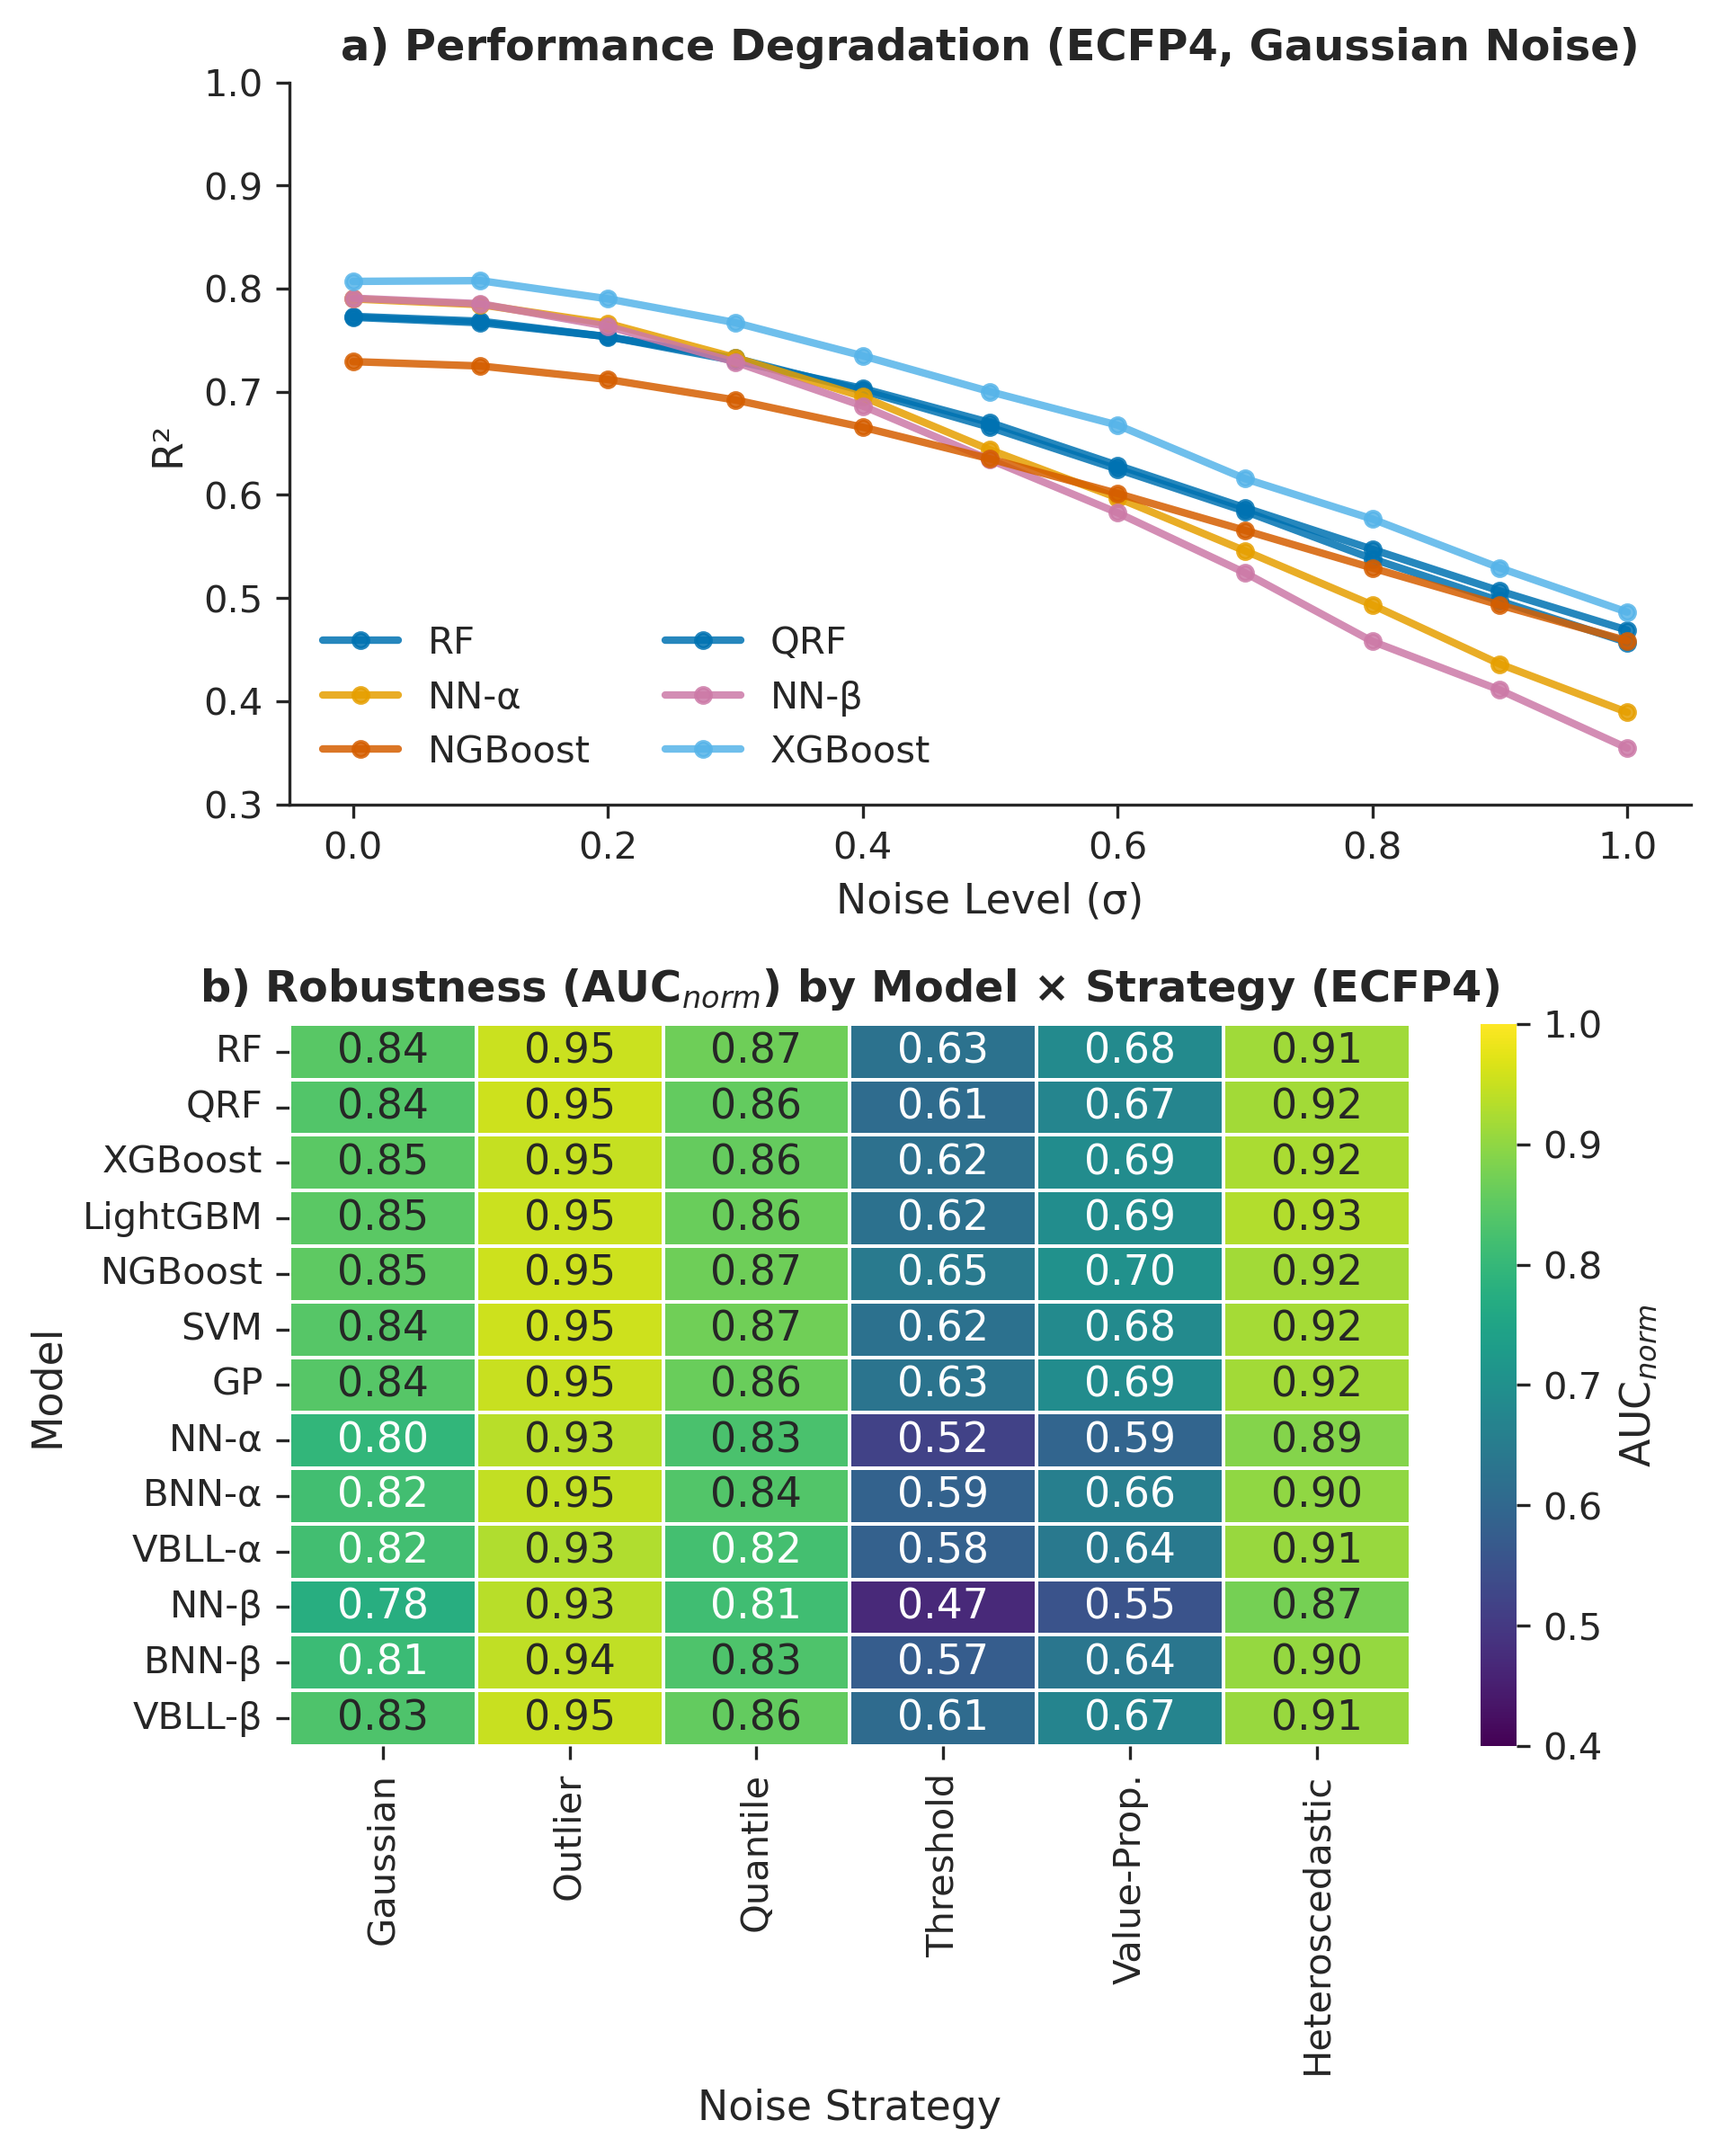
\includegraphics[width=\textwidth,height=0.78\textheight,keepaspectratio]{fig1_supp_ecfp4_overview.png}
\caption{\textbf{Global overview of noise robustness on the ECFP4 representation, evaluated on QM9 HOMO--LUMO gap.}
a) Performance degradation curves (R$^2$ versus noise level $\sigma$) under Gaussian noise. b) Noise degradation slope (NDS) heatmap across model architectures and noise strategies; lower (more negative) NDS indicates faster degradation under noise.}
\label{app:noise:ecfp4_overview}
\end{figure}


\section{Clean $R^2$ against robustness, PDV, Gaussian noise}\label{app:noise:sec:clean_r2_vs_robustness}
% Thesis appendix item: clean_r2_vs_robustness
% Seeded on 2026-09-27 from qsar_qm_models/supplementary/items/clean_r2_vs_robustness.tex by thesis_appendix/seed_from_paper.py.
% From here on this copy is edited independently of the paper. Rules: thesis_appendix/README.md.
% The lines below, down to the first blank line, are the PAPER copy's header, kept for
% provenance. They describe the paper file, not this one: in particular a GENERATED
% notice there does not apply here, and this copy may be edited by hand.
% Supplementary item: clean_r2_vs_robustness
% Split out of additional_files.tex on 2026-09-27, where it was Additional file 7 (Baseline R^2 vs NDS scatter (was Supp Figure S2)).
% Content unchanged apart from: the heading line removed (the build writes it), the old
% 'Table S*/Figure S*' caption prefix replaced by \SuppFile{}, and the label renamed to supp:clean_r2_vs_robustness.
% Rules: supplementary/README.md.

\begin{figure}[H]
\centering
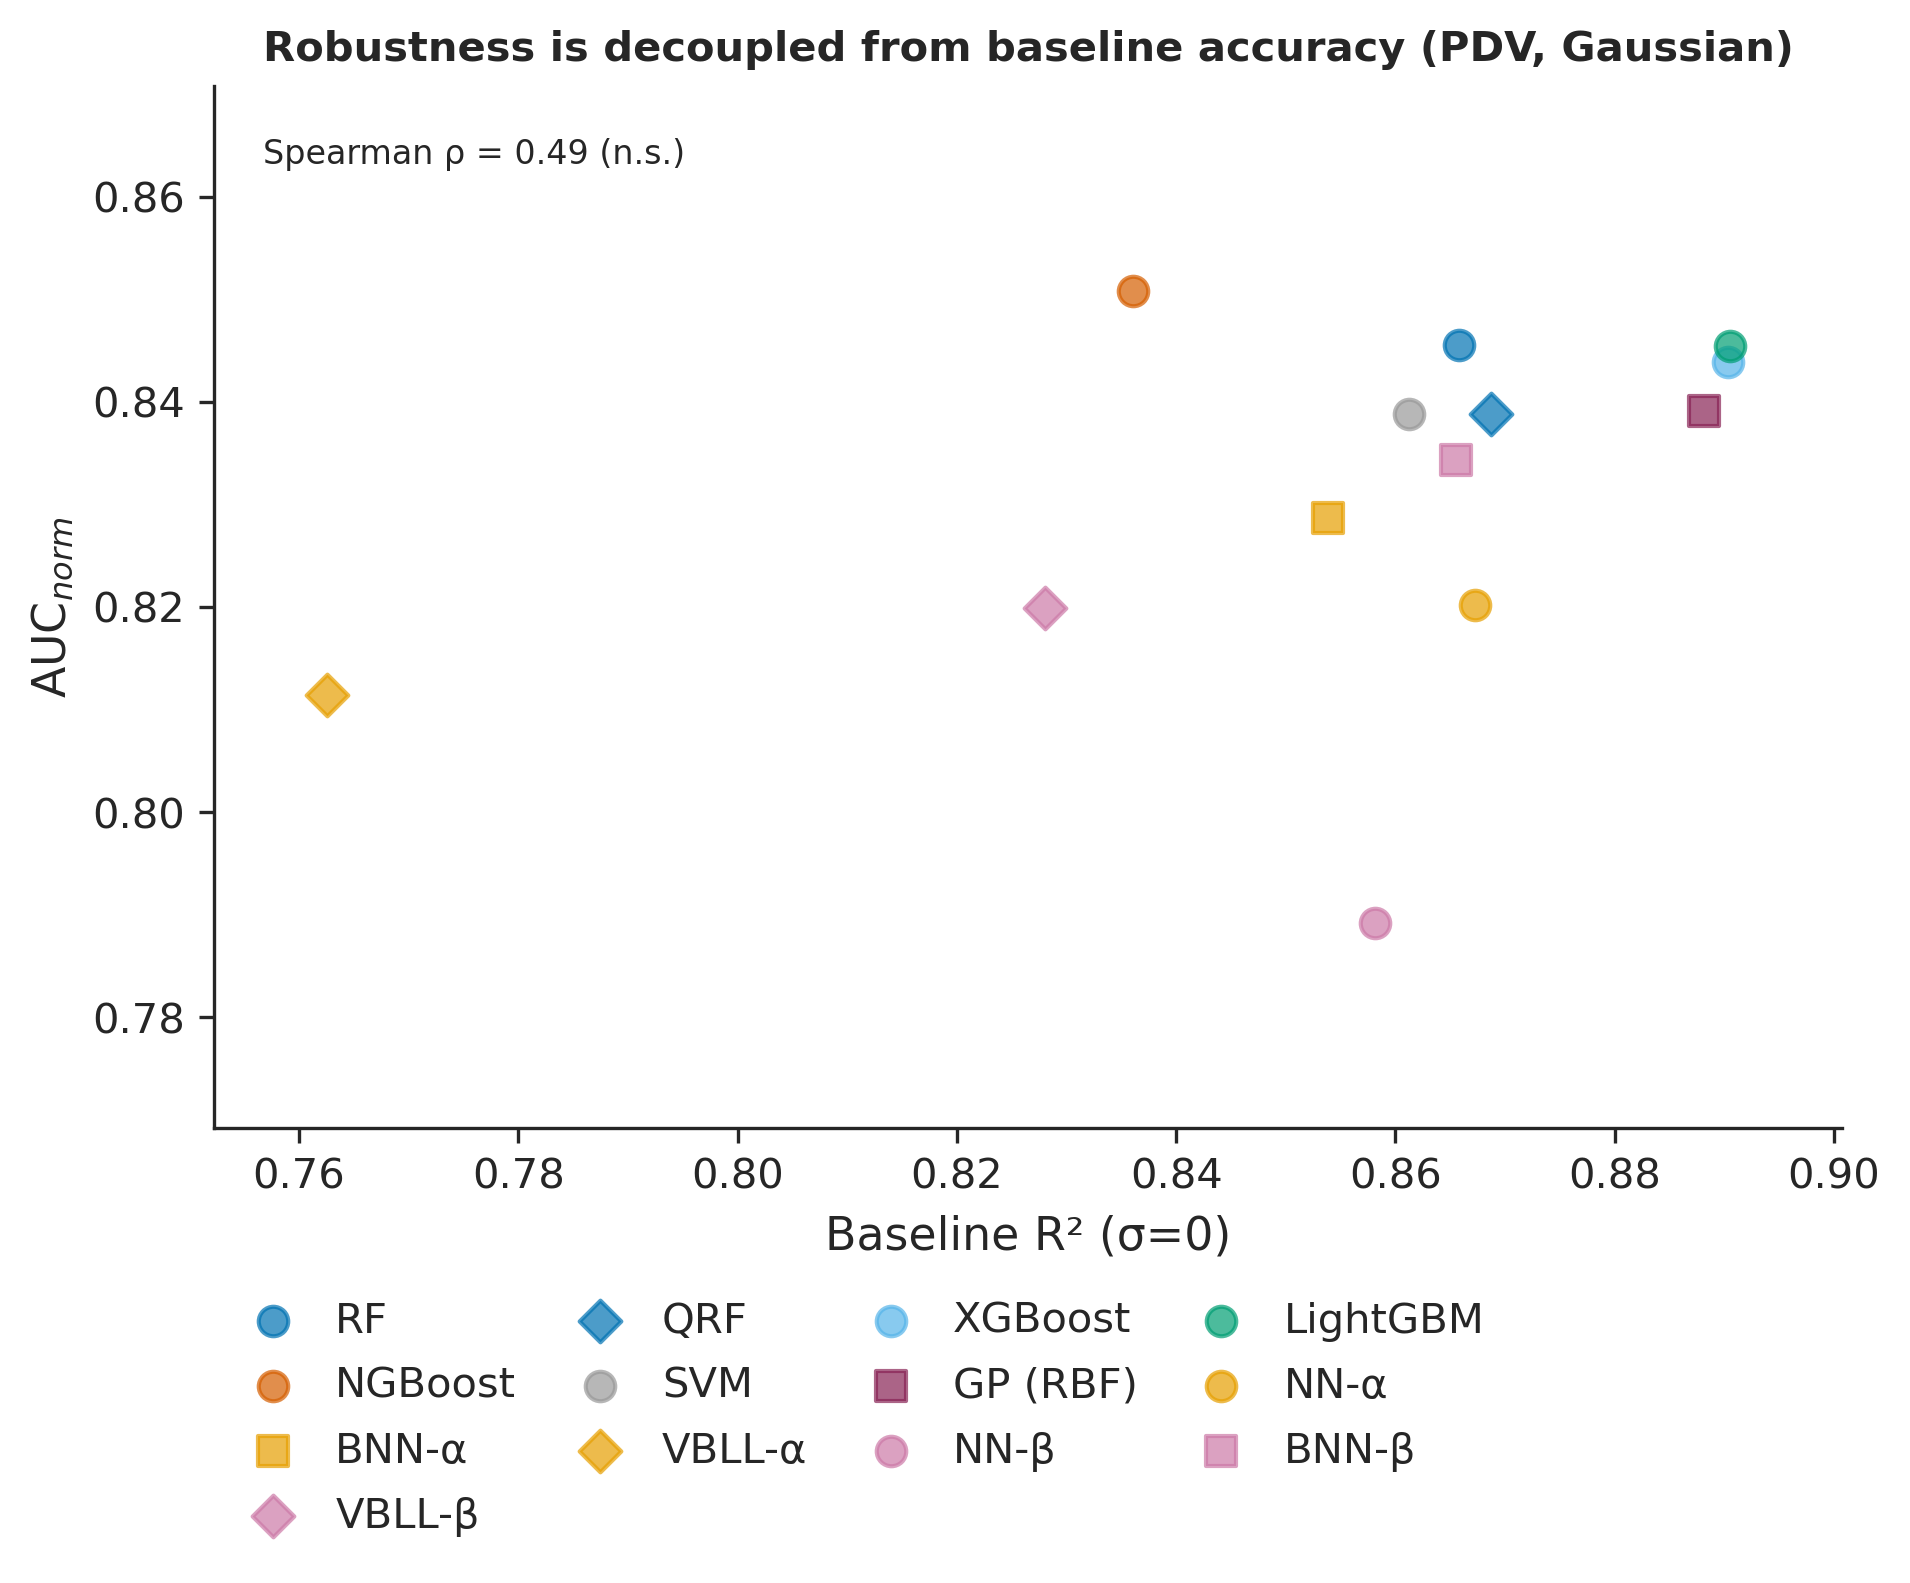
\includegraphics[width=\textwidth]{fig3_ranking_consistency.png}
\caption{\textbf{Baseline R$^2$ versus noise degradation slope (NDS) scatter for all models on the physicochemical descriptor vector (PDV) representation under Gaussian noise, on the QM9 HOMO--LUMO gap.}
Lower (more negative) NDS indicates faster performance loss under noise.}
\label{app:noise:clean_r2_vs_robustness}
\end{figure}


\section{Bayesian transformation effects by representation}\label{app:noise:sec:bayesian_transformation_tests}
% Thesis appendix item: bayesian_transformation_tests
% Seeded on 2026-09-27 from qsar_qm_models/supplementary/items/bayesian_transformation_tests.tex by thesis_appendix/seed_from_paper.py.
% From here on this copy is edited independently of the paper. Rules: thesis_appendix/README.md.
% The lines below, down to the first blank line, are the PAPER copy's header, kept for
% provenance. They describe the paper file, not this one: in particular a GENERATED
% notice there does not apply here, and this copy may be edited by hand.
% Supplementary item: bayesian_transformation_tests
% Split out of additional_files.tex on 2026-09-27, where it was Additional file 8 (NN Bayesian transformation effects (was Supp Table S6)).
% Content unchanged apart from: the heading line removed (the build writes it), the old
% 'Table S*/Figure S*' caption prefix replaced by \SuppFile{}, and the label renamed to supp:bayesian_transformation_tests.
% Rules: supplementary/README.md.

\begin{table}[H]
\centering
\caption{\textbf{Neural network Bayesian transformation effects on noise degradation slope (NDS) by representation, on the QM9 HOMO--LUMO gap.}
Positive $\Delta$ NDS indicates the Bayesian variant is more robust (less negative slope) than its deterministic counterpart.}
\label{app:noise:bayesian_transformation_tests}
\small
\begin{tabular}{llrrrr}
\toprule
\textbf{Model} & \textbf{Representation} & \textbf{Baseline R$^2$} & \textbf{NN-$\beta$ NDS} & \textbf{BNN-$\beta$ NDS} & \textbf{$\Delta$ NDS} \\
\midrule
NN-$\beta$ & ECFP4 & 0.791 & $-0.464$ & $-0.388$ & $+0.076$ \\
NN-$\beta$ & PDV & 0.858 & $-0.487$ & $-0.382$ & $+0.106$ \\
NN-$\beta$ & SMILES & 0.721 & $-0.558$ & $-0.365$ & $+0.193$ \\
\bottomrule
\end{tabular}
\end{table}


\section{Uncertainty metrics for probabilistic models on ECFP4}\label{app:noise:sec:uncertainty_metrics_ecfp4}
% Thesis appendix item: uncertainty_metrics_ecfp4
% Seeded on 2026-09-27 from qsar_qm_models/supplementary/items/uncertainty_metrics_ecfp4.tex by thesis_appendix/seed_from_paper.py.
% From here on this copy is edited independently of the paper. Rules: thesis_appendix/README.md.
% The lines below, down to the first blank line, are the PAPER copy's header, kept for
% provenance. They describe the paper file, not this one: in particular a GENERATED
% notice there does not apply here, and this copy may be edited by hand.
% Supplementary item: uncertainty_metrics_ecfp4
% Split out of additional_files.tex on 2026-09-27, where it was Additional file 9 (Uncertainty metrics ECFP4 (was Supp Table S8)).
% Content unchanged apart from: the heading line removed (the build writes it), the old
% 'Table S*/Figure S*' caption prefix replaced by \SuppFile{}, and the label renamed to supp:uncertainty_metrics_ecfp4.
% Rules: supplementary/README.md.

\begin{table}[H]
\centering
\caption{\textbf{Uncertainty quantification metrics for probabilistic models on the ECFP4 representation (Gaussian noise strategy) on the QM9 HOMO--LUMO gap.}
Unc-Error $\rho$: Spearman correlation between predicted uncertainty and absolute prediction error. Unc-Noise $\rho$: Spearman correlation between predicted uncertainty and injected noise level $\sigma$. ECE: expected calibration error (lower = better-calibrated). Coverage targets: 68\% ($1\sigma$), 95\% ($2\sigma$).}
\label{app:noise:uncertainty_metrics_ecfp4}
\small
\begin{tabular}{lrrrrr}
\toprule
\textbf{Model} & \textbf{Unc-Error $\rho$} & \textbf{Unc-Noise $\rho$} & \textbf{ECE} & \textbf{Cov.\ $1\sigma$} & \textbf{Cov.\ $2\sigma$} \\
\midrule
\textbf{QRF}     & \textbf{0.25} & 0.27 & 0.19 & 74.7\% & 94.6\% \\
\textbf{NGBoost} & 0.22 & \textbf{0.37} & \textbf{0.11} & 69.2\% & 94.2\% \\
GP               & 0.18 & 0.34 & 0.23 & 78.6\% & 96.0\% \\
BNN-$\beta$      & 0.20 & 0.37 & 0.29 & 78.6\% & 95.2\% \\
BNN-$\alpha$     & 0.15 & 0.32 & 0.24 & 76.6\% & 95.1\% \\
VBLL-$\beta$     & 0.19 & 0.34 & 0.19 & 73.9\% & 95.5\% \\
VBLL-$\alpha$    & 0.11 & 0.31 & 0.22 & 74.5\% & 95.1\% \\
\bottomrule
\end{tabular}
\end{table}


\section{Variance decomposition on the three assay datasets}\label{app:noise:sec:assay_variance_decomposition}
% Thesis appendix item: assay_variance_decomposition
% Seeded on 2026-09-27 from qsar_qm_models/supplementary/items/assay_variance_decomposition.tex by thesis_appendix/seed_from_paper.py.
% From here on this copy is edited independently of the paper. Rules: thesis_appendix/README.md.
% The lines below, down to the first blank line, are the PAPER copy's header, kept for
% provenance. They describe the paper file, not this one: in particular a GENERATED
% notice there does not apply here, and this copy may be edited by hand.
% Supplementary item: assay_variance_decomposition
% Split out of additional_files.tex on 2026-09-27, where it was Additional file 10 (Validation ANOVA (was Supp Figure S3)).
% Content unchanged apart from: the heading line removed (the build writes it), the old
% 'Table S*/Figure S*' caption prefix replaced by \SuppFile{}, and the label renamed to supp:assay_variance_decomposition.
% Rules: supplementary/README.md.

\begin{figure}[H]
\centering
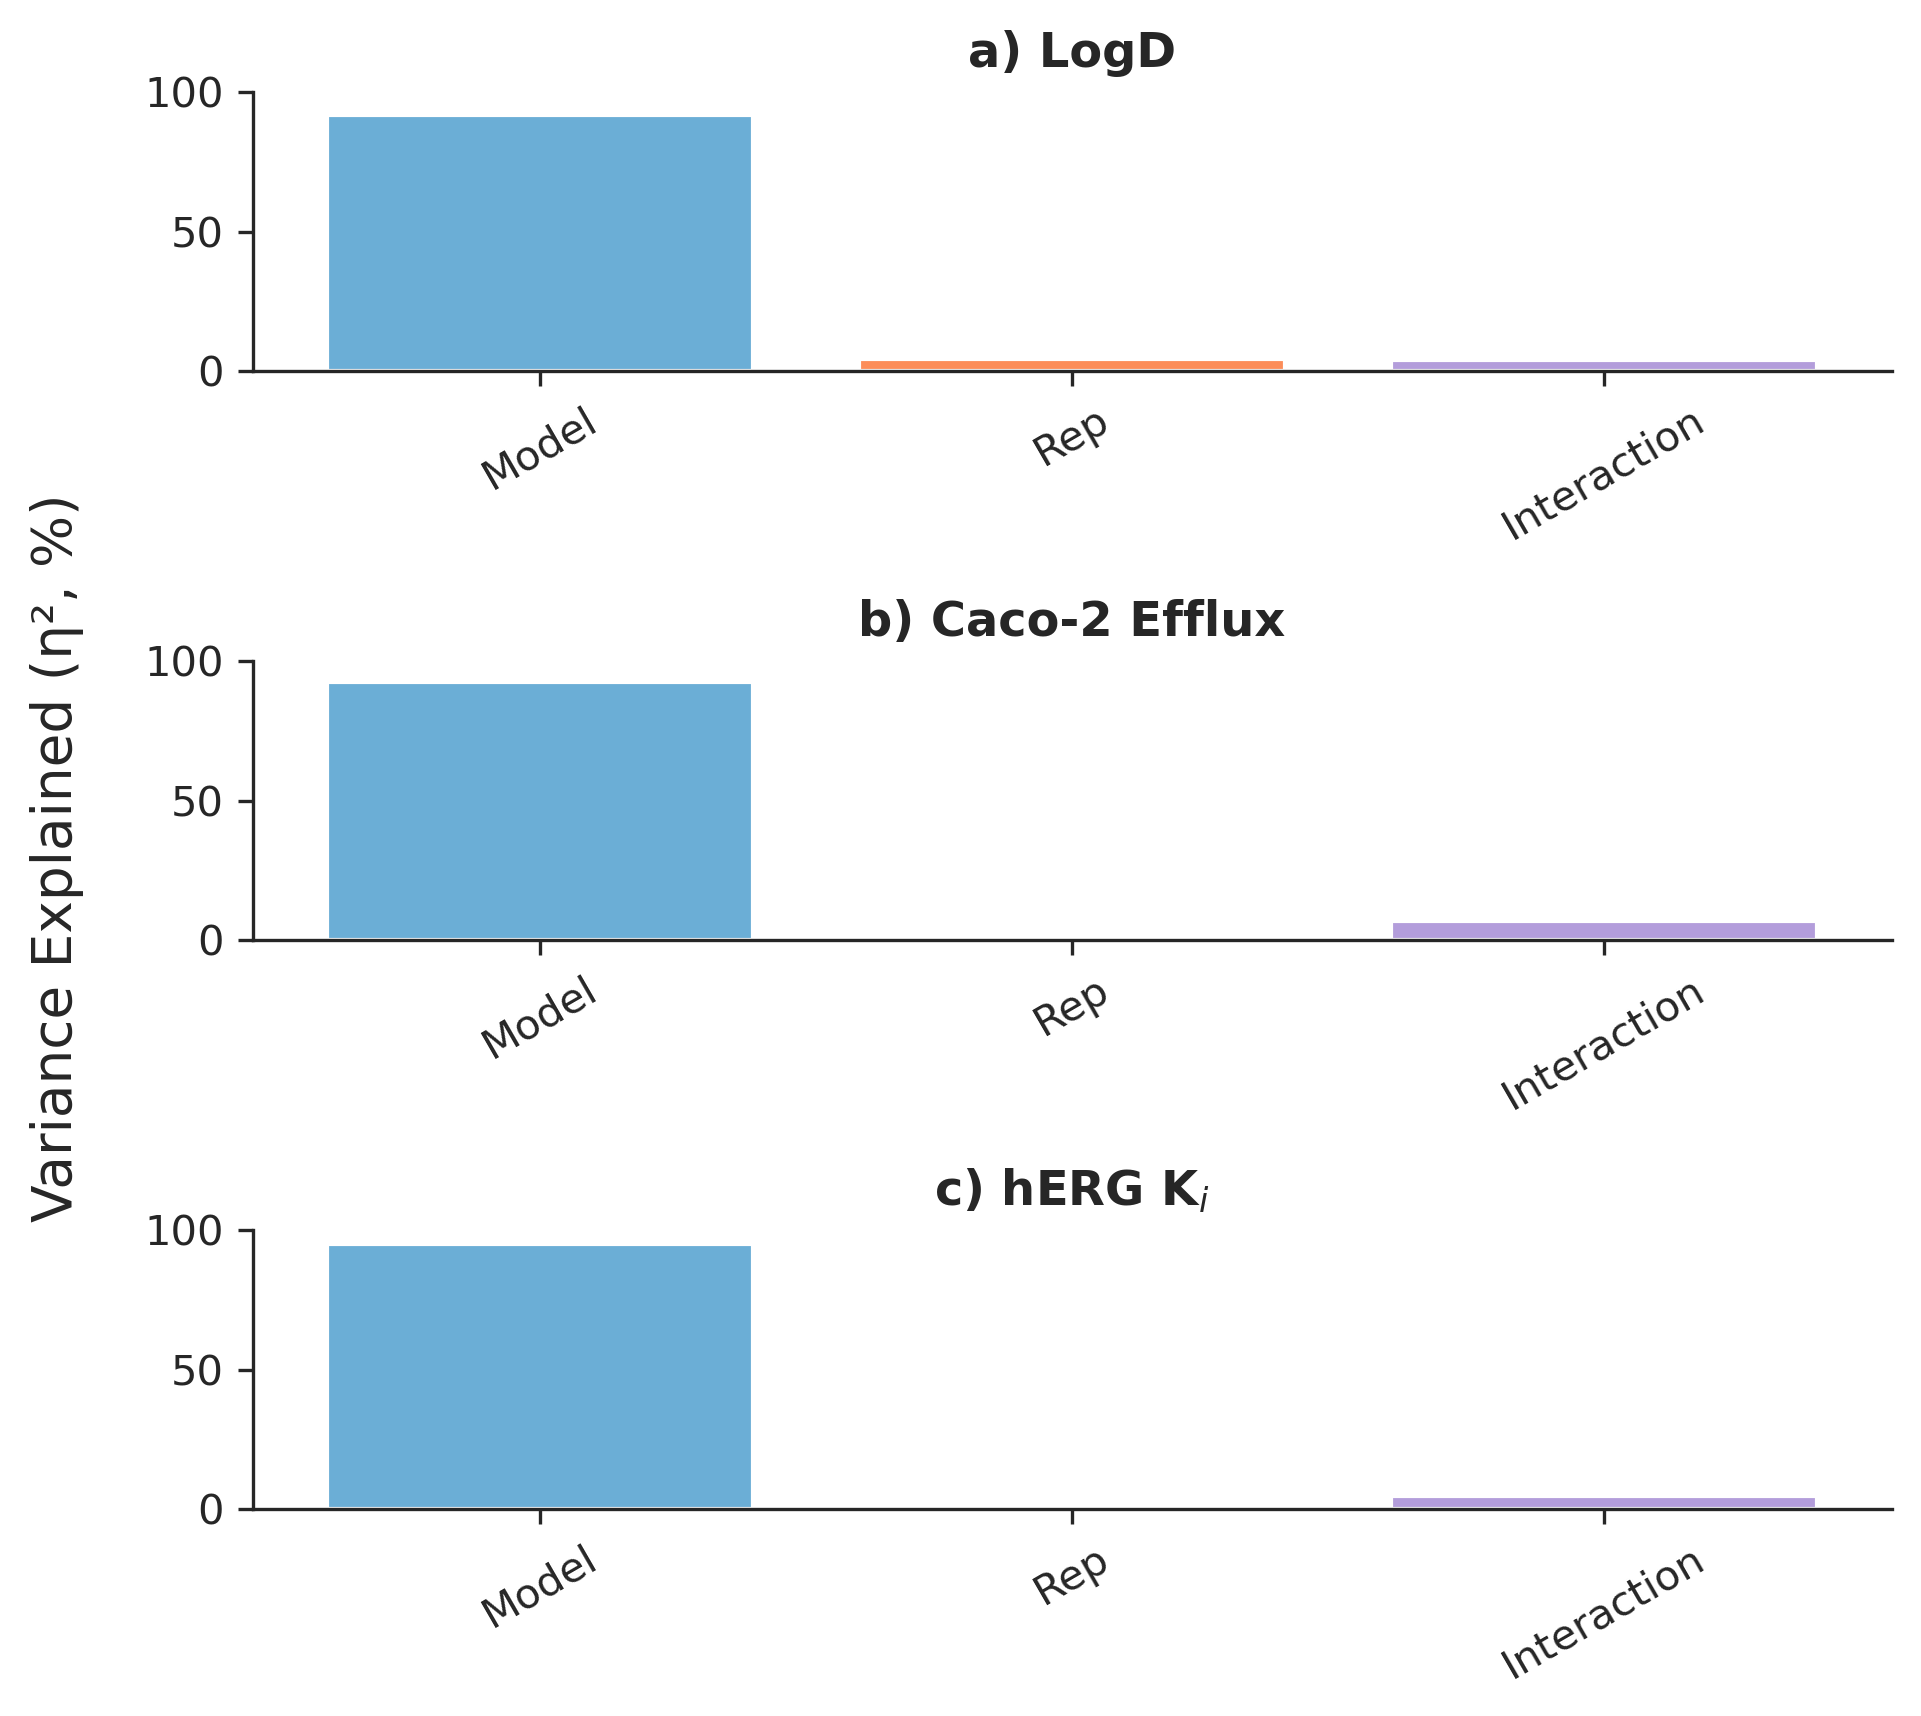
\includegraphics[width=\textwidth]{fig_validation_anova.png}
\caption{\textbf{ANOVA variance decomposition ($\eta^2$, \%) on external validation datasets: a) LogD, b) Caco-2 Efflux, and c) hERG K$_i$.}
Model, representation, and interaction contributions to noise degradation slope (NDS) variance for each dataset; lower (more negative) NDS indicates faster performance loss under noise.}
\label{app:noise:assay_variance_decomposition}
\end{figure}


\section{RF against QRF on the three assay datasets}\label{app:noise:sec:rf_vs_qrf_assay}
% Thesis appendix item: rf_vs_qrf_assay
% Seeded on 2026-09-27 from qsar_qm_models/supplementary/items/rf_vs_qrf_assay.tex by thesis_appendix/seed_from_paper.py.
% From here on this copy is edited independently of the paper. Rules: thesis_appendix/README.md.
% The lines below, down to the first blank line, are the PAPER copy's header, kept for
% provenance. They describe the paper file, not this one: in particular a GENERATED
% notice there does not apply here, and this copy may be edited by hand.
% Supplementary item: rf_vs_qrf_assay
% Split out of additional_files.tex on 2026-09-27, where it was Additional file 11 (RF vs QRF on validation datasets (was Supp Table S7)).
% Content unchanged apart from: the heading line removed (the build writes it), the old
% 'Table S*/Figure S*' caption prefix replaced by \SuppFile{}, and the label renamed to supp:rf_vs_qrf_assay.
% Rules: supplementary/README.md.

\begin{table}[H]
\centering
\caption{\textbf{Random forest (RF) vs quantile regression forest (QRF) noise degradation slope (NDS) on the three external validation datasets (LogD, Caco-2 Efflux, hERG K$_i$).}
Lower (more negative) NDS indicates faster degradation under noise.}
\label{app:noise:rf_vs_qrf_assay}
\small
\begin{tabular}{lrrr}
\toprule
\textbf{Dataset} & \textbf{RF NDS} & \textbf{QRF NDS} & \textbf{$\Delta$ NDS} \\
\midrule
ChEMBL-hERG-Ki     & $-0.231$ & $-0.359$ & $-0.128$ \\
OpenADMET-Caco2    & $-0.534$ & $-0.627$ & $-0.094$ \\
OpenADMET-LogD     & $-0.101$ & $-0.185$ & $-0.083$ \\
\bottomrule
\end{tabular}
\end{table}


\chapter{The search space and its defaults}\label{app:searchspace}
% ---- from THESIS_OUTLINE.md :: APPENDIX C (quoted; long bullets condensed) ----
%   C: the method's full search space and the design-experiment tables behind its defaults (Chapter 4).
%      The full vocabulary: downstream models (rf, xgboost, ridge, knn, lightgbm,
%      mlp, svm, gp, with optional catboost, dnn, cnn, bnn, ngboost); feature budgets (roughly 10
%      to 2,000, per-model capped); allocation methods (greedy, performance-weighted with its
%      weighting schemes, dominant-greedy, fixed, two-stage, stability-selection); importance
%      methods (treeshap, xgboost_gain, lightgbm_gain, permutation, kernelshap, deeplift,
%      integrated_gradients, gradientshap); internal evaluators (match, or rf/svm/lightgbm/mlp);
%      augmentation strategies; and the exact blueprint fields.
% ---- end outline extract ----
\todo[inline, color=orange!40]{Appendix C is unwritten.}
\chapter{Extended result tables}\label{app:results}
% ---- from THESIS_OUTLINE.md :: APPENDIX D (quoted; long bullets condensed) ----
%   D: extended result tables for the second-half chapters (Chapters 5 to 6), organised by the
%      featured experiments: the cross-domain summary; the information-theoretic decomposition;
%      the explainability and attribution tables; the forward-compatibility tables; the federated
%      comparator tables; the similarity-activity correlation tables; the BindingDB
%      ground-truth-noise table; and the remediation and noise-estimation tables.
% ---- end outline extract ----
\todo[inline, color=orange!40]{Appendix D is unwritten.}
\chapter{Data and code availability}\label{app:availability}
% ---- from THESIS_OUTLINE.md :: APPENDIX E (quoted; long bullets condensed) ----
%   E: data and code availability (all chapters). The full statement covers three distinct
%      software artifacts. (1) NoiseInject: the open-source benchmarking framework, MIT, at
%      github.com/adpunt/noise_inject, archived on Zenodo; released. (2) The standalone Rust and
%      Python chemical-processing and precompute pipeline. (3) The KIRBy research codebase: pure
%      Python. KIRBy contains no Rust; it operates on precomputed numpy feature matrices.
% ---- end outline extract ----

% [NI 629-640] her NoiseInject availability statement + the Springer-style itemised
% block the outline asks for. Two more such blocks are needed (precompute pipeline, KIRBy).
The NoiseInject benchmarking framework, implementing all six regression and six classification noise injection strategies together with the robustness metrics (noise degradation slope and retention) and uncertainty-calibration metrics (ECE, coverage at $1\sigma$/$2\sigma$, mean interval width, and uncertainty--error / uncertainty--noise correlation) described in this work, is available as an open-source Python package under an MIT license \citep{noiseinject}. It also contains optional reference wrappers (a Gaussian process, split-conformal prediction, and Monte Carlo dropout) that produce per-sample uncertainty for use with these metrics. NoiseInject is model-agnostic, operates on label arrays (NumPy arrays or pandas Series), and is designed to integrate into existing cheminformatics or other data pipelines. Worked examples covering molecular-descriptor, fingerprint, and GNN-embedding workflows are provided in the repository.

\begin{itemize}
    \item Project name: NoiseInject
    \item Project home page: \url{https://github.com/adpunt/noise_inject}
    \item Archived version: \url{https://doi.org/10.5281/zenodo.20532710}
    \item Operating system(s): Platform independent
    \item Programming language: Python
    \item Other requirements: See repository \texttt{requirements.txt} for the full dependency list
    \item License: MIT
    \item Any restrictions to use by non-academics: None
\end{itemize}

% [NI 654] authors' contributions, for the front-matter declaration.
A.P. implemented the NoiseInject framework, conducted all experiments, and drafted the manuscript. T.H., S.W., and G.M. supervised the project, contributed to the experimental design, and revised the manuscript. All authors read and approved the final manuscript.
\todo[inline, color=orange!40]{Appendix E: add itemised blocks for the Rust/Python precompute pipeline and for KIRBy, plus the Lhasa/Effiris redistribution caveat.}

%%
%%----------------------------------------------------------------------------
%% !! THREE THINGS TO DO BEFORE THIS COMPILES !!
%%
%% 1. PREAMBLE: use KIRBy/main.tex (report class, amssymb, per-chapter counters, front matter).
%%    The old Confirmation_Report/main.tex will NOT compile this file.
%%
%% 2. BIBLIOGRAPHY.
%%    COMPILE-VERIFIED (pdflatex + bibtex, plainnat): 51 cited keys render as [?].
%%
%%    (a) 2 exist in refs.bib but under a DIFFERENT CASE. BibTeX resolves the lookup
%%        case-insensitively, but natbib matches the emitted \bibitem label case-SENSITIVELY,
%%        so these silently print [?]. Fix by matching the case:
%%           \citep{Lakshminarayanan2017}  ->  refs.bib entry is  lakshminarayanan2017
%%           \citep{Ross2022}  ->  refs.bib entry is  ross2022
%%
%%    (b) 49 have no entry in refs.bib at all:
%%           Ambroise2002            Bellman1961             Boiko2025               Bommasani2021
%%           Cawley2010              Cichonska2018           Demsar2006              Dong2020
%%           Elnaggar2022            ElNahhas2025            FernandezDelgado2014    Gonen2011
%%           Hughes1968              jaeger2018mol2vec       Jiang2021               jorner2021
%%           ke2017lightgbm          Kenlay2024              Kumar2022               landrum2024
%%           Lin2023                 Mayr2018                NadeauBengio2003        Ng2004
%%           Nogueira2018            noiseinject             Notin2023               Olsen2022
%%           openadmet               qm9_dataset             Ruffolo2021             Schmirler2024
%%           Song2026                Stahlschmidt2022        Steyaert2023            Thornton2013
%%           Tibshirani2015          Tishby2015              Vabalas2019             Valsecchi2020
%%           Vapnik1995              Vieira2026              Wallach2018             Walters2023
%%           Wang2021                Yang2019                Zdrazil2023             Zeng2022
%%           Zhang2024
%%
%%    Nearly all of (b) arrive with the KIRBy chapters from PAPER_DRAFT.md; their entries
%%    live in KIRBy/PAPER_REFERENCES.md. The rest arrive with the updated NoiseInject text
%%    and its availability statement: jorner2021, ke2017lightgbm, landrum2024, noiseinject,
%%    openadmet, qm9_dataset, lhasa, Vapnik1995, Walters2023, Zdrazil2023, and
%%    jaeger2018mol2vec (= refs.bib's existing Jaeger2018).
%%
%% 3. refs.bib: FIXED in KIRBy/refs.bib (use that copy, not the one in Confirmation_Report).
%%    Two unescaped ampersands were FATAL LaTeX errors, both pre-existing:
%%       refs.bib:1755   title={Sort &amp; Slice: ...}          ->  Sort \& Slice
%%       refs.bib:1859   booktitle={... Knowledge Discovery & Data Mining (KDD)} -> \&
%%    With those two fixed the thesis builds clean: 69 pages, 0 errors, 0 undefined refs.
%%    (refs.bib also has 5 duplicate entries: bibtex 'Repeated entry' at 749, 1330, 1645,
%%     1947, 1965. Harmless but worth pruning.)
%%
%% 4. CHAPTERS vs SECTIONS. The confirmation report used \section for what its
%%    prose calls "Chapter N", under \documentclass{article}. That convention is
%%    preserved here so the cloned Overleaf project still compiles untouched.
%%    To get real chapters: switch main.tex to \documentclass{report} and run
%%       sed -i '' 's/^\\section{/\\chapter{/; s/^\\subsubsection{/\\paragraph{/; s/^\\subsection{/\\section{/' thesis.tex
%%    (do the substitutions in that order).
%%
%%----------------------------------------------------------------------------
%% REMOVED relative to the confirmation report:
%%   * old ch.4 "Exploring techniques for learning with noisy labels for QSAR"
%%     -- preliminary; condensed to its motivating findings in Sec 4.1 below,
%%     and measured properly in ch.6 per the outline.
%%   * old ch.3's entire results section, and its methods -- superseded wholesale
%%     by noise_inject.tex.
%%   * the NSI (noise sensitivity index) metric -- noise_inject.tex replaces it
%%     with NDS (noise degradation slope). Retention is kept.
%%   * the confirmation-report Timeline subsection.
%%
%% CROSS-REFERENCES TO FIX: chapter numbers inside carried-over prose still refer
%% to the confirmation report's numbering. Every one is flagged inline with
%%   % TODO(xref)
%% Old ch.3 -> new ch.3 (robustness and uncertainty, merged 2026-09-27);  old ch.4 (LNL) -> new Sec 4.1;
%% old ch.5 -> ch.4-6.
%%============================================================================

%%========================= FRONT MATTER =====================================
% Front matter lives in main.tex. The outline asks for the following, none of
% which exists yet in the confirmation report. Listed here so nothing is lost.

% ---- from THESIS_OUTLINE.md :: FRONT MATTER (quoted; long bullets condensed) ----
%   Title page.
%   Acknowledgements (Garrett Morris; the Lhasa supervisors Thierry Hanser and Stephane
%     Werner; the EPSRC Centre for Doctoral Training, grant EP/S024093/1; OPIG; group; family).
%   Abstract (about one page; the noise problem in molecular property prediction, then one
%     clause per chapter in order, then the open-source NoiseInject note).
%   Contents.  List of Figures.  List of Tables.
%   Abbreviations (QSAR, ECFP4, SNS, PDV, OHE, MHG-GNN, GNN, MLP, RF, QRF, XGBoost, NGBoost,
%     GP, SVM, BNN, VBLL, LNL, NDS, ECE, ANOVA, RMSE, ROC-AUC, F1, PCA, mRMR, RFE, RBF, DFT,
%     ADME, and the rest, spelled out once here so the chapters can use them bare).
%   Declaration (the thesis includes the jointly authored NoiseInject paper and the Lhasa
%     and OPIG collaborations; a short statement of the author's own contribution). A signed
%     Statement of Authorship for the jointly authored NoiseInject paper is included, as the
%     Oxford requirement for joint work, covering Chapter 3.
%   Data and Code Availability (three distinct software artifacts: (1) NoiseInject, MIT,
%     github.com/adpunt/noise_inject; (2) a standalone Rust and Python chemical-processing and
%     precompute pipeline, to be simplified and released separately; (3) the KIRBy research
%     codebase (pure Python). KIRBy contains no Rust.
%   List of Publications: the NoiseInject paper (Punt, Hanser, Werner and Morris, in
%     preparation for the Journal of Cheminformatics); the two planned hybrid-representation
%     papers (Chapters 5 and 6); the UK-QSAR conference presentation; the OPIG Blopig posts;
%     and the open-source software.
% ---- end outline extract ----
% TODO: The confirmation report's Abbreviations list (main.tex) is stale: it still lists
% TODO: NSI and OHE-era entries and omits NDS, VBLL, ANOVA, ICC, LightGBM, SVM, MHG-GNN.
% TODO: noise_inject.tex lines 588-623 hold an updated list -- merge it into main.tex.

\chapter{Introduction}\label{chap:intro}

New avenues in the drug discovery pipeline have opened up thanks to advances in large dataset collection, analysis, and computation. Therapeutic targets are identified, potential drug candidates are screened and optimized, and the most promising of these go on to pre-clinical and clinical trials \citep{Lill2007}. There are various methods by which potential drug candidates can be screened. Virtual screening allows for the rapid and large-scale analysis of libraries of compounds, and is a particularly useful approach used to speed up the drug discovery process \citep{Neves2018}. One standard screening method is the prediction of bioactivities and pharmacological properties of such candidates. There is a long history of using Quantitative Structure-Activity Relationship (QSAR) models to make these predictions, to act as a filter for compounds with undesirable properties, and thus reduce the time and cost associated with experimental screening \citep{Sabando2021}. QSAR models aim to predict the relationship between a molecule's molecular features as encoded within a particular molecular representation and a desired molecular property \citep{Sabando2021} of interest. A QSAR model typically consists of a molecular representation paired with a machine learning (ML) model. An ideal molecular representation will allow a model to learn only the relevant information about each molecule with respect to the target property. Representations are either `static' hand-crafted descriptors or circular fingerprints that encode predefined structural and physicochemical features \citep{Rogers2010, David2020, sns, avalon}; or learned representations, where the encoding is derived from a predictive model, often taken from the activations of the final layer of a neural network, or a latent space embedding \citep{Sabando2021, kishimoto2023}. 

QSAR models are of course, sensitive to the quality of the input data on which they are trained. Experimental noise can arise from measurement errors, variability under experimental conditions, varying provenance of the data, and intrinsic biological and chemical variability. Even the very measures of model performance may be flawed if test and validation sets are laden with noise. \citet{Kolmar2021} show that the variance associated with experimental data can contribute more to prediction error than the model’s own error. There is also a limit to how much noise the model can tolerate; \citet{jorner2021} found that once the model error approaches the magnitude of the experimental measurement error on labels, adding more training data yields diminishing returns in predictive performance. In the context of activity prediction, the inherent variability within experimental setups and assays, batch effects, measurement errors, and biological variability introduce additional layers of complexity \citep{Kolmar2021, Fourches2010}. All of this increases the likelihood of encountering noise in the data \citep{Fang2022}. Even the molecular representations in the training data themselves may be incorrect or misleading \citep{Walters2023}, and chemical datasets contain too few repeat measurements of each compound to characterise the distribution the label is drawn from. Thus, models treat a single label as the population mean \citep{Kolmar2021}. Repeat measurements of the same compound-target pair disagree by about $0.68$ log units for pIC$_{50}$, and by about $0.54$ log units for pK$_i$ \citep{Kalliokoski2013, Kramer2012}. Measurements from a single assay lowers the mean disagreement from $0.50$ to $0.27$ log units \citep{landrum2024}.  

% TODO: do I need citations here? for the similarity stuff
% TODO: rephrase: However, all of the methods that used simiarity metrics failed, even when I tried using different molecular representations and vector operations 
This thesis addresses the challenge of conducting molecular property prediction when the underlying experimental data contain noisy labels. My initial research question is which combinations of molecular representations and predictive model architectures maintain predictive performance under label corruption, and whether probabilistic methods that estimate uncertainty justify their additional complexity. As I will show, both model and representation choice dominate predictive performance on clean data, however, this relationship inverts under label corruption as predictive architecture becomes the primary factor in determining noise robustness.  Most existing work on noise in QSAR modelings assumes that label noise can be modeled as random error drawn from a Gaussian distribution, and they evaluate either molecular representations or predictive model architectures in isolation. \cite{Cortes2015} examined 12 algorithms across multiple noise levels but used fixed representations. Studies that compare representations are typically done on clean data. No work has systematically compared the relative importance of representation versus architecture choice for noise robustness, assessed whether probabilistic methods justify their computational overhead in noisy settings, or tested whether findings generalize across different corruption patterns and molecular property types.

Building on these findings, I began exploring techniques involving learning with noisy labels and noise mitigation. Many of these methods incorporate measures of molecular similarity, relying on the assumption that molecules which are similar in structure share similar properties. However, all of the methods that used simiarity estimates failed, even when I tried varying the molecular representations and vector operations from the standard ECFP4 and Tanimoto coefficient. I hypothesized that to generate accurate similarity estimates, you need a specialised molecular representation who's features relate directly to similarity in that molecular domain. This brings me to my next research question, how do you select the best set of features for a given prediction task? I will outline how I developed an adaptive feature selection methodology that takes in a set of molecular representations, identifies each representation's most important features, and combines a select set of those top features into a new hybrid representation. I will then demonstrate how it improve performance across a range of predictive tasks beyond the small molecule space, and how it can be applied to the context of similarity estimation and downstream noise mitigation methods. 
% TODO: how do I end this? Check other theses


\section{The questions this thesis asks}

% ---- from THESIS_OUTLINE.md :: 1.3  The questions this thesis asks (quoted; long bullets condensed) ----
%   Under label noise, which matters more for robustness, the representation or the model
%     architecture, and can probabilistic models recover usable uncertainty estimates that
%     track that noise?
%   Building on those answers: can the representation itself be adapted to make prediction
%     more robust, and to make molecular similarity and noise estimation more reliable?
% ---- end outline extract ----

% [NI 202] the three questions, as stated in the NoiseInject paper.
This research addresses three main aspects of the robustness of QSAR models under label noise. First, we investigate the contributions of molecular representation and model architecture on both overall predictive performance and, more specifically, noise robustness. Second, we compare how noise-robust probabilistic models perform versus their deterministic counterparts, and whether their uncertainty estimates correlate with prediction error or label noise under noisy conditions. Third, we assess the generalizability of noise-robustness patterns across different noise-injection mechanisms and molecular properties. Together, these questions aim to identify what, if anything, makes a QSAR model robust to noise. Finally, we introduce NoiseInject, an open-source Python package for benchmarking noise robustness and uncertainty quantification in machine learning models.

\section{From noise robustness to adaptive representations}

% ---- from THESIS_OUTLINE.md :: 1.4  From noise robustness to adaptive representations (quoted; long bullets condensed) ----
%   The first half establishes that, under noise, the model dominates robustness while the
%     representation governs clean performance, and that only certain probabilistic models
%     sense per-sample noise.
%   An exploratory study of learning-with-noisy-labels methods then showed that the
%     approaches relying on molecular similarity fail under noise, which motivated the second
%     half: an adaptive hybrid representation that builds a compact, informative representation
%     from several others, and in doing so repairs the notion of similarity those methods
%     depend on.
% ---- end outline extract ----
\todo[inline, color=yellow!40]{Write Sec 1.4 from the outline bullets above. The raw material is Section~\ref{sec:lnl_motivation}.}

\section{Outline of the thesis and contributions}

% TODO: The confirmation report's 'Report Overview' [CR 85-97] described a SIX-chapter report
% TODO: including the LNL chapter. It is deliberately NOT carried over -- it is wrong for the
% TODO: seven-chapter thesis. Rewrite from the outline bullets below, which are already
% TODO: per-chapter and in the author's own words.
% ---- from THESIS_OUTLINE.md :: 1.5  Outline of the thesis and contributions (2026-09-27 version; condensed) ----
%   Chapter 2 sets out the representations, models, noise model, and evaluation that the
%     rest of the thesis uses, and introduces NoiseInject, the open-source benchmarking framework.
%   Chapter 3 is the NoiseInject chapter (adapted from Punt, Hanser, Werner and Morris, in
%     preparation for the Journal of Cheminformatics). It decomposes the variance in performance
%     and in noise robustness across representations and model architectures; compares seven
%     noise conditions at a matched amount of noise; repeats the study on three assay datasets;
%     compares each model with its probabilistic counterpart; and asks what label noise does to
%     predicted uncertainty.
%   Chapter 4 introduces the adaptive hybrid representation, with the exploratory
%     learning-with-noisy-labels work as its motivation.
%   Chapter 5 is the first of the two planned method papers. It will test when and why the
%     hybrid representation helps, that it is explainable, and that it extends to new
%     embeddings and to federated data.
%   Chapter 6 is the second planned method paper. It will return to molecular similarity and
%     label noise, testing whether the hybrid representation gives a more property-aware
%     similarity and improves noise estimation.
%   Chapter 7 draws the argument together and then develops the main open directions.
% ---- end outline extract ----
\todo[inline, color=yellow!40]{Write Sec 1.5 from the outline bullets above.}

\section{Collaborations and funding}

% ---- from THESIS_OUTLINE.md :: 1.6  Collaborations and funding (quoted; long bullets condensed) ----
%   The EPSRC Centre for Doctoral Training (grant EP/S024093/1); Lhasa Limited (label-noise
%     framing and the federated work); OPIG (antibody and protein datasets and the Blopig
%     collaboration).
% ---- end outline extract ----
\todo[inline, color=yellow!40]{Write Sec 1.6.}

\pagebreak
% \label{sec2} resolves \ref{sec2} in the fig:global_overview caption carried from
% noise_inject.tex, where it pointed at that paper's Methods section.
\chapter{Background}\label{chap:background}\label{sec2}

\section{Introduction}

% [CR 17] the lead-in sentence that used to close the confirmation report's intro.
I will now break down the two components of QSAR models: molecular representations and predictive models:

\section{Molecular Representations in QSAR}

% TODO: Outline Sec 2.1 additionally asks for, and the text below does NOT yet cover:
% TODO:   - Definition 2.1 (molecular representation / featurization) as a numbered definition
% TODO:   - a comparison table (Table 2.1) closing the section
% TODO:   - MACCS keys (Durant et al. 2002) and Avalon as named fingerprints
% TODO:   - mordred descriptors (Moriwaki et al. 2018); MolFormer (Ross et al. 2022)
% TODO:   - protein/antibody language-model embeddings (ESM-2, ESM-C, ESM3, SaProt, AbLang2,
% TODO:     AntiBERTy, IgT5), introduced here so ch.5 can refer back  <- WHOLE MISSING SUBSECTION
% [CR 21-54] carried whole, incl. Figure `molecular_representations.png` (= outline Fig 2.1).
The success of machine learning hinges on the quality of input data. Although the quality can refer to noise, which the majority of my work is centered around, in this case I'm talking about the type of input labels. Molecular representations provide different features with which QSAR models and noise detection techniques can be learned. However, a potential bottleneck on larger data sets should be noted; the more complex the data structure, the greater the computational cost. For smaller data sets, the number of parameters is limited by the size of the training set, to prevent overfitting. 

\begin{figure}[h]
	\centering 
	\includegraphics[width=1.05\textwidth]{molecular_representations.png}	
    \caption{\label{fig:molecular_representations}Visualisation of the molecule \lstinline{O=C1C=CN(C1)C=O} using three different methods: a) ECFP4 showing the molecule broken into substructures with circular neighbourhoods for each atom. Each substructure is hashed to produce unique identifiers, which are then compiled into a binary bit vector representing the presence or absence of specific substructures. b) SMILES tokenization and one-hot encoding of the molecule. The SMILES string is tokenized, and using a vocabulary of the most common tokens, these tokens are converted into a one-hot encoded matrix. c) Molecular graph representation where nodes represent atoms and edges represent bonds.}
\end{figure}

One of the most common and intuitive molecular representations are Simplified Molecular-Input Line-Entry System (SMILES) strings which consist of a sequence of ASCII characters generated by a fixed set of rules to specify a given chemical identity \citep{Weininger1988}. A common way to use SMILES strings as inputs to QSAR models is to tokenize and one-hot-encode them rather than to use the strings themselves \citep{TeachOpenCADD2023}. The strings are tokenized into atomic branches and symbols and mapped to indices of a vocabulary, and finally converted into binary vectors using one-hot encodings \citep{TeachOpenCADD2023}. This representation, referred to as one-hot-encoded SMILES, allows models to process molecular structures as bit-vector-based fingerprints or as sequences of vectors. Sequence-based models such as recurrent neural networks and transformers have proven to be particularly successful in capturing text semantics within a sequence. When applied to raw or one hot encoded (OHE) SMILES strings, these models can effectively capture the structure of the molecule in its textual representation \citep{TeachOpenCADD2023}. 

Another common representation is the molecular fingerprint, a vector containing information about the properties of the molecule in question. In a typical bit vector-based fingerprint, each bit accounts for the presence (1) or absence (0) of a given chemical feature or substructure \citep{Fassio2022}. One common fingerprint is the Molecular ACCess System (MACCS) key, a substructure key-based fingerprint that encodes predefined atom symbols and properties, as well as bond types \citep{Xie2020}. Another is the Extended Connectivity Fingerprint (ECFP), which encodes local neighborhoods around each atom and bond connectivity in molecules \citep{Xie2020}. ECFPs are typically constructed with a radius of 2, a length of 2048 bits, and active chirality flags. These existing molecular representations are well established and have been quite successful when coupled with QSAR models \citep{CortsCiriano2020, Sabando2021}. They are relatively simple, and as the bits can be mapped back to one or more substructures, they are human-interpretable, and furthermore easy-to-compute. However, they are subject to information loss due to bit collisions, which happens when two different substructures are encoded at the same bit position \citep{Fassio2022}. They are also based on a fixed procedure and are not trainable or adaptable to a particular dataset. Alternative representations that capture different structural, chemical, or physical features are able to overcome these limitations. 

Recent advances have led to the development of new molecular fingerprints. One such method is the Sort \& Slice (SNS) technique, an alternative to hash-based folding for pooling ECFP substructures \citep{sns}. Sort \& Slice begins by sorting all circular substructures in the training set according to their frequency of occurrence. It then "slices" away all but the $N$ most frequent substructures, which are subsequently used to generate an $N$-dimensional, bit-collision-free binary fingerprint. This approach solves the ambiguity problem of hashed fingerprints, where multiple substructures might be encoded at the same bit position, making it very interpretable \citep{sns}. Sort \& Slice fingerprints outperform ECFP4 with standard hash-based folding methods across various molecular property prediction tasks. These experiments consisted of different data splitting techniques, machine learning models, fingerprint diameters, fingerprint dimensions, and atomic invariants \citep{sns}. Furthermore, Sort \& Slice outperformed advanced substructure selection schemes such as filtered fingerprints and mutual information maximization \citep{sns}. 


Neural fingerprints are a category of learned  representations that overcome the fixed, hard-coded nature of traditional fingerprints. Unlike ECFP or MACCS keys, which rely on predefined hashing schemes or substructure catalogues, neural fingerprints train on molecular data to capture chemical information \citep{Jaeger2018, Chithrananda2020}. These representations are the result of deep learning architectures that have learned dense, continuous embeddings which can be used for downstream tasks. 

Mol2vec, which adapts the Word2vec algorithm from NLP to molecular substructures \citep{Jaeger2018}, is common neural fingerprint. Mol2vec treats molecules like "sentences" and circular substructures derived from Morgan fingerprints like "words". The model learns vector embeddings for each substructure through unsupervised training, such that chemically similar substructures are mapped to nearby points in the embedding space \citep{Jaeger2018}. The embeddings of all present substructures are summed to obtain a full representation. This approach produces 300-dimensional dense vectors that avoid the sparsity and bit collisions inherent in hashed fingerprints \citep{Jaeger2018}. Mol2vec has performed strongly on various QSAR benchmarks, matching or exceeding Morgan fingerprints on solubility and bioactivity prediction tasks \citep{Jaeger2018}.

Transformer-based architectures have also been applied to molecular representation learning, similarly stemming from NLPs ideas. MolBERT applies a bidirectional transformer to learn molecular representations from SMILES strings through self-supervised pre-training \citep{Fabian2020}. The model has domain-relevant auxiliary adaptations, such as the prediction of calculated physicochemical properties alongside the masked token prediction, to improve the chemical fidelity of the learned embeddings \citep{Fabian2020}. MolBERT demonstrated improvements over traditional fingerprints and graph-based methods on Virtual Screening and QSAR benchmarks \citep{Fabian2020}. ChemBERTa is another transformer-based approach which pre-trains masked language models on SMILES data from PubChem \citep{Chithrananda2020}.  ChemBERTa uses a tokenization strategy adapted for the SMILES notation, which allows the model to learn representations of atoms and functional groups through self-supervised learning \citep{Chithrananda2020}. Attention visualization reveals that ChemBERTa learns chemically meaningful patterns, with different attention heads specializing in functional groups, ring structures, or SMILES syntax \citep{Chithrananda2020}. ChemBERTa-2, an optimized variant pre-trained in 77 million compounds, achieved even stronger performance than the original ChemBERTa in MoleculeNet benchmarks \citep{Ahmad2022}.

Neural fingerprints provide several advantages over traditional fingerprints. They produce dense continuous vectors that avoid sparseness and information loss from bit collisions \citep{Jaeger2018}. They can also be pre-trained once on large unlabeled datasets and then fine-tuned for specific downstream tasks, opening the door to transfer learning \citep{Chithrananda2020, Fabian2020}. However, these methods are often computationally expensive \citep{Jaeger2018} and due to their black-box nature, they are not as interpretable.  \citep{Chithrananda2020}. However, attention mechanisms can have some degree of interpretability through visualization \citep{Chithrananda2020}.

Beyond fingerprints, physicochemical-descriptor vectors (PDVs) are a class of continuous-value molecular descriptors that encode structural and chemical properties of molecules \citep{Todeschini2009}. Unlike binary fingerprints or graph-based representations, PDVs aggregate atom and bond-level quantities into fixed-length feature vectors that capture a wide variety of information about a molecule and its structure \citep{Mauri2006}. PDVs typically consist of hundreds of properties including constitutional descriptors such as molecular weight, atom and bond counts, and heteroatom ratios; topological indices encoding molecular connectivity patterns; physicochemical properties such as logP (lipophilicity), molar refractivity, and topological polar surface area; and electronic descriptors derived from partial charges and polarizabilities \citep{Todeschini2009, Cherkasov2014}. The \texttt{RDKit} cheminformatics toolkit provides a comprehensive suite of more than 200 molecular descriptors that cover these categories \citep{rdkit}. PDVs are very interpretable; each descriptor has a clear physicochemical meaning \citep{Cherkasov2014}. They are also less computationally expensive than some 3D methods or neural fingerprints, with many descriptors simply requiring a 2D molecular structure without conformer generation or extensive pre-training. This efficiency makes PDVs particularly appropriate for high-throughput applications. However, it is also possible to use descriptors based on 3D components \citep{Mauri2006}.

However, PDVs have limitations. The dimensionality of PDV feature spaces can lead to problems with multicollinearity \citep{Todeschini2009}. This can be mitigated by feature selection or dimensionality reduction techniques \citep{Cherkasov2014}. Additionally, PDVs encode molecular properties as aggregated global features, which may not capture fine-grained structural details such as specific substructure arrangements or local chemical environments, information important for particular endpoints \citep{Mauri2006}.

One of the more intuitive representations are molecular graphs. These graphs can be categorized into 2D and 3D graphs. 2D graphs rely on adjacency matrices that encode topological atom- and bond-level features but leave out geometric properties such as bond angles or torsion, meaning they may fail to capture stereochemistry. 3D graphs incorporate these spatial features, but are often limited by remaining in a single conformation \citep{Zhichun2023}. A standard 3D molecular graph is constructed such that each molecule is represented as $G = (V,E)$ with node features $\mathbf{x}_i$ and edge features $\mathbf{e}_{ij}$. Nodes encode atom type, degree, hybridization, aromaticity, and formal charge; edges encode bond order and conjugation \citep{Zhichun2023}. 

Another common molecular graph is the standard distance compatibility molecular graph, in which atoms and bonds are mapped to sets of nodes and edges \citep{David2020, Hnig2022}. These molecular graphs are typically 2D objects that represent 3D information such as atomic coordinate, bond angles, chirality, etc. \citep{David2020}. However, there are alternative molecular graph representations such as graphs with quantum 3D embeddings, weight alignment graphs, association graphs containing pairs of molecules, and geometric interaction graph neural network that incorporate 3D structures and physical interactions \citep{Hnig2022, yan2023, Yang2023}. \cite{Du2022} developed hybrid 2D and 3D graphs, combining 3D data, guaranteeing precision and completeness by providing unabridged information, and 2D data, providing chemical intuitions for guidance, in a zipper-like arrangement. These graphs pose various challenges, such as the atoms being localized at voxels creating issues with the points being too sparse, leading to poor performance. \cite{Kuzminykh2018} developed a novel approach in which atoms are extended to fill nearby voxels with a wave transformation.
      
These graph representations do not highlight specific substructures or specific arrangements of atoms and bonds within each molecule. The substructures contain functional groups that are related to a range of chemical properties and are potentially involved in downstream tasks related to the function of molecules. \cite{Bouritsas2023} developed graph substructure networks, a topologically aware message passing scheme based on substructure encoding. The method involves encoding structural roles based on the appearance of specific substructures and using them in message passing updates. Since message-passing GNNs are at most as powerful as the Weissfeiler Leman test, they cannot isolate sufficient features from the graph structure \citep{Bouritsas2023}. Graph substructure networks, on the other hand, capture these substructure-related features. And recent research has highlighted the abilities of pretrained GNN encoders produce embeddings on unlabeled datasets that capture structural features \citep{kishimoto2023, ross2022}. 

Although numerous studies have explored the effects of noise on ML algorithms for molecular property prediction, comparisons between different molecular representations remain limited. \cite{Kolmar2021} examined the predictive limits of QSAR in the presence of noise, showing that by learning the underlying trends rather than fitting to noise, the models can achieve predictions more accurate than those of their training data. They assumed experimental noise could be modeled as Gaussian-distributed, using the Central Limit Theorem to argue that aggregated experimental measurements from multiple independent error sources exhibit a Gaussian distribution. However, \cite{Heid2023} used mean-variance estimation and bias-variance decomposition to show that noise can be tied to specific modalities, for example structure dependence. As an example, nitrogen-containing functional groups introduce measurement deviations, implying the presence of systematic noise. 

\section{Models for molecular property prediction}

% [NI 222] supersedes [CR 256]: labels are not true values, so models overfit noise.
To understand model behavior in the presence of label noise, we explored a wide range of model architectures. One key issue with QSAR models is the standard assumption that labels represent true values. Most chemical data sets rely on experimentally-derived labels and lack sufficient replications to provide a robust statistical representation of the underlying distributions \citep{Kolmar2021}. A single measurement, or even multiple measurements for a given label, do not guarantee that a given label accurately reflects the population mean \citep{Kolmar2021}. Most ML models rely on the assumption that the training data is, in fact, an accurate reflection of the population. Therefore, they treat these potentially noisy labels as discrete quantities rather than distributions, which opens the door to overfitting to noise and giving unduly optimistic assessments of the models.

% [CR 58-74] trees, ensembles, NNs, GCN/GIN. Background depth that NI does not repeat.
There are a wide variety of model architectures that can be used for QSAR modeling. Starting off with simpler and more explainable models, we have tree-based methods. Decision trees are non-parametric supervised learning algorithms that perform recursive binary partitioning of the feature space \citep{Breiman1984}. A decision tree builds a predictive model by learning a series of if-then rules that recursively split the data based on given feature values, creating a tree  where internal nodes represent decision rules, branches represent the results of those decisions, and leaf nodes contain predicted values or class labels \citep{Breiman1984}. Each recursive split is chosen to maximize  homogeneity within the resulting partitions. For classification, Gini impurity is commonly used and for regression, mean squared error reduction \citep{Breiman1984}.

There are several properties that make decision trees a good foundation for QSAR modeling. First, they handle non-linear relationships between molecular descriptors and target properties without requiring explicit feature engineering or transformation \citep{Breiman1984}. They also do not make assumptions about the underlying distribution of the data, making them robust to violations of parametric assumptions that can limit linear regression or other classical methods \citep{Svetnik2003}. 

Decision trees handle data in a "contributory" rather than "consensus" manner. In consensus methods such as linear regression or neural networks, every data point influences the prediction at every other point in the feature space. Tree-based methods make predictions based on the subset of training samples that fall into the same leaf node as the test point \citep{Breiman1984}. This mechanism essentially quarantines outliers in their respective leaf nodes, limiting their impact on predictions for samples in other regions or chemical domains. 

Individual decision trees tend to have high variance and often overfit, particularly at large depths \citep{Breiman1984}. Small modifications made to the training data can result in large differences in the structure of the tree, resulting in unstable predictions \citep{Breiman2001}. Ensemble methods are used to counteract this instability, aggregating predictions from many trees. Random forests (RFs) aggregate predictions from trees trained on bootstrap samples of data with random subsets of features at each split \citep{Breiman2001}. Gradient boosting methods such as XGBoost sequentially fit trees to the residuals of previous iterations, progressively reducing the prediction error \citep{Chen2016}. Bootstrapping ensures that each tree is trained on a slightly different subset of data, which effectively reduce the influence of any individual sample \citep{Breiman2001}. This is especially beneficial with noisy samples. The selection of random features at every node decorrelates the trees, preventing systematic biases from propagating through the ensemble \citep{Breiman2001}. The aggregation of trees further prevents overfitting to noise by smoothing out prediction errors from individual noisy labels. 

Neural networks (NNs), a very popular family of models, can also be used for QSAR, although with mixed results. A NN is a system of interconnected nodes which learn by passing information through it's layers. There are weights and biases attached to the nodes and various other parameters which the model optimizes to minimize the difference between the predicted output and the actual target value. During training, the network parameters are updated using backpropagation, in which gradients of the loss function with respect to each weight are propagated backward through the network \citep{Hornik1989}. The structure of these networks and the hyperparameters used depend on the type of NN. In QSAR, one of the most commonly used architectures is the multilayer perceptron (MLP), a NN containing fully-connected layers with non-linear activation functions which transforms molecular feature vectors (i.e., fingerprints, descriptors) into a property or activity prediction \citep{Ma2015}.

For molecular property prediction, it is recommended that architectures use 2-3 hidden layers with 128-512 units each, ReLU activations, and dropout regularization to prevent overfitting. Training is performed using backpropagation with gradient descent optimizers such as Adam, to minimize a loss function (MSE for regression, cross-entropy for classification) on batches of training data \citep{wu2018}. 

However, NN performance on QSAR-related tasks has been very mixed. Their complexity and use of gradients make them prone to label memorization \citep{Zhang2017}, which in the context of noise is problematic, as it means that models may memorize the noise themselves. Although models that are memorizing labels may initially appear to have strong predictive performance, they cannot generalize out of distribution samples properly and often provide inaccurate uncertainty estimates. Various approaches have been proposed to improve neural network robustness to label noise, including noise-robust loss functions \citep{Zhang2017}, confident learning to identify mislabelled examples \citep{Northcutt2021}, and regularization techniques such as mixup or label smoothing \citep{Zhang2017}. 

All the models up to this point have assumed a vector-based input. Molecular graphs, on the other hand, require different types of predict modeling. Two standard ML methods on molecular graphs include Convolutional Networks (GCNs) and Graph Isomorphism Networks (GINs). Graph Convolutional Networks (GCNs) apply the concept of convolution to graph-structured data. Instead of operating on grid-based data, such as images, GCNs aggregate information from neighbors of a node to update its representation \citep{TeachOpenCADD2023, Xu2019}. In contrast, Graph Isomorphism Networks (GINs) address the limitations in GCNs’ ability to differentiate between non-isomorphic graphs. Unlike GCNs, which normalize and weight the sum of neighboring node features, GINs use a simple sum followed by a trainable MLP, giving the model flexibility to learn complex transformations of node features. The GIN model’s design is informed by the Weisfeiler-Lehman test for graph isomorphism, enabling it to distinguish between molecular graphs that are structurally similar but differ in subtle ways \citep{TeachOpenCADD2023, Xu2019}. This makes GINs particularly suited to Activity Cliffs (ACs), where small variations in molecular structure can lead to significant changes in chemical or biological activity \citep{TeachOpenCADD2023}. 


\subsection{Tree ensembles}


Random Forests (RFs) are one of the most common choices for QSAR modeling thanks to their robustness and interpretability \citep{Svetnik2003}. Quantile Regression Forests (QRFs) hold the distribution of training labels in each leaf and compute quantiles over all trees \citep{Meinshausen2006}.

% [SPLIT 2026-09-27] NEW LANGUAGE: the next sentence's opening was 'We also used'; reworded for Background voice.
Gradient-boosted tree ensembles include eXtreme Gradient Boosting (XGBoost) \citep{Mustapha2016, Tian2022}, Light Gradient-Boosting Machine (LightGBM) \citep{ke2017lightgbm}, and Natural Gradient Boosting (NGBoost) \citep{Duan2020}. NGBoost extends deterministic gradient boosting by treating the parameters of a chosen parametric distribution as regression targets and learns them through boosting with a natural gradient update rule \citep{Duan2020}.

\subsection{Support vector machines}

Support vector machines (SVMs) are a well-established baseline in QSAR modeling \citep{Vapnik1995, Svetnik2003}.
% TODO: anything interesting to say on SVMs? Background? promising results with noise (it's actually one of the top performing in my results)
% Limitations - compute too high on large N

\subsection{Gaussian processes}

Gaussian processes (GPs) a non-parametric class of models that use a kernel to produce a Gaussian predictive distribution over every data point \citep{Obrezanova2007, Rasmussen2005}. One of the major limitations of using GPs in practice is computational scaling; inference has $O(N^3)$ time complexity and $O(N^2)$ memory, where $N$ is the number of training points \citep{Rasmussen2005}. This can be mitigated with sparse GP approximations, but these introduce approximation error and can be more difficult to tune \citep{quinonero2005}.


% [SPLIT 2026-09-27] NEW LANGUAGE: reworded so Background does not say 'we used'. The sentence 'We employed these GP
% models using the Gauche framework' moved to Chapter 3 Methods.
The \texttt{Gauche} framework \citep{gauche} defines kernels for strings, fingerprints, and graphs that operate on a range of widely used molecular representations. The Tanimoto kernel \citep{Ralaivola2005, moss2020} is defined for binary vectors $\mathbf{x}, \mathbf{x}' \in \{0, 1\}^d$ for $d \geq 1$ as:

$$
k_{\text{Tanimoto}}(\mathbf{x}, \mathbf{x}') := \sigma_f^2 \cdot \frac{\langle \mathbf{x}, \mathbf{x}' \rangle}{\|\mathbf{x}\|^2 + \|\mathbf{x}'\|^2 - \langle \mathbf{x}, \mathbf{x}' \rangle},
$$

where $\|\cdot\|$ represents the Euclidean norm \citep{gauche}. 

% [SPLIT 2026-09-27] NEW LANGUAGE: was 'For PDV, we used a radial basis function (RBF) kernel, defined for'.
The radial basis function (RBF) kernel is defined for
$\mathbf{x}, \mathbf{x}' \in \mathbb{R}^d$ as:

$$
k_{\text{RBF}}(\mathbf{x}, \mathbf{x}') := \sigma_f^2 \cdot \exp\left(-\frac{\|\mathbf{x} - \mathbf{x}'\|^2}{2\ell^2}\right),
$$

where $\ell$ is the lengthscale.



\subsection{Bayesian neural networks}

% [CR 282] why NNs underperform traditional methods in QSAR (Baskin, Koutsoukas), and the
% Bayesian-transformation taxonomy.
Although NN are a popular choice in QSAR research, though they are often outperformed by more traditional methods \citep{Baskin2008, Koutsoukas2017}. Decision trees and related ensemble models tend to perform stronger on smaller datasets, overfit less, and don't rely on a static 3D molecular structure like NNs do \citep{Baskin2008, Koutsoukas2017}. NNs are often deterministic; however, they can be transformed into probabilistic models. 

% [SPLIT 2026-09-27] TODO: the paragraph describing each Bayesian transformation (full BNN, variance head,
% VBLL, input-dependent noise) moved to Chapter 3 Methods with the NN-alpha/beta settings, because the two
% were one paragraph. Background now needs a short general account of those transformations.
% [CR 284-289] Figure `bayesian_transformation.png` = outline Fig 2.2.
\begin{figure}[htbp]
    \centering
    \includegraphics[width=0.85\textwidth]{bayesian_transformation.png}
    \caption{Deterministic versus Bayesian neural network architectures. Deterministic networks use fixed weights $W$ to produce point predictions, while Bayesian networks treat weights as distributions $\mathcal{N}(\mu, \sigma^2)$, generating prediction histograms through multiple stochastic forward passes to quantify epistemic uncertainty.}
    \label{fig:bayesian_transformation}
\end{figure}

% [CR 291] Bayesian methods vs other non-deterministic uncertainty sources.
Unlike standard deterministic ML methods, Bayesian methods model distributions over predictions using Bayes' rule, allowing for the quantification of uncertainty within parameters and labels. Bayesian methods treat the model parameters as random variables with distributions. Uncertainty can also be estimated from other non-deterministic methods, including deep ensembles \citep{lakshminarayanan2017}, bootstrap modeling \citep{palmer2022}, and federated learning \citep{Hanser2023}. 

% TODO: this paragraph may need to go
% [NI 232] epistemic/aleatoric decomposition, and which models it is defined for.
% [SPLIT 2026-09-27] the definitions stay here; which models were decomposed moved to Chapter 3 Methods.
Epistemic uncertainty is model-driven and can be reduced by collecting either more or higher quality training data. Aleatoric is data-driven and reflects the intrinsic noise in the labels.

\section{Molecular similarity and activity cliffs}

Distance-based reasoning rely on the assumption that the data embeddings  contain quality information. When the labels are corrupted or the important features are scarce, similarity scores over-rely on compounding false or useless information, and the assumption that similar molecules have similar properties breaks down. \citet{Bajusz2015} et al. found that while the Tanimoto coefficient can be effective with binary fingerprints, changing the similarity formula yields minimal improvement if the underlying representation is weak \citep{Bajusz2015}.
This problem is further complicated by activity cliffs (ACs), which are defined as structurally similar molecules with large property differences, often due to a subtle chemical change \citep{Stumpfe2012, Dablander2023}. These molecules, which potentially contain the most important information for model prediction, can be confused with noise. Another barrier to distance-based reasoning is persistent noise across labels. The task of trying to determine if a molecule's value matches that of its neighbors becomes a lot harder when all of the neighbors have some form of noise as well. 


% TODO: hand edit
There is an assumption that undercuts many branches of cheminformatics: structurally similar molecules tend to exhibit similar chemical properties. 
Much of cheminformatics rests on the similar property principle: molecules that are structurally similar tend to have similar properties \citep{Johnson1990, vanTilborg2022}. 
One of the clearest applications of this principle is the use of nearest-neighbour prediction which shows up across cheminformatics workflows and in the case of this research, in the kernels used by GPs and at the basis of many noise identification algorithms.

The difficulty with this assumption is that similarity is defined only relative to a similarity measure, and that measure is fixed by the choice of representation and
coefficient \citep{Maggiora2014}. There is no standard definition of similarity between molecules, especially when handling different molecular embeddings in a computational setting. Two molecules that are near-identical under a substructure fingerprint may be far apart under a physicochemical descriptor vector. \citet{Maggiora2014} caution that quantified similarity can be over-interpreted in this manner. 

There are many downstream tasks which rely on the concept of similarity. The second half of this thesis relies on many such tasks, and as such focuses on identifying representations that agree with this principle. 


The sharpest failure of the similar property principle is the activity cliff: a pair of structurally similar molecules with a large difference in potency, produced by a small
chemical change \citep{Maggiora2006, Stumpfe2012}. Activity cliffs inherit the measure-dependence of the principle they violate, and there is no widely accepted definition of one
\citep{vanTilborg2022}. The MoleculeACE benchmark used in this thesis makes the choice explicit: a pair is ``highly similar'' if it exceeds 90\% similarity under at least one of
three measures --- Tanimoto on extended connectivity fingerprints, Tanimoto on scaffold fingerprints, or a scaled Levenshtein distance on SMILES strings --- and forms a cliff if
it also differs by tenfold or more in $K_i$ or EC$_{50}$ \citep{vanTilborg2022}. The soft consensus over three measures is used precisely because each captures only part of the
underlying chemistry. Cliff compounds account for between 7\% and 52\% of a dataset across the thirty targets.

A further difficulty is dimensionality itself. \citet{Aggarwal2001} show that as the number of dimensions grows, the distance to the nearest point and the distance to the furthest
point become increasingly similar, leaving pairwise distances progressively less discriminative. Molecular representations are routinely high-dimensional and sparse, and when a
large proportion of their dimensions carry no information relevant to the property being modelled, distances computed over them are dominated by those uninformative dimensions.


% TODO: make changes to bib
  % bibtex
  % @article{Maggiora2006,
  %   author  = {Maggiora, Gerald M.},
  %   title   = {On Outliers and Activity Cliffs---Why {QSAR} Often Disappoints},
  %   journal = {Journal of Chemical Information and Modeling},
  %   volume  = {46}, number = {4}, pages = {1535}, year = {2006},
  %   doi     = {10.1021/ci060117s}
  % }

  % @article{Maggiora2014,
  %   author  = {Maggiora, Gerald and Vogt, Martin and Stumpfe, Dagmar and Bajorath, J\"{u}rgen},
  %   title   = {Molecular Similarity in Medicinal Chemistry},
  %   journal = {Journal of Medicinal Chemistry},
  %   volume  = {57}, number = {8}, pages = {3186--3204}, year = {2014},
  %   doi     = {10.1021/jm401411z}
  % }

  % @article{Stumpfe2012,
  %   author  = {Stumpfe, Dagmar and Bajorath, J\"{u}rgen},
  %   title   = {Exploring Activity Cliffs in Medicinal Chemistry},
  %   journal = {Journal of Medicinal Chemistry},
  %   volume  = {55}, number = {7}, pages = {2932--2942}, year = {2012}
  % }

  % @article{vanTilborg2022,
  %   author  = {van Tilborg, Derek and Alenicheva, Alisa and Grisoni, Francesca},
  %   title   = {Exposing the Limitations of Molecular Machine Learning with Activity Cliffs},
  %   journal = {Journal of Chemical Information and Modeling},
  %   volume  = {62}, number = {23}, pages = {5938--5951}, year = {2022},
  %   doi     = {10.1021/acs.jcim.2c01073}
  % }

  % @inproceedings{Aggarwal2001,
  %   author    = {Aggarwal, Charu C. and Hinneburg, Alexander and Keim, Daniel A.},
  %   title     = {On the Surprising Behavior of Distance Metrics in High Dimensional Space},
  %   booktitle = {Database Theory --- {ICDT} 2001},
  %   pages     = {420--434}, year = {2001}, publisher = {Springer},
  %   doi       = {10.1007/3-540-44503-X\_27}
  % }

  % @book{Johnson1990,
  %   editor    = {Johnson, Mark A. and Maggiora, Gerald M.},
  %   title     = {Concepts and Applications of Molecular Similarity},
  %   publisher = {Wiley}, address = {New York}, year = {1990}
  % }

  % Also fix the existing Dablander2023 entry: Michael Dablander → Markus Dablander.


\section{Noise in molecular data}

Real-world cheminformatics datasets contain label noise arising from multiple sources across the drug discovery pipeline. Although noise is often modeled as being random, or drawn from a Gaussian distribution, other varieties of noise must be considered when working with experimental data. To properly model experimental noise, we must first understand where the noise is coming from.

Studies involving noise, and specifically the quantification of noise robustness, typically approach label noise by adding independent, zero-mean, Gaussian error to the labels. However, there's evidence to suggest that noise from experimental assays takes on different forms. \cite{Kruger2012} rejected normality of bioactivity differences by Anderson-Darling test and fitted a Laplace distribution instead. \citet{Kalliokoski2013} exmained the widest disagreements among 16,844 pairs of repeat pIC$_{50}$ measurements and found that in almost all cases, the wide gap between repeat values was due to annotation error rather than to an impreccise assay.

Beyond just the shape, the assumptions of independence and zero mean may fail as well. \citet{Bentz2013} examined P-glycoprotein transport measurements across 23 laboratories and found that $62\%$ of the variance in log efflux ratio was due to differences between laboratories. When you pool data from different sources, each source has the potential to carry a shared offset. These sources usually contain families of related compounds, breaking the independence assumption. The zero-mean assumption is not assured either, especially when true values fall above or below an assay's detection limit, called censoring. \citet{Svensson2025} count censored labels in fifteen industrial assays, of which thirteen carry censored labels and eight sit between a quarter and two thirds censored. In this study, we tested noise conditions that vary the shape, the correlation, and the bias of injected error separattely at a matched quantity.  

Assay-related variability represents a primary source of label noise in bioactivity data. High-throughput screening assays are often laden with errors from physical phenomena such as edge effects, where compounds in wells exhibit different activities at plate boundaries due to evaporation or temperature gradients \citep{Macarron2011}. Other examples include compound carryover between wells, incomplete liquid transfers, and air bubbles  \citep{Inglese2006}.  Detection reagents or unstable compounds can degrade over time, which leads to drift within a single plate run. This turns into heteroscedastic noise correlated with plate position or read time \citep{Brideau2003}.

Instrument calibration and detection limits can impact measurement accuracy. Spectrophotometric assays near detection limits exhibit higher relative error, such that signal-to-noise ratios degrade for weak binders \citep{Zhang1999}. Fluorescence quenching by test compounds introduces a systematic bia in fluorescence-based assays, resulting in false negatives for potent inhibitors that accidentally get absorbed at emission wavelengths \citep{Simeonov2008}. Radiometric assays require background subtraction and decay corrections that accumulate error, particularly for low-activity compounds where the signal barely exceeds background \citep{Zhang1999}.

Another source of noise is biological variability. Even minor variations in cell culture conditions such as seeding density, plating efficiency, growth rate, and cell cycle distribution have the potential to affect downstream tasks such as cell metabolism and drug responsiveness. Even serum properties may introduce variability \citep{Hatzis2014}. The speed of cell culture passages is even found to be a significant factor in behavior \citep{Postnikova2018}. 

Data aggregation across multiple sources compounds these individual error sources. Common databases like ChEMBL, BindingDB, and PubChem aggregate measurements from hundreds of laboratories using a diverse set of protocols, compound purities, and quality control standards \citep{Gaulton2017, Gilson2016}. The $K_i$ or IC$_{50}$ values from the same compound-target pair with between 10 and 20 reported values, often end up spanning two orders of magnitude apart, making it challenging to identify the underlying ground truth \citep{Kramer2012}. All the sources of error mentioned above regarding inconsistent experimental protocols cannot be distinguished easily from the genuine underlying value without extensive, and often unrealistic amounts of metadata \citep{Fourches2016}.


Federated datasets, a method of data aggregation centered around privacy protection, presents a particularly challenging situation for noise. In pharmaceutical research and beyond, companies often want to merge collective information without exposing proprietary data to competitors. One example of such platforms is Lhasa Limited's federated learning platform Effiris. Teacher models are first trained separately on confidental data, and then used to label a shared public chemical data set. Those results are consolidated into a federated student model \citep{Bassani2023}. While this is an effective approach of protecting intellectual property, it introduces additional label noise through the prediction errors of all the teacher models. There also exists aleatoric uncertainty from the underlying experimental measurements, many of which likely come from differing protocols, resulting in compounding label noise. 

Beyond the experimental setups, annotation errors in the data itself can arise from mis-registered structures, incorrect stereochemistry assignments, and salt form ambiguity \citep{Williams2017}. Public databases are estimated to contain 1-5\% structure errors from incorrect SMILES parsing, tautomer misassignment, or manual transcription mistakes during data entry \citep{Young2008}. Ambiguous protonation states and counterions create representation-level noise where chemically distinct samples are classified as the same \citep{Bento2020}.

These noise sources can interact with each other and present in more ways than a simple Gaussian. Unlike artificial noise injection, real-world noise is neither independent, identically distributed, nor symmetric  \citep{Heid2023}. I wanted to address this complexity in my research by examining a variety of ways of both modeling and adding noise to data sets. 

% [CR 13] the noise-as-regularization caveat. Outline Sec 2.4: 'not all label noise is
% harmful, since mild noise and scaffold splitting can act as a form of regularization'.
Although the general assumption in many of the noise analysis and mitigation literature is that noise, specifically label noise, will have a negative effect on the model, this is not necessarily the case. There are multiple instances of using noise as a method of regularization. Although not the optimal approach to counteracting overfitting in linear regression, adding artificial noise to labels is considered a form of regularization \citep{Ullah2024}. Furthermore, adding artificial noise drawn from a Gaussian distribution to the activation layers of a neural network is considered another form of regularization \citep{Camuto2021}. These studies indicate that the presence of noise may act as a form of regularization in some contexts. It is important to address this potential of regularization from label noise in QSAR and QSPR models.

\subsection{Artificial noise injection}\label{sec:noise_injection}

Our objective is to evaluate the robustness of QSAR models against label noise. To do so, we ``inject'' artificial noise into the labels during training while validation and test data remain free of noise. Validation labels are given noise of the same type and quantity as the training labels, drawn independently. This artificial noise simulates real-world experimental noise. The clean target label $y_i$ is replaced by a noisy label $\tilde{y}_i = y_i + \epsilon_i$, where $\epsilon_i$ is the artificial noise injected at the index $i$, the value of which is determined by a specified noise strategy. As we increased the quantity of noise, we measured how much predictive performance fell. 

We explored seven methodologies of adding noise, referred to as noise conditions (Figure~\ref{fig:noise_conditions}). Three vary the shape of the distribution from which the error is drawn. These shapes include Gaussian, Student-$t$ with $\nu = 5$, and Laplace distributions. Two conditions concentrate error on specific subset of molecules; outlier isolates a random tenth of them and grouped-wider concentrates on Bemis--Murcko scaffold families. Group shifted also applies noise to scaffolds, but instead gives each scaffold its own offset rather than a wider error. The seventh, censoring, sets a limit such that every label extends past that limit is reassigned to the limit itself. 

For a given label, every condition except censoring delivers the same expected quantity of noise at a set noise level. These levels are defined as a fraction of the standard deviation of clean training labels. The noise added to the label of molecule $i$ is
\begin{equation}
\epsilon_i = \frac{\tau}{G}\,s_i z_i,
\qquad
G = \sqrt{\frac{1}{n}\sum_{j=1}^{n} s_j^{2}}\;\;\sigma_z,
\label{eq:dose_matching}
\end{equation}
Here $\tau$ is the target standard deviation of the noise, in the units of the label, and $z_i$ is
drawn from the condition's distribution at unit scale. The multiplier $s_i$ is $1$ for most
molecules and $\lambda = 3$ for those the condition affects, which are a random $10\%$ of molecules
under outlier and whole scaffold families covering $20\%$ of the split under grouped-wider. The
constant $\sigma_z$ is the standard deviation of $z$, equal to $1$ for the Gaussian,
$\sqrt{\nu/(\nu-2)}$ for the Student-$t$ and $\sqrt{2}$ for the Laplace. The factor $G$ divides both
of these out, so that $\epsilon$ has standard deviation $\tau$ in expectation whatever the
distribution and whichever molecules are affected.

Grouped-shifted widens no molecule's error, and instead gives every scaffold family $g$ an offset of
its own,
\begin{equation}
\epsilon_i = \frac{\tau}{G}\left(\sqrt{\rho}\,b_{g(i)} + \sqrt{1-\rho}\,w_i\right),
\label{eq:grouped_shifted}
\end{equation}
with one draw $b$ per family and one draw $w$ per molecule. The two variances sum to $\tau^{2}$, and
the family offset carries a share $\rho$ of that total.

% TODO: No published figure exists for the fraction of scaffold families a difference between laboratories would cover, so we chose the $20\%$ above rather than sourcing it. - need to rephrase this 
We selected paramters from published measurement errors, wherever possible. As inter-laboratory error is estimated to be approximately three times intra-laboratory error, we set $\lambda = 3$ \citep{Avdeef2019}. \cite{Hampel2001} reports that $1-10\%$ of routine scientific data contains gross errors; we selected the upper bound of $10\%$. Laboratory identity accounts for $62\%$ of the variance in Caco-2 across 23 laboratories, prompting us to set $\rho = 0.62$ \citep{Bentz2013}. We took the Student-$t$ and Laplace shapes from the distributions fitted to repeated public bioactivity measurements \citep{Kruger2012}, and contaminated a fraction of the samples with a wider error according to Huber's contamination model \citep{huber1964robust}. 

\begin{figure}[htbp]
\centering
\includegraphics[width=\textwidth]{F1_noise_conditions.png}
\caption{The seven noise conditions applied to one set of labels. The labels are 2,000 synthetic
values rather than a study dataset, split at random into 40 groups that stand in for scaffold
families. a)--g) Clean labels in grey and noised labels in colour, at a noise level of 0.5 of the
clean label spread. Censoring is drawn with 25\% of labels clipped, since its level is the fraction
clipped. The bottom axis is the label value and the side axis is the share of labels in each bin.
h) For each condition except censoring, the standard deviation of the mean error within a group,
divided by the standard deviation of all errors. A value near 1 means a group's labels move
together. With about 50 labels per group, noise that ignores the groups gives about 0.14.}
\label{fig:noise_conditions}
\end{figure}

\section{NoiseInject: a benchmarking framework}
% [SPLIT 2026-09-27] NEW LANGUAGE: heading was 'NoiseInject: a benchmarking framework, and the precompute pipeline'.

% Rewritten 2026-09-27 against NoiseInject 1.0.0 (github.com/adpunt/noise_inject, HEAD 32f34e6)
% and qsar_qm_models (HEAD e777e5e: rust/src/main.rs, scripts/process_and_train.py,
% slurm_scripts_qm9_rerun/generate_scripts.py). Every claim below was checked against that code.

The noise conditions described above are implemented twice. The three experimental datasets and
every uncertainty result use NoiseInject, an open-source Python package. QM9 uses a separate
Python--Rust precompute pipeline, which carries its own Rust implementation of the same conditions.
An executable cross-check compares the two implementations before any cluster run. Rust's and
NumPy's random number generators produce different streams, so the check compares statistics rather
than individual draws: on the same labels, groups and seeds, it compares the delivered noise, the
unit dose $G$, the median error, the number of badly corrupted labels and the number of molecules
affected.

\subsection{NoiseInject}

NoiseInject (version 1.0.0) evaluates model robustness and uncertainty calibration under artificial
label noise, for both regression and classification. It operates on label arrays and on the
predictions of any externally trained model, so it is model-agnostic. The core package depends only
on NumPy, pandas, SciPy and scikit-learn. Results are returned as \texttt{pandas} DataFrames, one
row per noise level and one aggregate summary row. The software is available under an MIT license
and archived on Zenodo \citep{noiseinject}.

\paragraph{Regression noise.} The regression injector takes a noise shape (Gaussian, Student-$t$ or
Laplace) and a targeting rule (uniform, grouped-wider, grouped-shifted, outlier or censoring)
separately. Each named condition in the package's registry is one combination of the two with its
parameters, and the same name is written on every results row. The registry holds more settings
than this study runs: Student-$t$ at $\nu \in \{3, 5, 10\}$, and outlier contamination at $1\%$,
$5\%$ and $10\%$. It also holds an outlier variant in which the unselected molecules receive no
noise at all, rather than the base-scale noise of Equation~\ref{eq:dose_matching}.

The requested level is the root-mean-square noise to deliver, $\tau$, in the label's own units. The
injector computes the per-molecule multipliers $s_i$ and solves for the scale $\tau / G$ in closed
form (Equation~\ref{eq:dose_matching}); there is no calibration search. A level of zero returns the
labels exactly unchanged. Which molecules are affected is drawn from a second random generator,
seeded separately from the noise draws and re-seeded on every call. The affected molecules are
therefore the same at every noise level, including zero, while the draws themselves change. Under
grouped-wider, whole scaffold families are added in random order until the fraction of affected
molecules is as close as possible to the target of $20\%$, because a fixed fraction of families
gives a very different fraction of molecules when family sizes are uneven.

Censoring is parameterised by the fraction $f$ of labels clipped. The limit is the $(1-f)$ quantile
of the reference labels, which are the clean training labels. On the training split, the censored
set is exactly the $k = \mathrm{round}(fn)$ largest labels. On any other split it is whichever
molecules lie past the training limit.

Each injection returns its provenance alongside the noisy labels: the target dose, the unit dose
$G$, the solved scale, the delivered root-mean-square noise (in label units and as a fraction of the
clean label standard deviation), the mean of $\epsilon$, the fraction of molecules affected, the
number and largest share of groups, and the seeds. The injector also checks the delivered amount.
The delivered dose is an estimate from a finite sample, so it is compared against a band of three
standard errors,
\begin{equation}
\left|\frac{\hat{\tau}}{\tau} - 1\right| \le \max\!\left(3\sqrt{\frac{\kappa - 1}{4\,n_{\mathrm{eff}}}},\; 0.005\right),
\qquad
n_{\mathrm{eff}} = \frac{\left(\sum_i s_i^2\right)^2}{\sum_i s_i^4},
\label{eq:dose_tolerance}
\end{equation}
where $\hat{\tau}$ is the delivered root-mean-square noise and $\kappa$ is the sample kurtosis of the
unscaled draws $z$, bounded between 3 and 60. The effective count $n_{\mathrm{eff}}$ is the number of
independent contributions the delivered dose averages over. It falls below $n$ when the noise is
concentrated on a few molecules. Under grouped-shifted it is
$n_{\mathrm{eff}} = \left(\rho^2/g_{\mathrm{eff}} + (1-\rho)^2/n\right)^{-1}$, with
$g_{\mathrm{eff}} = \left(\sum_g n_g\right)^2 / \sum_g n_g^2$ for family sizes $n_g$. At
$\nu \le 4$ the Student-$t$ has no fourth moment, so the standard error is instead
$1.3\,n_{\mathrm{eff}}^{\,2/\nu - 1}$, with the constant calibrated on the measured spread. A draw
outside the band raises a warning rather than an error. At three standard errors a correct injector
falls outside the band on about $1\%$ of draws, and the delivered amount is recorded on the row
either way.

A second method returns the scale each molecule's region would receive without drawing any noise.
We use it to score held-out molecules against the pattern the training labels were exposed to. For
uniform and grouped-shifted noise this scale is the same for every molecule, so the package flags it
as degenerate. A rank correlation against a constant is undefined, and must not be reported as zero.

A separate injector sizes noise against a unit the caller supplies rather than the label standard
deviation. In the KIRBy experiments the unit is the standard deviation of a model's out-of-fold residual on
the clean training labels, so the noise is sized against the error the model already makes. Its
conditions add Gaussian noise with variance equal to the level times the unit squared; move $2\%$,
$5\%$ or $10\%$ of labels by the level times the unit, with a random sign or always upwards; or add
Gaussian noise whose standard deviation follows either a per-molecule covariate or a hidden
log-normal draw. Both of the last two are scaled to the same mean variance as the first.

\paragraph{Classification noise.} Six label-flipping strategies are provided: uniform flips; flip
rates set by class frequency; asymmetric flip rates for binary tasks; a random per-sample flip rate;
a separate flip rate for each class; and flips directed by a confusion matrix. Because the realised
flip rate differs from the nominal flip probability under most of these strategies, a binary search
finds the flip probability that produces a target fraction of changed labels.

\paragraph{Robustness metrics.} For regression the package computes $R^2$, RMSE and mean absolute
error at every noise level. For classification it computes accuracy, and precision, recall and F1
score, both macro- and weighted-averaged, with a per-class breakdown. Robustness is read off the
retention curve $\mathrm{ret}(x) = m(x)/m(0)$, where $m$ is a bounded, higher-is-better metric
($R^2$ for regression; accuracy, F1, precision or recall for classification) and $x$ is the noise
level. The primary summary is the normalised area under that curve,
\begin{equation}
\mathrm{AUC}_{\mathrm{norm}} = \frac{1}{x_{\max} - x_{\min}} \int_{x_{\min}}^{x_{\max}} \mathrm{ret}(x)\,\mathrm{d}x,
\label{eq:auc_norm}
\end{equation}
evaluated by the trapezoid rule. It is the mean fraction of clean performance retained across the
sweep, lies near $[0, 1]$, and does not depend on how good the model was on clean labels. A
secondary summary fits $\mathrm{ret}(x) \approx \exp\!\left(-(x/\tau_W)^{\beta}\right)$. The shape
$\beta$ separates curves that hold and then collapse ($\beta > 1$) from curves that fall early and
then plateau ($\beta < 1$), and $\tau_W$ sets the scale of the decay. The fit needs at least four
noise levels. These two summaries replace the linear slope of performance against noise used in
earlier versions, which misdescribed a nonlinear curve and was coupled to clean performance. The
package also reports the clean baseline and the retention at the highest level. A flag marks any
curve that falls below zero retention, and an optional threshold withholds the curve summaries for
models whose clean baseline is too low to degrade meaningfully.

\paragraph{Uncertainty metrics.} For a model that returns a per-sample predicted standard deviation
$u_i$, the package computes, at each noise level: the Spearman correlation between $u_i$ and the
absolute error $|y_i - \hat{y}_i|$; the empirical coverage $\frac{1}{n}\sum_i \mathbb{1}\left[|y_i -
\hat{y}_i| \le k u_i\right]$ at $k = 1$ and $k = 2$, against Gaussian targets of $68.3\%$ and
$95.4\%$; the mean interval width $\frac{1}{n}\sum_i 2u_i$; and the expected calibration error,
\begin{equation}
\mathrm{ECE} = \sum_{b=1}^{10} \frac{|B_b|}{n}\,\left|\bar{u}_b - \overline{|y - \hat{y}|}_b\right|,
\label{eq:ece}
\end{equation}
over ten equal-count bins $B_b$ of $u$. These are computed on the clean test labels. The Spearman
correlation between $u_i$ and the injected noise $|\epsilon_i|$ can only be computed where the noise
is known, which is the corrupted molecules, so it takes a separate pair of inputs. It is reported
within each noise level. A pooled correlation across all levels is also returned, under a separate
name. The pooled value mostly reflects that uncertainty and noise both rise with the level, so it
does not measure whether a model can pick out which molecules are corrupted.

Three optional wrappers produce $u_i$ from a point predictor: split-conformal prediction for any
scikit-learn-compatible model, optionally scaled by the label spread of each molecule's nearest
training neighbours; an exact Gaussian process with a Tanimoto or RBF kernel, via \texttt{Gauche}
\citep{gauche}; and Monte Carlo dropout for any \texttt{PyTorch} network \citep{gal2016}. Example
notebooks and scripts cover regression and classification end to end.

% [SPLIT 2026-09-27] 'The QM9 precompute pipeline' subsection moved to Chapter 3 Methods: it is used by
% Chapter 3 alone. NoiseInject stays here because the KIRBy noise experiments use it too.

\section{Evaluation methodology}

% TODO: Outline Sec 2.7 wants scaffold/group-aware splitting stated here (no random splitting;
% TODO: DeepChem scaffold split). It is currently only stated per-experiment, in Sec 3.2.
% [NI 234-322] performance metrics, NDS, coverage, ECE, ANOVA + eta^2, the redundancy/ICC
% screen, and the summary metrics table. Supersedes [CR 298-340] entirely.
% NOTE: NSI (noise sensitivity index) is GONE -- NDS replaces it.
% NOTE: the table at [NI 310] uses \mathbb{1}; main.tex must load amssymb.
Root mean squared error (RMSE) and the coefficient of determination ($R^2$) were primarily used to compare QSAR predictive performance. 
% [XREF 2026-09-27] REMOVED (earlier study): '$\sigma$ is the noise scaling factor shared by all strategies
% (Table~\ref{tab:regression_noise})...'. That table no longer exists; the noise level is defined in
% Section~\ref{sec:noise_injection}.


When evaluating uncertainty, we assessed the relationship between predicted uncertainty and prediction quality. Spearman's rank correlation coefficient ($\rho$) was used to quantify the relationship between predicted uncertainty ($u_i$) and absolute error ($|y_i - \hat{y}_i|$), as well as between predicted uncertainty and injected noise magnitude. Higher correlations indicate that the model's uncertainty estimates reliably identify predictions that are likely to be incorrect.

For probabilistic models, empirical coverage was evaluated at $1\sigma$ and $2\sigma$ confidence intervals by computing the proportion of test predictions where the true value falls within $\hat{y}_i \pm k\hat{u}_i$:
$$
\text{Coverage}(k\sigma) = \frac{1}{N}\sum_{i=1}^{N} 1\big[|y_i - \hat{y}_i| \leq k\hat{u}_i\big],
$$
such that $\hat{u}_i$ is the predicted uncertainty for sample $i$ and $k \in \{1, 2\}$. Theoretical target coverages are defined as 68\% at $1\sigma$ and 95\% at $2\sigma$ for Gaussian distributions.

The Expected Calibration Error (ECE) was computed by binning predictions into deciles by predicted uncertainty and measuring the weighted average absolute difference between predicted uncertainty and observed error:
$$
\text{ECE} = \sum_{b=1}^{B} \frac{|B_b|}{N} \big| \bar{u}_b - \bar{e}_b \big|,
$$
where $B_b$ is the set of predictions in bin $b$, $\bar{u}_b$ is the mean predicted uncertainty in that bin, and $\bar{e}_b$ is the mean absolute error. Lower ECE indicates better-calibrated uncertainty estimates.

% [SPLIT 2026-09-27] NDS, the exclusion gate, the ANOVA, the redundancy screen, the metrics table and
% retention moved to Chapter 3 Methods (Evaluation): they belong to that study alone.
% TODO: the uncertainty metric definitions above repeat the 'Uncertainty metrics' paragraph of the
% TODO: NoiseInject section. Keep one.

\section{Conclusions}

% ---- from THESIS_OUTLINE.md :: 2.7 (closing) (quoted; long bullets condensed) ----
%   With these in place, Chapter 3 puts them to work, asking whether the representation or
%     the model architecture governs how badly a predictor degrades under label noise.
% ---- end outline extract ----
\todo[inline, color=yellow!40]{Write the Background chapter's closing paragraph.}

\chapter{Noise Robustness Across Molecular Representations and Model Architectures}\label{chap:robustness}

% TODO: Outline: 'An opening note records that Chapter 3 is adapted from Punt, Hanser,
% TODO: Werner and Morris, in preparation for the Journal of Cheminformatics, and that a signed
% TODO: Statement of Authorship for this jointly authored paper, covering Chapter 3, is
% TODO: included in the front matter as the Oxford requirement for joint work.'
% [SPLIT 2026-09-27] NEW LANGUAGE: the uncertainty chapter was merged into this one, so 'this chapter and Chapter 4'
% and 'these two chapters' became one chapter.
\textit{Preamble.} The work in this chapter is adapted from Punt, A., Hanser, T., Werner, S., and Morris, G.M., in preparation for the \textit{Journal of Cheminformatics}. Most of the figures, tables, and text in this chapter are therefore either identical or similar to the content of that manuscript. A signed Statement of Authorship for this jointly authored work is included in the front matter.

\section{Introduction}


While there have been many investigations into the effect of noise on molecular property prediction, direction comparisons between how different molecular representations responds to label noise remains limited. The choice of molecular representation certainly affects predictive performance. \cite{Deng2023} evaluated 62,820 models and found that extended-connectivity fingerprints (ECFP) fingerprints frequently outperform learned graph embeddings across models. Whether these conclusions translate to noise robustness is our question. Between different types of label noise, \cite{Heid2023} found no difference in model performance between error distributions with the same mean and standard deviation. We expand on this by considering alternative patterns of noise, namely noise concentrated in structural groups or on a sparse subset of samples.

This research addresses three questions about the behavior of QSAR models under label noise. First, how does the choice of molecualar representation and model architecture explain the variance in predictive performance, and does that division change when you instead consider how much performance a QSAR model is able to retain under increasing label noise? Second, what does the choice of model provide with label noise? Within this question we compare the effects of deterministic and probabilistic modeling. Third, does the type of label noise matter, or just the quantity of it? We explore different techniques of generating and adding label noise to both clean data, as well as data with inherent experimental noise. 

% TODO: Outline Sec 3.1 also names Cortes-Ciriano, Bender and Malliavin 2015 and Jorner et al.
% TODO: 2021 in the review-of-existing-approaches paragraph. Both are cited elsewhere; pull them in.

\section{Methods}\label{sec:robustness:methods}

% [SPLIT 2026-09-27] NEW SECTION. Everything specific to this study is gathered here: the Background/Methods split
% agreed on 2026-09-27. Background (Chapter 2) keeps what each model family is and the seven noise
% conditions, which the KIRBy noise experiments also use. Paragraphs marked [MOVED] came from Chapter 2,
% unchanged. Paragraphs marked [PAPER] were copied from qsar_qm_models/paper.tex on 2026-09-27.

\subsection{Datasets}
% [SPLIT 2026-09-27] was '\section{Datasets and noise injection}'; now a subsection. Text unchanged.

Although we are investigating the effects of label noise stemming from experimental settings, for the purposes of testing we inject controlled amounts of artificial noise into clean labels. Data were extracted from the QM9 molecular property dataset distributed by PyTorch Geometric \citep{Ramakrishnan2014}, which contains 130,831 small organic molecules with pre-computed quantum-mechanical properties obtained from density functional theory (DFT) calculations at the B3LYP/6-31G(2df,p) level of theory. We selected the gap between the highest occupied and the lowest unoccupied molecular orbital (HOMO--LUMO gap) as the prediction target in QM9, as it captures a molecule's electronic excitability, charge transfer capability, and chemical stability \citep{Fediai2023}. We assumed that QM9 labels were free of noise, notwithstanding approximations in the level of theory. Each experiment was replicated ten times with a distinct random seed and a randomly selected subset of $N = 10{,}000$ molecules, split 80/10/10 into 8,000 training, 1,000 validation and 1,000 test molecules. All models were fitted on those 8,000 training molecules, except the Gaussian processes, which were fitted on a random subset of 5,000 of them; the validation and test molecules were unchanged.

We repeated these experiments on three molecular property datasets with experimentally determined endpoints. From the OpenADMET initiative \citep{openadmet}, we used LogD and Caco-2 efflux permeability, with $N = 5{,}039$ and $N = 2{,}161$ respectively. We also selected hERG $K_i$ data from ChEMBL \citep{Zdrazil2023}, following a protocol inspired by \citet{landrum2024}: filter for binding assays, deduplicate by median pChEMBL value, and remove compounds with an inter-assay standard deviation greater than 1.0 log unit, resulting in $N = 1{,}415$ compounds. Each of the three was partitioned into five folds by grouped $k$-fold cross-validation, and each fold's training block gave up a further grouped fifth as a validation set for early stopping. A model therefore fits between 3,194 and 3,364 of the 5,039 LogD molecules, depending on the fold, so the Gaussian-process subsample never applies to these datasets. Unlike QM9's ten replicates, which are ten independent draws from one pool, each assay dataset is a single fixed set in which every molecule is tested exactly once and nothing is redrawn.

All splits and cross-validation folds were grouped by the chirality-blind Bemis--Murcko scaffold, implemented such that each distinct acyclic molecule forms its own group, and groups are filled in random order. Prior to modeling, all molecular structures were sanitized and canonicalized using \texttt{RDKit} to remove invalid valence states and standardize atom and bond typing \citep{rdkit}. Prediction targets were standardized to zero mean and unit variance. Experiments that track uncertainty were run once rather than in replicates.

\subsection{Representations}
% [SPLIT 2026-09-27] was part of '\section{QSAR configurations}'.

In this study, we evaluated six molecular representations: extended-connectivity fingerprints of diameter four (ECFP4), Avalon, Sort \& Slice (SNS), physicochemical descriptors (PDV), ChemBERTa and Molecular Hypergraph Grammar GNNs (MHG-GNNs). The same six were used on QM9 and on the three assay datasets. ECFP4 is a Morgan fingerprint with radius $r = 2$ with $d = 2048$ bits \citep{rogers2010, rdkit}. Sort \& Slice takes the same substructures as ECFP4, but it ranks them by prevalence and selects the top $L$ ($L=1024$) \citep{sns}. We fitted the Sort \& Slice vocabulary on the training molecules alone, refitting it for each QM9 replicate and for each cross-validation fold.  Avalon is a 2,048-bit fingerprint, generated with the Avalon toolkit through RDKit \citep{avalon, rdkit}. The PDV representation is a vector of 200 physicochemical descriptors computed with RDKit's \texttt{MolecularDescriptorCalculator} \citep{rdkit, Cherkasov2014}; % [SPLIT 2026-09-27]the 200 are listed in Appendix~\ref{app:noise:sec:pdv_descriptors}, and the list is fixed in our code rather than taken from RDKit's default descriptor set, which grows between releases. ChemBERTa embeddings are the mean over the non-padding token embeddings of the \texttt{DeepChem/ChemBERTa-77M-MTR} checkpoint, producing 384 features \citep{Ahmad2022}. MHG-GNNs are a GIN-based autoencoder pre-trained on 1.34 million PubChem molecules using $\beta$-VAE loss, producing 1024-dimensional embeddings through iterative message passing and found in the published \texttt{mhggnn\_pretrained\_model\_0724\_2023} checkpoint \citep{kishimoto2023}. We z-score normalised PDV, ChemBERTa and MHG-GNN per feature, using the training molecules' mean and standard deviation; ECFP4, Avalon and Sort \& Slice reach the model as built.

\subsection{Models}
% [SPLIT 2026-09-27] the first paragraph was the end of '\section{QSAR configurations}'; the rest [MOVED] from Chapter 2.

To understand model behavior in the presence of label noise, we explored a range of model families. We fitted tree ensembles, a support vector machine, Gaussian processes and neural networks. Several are variants of one another, differing in the probabilistic machinery they add. All hyperparameters for the models below are included in Appendix~\ref{app:noise:sec:hyperparameters_default}.

% [MOVED] from Chapter 2, Tree ensembles.
While we used 100 trees for RF, we observed a noisy quantile estimate with 100 trees for QRF, prompting us to use 300 instead. To observe the effect of the quantile mechanism, we then fit a second RF at 300 trees so the two models were idential in all other settings.

% [MOVED] from Chapter 2, Tree ensembles.
NGBoost relies on scoring off validation data, which differs by dataset. On QM9 the validation split is already held out of every fit. However, on the three assay datasets the validation set is a scaffold-grouped fifth of the rows NGBoost is handed, which already exclude the validation molecules.

% [MOVED] from Chapter 2, Support vector machines.
We used a radial basis function (RBF) with $C = 1.0$ and $\gamma = \texttt{scale}$ as the kernel, as it accomodates continuous vectors.

% [MOVED] from Chapter 2, Gaussian processes. The Gauche sentence was the opening of a Chapter 2 paragraph.
We fitted three variants of GPs, each with a constant mean and a scaled kernel. The first uses an RBF kernel and runs on all six representations. The second uses the Tanimoto kernel \citep{Ralaivola2005, moss2020} and was run on ECFP4 alone. The third is a heteroscedastic variant in which the RBF process is given a second network that predicts the observation noise of each molecule. As such, we used a standard GP and only fit on at most $5{,}000$ training molecules, drawn by a seeded sample. Due to the size of the datasets, this cap only affected QM9. We employed these GP models using the \texttt{Gauche} framework \citep{gauche}, which is optimized for cheminformatics tasks.

While preliminary tests indicated that the Tanimoto kernel provides GP with substantial benefits over other kernels, for SVM, the RBF kernel was sufficient for all types of data.

% [MOVED] from Chapter 2, Bayesian neural networks.
We tested two deterministic feed-forward architectures, both fully connected and both implemented in PyTorch \citep{pytorchGeometric}: (i) NN-$\alpha$ with two hidden layers of sizes 128 and 64, and dropout after each hidden layer and (ii) NN-$\beta$ with two hidden layers, each of size 128, with dropout applied before the output layer. Each model was trained using the Adam optimizer with early stopping on validation loss. We used Bayesian transformations to convert NNs into Bayesian neural networks (BNNs), and implemented them using \texttt{PyTorch} \citep{pytorchGeometric} with ReLU activations and dropout regularization ($p=0.2$). Appendix~\ref{app:noise:sec:hyperparameters_default} gives their full widths, dropout fractions, learning rates and batch size.

To get these networks producing uncertainty estimates, we applied four Bayesian transformations to each architecture, producing eight probabilistic networks. The first replaces every linear layer with a Bayesian layer carrying a Gaussian prior $\mathcal{N}(0, 0.1^2)$ on its weights, producing BNN-$\alpha$ and BNN-$\beta$. They are trained on an evidence lower bound whose  Kullback–Leibler (KL) divergence term is divided by the number of training molecules. While this is a straightforward approach, it is computationally expensive. We explored alternative techniques like our second variant, where we add an output head to the standard NN and fit the negative log likelihood of a Gaussian with that variance \citep{kendall2017}. The third, Variational Bayesian Last Layer (VBLL), replaces every linear layer with a layer that produces mean-field variational posteriors $q(\mathbf{W}) = \mathcal{N}(\boldsymbol{\mu}_W, \text{diag}(\boldsymbol{\sigma}_W^2))$ over the last-layer weights and trains by maximizing the evidence lower bound. This can be thought of as minimizing the reconstruction loss plus KL divergence $D_{\text{KL}}(q(\mathbf{W}) \| p(\mathbf{W}))$ from a standard normal prior, scaled by $1/N$ \citep{Harrison2024}. Because only its output layer keeps a learned observation-noise parameter, VBLL networks report only epistemic uncertainty. The fourth makes observation noise a function of the input. All eight probabilistic networks estimate their predictive distributions from 100 stochastic forward passes. Each network and its Bayesian counterpart were tuned to the same set of parameters so that NN-$\alpha$ against BNN-$\alpha$ and NN-$\beta$ against BNN-$\beta$ differ by the Bayesian layers alone.

\subsection{Noise conditions and levels}
% [SPLIT 2026-09-27] NEW LANGUAGE in the first sentence only; the rest [MOVED] from Chapter 2, Artificial noise injection.
The seven noise conditions are defined in Section~\ref{sec:noise_injection}.

We controlled noise quantity using noise levels, representing a fraction of the standard deviation of clean training labels. We ran experiments across seven levels, $0$, $0.2$, $0.3$, $0.5$, $0.75$, $1.0$ and $1.5$. We added the noise to the raw label and standardised the target afterwards, using the clean training mean and spread. To control the quantity of noise for censoring, we recorded every label above the $k$th largest clean training label as that limit and used this level as the fraction clipped, at $0$, $0.1$, $0.2$, $0.25$, $0.3$, $0.4$ and $0.5$ \citep{Svensson2025}.

We ran Gaussian, grouped-wider and grouped-shifted noise on every model and representation pairing. The
remaining four conditions ran on selected pairs. 

\subsection{The QM9 precompute pipeline}

QM9 \citep{Ramakrishnan2014} runs through a separate pipeline, loaded via PyTorch Geometric. Python
loads the data, splits it, computes every representation, and trains and scores the models. A Rust
program sits between featurisation and training. It injects the noise, standardises the labels and
writes the files the models are trained from.

Each replicate draws a fresh scaffold split of $80\%$ training, $10\%$ validation and $10\%$ test.
Molecules are grouped by Bemis--Murcko scaffold, and each acyclic molecule forms its own group,
keyed on its canonical SMILES. Groups are assigned to the three splits in random order and a group
is never divided between two splits. The same grouping defines the scaffold families used by the
grouped noise conditions.

Python computes six representations: ECFP4 (Morgan radius 2, 2,048 bits \citep{Rogers2010}), Sort \&
Slice (1,024 substructure counts, with the substructure list fitted on the training molecules only
\citep{sns}), Avalon (2,048 bits \citep{avalon}), the 200 RDKit physicochemical descriptors (PDV)
\citep{rdkit}, ChemBERTa (the 384-dimensional DeepChem/ChemBERTa-77M-MTR encoder \citep{Ahmad2022}),
and MHG-GNN (1,024 dimensions \citep{kishimoto2023}). Binary fingerprints are bit-packed, Sort \&
Slice counts are stored as 16-bit integers, and the descriptors and learned embeddings are stored
as 32-bit floats. A molecule whose ECFP4 or Avalon fingerprint is entirely zero stops the run, so it
cannot enter training as if it had been featurised. One-hot encoded SMILES can still be built but
are not used in this thesis.

Traditional approaches load entire datasets into memory from CSV or Parquet files, creating RAM bottlenecks at scale and redundant deserialization overhead across experimental replicates. Our pipeline instead serializes preprocessed data into custom memory-mapped binary files (\texttt{.mmap}) that enable on-demand access with constant low memory footprint regardless of dataset size (Figure~\ref{fig:fig_mmap}). Python writes one file per split, the Rust program reads each one and writes a new file with the processed labels in its place, and Python then reads the new files back for training.

Each mmap file stores a sequence of fixed-format entries. Entry structure includes: length-prefixed UTF-8 SMILES strings (isomeric and canonical), the raw target value (float32, 4 bytes), the requested molecular representations as fixed-width blocks (Sort \& Slice: uint16[1024] = 2,048 bytes, PDV: float32[200] = 800 bytes, ChemBERTa: float32[384] = 1,536 bytes, MHG-GNN: float32[1024] = 4,096 bytes, Avalon: 256 bytes, ECFP4: 256 bytes), and the processed target value incorporating noise and normalization (float32, 4 bytes). Only the requested representations are written, so the byte offset of every field depends on the list of representations. This format enables zero-copy memory mapping—Python and Rust access the same disk-backed memory pages without deserialization, maintaining constant RAM usage regardless of dataset size.

The Rust program builds a noise plan for each split separately, in that split's own record order.
The training plan defines the condition. The dose, the censoring limit and the affected scaffold
families are all computed from the clean training labels. Validation labels receive an independent
draw, from a seed derived from the training seed, at the same dose in label units, the same limit
and the same affected families. The program checks that validation received the same amount of
noise as training. Test labels are never noised. Every split still records the per-molecule scale
its region would have received, so held-out molecules can be scored against the training pattern.
Labels are standardised after noise is added, using the clean training mean and standard deviation.

For every molecule in every split, the Rust program writes a provenance row: its canonical SMILES,
clean label, injected noise, noise scale, the pattern its region was exposed to, noisy label and the
standardised value written. It also writes a run-level manifest of the condition's parameters and
the delivered dose. The record at each row index must hold the same molecule on the way out as when
the noise was drawn, or the run stops. A self-test mode runs the same dose and targeting checks on a
label file without the rest of the pipeline.

\paragraph{Models.} The models trained through this pipeline are random forests at 100 and 300 trees,
quantile regression forests \citep{Meinshausen2006}, XGBoost, LightGBM, an RBF support vector
machine, NGBoost \citep{Duan2020}, two feed-forward network architectures (DNN and MLP), exact
Gaussian processes via \texttt{Gauche} \citep{gauche} with an RBF kernel on every representation and
a Tanimoto kernel on ECFP4, and a heteroscedastic Gaussian process whose observation noise is
predicted per molecule by a second network. Both network architectures can be made Bayesian: fully
Bayesian layers throughout, or variational Bayesian last layers throughout \citep{Harrison2024}, the
latter optionally with a head that predicts observation noise per molecule. They can also be trained
with a mean--variance head under a heteroscedastic Gaussian likelihood \citep{kendall2017}.
Hyperparameters are either package defaults, values tuned by Optuna \citep{akiba2019optuna}, or
supplied from a JSON file. For models that return uncertainty, the pipeline can also score the
training molecules out of fold, so that each training molecule's uncertainty comes from a model that
never saw its corrupted label.

\begin{figure}[htbp]
    \centering
    \includegraphics[width=0.95\textwidth]{figure_mmap_structure.png}
    \caption{Memory-mapped file architecture contrasted with traditional in-memory loading. Top: CSV/Parquet approaches load entire datasets into RAM, creating bottlenecks at scale. Bottom: Memory-mapped binary files enable on-demand line-by-line access with constant low RAM usage. Right: Entry-level structure showing byte-aligned fields with fixed-size representations (target values, fingerprints, domain labels) and length-prefixed variable-length fields (SMILES strings, one-hot encodings).}
    \label{fig:fig_mmap}
\end{figure}

% TODO: losses and distance metrics. --loss accepts 23 names, but smooth_l1 and log_cosh have no
% TODO: implementation in models/models.py (0 matches). --distance-metric accepts six. Only the
% TODO: heteroscedastic loss is used by a model in the roster. Say nothing, or list what runs?

\subsection{Uncertainty}
% [MOVED] from Chapter 2, the decomposition paragraph (the first and last sentences).
% TODO: stale -- paper.tex now decomposes the variance-head BNNs, the heteroscedastic GP and QRF. The [PAPER] text below is current.
We decomposed the uncertainty values derived from the probabilistic methods into epistemic and aleatoric components when applicable. For the GP and VBLL models, we derive epistemic uncertainty from the posterior variance or weight sampling and aleatoric uncertainty from a learned observation noise term \citep{Rasmussen2005, Harrison2024}. We did not decompose the uncertainty from other models such as BNN variants, in which the variance across Monte Carlo weight samples primarily reflects epistemic uncertainty \citep{kendall2017, gal2016}; and NGBoost and QRF, in which there is no straightforward mechanism to separate the aleatoric and epistemic components of uncertainty from learned distributional parameters or quantiles \citep{Duan2020, Meinshausen2006}.

% [PAPER 289-310] Uncertainty quantification, copied from qsar_qm_models/paper.tex.
Probabilistic models have different mechanisms of estimating uncertainty. Some report a single total variance, while others report one that can be decomposed into an aleatoric and an epistemic component \citep{kendall2017}. The aleatoric component describes underlying noise the model associates with the data, while the epistemic component represents the uncertainty within the model's fit. We sought to determine if, as expected, the aleatoric component rises with injected label noise while the epistemic component does not.

For the BNN and VBLL transformations, we took the two components over $T = 100$ stochastic forward
passes \citep{kendall2017}:
\begin{equation}
\hat{u}^2_{\text{ale}}(x) = \frac{1}{T}\sum_{t=1}^{T}\hat{v}_t(x),
\qquad
\hat{u}^2_{\text{epi}}(x) = \frac{1}{T}\sum_{t=1}^{T}\big(\hat{\mu}_t(x) - \bar{\mu}(x)\big)^2 ,
\label{eq:sampling_split}
\end{equation}
where $\hat{\mu}_t(x)$ and $\hat{v}_t(x)$ are the mean and the variance returned for molecule $x$ on
pass $t$, and $\bar{\mu}(x)$ is the mean over passes. Here $\hat{v}_t(x)$ is the predicted observation
noise variance. It varies per molecule in the variance-head and heteroscedastic variants, and is one
number for the whole fit in the VBLL transformation. A full-BNN without a variance head returns no
variance, so its uncertainty is epistemic alone.

The other models follow the same split. For GPs, the epistemic component is the posterior variance of the latent function and the aleatoric component is the learned observation noise \citep{Rasmussen2005}. All variants of the GP produce one number for the whole fit except heteroscedastic. For QRF models, each tree holds multiple training molecules. So for a given molecule, the aleatoric component is the variance the labels the molecule's given leaf. The total aleatoric uncertainty are those variances averaged over the trees. The epistemic component is the variance of the leaf means across the trees. NGBoost predicts one variance for each molecule from a single fit, which is aleatoric alone \citep{Duan2020}. In every model, the total uncertainty is the sum of the the aleatoric and epistemic components.

No held-out label carries injected noise, so every comparison against the injected noise was made on
training molecules. Each training set was divided into five folds grouped on Murcko scaffolds, and each
molecule was scored by a refit that excluded its own fold. For NGBoost on QM9, three of the five folds
were scored to limit its cost. No uncertainty was calibrated after fitting.

\subsection{Evaluation}
% [PAPER 314-352] Performance metrics, copied from qsar_qm_models/paper.tex. This is the current study.
% Only change from paper.tex: 'Additional file~5' and 'Additional files~2--4' now point at Appendix B.
We compute statistics on the held-out molecules, for QM9 the test split and for three assay datasets the held-out fold of the scaffold cross-validation. Different combinations of dataset, model, representation, noise condition, and noise level are examined in each scenario. We used the coefficient of determination ($R^2$) throughout. For molecule $i$, let $y_i$ be the clean label, $\hat{y}_i$ the prediction, $\epsilon_i$ the noise injected into its label and $u_i$ the predicted uncertainty.

To evaluate the effect of label noise, we tracked predictive performance retention under increasing artificial noise. For each QSAR pairing we recorded $R^2(\tau)$ at each noise level $\tau$, and normalised it to obtain the retention ratio $R^2(\tau)/R^2(0)$. To quantify robustness, we used the normalised area under this retention curve,
\begin{equation}
\aucnorm = \frac{1}{\tau_{\max}} \int_0^{\tau_{\max}} \frac{R^2(\tau)}{R^2(0)}\, d\tau,
\label{eq:aucnorm}
\end{equation}
evaluated using the trapezoidal rule over the seven noise levels, $\tau \in \{0, 0.2, 0.3, 0.5, 0.75, 1.0, 1.5\}$, in the units of Equation~\ref{eq:dose_matching}. While we tested other metrics of robustness, we found \aucnorm to be less directly correlated to clean-label $R^2$ predictions. For censoring, we sweep over a set of fractions to clip the labels prior to normalization. 

% TODO: american vs british english
An \aucnorm value near 1 indicates that the QSAR model in question has retained predictive performance with artificial noise, meaning it is more robust to noise. Since we normalize the curve by its own clean-label predictive performance, a model with a low clean $R^2$ has less to lose, so \aucnorm is reported beside clean $R^2$. We exclused replicates with a clean $R^2 < 0.3$ from the robustness analysis (Appendix~\ref{app:noise:sec:excluded_configurations}), as performance retention ratios become unstable when the clean-label denominator approaches zero. On QM9 one \aucnorm is computed per replicate, and we report the median over the ten replicates. On the three assay datasets one value is computed per scaffold fold, and the median over the five folds is reported. 

To compare the relative effect of the thirteen base models across datasets and noise conditions, we compared their rankings using Spearman's rank correlation coefficient ($\rho$) between clean $R^2$ and \aucnorm. We compared probabilistic models  with its deterministic counterpart using a two-sided Wilcoxon signed-rank test paired on the replicate, at $\alpha = 0.05$, separately for each representation and noise condition. This test was run only on QM9, as with five scaffold folds the
smallest attainable $p$ is 0.0625.

We conducted a separate two-way analysis of variance (ANOVA) for each noise condition to identify the
relative contributions of molecular representation and model architecture to both predictive
performance and noise robustness. For a given metric $y$, either $R^2$ at a noise level of 1.0 or
\aucnorm:
\begin{equation}
y_{ijr} = \mu + \alpha_i + \beta_j + (\alpha\beta)_{ij} + e_{ijr},
\end{equation}
where $\alpha_i$ represents the effect of model architecture $i$, $\beta_j$ represents the effect of
molecular representation $j$, $(\alpha\beta)_{ij}$ is the interaction term, and $e_{ijr}$ is the
residual for replicate $r$. The proportion of variance explained by each term was calculated as the
effect size
\begin{equation}
\eta^2_{\text{term}} = \frac{SS_{\text{term}}}{SS_{\text{total}}},
\end{equation}
using Type I (sequential) sums of squares, entered in the order model architecture, molecular
representation, interaction. The ten QM9 replicates provide the residual. The uncertainty on each share is the range of $\eta^2$ when the decomposition is repeated with each replicate left out in turn. 

ANOVA relies on the assumption that observations both within and across groups are independence. Across the whole set of models and representations in this study, some pairs produced similar predictions that are not independent. This causes the residual degrees of freedom to increase, while the residual sum of squares barely moves. To handle this issue, we computed pairwise Spearman rank correlations between all models and between all representations across noise strategies. Models whose profiles correlated at $\rho > 0.99$ with another model were excluded, including quantile regression forests (QRF), which were very similar to RF, as well as different BNN variants. 

% TODO: this isn't actually in additional files
Across representations, SNS correlated at $\rho > 0.90$ with the ECFP4 fingerprint and was excluded to avoid inflating representation degrees of freedom, as both encode overlapping circular substructure information. We also computed intraclass correlation coefficients ICC(1,1) for all model pairs. ICC(1,1) measures the proportion of total variance attributable to between-subject differences, with values near 1.0 indicating that two models rank configurations almost identically. The full redundancy and ICC tables are reported in Appendices~\ref{app:noise:sec:model_redundancy}--\ref{app:noise:sec:model_icc}.

To assess the interaction between uncertainty estimation and label noise, we posed three questions. First, whether uncertainty rise with label noise, as measured by the mean $u_i$ over held-out molecules at the highest noise level
divided by its value with no added noise, in each replicate or fold. The second pertains to models who report separate aleatoric and epistemic components. We divided the increase of mean epistemic uncertainty between the highest level of noise and clean labels by the mean of the aleatoric component to determine how each responds to label noise. A ratio near 0 means the added noise was attributed to the labels while a ratio of 1 or above means the epistemic component grew as much or more. We also compared the mean aleatoric component with the standard deviation of the injected noise. The third question we had was whether per-sample uncertainty values track injected label noise, as measured by the Spearman correlation between $u_i$ and $|\epsilon_i|$ over out-of-fold training molecules, per fold and per noise level. We also report the Spearman correlation between $u_i$ and the absolute error of the prediction. Finally, we asked whether dividing a molecule's out-of-fold absolute error by $u_i$ ranks the corrupted labels better than the error alone, and report the difference between the two Spearman correlations with $|\epsilon_i|$.

% [XREF 2026-09-27] DELETED the earlier study's evaluation text that had moved here from Chapter 2
% (Wilcoxon/Kendall's W, NDS, the R^2 <= 0.6 gate, the old ANOVA and redundancy paragraphs, the old
% metrics table, retention). The [PAPER] text above is the current version. Recoverable from git (0d4c798).

\section{Representation governs clean performance, architecture governs robustness}

% [NI 389-439] variance decomposition: Table (anova_decomposition) + Figures
% fig2_anova_decomposition.png, fig_interaction.png, fig1_global_overview.png.
Considering the two main components of a QSAR model, the molecular representation and the model architecture, we sought to understand how each contributes to predictive performance and noise robustness. ANOVA decomposition across six noise strategies on models to predict HOMO--LUMO gap from QM9 demonstrates that for predictive performance (R$^2$ at $\sigma = 0.3$), the model--representation interaction term is the  largest source of variance across all six strategies, followed by model architecture and representation (Table~\ref{tab:anova_decomposition}; Figure~\ref{fig:anova_decomposition}a). However, for noise robustness as measured by the noise degradation slope (NDS), this ordering shifts. The choice of model architecture is instead the largest source of variance, while the interaction term drops to second and representation third. This observed inversion makes sense because the molecular representation dictates the chemical information the model receives, while the architecture determines how efficiently that information is used. The interaction term reflects the idea that these two are not independent. In the context of label noise robustness, representation has less of an impact since the features are not corrupted by noise. Meanwhile, the model's regularization, ensembling, and uncertainty handling have a stronger impact on how it handles noise. 

The impact varied by type of noise, represented by noise strategy (Figure~\ref{fig:anova_decomposition}b). The strategies which degraded in performance the most, threshold and value-proportional, both corrupted label regions, forcing models to rely on their inductive biases. This translates to the model architecture explaining a significant portion of the variance. On the other hand, outlier noise only affects statistical outliers. For outlier noise, model and interaction effects were both smaller.

\begin{table}[htbp]
\centering
\caption{ANOVA variance decomposition by noise strategy on the QM9 HOMO--LUMO gap. Each cell reports $\eta^2$ (\%), the share of variance explained by that factor. Columns: \textbf{Model} = model architecture effect; \textbf{Rep} = molecular representation effect; \textbf{Inter.}\ = model$\times$representation interaction; \textbf{Resid.}\ = residual unexplained variance. ``Performance'' uses R$^2$ at $\sigma = 0.3$ as the outcome; ``Robustness'' uses the noise degradation slope (NDS). Bold entries highlight the dominant factor in each row.}
\label{tab:anova_decomposition}
\small
\begin{tabular}{lcccccccc}
\toprule
& \multicolumn{4}{c}{\textbf{Performance ($\eta^2$, \%)}} & \multicolumn{4}{c}{\textbf{Robustness ($\eta^2$, \%)}} \\
\cmidrule(lr){2-5} \cmidrule(lr){6-9}
\textbf{Strategy} & \textbf{Model} & \textbf{Rep} & \textbf{Inter.} & \textbf{Resid.} & \textbf{Model} & \textbf{Rep} & \textbf{Inter.} & \textbf{Resid.} \\
\midrule
Gaussian        & 24.6 & 22.8 & \textbf{48.1} &  4.5 & \textbf{48.7} &  8.2 & 11.9 & 31.2 \\
Quantile        & 25.1 & 22.4 & \textbf{46.9} &  5.6 & \textbf{47.9} &  6.8 & 14.9 & 30.4 \\
Threshold       & 25.0 & 21.2 & \textbf{48.0} &  5.8 & \textbf{48.0} & 10.1 & 28.0 & 13.9 \\
Heteroscedastic & 27.9 & 23.5 & \textbf{46.2} &  2.5 & \textbf{37.0} &  4.5 & 17.5 & 41.0 \\
Value-prop.     & 27.8 & 22.0 & \textbf{46.5} &  3.8 & \textbf{52.8} &  6.9 & 22.2 & 18.2 \\
Outlier         & 25.3 & 22.0 & \textbf{49.2} &  3.5 & 12.7 &  3.2 &  4.7 & \textbf{79.3} \\
\bottomrule
\end{tabular}
\end{table}

\begin{figure}[htbp]
    \centering
    \includegraphics[width=\textwidth]{fig2_anova_decomposition.png}
    \caption{ANOVA variance decomposition ($\eta^2$, \%) for a) predictive performance (R$^2$ at $\sigma=0.3$) and b) noise robustness, quantified by the noise degradation slope (NDS), by noise strategy. Lower (more negative) NDS indicates faster performance loss under noise.}
    \label{fig:anova_decomposition}
\end{figure}

The interaction between model architecture and representation is seen in Figure~\ref{fig:interaction}. While some model architectures, like SVM and full BNNs maintain consistent noise robustness scores across all representations, others like NN-$\beta$ display greater variation. Model robustness on one representation strongly predicts robustness on another (Spearman $\rho = 0.73$, $p = 0.007$ for ECFP4 vs PDV; 11 models). However, the scatter around the diagonal reflects the interaction term identified by the ANOVA. 

\begin{figure}[htbp]
\centering
\includegraphics[width=\textwidth]{fig_interaction.png}
\caption{Representation--model interaction effects on the QM9 HOMO--LUMO gap. a) Noise degradation slope (NDS) heatmap showing model robustness across representations under Gaussian noise; lower (more negative) NDS indicates faster degradation. ``N/A'' indicates configurations excluded due to baseline $R^2 < 0.6$ or kernel incompatibility (GP uses a Tanimoto kernel defined on binary vectors, which is incompatible with PDV). b) NDS on PDV versus ECFP4 fingerprint for each model under Gaussian noise, with Spearman correlation.}
\label{fig:interaction}
\end{figure}

We filtered out model--representation configurations with baseline predictive performance R$^2 < 0.6$, excluding 66 configurations where poor clean-data performance would produce misleadingly shallow degradation slopes (Appendix~\ref{app:noise:sec:excluded_configurations}). We evaluated all model architectures under increasing label noise on the PDV representation across six strategies, considering both predictive performance as measured by $R^2$ as well as the noise degradation slope (NDS). We observe that NDS varies substantially across architectures and noise strategies, as seen in Figure~\ref{fig:global_overview}. 

\begin{figure}[htbp]
\centering
\includegraphics[width=\textwidth]{fig1_global_overview.png}
\caption{Global overview of noise robustness on the QM9 HOMO--LUMO gap. a) Performance degradation curves (PDV, Gaussian noise) showing R$^2$ versus noise level $\sigma$ for representative models. b) Noise degradation slope (NDS) heatmap across all model architectures and noise strategies on PDV; lower (more negative) NDS indicates faster degradation under noise. The Tanimoto GP is absent because its kernel is incompatible with PDV (see Section~\ref{sec2}); a separate GP with an RBF kernel is included for PDV-specific analyses.}
\label{fig:global_overview}
\end{figure}

\section{Probabilistic models are no more noise-robust than deterministic ones}

% [NI 473-500] Bayesian transformations, Wilcoxon table, NN-family figure.
To further explore the impact of model architecture on noise robustness, we examined variants of the same core architecture. Specifically, Bayesian transformations were used to explore the impact of the Bayesian framework on noise. By comparing models with the same core architecture, we observe that with full Bayesian transformations, representation explains less than $11\%$ of NDS variance ($p > 0.25$) while variational Bayesian inference on the same NNs is representation-dependent. On MHG-GNN and mol2vec representations, VBLL models were unstable, such that all 24 VBLL $\times$ \{MHG-GNN, mol2vec\} configurations were excluded due to baseline R$^2 < 0.6$. Further work could involve more thoroughly-tuning these models and exploring different core architectures to adapt to these embedding-style inputs. 

In general, the full Bayesian transformations reduced the degradation in performance with Gaussian noise the most, as seen in Figure~\ref{fig:nn_family_comparison}. Both full BNN and VBLL transformations significantly improved robustness for both NN-$\alpha$ and NN-$\beta$ (Table~\ref{tab:wilcoxon_bnn}). Full transformations are more computationally expensive, making VBLL a potentially stronger approach to handling noise with NNs when working with larger data sets or modeling architectures. The choice of transformation varies by representation, as seen in Appendix~\ref{app:noise:sec:bayesian_transformation_tests}, with SMILES receiving the largest benefits from Bayesian transformations. QRF was significantly less robust than RF (Table~\ref{tab:wilcoxon_bnn}), suggesting that quantile regression adds complexity and flexibility which may result in overfitting.

\begin{table}[htbp]
\centering
\caption{Wilcoxon signed-rank tests for Bayesian and probabilistic transformations on the QM9 HOMO--LUMO gap. \textbf{Base} is the deterministic reference model; \textbf{Variant} is the probabilistic/Bayesian transformation tested against it. \textbf{$\Delta$ NDS} = mean change in noise degradation slope (NDS) from base to variant; positive values mean the variant is more robust (slope closer to zero). \textbf{Sig.}\ marks pairs that are statistically significant at $p < 0.05$ (asterisk).}
\label{tab:wilcoxon_bnn}
\small
\begin{tabular}{llrrl}
\toprule
\textbf{Base} & \textbf{Variant} & \textbf{$\Delta$ NDS} & \textbf{$p$-value} & \textbf{Sig.} \\
\midrule
NN-$\alpha$ & BNN-$\alpha$ & $+0.056$ & $2.9 \times 10^{-10}$ & \textbf{*} \\
NN-$\alpha$ & VBLL-$\alpha$ & $+0.061$ & $1.2 \times 10^{-6}$ & \textbf{*} \\
NN-$\beta$ & BNN-$\beta$ & $+0.096$ & $2.9 \times 10^{-11}$ & \textbf{*} \\
NN-$\beta$ & VBLL-$\beta$ & $\mathbf{+0.124}$ & $1.2 \times 10^{-7}$ & \textbf{*} \\
RF  & QRF  & $\mathbf{-0.022}$ & $1.6 \times 10^{-10}$ & \textbf{*} \\
\bottomrule
\end{tabular}
\end{table}

\begin{figure}[htbp]
    \centering
    \includegraphics[width=\textwidth]{fig_nn_family_comparison.png}
    \caption{Neural network family comparison on the QM9 HOMO--LUMO gap with N=10k: R$^2$ versus $\sigma$ under Gaussian noise on the physicochemical descriptor vector (PDV) representation for a) NN-$\alpha$ family, b) NN-$\beta$ family, and c) RF versus QRF. Heteroscedastic results (not shown) are qualitatively consistent.}
    \label{fig:nn_family_comparison}
\end{figure}

\section{Relative model robustness is largely strategy-independent}

% [NI 443-471] NDS ranking table, Kendall's W = 0.92, strategy spread, PDV.
NGBoost and SVM showed the smallest degradation in predictive performance across all strategies, while NN-$\beta$ showed the steepest (Table~\ref{tab:nds_ranking}). When sorting models by NDS, their ranks across noise strategies were consistent: Kendall's $W = 0.92$ ($p = 2.7 \times 10^{-8}$; 11 models, 6 strategies), indicating that a model's relative robustness is largely strategy-independent. The same ranking pattern holds on the ECFP4 fingerprint (Appendix~\ref{app:noise:sec:ecfp4_overview}). Robustness is also largely decoupled from baseline predictive performance: across models on PDV under Gaussian noise, NDS clusters near $-0.38$ regardless of baseline R$^2$ (Appendix~\ref{app:noise:sec:clean_r2_vs_robustness}), so a high-performing model is not automatically a more robust one.

\begin{table}[htbp]
\centering
\caption{Noise degradation slope (NDS) by model on PDV (QM9 HOMO--LUMO gap), ranked by mean across six strategies. Lower $|$NDS$|$ (slope closer to zero) indicates greater robustness. Strategy abbreviations: \textbf{Gauss.}\ = Gaussian, \textbf{Quant.}\ = Quantile, \textbf{Thresh.}\ = Threshold, \textbf{Hetero.}\ = Heteroscedastic, \textbf{Val.-P.}\ = Value-Proportional. Bold rows mark the two most robust models; bold cell entries mark each strategy's most robust configuration.}
\label{tab:nds_ranking}
\small
\begin{tabular}{lccccccc}
\toprule
\textbf{Model} & \textbf{Gauss.} & \textbf{Outlier} & \textbf{Quant.} & \textbf{Thresh.} & \textbf{Hetero.} & \textbf{Val.-P.} & \textbf{Mean} \\
\midrule
\textbf{NGBoost}    & $\mathbf{-0.33}$ & $-0.12$ & $\mathbf{-0.29}$ & $\mathbf{-0.65}$ & $\mathbf{-0.18}$ & $\mathbf{-0.58}$ & $\mathbf{-0.36}$ \\
\textbf{SVM}        & $-0.36$ & $\mathbf{-0.11}$ & $-0.30$ & $-0.71$ & $-0.20$ & $-0.63$ & $-0.38$ \\
RF                  & $-0.36$ & $-0.12$ & $-0.30$ & $-0.71$ & $-0.20$ & $-0.63$ & $-0.39$ \\
LightGBM            & $-0.36$ & $-0.13$ & $-0.32$ & $-0.72$ & $-0.20$ & $-0.64$ & $-0.40$ \\
VBLL-$\alpha$       & $-0.38$ & $-0.16$ & $-0.35$ & $-0.68$ & $-0.22$ & $-0.60$ & $-0.40$ \\
XGBoost             & $-0.37$ & $-0.13$ & $-0.33$ & $-0.72$ & $-0.20$ & $-0.65$ & $-0.40$ \\
VBLL-$\beta$        & $-0.39$ & $-0.14$ & $-0.34$ & $-0.70$ & $-0.23$ & $-0.64$ & $-0.41$ \\
BNN-$\alpha$        & $-0.38$ & $-0.15$ & $-0.35$ & $-0.72$ & $-0.21$ & $-0.64$ & $-0.41$ \\
BNN-$\beta$         & $-0.38$ & $-0.15$ & $-0.36$ & $-0.72$ & $-0.21$ & $-0.65$ & $-0.41$ \\
NN-$\alpha$         & $-0.41$ & $-0.16$ & $-0.37$ & $-0.77$ & $-0.23$ & $-0.68$ & $-0.44$ \\
NN-$\beta$          & $-0.49$ & $-0.17$ & $-0.42$ & $-0.88$ & $-0.26$ & $-0.79$ & $-0.50$ \\
\bottomrule
\end{tabular}
\end{table}

The strategies differed not only in predictive performance severity, but also in their ability to discriminate between architectures. The spread of NDS across models differed by noise strategy, with outlier noise having a spread of 0.06 and threshold noise having 0.23, presumably exposing architectural differences that are masked by other types of noise. As seen in Table~\ref{tab:nds_ranking}, NGBoost was the most resistant to noise across strategies. With respect to the Variational Bayesian Last Layer (VBLL) models, VBLL-$\alpha$ showed a similar pattern, outperforming all tree-based models except NGBoost under threshold and value-proportional noise despite ranking below them under Gaussian noise. This suggests that its learned noise variance is most beneficial when label corruption is systematic rather than uniform. This observation with VBLL is not alone; predictive performance on clean data is not well-correlated with noise robustness. In fact, some of the models with the lowest NDS across strategies such as NGBoost and SVM did not perform particularly well on clean data. These models may be more prone to picking up on noise rather than underlying signals in the data. 

As established by the ANOVA, model architecture and the model--representation interaction term dominate NDS variance. A handful of models stood out as being noise-robust regardless of representation, namely SVM and full BNNs. Both methods rely on inductive biases, SVM on margin maximization and BNN on weight priors. However, other models like RF and NN-$\beta$ show the opposite pattern. These models can be robust to noise, but only when paired with particular representations. The pairings differ by model; however, PDV stood out as having particularly strong robustness to noise. This suggests that PDVs are preferable when dealing with noisy data. 

% [NI 502-505] the model-representation interaction and the Gaussian top-10.
While representation may not be a dominant determinant in NDS variance, the model--representation interaction term does have an impact. For SMILES, model choice explains over 91\% of robustness variance, while on PDV, model choice explains 72\%. Across all six noise strategies, PDV configurations produced the shallowest mean NDSs across representations, with its best performance coming with models with strong inductive biases like SVM and full BNN. It appears that PDV's compact feature space complements margin-based and Bayesian regularization. Embeddings struggled, particularly when paired with NNs. These patterns are aligned with the importance of the model--representation interaction term, indicating that representation choice modulates noise robustness within a given architecture. 

Taking a closer look at model choice for noise robustness, we ranked all model--representation configurations on QM9 by their Gaussian NDS. Tree-based ensembles dominate the top 10: NGBoost appears five times, XGBoost and RF twice each, and LightGBM once. No neural-network configuration appears the top 10. Rankings are consistent across strategies and the top QM9 configurations maintain their advantage on ADME datasets, though SVM configurations rank higher on these ADME datasets than NGBoost.

% TODO: Outline Sec 3.5 asks for the six strategies binned into 'mild, moderate, and severe tiers
% TODO: by retention' (its Table 3.4). NI reports the NDS spread instead and never tabulates
% TODO: retention tiers. Either add the table or drop the claim from the outline.

\section{The pattern holds across prediction targets}

% [NI 551-569] validation on LogD, Caco-2, hERG Ki. Figures fig_validation_overview.png,
% fig_validation_combined.png (both `figure*` -- fine in one-column article).
\begin{figure*}[htbp]
\centering
\includegraphics[width=\textwidth]{fig_validation_overview.png}
\caption{Noise degradation slope (NDS) heatmaps for three external validation datasets: a) LogD, b) Caco-2 Efflux, and c) hERG K$_i$. Lower (more negative) NDS indicates faster degradation under noise. Black cells indicate baseline R$^2 < 0.3$ for that (model, strategy) pair; ``N/A'' indicates filtered extreme values ($|$NDS$| > 2$). Models whose baseline R$^2$ fell below 0.3 across all strategies are omitted entirely, accounting for the smaller set of rows on hERG K$_i$.}
\label{fig:validation_overview}
\end{figure*}

In addition to working with ``clean'' quantum molecular properties, we tested our findings on experimentally-obtained data, replicating our process of adding artificial noise. Unlike QM9, where $\sigma = 0$ corresponds to a noise-free baseline, the experimental endpoints carry their own measurement noise in both training and test labels; the injected $\sigma$ therefore stacks on top of an unknown noise floor. Per-dataset NDS heatmaps across all model architectures and noise strategies are shown in Figure~\ref{fig:validation_overview}. The ANOVA on these additional datasets confirms that model architecture dominates robustness variance on all three datasets, as seen in Appendix~\ref{app:noise:sec:assay_variance_decomposition}, and that the trends with respect to noise robustness generalize. NGBoost ranks first on both QM9 and external datasets, SVM also transfer quite well. Some models' predictive capabilities are limited on these external datasets, likely due to a combination of smaller training sets, narrower chemical coverage, and the unknown experimental noise in the labels. XGBoost and BNN variants suffer the most here, as seen in Figure~\ref{fig:validation_combined}a.

\begin{figure*}[htbp]
\centering
\includegraphics[width=\textwidth]{fig_validation_combined.png}
\caption{Comparison of noise robustness on QM9 (HOMO--LUMO gap, $N = 10{,}000$) and three external validation datasets: LogD ($N = 5{,}039$), Caco-2 Efflux ($N = 2{,}161$), and hERG K$_i$ ($N = 1{,}482$). a) Model robustness measured by the noise degradation slope (NDS) across all four datasets; lower (more negative) NDS indicates faster degradation under noise. b) QM9 vs external robustness: models with inherent robustness mechanisms (NGBoost, SVM) maintain their relative standing, while ensemble-dependent models (XGBoost) degrade on the external datasets.}
\label{fig:validation_combined}
\end{figure*}

QRF was consistently less robust than RF on every external data set (Appendix~\ref{app:noise:sec:rf_vs_qrf_assay}). As seen with QM9, choice of molecular representation has a minimal effect on noise robustness across all three external datasets, reinforcing the finding that model architecture, not representation, is the main driver of noise robustness. 

\section{Uncertainty under label noise}\label{sec:uq}
% [SPLIT 2026-09-27] was \chapter{Uncertainty Quantification Under Label Noise}\label{chap:uq}; merged into this chapter
% on 2026-09-27. Its \section headings became \subsection, and its conclusions moved to the end of this chapter's Conclusions.

% [SPLIT 2026-09-27] REMOVED the chapter preamble: 'This chapter continues the study of Chapter 3 and is adapted from the same manuscript'.

% [SPLIT 2026-09-27] REMOVED the heading \section{Introduction}; its text now opens this section.

% ---- from THESIS_OUTLINE.md :: 4.1  Introduction (quoted; long bullets condensed) ----
%   Chapter 3 showed which models stay accurate under noise. This chapter asks which
%     produce uncertainty estimates that track that noise, and how the representation affects this.
%   Review of existing approaches: Hirschfeld et al. 2020 and Scalia et al. 2020 (no
%     uncertainty method reliably ranks errors across molecular datasets; scalable-UQ
%     comparisons), and Norinder et al. 2014 (conformal coverage and validity for molecules).
% ---- end outline extract ----
\todo[inline, color=yellow!40]{Write the opening of Section~\ref{sec:uq}. Hirschfeld, Scalia and Norinder are cited in no source -- add to refs.bib.}

% [XREF 2026-09-27] NEW LANGUAGE: was 'Chapter 3 showcased'; this text is now inside Chapter 3.
The sections above showcased the importance of model selection when working with noisy labels. We take this one step further and ask, for the models which produce uncertainty estimates, how those estimates are affected by noise and if they can be used to track noise. And more specfically, does the estimated uncertainty rise with incraesed label noise and can these uncertainty values point to which labels are corrupted? 

Probabilistic models have different mechanisms of estimating uncertainty. Some report a single total variance, while others report one that can be decomposed into an aleatoric and an epistemic component \citep{kendall2017}. The aleatoric component describes underlying noise the model associates with the data, while the epistemic component represents the uncertainty within the model's fit. We sought to determine if, as expected, the aleatoric component rises with injected label noise while the epistemic component does not.

\subsection{Models with an explicit noise term track prediction error under noise}

% [NI 507-508] the per-sample uncertainty-noise question.
\citet{Kolmar2021} found that the mean predicted uncertainty derived from the GPs increases with the amount of label noise in the training data. We go beyond the population level and instead ask if a model's per-sample uncertainty tracks label noise. One key sign that a model is able to handle noise is its ability to track it, represented by the per-sample Spearman correlation between predicted uncertainty and noise magnitude (Table~\ref{tab:top_unc_noise}). While GPs and NGBoost gave the strongest correlations, BNNs were moderate. Learned embeddings (MHG-GNN and mol2vec) struggled, so much so that their correlations dropped to near zero or below on every model tested. 

% [NI 510-538] Table tab:top_unc_noise (strongest and weakest model-rep pairs).
\begin{table}[htbp]
\centering
\caption{Strongest and weakest model--representation combinations for uncertainty--noise correlation on the QM9 HOMO--LUMO gap (Gaussian noise strategy). Columns: \textbf{Unc-Noise $\rho$} = Spearman correlation between predicted uncertainty and injected noise magnitude $|\epsilon|$ (higher = better noise detection); \textbf{Unc-Error $\rho$} = Spearman correlation between predicted uncertainty and absolute prediction error; \textbf{ECE} = expected calibration error (lower = better-calibrated); \textbf{Cov.\ $1\sigma$} / \textbf{$2\sigma$} = empirical coverage at the $1\sigma$ (68\% target) and $2\sigma$ (95\% target) intervals.}
\label{tab:top_unc_noise}
\small
\begin{tabular}{llrrrrr}
\toprule
\textbf{Model} & \textbf{Rep.} & \textbf{Unc-Noise $\rho$} & \textbf{Unc-Error $\rho$} & \textbf{ECE} & \textbf{Cov. $1\sigma$} & \textbf{Cov. $2\sigma$} \\
\midrule
\textbf{GP}    & \textbf{SNS}    & \textbf{0.56} & 0.23 & 0.14 & 71.2\% & 94.6\% \\
GP             & Morgan          & 0.53 & 0.22 & 0.14 & 71.4\% & 95.4\% \\
\textbf{NGBoost} & \textbf{SNS}  & \textbf{0.47} & 0.16 & 0.13 & 69.3\% & 95.4\% \\
\textbf{NGBoost} & \textbf{PDV}  & \textbf{0.47} & \textbf{0.29} & \textbf{0.11} & 69.0\% & 95.2\% \\
NGBoost        & PDV (binary)    & 0.44 & 0.25 & 0.13 & 69.8\% & 95.4\% \\
NGBoost        & Morgan          & 0.44 & 0.20 & 0.14 & 69.8\% & 95.3\% \\
BNN-$\alpha$   & SNS             & 0.42 & 0.21 & 0.17 & 73.4\% & 95.1\% \\
BNN-$\beta$    & SNS             & 0.40 & 0.21 & 0.18 & 73.5\% & 95.1\% \\
BNN-$\beta$    & Morgan          & 0.38 & 0.20 & 0.18 & 72.1\% & 95.0\% \\
BNN-$\beta$    & PDV             & 0.38 & 0.24 & 0.19 & 72.1\% & 94.0\% \\
\midrule
\multicolumn{7}{l}{\textit{Contrast: lowest correlations (graph/embedding representations)}} \\
\midrule
BNN-$\beta$ & mol2vec & $-0.05$ & 0.02 & 1.33 & 50.6\% & 76.4\% \\
VBLL-$\alpha$ & MHG-GNN & $-0.05$ & 0.09 & 13.41 & 26.6\% & 38.6\% \\
VBLL-$\beta$ & MHG-GNN & $-0.03$ & 0.10 & 15.34 & 31.1\% & 47.1\% \\
VBLL-$\beta$ & mol2vec & $-0.03$ & 0.15 & 23.86 & 44.8\% & 58.0\% \\
\bottomrule
\end{tabular}
\end{table}

\subsection{NGBoost and the GP stay near target coverage while Bayesian variants miscalibrate}

% [NI 540] the mechanism: predicted scales, global observation noise, weight posteriors.
Samples containing label noise tend to produce large residuals in training, and every model has its own way of handling them. NGBoost contains predicted scales that increase to absorb residual \citep{Duan2020}. The GP contains has a single global observation noise term. It does not absorb individual residuals, so its per-sample uncertainty derives primarily from the posterior variance rather than label noise  \citep{Rasmussen2005, Obrezanova2007}. BNNs treat these large residuals differently; they broaden their weight posteriors, increasing predicted uncertainty without explicitly modeling observation noise \citep{gal2016, kendall2017}. VBLL adds a learned noise variance to the BNN loss \citep{Harrison2024}, but this value is a global scalar, independent of the input. As seen in Table~\ref{tab:top_unc_noise} and Appendix~\ref{app:noise:sec:uncertainty_metrics_ecfp4}, both BNNs and VBLLs achieve moderate correlations which improve when paired with fingerprint or descriptor-based representations. Among models that learn separate distributional parameters during training, GP and NGBoost produced the strongest correlations between uncertainty and label noise, though QRF, which separates parameters using quantile distributions, produced both poor label predictions and uncertainty-noise correlations. At the population level, mean predicted uncertainty increases with artificial noise. Although we expect to see aleatoric uncertainty increase with injected noise, for VBLL both the aleatoric and epistemic components increased (Figure~\ref{fig:uncertainty_combined}b).

% [NI 542-547] Figure fig_uncertainty_combined.png.
\begin{figure}[htbp]
\centering
\includegraphics[width=\textwidth]{fig_uncertainty_combined.png}
\caption{Uncertainty estimates under label noise on the QM9 HOMO--LUMO gap. a) Mean predicted uncertainty versus $\sigma$ for probabilistic models (PDV, Gaussian strategy). b) Aleatoric and epistemic uncertainty components versus $\sigma$ for VBLL models.}
\label{fig:uncertainty_combined}
\end{figure}
% TODO: The 10 June outline's Sec 4.3 wanted reliability/coverage/ECE 'across noise levels' as its own figure
% TODO: (Fig 4.2). NI reports coverage and ECE only inside tab:top_unc_noise, at one noise level.
% TODO: The numbers the outline quotes (NGBoost+PDV ECE = 0.11; GP+SNS 71.2%/94.6%;
% TODO: VBLL-alpha+MHG-GNN ECE = 13.41, 1-sigma coverage 26.6%) are all in that table.

\subsection{Uncertainty attribution is itself representation-dependent}

% TODO: The 10 June outline's Sec 4.4 asked for the GP aleatoric/epistemic decomposition showing that added label
% TODO: noise is attributed to ALEATORIC uncertainty on PDV and MHG-GNN but misread as EPISTEMIC
% TODO: on SMILES and SNS (its Table 4.2, Fig 4.3). noise_inject.tex does NOT contain this result
% TODO: -- it only reports that for VBLL both components rise [NI 540, Fig 5b]. Either the result
% TODO: exists elsewhere and must be pulled in, or the outline claim needs revising.
\todo[inline, color=yellow!40]{MISSING RESULT: the GP uncertainty decomposition by representation.}

\subsection{Fingerprint representations carry the usable uncertainty signal}

% [NI 549] representation matters more for uncertainty tracking than for robustness.
The choice of representation has a much stronger impact on per-sample uncertainty tracking than on noise robustness. Fingerprints and physicochemical descriptors provided a clear signal with which models such as GP and NGBoost could separate noise-induced residuals from structural variation. However, learned embeddings such as MHG-GNN and mol2vec did not produce viable uncertainty-noise correlations (Table~\ref{tab:top_unc_noise}). Although these learned embeddings can be effective representations for many tasks, this research suggests that they provide challenges for per-sample noise tracking. However, there is room for further investigation, as only two embeddings were tested.

\section{Conclusions}

% [NI 571] conclusion 1 of 2: robustness is set by the training mechanism.
% TODO(latex): `\~10\%` should be `$\sim$10\%` -- \~ is a tilde ACCENT. Preserved verbatim.
These results lead to two main conclusions. The first is that noise robustness, defined as the rate at which predictive performance degrades with increasing label noise, is primarily determined by the model's training mechanism. The margin maximization of SVM, the weight priors of BNNs, and the ensembling in tree methods all appear to keep those models from fitting to noise. The choice of representation has a stronger influence on predictive performance than noise robustness, accounting for less than \~10\% of the variance in robustness. The interaction term between representation and model has a stronger impact; some models like SVM and full BNNs remain robust across all representations, while RF and NNs are robust only with certain ones. While the pattern of noise has a strong impact on predictive performance, it does not influence noise robustness rankings between models or representations much.

% [NI 580,582] the robustness half of the NoiseInject conclusion.
We investigated how a wide variety of molecular representations and model architectures perform under a regime of increasing label noise in QSAR modeling. We used ANOVA variance decomposition across six noise injection strategies on the QM9 HOMO--LUMO gap task to show that with regards to predictive performance, the interaction term between model and representation accounts for the most variance, with representation and model architecture contributing comparatively less. For predictive performance degradation under label noise, we look at the noise degradation slope (NDS), defined as the slope of $R^2$ with respect to the noise scaling factor $\sigma$, and see that model architecture is the dominant factor, while representation explains less than 10\% of variance for most types of label noise.

Threshold and value-proportional noise produce the widest spread of NDS across models; outlier noise barely separates them. Model rankings are highly concordant across strategies (Kendall's $W = 0.92$), suggesting that a model's robustness to noise is independent of type of noise. Predictive performance on clean data is not correlated with noise robustness; NGBoost and SVM, the most noise-robust models, did not perform particularly well on clean data. SVM and full BNNs maintained consistent NDS across all representations, while embeddings (MHG-GNN, mol2vec) struggled with regards to noise robustness, especially with neural network architectures. On the flip side, QRF was significantly less noise-robust than RF across datasets, suggesting that quantile regression may be overfitting to noisy labels rather than absorbing them.
% TODO: Outline Sec 3.7 closes with the hand-off: 'Since the representation did not drive
% TODO: robustness, the natural next question, taken up in Section 3.8, is whether probabilistic
% TODO: models can at least sense the noise they cannot resist.'

% [SPLIT 2026-09-27] [MOVED] the conclusions of the former uncertainty chapter, unchanged.
% [NI 573-574] conclusion 2 of 2: which models track per-sample label noise.
The second conclusion concerns whether a model's uncertainty estimates track per-sample label noise. Some models struggle, particularly those like BNNs whose uncertainty comes from a posterior over weights or QRF which does produce a full quantile, but is unable to successfully track noise. 
Models that fit a separate, per-sample scale or observation-noise parameter during training are able to track that label noise more effectively. NGBoost identifies noisy labels through a per-sample predicted scale that absorbs large residuals. Similarly, the GP absorbs these larger residuals with a per-sample posterior variance. Among representations, uncertainty tracking collapses with the learned embeddings MHG-GNN and mol2vec, while fingerprints and descriptors produce a viable signal. Neither strong predictive performance nor noise robustness implies noise tracking; again it is up to the model's architecture and how it handles loss. 

% [NI 576] the PDV/embedding trade-off.
Although the choice of representation carries less weight than that of models, we observed an interesting phenomenon. PDVs produce the strongest predictive performance on clean data, but are the least noise-resistant. Embeddings, particularly mol2vec, are the most robust to noise yet perform the worst noise tracking. At the end of the day, the choice of both model and representation comes down to your problem, including the amount of noise in your data, your objectives, and your compute limits. 

% [NI 584,586] the uncertainty half of the NoiseInject conclusion.
With regard to uncertainty estimation, models that learn a separate scale or noise parameter during training, particularly NGBoost and Gaussian Processes, produced the strongest per-sample correlation between estimated uncertainty and injected noise magnitude. Fingerprint-based representations produced moderate-to-strong uncertainty-noise correlations, while the learned embedding MHG-GNN produced near-zero or negative correlations for all models. QM9 served as a relatively clean baseline; it is computationally-derived with negligible measurement noise. The validation datasets, LogD, Caco-2 \citep{openadmet}, and hERG Ki \citep{Zdrazil2023}, tested are smaller and cover a narrow range of the chemical and biological space, and have an unknown inherent amount of noise from experimentally-determined values, on top of the added artificial noise. These validation datasets supported the QM9 findings, with XGBoost the notable exception, degrading on the external datasets. Future work should extend this type of noise robustness benchmarking to classification tasks and larger experimental datasets with better-known uncertainty estimates.

When working with noisy experimental data in QSAR settings, it is important to keep in mind that noise robustness and noise-aware uncertainty estimation are primarily driven by the model's mechanism of training, and to a certain extent the choice of molecular representation, usually with respect to the model. While Bayesian transformations on neural networks improve noise robustness, they do not produce uncertainty estimates that correlate particularly strongly with noise. Models like NGBoost and GPs, which include a learned noise or scale parameter in the training objective, are the most robust to noise across both various types of noise and datasets and often produce uncertainty estimates which track per-sample label noise. Pairing these models with fingerprint-based representations provides additional benefits in restricting, and potentially detecting and mitigating label noise. 
% TODO: The 10 June outline's Sec 4.6 closed by setting up the second half: 'if the representation governs
% TODO: whether uncertainty and similarity are meaningful, can the representation be adapted to
% TODO: improve them?'

\chapter{A Method for Building Adaptive Hybrid Representations}\label{chap:method}

\section{Motivation: the failure of similarity-based noise handling}\label{sec:lnl_motivation}

% TODO: This subsection replaces the confirmation report's entire ch.4, 'Exploring techniques for
% TODO: learning with noisy labels for QSAR' [CR 666-776]. That study was preliminary; the outline
% TODO: keeps only its motivating finding here and defers the real measurement to ch.6.
% TODO: Not carried over: the 12-method table [CR 681-715], the HetGP kernel table [CR 725-740],
% TODO: the method-effectiveness table [CR 746-765], and the DivideMix / curriculum results.
% TODO: They are recoverable from Confirmation_Report/paper.tex if ch.6 wants them.
% [CR 670] the exploratory LNL study and its headline finding.
% TODO(xref): 'In Chapter 3' -- old ch.3 is now ch.3 (robustness and uncertainty); now a \ref.

Numerous studies have explored Learning with Noisy Labels (LNL) in the broader context of ML, as well as specifically for QSAR models. \citet{Song2022} provide a comprehensive review of Deep LNL, identifying five main approaches: (i) modifying architectures to better handle noise in training; (ii) employing regularization to reduce overfitting to noise; (iii) adjusting loss functions to be less sensitive to outliers or label flips; (iv) post-processing to adjust the weights for noisy data; and (v) sample selection to select presumably clean data to pre-train. \citet{Cortes2015} examined 12 different algorithms across 12 datasets and 10 noise levels, finding that no single algorithm was overall best at maintaining predictive performance in the presence of noise; certain algorithms perform better or worse at different levels of noise. This is a recurring theme in LNL research: there is no universal solution to handling noise with experimental endpoints.
% TODO make this flow
There are a wide variety of approaches to Learning with Noisy Labels (LNL), spanning sample selection, meta-learning, curriculum learning, and iterative refinement \citep{Song2022}. Cheminformatics data presents additional challenges in the form of high-dimensional molecular representations and dealing with a wide variety of chemical domains with various similarities and relationships. In this chapter, we explore a set of 12 LNL methods in the context of QSAR modeling. We examine the impact of uncertainty quantification, molecular distance metrics, and alternative loss functions in the hopes of improving performance under label noise. We tested 221 total configurations across LNL methods, loss functions, distance metrics, and molecular representations. Notably, we found that the inclusion of distance metrics substantially hurts performance and that molecular representation choice explains even less variance under LNL methods. We also identified the following LNL techniques which showed promise on the tasks at hand: heteroscedastic GP, curriculum learning, and sample selection methods. The work was meant to connect the representation and uncertainty quantification insights found in Chapter~\ref{chap:robustness} with more classical noise mitigation techniques as a means of determining broader research directions. 

% [CR 721] the twenty worst configurations all used a distance metric.
One of the most prominent outcomes was that distance-augmented methods performed significantly worse than ones that did not incorporate any sense of distance or molecular similarity. An ANOVA test was run on the different adapted factors and shows that distance metric usage is the dominant factor in variance in $R^2$.. When ranking the performance of methods, all 20 worst-performing configurations with respect to noise robustness used distance metrics, not a single one achieved both high baseline ($R^2 > 0.6$) and high noise retention ($> 80\%$). This pattern was observed across standard distance types (Euclidean, Manhattan, Cosine, Mahalanobis) and a chemistry-aware metric (Tanimoto coefficient). 

% [CR 779] why a single representation may lack the information distance needs.
% [XREF 2026-09-27] DONE: 'Building upon the results in Chapter 4' reworded as suggested here.
% NOTE: [CR 781-782], which sat between this paragraph and the next in the confirmation
% report, is now background in Sec 2.3. Cross-reference it rather than repeating it.
% [XREF 2026-09-27] NEW LANGUAGE: was 'Building upon the results in Chapter 4 which identified'.
Building upon the exploratory study above, which identified the use of distance or similarity measures as a major area of weakness with respect to learning with noisy labels and noise mitigation, we decided to investigate alternative featurization techniques. There are multiple possible explanations behind the poor performance of distance metrics, first being that a singular molecular representation lacks sufficient information for distance calculations, with and possibly even without noise. These representations all encode different types of molecular information, PDVs encode global molecular properties, ECFPs contain substructure information, and MPNNs such as MHG-GNNs capture 3D structural features. These single sources of data may not be sufficient for robust similarity estimation. Additionally, some of these representations are sparse and contain a large number of features that are not relevant to molecules of a given domain. 

% [CR 784] the uninformative-dimensions argument -- the hinge of the whole second half.
The main issue we identified here is that when a large proportion of dimensions are uninformative, similarity measures become dominated by those uninformative features, causing exponential growth in the number of irrelevant pairwise interactions as dimensionality increases. This is what we sought to address by developing a representation with informative features and low dimensionality. We do so by creating a budget-constrained hybrid representation, which takes high-importance features from a variety of sources. These hybrid representations concatenate the top-ranked features by importance from a selection of base representations. 

% [CR 790] the pivot from sample removal to weighting and smoothing.
In addition to evaluating hybrid representation quality for distance-based reasoning, our investigation evolved to explore alternative noise handling strategies. Initial experiments with sample removal methods revealed limitations when applied to Gaussian noise affecting all samples. This motivated a pivot toward sample weighting and label smoothing approaches, which do not require accurate binary classification of noisy versus clean samples but instead leverage continuous noise magnitude estimates.

% [CR 792-798] the four research questions the second half was built to answer.
% TODO: the outline redistributes these -- Q1 and Q3 -> ch.5, Q2 and Q4 -> ch.6. Decide
% whether they stay here as a roadmap or move.
This research aims to address the following questions: 
\begin{enumerate}
    \item Do hybrid representations achieve higher noise robustness (retention percentage) than their base representations?
    \item Do the selected hybrid features help stabilize distance-based noise mitigation?
    \item Does feature importance weighting improve effectiveness of hybrid representation creation, model training, and noise mitigation tasks?
    \item When sample removal is suboptimal, can sample weighting or label smoothing provide superior noise handling under Gaussian corruption?
\end{enumerate}
% TODO: Outline: 'This is the motivation for the method; it is exploratory, not a reported result,
% TODO: and the noisy-label question is measured properly in Chapter 6.' Say so explicitly.

\section{The adaptive hybrid representation}

% TODO: NAMING. The outline calls this 'the adaptive hybrid representation (thereafter the hybrid
% TODO: representation, or the method where unambiguous)'. The KIRBy draft calls it KIRBy
% TODO: throughout. Both namings appear below, exactly as written in each source. Pick one and
% TODO: apply it globally -- nothing here has been silently renamed.
% [KB 25] the KIRBy one-paragraph definition, md -> tex. Wording unchanged.
Here, we present KIRBy (Knowledge Integration by Representation), a method that takes a collection of frozen feature matrices for a dataset and returns a customized hybrid feature set optimized for a specific prediction task. The inputs can be anything that gives a feature vector per sample: fingerprints, descriptor sets, foundation model embeddings, gene expression signatures, histopathology features. From these sources, KIRBy selects a compact feature subset, searching over budgets, allocation strategies, importance methods, and downstream models. The search runs once per dataset. A portable Blueprint stores the result; applying it to new data does not require repeating the search.

% [OL 5.2] the outline's own framing of the contribution, verbatim.
% ---- from THESIS_OUTLINE.md :: 5.2  The adaptive hybrid representation (quoted; long bullets condensed) ----
%   We define the adaptive hybrid representation (thereafter the hybrid representation, or
%     the method where unambiguous): rather than choosing one representation, it assembles a
%     single feature set by selecting the most informative features from several
%     representations at once, chosen for the dataset and model in hand, before the final model
%     is trained. It prepares better inputs for standard downstream models rather than
%     introducing a new model.
%   The idea of combining representations is not itself new; the contribution is that the
%     method poses this combination as a search-space optimisation problem and solves it
%     automatically. The space is the product of component representations, feature-importance
%     methods, allocation methods, internal evaluators, downstream models, and feature budgets,
%     and per-fold caching is what makes the search over it affordable. The formulation is not
%     specific to chemistry: it applies to any supervised learning task for which several
%     representations of the same inputs are available.
% ---- end outline extract ----

\subsection{Review of existing approaches}

% [CR 786-788] the confirmation report's related-work paragraphs (conjoint fingerprints,
% bio-activity fingerprints, feature-importance fusion).
Prior research in this field shows promise, with conjoint fingerprints achieving stronger performance on binding affinity prediction than alone across a range of models \citep{Xie2020}. Augmenting structural-based fingerprints like ECFP4 with bio-activity based fingerprints has also been successful at improving both predictive performance and scaffold-hopping \citep{Laufktter2019}. A very similar fusion strategy, in which features are selected from six non-hashed fingerprints and are combined by feature importance score within individual models, consistently improves predictive accuracy over the original fingerprints \citep{Turkina2025}. 

The majority of the work in this space deals with combining relatively standard fingerprints and linear representations like SMILES \citep{Xie2020, Laufktter2019}. However, graph-based representations capture important structural information that is often lost in fingerprints. We explore using GNN embeddings within these hybrid, fusion methodologies. We further expand on the mechanisms used to compute feature importance, concatenate features, and use these hybrids within similarity quantification and noise mitigation tasks. 

% [KB 19] the KIRBy draft's fusion taxonomy: early/late/intermediate fusion, MKL.
% Citation keys are KIRBy's own and are NOT in refs.bib.
So far, the most common strategy for combining feature sets has been concatenation (early fusion), which requires only a single downstream model \citep{Stahlschmidt2022}. It works when feature sets are homogeneous. When they are not, concatenation degrades \citep{Stahlschmidt2022}, and Li and Deng et al.\ called the practice ``misleading'' when the goal is to measure the contribution of individual representation types \citep{Deng2023}. Late fusion trains a separate model per source and aggregates predictions \citep{Steyaert2023}, avoiding the dimensionality problem. But cross-source feature interactions are lost. To recover cross-source interactions requires intermediate fusion (MOGONET \citep{Wang2021}, cross-attention \citep{Zhang2024}), but at the cost of end-to-end training on all sources; adding a new source means retraining from scratch. No interpretable feature subsets emerge from multiple kernel learning \citep{Gonen2011}, which operates entirely at the kernel level. There remains, as Steyaert et al.\ noted, no decisive evidence that any of these strategies is broadly superior \citep{Steyaert2023}.

% [KB 21] the dimensionality argument: ~5000-d input on a few hundred samples.
In practice, most research groups default to one representation and ignore the rest. A cheminformatics lab reaches for ECFP fingerprints; a deep learning group uses MoLFormer or ChemBERTa; a structural biology group extracts ESM-2 embeddings. These may encode quite different aspects of the same underlying biology. But they are rarely compared, let alone combined. This leaves signal on the table. When groups do attempt combination, the most accessible strategy is concatenation. It works at modest scales. Concatenating just three standard sources, however (ECFP4 at 2,048 dimensions, ESM-2 at 1,280, Mordred descriptors at ${\sim}1{,}600$), gives a ${\sim}5{,}000$-dimensional input for a dataset that may contain only a few hundred labeled samples. At these sample-to-feature ratios, more features mean worse predictions \citep{Hughes1968, Bellman1961}. Models sensitive to distance, such as kNN and SVM, are affected most severely \citep{FernandezDelgado2014}.

% [KB 23] forward compatibility as a design requirement.
The pace of new model development shows no sign of slowing, and extends well beyond small molecules into protein language models \citep{Lin2023, Elnaggar2022}, encoders built for antibodies \citep{Ruffolo2021, Olsen2022}, histopathology foundation models \citep{ElNahhas2025}, and gene expression. If a new protein language model appears next month, must we retrain from scratch to determine whether it adds value? Forward compatibility is therefore essential: any practical method must incorporate new sources without retraining or architectural modification. Deep fusion approaches fail this requirement, since adding a new modality means retraining the entire network. But treat encodings as independent frozen feature sets, and the problem disappears: a new model's output joins the pool and is tested alongside existing sources with no changes to the procedure.

% TODO: Outline Sec 4.2 also names Xu, Tao and Xu 2013 (naive concatenation of views overfits on
% TODO: small samples), Valsecchi et al. 2020 (prediction-level fusion) and Ponzoni et al. 2017
% TODO: (hybridizing feature selection and feature learning). Xie et al. 2020 is already cited above.

\section{The method as a search}

% ---- from THESIS_OUTLINE.md :: 5.3  The method as a search (quoted; long bullets condensed) ----
%   The search ranges over six axes: the component representations; the feature-importance
%     method used to rank features within each representation; the allocation method that
%     divides a feature budget across representations; the internal evaluator used to score
%     candidate feature sets during the search; the downstream model; and the feature budget
%     itself. Figure 5.1 lays out the pipeline.
%   The searchable downstream models are random forest, XGBoost, ridge, k-nearest
%     neighbours, LightGBM, MLP, SVM, and the Gaussian process, with CatBoost, DNN, CNN, BNN,
%     and NGBoost available when requested by name. Feature budgets span roughly 10 to 2,000
%     features, filtered per model by a maximum-budget cap (the GP is capped at 1,000, SVM and
%     the neural models lower). The allocation methods are greedy forward selection,
%     performance-weighted (with softmax, power-law, top-k, rank, score-gap, and
%     diversity-penalised entropy weighting schemes), dominant-greedy, fixed equal split,
%     two-stage, and stability-selection. The internal evaluators are match-the-downstream-model
%     or an explicit ridge, RF, SVM, LightGBM, or MLP.
%   The feature-importance methods are SHAP-family and gradient or permutation importances:
%     treeshap, xgboost_gain, lightgbm_gain, permutation, kernelshap, deeplift,
%     integrated_gradients, and gradientshap. Mutual information was implemented but removed for
%     poor recall; mRMR and recursive feature elimination are not implemented.
%   The search also supports capabilities beyond the six core axes: augmentation strategies
%     (uncapped, capped, greedy-ablation, all, none); fine-tuned per-fold representation
%     factories (rep_factories) with their own per-fold embedding cache; and a two-phase
%     refinement of step-size-sensitive greedy allocations.
% ---- end outline extract ----

% [KB 149] the search pipeline, md -> tex.
Treating each encoding as a frozen feature set, rather than learning a joint embedding end-to-end, makes the approach modular: any new encoder's output can be added to the pool without retraining, and the selection process itself is decoupled from how the features were produced. Given $K$ frozen representation matrices $\mathbf{R}_1, \dots, \mathbf{R}_K$ for the same $n$ samples, a label vector $\mathbf{y}$, and optional group assignments for cross-validation, the search finds which features from which sources best predict for a specified metric and downstream model. The output is a hybrid feature matrix of $b$ columns, where $b$ is the feature budget, together with a Blueprint that records all parameters needed to reproduce the identical feature selection on new data. The search first scores each source independently, then scores feature importance on training data within each cross-validation fold, allocates the budget among sources according to baseline performance, and scores candidate hybrid configurations via cross-validation. We retain the best configuration for each combination of downstream model and budget. Every selected feature traces back to its source and importance rank: a complete provenance record.

% [KB 151] fold-local preprocessing.
Inputs from different sources differ in scale, distribution, and missingness patterns, and naively pooling them before splitting would leak validation-set statistics into the training procedure, a well-documented source of optimistic bias in feature selection studies \citep{Ambroise2002, Vabalas2019}. All preprocessing therefore runs within each cross-validation fold. We impute missing values with per-feature medians computed on the training fold and drop columns that are entirely missing. Binary feature matrices (molecular fingerprints, for instance) skip standardization, since their $\{0,1\}$ encoding already carries a consistent scale. For all other features, we standardize to zero mean and unit variance using training-fold statistics only.

\subsection{Component representations}

% [CR 804-806] the confirmation report's component-representation paragraph + quality filter.
% TODO: superseded in scope by KIRBy (any vector input, up to 57 sources); PDV/ECFP4/MHG-GNN
% is now just the molecular instance. Reframe.
We combine a variety of component, or base representations to create these hybrids. The framework is generalized such that it can accept any vector-based input as a base representation. Here, we use PDV, ECFP4, and MHG-GNN. These are all representations that cover a different domain of knowledge; PDVs describe physiochemical properties, ECFP4s contain information on substructures, and MHG-GNNs contain structural information directly from 3D molecular graphs such as functional group arrangements, ring systems, and branching. 

Prior to hybrid construction, optional quality filtering is applied such that features with $> 95\%$ zero values are removed, working under the assumption that they provide minimal discriminative signals across the given molecular population. This threshold is derived from standard practice in molecular descriptor pre-processing \citep{Todeschini2009}. 

\subsection{Feature scoring and budget allocation}

% [KB 155] the three importance families and the 13 retained allocation strategies.
Not all features in a given source are equally informative for a given task, and, for reasons that are not entirely clear, different importance methods disagree about which features matter. Tree-based measures favor features with high split gain, while gradient-based attributions reflect sensitivity in a neural network's loss landscape. To avoid committing to a single notion of importance, we score features using three methods, one from each family: LightGBM gain (tree-based), TreeSHAP (explanation-based), and DeepLift (neural attribution). We selected these three from an initial pool of eight methods after redundancy analysis on datasets showed that members of the same family gave highly correlated rankings. How to divide the total feature budget among sources is the role of the allocation strategy. We tested 31 candidates and retained 13 that appeared in top-performing configurations on multiple datasets and model types. The 13 retained strategies fall into three families. Score-based strategies divide the budget in proportion to transformed baseline scores: restricting features to the top $k$ sources, for example, or penalizing redundancy between correlated sources. A floor-based variant guarantees every source a minimum allocation, while a greedy forward approach iteratively adds features from whichever source most improves the internal evaluator, with early stopping. Once we have the allocation, we select the top features from each source by importance score and concatenate them to form the hybrid.

% [KB 157] augmentation: low-dimensional sources handled outside the budget.
Some features are too low-dimensional or too specialized to participate in the budget allocation stage: MACCS fingerprints (167 features), for instance, or log-likelihood ratios (3 features). Excluding them from the allocation would lose potentially useful signal; including them would distort the budget distribution because they cannot contribute many features. We handle these as augmentation: after the base hybrid is constructed, we pool the augmentation features, rank them by random forest feature importance, and append them only if they improve the internal evaluator score.

% [CR 810-847] the two original allocation strategies, spelled out as numbered procedures
% (greedy forward selection; performance-weighted). These are the ancestors of KIRBy's
% `greedy` and `performance-weighted` families.
% TODO: reconcile with the 13 strategies above -- these two are now a subset.
Given a total feature budget $B$, we test two strategies for allocating features from the given base representations. The first method uses greedy forward selection, iteratively adding top-ranked features from the representation that provides the largest performance improvement on the validation set. If the performance plateaus, it stops early.

\begin{enumerate}
    \item \textbf{Split:} Divide training data into allocation-train (80\%) and validation (20\%) subsets using scaffold splitting.
    
    \item \textbf{Initialize:} Set current feature set to empty, remaining budget to $B$.
    
    \item \textbf{Rank features:} For each representation $r \in \{base_1, base_2, \dots base_m\}$, train RFs using the base representations individually, then rank features by mean decrease in impurity.
    
    \item \textbf{Iterate:} While remaining budget $\geq$ step\_size and patience not exhausted:
    \begin{enumerate}
        \item For each representation, try adding the top step\_size candidates from its ordered list to the current feature set.
        \item Train a RF using the tentative feature set.
        \item Evaluate $R^2$ on the validation set.
        \item Select the representation whose addition yields the highest validation $R^2$.
        \item Permanently add step\_size features from the winning representation; remove from its candidate list.
        \item If validation $R^2$ does not improve for patience consecutive rounds, terminate early.
    \end{enumerate}
    
    \item Re-compute importance scores for the features of the new hybrid on the full training data. For each representation, select the top $n_r$ features according to the allocation determined above, where $n_r$ is the number of features allocated to representation $r$ during iteration.
\end{enumerate}

This greedy approach works better on larger datasets, as the size of the validation set may not be enough to gain meaningful insights from. 

The second method is performance-weighted allocation, where the distribution of features from each base representation is proportional to that representation's standalone predictive performance on the training set. This works under the assumption that representations with stronger predictive performance contribute more valuable features. It is worth noting that this is not always the case, as high-quality, large representations may rely on a small subset of valuable features. 

\begin{enumerate}
    \item Train a RF on each base representation independently using the full training data.
    \item Compute baseline $R^2$ for each representation via 5-fold cross-validation.
    \item Allocate features proportionally: 
    \[
    n_r = B \times \frac{R^2_r}{\sum_{r'} R^2_{r'}}
    \]
    \item For each representation, rank features by RF importance and select the top $n_r$.
    \item Concatenate selected features to form the hybrid representation.
\end{enumerate}

This method is a lot more computationally efficient than the greedy approach, however it cannot adapt allocation based on feature complementarity in the same way, and it relies on the assumption that many features in a well-performing representation are valuable. 

\subsection{Search configuration and internal evaluation}

% [KB 161] the matched internal evaluator.
Features that improve predictions under a random forest may not help a kNN model, and vice versa. This is because variable importance depends fundamentally on the model, as Dong and Rudin showed \citep{Dong2020}. To address this, the internal evaluator scores each candidate configuration with a model whose inductive bias matches the downstream model. We use five evaluators: a matched evaluator that uses the same model class as the downstream model, and four fixed evaluators with different inductive biases (random forest, SVM, LightGBM, MLP). We fit each on the training fold and score it on the held-out fold. The matched evaluator ensures that features are selected jointly with the model that will use them.

% [KB 163] the combinatorial search and the Blueprint.
The full search tests all combinations of budgets, allocations, importance methods, downstream models, and internal evaluators under 5-fold cross-validation: about 15,000 configurations per dataset when using 7 downstream models. This combinatorial design is deliberate: it allows us to measure which factors contribute most to performance variance (model choice, budget, allocation, or their interactions) rather than assuming any single axis dominates. We cap models sensitive to high dimensionality at 2,000 or 3,000 features depending on model type. The complete search result is cached to disk. The search runs once; everything after that is a lookup. Each search yields a Blueprint recording all parameters (source names, allocation strategy, importance method, budget, evaluator, metric) required to reproduce the hybrid on new data without re-running the search.

\todo[inline, color=yellow!40]{Figure 5.1: the search pipeline schematic. Does not exist yet.}

\section{Blueprints and explainability}

% ---- from THESIS_OUTLINE.md :: 5.4  Blueprints and explainability (quoted; long bullets condensed) ----
%   A completed search is stored as a compact, reusable recipe, the blueprint, holding exactly:
%     the representations, the allocation method, the importance method, the feature budget, the
%     internal evaluator, the step size, the number of folds, the seed, the metric, the task
%     type, the augmentation strategy, and the per-representation scores. Because the blueprint
%     stores the recipe rather than the data, it can be saved and reapplied to new molecules.
%   The blueprint does not store the selected feature indices; those are recovered when the
%     blueprint is refitted on data, which re-runs selection deterministically from the recipe
%     and seed (a saved blueprint is the recipe, the fitted selection is a separate object).
%   Named-feature attribution is real: a feature-name registry resolves each selected column
%     back to its representation and a named feature, including ECFP and MACCS bits mapped to
%     SMARTS substructures, so a prediction traces back to specific, named features. Learned
%     embedding dimensions, where the registry has no chemical name, fall back to the bare
%     representation name plus the dimension index, so attribution is only as rich as the
%     registry. Figure 5.2.
% ---- end outline extract ----
\todo[inline, color=yellow!40]{Write Sec 4.4 from the outline bullets. No source prose exists.}

\section{Default settings}

% ---- from THESIS_OUTLINE.md :: 5.5  Default settings (quoted; long bullets condensed) ----
%   The design experiments that fix the defaults: which allocation methods and
%     feature-importance methods to keep (Altmann et al. 2010 document the bias of naive
%     permutation importance), whether the internal evaluator should match the downstream model,
%     and how aggressively the search can be pruned. The current defaults are a top-3
%     performance-weighted allocation, lightgbm_gain importance, a step size of 5, and 5-fold
%     cross-validation; pruning is handled by an adaptive multi-stage schedule that drops the
%     worst allocation-importance pairs per model after the first fold, with a floor that keeps
%     a best configuration for every model, rather than by separate speed tiers.
%   Results to be added as these are finalized; Table 5.1.
% ---- end outline extract ----

% [KB 217] the adaptive pruning thresholds, from Supplementary Methods.
Adaptive pruning: allocation strategies are evaluated on fold 0 and pruned if they appear in the top-3 in fewer than a threshold fraction of (importance, evaluator, model, budget) groups. The primary hybrid searches (no augmentation and uncapped augmentation across general and top-tier representation sets) use a 15\% threshold. Capped augmentation searches and standalone experiment-specific searches use a more aggressive 25\% threshold to reduce computational cost; this higher threshold prunes more aggressively from the candidate allocation strategies without affecting the quality of the surviving strategies.

\section{Evaluation metrics, models, and splitting}

% [KB 167] domain-matched primary metrics.
Different biological domains have established different conventions for what constitutes a good prediction, and applying a single metric everywhere would misrepresent performance in at least some of them. To this end, we assign each task a primary metric matched to its domain: RMSE for molecular property prediction, Spearman rank correlation for antibody regression and developability, AUROC for binary classification (including antibody classification and tumor subtype), weighted F1 for multiclass classification, concordance index for drug-target affinity, and $R^2$ for reaction yield.

% [KB 175] the downstream model pool.
For a fair comparison, the downstream model pool must cover a range of inductive biases, from methods that degrade in high dimensions (kNN, SVM, GP) to tree ensembles that tolerate irrelevant features. Thirteen models are available: tree ensembles (random forest, XGBoost, LightGBM, CatBoost, NGBoost), kernel methods (SVM, Gaussian process), nearest-neighbor (kNN), linear models (Ridge regression for regression, logistic regression for classification, both with cross-validated regularization), and neural networks (single-layer MLP, three-layer DNN, MC-Dropout BNN for uncertainty quantification, and a multi-scale 1D CNN). Standard experiments use seven of these: random forest, XGBoost, LightGBM, kNN, SVM, Gaussian process, and MLP. We use the full set for model-matching and noise experiments, and skip models with cubic or higher scaling for large datasets: Gaussian processes above 6,000 samples, SVMs above 10,000. No per-dataset tuning is performed: all models use fixed hyperparameters throughout, so performance differences reflect the input, not the model configuration.

% [KB 181] no random splits. Aligns with the group's standing requirement.
No random splits are used. Random splitting inflates performance estimates for molecular data by placing structurally similar compounds on both sides of the train/test boundary \citep{Yang2019, Wallach2018}, and position-level leakage in deep mutational scanning data allows models to memorise site-specific effects rather than learning generalisable sequence-fitness relationships \citep{Notin2023, Vieira2026}. Splits therefore match domain conventions and use 5-fold GroupKFold throughout.

% TODO: [KB 183-191] gives the per-domain splitting protocols in full (Murcko scaffold groups;
% TODO: antibody inter-family by VH identity; DMS by mutation position mod 5 per ProteinGym;
% TODO: SKEMPI by PDB complex; Ginkgo pre-computed hierarchical clusters; reaction by template;
% TODO: cancer genomics by patient with subtype stratification). Carry them in as an itemized list,
% TODO: or defer to Appendix A. They are verbatim in KIRBy/PAPER_DRAFT.md.

% [KB 191] the nested, group-aware internal split.
The hybrid construction step uses a nested internal train/validation split within each training fold to score representations for feature allocation. This internal split is group-aware, using GroupShuffleSplit with the same grouping variable as the outer cross-validation, to prevent the allocation evaluator from seeing related samples on both sides of its split.

% [KB 195] statistical analysis.
Comparing models tested under $k$-fold cross-validation requires care, because the training sets overlap between folds and a standard paired $t$-test overstates significance \citep{NadeauBengio2003}. Within-dataset comparisons therefore use the Nadeau-Bengio corrected paired $t$-test, which adjusts for this dependence. Cross-dataset comparisons use the Wilcoxon signed-rank test on paired per-dataset scores, since performance differences need not be normally distributed over heterogeneous tasks. When ranking more than two methods, we apply the Friedman test with Nemenyi post-hoc correction \citep{Demsar2006} to control the family-wise error rate. We report effect sizes as rank-biserial correlation for Wilcoxon tests and Kendall's $W$ for Friedman tests.

\section{Implementation}

% ---- from THESIS_OUTLINE.md :: 5.6  Implementation (quoted; long bullets condensed) ----
%   Caching and reuse that make the search tractable, and reproducibility.
%   Results note: the second-half results (Chapters 4 to 6) are pending a full re-run.
%     Earlier cached results were invalidated by a caching defect, since fixed, that combined
%     non-deterministic data splits, malformed cache keys, and unsafe concurrent cache writes;
%     the experiments are being re-run from scratch and the results will be added once the
%     re-run completes.
% ---- end outline extract ----
\todo[inline, color=orange!40]{RESULTS CAVEAT: state the re-run explicitly, once, here, and cross-reference it from ch.5 and ch.6.}

\section{Conclusions}

% ---- from THESIS_OUTLINE.md :: 5.7  Conclusion (quoted; long bullets condensed) ----
%   The chapter has defined the adaptive hybrid representation, the search that builds it,
%     and the blueprint that stores it. Chapter 5 turns to when and why it helps.
% ---- end outline extract ----

\chapter{Why Hybrid Representations Help: Complexity, Explainability, and Extension}\label{chap:why}

% TODO: Results pending a full re-run, as set out in Sec 4.6.

\section{Introduction}

% [KB 15] the 'no single representation wins' evidence base, md -> tex.
A comparison of 62,820 models in molecular property prediction benchmarks showed that classical RDKit2D descriptors matched or outperformed learned features from graph neural networks and pretrained language models on the majority of datasets \citep{Deng2023}. Descriptor-based models occupied 73\% of top-three positions on 11 benchmarks \citep{Jiang2021}, and in 1,310 ChEMBL assays, feedforward networks on ECFP fingerprints outperformed graph convolutions and SMILES-based recurrent models \citep{Mayr2018}. The input often matters more than the model. Yet we still lack a systematic way to exploit this. No single representation wins. The same pattern holds outside small-molecule chemistry: no single protein language model consistently achieves the highest performance on all tasks \citep{Kenlay2024, Schmirler2024}; for antibodies, general-purpose models sometimes outperform those built for the domain \citep{Kenlay2024}. In computational pathology, no individual foundation model dominates on clinical endpoints \citep{ElNahhas2025}, and in cancer genomics, integrating additional omics layers can negatively impact performance when the data types are not properly combined \citep{Steyaert2023}.

% [KB 17] the breadth of the representation landscape.
For small molecules alone, the landscape now includes extended-connectivity fingerprints, physicochemical descriptor sets exceeding 1,600 dimensions, graph neural network embeddings \citep{Yang2019, Fang2022}, language models trained on billions of SMILES strings \citep{ross2022}, image-based encodings (molecules rendered as 2D images) \citep{Zeng2022}, and stereoelectronics-infused molecular graphs \citep{Boiko2025}. The same is true for proteins (ESM-2 \citep{Lin2023}, ProtTrans \citep{Elnaggar2022}), antibodies (AntiBERTy \citep{Ruffolo2021}, AbLang \citep{Olsen2022}), histopathology \citep{ElNahhas2025}, and multi-omics cancer profiles \citep{Steyaert2023}. A recent review counted over 40 molecular foundation models published between 2020 and 2024 \citep{Song2026}. Increasingly, new models appear faster than we can compare them \citep{Bommasani2021}. The choice is not getting simpler. Different sources presumably encode distinct aspects of the same biology. Noisy or incomplete on their own, single data modalities somehow give more sensitive and robust predictions when combined with independent signals from other modalities \citep{Steyaert2023}. An ensemble of frozen embeddings from the top four pathology foundation models, El Nahhas et al.\ found, achieved a mean AUROC 1.2\% higher than the best individual model on 31 clinical tasks \citep{ElNahhas2025}.

% ---- from THESIS_OUTLINE.md :: 6.1  Introduction (quoted; long bullets condensed) ----
%   When does a hybrid representation beat the best single representation, what is the
%     mechanism, can its feature choices be explained and shown stable, and does it keep
%     working as new embeddings arrive and when data is held by separate parties.
%   Review of existing approaches: Niazi and Mariam 2023 (high-dimensional redundancy and PCA
%     as the standard response), Xie et al. 2020 (conjoint fingerprints), and Valsecchi et al.
%     2020 (prediction-level consensus).
% ---- end outline extract ----

\section{When it helps}

% ---- from THESIS_OUTLINE.md :: 6.2  When it helps (quoted; long bullets condensed) ----
%   The core question: does the hybrid beat the best single representation, and does the
%     optimal feature budget vary by downstream model? A model-by-budget grid over the cached
%     search answers both, with a two-way ANOVA over model, budget, and their interaction.
%     Figure 6.1 (model-by-budget heatmap) and Table 6.1 (best-per-model delta against the best
%     single representation).
%   The headline is the cross-domain summary: across small-molecule, antibody, and
%     gene-expression tasks, does the hybrid win consistently? Each task contributes a paired
%     per-fold delta against the best single representation, combined with a Wilcoxon test and
%     per-domain win rates. Figure 6.2 (forest of per-task deltas with the Wilcoxon result) and Table 6.2.
% ---- end outline extract ----
\todo[inline, color=yellow!40]{6.2: Figures 6.1, 6.2; Tables 6.1, 6.2. Results pending re-run.}

\section{Why it helps}

% ---- from THESIS_OUTLINE.md :: 6.3  Why it helps (quoted; long bullets condensed) ----
%   The mechanism comparison isolates "more features chosen well" from "any compression to the
%     same width" by running one model on three matched-dimensionality inputs: the best single
%     representation, a PCA-of-concatenation, and the hybrid. The PCA control is the ablation
%     reviewers will expect. Figure 6.3.
%   The more interesting angle is information-theoretic: the mutual information with the target
%     per selected dimension as the budget grows, against random selection and a
%     matched-dimensionality null. If the hybrid packs more target-relevant information per
%     dimension than the alternatives, that is the mechanism. mRMR (Peng, Long and Ding 2005) and
%     RFE (Guyon et al. 2002) are named as the classical alternatives the approach is positioned
%     against, not as implemented baselines. Figure 6.4.
% ---- end outline extract ----
\todo[inline, color=yellow!40]{6.3: Figures 6.3, 6.4. Results pending re-run.}

\section{Explainability and stability}

% ---- from THESIS_OUTLINE.md :: 6.4  Explainability and stability (quoted; long bullets condensed) ----
%   SHAP on the best hybrid, mapped through the Chapter 4 feature-name registry, aggregates
%     importance by source representation and traces predictions to named features, with the
%     caveat that learned-embedding dimensions resolve only to a name plus a dimension index.
%     Figure 6.5.
%   A feature-set stability analysis (Nogueira's index with a confidence interval, plus
%     fold-to-fold Jaccard) checks that the selection is consistent across folds. It is an
%     experiment-level analysis, not a core-engine output. Table 6.3.
% ---- end outline extract ----
\todo[inline, color=yellow!40]{6.4: Figure 6.5; Table 6.3. Results pending re-run.}

\section{Breadth across domains}

% ---- from THESIS_OUTLINE.md :: 6.5  Breadth across domains (quoted; long bullets condensed) ----
%   To make the "applied well beyond molecular similarity" claim concrete, the method is
%     carried across small molecules, antibodies (Trastuzumab-HER2 binding, Ginkgo
%     developability), protein affinity (Graphinity antibody-antigen ddG), and gene-expression
%     (the TCGA foundation-model comparison), each under its own splitting protocol. Whether the
%     advantage holds is summarised in one aggregate comparison. Figure 6.6.
% ---- end outline extract ----
\todo[inline, color=yellow!40]{6.5: Figure 6.6. Results pending re-run.}

\section{Forward compatibility: absorbing new embeddings}

% ---- from THESIS_OUTLINE.md :: 6.6  Forward compatibility: absorbing new embeddings (quoted; long bullets condensed) ----
%   The mechanism is light: a new embedding is added by registering an embed function and one
%     dispatch line, after which the search gives it budget only if its features are selected.
%     The interesting test is whether a new embedding earns budget above two
%     matched-dimensionality null controls, a same-dimensionality random Gaussian matrix and a
%     row-shuffled copy, which separate genuine signal from dimensionality and content;
%     significance via Wilcoxon per dataset and Friedman across datasets. A second strand tests
%     whether a saved blueprint transfers across folds and, where dimensions line up, across
%     datasets. The symmetric direction, whether the hybrid improves a weak new embedding, is
%     future work (Section 7.2). Figure 5.7 and Table 5.4.
% ---- end outline extract ----
\todo[inline, color=yellow!40]{6.6: Figure 6.7; Table 6.4. Results pending re-run.}

\section{Federated data (with Lhasa)}

% ---- from THESIS_OUTLINE.md :: 6.7  Federated data (with Lhasa) (quoted; long bullets condensed) ----
%   A smaller, applied section: is sharing only which features matter competitive with
%     ensembling each party's separate model on a shared hERG benchmark, including under unequal
%     per-party noise? The shareable anchor splits hERG into clustered silos with label noise
%     rising across silos, and contrasts privacy-preserving feature-importance sharing against
%     similarity-weighted, performance-weighted, and distillation ensembles. A real-source variant
%     repeats the contrast on public ChEMBL plus two proprietary Lhasa silos, reported under a
%     data-availability caveat (the Lhasa data is not redistributable and the comparison depends
%     on Lhasa's FLuID code). A demonstration, not a new method. Figure 6.8 and Tables 6.5 and 6.6.
%   Review of existing approaches: McMahan et al. 2017 (FedAvg, sharing model updates not raw
%     data), the MELLODDY consortium (Heyndrickx et al. 2023, cross-pharma federated QSAR), and
%     FL-QSAR (Chen et al. 2020).
% ---- end outline extract ----
\todo[inline, color=yellow!40]{6.7: Figure 6.8; Tables 6.5, 6.6. Results pending re-run.}

% [KB 133] the discussion paragraph on why compression helps -- information bottleneck.
% TODO: this is Discussion material; it may belong in Sec 5.3 (Why it helps) or ch.7.
Concatenation, the most common method for combining feature sets, gives the full pool that KIRBy starts from, but on biological sample sizes it can degrade rather than help \citep{Bellman1961, Stahlschmidt2022}. What late fusion gains by training separate models per source \citep{Steyaert2023} it loses in cross-source feature interactions. Those interactions can be recovered through intermediate fusion (MOGONET \citep{Wang2021}, cross-attention \citep{Zhang2024}), but only at the cost of retraining whenever a new source appears. At the kernel level, multiple kernel learning \citep{Gonen2011} (e.g., pairwiseMKL for drug bioactivity \citep{Cichonska2018}) can learn source weights, but no interpretable feature-level selections result. Consensus methods \citep{Valsecchi2020} combine predictions, not features, and so cannot exploit cases where one source's noise is another's signal. Instead, KIRBy works at the feature level: it selects features that span source boundaries, and because any new encoder's output is just another matrix in the pool, the approach is modular by construction. Perhaps the closest analogy in the optimization literature is the CASH problem \citep{Thornton2013} (the joint selection of algorithm and hyperparameters), extended here to include the input encoding as an additional search dimension. Tishby and Zaslavsky \citep{Tishby2015} showed why compression helps: the information bottleneck principle states that optimal representations maximize mutual information with the target while minimizing mutual information with the input. In effect, the budget forces the model to keep only what matters. The feature count controls the trade-off between informativeness and dimensionality.

% [KB 135] selection-overfitting controls. Belongs with Sec 5.4 (stability).
Ambroise and McLachlan \citep{Ambroise2002} showed the extreme case of feature selection overfitting: an SVM achieved near-zero cross-validated error on random labels when gene selection was performed on the full dataset before cross-validation, but when selection was nested inside each fold the median error was 11 out of 40, close to the 50\% expected by chance. Vabalas et al.\ \citep{Vabalas2019} showed that the bias introduced by pre-selection can exceed the bias from hyperparameter tuning, and Cawley and Talbot \citep{Cawley2010} argued that feature selection is itself a form of model selection whose complexity cost must be accounted for. KIRBy follows the standard remedy: we compute all importance scores within each cross-validation fold, on training data only. But the problem of ``search degrees of freedom'' \citep{Tibshirani2015} remains. Searching over many possible feature subsets adds complexity even when each individual selection is unbiased. The budget acts as a hard capacity constraint: selecting 100 features from a pool of 5,000 limits the space of possible selections far more tightly than $L_1$ regularization over the same pool, because the feasible set grows polynomially in the budget while the continuous parameter space of a regularized model is unbounded \citep{Ng2004}. Important here is a distinction: the features being selected are frozen embeddings, not parameters being fitted. Choosing which pre-existing knowledge to trust is, we think, a less expressive operation than learning new features, and Kumar et al.\ \citep{Kumar2022} showed that frozen embeddings fed through a linear probe can outperform full fine-tuning by up to 10\% in out-of-distribution accuracy precisely because fine-tuning distorts pretrained structure. And stability can be measured directly: the Nogueira index \citep{Nogueira2018} quantifies the consistency of selected feature sets between folds. If selection were overfit, feature sets would differ wildly from fold to fold.

\section{Conclusions}

% ---- from THESIS_OUTLINE.md :: 6.8  Conclusion (quoted; long bullets condensed) ----
%   Having tested when the hybrid representation helps, why, whether it can be explained, and
%     how it extends, Chapter 6 returns to the problem that began the second half.
% ---- end outline extract ----

\chapter{Molecular Similarity and Label Noise}\label{chap:similarity}

% TODO: Results pending a full re-run, as set out in Sec 4.6.
\section{Introduction}

% ---- from THESIS_OUTLINE.md :: 7.1  Introduction (quoted; long bullets condensed) ----
%   Recalling Definition 2.2 and the motivation of Chapter 4, this chapter measures how much
%     the notion of similarity depends on the representation, and whether the hybrid
%     representation gives a more property-aware similarity, then uses that to revisit the
%     noisy-label question Chapter 3 left open.
%   Review of existing approaches: van Tilborg et al. 2022 and Maggiora et al. 2014
%     (similarity depends on the representation), Aggarwal et al. 2001 (high-dimensional
%     distance concentration), and, for noise cleaning, Northcutt et al. 2021 (Confident
%     Learning), Brodley and Friedl 1999 (instance-selection filtering), and Wilson 1972
%     (edited nearest neighbours).
% ---- end outline extract ----

\section{Similarity and the representation}

% ---- from THESIS_OUTLINE.md :: 7.2  Similarity and the representation (quoted; long bullets condensed) ----
%   The premise is that similarity is representation-dependent: for each representation, the
%     similarity-activity correlation (Spearman of pairwise distance against absolute property
%     difference, with a permutation test) measures how well "similar" tracks "similar property".
%     Figure 7.1 (spread of the correlation across representations).
%   The central positive claim is that the hybrid's importance-weighted distance gives a more
%     property-aware similarity than the best single representation or a plain concatenation,
%     reported as a delta in that correlation and aggregated across datasets with a Wilcoxon test.
%     Figure 7.2 and Table 7.1.
% ---- end outline extract ----

\subsection{Distance metrics for continuous molecular descriptors}

% [CR 939-952] the eight distance metrics, carried whole.
The choice of distance, or similarity metric has a strong impact on performance of distance-based noise estimation methods. We evaluate eight distance metrics appropriate for continuous molecular descriptors:

\begin{itemize}
    \item Euclidean ($L_2$): Standard geometric distance, $d(x, y) = \sqrt{\sum_i (x_i - y_i)^2}$
    \item Manhattan ($L_1$): Sum of absolute differences, $d(x, y) = \sum_i |x_i - y_i|$, more robust to outlier features
    \item Cosine: Angle-based similarity, $d(x, y) = 1 - \frac{x \cdot y}{\|x\| \|y\|}$, invariant to magnitude
    \item Chebyshev ($L_\infty$): Maximum absolute difference, $d(x, y) = \max_i |x_i - y_i|$
    \item Canberra: Weighted $L_1$ normalized by magnitude, $d(x, y) = \sum_i \frac{|x_i - y_i|}{|x_i| + |y_i|}$
    \item Correlation: $d(x, y) = 1 - \rho(x, y)$, where $\rho$ is the Pearson correlation
    \item Bray-Curtis: Ecological dissimilarity measure, $d(x, y) = \frac{\sum_i |x_i - y_i|}{\sum_i |x_i + y_i|}$
    \item Mahalanobis: Covariance-adjusted distance accounting for feature correlations
\end{itemize}

All features are standardised (zero mean, unit variance) before distance computation to ensure equal contribution across features with different relative scales.

\subsection{Feature importance weighting}

% [CR 954-956] importance-weighted distance -- the 'importance-weighted distance' the
% outline's Sec 6.2 makes its central positive claim about.
Beyond simply using the feature importance scores for allocation, we investigate whether feature weighting by importance during distance computation improves noise detection. For a feature importance vector $w$, weighted distances are computed by scaling features: $x' = x \odot \sqrt{w}$. 

\section{Noise estimation and mitigation inside the method}

% ---- from THESIS_OUTLINE.md :: 7.3  Noise estimation and mitigation inside the method (quoted; long bullets condensed) ----
%   The flagship validates the noise estimators against real assay noise rather than injected
%     noise: on BindingDB, the per-(drug,target) replicate standard deviation of measured affinity
%     is the ground-truth noise signal, and the question is whether each estimator ranks samples in
%     agreement with that real disagreement, in the hybrid space versus the alternatives. This is
%     the chapter's external-validity anchor. Figure 7.3.
%   Supporting experiments: a Gaussian-process leave-one-out test of whether the hybrid space
%     separates genuine noise from activity cliffs (Figure 7.4); a remediation experiment measuring
%     how much clean-data performance is recovered by downweighting, label smoothing, and neighbour
%     smoothing (Figure 7.5); and the corrected learning-with-noisy-labels survey, the matured,
%     oracle-leak-free version of the exploratory Chapter 4 study, re-searching the feature mix per
%     noise level (Table 7.2).
%   The conceptual hinge between the chapter's two halves: neighbour-based noise detectors built
%     on the similarity assumption mistake activity cliffs for noise, and the question is whether
%     the hybrid distance reduces that contamination relative to single-representation baselines.
%     Table 7.3.
%   Calibration of the hybrid across feature budgets would tie the uncertainty thread of
%     Chapter 3 to the method; the conformal machinery exists (MAPIE split and cross-conformal, and
%     a Mondrian applicability-domain regressor) but the budget-sweep figure is planned, not yet
%     wired. Figure 7.6.
% ---- end outline extract ----

\subsection{Sample removal methods}

% [CR 849-861] why removal was abandoned for weighting/smoothing; kNN filtering; LOF.
Initially, I attempted to adapt noise mitigation techniques that focused on removing noisy samples. However given that in these experiments, I'm adding noise to all of the data, this task because not just difficult but impractical as all samples are noisy, it's more about understanding the magnitude of noise. Therefore, I shifted my to sample weighting and label smoothing which I believed would be better suited for handling Gaussian noise affecting all samples.

Distance-based approaches rely on the assumption that similar molecules have similar properties \citep{Cherkasov2014}. Presumably, noisy data would break this pattern, making it a method for detecting anomalous data. k-Nearest neighbor filtering examines the variance of a sample's neighborhood. For sample $x_i$ with $k$ nearest neighbors $\mathcal{N}_k(x_i)$, we compute the standard deviation of neighbor labels:
$$
\sigma_i = \text{std}(\{y_j : x_j \in \mathcal{N}_k(x_i)\})
$$
Samples with $\sigma_i$ exceeding the 90th percentile are marked as potentially noisy. We test $k \in \{5, 10, 20\}$.

Local Outlier Factor (LOF) identifies anomalous samples by detecting local density estimates between a sample and its neighbors \citep{Breunig2000}. These density estimates are based on the distance to its $k$ nearest neighbors. If a point's density differs from that of its neighbors such that the LOF is substantially greater than 2, it is flagged as an outlier.

We also tested the following noise removal methods:  distance-weighted prediction filtering, neighborhood consensus filtering, AC detection, Mahalanobis outlier detection, cross-validation disagreement, bootstrap ensemble filtering, co-teaching \citep{Han2018}, and DivideMix \citep{li2020}.

\subsection{Noise magnitude estimation}

% [CR 863-906] neighbour-based, model-based, and uncertainty-based estimators.
% TODO(xref): [CR 906] 'as discussed in Chapter 3' -> now Section 3.8 (uncertainty); done, it is a \ref.
% TODO: [CR 863] carries the author's own '% TODO: get sources' marker. Left in place.
We now examine the core of the noise mitigation research: estimating the magnitude of noise. This enables proportional handling rather than complete removal. We used the following neighbor-based estimators:

\begin{itemize}
    \item Neighbor residual: Estimates noise as deviation from k-NN mean, normalized by global label standard deviation:
    $$\text{score}_i = \frac{|y_i - \bar{y}_{\mathcal{N}_k(x_i)}|}{\sigma_y}$$
    
    \item Local variance ratio: Measures deviation relative to local label variance, identifying samples that deviate from neighbors more than neighbors deviate from each other:
    $$\text{score}_i = \frac{|y_i - \bar{y}_{\mathcal{N}_k(x_i)}|}{\text{std}(y_{\mathcal{N}_k(x_i)}) + \epsilon}$$
    
    \item AC-aware: Distinguishes noise from activity cliffs by weighting deviation by neighborhood consistency. High deviation with high neighbor agreement suggests noise while high deviation with neighbor disagreement suggests an AC \citep{Dablander2023}:
    $$\text{score}_i = \frac{|y_i - \bar{y}_{\mathcal{N}_k(x_i)}|}{\sigma_y} \cdot \frac{1}{1 + \text{std}(y_{\mathcal{N}_k(x_i)})/\sigma_y}$$
\end{itemize}

And we used the following model-based estimators using prediction disagreement:

\begin{itemize}
    \item Cross-validation residual: Uses out-of-fold predictions; high residuals indicate labels inconsistent with the model learned from other samples.
    \item Ensemble disagreement: Trains multiple models and combines prediction variance with mean residual.
\end{itemize}

We used probabilistic methods that directly predict noise magnitude using uncertainty estimates:

\begin{itemize}
    \item Gaussian Process: Provides natural uncertainty estimates via posterior variance, with learned noise level $\sigma^2$ from the kernel \citep{gauche}.
    
    \item Heteroscedastic Neural Network: Predicts both $\mu(x)$ and $\sigma^2(x)$ using $\beta$-NLL loss \citep{Seitzer2022}:
    $$\mathcal{L} = \frac{1}{2}\left(\frac{(y - \mu)^2}{\sigma^2} + \log \sigma^2\right) \cdot \sigma^{2\beta}$$
    where $\beta = 0.5$ prevents the variance from hiding the mean errors.
    
    \item Conformal prediction: Uses split conformal prediction to obtain prediction intervals. Wider intervals should indicate higher uncertainty \citep{Shafer2008}.
    
    \item Deep ensemble: Trains $M$ independent networks and uses the variance of means as epistemic uncertainty plus the mean of variances as aleatoric uncertainty \citep{lakshminarayanan2017}.
    
    \item Bayesian Random Forest: Uses tree prediction variance and out-of-bag residuals as uncertainty estimates \citep{taddy2015}.
    
    \item Quantile regression: Fits models for multiple quantiles and uses interval width as noise estimate.
    
    \item NGBoost: Natural gradient boosting that predicts distributional parameters $(\mu, \sigma)$ directly \citep{Duan2020}.
\end{itemize}

NGBoost in particular was selected due to its promising uncertainty values with respect to the correlation between noise and prediction error, as discussed in Section~\ref{sec:uq}.  

\subsection{Label smoothing and sample weighting}

% [CR 908-935] proportional/threshold/soft-threshold/confidence smoothing; inverse,
% exponential and soft weighting.
Given the fact that all labels contain some magnitude of noise, we focused strongly on label smoothing over removal using the following methods:

\begin{itemize}
    \item Proportional: $y_{\text{smooth}} = y + \alpha \cdot \text{score}_{\text{norm}} \cdot (\text{target} - y)$
    
    \item Threshold: Only correct samples above the $(1-\alpha)$ percentile of scores.
    
    \item Soft threshold: Applies sigmoid-like correction strength:
    $$\text{strength} = \alpha \cdot \sigma\left(5 \cdot (\text{score}_{\text{norm}} - 0.5)\right)$$
    
    \item Confidence: For methods that output raw uncertainty $\sigma$ (e.g., NGBoost):
    $$\text{correction} = \frac{\alpha \cdot \sigma}{1 + \alpha \cdot \sigma}, \quad y_{\text{smooth}} = (1 - \text{correction}) \cdot y + \text{correction} \cdot \mu$$
\end{itemize}


Rather than directly modifying labels, we weighted more trustworthy samples during training:

\begin{itemize}
    \item Inverse: $w = \frac{1}{1 + \alpha \cdot \text{score}_{\text{norm}}}$
    
    \item Exponential: $w = \exp(-\alpha \cdot \text{score}_{\text{norm}})$
    
    \item Soft: $w = 1 - \alpha \cdot \text{score}_{\text{norm}}^2$, clipped to $[0.1, 1.0]$
\end{itemize}

All weights are normalized to mean 1 to preserve effective sample size.

\subsection{Recovery rate}

% [CR 972-982] the evaluation protocol and the recovery-rate definition.
For noise detection accuracy, we compute precision, recall, and F1 score, treating noise injection as ground truth.

We have a standard RF on ECFP4 train and test on the clean dataset, producing $R^2_{\text{clean}}$. Noise is then added to the clean data, RF on ECFP4 is then freshly trained and tested on this noisy data, producing $R^2_{\text{noisy}}$. Using the given estimation method and representation to test, noise estimation and label smoothing is applied to the noisy data, resulting in the denoised set. RF on ECFP4 is yet again run, this time on the denoised data, to produce $R^2_{\text{denoised}}$. From these performance values, we derive recovery rate, or the fraction of performance loss recovered after denoising, as follows: 

$$
\text{Recovery} = \frac{R^2_{\text{denoised}} - R^2_{\text{noisy}}}{R^2_{\text{clean}} - R^2_{\text{noisy}}}
$$

A recovery rate of 1.0 indicates complete restoration to clean performance; negative values indicate the denoising procedure made performance worse than the noisy baseline.

% TODO: NOT carried over from [CR 985-1146], the confirmation report's hybrid results:
% TODO:   hybrid construction outcomes (tab:hybrid_both), smoothing-vs-weighting
% TODO:   (tab:smooth_vs_weight), the estimator table (tab:estimators), the per-representation
% TODO:   neighbour-based results, and the alpha sweep.
% TODO: The outline says the second-half results are pending a full re-run (Sec 4.6), and the
% TODO:   confirmation report's numbers came from the cache that was later invalidated. Recover from
% TODO:   Confirmation_Report/paper.tex lines 985-1146 if any of it survives the re-run.
% TODO: Also not carried: [CR 958-970], the QM9 hybrid-selection protocol (5,000 samples,
% TODO:   sigma in {0.3,0.6}, PDV+MHG-GNN budget=100 greedy allocation) -- superseded by the
% TODO:   ch.4 search; and [CR 1156], which is a cross-reference to the old chapter numbering.

\section{Conclusions}

% ---- from THESIS_OUTLINE.md :: 7.4  Conclusion (quoted; long bullets condensed) ----
%   Honest limits: where comparisons are best-case rather than fully blind, stated plainly,
%     with the fair comparison foregrounded. This closes the loop opened in Chapter 3; the
%     concluding chapter develops the open directions and draws the argument together.
% ---- end outline extract ----

% [CR 1144,1146] the confirmation report's own honest limits on neighbour-based noise
% estimation and on hybrids. Survives the re-run because it is a qualitative claim.
% [XREF 2026-09-27] DONE: 'conclusions of Chapter 4' now points at the LNL study, Section 4.1.
% [XREF 2026-09-27] NEW LANGUAGE: was 'in agreement with conclusions of Chapter 4'.
Overall, we see in agreement with the exploratory study of Section~\ref{sec:lnl_motivation} on the use of distance metrics in LNL methods, the concept of using a sample's neighbors to determine it's ground truth is flawed. It is likely all labels are too uniformly noisy for a methodology like this. Uncertainty-based methods show potential at lower noise, but their estimation performance degrades with higher noise. Sampling weighting methods generally proved effective, and one estimator using exponential sample weighting produced very strong recovery across both noise levels.  

Hybrid representations had mixed results. For sample removal, hybrids showed advantages at high noise, but struggled at low noise. They showed consistently positive recovery rates for neighbor-based estimation, which roughly falls in line with the idea that a low-dimension, high-quality information representation benefits neighbor-based reasoning. The feature budget in this experiment was restricted to 50-100 features, which may limit its advantages. This range was successful at standard molecular property prediction, but potentially not for certain noise mitigation or estimation tasks. Distance-based methods remain challenging under Gaussian noise regardless of representation, suggesting the core issue is the noise distribution rather than representation quality alone. This merits an investigation into mitigation of noise from other distributions or noise injection strategies.

\chapter{Discussion and Future Directions}\label{chap:discussion}

\section{Conclusions}

% ---- from THESIS_OUTLINE.md :: 8.1  Conclusions (quoted; long bullets condensed) ----
%   The single line of the thesis: under label noise the model governs robustness and the
%     representation governs clean performance and the meaningfulness of uncertainty and
%     similarity; adapting the representation then makes prediction more robust, similarity
%     more property-aware, and noise estimation more reliable, while staying interpretable and
%     extendable.
%   Contributions, across three distinct software artifacts and their findings: the
%     NoiseInject benchmarking framework (released, MIT) and the noise-robustness and
%     uncertainty findings of Chapter 3; the standalone Rust and Python
%     chemical-processing and precompute pipeline; and the KIRBy research codebase (pure
%     Python), comprising the adaptive hybrid representation and its blueprint.
%   Closing remarks on what this means for choosing representations and models in noisy settings.
% ---- end outline extract ----
\todo[inline, color=yellow!40]{Write Sec 7.1. Draw on [NI 586], already used in the Chapter 3 conclusions -- do not simply repeat it.}

\section{Limitations}

% [KB 137] the KIRBy limitations paragraph, md -> tex. Wording unchanged apart from
% 'KIRBy' -> 'the method' where it reads as a product name mid-sentence.
We want to be clear about KIRBy's limitations. For small datasets (below about 200 samples), the hybrid search cannot reliably outperform the best single source. We suspect this is because the internal validation set within each fold shrinks to roughly 20 samples, and at that size the evaluator cannot distinguish genuine improvements from noise. Tuning cannot fix this. And at the other extreme, frozen embeddings have a ceiling. No signal can be added beyond what the inputs already contain, and on tasks where the true signal requires end-to-end learning from raw inputs (certain 3D quantum-mechanical properties, for example, where SchNet outperforms any frozen embedding by a wide margin), this ceiling binds. Although the methodology naturally accommodates embeddings from sequence-trained models (ESM-2, ProtBERT, etc.), encoding raw sequences directly as one-hot or $k$-mer features disperses the positional and compositional information that makes sequences useful in the first place. Integrating 20 to 50 foundation models into a single pipeline, each with its own dependencies, GPU requirements, and version constraints, is genuinely difficult engineering. Embeddings need only be computed once per dataset and everything is cached. Yet the initial integration burden is real and scales with the number of models in the pool. Finally, on endpoints with high experimental noise, even a well-constructed hybrid may not improve on simpler baselines. Kramer et al.\ \citep{Kramer2012} documented that experimental uncertainty in heterogeneous public $K_i$ data is approximately 0.54 log units. This sets a natural accuracy ceiling of $R^2 \approx 0.81$ regardless of model sophistication; the budget constraint plausibly guards against overshoot, but it cannot push past the noise floor.

\section{Future directions}

% ---- from THESIS_OUTLINE.md :: 8.2  Future directions (quoted; long bullets condensed) ----
%   Future work could make forward compatibility symmetric: testing whether the hybrid
%     representation improves a weak new embedding, not only whether the embedding improves the
%     hybrid set. This is a proposed direction, not a result of this thesis.
%   Carrying a blueprint across domains, and across noise distributions beyond Gaussian.
%   A fuller federated deployment with Lhasa, and extending the noise-estimation work from
%     regression to classification endpoints.
% ---- end outline extract ----

% [CR 1150,1152,1154] the confirmation report's Next Steps. Much of this is now DONE
% (TreeSHAP/KernelSHAP/gradient attribution are implemented; the complexity trade-off is
% ch.5). Kept as raw material.
% TODO: prune the parts that ch.4-6 now deliver.
% TODO(xref): [CR 1150] ends 'small-loss selection, as discussed in Chapter 4'. Small-loss
% selection is an LNL method; the LNL study is now Section 4.1. DONE 2026-09-27: retargeted with \ref{sec:lnl_motivation}.
% TODO(xref): [CR 1156] 'Chapters 4 and 5' / 'Chapter 3' -- old numbering throughout.
I also plan to extend the hybrid research to additional base representations and datasets. Some alternative representations include additional GNN embeddings, sequential encoders, augmented features such as embedded distances from molecular graphs, and transformed representations (i.e., normalization, binarization of continuous features). Additionally, I want to explore alternative feature importance scoring methods, especially ones that involve different families of models. Specifically, I plan to look at TreeSHAP, KernelSHAP, drop-column importance for noise robustness, gradient-based attribution for NN embeddings, and small-loss selection, as discussed in Section~\ref{sec:lnl_motivation}. 

As mentioned earlier, although I do not currently have a full set of results on hybrid, they have been showing promise throughout a rank of QSAR and noise mitigation tasks. I would like to explore the complexity tradeoff between model and representation complexity, as I've seen a trend of complicated models like NNs having stronger predictive performance with smaller hybrids and more simplistic tree-based methods benefiting from larger hybrids. This noise mitigation experiment relied on a very small default hybrid and used RF-based feature importance. I would like to leverage my allocation strategies to adapt hybrid models to datasets \textit{and} models. These strategies can also be modified to optimize for noise robustness in addition to predictive performance. 

Various estimation methods showed promise, meriting further investigation. Additionally, neighbor-based noise mitigation strategies which are not fit for Gaussian noise may perform differently on outlier-based strategies. The dominance of estimators with label smoothing and sample weighting may be challenged for different types of noise. 

% [KB 131] what this means in practice -- the forward-compatibility argument.
What does this mean in practice? A new foundation model appears every few months in molecular, protein, or antibody modeling. A researcher using KIRBy does not need to decide whether to replace their current encoding or retrain their pipeline; they compute the new model's embeddings, add the matrix to the pool, and re-run the search. The search determines whether the new embedding contributes useful features and, if so, how many and which ones. In a field where encoding choice is often determined by familiarity or lab convention rather than by systematic comparison, this is a substantive change. It replaces a single bet with a principled combination, tailored to each task, that updates as the pool grows.

\pagebreak
\chapter*{Summary of Research Contributions}
\addcontentsline{toc}{chapter}{Summary of Research Contributions}

% ---- from THESIS_OUTLINE.md :: SUMMARY OF RESEARCH CONTRIBUTIONS (quoted; long bullets condensed) ----
%   A short closing list (following the peer theses): the NoiseInject paper and the planned
%     hybrid-representation papers, the UK-QSAR conference presentation, the OPIG Blopig posts,
%     and the three distinct open-source software artifacts (NoiseInject, MIT, released; the
%     standalone Rust and Python chemical-processing and precompute pipeline, to be simplified
%     and released separately; and the KIRBy research codebase, pure Python).
% ---- end outline extract ----

% [CR 1159-1179] research papers, conference presentations, blogposts.
% TODO: the second paper's title still says 'Improving noise prediction robustness and
% mitigation with feature-importance hybrid representations' -- the outline now plans TWO
% hybrid papers (ch.5 and ch.6). Update.
% TODO(xref): [CR 1161] 'based on the material in Chapter 3' -- per the outline the
% NoiseInject paper is Chapter 3. [CR 1163] 'the experiments in Chapter 5'
% now spans Chapters 4-6. DONE 2026-09-27: both are \ref now.
% TODO: the outline wants the three software artifacts listed here too.
\section{Research Papers}
\textbf{In prepration:} Punt, A., Morris, G., Werner, S., \& Hanser, T. (2026). Noise-Robust QSAR: evaluating probabilistic methods across molecular representations \\
My supervisors and I are currently iterating on an advanced draft for this research paper based on the material in Chapter~\ref{chap:robustness}, which we intend to submit to the \textit{Journal of Cheminformatics} within the next few months. 

\textbf{In prepration:} Punt, A., Morris, G., Werner, S., \& Hanser, T. (2026). Improving noise prediction robustness and mitigation with feature-importance hybrid representations in multi-modal contexts \\ I am in the early stages of writing a draft and extending the experiments in Chapters~\ref{chap:why} and~\ref{chap:similarity} within the next few months. 

\section{Conference Presentations}
Punt, A., Morris, G., Werner, S., \& Hanser, T. (2024). Investigating the impact and mitigation of noise in QSAR models. Posted presented at the Autumn UK-QSAR 2024 Meeting.


\section{Blogposts}

I have contributed to the \textit{Blopig} blog of the Oxford Protein Informatics Group (OPIG):

\begin{itemize}
    \item \href{https://www.blopig.com/blog/2025/10/are-you-addicted-to-dopamine/}{Are you addicted to dopamine?}
    \item \href{https://www.blopig.com/blog/2025/05/demystifying-git-and-merge-conflicts/}{Demystifying Git and merge conflicts}
    \item \href{https://www.blopig.com/blog/2025/03/ai-in-academic-writing-ethical-considerations-and-best-practices/}{AI in Academic Writing: Ethical Considerations and Best Practices}
    \item \href{https://www.blopig.com/blog/2024/08/memory-mapped-files-for-efficient-data-processing/}{Memory-mapped files for efficient data processing}
    \item \href{https://www.blopig.com/blog/2024/04/exploring-multilingual-programming/}{Exploring multilingual programming}
\end{itemize}

% TODO: [CR 1181-1187] 'DPhil Teaching' and 'External Work' are NOT carried over. Neither peer
% TODO: thesis (Dablander, Moesser) has a teaching or extracurricular section, and Dablander's
% TODO: contributions section is purely academic. Recover from Confirmation_Report/paper.tex
% TODO: lines 1181-1187 if the department asks for a teaching record.

%%========================= APPENDICES ======================================

% ---- from THESIS_OUTLINE.md :: APPENDICES (quoted; long bullets condensed) ----
%   A: datasets and curation (Chapters 3 to 6): QM9, LogD, Caco-2, hERG, and the second-half
%      datasets, with per-dataset provenance, accession numbers, and DOIs.
%   B: NoiseInject metric definitions, hyperparameters, and per-strategy
%      variance-decomposition tables (Chapter 3).
%   C: the method's full search space and the design-experiment tables behind its defaults (Chapter 4).
%   D: extended result tables for the second-half chapters (Chapters 5 to 6).
%   E: data and code availability (all chapters), covering the three software artifacts,
%      the dataset licences, and the Lhasa/Effiris redistribution caveat.
% ---- end outline extract ----

\appendix

\chapter{Datasets and curation}\label{app:datasets}
% ---- from THESIS_OUTLINE.md :: APPENDIX A (quoted; long bullets condensed) ----
%   A: datasets and curation (Chapters 3 to 6): QM9, LogD, Caco-2, hERG, and the second-half
%      datasets, with per-dataset provenance, accession numbers, and DOIs.
% ---- end outline extract ----

% [NI 642] her own dataset-availability paragraph.
The datasets used in this study are publicly available. The QM9 dataset is available on Figshare \citep{qm9_dataset} and is also redistributed through the OpenADMET benchmark suite \citep{Ramakrishnan2014, openadmet}. The LogD and Caco-2 datasets are available in the OpenADMET repository \citep{openadmet}. The hERG-Ki dataset was derived from ChEMBL \citep{Zdrazil2023} following the curation protocol described in Section~\ref{sec2}, and can be regenerated from ChEMBL using that protocol.
\todo[inline, color=orange!40]{Appendix A: add per-dataset provenance, accession numbers, DOIs.}
\chapter{NoiseInject supplementary material}\label{app:noiseinject}
% [SPLIT 2026-09-27] The twelve empty 'Additional file N' stubs are replaced by the thesis appendix items in
% thesis_appendix/noise/ (rules: thesis_appendix/README.md; index: thesis_appendix/noise/INDEX.md).
% Each item is a copy seeded from qsar_qm_models/supplementary/items/ on 2026-09-27 and is edited
% independently of the paper from now on. Cite a section as Appendix~\ref{app:noise:sec:<name>}.
% Status at seeding: the three hyperparameter/PDV items are current; every other item is STALE (old
% study: NDS, six noise strategies, mol2vec). The old stub for Additional file 12 (SVM kernels) is gone:
% the paper removed it because the SVM uses an RBF kernel on every representation.
\section{Default hyperparameters for every model configuration}\label{app:noise:sec:hyperparameters_default}
% Thesis appendix item: hyperparameters_default
% Seeded on 2026-09-27 from qsar_qm_models/supplementary/items/hyperparameters_default.tex by thesis_appendix/seed_from_paper.py.
% From here on this copy is edited independently of the paper. Rules: thesis_appendix/README.md.
% The lines below, down to the first blank line, are the PAPER copy's header, kept for
% provenance. They describe the paper file, not this one: in particular a GENERATED
% notice there does not apply here, and this copy may be edited by hand.
% Supplementary item: hyperparameters_default
% GENERATED by scripts/generate_supp_table1.py --write. Do not edit;
% scripts/test_supp_table1.py fails on a hand edit. Rules: supplementary/README.md.

{\small
% TODO: REVIEW MODIFICATION (30 Sep) -- was p{5.0cm}p{5.0cm}p{4.6cm}, 12pt wider than the text; the first column is wider so
% the configuration names fit on one line.
% [2026-10-10] first column 5.7cm (was 5.9cm), second 4.9cm (was 4.6cm; init_lengthscale_from_data ran into the third), third 4.0cm (was 3.6cm; scripts/loss_functions.py ran past the margin).
\begin{longtable}{@{}p{5.7cm}p{4.9cm}p{4.0cm}@{}}
\caption{\textbf{Default hyperparameters for every model configuration in the study.}
Every value is read from \texttt{models/model\_defaults.py} at spec version 1.7.0, spec hash \texttt{9249926c38dc}, which is the file both the QM9 pipeline and the assay pipeline load their settings from. Every QM9 results row carries the spec version and the spec hash as two of its columns, so a QM9 table can be traced back to the settings that produced it; the three assay datasets are written by a second pipeline whose results files do not carry those two columns. The configuration list is the model roster the job generator submits. One setting is used for every representation and for every dataset, except where Table B gives a tuned replacement. The support vector machine (SVM) uses an RBF kernel on every representation, so no result in this study carries a kernel that changes with the representation. Values not held in the shared spec name their source file in the third column.}
\label{af1:hyperparameters}\\
\toprule
\textbf{Configuration} & \textbf{Hyperparameter} & \textbf{Default value} \\
\midrule
\endfirsthead
\toprule
\textbf{Configuration} & \textbf{Hyperparameter} & \textbf{Default value} \\
\midrule
\endhead
\multicolumn{3}{@{}l}{\textit{Shared by every neural network below}} \\
\midrule
Training, all networks & optimizer & adam \\
 & lr & 0.001 \\
 & weight\_decay & 0.0 \\
 & batch\_size & 32 \\
 & epochs & 100 \newline {\footnotesize\raggedright cap; early stopping usually reaches it first} \\
 & patience & 10 \newline {\footnotesize\raggedright epochs without a strictly better mean validation loss} \\
 & restore\_best\_weights & True \newline {\footnotesize\raggedright the reported fit is the best epoch, not the last} \\
 & val\_loss\_reduction & mean \\
 & improvement\_tolerance & 0.0 \\
 & mc\_passes & 100 \newline {\footnotesize\raggedright stochastic forward passes at inference} \\
 & standardise\_targets & True \newline {\footnotesize\raggedright fitted on training labels alone} \\
\midrule
\multicolumn{3}{@{}l}{\textit{Tree and boosting models}} \\
\midrule
RF \newline \footnotesize\texttt{rf} & n\_estimators & 100 \\
 & max\_depth & None \newline {\footnotesize\raggedright no limit} \\
 & min\_samples\_leaf & 5 \\
 & min\_samples\_split & 2 \\
 & max\_features & 0.3 \\
 & bootstrap & True \\
\addlinespace
RF300 \newline \footnotesize\texttt{rf300} & n\_estimators & 300 \\
 & max\_depth & None \newline {\footnotesize\raggedright no limit} \\
 & min\_samples\_leaf & 5 \\
 & min\_samples\_split & 2 \\
 & max\_features & 0.3 \\
 & bootstrap & True \\
\addlinespace
XGBoost \newline \footnotesize\texttt{xgboost} & n\_estimators & 100 \\
 & max\_depth & 6 \\
 & learning\_rate & 0.1 \\
 & subsample & 1.0 \\
 & colsample\_bytree & 1.0 \\
 & colsample\_bylevel & 1.0 \\
 & min\_child\_weight & 1 \\
 & gamma & 0.0 \\
 & reg\_alpha & 0.0 \\
 & reg\_lambda & 1.0 \\
\addlinespace
LightGBM \newline \footnotesize\texttt{lgb} & n\_estimators & 100 \\
 & learning\_rate & 0.1 \\
 & num\_leaves & 31 \\
 & max\_depth & $-1$ \newline {\footnotesize\raggedright no limit} \\
 & subsample & 1.0 \\
 & colsample\_bytree & 1.0 \\
 & min\_child\_samples & 20 \\
 & reg\_alpha & 0.0 \\
 & reg\_lambda & 0.0 \\
\addlinespace
NGBoost \newline \footnotesize\texttt{ngboost} & n\_estimators & 500 \\
 & learning\_rate & 0.01 \\
 & natural\_gradient & True \\
 & dist & Normal \newline {\footnotesize\raggedright ngboost.distns.Normal} \\
 & score & MLE \newline {\footnotesize\raggedright ngboost.scores.MLE, the log scoring rule} \\
 & minibatch\_frac & 1.0 \\
 & col\_sample & 1.0 \\
 & base\_max\_depth & 3 \newline {\footnotesize\raggedright depth of one boosting stage} \\
 & base\_criterion & friedman\_mse \\
 & early\_stopping\_rounds & 50 \newline {\footnotesize\raggedright stages without a better validation log likelihood} \\
 & use\_best\_iteration & True \newline {\footnotesize\raggedright predictions use the best stage, not every stage fitted} \\
 & ngboost\_ensemble\_seeds & 1 \newline {\footnotesize\raggedright 1 = one fit, no seed ensemble} \\
\addlinespace
QRF \newline \footnotesize\texttt{qrf} & n\_estimators & 300 \\
 & max\_depth & None \newline {\footnotesize\raggedright no limit} \\
 & min\_samples\_leaf & 5 \\
 & min\_samples\_split & 2 \\
 & max\_features & 0.3 \\
 & bootstrap & True \\
\midrule
\multicolumn{3}{@{}l}{\textit{Kernel models}} \\
\midrule
SVM \newline \footnotesize\texttt{svm} & C & 1.0 \\
 & gamma & scale \\
 & kernel & rbf \\
\addlinespace
GP \newline \footnotesize\texttt{gauche\_rbf} & kernel & rbf \newline {\footnotesize\raggedright set by this job, not by the shared spec} \\
 & likelihood\_noise & 0.001 \newline {\footnotesize\raggedright starting value; it is learned} \\
 & outputscale & 1.0 \\
 & apply\_outputscale & True \\
 & max\_train\_n & 5000 \newline {\footnotesize\raggedright molecules the process is fitted on; an exact Gaussian process is cubic in this. The test set is untouched and the number actually fitted is written into every results row} \\
 & fallback\_adam\_lr & 0.1 \newline {\footnotesize\raggedright used only when the standard fitter refuses the model} \\
 & fallback\_adam\_iters & 100 \newline {\footnotesize\raggedright used only when the standard fitter refuses the model} \\
 & single\_thread\_fit & False \newline {\footnotesize\raggedright a threading workaround, off since the environment check found one runtime} \\
 & init\_lengthscale\_from\_data & True \newline {\footnotesize\raggedright the RBF length scale starts at the median distance between training molecules, not at the library default} \\
 & lengthscale\_probe\_n & 500 \newline {\footnotesize\raggedright molecules sampled to estimate that median} \\
 & collapse\_fraction & 0.05 \newline {\footnotesize\raggedright a fit whose predictions vary by less than this fraction of the training label spread is recorded as collapsed rather than scored} \\
\addlinespace
GP-Tanimoto \newline \footnotesize\texttt{gauche} \newline \footnotesize run on ecfp4 only & kernel & tanimoto \newline {\footnotesize\raggedright set by this job, not by the shared spec} \\
 & likelihood\_noise & 0.001 \newline {\footnotesize\raggedright starting value; it is learned} \\
 & outputscale & 1.0 \\
 & apply\_outputscale & True \\
 & max\_train\_n & 5000 \newline {\footnotesize\raggedright molecules the process is fitted on; an exact Gaussian process is cubic in this. The test set is untouched and the number actually fitted is written into every results row} \\
 & fallback\_adam\_lr & 0.1 \newline {\footnotesize\raggedright used only when the standard fitter refuses the model} \\
 & fallback\_adam\_iters & 100 \newline {\footnotesize\raggedright used only when the standard fitter refuses the model} \\
 & single\_thread\_fit & False \newline {\footnotesize\raggedright a threading workaround, off since the environment check found one runtime} \\
 & init\_lengthscale\_from\_data & True \newline {\footnotesize\raggedright the RBF length scale starts at the median distance between training molecules, not at the library default} \\
 & lengthscale\_probe\_n & 500 \newline {\footnotesize\raggedright molecules sampled to estimate that median} \\
 & collapse\_fraction & 0.05 \newline {\footnotesize\raggedright a fit whose predictions vary by less than this fraction of the training label spread is recorded as collapsed rather than scored} \\
\addlinespace
GP-Hetero \newline \footnotesize\texttt{heteroscedastic\_gp} & kernel & rbf \newline {\footnotesize\raggedright set by this job, not by the shared spec} \\
 & likelihood\_noise & 0.001 \newline {\footnotesize\raggedright starting value; it is learned} \\
 & outputscale & 1.0 \\
 & apply\_outputscale & True \\
 & max\_train\_n & 5000 \newline {\footnotesize\raggedright molecules the process is fitted on; an exact Gaussian process is cubic in this. The test set is untouched and the number actually fitted is written into every results row} \\
 & fallback\_adam\_lr & 0.1 \newline {\footnotesize\raggedright used only when the standard fitter refuses the model} \\
 & fallback\_adam\_iters & 100 \newline {\footnotesize\raggedright used only when the standard fitter refuses the model} \\
 & single\_thread\_fit & False \newline {\footnotesize\raggedright a threading workaround, off since the environment check found one runtime} \\
 & init\_lengthscale\_from\_data & True \newline {\footnotesize\raggedright the RBF length scale starts at the median distance between training molecules, not at the library default} \\
 & lengthscale\_probe\_n & 500 \newline {\footnotesize\raggedright molecules sampled to estimate that median} \\
 & collapse\_fraction & 0.05 \newline {\footnotesize\raggedright a fit whose predictions vary by less than this fraction of the training label spread is recorded as collapsed rather than scored} \\
 & noise network hidden sizes & [64, 64] \newline {\footnotesize\raggedright models/models.py, not in the shared spec} \\
 & noise network output & Softplus, plus $10^{-4}$ \newline {\footnotesize\raggedright models/models.py, not in the shared spec} \\
 & Adam learning rate, process & 0.1 \newline {\footnotesize\raggedright models/models.py, not in the shared spec} \\
 & Adam learning rate, noise network & 0.001 \newline {\footnotesize\raggedright models/models.py, not in the shared spec} \\
 & noise network epochs & 100 \newline {\footnotesize\raggedright the shared epoch cap} \\
\midrule
\multicolumn{3}{@{}l}{\textit{Neural networks}} \\
\midrule
NN-$\alpha$ \newline \footnotesize\texttt{dnn} & hidden\_sizes & [128, 64] \\
 & dropout\_rate & 0.2 \\
 & activation & relu \\
\addlinespace
NN-$\beta$ \newline \footnotesize\texttt{mlp} & hidden\_size & 128 \\
 & num\_hidden\_layers & 2 \\
 & dropout\_rate & 0.2 \\
 & activation & relu \\
\addlinespace
BNN-$\alpha$ \newline \footnotesize\texttt{dnn\_bnn\_full} & hidden\_sizes & [128, 64] \\
 & dropout\_rate & 0.2 \\
 & activation & relu \\
 & bnn\_prior\_mu & 0.0 \\
 & bnn\_prior\_sigma & 0.1 \\
 & bnn\_kl\_weight & elbo \newline {\footnotesize\raggedright 1 / number of training molecules} \\
\addlinespace
BNN-$\beta$ \newline \footnotesize\texttt{mlp\_bnn\_full} & hidden\_size & 128 \\
 & num\_hidden\_layers & 2 \\
 & dropout\_rate & 0.2 \\
 & activation & relu \\
 & bnn\_prior\_mu & 0.0 \\
 & bnn\_prior\_sigma & 0.1 \\
 & bnn\_kl\_weight & elbo \newline {\footnotesize\raggedright 1 / number of training molecules} \\
\addlinespace
VBLL-$\alpha$ \newline \footnotesize\texttt{dnn\_bnn\_full\_variational} & hidden\_sizes & [128, 64] \\
 & dropout\_rate & 0.2 \\
 & activation & relu \\
 & vbll\_prior\_mu & 0.0 \\
 & vbll\_prior\_sigma & 1.0 \\
 & vbll\_init\_log\_sigma & $-3.0$ \\
 & vbll\_init\_log\_noise\_var & $-2.0$ \\
\addlinespace
VBLL-$\beta$ \newline \footnotesize\texttt{mlp\_bnn\_full\_variational} & hidden\_size & 128 \\
 & num\_hidden\_layers & 2 \\
 & dropout\_rate & 0.2 \\
 & activation & relu \\
 & vbll\_prior\_mu & 0.0 \\
 & vbll\_prior\_sigma & 1.0 \\
 & vbll\_init\_log\_sigma & $-3.0$ \\
 & vbll\_init\_log\_noise\_var & $-2.0$ \\
\addlinespace
VBLL-$\alpha$ (noise head) \newline \footnotesize\texttt{dnn\_bnn\_full\_variational\_hetero} & hidden\_sizes & [128, 64] \\
 & dropout\_rate & 0.2 \\
 & activation & relu \\
 & vbll\_prior\_mu & 0.0 \\
 & vbll\_prior\_sigma & 1.0 \\
 & vbll\_init\_log\_sigma & $-3.0$ \\
 & vbll\_init\_log\_noise\_var & $-2.0$ \\
 & observation noise & predicted per molecule \newline {\footnotesize\raggedright a variational noise head on the same features, started at the single-number value above} \\
\addlinespace
VBLL-$\beta$ (noise head) \newline \footnotesize\texttt{mlp\_bnn\_full\_variational\_hetero} & hidden\_size & 128 \\
 & num\_hidden\_layers & 2 \\
 & dropout\_rate & 0.2 \\
 & activation & relu \\
 & vbll\_prior\_mu & 0.0 \\
 & vbll\_prior\_sigma & 1.0 \\
 & vbll\_init\_log\_sigma & $-3.0$ \\
 & vbll\_init\_log\_noise\_var & $-2.0$ \\
 & observation noise & predicted per molecule \newline {\footnotesize\raggedright a variational noise head on the same features, started at the single-number value above} \\
\addlinespace
BNN-$\alpha$ (variance head) \newline \footnotesize\texttt{dnn\_bnn\_full\_mve} & hidden\_sizes & [128, 64] \\
 & dropout\_rate & 0.2 \\
 & activation & relu \\
 & bnn\_prior\_mu & 0.0 \\
 & bnn\_prior\_sigma & 0.1 \\
 & bnn\_kl\_weight & elbo \newline {\footnotesize\raggedright 1 / number of training molecules} \\
 & output head & value and log variance \newline {\footnotesize\raggedright two outputs} \\
 & loss & Gaussian negative log likelihood \\
 & log variance clamp & $[-10, 10]$ \newline {\footnotesize\raggedright scripts/loss\_functions.py, not in the shared spec} \\
\addlinespace
BNN-$\beta$ (variance head) \newline \footnotesize\texttt{mlp\_bnn\_full\_mve} & hidden\_size & 128 \\
 & num\_hidden\_layers & 2 \\
 & dropout\_rate & 0.2 \\
 & activation & relu \\
 & bnn\_prior\_mu & 0.0 \\
 & bnn\_prior\_sigma & 0.1 \\
 & bnn\_kl\_weight & elbo \newline {\footnotesize\raggedright 1 / number of training molecules} \\
 & output head & value and log variance \newline {\footnotesize\raggedright two outputs} \\
 & loss & Gaussian negative log likelihood \\
 & log variance clamp & $[-10, 10]$ \newline {\footnotesize\raggedright scripts/loss\_functions.py, not in the shared spec} \\
\bottomrule
\end{longtable}
}


\section{Tuned settings that replace a default}\label{app:noise:sec:hyperparameters_tuned}
% Thesis appendix item: hyperparameters_tuned
% Seeded on 2026-09-27 from qsar_qm_models/supplementary/items/hyperparameters_tuned.tex by thesis_appendix/seed_from_paper.py.
% From here on this copy is edited independently of the paper. Rules: thesis_appendix/README.md.
% The lines below, down to the first blank line, are the PAPER copy's header, kept for
% provenance. They describe the paper file, not this one: in particular a GENERATED
% notice there does not apply here, and this copy may be edited by hand.
% Supplementary item: hyperparameters_tuned
% GENERATED by scripts/generate_supp_table1.py --write. Do not edit;
% scripts/test_supp_table1.py fails on a hand edit. Rules: supplementary/README.md.

{\small
\begin{longtable}{@{}llll@{}}
\caption{\textbf{Table B: the tuned settings that replace a default, and the four datasets they apply to.}
A setting is chosen once per model per dataset, not per representation, and is then used for all six representations: a two-way comparison across model and representation cannot be read if each cell carries its own hyperparameters. Only the Bayesian and variational networks are tuned; every other configuration in Table A trains at the default. A model with no row for a dataset kept the default on that dataset. Learning rates are printed to three significant figures; the source files hold the full value. Source files: \texttt{results/master\_tuned\_hyperparameters.json} for QM9 and \texttt{results/master\_tuned\_hyperparameters\_lab.json} for the three assay datasets.}
\label{af1:tuned}\\
\toprule
\textbf{Dataset} & \textbf{Configuration} & \textbf{Hyperparameter} & \textbf{Tuned value} \\
\midrule
\endfirsthead
\toprule
\textbf{Dataset} & \textbf{Configuration} & \textbf{Hyperparameter} & \textbf{Tuned value} \\
\midrule
\endhead
QM9 & NN-$\alpha$ & activation & tanh \\
 &  & hidden\_size1 & 64 \\
 &  & hidden\_size2 & 64 \\
\addlinespace
QM9 & BNN-$\alpha$ & activation & tanh \\
 &  & hidden\_size1 & 64 \\
 &  & hidden\_size2 & 64 \\
\addlinespace
QM9 & VBLL-$\alpha$ & activation & tanh \\
 &  & hidden\_size1 & 64 \\
 &  & hidden\_size2 & 64 \\
\addlinespace
QM9 & NN-$\beta$ & dropout\_rate & 0.401 \\
 &  & hidden\_size & 64 \\
 &  & lr & 0.00587 \\
 &  & num\_hidden\_layers & 3 \\
\addlinespace
QM9 & BNN-$\beta$ & dropout\_rate & 0.401 \\
 &  & hidden\_size & 64 \\
 &  & lr & 0.00587 \\
 &  & num\_hidden\_layers & 3 \\
\addlinespace
QM9 & VBLL-$\beta$ & dropout\_rate & 0.357 \\
 &  & hidden\_size & 64 \\
 &  & lr & 0.00119 \\
 &  & num\_hidden\_layers & 1 \\
\addlinespace
Caco-2 & NN-$\alpha$ & activation & tanh \\
 &  & hidden\_size1 & 64 \\
 &  & hidden\_size2 & 64 \\
\addlinespace
Caco-2 & BNN-$\alpha$ & activation & tanh \\
 &  & hidden\_size1 & 64 \\
 &  & hidden\_size2 & 64 \\
\addlinespace
Caco-2 & VBLL-$\alpha$ & activation & relu \\
 &  & hidden\_size1 & 64 \\
 &  & hidden\_size2 & 32 \\
\addlinespace
Caco-2 & NN-$\beta$ & dropout\_rate & 0.401 \\
 &  & hidden\_size & 64 \\
 &  & lr & 0.00587 \\
 &  & num\_hidden\_layers & 3 \\
\addlinespace
Caco-2 & BNN-$\beta$ & dropout\_rate & 0.401 \\
 &  & hidden\_size & 64 \\
 &  & lr & 0.00587 \\
 &  & num\_hidden\_layers & 3 \\
\addlinespace
hERG K$_i$ & NN-$\alpha$ & activation & tanh \\
 &  & hidden\_size1 & 64 \\
 &  & hidden\_size2 & 64 \\
\addlinespace
hERG K$_i$ & BNN-$\alpha$ & activation & tanh \\
 &  & hidden\_size1 & 64 \\
 &  & hidden\_size2 & 64 \\
\addlinespace
hERG K$_i$ & VBLL-$\alpha$ & activation & tanh \\
 &  & hidden\_size1 & 64 \\
 &  & hidden\_size2 & 64 \\
\addlinespace
hERG K$_i$ & NN-$\beta$ & dropout\_rate & 0.401 \\
 &  & hidden\_size & 64 \\
 &  & lr & 0.00587 \\
 &  & num\_hidden\_layers & 3 \\
\addlinespace
hERG K$_i$ & BNN-$\beta$ & dropout\_rate & 0.401 \\
 &  & hidden\_size & 64 \\
 &  & lr & 0.00587 \\
 &  & num\_hidden\_layers & 3 \\
\addlinespace
LogD & NN-$\alpha$ & activation & tanh \\
 &  & hidden\_size1 & 64 \\
 &  & hidden\_size2 & 64 \\
\addlinespace
LogD & BNN-$\alpha$ & activation & tanh \\
 &  & hidden\_size1 & 64 \\
 &  & hidden\_size2 & 64 \\
\addlinespace
LogD & VBLL-$\alpha$ & activation & tanh \\
 &  & hidden\_size1 & 256 \\
 &  & hidden\_size2 & 32 \\
\addlinespace
LogD & NN-$\beta$ & dropout\_rate & 0.401 \\
 &  & hidden\_size & 64 \\
 &  & lr & 0.00587 \\
 &  & num\_hidden\_layers & 3 \\
\addlinespace
LogD & BNN-$\beta$ & dropout\_rate & 0.401 \\
 &  & hidden\_size & 64 \\
 &  & lr & 0.00587 \\
 &  & num\_hidden\_layers & 3 \\
\addlinespace
LogD & VBLL-$\beta$ & dropout\_rate & 0.079 \\
 &  & hidden\_size & 128 \\
 &  & lr & 0.00011 \\
 &  & num\_hidden\_layers & 2 \\
\bottomrule
\end{longtable}
}


\section{The 200 descriptors that make up PDV}\label{app:noise:sec:pdv_descriptors}
% Thesis appendix item: pdv_descriptors
% Seeded on 2026-09-27 from qsar_qm_models/supplementary/items/pdv_descriptors.tex by thesis_appendix/seed_from_paper.py.
% From here on this copy is edited independently of the paper. Rules: thesis_appendix/README.md.
% The lines below, down to the first blank line, are the PAPER copy's header, kept for
% provenance. They describe the paper file, not this one: in particular a GENERATED
% notice there does not apply here, and this copy may be edited by hand.
% Supplementary item: pdv_descriptors
% GENERATED by scripts/generate_supp_table1.py --write. Do not edit;
% scripts/test_supp_table1.py fails on a hand edit. Rules: supplementary/README.md.

% TODO: REVIEW MODIFICATION (30 Sep) -- was \small, 70pt wider than the text.
{\scriptsize
\begin{longtable}{@{}llll@{}}
\caption{\textbf{The 200 descriptors that make up the PDV representation.}
One entry is one feature of the vector, in the order the pipeline computes them. The list is fixed in the code rather than taken from RDKit's current default set, which grows between releases, so the same 200 features are built on every dataset and in every run. They were computed with RDKit 2022.09.5. Descriptors that return a non-finite value on a molecule have that value replaced by zero before the standardization constants are computed. Source: \texttt{DEFAULT\_DESCRIPTOR\_LIST} in \texttt{scripts/process\_and\_train.py}.}
\label{af1:pdv}\\
\toprule
\endfirsthead
\toprule
\endhead
BalabanJ & NOCount & SlogP\_VSA7 & fr\_bicyclic \\
BertzCT & NumAliphaticCarbocycles & SlogP\_VSA8 & fr\_diazo \\
Chi0 & NumAliphaticHeterocycles & SlogP\_VSA9 & fr\_dihydropyridine \\
Chi0n & NumAliphaticRings & TPSA & fr\_epoxide \\
Chi0v & NumAromaticCarbocycles & VSA\_EState1 & fr\_ester \\
Chi1 & NumAromaticHeterocycles & VSA\_EState10 & fr\_ether \\
Chi1n & NumAromaticRings & VSA\_EState2 & fr\_furan \\
Chi1v & NumHAcceptors & VSA\_EState3 & fr\_guanido \\
Chi2n & NumHDonors & VSA\_EState4 & fr\_halogen \\
Chi2v & NumHeteroatoms & VSA\_EState5 & fr\_hdrzine \\
Chi3n & NumRadicalElectrons & VSA\_EState6 & fr\_hdrzone \\
Chi3v & NumRotatableBonds & VSA\_EState7 & fr\_imidazole \\
Chi4n & NumSaturatedCarbocycles & VSA\_EState8 & fr\_imide \\
Chi4v & NumSaturatedHeterocycles & VSA\_EState9 & fr\_isocyan \\
EState\_VSA1 & NumSaturatedRings & fr\_Al\_COO & fr\_isothiocyan \\
EState\_VSA10 & NumValenceElectrons & fr\_Al\_OH & fr\_ketone \\
EState\_VSA11 & PEOE\_VSA1 & fr\_Al\_OH\_noTert & fr\_ketone\_Topliss \\
EState\_VSA2 & PEOE\_VSA10 & fr\_ArN & fr\_lactam \\
EState\_VSA3 & PEOE\_VSA11 & fr\_Ar\_COO & fr\_lactone \\
EState\_VSA4 & PEOE\_VSA12 & fr\_Ar\_N & fr\_methoxy \\
EState\_VSA5 & PEOE\_VSA13 & fr\_Ar\_NH & fr\_morpholine \\
EState\_VSA6 & PEOE\_VSA14 & fr\_Ar\_OH & fr\_nitrile \\
EState\_VSA7 & PEOE\_VSA2 & fr\_COO & fr\_nitro \\
EState\_VSA8 & PEOE\_VSA3 & fr\_COO2 & fr\_nitro\_arom \\
EState\_VSA9 & PEOE\_VSA4 & fr\_C\_O & fr\_nitro\_arom\_nonortho \\
ExactMolWt & PEOE\_VSA5 & fr\_C\_O\_noCOO & fr\_nitroso \\
FpDensityMorgan1 & PEOE\_VSA6 & fr\_C\_S & fr\_oxazole \\
FpDensityMorgan2 & PEOE\_VSA7 & fr\_HOCCN & fr\_oxime \\
FpDensityMorgan3 & PEOE\_VSA8 & fr\_Imine & fr\_para\_hydroxylation \\
FractionCSP3 & PEOE\_VSA9 & fr\_NH0 & fr\_phenol \\
HallKierAlpha & RingCount & fr\_NH1 & fr\_phenol\_noOrthoHbond \\
HeavyAtomCount & SMR\_VSA1 & fr\_NH2 & fr\_phos\_acid \\
HeavyAtomMolWt & SMR\_VSA10 & fr\_N\_O & fr\_phos\_ester \\
Ipc & SMR\_VSA2 & fr\_Ndealkylation1 & fr\_piperdine \\
Kappa1 & SMR\_VSA3 & fr\_Ndealkylation2 & fr\_piperzine \\
Kappa2 & SMR\_VSA4 & fr\_Nhpyrrole & fr\_priamide \\
Kappa3 & SMR\_VSA5 & fr\_SH & fr\_prisulfonamd \\
LabuteASA & SMR\_VSA6 & fr\_aldehyde & fr\_pyridine \\
MaxAbsEStateIndex & SMR\_VSA7 & fr\_alkyl\_carbamate & fr\_quatN \\
MaxAbsPartialCharge & SMR\_VSA8 & fr\_alkyl\_halide & fr\_sulfide \\
MaxEStateIndex & SMR\_VSA9 & fr\_allylic\_oxid & fr\_sulfonamd \\
MaxPartialCharge & SlogP\_VSA1 & fr\_amide & fr\_sulfone \\
MinAbsEStateIndex & SlogP\_VSA10 & fr\_amidine & fr\_term\_acetylene \\
MinAbsPartialCharge & SlogP\_VSA11 & fr\_aniline & fr\_tetrazole \\
MinEStateIndex & SlogP\_VSA12 & fr\_aryl\_methyl & fr\_thiazole \\
MinPartialCharge & SlogP\_VSA2 & fr\_azide & fr\_thiocyan \\
MolLogP & SlogP\_VSA3 & fr\_azo & fr\_thiophene \\
MolMR & SlogP\_VSA4 & fr\_barbitur & fr\_unbrch\_alkane \\
MolWt & SlogP\_VSA5 & fr\_benzene & fr\_urea \\
NHOHCount & SlogP\_VSA6 & fr\_benzodiazepine & qed \\
\bottomrule
\end{longtable}
}


\section{Pairwise Spearman correlations between model NDS profiles}\label{app:noise:sec:model_redundancy}
% Thesis appendix item: model_redundancy
% Seeded on 2026-09-27 from qsar_qm_models/supplementary/items/model_redundancy.tex by thesis_appendix/seed_from_paper.py.
% From here on this copy is edited independently of the paper. Rules: thesis_appendix/README.md.
% The lines below, down to the first blank line, are the PAPER copy's header, kept for
% provenance. They describe the paper file, not this one: in particular a GENERATED
% notice there does not apply here, and this copy may be edited by hand.
% Supplementary item: model_redundancy
% Split out of additional_files.tex on 2026-09-27, where it was Additional file 2 (Pairwise model NDS correlations (was Supp Table S3)).
% Content unchanged apart from: the heading line removed (the build writes it), the old
% 'Table S*/Figure S*' caption prefix replaced by \SuppFile{}, and the label renamed to supp:model_redundancy.
% Rules: supplementary/README.md.

{\scriptsize
\begin{longtable}{llccc}
\caption{\textbf{Pairwise Spearman rank correlations between model noise degradation slope (NDS) profiles on the QM9 HOMO--LUMO gap ($\rho \geq 0.95$).}
``Model A'' and ``Model B'' label each pair, both treated symmetrically. Checkmarks indicate pairs where one model was excluded from the ANOVA due to near-redundancy. Gauche (RBF) pairs omitted (all $\rho = 1.0$, $n = 6$, PDV-only artifact).}
\label{app:noise:model_redundancy}\\
\toprule
\textbf{Model A} & \textbf{Model B} & \textbf{$n$} & \textbf{$\rho$} & \textbf{Excluded} \\
\midrule
\endfirsthead
\toprule
\textbf{Model A} & \textbf{Model B} & \textbf{$n$} & \textbf{$\rho$} & \textbf{Excluded} \\
\midrule
\endhead
VBLL-$\beta$ & NGBoost & 18 & 0.998 &  \\
LightGBM & XGBoost & 46 & 0.998 &  \\
Gauche & VBLL-$\beta$ & 18 & 0.996 & \checkmark \\
QRF & RF & 40 & 0.995 & \checkmark \\
VBLL-$\alpha$ & LightGBM & 24 & 0.992 &  \\
RF & XGBoost & 46 & 0.989 &  \\
NGBoost & XGBoost & 40 & 0.988 &  \\
NGBoost & RF & 40 & 0.987 &  \\
LightGBM & RF & 46 & 0.986 &  \\
VBLL-$\beta$ & SVM & 24 & 0.986 &  \\
QRF & XGBoost & 40 & 0.986 & \checkmark \\
NGBoost & QRF & 34 & 0.986 & \checkmark \\
VBLL-$\alpha$ & NGBoost & 18 & 0.986 &  \\
VBLL-$\alpha$ & XGBoost & 24 & 0.984 &  \\
LightGBM & NGBoost & 40 & 0.984 &  \\
LightGBM & QRF & 40 & 0.984 & \checkmark \\
VBLL-$\alpha$ & VBLL-$\beta$ & 24 & 0.983 &  \\
NN-$\alpha$ & NN-$\beta$ & 52 & 0.983 &  \\
LightGBM & SVM & 46 & 0.982 &  \\
BNN-$\beta$ & SVM & 34 & 0.981 &  \\
VBLL-$\alpha$ & SVM & 24 & 0.979 &  \\
BNN-$\alpha$ & VBLL-$\beta$ & 24 & 0.979 &  \\
VBLL-$\alpha$ & QRF & 24 & 0.978 & \checkmark \\
SVM & XGBoost & 46 & 0.978 &  \\
BNN-$\alpha$ & BNN-$\beta$ & 36 & 0.977 &  \\
BNN-$\alpha$ & SVM & 34 & 0.976 &  \\
VBLL-$\alpha$ & Gauche & 18 & 0.975 & \checkmark \\
VBLL-$\alpha$ & RF & 24 & 0.975 &  \\
QRF & SVM & 40 & 0.974 & \checkmark \\
BNN-$\alpha$ & VBLL-$\alpha$ & 24 & 0.974 &  \\
LightGBM & VBLL-$\beta$ & 24 & 0.973 &  \\
VBLL-$\alpha$ & BNN-$\beta$ & 24 & 0.972 &  \\
Gauche & SVM & 40 & 0.972 & \checkmark \\
Gauche & XGBoost & 44 & 0.970 & \checkmark \\
NGBoost & SVM & 40 & 0.970 &  \\
NN-$\alpha$ & BNN-$\beta$ & 36 & 0.970 &  \\
Gauche & LightGBM & 42 & 0.969 & \checkmark \\
RF & SVM & 46 & 0.969 &  \\
BNN-$\beta$ & VBLL-$\beta$ & 24 & 0.968 &  \\
VBLL-$\beta$ & QRF & 24 & 0.966 & \checkmark \\
NN-$\alpha$ & BNN-$\alpha$ & 36 & 0.965 &  \\
VBLL-$\beta$ & XGBoost & 24 & 0.965 &  \\
NN-$\beta$ & SVM & 46 & 0.962 &  \\
NN-$\alpha$ & SVM & 46 & 0.960 &  \\
Gauche & NGBoost & 34 & 0.959 & \checkmark \\
LightGBM & BNN-$\beta$ & 36 & 0.959 &  \\
BNN-$\alpha$ & NN-$\beta$ & 36 & 0.958 &  \\
BNN-$\alpha$ & QRF & 28 & 0.956 & \checkmark \\
Gauche & QRF & 34 & 0.956 & \checkmark \\
VBLL-$\beta$ & RF & 24 & 0.955 &  \\
Gauche & RF & 40 & 0.954 & \checkmark \\
BNN-$\beta$ & XGBoost & 34 & 0.953 &  \\
BNN-$\beta$ & QRF & 28 & 0.952 & \checkmark \\
NN-$\alpha$ & VBLL-$\beta$ & 24 & 0.952 &  \\
NN-$\beta$ & BNN-$\beta$ & 36 & 0.952 &  \\
BNN-$\alpha$ & LightGBM & 36 & 0.951 &  \\
NN-$\beta$ & VBLL-$\beta$ & 24 & 0.950 &  \\
BNN-$\alpha$ & Gauche & 30 & 0.950 & \checkmark \\
\bottomrule
\end{longtable}}


\section{Pairwise Spearman correlations between representation NDS profiles}\label{app:noise:sec:representation_redundancy}
% Thesis appendix item: representation_redundancy
% Seeded on 2026-09-27 from qsar_qm_models/supplementary/items/representation_redundancy.tex by thesis_appendix/seed_from_paper.py.
% From here on this copy is edited independently of the paper. Rules: thesis_appendix/README.md.
% The lines below, down to the first blank line, are the PAPER copy's header, kept for
% provenance. They describe the paper file, not this one: in particular a GENERATED
% notice there does not apply here, and this copy may be edited by hand.
% Supplementary item: representation_redundancy
% Split out of additional_files.tex on 2026-09-27, where it was Additional file 3 (Pairwise representation NDS correlations (was Supp Table S4)).
% Content unchanged apart from: the heading line removed (the build writes it), the old
% 'Table S*/Figure S*' caption prefix replaced by \SuppFile{}, and the label renamed to supp:representation_redundancy.
% Rules: supplementary/README.md.

{\scriptsize
\begin{longtable}{llccc}
\caption{\textbf{Pairwise Spearman rank correlations between representation noise degradation slope (NDS) profiles on the QM9 HOMO--LUMO gap.}
``Rep A'' and ``Rep B'' label each pair of molecular representations, both treated symmetrically. Checkmarks indicate pairs where one representation was excluded from the ANOVA.}
\label{app:noise:representation_redundancy}\\
\toprule
\textbf{Rep.\ A} & \textbf{Rep.\ B} & \textbf{$n$} & \textbf{$\rho$} & \textbf{Excluded} \\
\midrule
\endfirsthead
\toprule
\textbf{Rep.\ A} & \textbf{Rep.\ B} & \textbf{$n$} & \textbf{$\rho$} & \textbf{Excluded} \\
\midrule
\endhead
ECFP4 & Morgan & 60 & 0.995 & \checkmark \\
MHGGNN & Morgan & 48 & 0.994 & \checkmark \\
Rand.~SMILES & SMILES & 16 & 0.994 & \checkmark \\
Rand.~SMILES & SNS & 16 & 0.994 & \checkmark \\
ECFP4 & MHGGNN & 54 & 0.993 &  \\
ECFP4 & SNS & 56 & 0.992 & \checkmark \\
Morgan & SNS & 52 & 0.992 & \checkmark \\
MHGGNN & SNS & 44 & 0.991 & \checkmark \\
PDV & ECFP4 & 72 & 0.990 &  \\
PDV & MHGGNN & 48 & 0.989 &  \\
SMILES & SNS & 52 & 0.988 & \checkmark \\
Morgan & Rand.~SMILES & 16 & 0.988 & \checkmark \\
Morgan & SMILES & 54 & 0.988 & \checkmark \\
PDV & Morgan & 54 & 0.986 & \checkmark \\
PDV & Rand.~SMILES & 12 & 0.986 & \checkmark \\
PDV & SNS & 50 & 0.984 & \checkmark \\
ECFP4 & SMILES & 72 & 0.984 &  \\
Mol2Vec & Morgan & 48 & 0.982 & \checkmark \\
MHGGNN & Mol2Vec & 54 & 0.982 &  \\
ECFP4 & Mol2Vec & 54 & 0.982 &  \\
PDV & PDV (binary) & 72 & 0.980 & \checkmark \\
MHGGNN & SMILES & 48 & 0.980 &  \\
PDV & Mol2Vec & 48 & 0.979 &  \\
ECFP4 & Rand.~SMILES & 16 & 0.979 & \checkmark \\
PDV & SMILES & 66 & 0.978 &  \\
MHGGNN & PDV (binary) & 54 & 0.972 & \checkmark \\
Mol2Vec & SNS & 44 & 0.969 & \checkmark \\
Mol2Vec & SMILES & 48 & 0.966 &  \\
ECFP4 & PDV (binary) & 78 & 0.965 & \checkmark \\
Morgan & PDV (binary) & 60 & 0.962 & \checkmark \\
PDV (binary) & SNS & 56 & 0.961 & \checkmark \\
Mol2Vec & PDV (binary) & 54 & 0.956 & \checkmark \\
MHGGNN & Rand.~SMILES & 16 & 0.956 & \checkmark \\
PDV (binary) & SMILES & 72 & 0.941 & \checkmark \\
PDV (binary) & Rand.~SMILES & 16 & 0.929 & \checkmark \\
Mol2Vec & Rand.~SMILES & 16 & 0.891 & \checkmark \\
\bottomrule
\end{longtable}}


\section{Intraclass correlation coefficients for model pairs}\label{app:noise:sec:model_icc}
% Thesis appendix item: model_icc
% Seeded on 2026-09-27 from qsar_qm_models/supplementary/items/model_icc.tex by thesis_appendix/seed_from_paper.py.
% From here on this copy is edited independently of the paper. Rules: thesis_appendix/README.md.
% The lines below, down to the first blank line, are the PAPER copy's header, kept for
% provenance. They describe the paper file, not this one: in particular a GENERATED
% notice there does not apply here, and this copy may be edited by hand.
% Supplementary item: model_icc
% Split out of additional_files.tex on 2026-09-27, where it was Additional file 4 (ICC(1,1) (was Supp Table S5)).
% Content unchanged apart from: the heading line removed (the build writes it), the old
% 'Table S*/Figure S*' caption prefix replaced by \SuppFile{}, and the label renamed to supp:model_icc.
% Rules: supplementary/README.md.

\begin{table}[H]
\centering
\caption{\textbf{Intraclass correlation coefficients (ICC(1,1)) for model pairs with ICC $\geq 0.5$, assessing within-family consistency of noise degradation slope (NDS) profiles on the QM9 HOMO--LUMO gap.}
ICC(1,1) measures the proportion of total variance attributable to between-configuration differences; values near 1.0 indicate that two models rank configurations almost identically. Lower (more negative) NDS indicates faster degradation under noise. The Family column groups each pair: ``Tree'' (both tree-based), ``$\alpha$/$\beta$'' (architecture-pair partners such as BNN-$\alpha$/BNN-$\beta$), ``$\alpha$'' (both share the $\alpha$ neural-network backbone), or ``Cross'' (cross-family pair).}
\label{app:noise:model_icc}
\small
\begin{tabular}{llcccc}
\toprule
\textbf{Model A} & \textbf{Model B} & \textbf{$n$} & \textbf{ICC(1,1)} & \textbf{Mean $|\Delta$NDS$|$} & \textbf{Family} \\
\midrule
LightGBM & XGBoost & 8 & 0.944 & 0.0060 & Tree \\
BNN-$\alpha$ & BNN-$\beta$ & 6 & 0.846 & 0.0101 & $\alpha$/$\beta$ \\
QRF & RF & 7 & 0.810 & 0.0216 & Tree \\
VBLL-$\alpha$ & VBLL-$\beta$ & 4 & 0.782 & 0.0108 & $\alpha$/$\beta$ \\
QRF & XGBoost & 7 & 0.754 & 0.0157 & Tree \\
LightGBM & QRF & 7 & 0.743 & 0.0133 & Tree \\
VBLL-$\alpha$ & LightGBM & 4 & 0.698 & 0.0115 & Cross \\
VBLL-$\beta$ & SVM & 4 & 0.689 & 0.0133 & Cross \\
RF & XGBoost & 8 & 0.678 & 0.0212 & Tree \\
VBLL-$\alpha$ & XGBoost & 4 & 0.656 & 0.0133 & Cross \\
BNN-$\alpha$ & VBLL-$\alpha$ & 4 & 0.604 & 0.0134 & $\alpha$ \\
LightGBM & RF & 8 & 0.586 & 0.0244 & Tree \\
LightGBM & VBLL-$\beta$ & 4 & 0.577 & 0.0174 & Cross \\
LightGBM & SVM & 8 & 0.561 & 0.0117 & Cross \\
BNN-$\alpha$ & VBLL-$\beta$ & 4 & 0.552 & 0.0123 & $\alpha$/$\beta$ \\
VBLL-$\beta$ & XGBoost & 4 & 0.544 & 0.0195 & Cross \\
VBLL-$\alpha$ & QRF & 4 & 0.540 & 0.0229 & Cross \\
VBLL-$\alpha$ & SVM & 4 & 0.522 & 0.0124 & Cross \\
Gauche & VBLL-$\beta$ & 3 & 0.519 & 0.0113 & Cross \\
\bottomrule
\end{tabular}
\end{table}


\section{Configurations excluded from the robustness analysis}\label{app:noise:sec:excluded_configurations}
% Thesis appendix item: excluded_configurations
% Seeded on 2026-09-27 from qsar_qm_models/supplementary/items/excluded_configurations.tex by thesis_appendix/seed_from_paper.py.
% From here on this copy is edited independently of the paper. Rules: thesis_appendix/README.md.
% The lines below, down to the first blank line, are the PAPER copy's header, kept for
% provenance. They describe the paper file, not this one: in particular a GENERATED
% notice there does not apply here, and this copy may be edited by hand.
% Supplementary item: excluded_configurations
% Split out of additional_files.tex on 2026-09-27, where it was Additional file 5 (Excluded configurations (was Supp Table S2)).
% Content unchanged apart from: the heading line removed (the build writes it), the old
% 'Table S*/Figure S*' caption prefix replaced by \SuppFile{}, and the label renamed to supp:excluded_configurations.
% Rules: supplementary/README.md.

\begin{table}[H]
\centering
\caption{\textbf{Configurations excluded from robustness analysis due to baseline R$^2 \leq 0.6$ on the QM9 HOMO--LUMO gap, summarized by model and representation.}
Each cell shows the number of noise strategies (out of 6) for which the configuration was excluded.}
\label{app:noise:excluded_configurations}
\small
\begin{tabular}{lcccc}
\toprule
\textbf{Model} & \textbf{Mol2Vec} & \textbf{MHGGNN} & \textbf{SMILES} & \textbf{Rand.~SMILES} \\
\midrule
BNN-$\alpha$ & 6 & 6 & --- & --- \\
BNN-$\beta$ & 6 & 6 & --- & --- \\
VBLL-$\alpha$ & 6 & 6 & --- & --- \\
VBLL-$\beta$ & 6 & 6 & --- & --- \\
RF & --- & --- & --- & 4 \\
QRF & --- & --- & --- & 4 \\
NGBoost & --- & --- & 6 & 4 \\
\bottomrule
\end{tabular}
\end{table}


\section{Global overview of noise robustness on ECFP4}\label{app:noise:sec:ecfp4_overview}
% Thesis appendix item: ecfp4_overview
% Seeded on 2026-09-27 from qsar_qm_models/supplementary/items/ecfp4_overview.tex by thesis_appendix/seed_from_paper.py.
% From here on this copy is edited independently of the paper. Rules: thesis_appendix/README.md.
% The lines below, down to the first blank line, are the PAPER copy's header, kept for
% provenance. They describe the paper file, not this one: in particular a GENERATED
% notice there does not apply here, and this copy may be edited by hand.
% Supplementary item: ecfp4_overview
% Split out of additional_files.tex on 2026-09-27, where it was Additional file 6 (ECFP4 global overview (was Supp Figure S1)).
% Content unchanged apart from: the heading line removed (the build writes it), the old
% 'Table S*/Figure S*' caption prefix replaced by \SuppFile{}, and the label renamed to supp:ecfp4_overview.
% Rules: supplementary/README.md.

\begin{figure}[H]
\centering
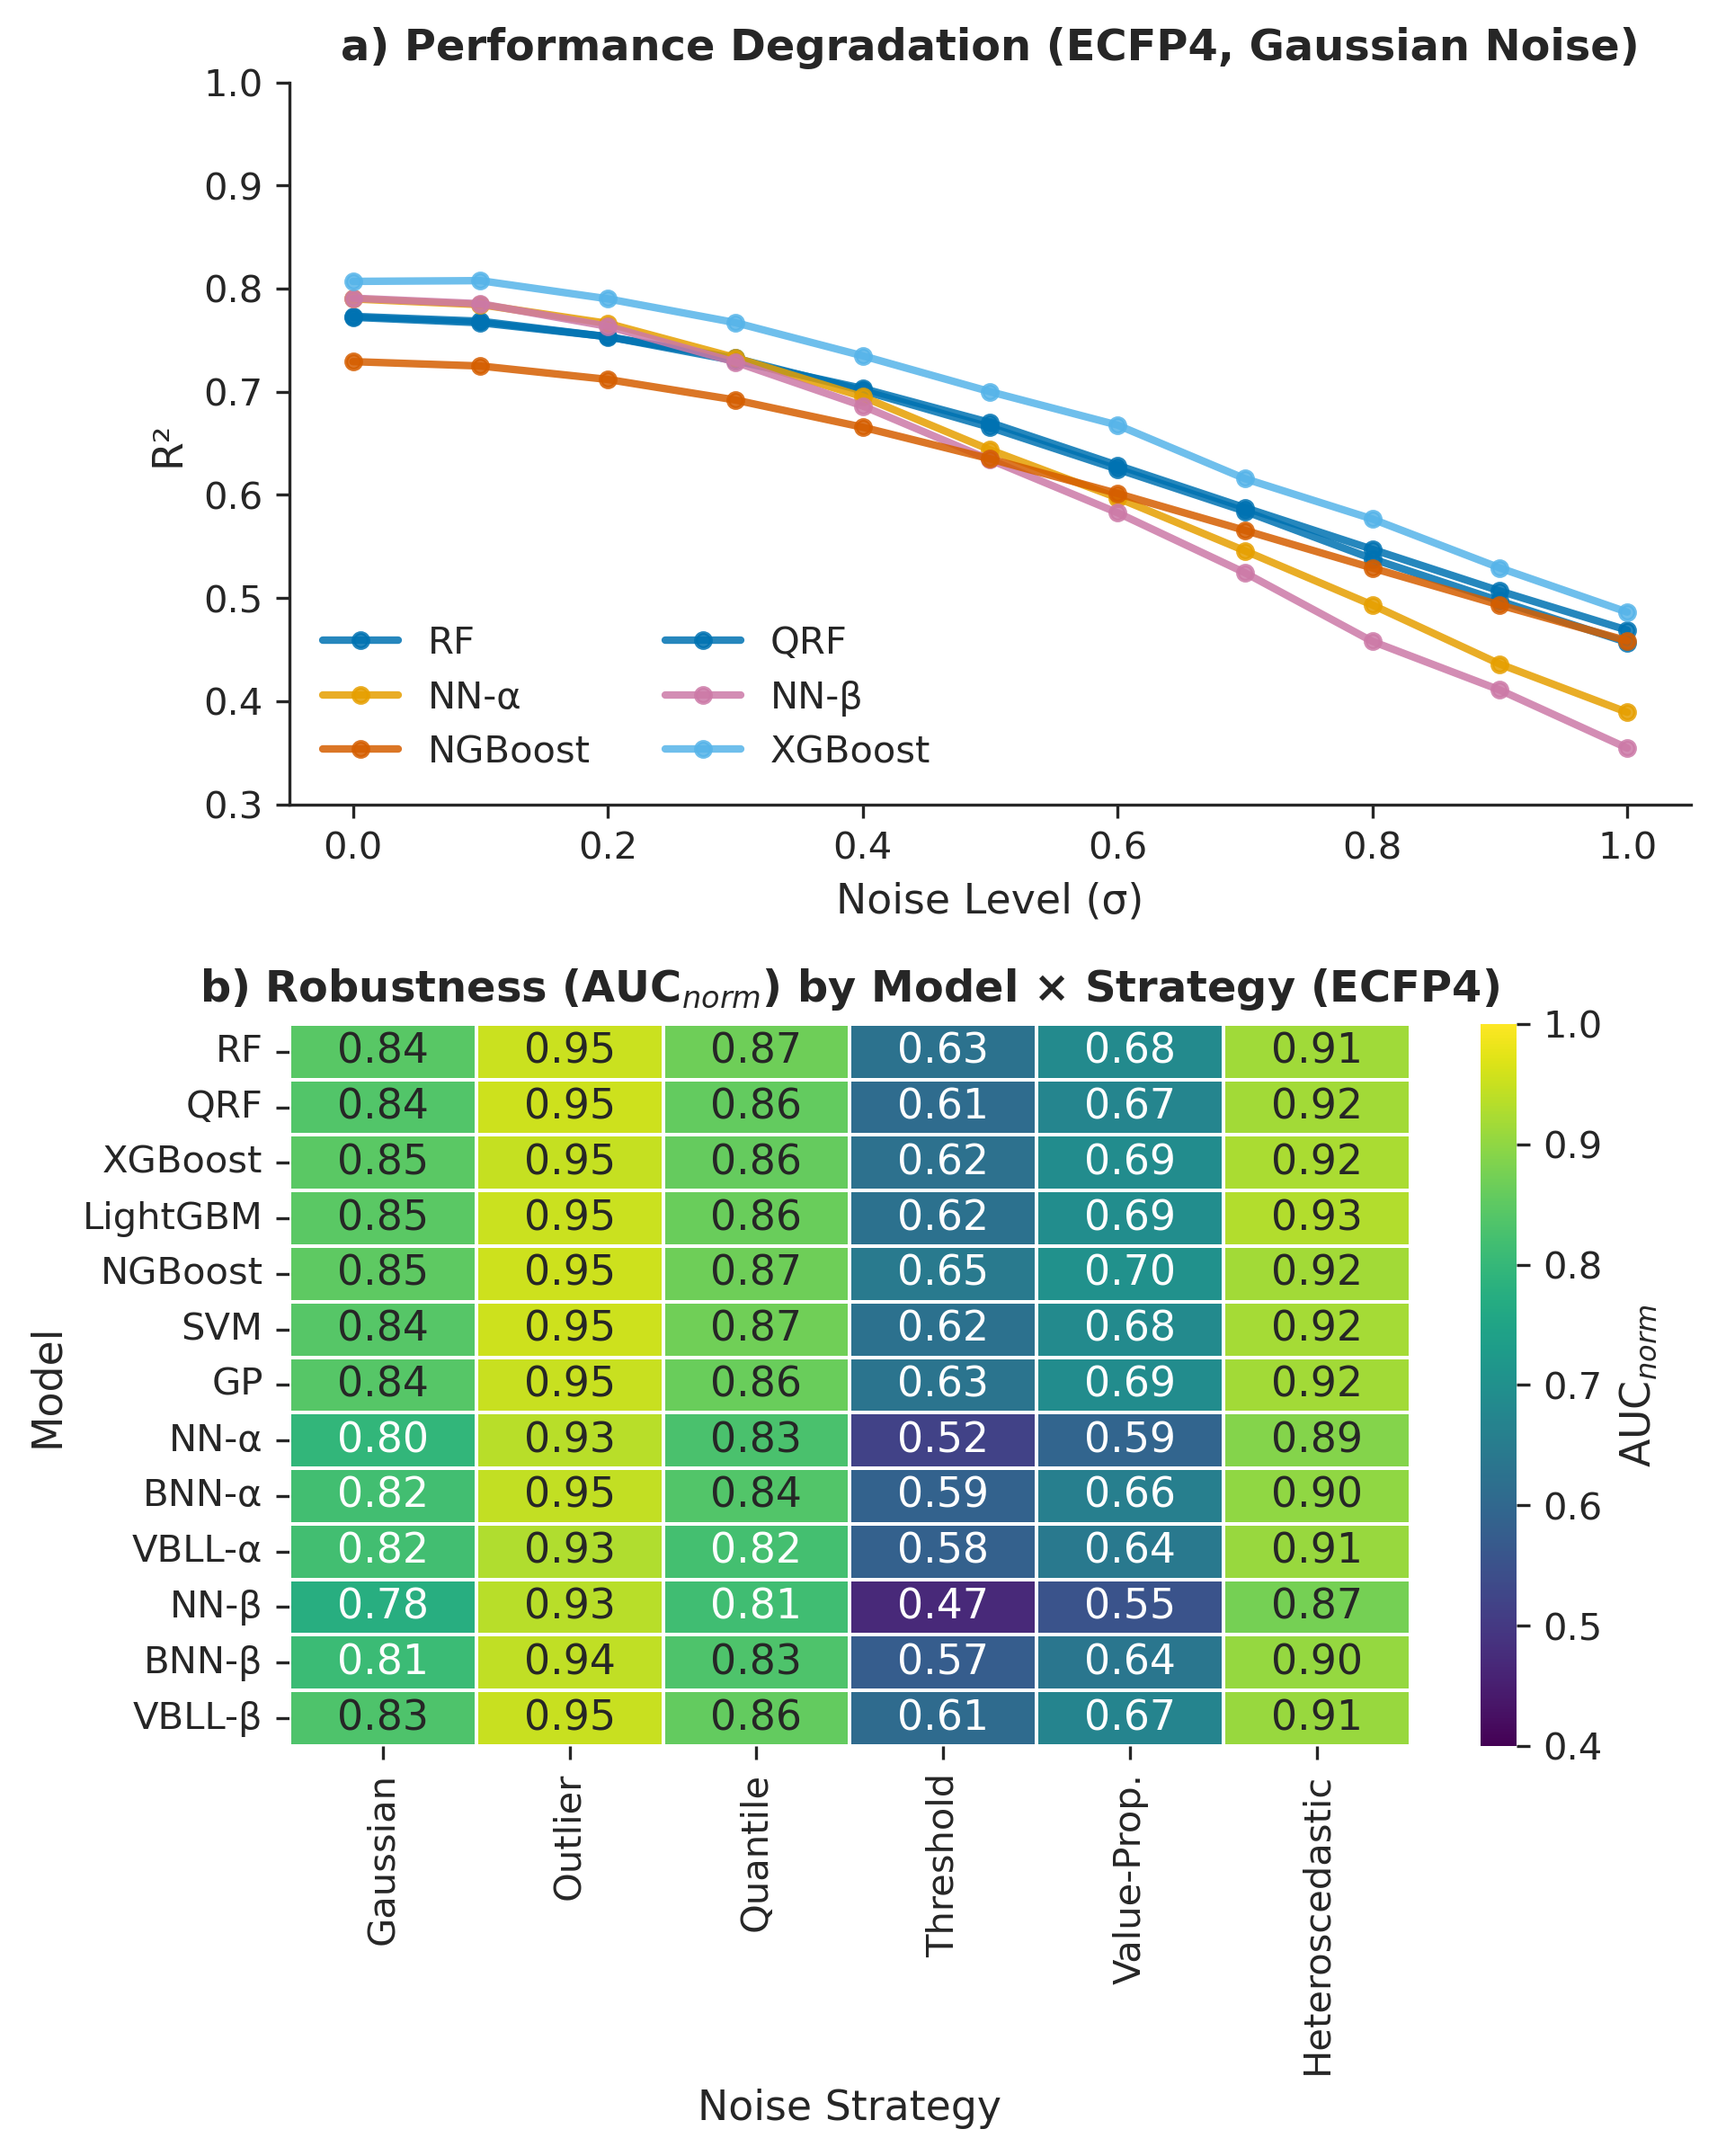
\includegraphics[width=\textwidth,height=0.78\textheight,keepaspectratio]{fig1_supp_ecfp4_overview.png}
\caption{\textbf{Global overview of noise robustness on the ECFP4 representation, evaluated on QM9 HOMO--LUMO gap.}
a) Performance degradation curves (R$^2$ versus noise level $\sigma$) under Gaussian noise. b) Noise degradation slope (NDS) heatmap across model architectures and noise strategies; lower (more negative) NDS indicates faster degradation under noise.}
\label{app:noise:ecfp4_overview}
\end{figure}


\section{Clean $R^2$ against robustness, PDV, Gaussian noise}\label{app:noise:sec:clean_r2_vs_robustness}
% Thesis appendix item: clean_r2_vs_robustness
% Seeded on 2026-09-27 from qsar_qm_models/supplementary/items/clean_r2_vs_robustness.tex by thesis_appendix/seed_from_paper.py.
% From here on this copy is edited independently of the paper. Rules: thesis_appendix/README.md.
% The lines below, down to the first blank line, are the PAPER copy's header, kept for
% provenance. They describe the paper file, not this one: in particular a GENERATED
% notice there does not apply here, and this copy may be edited by hand.
% Supplementary item: clean_r2_vs_robustness
% Split out of additional_files.tex on 2026-09-27, where it was Additional file 7 (Baseline R^2 vs NDS scatter (was Supp Figure S2)).
% Content unchanged apart from: the heading line removed (the build writes it), the old
% 'Table S*/Figure S*' caption prefix replaced by \SuppFile{}, and the label renamed to supp:clean_r2_vs_robustness.
% Rules: supplementary/README.md.

\begin{figure}[H]
\centering
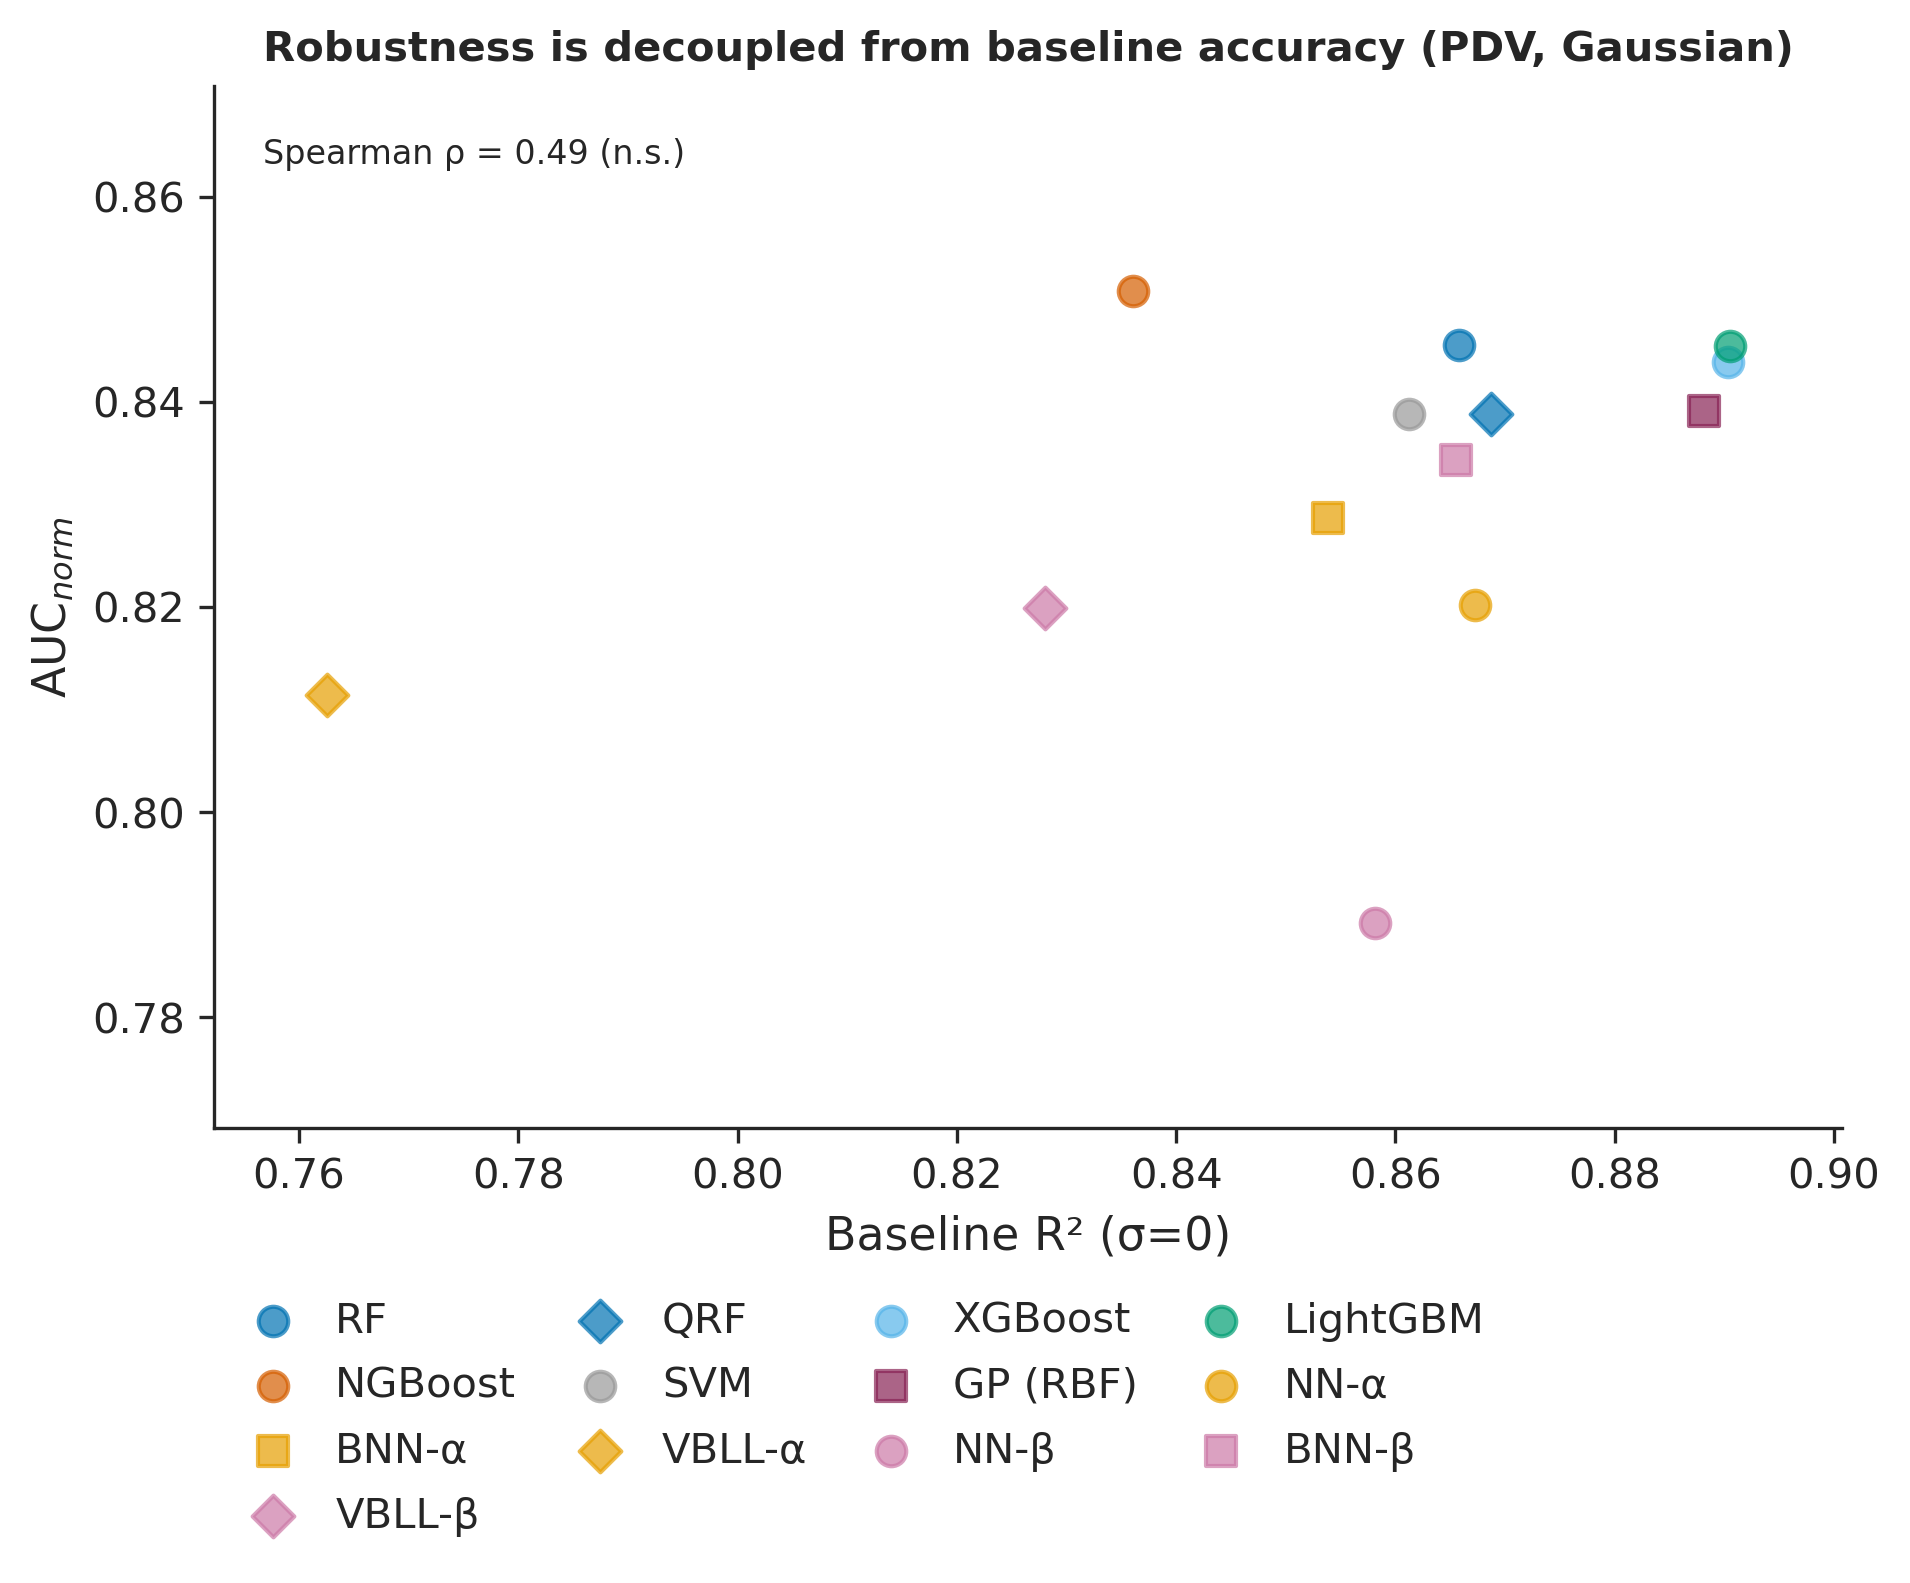
\includegraphics[width=\textwidth]{fig3_ranking_consistency.png}
\caption{\textbf{Baseline R$^2$ versus noise degradation slope (NDS) scatter for all models on the physicochemical descriptor vector (PDV) representation under Gaussian noise, on the QM9 HOMO--LUMO gap.}
Lower (more negative) NDS indicates faster performance loss under noise.}
\label{app:noise:clean_r2_vs_robustness}
\end{figure}


\section{Bayesian transformation effects by representation}\label{app:noise:sec:bayesian_transformation_tests}
% Thesis appendix item: bayesian_transformation_tests
% Seeded on 2026-09-27 from qsar_qm_models/supplementary/items/bayesian_transformation_tests.tex by thesis_appendix/seed_from_paper.py.
% From here on this copy is edited independently of the paper. Rules: thesis_appendix/README.md.
% The lines below, down to the first blank line, are the PAPER copy's header, kept for
% provenance. They describe the paper file, not this one: in particular a GENERATED
% notice there does not apply here, and this copy may be edited by hand.
% Supplementary item: bayesian_transformation_tests
% Split out of additional_files.tex on 2026-09-27, where it was Additional file 8 (NN Bayesian transformation effects (was Supp Table S6)).
% Content unchanged apart from: the heading line removed (the build writes it), the old
% 'Table S*/Figure S*' caption prefix replaced by \SuppFile{}, and the label renamed to supp:bayesian_transformation_tests.
% Rules: supplementary/README.md.

\begin{table}[H]
\centering
\caption{\textbf{Neural network Bayesian transformation effects on noise degradation slope (NDS) by representation, on the QM9 HOMO--LUMO gap.}
Positive $\Delta$ NDS indicates the Bayesian variant is more robust (less negative slope) than its deterministic counterpart.}
\label{app:noise:bayesian_transformation_tests}
\small
\begin{tabular}{llrrrr}
\toprule
\textbf{Model} & \textbf{Representation} & \textbf{Baseline R$^2$} & \textbf{NN-$\beta$ NDS} & \textbf{BNN-$\beta$ NDS} & \textbf{$\Delta$ NDS} \\
\midrule
NN-$\beta$ & ECFP4 & 0.791 & $-0.464$ & $-0.388$ & $+0.076$ \\
NN-$\beta$ & PDV & 0.858 & $-0.487$ & $-0.382$ & $+0.106$ \\
NN-$\beta$ & SMILES & 0.721 & $-0.558$ & $-0.365$ & $+0.193$ \\
\bottomrule
\end{tabular}
\end{table}


\section{Uncertainty metrics for probabilistic models on ECFP4}\label{app:noise:sec:uncertainty_metrics_ecfp4}
% Thesis appendix item: uncertainty_metrics_ecfp4
% Seeded on 2026-09-27 from qsar_qm_models/supplementary/items/uncertainty_metrics_ecfp4.tex by thesis_appendix/seed_from_paper.py.
% From here on this copy is edited independently of the paper. Rules: thesis_appendix/README.md.
% The lines below, down to the first blank line, are the PAPER copy's header, kept for
% provenance. They describe the paper file, not this one: in particular a GENERATED
% notice there does not apply here, and this copy may be edited by hand.
% Supplementary item: uncertainty_metrics_ecfp4
% Split out of additional_files.tex on 2026-09-27, where it was Additional file 9 (Uncertainty metrics ECFP4 (was Supp Table S8)).
% Content unchanged apart from: the heading line removed (the build writes it), the old
% 'Table S*/Figure S*' caption prefix replaced by \SuppFile{}, and the label renamed to supp:uncertainty_metrics_ecfp4.
% Rules: supplementary/README.md.

\begin{table}[H]
\centering
\caption{\textbf{Uncertainty quantification metrics for probabilistic models on the ECFP4 representation (Gaussian noise strategy) on the QM9 HOMO--LUMO gap.}
Unc-Error $\rho$: Spearman correlation between predicted uncertainty and absolute prediction error. Unc-Noise $\rho$: Spearman correlation between predicted uncertainty and injected noise level $\sigma$. ECE: expected calibration error (lower = better-calibrated). Coverage targets: 68\% ($1\sigma$), 95\% ($2\sigma$).}
\label{app:noise:uncertainty_metrics_ecfp4}
\small
\begin{tabular}{lrrrrr}
\toprule
\textbf{Model} & \textbf{Unc-Error $\rho$} & \textbf{Unc-Noise $\rho$} & \textbf{ECE} & \textbf{Cov.\ $1\sigma$} & \textbf{Cov.\ $2\sigma$} \\
\midrule
\textbf{QRF}     & \textbf{0.25} & 0.27 & 0.19 & 74.7\% & 94.6\% \\
\textbf{NGBoost} & 0.22 & \textbf{0.37} & \textbf{0.11} & 69.2\% & 94.2\% \\
GP               & 0.18 & 0.34 & 0.23 & 78.6\% & 96.0\% \\
BNN-$\beta$      & 0.20 & 0.37 & 0.29 & 78.6\% & 95.2\% \\
BNN-$\alpha$     & 0.15 & 0.32 & 0.24 & 76.6\% & 95.1\% \\
VBLL-$\beta$     & 0.19 & 0.34 & 0.19 & 73.9\% & 95.5\% \\
VBLL-$\alpha$    & 0.11 & 0.31 & 0.22 & 74.5\% & 95.1\% \\
\bottomrule
\end{tabular}
\end{table}


\section{Variance decomposition on the three assay datasets}\label{app:noise:sec:assay_variance_decomposition}
% Thesis appendix item: assay_variance_decomposition
% Seeded on 2026-09-27 from qsar_qm_models/supplementary/items/assay_variance_decomposition.tex by thesis_appendix/seed_from_paper.py.
% From here on this copy is edited independently of the paper. Rules: thesis_appendix/README.md.
% The lines below, down to the first blank line, are the PAPER copy's header, kept for
% provenance. They describe the paper file, not this one: in particular a GENERATED
% notice there does not apply here, and this copy may be edited by hand.
% Supplementary item: assay_variance_decomposition
% Split out of additional_files.tex on 2026-09-27, where it was Additional file 10 (Validation ANOVA (was Supp Figure S3)).
% Content unchanged apart from: the heading line removed (the build writes it), the old
% 'Table S*/Figure S*' caption prefix replaced by \SuppFile{}, and the label renamed to supp:assay_variance_decomposition.
% Rules: supplementary/README.md.

\begin{figure}[H]
\centering
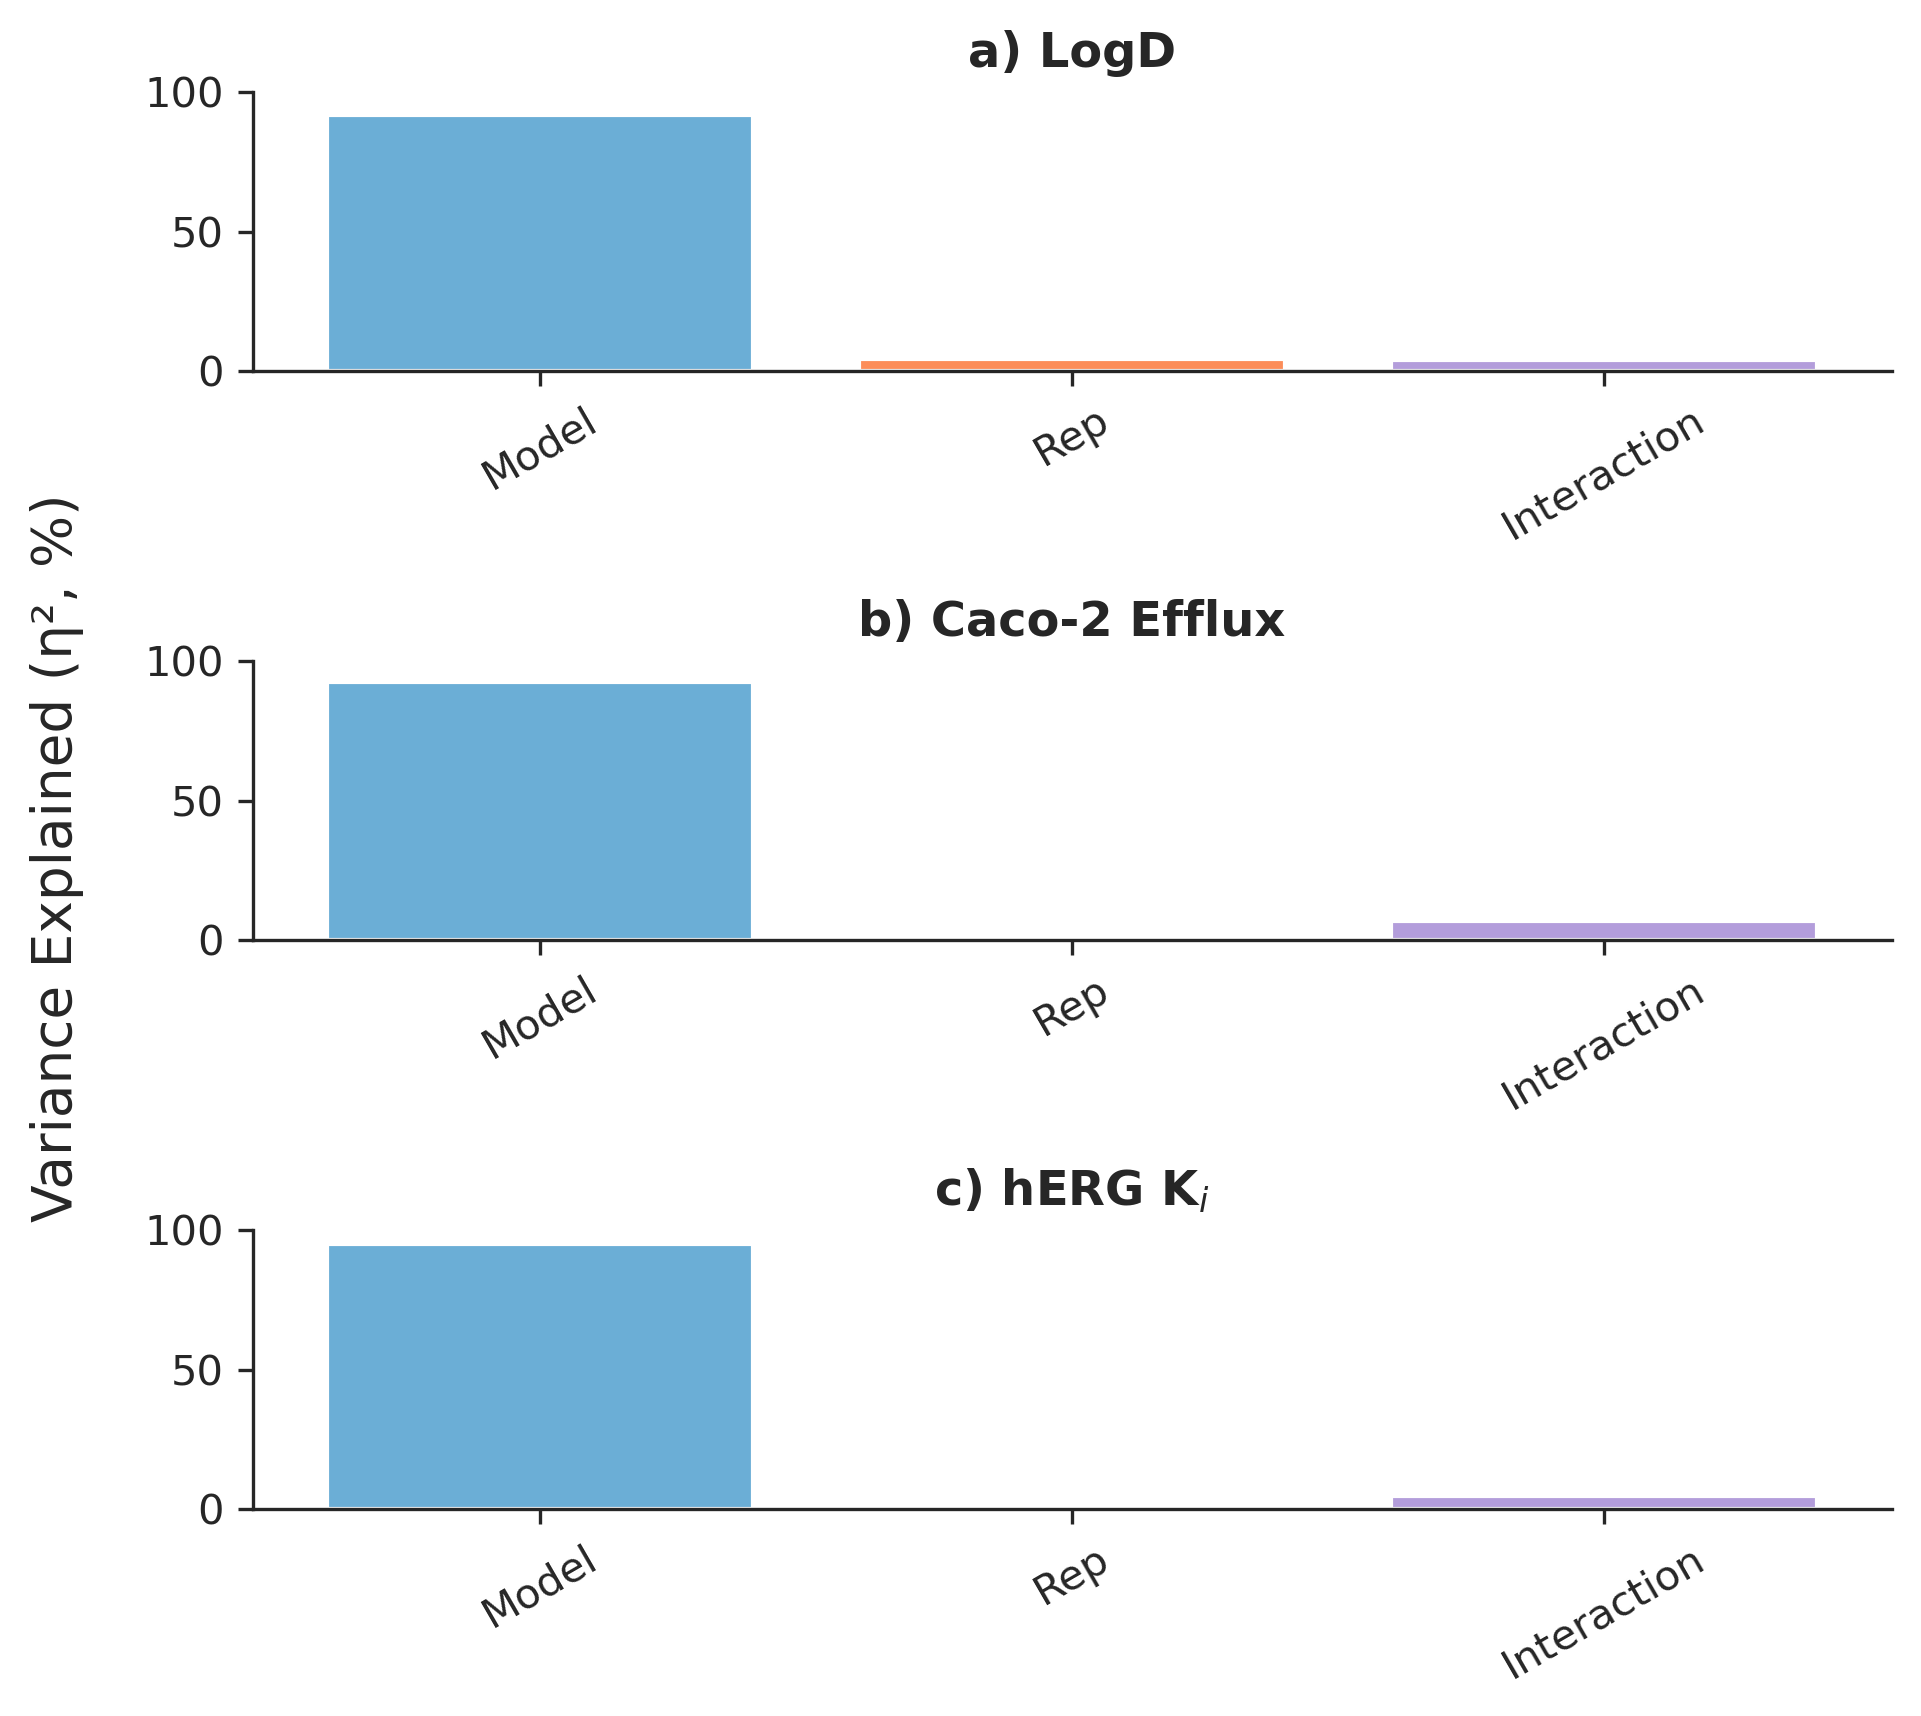
\includegraphics[width=\textwidth]{fig_validation_anova.png}
\caption{\textbf{ANOVA variance decomposition ($\eta^2$, \%) on external validation datasets: a) LogD, b) Caco-2 Efflux, and c) hERG K$_i$.}
Model, representation, and interaction contributions to noise degradation slope (NDS) variance for each dataset; lower (more negative) NDS indicates faster performance loss under noise.}
\label{app:noise:assay_variance_decomposition}
\end{figure}


\section{RF against QRF on the three assay datasets}\label{app:noise:sec:rf_vs_qrf_assay}
% Thesis appendix item: rf_vs_qrf_assay
% Seeded on 2026-09-27 from qsar_qm_models/supplementary/items/rf_vs_qrf_assay.tex by thesis_appendix/seed_from_paper.py.
% From here on this copy is edited independently of the paper. Rules: thesis_appendix/README.md.
% The lines below, down to the first blank line, are the PAPER copy's header, kept for
% provenance. They describe the paper file, not this one: in particular a GENERATED
% notice there does not apply here, and this copy may be edited by hand.
% Supplementary item: rf_vs_qrf_assay
% Split out of additional_files.tex on 2026-09-27, where it was Additional file 11 (RF vs QRF on validation datasets (was Supp Table S7)).
% Content unchanged apart from: the heading line removed (the build writes it), the old
% 'Table S*/Figure S*' caption prefix replaced by \SuppFile{}, and the label renamed to supp:rf_vs_qrf_assay.
% Rules: supplementary/README.md.

\begin{table}[H]
\centering
\caption{\textbf{Random forest (RF) vs quantile regression forest (QRF) noise degradation slope (NDS) on the three external validation datasets (LogD, Caco-2 Efflux, hERG K$_i$).}
Lower (more negative) NDS indicates faster degradation under noise.}
\label{app:noise:rf_vs_qrf_assay}
\small
\begin{tabular}{lrrr}
\toprule
\textbf{Dataset} & \textbf{RF NDS} & \textbf{QRF NDS} & \textbf{$\Delta$ NDS} \\
\midrule
ChEMBL-hERG-Ki     & $-0.231$ & $-0.359$ & $-0.128$ \\
OpenADMET-Caco2    & $-0.534$ & $-0.627$ & $-0.094$ \\
OpenADMET-LogD     & $-0.101$ & $-0.185$ & $-0.083$ \\
\bottomrule
\end{tabular}
\end{table}


\chapter{The search space and its defaults}\label{app:searchspace}
% ---- from THESIS_OUTLINE.md :: APPENDIX C (quoted; long bullets condensed) ----
%   C: the method's full search space and the design-experiment tables behind its defaults (Chapter 4).
%      The full vocabulary: downstream models (rf, xgboost, ridge, knn, lightgbm,
%      mlp, svm, gp, with optional catboost, dnn, cnn, bnn, ngboost); feature budgets (roughly 10
%      to 2,000, per-model capped); allocation methods (greedy, performance-weighted with its
%      weighting schemes, dominant-greedy, fixed, two-stage, stability-selection); importance
%      methods (treeshap, xgboost_gain, lightgbm_gain, permutation, kernelshap, deeplift,
%      integrated_gradients, gradientshap); internal evaluators (match, or rf/svm/lightgbm/mlp);
%      augmentation strategies; and the exact blueprint fields.
% ---- end outline extract ----
\todo[inline, color=orange!40]{Appendix C is unwritten.}
\chapter{Extended result tables}\label{app:results}
% ---- from THESIS_OUTLINE.md :: APPENDIX D (quoted; long bullets condensed) ----
%   D: extended result tables for the second-half chapters (Chapters 5 to 6), organised by the
%      featured experiments: the cross-domain summary; the information-theoretic decomposition;
%      the explainability and attribution tables; the forward-compatibility tables; the federated
%      comparator tables; the similarity-activity correlation tables; the BindingDB
%      ground-truth-noise table; and the remediation and noise-estimation tables.
% ---- end outline extract ----
\todo[inline, color=orange!40]{Appendix D is unwritten.}
\chapter{Data and code availability}\label{app:availability}
% ---- from THESIS_OUTLINE.md :: APPENDIX E (quoted; long bullets condensed) ----
%   E: data and code availability (all chapters). The full statement covers three distinct
%      software artifacts. (1) NoiseInject: the open-source benchmarking framework, MIT, at
%      github.com/adpunt/noise_inject, archived on Zenodo; released. (2) The standalone Rust and
%      Python chemical-processing and precompute pipeline. (3) The KIRBy research codebase: pure
%      Python. KIRBy contains no Rust; it operates on precomputed numpy feature matrices.
% ---- end outline extract ----

% [NI 629-640] her NoiseInject availability statement + the Springer-style itemised
% block the outline asks for. Two more such blocks are needed (precompute pipeline, KIRBy).
The NoiseInject benchmarking framework, implementing all six regression and six classification noise injection strategies together with the robustness metrics (noise degradation slope and retention) and uncertainty-calibration metrics (ECE, coverage at $1\sigma$/$2\sigma$, mean interval width, and uncertainty--error / uncertainty--noise correlation) described in this work, is available as an open-source Python package under an MIT license \citep{noiseinject}. It also contains optional reference wrappers (a Gaussian process, split-conformal prediction, and Monte Carlo dropout) that produce per-sample uncertainty for use with these metrics. NoiseInject is model-agnostic, operates on label arrays (NumPy arrays or pandas Series), and is designed to integrate into existing cheminformatics or other data pipelines. Worked examples covering molecular-descriptor, fingerprint, and GNN-embedding workflows are provided in the repository.

\begin{itemize}
    \item Project name: NoiseInject
    \item Project home page: \url{https://github.com/adpunt/noise_inject}
    \item Archived version: \url{https://doi.org/10.5281/zenodo.20532710}
    \item Operating system(s): Platform independent
    \item Programming language: Python
    \item Other requirements: See repository \texttt{requirements.txt} for the full dependency list
    \item License: MIT
    \item Any restrictions to use by non-academics: None
\end{itemize}

% [NI 654] authors' contributions, for the front-matter declaration.
A.P. implemented the NoiseInject framework, conducted all experiments, and drafted the manuscript. T.H., S.W., and G.M. supervised the project, contributed to the experimental design, and revised the manuscript. All authors read and approved the final manuscript.
\todo[inline, color=orange!40]{Appendix E: add itemised blocks for the Rust/Python precompute pipeline and for KIRBy, plus the Lhasa/Effiris redistribution caveat.}


%%============================== BIBLIOGRAPHY ===============================
\bibliographystyle{plainnat}
\bibliography{refs}

\end{document}
